\section{Motion Planning using Bicycle Model} \label{sec:motion_planning_using_bicylce}
Instead of using the double integrator model, we can employ the bicycle model to represent vehicle dynamics more accurately.
We have already introduced the bicycle model with a steering angle and an orientation in Section~\ref{subsec:bicycle_model}.
Now, we will combine this model with the concepts from the previous chapter.
Our objective is to represent the state variables in the road-aligned frame.
The state and control variables of the bicycle model, defined in the global coordinate system, are given in equations \eqref{eq:states_kst} and
\eqref{eq:controls_kst}.

\subsection{Transforming Global Cartesian Coordinates to Frenet Frame} \label{subsec:bicycle_conversion_of_cartesian_to_frenet}

In this section, we derive the state transition model in the Frenet frame.

We begin by considering the dynamics of the bicycle model in the global coordinate system, which are described by
\eqref{eq:kst_dpx}-\eqref{eq:dpsi_steering_angle}.

To express vehicle motion in the Frenet frame, we define the deviation from the reference path using the lateral displacement $n$ and the alignment
error $\xi = \psi - \theta$, where $\theta$ is the heading of the reference path.
The path curvature $C(s)$ relates to its arc length parameter $s$ as $\dot{\theta} = C(s) \dot{s}$.

Using the previously derived equations \eqref{eq:first_derivative_long} and \eqref{eq:first_derivative_lat}, we obtain the state transition equations in the Frenet frame:

\begin{align} \dot{s} &= \frac{v\cos\xi}{1 - nC(s)} \\ \dot{n} &= v\sin\xi \\ \dot{\xi} &= \dot{\psi} - C(s)\dot{s} \end{align}

By integrating these equations with the bicycle model, we derive a complete state transition model in the Frenet frame.
The state variables and control inputs for the bicycle model in the Frenet frame are defined in \eqref{def:kst_frenet_states} and
\eqref{def:kst_frenet_controls}.
\begin{align}
	x_{kst} & = \begin{bmatrix}
		            s & n & \xi & v & \delta
	            \end{bmatrix}^T
	\label{def:kst_frenet_states}        \\[10pt]
	u_{kst} & = \begin{bmatrix}
		            a & v_\delta
	            \end{bmatrix}^T
	\label{def:kst_frenet_controls}
\end{align}

The dynamics of the model are described by \eqref{eq:kst_frenet_dynamics}.

\begin{equation}
	f_{kst}(x_{kst}, u_{kst}) =
	\begin{bmatrix}
		\frac{v \cos\xi}{1 - nC(s)}                \\[8pt]
		v \sin\xi                                  \\[8pt]
		\frac{1}{l_{wb}}v \tan\delta - C(s)\dot{s} \\[8pt]
		a                                          \\[8pt]
		v_\delta
	\end{bmatrix}.
	\label{eq:kst_frenet_dynamics}
\end{equation}

In the following section, we will present an approach how the model dynamics can be approximated to apply to the DCP rules.

\subsection{Model Dynamics Approximation} \label{subsec:approximation_of_model_dynamics}

For this model, we will stick to the body-fixed control inputs, which keeps the coupling constraints convex.
Instead, we aim to linearize the model dynamics using two new techniques.
These techniques allow us to maintain the constraints without shifting, as was necessary in the previous chapter.
This ensures a more accurate and computationally efficient representation of the vehicle's motion.

To simplify the model, we make the following assumption: $nC(s)$ is close to zero.
This is valid since $n$ represents the vehicle's lateral position relative to the reference path, and $C(s)$ is the curvature of the reference path,
which is typically small enough for this assumption to hold.
We will analyze the terms that introduce nonlinearity into the model.

\subsubsection{Nonlinear Terms}

The state transition model contains four nonlinear terms.
We will linearize these terms using appropriate approximations.
\[
	\frac{v \cos\xi}{1 - nC(s)} ,
	v \sin\xi                   ,
	v \tan\delta                ,
	C(s)\dot{s}
\]

Given our assumption that $nC(s) \approx 0$, we can simplify the first term as follows:

\[ \frac{v \cos\xi}{1 - nC(s)} \approx v
	\cos\xi \]

\subsubsection{First Order Taylor Polynomial} To linearize the trigonometric terms, we use the first-order
approximation around a reference point.
The first-order Taylor expansion of a function $f(x)$ around a point $x_0$ is given by:

\[ f(x) \approx f(x_0) + \frac{df}{dx}
	(x_0) (x - x_0) \]

Using the first-order Taylor polynomial to approximate the trigonometric functions $\sin$, $\cos$, and $\tan$
around the reference points $\xi_0$ and $\delta_0$, we obtain the following linearization:

\[ \cos(\xi) \approx \cos(\xi_0) -
	\sin(\xi_0) (\xi - \xi_0) \] \[ \sin(\xi) \approx \sin(\xi_0) + \cos(\xi_0) (\xi - \xi_0) \] \[ \tan(\delta) \approx \tan(\delta_0) +
	\frac{1}{\cos^2(\delta_0)} (\delta - \delta_0) \]

These approximations are known as small angle approximations, which are valid
when the angles $\xi$ and $\delta$ are close to their reference values.
In vehicle dynamics, it is often reasonable to assume that the heading alignment error $\xi$ and the steering angle $\delta$ do not change rapidly,
especially when the vehicle is closely following a reference path.
This allows us to simplify the trigonometric functions using their first-order Taylor expansions.

By substituting these approximations into the state transition model, we obtain the following terms:
\begin{align*}
	 & v (\cos(\xi_0) - \sin(\xi_0) (\xi - \xi_0))                         \\
	 & v (\sin(\xi_0) + \cos(\xi_0) (\xi - \xi_0))                         \\
	 & v (\tan(\delta_0) + \frac{1}{\cos^2(\delta_0)} (\delta - \delta_0))
\end{align*}
Since our reference values $\xi_0$ and $\delta_0$ are treated as constants during planning, the only remaining nonlinear terms are: $$v \xi, v
	\delta, C(s)\dot{s}$$

These are known as bilinear terms, which occur when the product of two variables appears in the equations,
rendering the system nonlinear.
Since $C(s)$ is a function of $s$, we will introduce an additional assumption.
As discussed in \nameref{subsubsec:limitations_on_qe}, segmenting the road model helps reduce conservatism in coupling constraints, a technique we
previously applied to the double integrator model.
In this context, another advantage is that we can model the curvature as a piecewise linear function, which will be beneficial in subsequent steps.

\subsubsection{Assumption: Piecewise Linear Curvature}

We assume that the curvature can be approximated as a piecewise linear function.

\[
	C(s) = \begin{cases}
		a_1s+b_1 & \text{if } s \in [s_0, s_1]     \\
		a_2s+b_2 & \text{if } s \in [s_1, s_2]     \\
		\vdots                                     \\
		a_ns+b_n & \text{if } s \in [s_{n-1}, s_n]
	\end{cases}
\]

This transformation reduces the nonlinear term $C(s)\dot{s}$ to a bilinear term $s\dot{s}$, which still requires linearization.

In the next section, we will introduce a relaxation method to achieve this.

\subsection{Convex Relaxation of Bilinear Terms} \label{subsec:convex_relaxation_for_bilinear_terms}

To handle bilinear terms of the form $v_1v_2$, we introduce a new variable $w$ and apply the McCormick relaxation.
The McCormick relaxation is a technique that linearizes bilinear terms by introducing auxiliary variables and
constraints~\cite{mccormick_computability_1976}.
This technique allows us to represent the bilinear terms as a set of linear constraints, which can be solved efficiently using convex optimization
methods.
This relaxation only works if the variables $v_1$ and $v_2$ are bounded:

\[ \underline{v_1} \leq v_1 \leq \overline{v_1}, \qquad
	\underline{v_2} \leq v_2 \leq \overline{v_2} \] with constants $\underline{v_1}, \overline{v_1}, \underline{v_2}, \overline{v_2} \in \mathbb{R}$.

We introduce an auxiliary variable $w$ to approximate the bilinear term $v_1v_2$.
Linear constraints are applied to bound $w$ and ensure it accurately represents the bilinear term $v_1v_2$.
These constraints are derived from the bounds of the variables $v_1$, $v_2$, and the bilinear term $v_1v_2$, as shown below:

\[
	\begin{aligned}
		w & \geq \underline{v_1} v_2 + v_1 \underline{v_2} - \underline{v_1} \underline{v_2}, \\
		w & \geq \overline{v_1} v_2 + v_1 \overline{v_2} - \overline{v_1} \overline{v_2},     \\
		w & \leq \overline{v_1} v_2 + v_1 \underline{v_2} - \overline{v_1} \underline{v_2},   \\
		w & \leq \underline{v_1} v_2 + v_1 \overline{v_2} - \underline{v_1} \overline{v_2}.
	\end{aligned}
\]
The idea behind these constraints is to create a convex lower bound and a concave upper bound for the bilinear term $v_1v_2$.
For example, the first bound is constructed as follows: \[ a = (v_1 - \underline{v_1}) \geq 0, b = (v_2 - \underline{v_2}) \geq 0 \] Since $a$ and
$b$ are both non-negative, we can multiply them to obtain our first lower bound: \[ ab = v_1v_2 - \underline{v_1}v_2 - v_1\underline{v_2} +
	\underline{v_1}\underline{v_2} \geq 0 \iff v_1v_2 \geq \underline{v_1}v_2 + v_1\underline{v_2} - \underline{v_1}\underline{v_2} \]

To derive all possible lower and upper bounds, we can apply this pattern to $a \in \{v_1 - \underline{v_1}, \overline{v_1} -
	v_1\}$ and $b \in \{v_2 - \underline{v_2}, \overline{v_2} - v_2\}$.
For any of the four possible combinations of $a$ and $b$, we get $ab \geq 0$ and can therefore establish either an upper or lower bound for $v_1v_2$.

\begin{figure}[h]
	\centering
	\begin{subfigure}[b]{0.45\textwidth}
		\centering
		\resizebox{\textwidth}{!}{%% Creator: Matplotlib, PGF backend
%%
%% To include the figure in your LaTeX document, write
%%   \input{<filename>.pgf}
%%
%% Make sure the required packages are loaded in your preamble
%%   \usepackage{pgf}
%%
%% Also ensure that all the required font packages are loaded; for instance,
%% the lmodern package is sometimes necessary when using math font.
%%   \usepackage{lmodern}
%%
%% Figures using additional raster images can only be included by \input if
%% they are in the same directory as the main LaTeX file. For loading figures
%% from other directories you can use the `import` package
%%   \usepackage{import}
%%
%% and then include the figures with
%%   \import{<path to file>}{<filename>.pgf}
%%
%% Matplotlib used the following preamble
%%   \def\mathdefault#1{#1}
%%   \everymath=\expandafter{\the\everymath\displaystyle}
%%   
%%   \ifdefined\pdftexversion\else  % non-pdftex case.
%%     \usepackage{fontspec}
%%   \fi
%%   \makeatletter\@ifpackageloaded{underscore}{}{\usepackage[strings]{underscore}}\makeatother
%%
\begingroup%
\makeatletter%
\begin{pgfpicture}%
\pgfpathrectangle{\pgfpointorigin}{\pgfqpoint{4.377484in}{3.839102in}}%
\pgfusepath{use as bounding box, clip}%
\begin{pgfscope}%
\pgfsetbuttcap%
\pgfsetmiterjoin%
\definecolor{currentfill}{rgb}{1.000000,1.000000,1.000000}%
\pgfsetfillcolor{currentfill}%
\pgfsetlinewidth{0.000000pt}%
\definecolor{currentstroke}{rgb}{1.000000,1.000000,1.000000}%
\pgfsetstrokecolor{currentstroke}%
\pgfsetdash{}{0pt}%
\pgfpathmoveto{\pgfqpoint{0.000000in}{0.000000in}}%
\pgfpathlineto{\pgfqpoint{4.377484in}{0.000000in}}%
\pgfpathlineto{\pgfqpoint{4.377484in}{3.839102in}}%
\pgfpathlineto{\pgfqpoint{0.000000in}{3.839102in}}%
\pgfpathlineto{\pgfqpoint{0.000000in}{0.000000in}}%
\pgfpathclose%
\pgfusepath{fill}%
\end{pgfscope}%
\begin{pgfscope}%
\pgfsetbuttcap%
\pgfsetmiterjoin%
\definecolor{currentfill}{rgb}{1.000000,1.000000,1.000000}%
\pgfsetfillcolor{currentfill}%
\pgfsetlinewidth{0.000000pt}%
\definecolor{currentstroke}{rgb}{0.000000,0.000000,0.000000}%
\pgfsetstrokecolor{currentstroke}%
\pgfsetstrokeopacity{0.000000}%
\pgfsetdash{}{0pt}%
\pgfpathmoveto{\pgfqpoint{0.516434in}{0.499074in}}%
\pgfpathlineto{\pgfqpoint{3.713060in}{0.499074in}}%
\pgfpathlineto{\pgfqpoint{3.713060in}{3.695699in}}%
\pgfpathlineto{\pgfqpoint{0.516434in}{3.695699in}}%
\pgfpathlineto{\pgfqpoint{0.516434in}{0.499074in}}%
\pgfpathclose%
\pgfusepath{fill}%
\end{pgfscope}%
\begin{pgfscope}%
\pgfpathrectangle{\pgfqpoint{0.516434in}{0.499074in}}{\pgfqpoint{3.196625in}{3.196625in}}%
\pgfusepath{clip}%
\pgfsys@transformshift{0.516434in}{0.499074in}%
\pgftext[left,bottom]{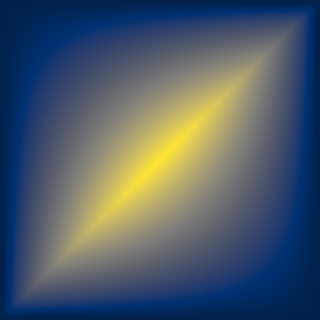
\includegraphics[interpolate=true,width=3.200000in,height=3.200000in]{figures/mccormick/mccormick-bounds-0-upper-img0.png}}%
\end{pgfscope}%
\begin{pgfscope}%
\pgfsetbuttcap%
\pgfsetroundjoin%
\definecolor{currentfill}{rgb}{0.000000,0.000000,0.000000}%
\pgfsetfillcolor{currentfill}%
\pgfsetlinewidth{0.803000pt}%
\definecolor{currentstroke}{rgb}{0.000000,0.000000,0.000000}%
\pgfsetstrokecolor{currentstroke}%
\pgfsetdash{}{0pt}%
\pgfsys@defobject{currentmarker}{\pgfqpoint{0.000000in}{-0.048611in}}{\pgfqpoint{0.000000in}{0.000000in}}{%
\pgfpathmoveto{\pgfqpoint{0.000000in}{0.000000in}}%
\pgfpathlineto{\pgfqpoint{0.000000in}{-0.048611in}}%
\pgfusepath{stroke,fill}%
}%
\begin{pgfscope}%
\pgfsys@transformshift{0.516434in}{0.499074in}%
\pgfsys@useobject{currentmarker}{}%
\end{pgfscope}%
\end{pgfscope}%
\begin{pgfscope}%
\definecolor{textcolor}{rgb}{0.000000,0.000000,0.000000}%
\pgfsetstrokecolor{textcolor}%
\pgfsetfillcolor{textcolor}%
\pgftext[x=0.516434in,y=0.401852in,,top]{\color{textcolor}{\rmfamily\fontsize{9.000000}{10.800000}\selectfont\catcode`\^=\active\def^{\ifmmode\sp\else\^{}\fi}\catcode`\%=\active\def%{\%}$\mathdefault{\ensuremath{-}2.0}$}}%
\end{pgfscope}%
\begin{pgfscope}%
\pgfsetbuttcap%
\pgfsetroundjoin%
\definecolor{currentfill}{rgb}{0.000000,0.000000,0.000000}%
\pgfsetfillcolor{currentfill}%
\pgfsetlinewidth{0.803000pt}%
\definecolor{currentstroke}{rgb}{0.000000,0.000000,0.000000}%
\pgfsetstrokecolor{currentstroke}%
\pgfsetdash{}{0pt}%
\pgfsys@defobject{currentmarker}{\pgfqpoint{0.000000in}{-0.048611in}}{\pgfqpoint{0.000000in}{0.000000in}}{%
\pgfpathmoveto{\pgfqpoint{0.000000in}{0.000000in}}%
\pgfpathlineto{\pgfqpoint{0.000000in}{-0.048611in}}%
\pgfusepath{stroke,fill}%
}%
\begin{pgfscope}%
\pgfsys@transformshift{0.916012in}{0.499074in}%
\pgfsys@useobject{currentmarker}{}%
\end{pgfscope}%
\end{pgfscope}%
\begin{pgfscope}%
\definecolor{textcolor}{rgb}{0.000000,0.000000,0.000000}%
\pgfsetstrokecolor{textcolor}%
\pgfsetfillcolor{textcolor}%
\pgftext[x=0.916012in,y=0.401852in,,top]{\color{textcolor}{\rmfamily\fontsize{9.000000}{10.800000}\selectfont\catcode`\^=\active\def^{\ifmmode\sp\else\^{}\fi}\catcode`\%=\active\def%{\%}$\mathdefault{\ensuremath{-}1.5}$}}%
\end{pgfscope}%
\begin{pgfscope}%
\pgfsetbuttcap%
\pgfsetroundjoin%
\definecolor{currentfill}{rgb}{0.000000,0.000000,0.000000}%
\pgfsetfillcolor{currentfill}%
\pgfsetlinewidth{0.803000pt}%
\definecolor{currentstroke}{rgb}{0.000000,0.000000,0.000000}%
\pgfsetstrokecolor{currentstroke}%
\pgfsetdash{}{0pt}%
\pgfsys@defobject{currentmarker}{\pgfqpoint{0.000000in}{-0.048611in}}{\pgfqpoint{0.000000in}{0.000000in}}{%
\pgfpathmoveto{\pgfqpoint{0.000000in}{0.000000in}}%
\pgfpathlineto{\pgfqpoint{0.000000in}{-0.048611in}}%
\pgfusepath{stroke,fill}%
}%
\begin{pgfscope}%
\pgfsys@transformshift{1.315591in}{0.499074in}%
\pgfsys@useobject{currentmarker}{}%
\end{pgfscope}%
\end{pgfscope}%
\begin{pgfscope}%
\definecolor{textcolor}{rgb}{0.000000,0.000000,0.000000}%
\pgfsetstrokecolor{textcolor}%
\pgfsetfillcolor{textcolor}%
\pgftext[x=1.315591in,y=0.401852in,,top]{\color{textcolor}{\rmfamily\fontsize{9.000000}{10.800000}\selectfont\catcode`\^=\active\def^{\ifmmode\sp\else\^{}\fi}\catcode`\%=\active\def%{\%}$\mathdefault{\ensuremath{-}1.0}$}}%
\end{pgfscope}%
\begin{pgfscope}%
\pgfsetbuttcap%
\pgfsetroundjoin%
\definecolor{currentfill}{rgb}{0.000000,0.000000,0.000000}%
\pgfsetfillcolor{currentfill}%
\pgfsetlinewidth{0.803000pt}%
\definecolor{currentstroke}{rgb}{0.000000,0.000000,0.000000}%
\pgfsetstrokecolor{currentstroke}%
\pgfsetdash{}{0pt}%
\pgfsys@defobject{currentmarker}{\pgfqpoint{0.000000in}{-0.048611in}}{\pgfqpoint{0.000000in}{0.000000in}}{%
\pgfpathmoveto{\pgfqpoint{0.000000in}{0.000000in}}%
\pgfpathlineto{\pgfqpoint{0.000000in}{-0.048611in}}%
\pgfusepath{stroke,fill}%
}%
\begin{pgfscope}%
\pgfsys@transformshift{1.715169in}{0.499074in}%
\pgfsys@useobject{currentmarker}{}%
\end{pgfscope}%
\end{pgfscope}%
\begin{pgfscope}%
\definecolor{textcolor}{rgb}{0.000000,0.000000,0.000000}%
\pgfsetstrokecolor{textcolor}%
\pgfsetfillcolor{textcolor}%
\pgftext[x=1.715169in,y=0.401852in,,top]{\color{textcolor}{\rmfamily\fontsize{9.000000}{10.800000}\selectfont\catcode`\^=\active\def^{\ifmmode\sp\else\^{}\fi}\catcode`\%=\active\def%{\%}$\mathdefault{\ensuremath{-}0.5}$}}%
\end{pgfscope}%
\begin{pgfscope}%
\pgfsetbuttcap%
\pgfsetroundjoin%
\definecolor{currentfill}{rgb}{0.000000,0.000000,0.000000}%
\pgfsetfillcolor{currentfill}%
\pgfsetlinewidth{0.803000pt}%
\definecolor{currentstroke}{rgb}{0.000000,0.000000,0.000000}%
\pgfsetstrokecolor{currentstroke}%
\pgfsetdash{}{0pt}%
\pgfsys@defobject{currentmarker}{\pgfqpoint{0.000000in}{-0.048611in}}{\pgfqpoint{0.000000in}{0.000000in}}{%
\pgfpathmoveto{\pgfqpoint{0.000000in}{0.000000in}}%
\pgfpathlineto{\pgfqpoint{0.000000in}{-0.048611in}}%
\pgfusepath{stroke,fill}%
}%
\begin{pgfscope}%
\pgfsys@transformshift{2.114747in}{0.499074in}%
\pgfsys@useobject{currentmarker}{}%
\end{pgfscope}%
\end{pgfscope}%
\begin{pgfscope}%
\definecolor{textcolor}{rgb}{0.000000,0.000000,0.000000}%
\pgfsetstrokecolor{textcolor}%
\pgfsetfillcolor{textcolor}%
\pgftext[x=2.114747in,y=0.401852in,,top]{\color{textcolor}{\rmfamily\fontsize{9.000000}{10.800000}\selectfont\catcode`\^=\active\def^{\ifmmode\sp\else\^{}\fi}\catcode`\%=\active\def%{\%}$\mathdefault{0.0}$}}%
\end{pgfscope}%
\begin{pgfscope}%
\pgfsetbuttcap%
\pgfsetroundjoin%
\definecolor{currentfill}{rgb}{0.000000,0.000000,0.000000}%
\pgfsetfillcolor{currentfill}%
\pgfsetlinewidth{0.803000pt}%
\definecolor{currentstroke}{rgb}{0.000000,0.000000,0.000000}%
\pgfsetstrokecolor{currentstroke}%
\pgfsetdash{}{0pt}%
\pgfsys@defobject{currentmarker}{\pgfqpoint{0.000000in}{-0.048611in}}{\pgfqpoint{0.000000in}{0.000000in}}{%
\pgfpathmoveto{\pgfqpoint{0.000000in}{0.000000in}}%
\pgfpathlineto{\pgfqpoint{0.000000in}{-0.048611in}}%
\pgfusepath{stroke,fill}%
}%
\begin{pgfscope}%
\pgfsys@transformshift{2.514325in}{0.499074in}%
\pgfsys@useobject{currentmarker}{}%
\end{pgfscope}%
\end{pgfscope}%
\begin{pgfscope}%
\definecolor{textcolor}{rgb}{0.000000,0.000000,0.000000}%
\pgfsetstrokecolor{textcolor}%
\pgfsetfillcolor{textcolor}%
\pgftext[x=2.514325in,y=0.401852in,,top]{\color{textcolor}{\rmfamily\fontsize{9.000000}{10.800000}\selectfont\catcode`\^=\active\def^{\ifmmode\sp\else\^{}\fi}\catcode`\%=\active\def%{\%}$\mathdefault{0.5}$}}%
\end{pgfscope}%
\begin{pgfscope}%
\pgfsetbuttcap%
\pgfsetroundjoin%
\definecolor{currentfill}{rgb}{0.000000,0.000000,0.000000}%
\pgfsetfillcolor{currentfill}%
\pgfsetlinewidth{0.803000pt}%
\definecolor{currentstroke}{rgb}{0.000000,0.000000,0.000000}%
\pgfsetstrokecolor{currentstroke}%
\pgfsetdash{}{0pt}%
\pgfsys@defobject{currentmarker}{\pgfqpoint{0.000000in}{-0.048611in}}{\pgfqpoint{0.000000in}{0.000000in}}{%
\pgfpathmoveto{\pgfqpoint{0.000000in}{0.000000in}}%
\pgfpathlineto{\pgfqpoint{0.000000in}{-0.048611in}}%
\pgfusepath{stroke,fill}%
}%
\begin{pgfscope}%
\pgfsys@transformshift{2.913903in}{0.499074in}%
\pgfsys@useobject{currentmarker}{}%
\end{pgfscope}%
\end{pgfscope}%
\begin{pgfscope}%
\definecolor{textcolor}{rgb}{0.000000,0.000000,0.000000}%
\pgfsetstrokecolor{textcolor}%
\pgfsetfillcolor{textcolor}%
\pgftext[x=2.913903in,y=0.401852in,,top]{\color{textcolor}{\rmfamily\fontsize{9.000000}{10.800000}\selectfont\catcode`\^=\active\def^{\ifmmode\sp\else\^{}\fi}\catcode`\%=\active\def%{\%}$\mathdefault{1.0}$}}%
\end{pgfscope}%
\begin{pgfscope}%
\pgfsetbuttcap%
\pgfsetroundjoin%
\definecolor{currentfill}{rgb}{0.000000,0.000000,0.000000}%
\pgfsetfillcolor{currentfill}%
\pgfsetlinewidth{0.803000pt}%
\definecolor{currentstroke}{rgb}{0.000000,0.000000,0.000000}%
\pgfsetstrokecolor{currentstroke}%
\pgfsetdash{}{0pt}%
\pgfsys@defobject{currentmarker}{\pgfqpoint{0.000000in}{-0.048611in}}{\pgfqpoint{0.000000in}{0.000000in}}{%
\pgfpathmoveto{\pgfqpoint{0.000000in}{0.000000in}}%
\pgfpathlineto{\pgfqpoint{0.000000in}{-0.048611in}}%
\pgfusepath{stroke,fill}%
}%
\begin{pgfscope}%
\pgfsys@transformshift{3.313482in}{0.499074in}%
\pgfsys@useobject{currentmarker}{}%
\end{pgfscope}%
\end{pgfscope}%
\begin{pgfscope}%
\definecolor{textcolor}{rgb}{0.000000,0.000000,0.000000}%
\pgfsetstrokecolor{textcolor}%
\pgfsetfillcolor{textcolor}%
\pgftext[x=3.313482in,y=0.401852in,,top]{\color{textcolor}{\rmfamily\fontsize{9.000000}{10.800000}\selectfont\catcode`\^=\active\def^{\ifmmode\sp\else\^{}\fi}\catcode`\%=\active\def%{\%}$\mathdefault{1.5}$}}%
\end{pgfscope}%
\begin{pgfscope}%
\pgfsetbuttcap%
\pgfsetroundjoin%
\definecolor{currentfill}{rgb}{0.000000,0.000000,0.000000}%
\pgfsetfillcolor{currentfill}%
\pgfsetlinewidth{0.803000pt}%
\definecolor{currentstroke}{rgb}{0.000000,0.000000,0.000000}%
\pgfsetstrokecolor{currentstroke}%
\pgfsetdash{}{0pt}%
\pgfsys@defobject{currentmarker}{\pgfqpoint{0.000000in}{-0.048611in}}{\pgfqpoint{0.000000in}{0.000000in}}{%
\pgfpathmoveto{\pgfqpoint{0.000000in}{0.000000in}}%
\pgfpathlineto{\pgfqpoint{0.000000in}{-0.048611in}}%
\pgfusepath{stroke,fill}%
}%
\begin{pgfscope}%
\pgfsys@transformshift{3.713060in}{0.499074in}%
\pgfsys@useobject{currentmarker}{}%
\end{pgfscope}%
\end{pgfscope}%
\begin{pgfscope}%
\definecolor{textcolor}{rgb}{0.000000,0.000000,0.000000}%
\pgfsetstrokecolor{textcolor}%
\pgfsetfillcolor{textcolor}%
\pgftext[x=3.713060in,y=0.401852in,,top]{\color{textcolor}{\rmfamily\fontsize{9.000000}{10.800000}\selectfont\catcode`\^=\active\def^{\ifmmode\sp\else\^{}\fi}\catcode`\%=\active\def%{\%}$\mathdefault{2.0}$}}%
\end{pgfscope}%
\begin{pgfscope}%
\definecolor{textcolor}{rgb}{0.000000,0.000000,0.000000}%
\pgfsetstrokecolor{textcolor}%
\pgfsetfillcolor{textcolor}%
\pgftext[x=2.114747in,y=0.235185in,,top]{\color{textcolor}{\rmfamily\fontsize{11.000000}{13.200000}\selectfont\catcode`\^=\active\def^{\ifmmode\sp\else\^{}\fi}\catcode`\%=\active\def%{\%}$v_1$}}%
\end{pgfscope}%
\begin{pgfscope}%
\pgfsetbuttcap%
\pgfsetroundjoin%
\definecolor{currentfill}{rgb}{0.000000,0.000000,0.000000}%
\pgfsetfillcolor{currentfill}%
\pgfsetlinewidth{0.803000pt}%
\definecolor{currentstroke}{rgb}{0.000000,0.000000,0.000000}%
\pgfsetstrokecolor{currentstroke}%
\pgfsetdash{}{0pt}%
\pgfsys@defobject{currentmarker}{\pgfqpoint{-0.048611in}{0.000000in}}{\pgfqpoint{-0.000000in}{0.000000in}}{%
\pgfpathmoveto{\pgfqpoint{-0.000000in}{0.000000in}}%
\pgfpathlineto{\pgfqpoint{-0.048611in}{0.000000in}}%
\pgfusepath{stroke,fill}%
}%
\begin{pgfscope}%
\pgfsys@transformshift{0.516434in}{0.499074in}%
\pgfsys@useobject{currentmarker}{}%
\end{pgfscope}%
\end{pgfscope}%
\begin{pgfscope}%
\definecolor{textcolor}{rgb}{0.000000,0.000000,0.000000}%
\pgfsetstrokecolor{textcolor}%
\pgfsetfillcolor{textcolor}%
\pgftext[x=0.354976in, y=0.455671in, left, base]{\color{textcolor}{\rmfamily\fontsize{9.000000}{10.800000}\selectfont\catcode`\^=\active\def^{\ifmmode\sp\else\^{}\fi}\catcode`\%=\active\def%{\%}$\mathdefault{0}$}}%
\end{pgfscope}%
\begin{pgfscope}%
\pgfsetbuttcap%
\pgfsetroundjoin%
\definecolor{currentfill}{rgb}{0.000000,0.000000,0.000000}%
\pgfsetfillcolor{currentfill}%
\pgfsetlinewidth{0.803000pt}%
\definecolor{currentstroke}{rgb}{0.000000,0.000000,0.000000}%
\pgfsetstrokecolor{currentstroke}%
\pgfsetdash{}{0pt}%
\pgfsys@defobject{currentmarker}{\pgfqpoint{-0.048611in}{0.000000in}}{\pgfqpoint{-0.000000in}{0.000000in}}{%
\pgfpathmoveto{\pgfqpoint{-0.000000in}{0.000000in}}%
\pgfpathlineto{\pgfqpoint{-0.048611in}{0.000000in}}%
\pgfusepath{stroke,fill}%
}%
\begin{pgfscope}%
\pgfsys@transformshift{0.516434in}{1.138399in}%
\pgfsys@useobject{currentmarker}{}%
\end{pgfscope}%
\end{pgfscope}%
\begin{pgfscope}%
\definecolor{textcolor}{rgb}{0.000000,0.000000,0.000000}%
\pgfsetstrokecolor{textcolor}%
\pgfsetfillcolor{textcolor}%
\pgftext[x=0.290741in, y=1.094996in, left, base]{\color{textcolor}{\rmfamily\fontsize{9.000000}{10.800000}\selectfont\catcode`\^=\active\def^{\ifmmode\sp\else\^{}\fi}\catcode`\%=\active\def%{\%}$\mathdefault{10}$}}%
\end{pgfscope}%
\begin{pgfscope}%
\pgfsetbuttcap%
\pgfsetroundjoin%
\definecolor{currentfill}{rgb}{0.000000,0.000000,0.000000}%
\pgfsetfillcolor{currentfill}%
\pgfsetlinewidth{0.803000pt}%
\definecolor{currentstroke}{rgb}{0.000000,0.000000,0.000000}%
\pgfsetstrokecolor{currentstroke}%
\pgfsetdash{}{0pt}%
\pgfsys@defobject{currentmarker}{\pgfqpoint{-0.048611in}{0.000000in}}{\pgfqpoint{-0.000000in}{0.000000in}}{%
\pgfpathmoveto{\pgfqpoint{-0.000000in}{0.000000in}}%
\pgfpathlineto{\pgfqpoint{-0.048611in}{0.000000in}}%
\pgfusepath{stroke,fill}%
}%
\begin{pgfscope}%
\pgfsys@transformshift{0.516434in}{1.777724in}%
\pgfsys@useobject{currentmarker}{}%
\end{pgfscope}%
\end{pgfscope}%
\begin{pgfscope}%
\definecolor{textcolor}{rgb}{0.000000,0.000000,0.000000}%
\pgfsetstrokecolor{textcolor}%
\pgfsetfillcolor{textcolor}%
\pgftext[x=0.290741in, y=1.734321in, left, base]{\color{textcolor}{\rmfamily\fontsize{9.000000}{10.800000}\selectfont\catcode`\^=\active\def^{\ifmmode\sp\else\^{}\fi}\catcode`\%=\active\def%{\%}$\mathdefault{20}$}}%
\end{pgfscope}%
\begin{pgfscope}%
\pgfsetbuttcap%
\pgfsetroundjoin%
\definecolor{currentfill}{rgb}{0.000000,0.000000,0.000000}%
\pgfsetfillcolor{currentfill}%
\pgfsetlinewidth{0.803000pt}%
\definecolor{currentstroke}{rgb}{0.000000,0.000000,0.000000}%
\pgfsetstrokecolor{currentstroke}%
\pgfsetdash{}{0pt}%
\pgfsys@defobject{currentmarker}{\pgfqpoint{-0.048611in}{0.000000in}}{\pgfqpoint{-0.000000in}{0.000000in}}{%
\pgfpathmoveto{\pgfqpoint{-0.000000in}{0.000000in}}%
\pgfpathlineto{\pgfqpoint{-0.048611in}{0.000000in}}%
\pgfusepath{stroke,fill}%
}%
\begin{pgfscope}%
\pgfsys@transformshift{0.516434in}{2.417049in}%
\pgfsys@useobject{currentmarker}{}%
\end{pgfscope}%
\end{pgfscope}%
\begin{pgfscope}%
\definecolor{textcolor}{rgb}{0.000000,0.000000,0.000000}%
\pgfsetstrokecolor{textcolor}%
\pgfsetfillcolor{textcolor}%
\pgftext[x=0.290741in, y=2.373646in, left, base]{\color{textcolor}{\rmfamily\fontsize{9.000000}{10.800000}\selectfont\catcode`\^=\active\def^{\ifmmode\sp\else\^{}\fi}\catcode`\%=\active\def%{\%}$\mathdefault{30}$}}%
\end{pgfscope}%
\begin{pgfscope}%
\pgfsetbuttcap%
\pgfsetroundjoin%
\definecolor{currentfill}{rgb}{0.000000,0.000000,0.000000}%
\pgfsetfillcolor{currentfill}%
\pgfsetlinewidth{0.803000pt}%
\definecolor{currentstroke}{rgb}{0.000000,0.000000,0.000000}%
\pgfsetstrokecolor{currentstroke}%
\pgfsetdash{}{0pt}%
\pgfsys@defobject{currentmarker}{\pgfqpoint{-0.048611in}{0.000000in}}{\pgfqpoint{-0.000000in}{0.000000in}}{%
\pgfpathmoveto{\pgfqpoint{-0.000000in}{0.000000in}}%
\pgfpathlineto{\pgfqpoint{-0.048611in}{0.000000in}}%
\pgfusepath{stroke,fill}%
}%
\begin{pgfscope}%
\pgfsys@transformshift{0.516434in}{3.056374in}%
\pgfsys@useobject{currentmarker}{}%
\end{pgfscope}%
\end{pgfscope}%
\begin{pgfscope}%
\definecolor{textcolor}{rgb}{0.000000,0.000000,0.000000}%
\pgfsetstrokecolor{textcolor}%
\pgfsetfillcolor{textcolor}%
\pgftext[x=0.290741in, y=3.012972in, left, base]{\color{textcolor}{\rmfamily\fontsize{9.000000}{10.800000}\selectfont\catcode`\^=\active\def^{\ifmmode\sp\else\^{}\fi}\catcode`\%=\active\def%{\%}$\mathdefault{40}$}}%
\end{pgfscope}%
\begin{pgfscope}%
\pgfsetbuttcap%
\pgfsetroundjoin%
\definecolor{currentfill}{rgb}{0.000000,0.000000,0.000000}%
\pgfsetfillcolor{currentfill}%
\pgfsetlinewidth{0.803000pt}%
\definecolor{currentstroke}{rgb}{0.000000,0.000000,0.000000}%
\pgfsetstrokecolor{currentstroke}%
\pgfsetdash{}{0pt}%
\pgfsys@defobject{currentmarker}{\pgfqpoint{-0.048611in}{0.000000in}}{\pgfqpoint{-0.000000in}{0.000000in}}{%
\pgfpathmoveto{\pgfqpoint{-0.000000in}{0.000000in}}%
\pgfpathlineto{\pgfqpoint{-0.048611in}{0.000000in}}%
\pgfusepath{stroke,fill}%
}%
\begin{pgfscope}%
\pgfsys@transformshift{0.516434in}{3.695699in}%
\pgfsys@useobject{currentmarker}{}%
\end{pgfscope}%
\end{pgfscope}%
\begin{pgfscope}%
\definecolor{textcolor}{rgb}{0.000000,0.000000,0.000000}%
\pgfsetstrokecolor{textcolor}%
\pgfsetfillcolor{textcolor}%
\pgftext[x=0.290741in, y=3.652297in, left, base]{\color{textcolor}{\rmfamily\fontsize{9.000000}{10.800000}\selectfont\catcode`\^=\active\def^{\ifmmode\sp\else\^{}\fi}\catcode`\%=\active\def%{\%}$\mathdefault{50}$}}%
\end{pgfscope}%
\begin{pgfscope}%
\definecolor{textcolor}{rgb}{0.000000,0.000000,0.000000}%
\pgfsetstrokecolor{textcolor}%
\pgfsetfillcolor{textcolor}%
\pgftext[x=0.235185in,y=2.097387in,,bottom,rotate=90.000000]{\color{textcolor}{\rmfamily\fontsize{11.000000}{13.200000}\selectfont\catcode`\^=\active\def^{\ifmmode\sp\else\^{}\fi}\catcode`\%=\active\def%{\%}$v_2$}}%
\end{pgfscope}%
\begin{pgfscope}%
\pgfsetrectcap%
\pgfsetmiterjoin%
\pgfsetlinewidth{0.803000pt}%
\definecolor{currentstroke}{rgb}{0.000000,0.000000,0.000000}%
\pgfsetstrokecolor{currentstroke}%
\pgfsetdash{}{0pt}%
\pgfpathmoveto{\pgfqpoint{0.516434in}{0.499074in}}%
\pgfpathlineto{\pgfqpoint{0.516434in}{3.695699in}}%
\pgfusepath{stroke}%
\end{pgfscope}%
\begin{pgfscope}%
\pgfsetrectcap%
\pgfsetmiterjoin%
\pgfsetlinewidth{0.803000pt}%
\definecolor{currentstroke}{rgb}{0.000000,0.000000,0.000000}%
\pgfsetstrokecolor{currentstroke}%
\pgfsetdash{}{0pt}%
\pgfpathmoveto{\pgfqpoint{3.713060in}{0.499074in}}%
\pgfpathlineto{\pgfqpoint{3.713060in}{3.695699in}}%
\pgfusepath{stroke}%
\end{pgfscope}%
\begin{pgfscope}%
\pgfsetrectcap%
\pgfsetmiterjoin%
\pgfsetlinewidth{0.803000pt}%
\definecolor{currentstroke}{rgb}{0.000000,0.000000,0.000000}%
\pgfsetstrokecolor{currentstroke}%
\pgfsetdash{}{0pt}%
\pgfpathmoveto{\pgfqpoint{0.516434in}{0.499074in}}%
\pgfpathlineto{\pgfqpoint{3.713060in}{0.499074in}}%
\pgfusepath{stroke}%
\end{pgfscope}%
\begin{pgfscope}%
\pgfsetrectcap%
\pgfsetmiterjoin%
\pgfsetlinewidth{0.803000pt}%
\definecolor{currentstroke}{rgb}{0.000000,0.000000,0.000000}%
\pgfsetstrokecolor{currentstroke}%
\pgfsetdash{}{0pt}%
\pgfpathmoveto{\pgfqpoint{0.516434in}{3.695699in}}%
\pgfpathlineto{\pgfqpoint{3.713060in}{3.695699in}}%
\pgfusepath{stroke}%
\end{pgfscope}%
\begin{pgfscope}%
\pgfsetbuttcap%
\pgfsetmiterjoin%
\definecolor{currentfill}{rgb}{1.000000,1.000000,1.000000}%
\pgfsetfillcolor{currentfill}%
\pgfsetlinewidth{0.000000pt}%
\definecolor{currentstroke}{rgb}{0.000000,0.000000,0.000000}%
\pgfsetstrokecolor{currentstroke}%
\pgfsetstrokeopacity{0.000000}%
\pgfsetdash{}{0pt}%
\pgfpathmoveto{\pgfqpoint{3.891959in}{0.499074in}}%
\pgfpathlineto{\pgfqpoint{4.051791in}{0.499074in}}%
\pgfpathlineto{\pgfqpoint{4.051791in}{3.695699in}}%
\pgfpathlineto{\pgfqpoint{3.891959in}{3.695699in}}%
\pgfpathlineto{\pgfqpoint{3.891959in}{0.499074in}}%
\pgfpathclose%
\pgfusepath{fill}%
\end{pgfscope}%
\begin{pgfscope}%
\pgfsys@transformshift{3.890000in}{0.509102in}%
\pgftext[left,bottom]{
\includegraphics[interpolate=true,width=0.160000in,height=3.200000in]{figures/mccormick/mccormick-bounds-0-upper-img1.png}}%
\end{pgfscope}%
\begin{pgfscope}%
\pgfsetbuttcap%
\pgfsetroundjoin%
\definecolor{currentfill}{rgb}{0.000000,0.000000,0.000000}%
\pgfsetfillcolor{currentfill}%
\pgfsetlinewidth{0.803000pt}%
\definecolor{currentstroke}{rgb}{0.000000,0.000000,0.000000}%
\pgfsetstrokecolor{currentstroke}%
\pgfsetdash{}{0pt}%
\pgfsys@defobject{currentmarker}{\pgfqpoint{0.000000in}{0.000000in}}{\pgfqpoint{0.048611in}{0.000000in}}{%
\pgfpathmoveto{\pgfqpoint{0.000000in}{0.000000in}}%
\pgfpathlineto{\pgfqpoint{0.048611in}{0.000000in}}%
\pgfusepath{stroke,fill}%
}%
\begin{pgfscope}%
\pgfsys@transformshift{4.051791in}{0.499074in}%
\pgfsys@useobject{currentmarker}{}%
\end{pgfscope}%
\end{pgfscope}%
\begin{pgfscope}%
\definecolor{textcolor}{rgb}{0.000000,0.000000,0.000000}%
\pgfsetstrokecolor{textcolor}%
\pgfsetfillcolor{textcolor}%
\pgftext[x=4.149013in, y=0.455671in, left, base]{\color{textcolor}{\rmfamily\fontsize{9.000000}{10.800000}\selectfont\catcode`\^=\active\def^{\ifmmode\sp\else\^{}\fi}\catcode`\%=\active\def%{\%}$\mathdefault{0}$}}%
\end{pgfscope}%
\begin{pgfscope}%
\pgfsetbuttcap%
\pgfsetroundjoin%
\definecolor{currentfill}{rgb}{0.000000,0.000000,0.000000}%
\pgfsetfillcolor{currentfill}%
\pgfsetlinewidth{0.803000pt}%
\definecolor{currentstroke}{rgb}{0.000000,0.000000,0.000000}%
\pgfsetstrokecolor{currentstroke}%
\pgfsetdash{}{0pt}%
\pgfsys@defobject{currentmarker}{\pgfqpoint{0.000000in}{0.000000in}}{\pgfqpoint{0.048611in}{0.000000in}}{%
\pgfpathmoveto{\pgfqpoint{0.000000in}{0.000000in}}%
\pgfpathlineto{\pgfqpoint{0.048611in}{0.000000in}}%
\pgfusepath{stroke,fill}%
}%
\begin{pgfscope}%
\pgfsys@transformshift{4.051791in}{1.138399in}%
\pgfsys@useobject{currentmarker}{}%
\end{pgfscope}%
\end{pgfscope}%
\begin{pgfscope}%
\definecolor{textcolor}{rgb}{0.000000,0.000000,0.000000}%
\pgfsetstrokecolor{textcolor}%
\pgfsetfillcolor{textcolor}%
\pgftext[x=4.149013in, y=1.094996in, left, base]{\color{textcolor}{\rmfamily\fontsize{9.000000}{10.800000}\selectfont\catcode`\^=\active\def^{\ifmmode\sp\else\^{}\fi}\catcode`\%=\active\def%{\%}$\mathdefault{10}$}}%
\end{pgfscope}%
\begin{pgfscope}%
\pgfsetbuttcap%
\pgfsetroundjoin%
\definecolor{currentfill}{rgb}{0.000000,0.000000,0.000000}%
\pgfsetfillcolor{currentfill}%
\pgfsetlinewidth{0.803000pt}%
\definecolor{currentstroke}{rgb}{0.000000,0.000000,0.000000}%
\pgfsetstrokecolor{currentstroke}%
\pgfsetdash{}{0pt}%
\pgfsys@defobject{currentmarker}{\pgfqpoint{0.000000in}{0.000000in}}{\pgfqpoint{0.048611in}{0.000000in}}{%
\pgfpathmoveto{\pgfqpoint{0.000000in}{0.000000in}}%
\pgfpathlineto{\pgfqpoint{0.048611in}{0.000000in}}%
\pgfusepath{stroke,fill}%
}%
\begin{pgfscope}%
\pgfsys@transformshift{4.051791in}{1.777724in}%
\pgfsys@useobject{currentmarker}{}%
\end{pgfscope}%
\end{pgfscope}%
\begin{pgfscope}%
\definecolor{textcolor}{rgb}{0.000000,0.000000,0.000000}%
\pgfsetstrokecolor{textcolor}%
\pgfsetfillcolor{textcolor}%
\pgftext[x=4.149013in, y=1.734321in, left, base]{\color{textcolor}{\rmfamily\fontsize{9.000000}{10.800000}\selectfont\catcode`\^=\active\def^{\ifmmode\sp\else\^{}\fi}\catcode`\%=\active\def%{\%}$\mathdefault{20}$}}%
\end{pgfscope}%
\begin{pgfscope}%
\pgfsetbuttcap%
\pgfsetroundjoin%
\definecolor{currentfill}{rgb}{0.000000,0.000000,0.000000}%
\pgfsetfillcolor{currentfill}%
\pgfsetlinewidth{0.803000pt}%
\definecolor{currentstroke}{rgb}{0.000000,0.000000,0.000000}%
\pgfsetstrokecolor{currentstroke}%
\pgfsetdash{}{0pt}%
\pgfsys@defobject{currentmarker}{\pgfqpoint{0.000000in}{0.000000in}}{\pgfqpoint{0.048611in}{0.000000in}}{%
\pgfpathmoveto{\pgfqpoint{0.000000in}{0.000000in}}%
\pgfpathlineto{\pgfqpoint{0.048611in}{0.000000in}}%
\pgfusepath{stroke,fill}%
}%
\begin{pgfscope}%
\pgfsys@transformshift{4.051791in}{2.417049in}%
\pgfsys@useobject{currentmarker}{}%
\end{pgfscope}%
\end{pgfscope}%
\begin{pgfscope}%
\definecolor{textcolor}{rgb}{0.000000,0.000000,0.000000}%
\pgfsetstrokecolor{textcolor}%
\pgfsetfillcolor{textcolor}%
\pgftext[x=4.149013in, y=2.373646in, left, base]{\color{textcolor}{\rmfamily\fontsize{9.000000}{10.800000}\selectfont\catcode`\^=\active\def^{\ifmmode\sp\else\^{}\fi}\catcode`\%=\active\def%{\%}$\mathdefault{30}$}}%
\end{pgfscope}%
\begin{pgfscope}%
\pgfsetbuttcap%
\pgfsetroundjoin%
\definecolor{currentfill}{rgb}{0.000000,0.000000,0.000000}%
\pgfsetfillcolor{currentfill}%
\pgfsetlinewidth{0.803000pt}%
\definecolor{currentstroke}{rgb}{0.000000,0.000000,0.000000}%
\pgfsetstrokecolor{currentstroke}%
\pgfsetdash{}{0pt}%
\pgfsys@defobject{currentmarker}{\pgfqpoint{0.000000in}{0.000000in}}{\pgfqpoint{0.048611in}{0.000000in}}{%
\pgfpathmoveto{\pgfqpoint{0.000000in}{0.000000in}}%
\pgfpathlineto{\pgfqpoint{0.048611in}{0.000000in}}%
\pgfusepath{stroke,fill}%
}%
\begin{pgfscope}%
\pgfsys@transformshift{4.051791in}{3.056374in}%
\pgfsys@useobject{currentmarker}{}%
\end{pgfscope}%
\end{pgfscope}%
\begin{pgfscope}%
\definecolor{textcolor}{rgb}{0.000000,0.000000,0.000000}%
\pgfsetstrokecolor{textcolor}%
\pgfsetfillcolor{textcolor}%
\pgftext[x=4.149013in, y=3.012972in, left, base]{\color{textcolor}{\rmfamily\fontsize{9.000000}{10.800000}\selectfont\catcode`\^=\active\def^{\ifmmode\sp\else\^{}\fi}\catcode`\%=\active\def%{\%}$\mathdefault{40}$}}%
\end{pgfscope}%
\begin{pgfscope}%
\pgfsetbuttcap%
\pgfsetroundjoin%
\definecolor{currentfill}{rgb}{0.000000,0.000000,0.000000}%
\pgfsetfillcolor{currentfill}%
\pgfsetlinewidth{0.803000pt}%
\definecolor{currentstroke}{rgb}{0.000000,0.000000,0.000000}%
\pgfsetstrokecolor{currentstroke}%
\pgfsetdash{}{0pt}%
\pgfsys@defobject{currentmarker}{\pgfqpoint{0.000000in}{0.000000in}}{\pgfqpoint{0.048611in}{0.000000in}}{%
\pgfpathmoveto{\pgfqpoint{0.000000in}{0.000000in}}%
\pgfpathlineto{\pgfqpoint{0.048611in}{0.000000in}}%
\pgfusepath{stroke,fill}%
}%
\begin{pgfscope}%
\pgfsys@transformshift{4.051791in}{3.695699in}%
\pgfsys@useobject{currentmarker}{}%
\end{pgfscope}%
\end{pgfscope}%
\begin{pgfscope}%
\definecolor{textcolor}{rgb}{0.000000,0.000000,0.000000}%
\pgfsetstrokecolor{textcolor}%
\pgfsetfillcolor{textcolor}%
\pgftext[x=4.149013in, y=3.652297in, left, base]{\color{textcolor}{\rmfamily\fontsize{9.000000}{10.800000}\selectfont\catcode`\^=\active\def^{\ifmmode\sp\else\^{}\fi}\catcode`\%=\active\def%{\%}$\mathdefault{50}$}}%
\end{pgfscope}%
\begin{pgfscope}%
\pgfsetrectcap%
\pgfsetmiterjoin%
\pgfsetlinewidth{0.803000pt}%
\definecolor{currentstroke}{rgb}{0.000000,0.000000,0.000000}%
\pgfsetstrokecolor{currentstroke}%
\pgfsetdash{}{0pt}%
\pgfpathmoveto{\pgfqpoint{3.891959in}{0.499074in}}%
\pgfpathlineto{\pgfqpoint{3.971875in}{0.499074in}}%
\pgfpathlineto{\pgfqpoint{4.051791in}{0.499074in}}%
\pgfpathlineto{\pgfqpoint{4.051791in}{3.695699in}}%
\pgfpathlineto{\pgfqpoint{3.971875in}{3.695699in}}%
\pgfpathlineto{\pgfqpoint{3.891959in}{3.695699in}}%
\pgfpathlineto{\pgfqpoint{3.891959in}{0.499074in}}%
\pgfpathclose%
\pgfusepath{stroke}%
\end{pgfscope}%
\end{pgfpicture}%
\makeatother%
\endgroup%
}
		\caption{Difference to the upper bound}
		\label{fig:mccormick_0_upper}
	\end{subfigure}
	\hfill
	\begin{subfigure}[b]{0.45\textwidth}
		\centering
		\resizebox{\textwidth}{!}{%% Creator: Matplotlib, PGF backend
%%
%% To include the figure in your LaTeX document, write
%%   \input{<filename>.pgf}
%%
%% Make sure the required packages are loaded in your preamble
%%   \usepackage{pgf}
%%
%% Also ensure that all the required font packages are loaded; for instance,
%% the lmodern package is sometimes necessary when using math font.
%%   \usepackage{lmodern}
%%
%% Figures using additional raster images can only be included by \input if
%% they are in the same directory as the main LaTeX file. For loading figures
%% from other directories you can use the `import` package
%%   \usepackage{import}
%%
%% and then include the figures with
%%   \import{<path to file>}{<filename>.pgf}
%%
%% Matplotlib used the following preamble
%%   \def\mathdefault#1{#1}
%%   \everymath=\expandafter{\the\everymath\displaystyle}
%%   
%%   \ifdefined\pdftexversion\else  % non-pdftex case.
%%     \usepackage{fontspec}
%%   \fi
%%   \makeatletter\@ifpackageloaded{underscore}{}{\usepackage[strings]{underscore}}\makeatother
%%
\begingroup%
\makeatletter%
\begin{pgfpicture}%
\pgfpathrectangle{\pgfpointorigin}{\pgfqpoint{4.377484in}{3.839102in}}%
\pgfusepath{use as bounding box, clip}%
\begin{pgfscope}%
\pgfsetbuttcap%
\pgfsetmiterjoin%
\definecolor{currentfill}{rgb}{1.000000,1.000000,1.000000}%
\pgfsetfillcolor{currentfill}%
\pgfsetlinewidth{0.000000pt}%
\definecolor{currentstroke}{rgb}{1.000000,1.000000,1.000000}%
\pgfsetstrokecolor{currentstroke}%
\pgfsetdash{}{0pt}%
\pgfpathmoveto{\pgfqpoint{0.000000in}{0.000000in}}%
\pgfpathlineto{\pgfqpoint{4.377484in}{0.000000in}}%
\pgfpathlineto{\pgfqpoint{4.377484in}{3.839102in}}%
\pgfpathlineto{\pgfqpoint{0.000000in}{3.839102in}}%
\pgfpathlineto{\pgfqpoint{0.000000in}{0.000000in}}%
\pgfpathclose%
\pgfusepath{fill}%
\end{pgfscope}%
\begin{pgfscope}%
\pgfsetbuttcap%
\pgfsetmiterjoin%
\definecolor{currentfill}{rgb}{1.000000,1.000000,1.000000}%
\pgfsetfillcolor{currentfill}%
\pgfsetlinewidth{0.000000pt}%
\definecolor{currentstroke}{rgb}{0.000000,0.000000,0.000000}%
\pgfsetstrokecolor{currentstroke}%
\pgfsetstrokeopacity{0.000000}%
\pgfsetdash{}{0pt}%
\pgfpathmoveto{\pgfqpoint{0.516434in}{0.499074in}}%
\pgfpathlineto{\pgfqpoint{3.713060in}{0.499074in}}%
\pgfpathlineto{\pgfqpoint{3.713060in}{3.695699in}}%
\pgfpathlineto{\pgfqpoint{0.516434in}{3.695699in}}%
\pgfpathlineto{\pgfqpoint{0.516434in}{0.499074in}}%
\pgfpathclose%
\pgfusepath{fill}%
\end{pgfscope}%
\begin{pgfscope}%
\pgfpathrectangle{\pgfqpoint{0.516434in}{0.499074in}}{\pgfqpoint{3.196625in}{3.196625in}}%
\pgfusepath{clip}%
\pgfsys@transformshift{0.516434in}{0.499074in}%
\pgftext[left,bottom]{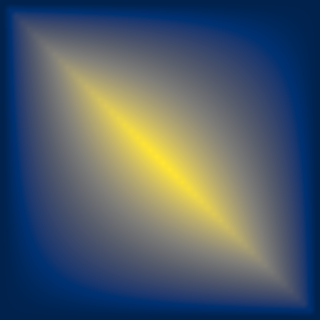
\includegraphics[interpolate=true,width=3.200000in,height=3.200000in]{figures/mccormick/mccormick-bounds-0-lower-img0.png}}%
\end{pgfscope}%
\begin{pgfscope}%
\pgfsetbuttcap%
\pgfsetroundjoin%
\definecolor{currentfill}{rgb}{0.000000,0.000000,0.000000}%
\pgfsetfillcolor{currentfill}%
\pgfsetlinewidth{0.803000pt}%
\definecolor{currentstroke}{rgb}{0.000000,0.000000,0.000000}%
\pgfsetstrokecolor{currentstroke}%
\pgfsetdash{}{0pt}%
\pgfsys@defobject{currentmarker}{\pgfqpoint{0.000000in}{-0.048611in}}{\pgfqpoint{0.000000in}{0.000000in}}{%
\pgfpathmoveto{\pgfqpoint{0.000000in}{0.000000in}}%
\pgfpathlineto{\pgfqpoint{0.000000in}{-0.048611in}}%
\pgfusepath{stroke,fill}%
}%
\begin{pgfscope}%
\pgfsys@transformshift{0.516434in}{0.499074in}%
\pgfsys@useobject{currentmarker}{}%
\end{pgfscope}%
\end{pgfscope}%
\begin{pgfscope}%
\definecolor{textcolor}{rgb}{0.000000,0.000000,0.000000}%
\pgfsetstrokecolor{textcolor}%
\pgfsetfillcolor{textcolor}%
\pgftext[x=0.516434in,y=0.401852in,,top]{\color{textcolor}{\rmfamily\fontsize{9.000000}{10.800000}\selectfont\catcode`\^=\active\def^{\ifmmode\sp\else\^{}\fi}\catcode`\%=\active\def%{\%}$\mathdefault{\ensuremath{-}2.0}$}}%
\end{pgfscope}%
\begin{pgfscope}%
\pgfsetbuttcap%
\pgfsetroundjoin%
\definecolor{currentfill}{rgb}{0.000000,0.000000,0.000000}%
\pgfsetfillcolor{currentfill}%
\pgfsetlinewidth{0.803000pt}%
\definecolor{currentstroke}{rgb}{0.000000,0.000000,0.000000}%
\pgfsetstrokecolor{currentstroke}%
\pgfsetdash{}{0pt}%
\pgfsys@defobject{currentmarker}{\pgfqpoint{0.000000in}{-0.048611in}}{\pgfqpoint{0.000000in}{0.000000in}}{%
\pgfpathmoveto{\pgfqpoint{0.000000in}{0.000000in}}%
\pgfpathlineto{\pgfqpoint{0.000000in}{-0.048611in}}%
\pgfusepath{stroke,fill}%
}%
\begin{pgfscope}%
\pgfsys@transformshift{0.916012in}{0.499074in}%
\pgfsys@useobject{currentmarker}{}%
\end{pgfscope}%
\end{pgfscope}%
\begin{pgfscope}%
\definecolor{textcolor}{rgb}{0.000000,0.000000,0.000000}%
\pgfsetstrokecolor{textcolor}%
\pgfsetfillcolor{textcolor}%
\pgftext[x=0.916012in,y=0.401852in,,top]{\color{textcolor}{\rmfamily\fontsize{9.000000}{10.800000}\selectfont\catcode`\^=\active\def^{\ifmmode\sp\else\^{}\fi}\catcode`\%=\active\def%{\%}$\mathdefault{\ensuremath{-}1.5}$}}%
\end{pgfscope}%
\begin{pgfscope}%
\pgfsetbuttcap%
\pgfsetroundjoin%
\definecolor{currentfill}{rgb}{0.000000,0.000000,0.000000}%
\pgfsetfillcolor{currentfill}%
\pgfsetlinewidth{0.803000pt}%
\definecolor{currentstroke}{rgb}{0.000000,0.000000,0.000000}%
\pgfsetstrokecolor{currentstroke}%
\pgfsetdash{}{0pt}%
\pgfsys@defobject{currentmarker}{\pgfqpoint{0.000000in}{-0.048611in}}{\pgfqpoint{0.000000in}{0.000000in}}{%
\pgfpathmoveto{\pgfqpoint{0.000000in}{0.000000in}}%
\pgfpathlineto{\pgfqpoint{0.000000in}{-0.048611in}}%
\pgfusepath{stroke,fill}%
}%
\begin{pgfscope}%
\pgfsys@transformshift{1.315591in}{0.499074in}%
\pgfsys@useobject{currentmarker}{}%
\end{pgfscope}%
\end{pgfscope}%
\begin{pgfscope}%
\definecolor{textcolor}{rgb}{0.000000,0.000000,0.000000}%
\pgfsetstrokecolor{textcolor}%
\pgfsetfillcolor{textcolor}%
\pgftext[x=1.315591in,y=0.401852in,,top]{\color{textcolor}{\rmfamily\fontsize{9.000000}{10.800000}\selectfont\catcode`\^=\active\def^{\ifmmode\sp\else\^{}\fi}\catcode`\%=\active\def%{\%}$\mathdefault{\ensuremath{-}1.0}$}}%
\end{pgfscope}%
\begin{pgfscope}%
\pgfsetbuttcap%
\pgfsetroundjoin%
\definecolor{currentfill}{rgb}{0.000000,0.000000,0.000000}%
\pgfsetfillcolor{currentfill}%
\pgfsetlinewidth{0.803000pt}%
\definecolor{currentstroke}{rgb}{0.000000,0.000000,0.000000}%
\pgfsetstrokecolor{currentstroke}%
\pgfsetdash{}{0pt}%
\pgfsys@defobject{currentmarker}{\pgfqpoint{0.000000in}{-0.048611in}}{\pgfqpoint{0.000000in}{0.000000in}}{%
\pgfpathmoveto{\pgfqpoint{0.000000in}{0.000000in}}%
\pgfpathlineto{\pgfqpoint{0.000000in}{-0.048611in}}%
\pgfusepath{stroke,fill}%
}%
\begin{pgfscope}%
\pgfsys@transformshift{1.715169in}{0.499074in}%
\pgfsys@useobject{currentmarker}{}%
\end{pgfscope}%
\end{pgfscope}%
\begin{pgfscope}%
\definecolor{textcolor}{rgb}{0.000000,0.000000,0.000000}%
\pgfsetstrokecolor{textcolor}%
\pgfsetfillcolor{textcolor}%
\pgftext[x=1.715169in,y=0.401852in,,top]{\color{textcolor}{\rmfamily\fontsize{9.000000}{10.800000}\selectfont\catcode`\^=\active\def^{\ifmmode\sp\else\^{}\fi}\catcode`\%=\active\def%{\%}$\mathdefault{\ensuremath{-}0.5}$}}%
\end{pgfscope}%
\begin{pgfscope}%
\pgfsetbuttcap%
\pgfsetroundjoin%
\definecolor{currentfill}{rgb}{0.000000,0.000000,0.000000}%
\pgfsetfillcolor{currentfill}%
\pgfsetlinewidth{0.803000pt}%
\definecolor{currentstroke}{rgb}{0.000000,0.000000,0.000000}%
\pgfsetstrokecolor{currentstroke}%
\pgfsetdash{}{0pt}%
\pgfsys@defobject{currentmarker}{\pgfqpoint{0.000000in}{-0.048611in}}{\pgfqpoint{0.000000in}{0.000000in}}{%
\pgfpathmoveto{\pgfqpoint{0.000000in}{0.000000in}}%
\pgfpathlineto{\pgfqpoint{0.000000in}{-0.048611in}}%
\pgfusepath{stroke,fill}%
}%
\begin{pgfscope}%
\pgfsys@transformshift{2.114747in}{0.499074in}%
\pgfsys@useobject{currentmarker}{}%
\end{pgfscope}%
\end{pgfscope}%
\begin{pgfscope}%
\definecolor{textcolor}{rgb}{0.000000,0.000000,0.000000}%
\pgfsetstrokecolor{textcolor}%
\pgfsetfillcolor{textcolor}%
\pgftext[x=2.114747in,y=0.401852in,,top]{\color{textcolor}{\rmfamily\fontsize{9.000000}{10.800000}\selectfont\catcode`\^=\active\def^{\ifmmode\sp\else\^{}\fi}\catcode`\%=\active\def%{\%}$\mathdefault{0.0}$}}%
\end{pgfscope}%
\begin{pgfscope}%
\pgfsetbuttcap%
\pgfsetroundjoin%
\definecolor{currentfill}{rgb}{0.000000,0.000000,0.000000}%
\pgfsetfillcolor{currentfill}%
\pgfsetlinewidth{0.803000pt}%
\definecolor{currentstroke}{rgb}{0.000000,0.000000,0.000000}%
\pgfsetstrokecolor{currentstroke}%
\pgfsetdash{}{0pt}%
\pgfsys@defobject{currentmarker}{\pgfqpoint{0.000000in}{-0.048611in}}{\pgfqpoint{0.000000in}{0.000000in}}{%
\pgfpathmoveto{\pgfqpoint{0.000000in}{0.000000in}}%
\pgfpathlineto{\pgfqpoint{0.000000in}{-0.048611in}}%
\pgfusepath{stroke,fill}%
}%
\begin{pgfscope}%
\pgfsys@transformshift{2.514325in}{0.499074in}%
\pgfsys@useobject{currentmarker}{}%
\end{pgfscope}%
\end{pgfscope}%
\begin{pgfscope}%
\definecolor{textcolor}{rgb}{0.000000,0.000000,0.000000}%
\pgfsetstrokecolor{textcolor}%
\pgfsetfillcolor{textcolor}%
\pgftext[x=2.514325in,y=0.401852in,,top]{\color{textcolor}{\rmfamily\fontsize{9.000000}{10.800000}\selectfont\catcode`\^=\active\def^{\ifmmode\sp\else\^{}\fi}\catcode`\%=\active\def%{\%}$\mathdefault{0.5}$}}%
\end{pgfscope}%
\begin{pgfscope}%
\pgfsetbuttcap%
\pgfsetroundjoin%
\definecolor{currentfill}{rgb}{0.000000,0.000000,0.000000}%
\pgfsetfillcolor{currentfill}%
\pgfsetlinewidth{0.803000pt}%
\definecolor{currentstroke}{rgb}{0.000000,0.000000,0.000000}%
\pgfsetstrokecolor{currentstroke}%
\pgfsetdash{}{0pt}%
\pgfsys@defobject{currentmarker}{\pgfqpoint{0.000000in}{-0.048611in}}{\pgfqpoint{0.000000in}{0.000000in}}{%
\pgfpathmoveto{\pgfqpoint{0.000000in}{0.000000in}}%
\pgfpathlineto{\pgfqpoint{0.000000in}{-0.048611in}}%
\pgfusepath{stroke,fill}%
}%
\begin{pgfscope}%
\pgfsys@transformshift{2.913903in}{0.499074in}%
\pgfsys@useobject{currentmarker}{}%
\end{pgfscope}%
\end{pgfscope}%
\begin{pgfscope}%
\definecolor{textcolor}{rgb}{0.000000,0.000000,0.000000}%
\pgfsetstrokecolor{textcolor}%
\pgfsetfillcolor{textcolor}%
\pgftext[x=2.913903in,y=0.401852in,,top]{\color{textcolor}{\rmfamily\fontsize{9.000000}{10.800000}\selectfont\catcode`\^=\active\def^{\ifmmode\sp\else\^{}\fi}\catcode`\%=\active\def%{\%}$\mathdefault{1.0}$}}%
\end{pgfscope}%
\begin{pgfscope}%
\pgfsetbuttcap%
\pgfsetroundjoin%
\definecolor{currentfill}{rgb}{0.000000,0.000000,0.000000}%
\pgfsetfillcolor{currentfill}%
\pgfsetlinewidth{0.803000pt}%
\definecolor{currentstroke}{rgb}{0.000000,0.000000,0.000000}%
\pgfsetstrokecolor{currentstroke}%
\pgfsetdash{}{0pt}%
\pgfsys@defobject{currentmarker}{\pgfqpoint{0.000000in}{-0.048611in}}{\pgfqpoint{0.000000in}{0.000000in}}{%
\pgfpathmoveto{\pgfqpoint{0.000000in}{0.000000in}}%
\pgfpathlineto{\pgfqpoint{0.000000in}{-0.048611in}}%
\pgfusepath{stroke,fill}%
}%
\begin{pgfscope}%
\pgfsys@transformshift{3.313482in}{0.499074in}%
\pgfsys@useobject{currentmarker}{}%
\end{pgfscope}%
\end{pgfscope}%
\begin{pgfscope}%
\definecolor{textcolor}{rgb}{0.000000,0.000000,0.000000}%
\pgfsetstrokecolor{textcolor}%
\pgfsetfillcolor{textcolor}%
\pgftext[x=3.313482in,y=0.401852in,,top]{\color{textcolor}{\rmfamily\fontsize{9.000000}{10.800000}\selectfont\catcode`\^=\active\def^{\ifmmode\sp\else\^{}\fi}\catcode`\%=\active\def%{\%}$\mathdefault{1.5}$}}%
\end{pgfscope}%
\begin{pgfscope}%
\pgfsetbuttcap%
\pgfsetroundjoin%
\definecolor{currentfill}{rgb}{0.000000,0.000000,0.000000}%
\pgfsetfillcolor{currentfill}%
\pgfsetlinewidth{0.803000pt}%
\definecolor{currentstroke}{rgb}{0.000000,0.000000,0.000000}%
\pgfsetstrokecolor{currentstroke}%
\pgfsetdash{}{0pt}%
\pgfsys@defobject{currentmarker}{\pgfqpoint{0.000000in}{-0.048611in}}{\pgfqpoint{0.000000in}{0.000000in}}{%
\pgfpathmoveto{\pgfqpoint{0.000000in}{0.000000in}}%
\pgfpathlineto{\pgfqpoint{0.000000in}{-0.048611in}}%
\pgfusepath{stroke,fill}%
}%
\begin{pgfscope}%
\pgfsys@transformshift{3.713060in}{0.499074in}%
\pgfsys@useobject{currentmarker}{}%
\end{pgfscope}%
\end{pgfscope}%
\begin{pgfscope}%
\definecolor{textcolor}{rgb}{0.000000,0.000000,0.000000}%
\pgfsetstrokecolor{textcolor}%
\pgfsetfillcolor{textcolor}%
\pgftext[x=3.713060in,y=0.401852in,,top]{\color{textcolor}{\rmfamily\fontsize{9.000000}{10.800000}\selectfont\catcode`\^=\active\def^{\ifmmode\sp\else\^{}\fi}\catcode`\%=\active\def%{\%}$\mathdefault{2.0}$}}%
\end{pgfscope}%
\begin{pgfscope}%
\definecolor{textcolor}{rgb}{0.000000,0.000000,0.000000}%
\pgfsetstrokecolor{textcolor}%
\pgfsetfillcolor{textcolor}%
\pgftext[x=2.114747in,y=0.235185in,,top]{\color{textcolor}{\rmfamily\fontsize{11.000000}{13.200000}\selectfont\catcode`\^=\active\def^{\ifmmode\sp\else\^{}\fi}\catcode`\%=\active\def%{\%}$v_1$}}%
\end{pgfscope}%
\begin{pgfscope}%
\pgfsetbuttcap%
\pgfsetroundjoin%
\definecolor{currentfill}{rgb}{0.000000,0.000000,0.000000}%
\pgfsetfillcolor{currentfill}%
\pgfsetlinewidth{0.803000pt}%
\definecolor{currentstroke}{rgb}{0.000000,0.000000,0.000000}%
\pgfsetstrokecolor{currentstroke}%
\pgfsetdash{}{0pt}%
\pgfsys@defobject{currentmarker}{\pgfqpoint{-0.048611in}{0.000000in}}{\pgfqpoint{-0.000000in}{0.000000in}}{%
\pgfpathmoveto{\pgfqpoint{-0.000000in}{0.000000in}}%
\pgfpathlineto{\pgfqpoint{-0.048611in}{0.000000in}}%
\pgfusepath{stroke,fill}%
}%
\begin{pgfscope}%
\pgfsys@transformshift{0.516434in}{0.499074in}%
\pgfsys@useobject{currentmarker}{}%
\end{pgfscope}%
\end{pgfscope}%
\begin{pgfscope}%
\definecolor{textcolor}{rgb}{0.000000,0.000000,0.000000}%
\pgfsetstrokecolor{textcolor}%
\pgfsetfillcolor{textcolor}%
\pgftext[x=0.354976in, y=0.455671in, left, base]{\color{textcolor}{\rmfamily\fontsize{9.000000}{10.800000}\selectfont\catcode`\^=\active\def^{\ifmmode\sp\else\^{}\fi}\catcode`\%=\active\def%{\%}$\mathdefault{0}$}}%
\end{pgfscope}%
\begin{pgfscope}%
\pgfsetbuttcap%
\pgfsetroundjoin%
\definecolor{currentfill}{rgb}{0.000000,0.000000,0.000000}%
\pgfsetfillcolor{currentfill}%
\pgfsetlinewidth{0.803000pt}%
\definecolor{currentstroke}{rgb}{0.000000,0.000000,0.000000}%
\pgfsetstrokecolor{currentstroke}%
\pgfsetdash{}{0pt}%
\pgfsys@defobject{currentmarker}{\pgfqpoint{-0.048611in}{0.000000in}}{\pgfqpoint{-0.000000in}{0.000000in}}{%
\pgfpathmoveto{\pgfqpoint{-0.000000in}{0.000000in}}%
\pgfpathlineto{\pgfqpoint{-0.048611in}{0.000000in}}%
\pgfusepath{stroke,fill}%
}%
\begin{pgfscope}%
\pgfsys@transformshift{0.516434in}{1.138399in}%
\pgfsys@useobject{currentmarker}{}%
\end{pgfscope}%
\end{pgfscope}%
\begin{pgfscope}%
\definecolor{textcolor}{rgb}{0.000000,0.000000,0.000000}%
\pgfsetstrokecolor{textcolor}%
\pgfsetfillcolor{textcolor}%
\pgftext[x=0.290741in, y=1.094996in, left, base]{\color{textcolor}{\rmfamily\fontsize{9.000000}{10.800000}\selectfont\catcode`\^=\active\def^{\ifmmode\sp\else\^{}\fi}\catcode`\%=\active\def%{\%}$\mathdefault{10}$}}%
\end{pgfscope}%
\begin{pgfscope}%
\pgfsetbuttcap%
\pgfsetroundjoin%
\definecolor{currentfill}{rgb}{0.000000,0.000000,0.000000}%
\pgfsetfillcolor{currentfill}%
\pgfsetlinewidth{0.803000pt}%
\definecolor{currentstroke}{rgb}{0.000000,0.000000,0.000000}%
\pgfsetstrokecolor{currentstroke}%
\pgfsetdash{}{0pt}%
\pgfsys@defobject{currentmarker}{\pgfqpoint{-0.048611in}{0.000000in}}{\pgfqpoint{-0.000000in}{0.000000in}}{%
\pgfpathmoveto{\pgfqpoint{-0.000000in}{0.000000in}}%
\pgfpathlineto{\pgfqpoint{-0.048611in}{0.000000in}}%
\pgfusepath{stroke,fill}%
}%
\begin{pgfscope}%
\pgfsys@transformshift{0.516434in}{1.777724in}%
\pgfsys@useobject{currentmarker}{}%
\end{pgfscope}%
\end{pgfscope}%
\begin{pgfscope}%
\definecolor{textcolor}{rgb}{0.000000,0.000000,0.000000}%
\pgfsetstrokecolor{textcolor}%
\pgfsetfillcolor{textcolor}%
\pgftext[x=0.290741in, y=1.734321in, left, base]{\color{textcolor}{\rmfamily\fontsize{9.000000}{10.800000}\selectfont\catcode`\^=\active\def^{\ifmmode\sp\else\^{}\fi}\catcode`\%=\active\def%{\%}$\mathdefault{20}$}}%
\end{pgfscope}%
\begin{pgfscope}%
\pgfsetbuttcap%
\pgfsetroundjoin%
\definecolor{currentfill}{rgb}{0.000000,0.000000,0.000000}%
\pgfsetfillcolor{currentfill}%
\pgfsetlinewidth{0.803000pt}%
\definecolor{currentstroke}{rgb}{0.000000,0.000000,0.000000}%
\pgfsetstrokecolor{currentstroke}%
\pgfsetdash{}{0pt}%
\pgfsys@defobject{currentmarker}{\pgfqpoint{-0.048611in}{0.000000in}}{\pgfqpoint{-0.000000in}{0.000000in}}{%
\pgfpathmoveto{\pgfqpoint{-0.000000in}{0.000000in}}%
\pgfpathlineto{\pgfqpoint{-0.048611in}{0.000000in}}%
\pgfusepath{stroke,fill}%
}%
\begin{pgfscope}%
\pgfsys@transformshift{0.516434in}{2.417049in}%
\pgfsys@useobject{currentmarker}{}%
\end{pgfscope}%
\end{pgfscope}%
\begin{pgfscope}%
\definecolor{textcolor}{rgb}{0.000000,0.000000,0.000000}%
\pgfsetstrokecolor{textcolor}%
\pgfsetfillcolor{textcolor}%
\pgftext[x=0.290741in, y=2.373646in, left, base]{\color{textcolor}{\rmfamily\fontsize{9.000000}{10.800000}\selectfont\catcode`\^=\active\def^{\ifmmode\sp\else\^{}\fi}\catcode`\%=\active\def%{\%}$\mathdefault{30}$}}%
\end{pgfscope}%
\begin{pgfscope}%
\pgfsetbuttcap%
\pgfsetroundjoin%
\definecolor{currentfill}{rgb}{0.000000,0.000000,0.000000}%
\pgfsetfillcolor{currentfill}%
\pgfsetlinewidth{0.803000pt}%
\definecolor{currentstroke}{rgb}{0.000000,0.000000,0.000000}%
\pgfsetstrokecolor{currentstroke}%
\pgfsetdash{}{0pt}%
\pgfsys@defobject{currentmarker}{\pgfqpoint{-0.048611in}{0.000000in}}{\pgfqpoint{-0.000000in}{0.000000in}}{%
\pgfpathmoveto{\pgfqpoint{-0.000000in}{0.000000in}}%
\pgfpathlineto{\pgfqpoint{-0.048611in}{0.000000in}}%
\pgfusepath{stroke,fill}%
}%
\begin{pgfscope}%
\pgfsys@transformshift{0.516434in}{3.056374in}%
\pgfsys@useobject{currentmarker}{}%
\end{pgfscope}%
\end{pgfscope}%
\begin{pgfscope}%
\definecolor{textcolor}{rgb}{0.000000,0.000000,0.000000}%
\pgfsetstrokecolor{textcolor}%
\pgfsetfillcolor{textcolor}%
\pgftext[x=0.290741in, y=3.012972in, left, base]{\color{textcolor}{\rmfamily\fontsize{9.000000}{10.800000}\selectfont\catcode`\^=\active\def^{\ifmmode\sp\else\^{}\fi}\catcode`\%=\active\def%{\%}$\mathdefault{40}$}}%
\end{pgfscope}%
\begin{pgfscope}%
\pgfsetbuttcap%
\pgfsetroundjoin%
\definecolor{currentfill}{rgb}{0.000000,0.000000,0.000000}%
\pgfsetfillcolor{currentfill}%
\pgfsetlinewidth{0.803000pt}%
\definecolor{currentstroke}{rgb}{0.000000,0.000000,0.000000}%
\pgfsetstrokecolor{currentstroke}%
\pgfsetdash{}{0pt}%
\pgfsys@defobject{currentmarker}{\pgfqpoint{-0.048611in}{0.000000in}}{\pgfqpoint{-0.000000in}{0.000000in}}{%
\pgfpathmoveto{\pgfqpoint{-0.000000in}{0.000000in}}%
\pgfpathlineto{\pgfqpoint{-0.048611in}{0.000000in}}%
\pgfusepath{stroke,fill}%
}%
\begin{pgfscope}%
\pgfsys@transformshift{0.516434in}{3.695699in}%
\pgfsys@useobject{currentmarker}{}%
\end{pgfscope}%
\end{pgfscope}%
\begin{pgfscope}%
\definecolor{textcolor}{rgb}{0.000000,0.000000,0.000000}%
\pgfsetstrokecolor{textcolor}%
\pgfsetfillcolor{textcolor}%
\pgftext[x=0.290741in, y=3.652297in, left, base]{\color{textcolor}{\rmfamily\fontsize{9.000000}{10.800000}\selectfont\catcode`\^=\active\def^{\ifmmode\sp\else\^{}\fi}\catcode`\%=\active\def%{\%}$\mathdefault{50}$}}%
\end{pgfscope}%
\begin{pgfscope}%
\definecolor{textcolor}{rgb}{0.000000,0.000000,0.000000}%
\pgfsetstrokecolor{textcolor}%
\pgfsetfillcolor{textcolor}%
\pgftext[x=0.235185in,y=2.097387in,,bottom,rotate=90.000000]{\color{textcolor}{\rmfamily\fontsize{11.000000}{13.200000}\selectfont\catcode`\^=\active\def^{\ifmmode\sp\else\^{}\fi}\catcode`\%=\active\def%{\%}$v_2$}}%
\end{pgfscope}%
\begin{pgfscope}%
\pgfsetrectcap%
\pgfsetmiterjoin%
\pgfsetlinewidth{0.803000pt}%
\definecolor{currentstroke}{rgb}{0.000000,0.000000,0.000000}%
\pgfsetstrokecolor{currentstroke}%
\pgfsetdash{}{0pt}%
\pgfpathmoveto{\pgfqpoint{0.516434in}{0.499074in}}%
\pgfpathlineto{\pgfqpoint{0.516434in}{3.695699in}}%
\pgfusepath{stroke}%
\end{pgfscope}%
\begin{pgfscope}%
\pgfsetrectcap%
\pgfsetmiterjoin%
\pgfsetlinewidth{0.803000pt}%
\definecolor{currentstroke}{rgb}{0.000000,0.000000,0.000000}%
\pgfsetstrokecolor{currentstroke}%
\pgfsetdash{}{0pt}%
\pgfpathmoveto{\pgfqpoint{3.713060in}{0.499074in}}%
\pgfpathlineto{\pgfqpoint{3.713060in}{3.695699in}}%
\pgfusepath{stroke}%
\end{pgfscope}%
\begin{pgfscope}%
\pgfsetrectcap%
\pgfsetmiterjoin%
\pgfsetlinewidth{0.803000pt}%
\definecolor{currentstroke}{rgb}{0.000000,0.000000,0.000000}%
\pgfsetstrokecolor{currentstroke}%
\pgfsetdash{}{0pt}%
\pgfpathmoveto{\pgfqpoint{0.516434in}{0.499074in}}%
\pgfpathlineto{\pgfqpoint{3.713060in}{0.499074in}}%
\pgfusepath{stroke}%
\end{pgfscope}%
\begin{pgfscope}%
\pgfsetrectcap%
\pgfsetmiterjoin%
\pgfsetlinewidth{0.803000pt}%
\definecolor{currentstroke}{rgb}{0.000000,0.000000,0.000000}%
\pgfsetstrokecolor{currentstroke}%
\pgfsetdash{}{0pt}%
\pgfpathmoveto{\pgfqpoint{0.516434in}{3.695699in}}%
\pgfpathlineto{\pgfqpoint{3.713060in}{3.695699in}}%
\pgfusepath{stroke}%
\end{pgfscope}%
\begin{pgfscope}%
\pgfsetbuttcap%
\pgfsetmiterjoin%
\definecolor{currentfill}{rgb}{1.000000,1.000000,1.000000}%
\pgfsetfillcolor{currentfill}%
\pgfsetlinewidth{0.000000pt}%
\definecolor{currentstroke}{rgb}{0.000000,0.000000,0.000000}%
\pgfsetstrokecolor{currentstroke}%
\pgfsetstrokeopacity{0.000000}%
\pgfsetdash{}{0pt}%
\pgfpathmoveto{\pgfqpoint{3.891959in}{0.499074in}}%
\pgfpathlineto{\pgfqpoint{4.051791in}{0.499074in}}%
\pgfpathlineto{\pgfqpoint{4.051791in}{3.695699in}}%
\pgfpathlineto{\pgfqpoint{3.891959in}{3.695699in}}%
\pgfpathlineto{\pgfqpoint{3.891959in}{0.499074in}}%
\pgfpathclose%
\pgfusepath{fill}%
\end{pgfscope}%
\begin{pgfscope}%
\pgfsys@transformshift{3.890000in}{0.509102in}%
\pgftext[left,bottom]{
\includegraphics[interpolate=true,width=0.160000in,height=3.200000in]{figures/mccormick/mccormick-bounds-0-lower-img1.png}}%
\end{pgfscope}%
\begin{pgfscope}%
\pgfsetbuttcap%
\pgfsetroundjoin%
\definecolor{currentfill}{rgb}{0.000000,0.000000,0.000000}%
\pgfsetfillcolor{currentfill}%
\pgfsetlinewidth{0.803000pt}%
\definecolor{currentstroke}{rgb}{0.000000,0.000000,0.000000}%
\pgfsetstrokecolor{currentstroke}%
\pgfsetdash{}{0pt}%
\pgfsys@defobject{currentmarker}{\pgfqpoint{0.000000in}{0.000000in}}{\pgfqpoint{0.048611in}{0.000000in}}{%
\pgfpathmoveto{\pgfqpoint{0.000000in}{0.000000in}}%
\pgfpathlineto{\pgfqpoint{0.048611in}{0.000000in}}%
\pgfusepath{stroke,fill}%
}%
\begin{pgfscope}%
\pgfsys@transformshift{4.051791in}{0.499074in}%
\pgfsys@useobject{currentmarker}{}%
\end{pgfscope}%
\end{pgfscope}%
\begin{pgfscope}%
\definecolor{textcolor}{rgb}{0.000000,0.000000,0.000000}%
\pgfsetstrokecolor{textcolor}%
\pgfsetfillcolor{textcolor}%
\pgftext[x=4.149013in, y=0.455671in, left, base]{\color{textcolor}{\rmfamily\fontsize{9.000000}{10.800000}\selectfont\catcode`\^=\active\def^{\ifmmode\sp\else\^{}\fi}\catcode`\%=\active\def%{\%}$\mathdefault{0}$}}%
\end{pgfscope}%
\begin{pgfscope}%
\pgfsetbuttcap%
\pgfsetroundjoin%
\definecolor{currentfill}{rgb}{0.000000,0.000000,0.000000}%
\pgfsetfillcolor{currentfill}%
\pgfsetlinewidth{0.803000pt}%
\definecolor{currentstroke}{rgb}{0.000000,0.000000,0.000000}%
\pgfsetstrokecolor{currentstroke}%
\pgfsetdash{}{0pt}%
\pgfsys@defobject{currentmarker}{\pgfqpoint{0.000000in}{0.000000in}}{\pgfqpoint{0.048611in}{0.000000in}}{%
\pgfpathmoveto{\pgfqpoint{0.000000in}{0.000000in}}%
\pgfpathlineto{\pgfqpoint{0.048611in}{0.000000in}}%
\pgfusepath{stroke,fill}%
}%
\begin{pgfscope}%
\pgfsys@transformshift{4.051791in}{1.138399in}%
\pgfsys@useobject{currentmarker}{}%
\end{pgfscope}%
\end{pgfscope}%
\begin{pgfscope}%
\definecolor{textcolor}{rgb}{0.000000,0.000000,0.000000}%
\pgfsetstrokecolor{textcolor}%
\pgfsetfillcolor{textcolor}%
\pgftext[x=4.149013in, y=1.094996in, left, base]{\color{textcolor}{\rmfamily\fontsize{9.000000}{10.800000}\selectfont\catcode`\^=\active\def^{\ifmmode\sp\else\^{}\fi}\catcode`\%=\active\def%{\%}$\mathdefault{10}$}}%
\end{pgfscope}%
\begin{pgfscope}%
\pgfsetbuttcap%
\pgfsetroundjoin%
\definecolor{currentfill}{rgb}{0.000000,0.000000,0.000000}%
\pgfsetfillcolor{currentfill}%
\pgfsetlinewidth{0.803000pt}%
\definecolor{currentstroke}{rgb}{0.000000,0.000000,0.000000}%
\pgfsetstrokecolor{currentstroke}%
\pgfsetdash{}{0pt}%
\pgfsys@defobject{currentmarker}{\pgfqpoint{0.000000in}{0.000000in}}{\pgfqpoint{0.048611in}{0.000000in}}{%
\pgfpathmoveto{\pgfqpoint{0.000000in}{0.000000in}}%
\pgfpathlineto{\pgfqpoint{0.048611in}{0.000000in}}%
\pgfusepath{stroke,fill}%
}%
\begin{pgfscope}%
\pgfsys@transformshift{4.051791in}{1.777724in}%
\pgfsys@useobject{currentmarker}{}%
\end{pgfscope}%
\end{pgfscope}%
\begin{pgfscope}%
\definecolor{textcolor}{rgb}{0.000000,0.000000,0.000000}%
\pgfsetstrokecolor{textcolor}%
\pgfsetfillcolor{textcolor}%
\pgftext[x=4.149013in, y=1.734321in, left, base]{\color{textcolor}{\rmfamily\fontsize{9.000000}{10.800000}\selectfont\catcode`\^=\active\def^{\ifmmode\sp\else\^{}\fi}\catcode`\%=\active\def%{\%}$\mathdefault{20}$}}%
\end{pgfscope}%
\begin{pgfscope}%
\pgfsetbuttcap%
\pgfsetroundjoin%
\definecolor{currentfill}{rgb}{0.000000,0.000000,0.000000}%
\pgfsetfillcolor{currentfill}%
\pgfsetlinewidth{0.803000pt}%
\definecolor{currentstroke}{rgb}{0.000000,0.000000,0.000000}%
\pgfsetstrokecolor{currentstroke}%
\pgfsetdash{}{0pt}%
\pgfsys@defobject{currentmarker}{\pgfqpoint{0.000000in}{0.000000in}}{\pgfqpoint{0.048611in}{0.000000in}}{%
\pgfpathmoveto{\pgfqpoint{0.000000in}{0.000000in}}%
\pgfpathlineto{\pgfqpoint{0.048611in}{0.000000in}}%
\pgfusepath{stroke,fill}%
}%
\begin{pgfscope}%
\pgfsys@transformshift{4.051791in}{2.417049in}%
\pgfsys@useobject{currentmarker}{}%
\end{pgfscope}%
\end{pgfscope}%
\begin{pgfscope}%
\definecolor{textcolor}{rgb}{0.000000,0.000000,0.000000}%
\pgfsetstrokecolor{textcolor}%
\pgfsetfillcolor{textcolor}%
\pgftext[x=4.149013in, y=2.373646in, left, base]{\color{textcolor}{\rmfamily\fontsize{9.000000}{10.800000}\selectfont\catcode`\^=\active\def^{\ifmmode\sp\else\^{}\fi}\catcode`\%=\active\def%{\%}$\mathdefault{30}$}}%
\end{pgfscope}%
\begin{pgfscope}%
\pgfsetbuttcap%
\pgfsetroundjoin%
\definecolor{currentfill}{rgb}{0.000000,0.000000,0.000000}%
\pgfsetfillcolor{currentfill}%
\pgfsetlinewidth{0.803000pt}%
\definecolor{currentstroke}{rgb}{0.000000,0.000000,0.000000}%
\pgfsetstrokecolor{currentstroke}%
\pgfsetdash{}{0pt}%
\pgfsys@defobject{currentmarker}{\pgfqpoint{0.000000in}{0.000000in}}{\pgfqpoint{0.048611in}{0.000000in}}{%
\pgfpathmoveto{\pgfqpoint{0.000000in}{0.000000in}}%
\pgfpathlineto{\pgfqpoint{0.048611in}{0.000000in}}%
\pgfusepath{stroke,fill}%
}%
\begin{pgfscope}%
\pgfsys@transformshift{4.051791in}{3.056374in}%
\pgfsys@useobject{currentmarker}{}%
\end{pgfscope}%
\end{pgfscope}%
\begin{pgfscope}%
\definecolor{textcolor}{rgb}{0.000000,0.000000,0.000000}%
\pgfsetstrokecolor{textcolor}%
\pgfsetfillcolor{textcolor}%
\pgftext[x=4.149013in, y=3.012972in, left, base]{\color{textcolor}{\rmfamily\fontsize{9.000000}{10.800000}\selectfont\catcode`\^=\active\def^{\ifmmode\sp\else\^{}\fi}\catcode`\%=\active\def%{\%}$\mathdefault{40}$}}%
\end{pgfscope}%
\begin{pgfscope}%
\pgfsetbuttcap%
\pgfsetroundjoin%
\definecolor{currentfill}{rgb}{0.000000,0.000000,0.000000}%
\pgfsetfillcolor{currentfill}%
\pgfsetlinewidth{0.803000pt}%
\definecolor{currentstroke}{rgb}{0.000000,0.000000,0.000000}%
\pgfsetstrokecolor{currentstroke}%
\pgfsetdash{}{0pt}%
\pgfsys@defobject{currentmarker}{\pgfqpoint{0.000000in}{0.000000in}}{\pgfqpoint{0.048611in}{0.000000in}}{%
\pgfpathmoveto{\pgfqpoint{0.000000in}{0.000000in}}%
\pgfpathlineto{\pgfqpoint{0.048611in}{0.000000in}}%
\pgfusepath{stroke,fill}%
}%
\begin{pgfscope}%
\pgfsys@transformshift{4.051791in}{3.695699in}%
\pgfsys@useobject{currentmarker}{}%
\end{pgfscope}%
\end{pgfscope}%
\begin{pgfscope}%
\definecolor{textcolor}{rgb}{0.000000,0.000000,0.000000}%
\pgfsetstrokecolor{textcolor}%
\pgfsetfillcolor{textcolor}%
\pgftext[x=4.149013in, y=3.652297in, left, base]{\color{textcolor}{\rmfamily\fontsize{9.000000}{10.800000}\selectfont\catcode`\^=\active\def^{\ifmmode\sp\else\^{}\fi}\catcode`\%=\active\def%{\%}$\mathdefault{50}$}}%
\end{pgfscope}%
\begin{pgfscope}%
\pgfsetrectcap%
\pgfsetmiterjoin%
\pgfsetlinewidth{0.803000pt}%
\definecolor{currentstroke}{rgb}{0.000000,0.000000,0.000000}%
\pgfsetstrokecolor{currentstroke}%
\pgfsetdash{}{0pt}%
\pgfpathmoveto{\pgfqpoint{3.891959in}{0.499074in}}%
\pgfpathlineto{\pgfqpoint{3.971875in}{0.499074in}}%
\pgfpathlineto{\pgfqpoint{4.051791in}{0.499074in}}%
\pgfpathlineto{\pgfqpoint{4.051791in}{3.695699in}}%
\pgfpathlineto{\pgfqpoint{3.971875in}{3.695699in}}%
\pgfpathlineto{\pgfqpoint{3.891959in}{3.695699in}}%
\pgfpathlineto{\pgfqpoint{3.891959in}{0.499074in}}%
\pgfpathclose%
\pgfusepath{stroke}%
\end{pgfscope}%
\end{pgfpicture}%
\makeatother%
\endgroup%
}
		\caption{Difference to the lower bound}
		\label{fig:mccormick_0_lower}
	\end{subfigure}
	\caption{McCormick relaxation bounds for the bilinear term $ v_1v_2 $.}
	\label{fig:mccormick_bounds_0}
\end{figure}

Figure \ref{fig:mccormick_0_upper} shows the difference to the upper bound, while Figure \ref{fig:mccormick_0_lower} shows the difference to the
lower bound for the range $ -2 \leq v_1 \leq 2 $ and $ 0 \leq v_2 \leq 50 $.
It is evident that the bounds become tighter than $ v_1 $ and $ v_2 $ approach their respective limits.

\begin{figure}[h!]
	\centering
	\begin{subfigure}[b]{0.45\textwidth}
		\centering
		\resizebox{\textwidth}{!}{%% Creator: Matplotlib, PGF backend
%%
%% To include the figure in your LaTeX document, write
%%   \input{<filename>.pgf}
%%
%% Make sure the required packages are loaded in your preamble
%%   \usepackage{pgf}
%%
%% Also ensure that all the required font packages are loaded; for instance,
%% the lmodern package is sometimes necessary when using math font.
%%   \usepackage{lmodern}
%%
%% Figures using additional raster images can only be included by \input if
%% they are in the same directory as the main LaTeX file. For loading figures
%% from other directories you can use the `import` package
%%   \usepackage{import}
%%
%% and then include the figures with
%%   \import{<path to file>}{<filename>.pgf}
%%
%% Matplotlib used the following preamble
%%   \def\mathdefault#1{#1}
%%   \everymath=\expandafter{\the\everymath\displaystyle}
%%   
%%   \ifdefined\pdftexversion\else  % non-pdftex case.
%%     \usepackage{fontspec}
%%   \fi
%%   \makeatletter\@ifpackageloaded{underscore}{}{\usepackage[strings]{underscore}}\makeatother
%%
\begingroup%
\makeatletter%
\begin{pgfpicture}%
\pgfpathrectangle{\pgfpointorigin}{\pgfqpoint{4.377484in}{3.839102in}}%
\pgfusepath{use as bounding box, clip}%
\begin{pgfscope}%
\pgfsetbuttcap%
\pgfsetmiterjoin%
\definecolor{currentfill}{rgb}{1.000000,1.000000,1.000000}%
\pgfsetfillcolor{currentfill}%
\pgfsetlinewidth{0.000000pt}%
\definecolor{currentstroke}{rgb}{1.000000,1.000000,1.000000}%
\pgfsetstrokecolor{currentstroke}%
\pgfsetdash{}{0pt}%
\pgfpathmoveto{\pgfqpoint{0.000000in}{0.000000in}}%
\pgfpathlineto{\pgfqpoint{4.377484in}{0.000000in}}%
\pgfpathlineto{\pgfqpoint{4.377484in}{3.839102in}}%
\pgfpathlineto{\pgfqpoint{0.000000in}{3.839102in}}%
\pgfpathlineto{\pgfqpoint{0.000000in}{0.000000in}}%
\pgfpathclose%
\pgfusepath{fill}%
\end{pgfscope}%
\begin{pgfscope}%
\pgfsetbuttcap%
\pgfsetmiterjoin%
\definecolor{currentfill}{rgb}{1.000000,1.000000,1.000000}%
\pgfsetfillcolor{currentfill}%
\pgfsetlinewidth{0.000000pt}%
\definecolor{currentstroke}{rgb}{0.000000,0.000000,0.000000}%
\pgfsetstrokecolor{currentstroke}%
\pgfsetstrokeopacity{0.000000}%
\pgfsetdash{}{0pt}%
\pgfpathmoveto{\pgfqpoint{0.516434in}{0.499074in}}%
\pgfpathlineto{\pgfqpoint{3.713060in}{0.499074in}}%
\pgfpathlineto{\pgfqpoint{3.713060in}{3.695699in}}%
\pgfpathlineto{\pgfqpoint{0.516434in}{3.695699in}}%
\pgfpathlineto{\pgfqpoint{0.516434in}{0.499074in}}%
\pgfpathclose%
\pgfusepath{fill}%
\end{pgfscope}%
\begin{pgfscope}%
\pgfpathrectangle{\pgfqpoint{0.516434in}{0.499074in}}{\pgfqpoint{3.196625in}{3.196625in}}%
\pgfusepath{clip}%
\pgfsys@transformshift{0.516434in}{0.499074in}%
\pgftext[left,bottom]{
\includegraphics[interpolate=true,width=3.200000in,height=3.200000in]{figures/mccormick/mccormick-bounds-1-upper-img0.png}}%
\end{pgfscope}%
\begin{pgfscope}%
\pgfsetbuttcap%
\pgfsetroundjoin%
\definecolor{currentfill}{rgb}{0.000000,0.000000,0.000000}%
\pgfsetfillcolor{currentfill}%
\pgfsetlinewidth{0.803000pt}%
\definecolor{currentstroke}{rgb}{0.000000,0.000000,0.000000}%
\pgfsetstrokecolor{currentstroke}%
\pgfsetdash{}{0pt}%
\pgfsys@defobject{currentmarker}{\pgfqpoint{0.000000in}{-0.048611in}}{\pgfqpoint{0.000000in}{0.000000in}}{%
\pgfpathmoveto{\pgfqpoint{0.000000in}{0.000000in}}%
\pgfpathlineto{\pgfqpoint{0.000000in}{-0.048611in}}%
\pgfusepath{stroke,fill}%
}%
\begin{pgfscope}%
\pgfsys@transformshift{0.516434in}{0.499074in}%
\pgfsys@useobject{currentmarker}{}%
\end{pgfscope}%
\end{pgfscope}%
\begin{pgfscope}%
\definecolor{textcolor}{rgb}{0.000000,0.000000,0.000000}%
\pgfsetstrokecolor{textcolor}%
\pgfsetfillcolor{textcolor}%
\pgftext[x=0.516434in,y=0.401852in,,top]{\color{textcolor}{\rmfamily\fontsize{9.000000}{10.800000}\selectfont\catcode`\^=\active\def^{\ifmmode\sp\else\^{}\fi}\catcode`\%=\active\def%{\%}$\mathdefault{\ensuremath{-}2.00}$}}%
\end{pgfscope}%
\begin{pgfscope}%
\pgfsetbuttcap%
\pgfsetroundjoin%
\definecolor{currentfill}{rgb}{0.000000,0.000000,0.000000}%
\pgfsetfillcolor{currentfill}%
\pgfsetlinewidth{0.803000pt}%
\definecolor{currentstroke}{rgb}{0.000000,0.000000,0.000000}%
\pgfsetstrokecolor{currentstroke}%
\pgfsetdash{}{0pt}%
\pgfsys@defobject{currentmarker}{\pgfqpoint{0.000000in}{-0.048611in}}{\pgfqpoint{0.000000in}{0.000000in}}{%
\pgfpathmoveto{\pgfqpoint{0.000000in}{0.000000in}}%
\pgfpathlineto{\pgfqpoint{0.000000in}{-0.048611in}}%
\pgfusepath{stroke,fill}%
}%
\begin{pgfscope}%
\pgfsys@transformshift{0.916012in}{0.499074in}%
\pgfsys@useobject{currentmarker}{}%
\end{pgfscope}%
\end{pgfscope}%
\begin{pgfscope}%
\definecolor{textcolor}{rgb}{0.000000,0.000000,0.000000}%
\pgfsetstrokecolor{textcolor}%
\pgfsetfillcolor{textcolor}%
\pgftext[x=0.916012in,y=0.401852in,,top]{\color{textcolor}{\rmfamily\fontsize{9.000000}{10.800000}\selectfont\catcode`\^=\active\def^{\ifmmode\sp\else\^{}\fi}\catcode`\%=\active\def%{\%}$\mathdefault{\ensuremath{-}1.75}$}}%
\end{pgfscope}%
\begin{pgfscope}%
\pgfsetbuttcap%
\pgfsetroundjoin%
\definecolor{currentfill}{rgb}{0.000000,0.000000,0.000000}%
\pgfsetfillcolor{currentfill}%
\pgfsetlinewidth{0.803000pt}%
\definecolor{currentstroke}{rgb}{0.000000,0.000000,0.000000}%
\pgfsetstrokecolor{currentstroke}%
\pgfsetdash{}{0pt}%
\pgfsys@defobject{currentmarker}{\pgfqpoint{0.000000in}{-0.048611in}}{\pgfqpoint{0.000000in}{0.000000in}}{%
\pgfpathmoveto{\pgfqpoint{0.000000in}{0.000000in}}%
\pgfpathlineto{\pgfqpoint{0.000000in}{-0.048611in}}%
\pgfusepath{stroke,fill}%
}%
\begin{pgfscope}%
\pgfsys@transformshift{1.315591in}{0.499074in}%
\pgfsys@useobject{currentmarker}{}%
\end{pgfscope}%
\end{pgfscope}%
\begin{pgfscope}%
\definecolor{textcolor}{rgb}{0.000000,0.000000,0.000000}%
\pgfsetstrokecolor{textcolor}%
\pgfsetfillcolor{textcolor}%
\pgftext[x=1.315591in,y=0.401852in,,top]{\color{textcolor}{\rmfamily\fontsize{9.000000}{10.800000}\selectfont\catcode`\^=\active\def^{\ifmmode\sp\else\^{}\fi}\catcode`\%=\active\def%{\%}$\mathdefault{\ensuremath{-}1.50}$}}%
\end{pgfscope}%
\begin{pgfscope}%
\pgfsetbuttcap%
\pgfsetroundjoin%
\definecolor{currentfill}{rgb}{0.000000,0.000000,0.000000}%
\pgfsetfillcolor{currentfill}%
\pgfsetlinewidth{0.803000pt}%
\definecolor{currentstroke}{rgb}{0.000000,0.000000,0.000000}%
\pgfsetstrokecolor{currentstroke}%
\pgfsetdash{}{0pt}%
\pgfsys@defobject{currentmarker}{\pgfqpoint{0.000000in}{-0.048611in}}{\pgfqpoint{0.000000in}{0.000000in}}{%
\pgfpathmoveto{\pgfqpoint{0.000000in}{0.000000in}}%
\pgfpathlineto{\pgfqpoint{0.000000in}{-0.048611in}}%
\pgfusepath{stroke,fill}%
}%
\begin{pgfscope}%
\pgfsys@transformshift{1.715169in}{0.499074in}%
\pgfsys@useobject{currentmarker}{}%
\end{pgfscope}%
\end{pgfscope}%
\begin{pgfscope}%
\definecolor{textcolor}{rgb}{0.000000,0.000000,0.000000}%
\pgfsetstrokecolor{textcolor}%
\pgfsetfillcolor{textcolor}%
\pgftext[x=1.715169in,y=0.401852in,,top]{\color{textcolor}{\rmfamily\fontsize{9.000000}{10.800000}\selectfont\catcode`\^=\active\def^{\ifmmode\sp\else\^{}\fi}\catcode`\%=\active\def%{\%}$\mathdefault{\ensuremath{-}1.25}$}}%
\end{pgfscope}%
\begin{pgfscope}%
\pgfsetbuttcap%
\pgfsetroundjoin%
\definecolor{currentfill}{rgb}{0.000000,0.000000,0.000000}%
\pgfsetfillcolor{currentfill}%
\pgfsetlinewidth{0.803000pt}%
\definecolor{currentstroke}{rgb}{0.000000,0.000000,0.000000}%
\pgfsetstrokecolor{currentstroke}%
\pgfsetdash{}{0pt}%
\pgfsys@defobject{currentmarker}{\pgfqpoint{0.000000in}{-0.048611in}}{\pgfqpoint{0.000000in}{0.000000in}}{%
\pgfpathmoveto{\pgfqpoint{0.000000in}{0.000000in}}%
\pgfpathlineto{\pgfqpoint{0.000000in}{-0.048611in}}%
\pgfusepath{stroke,fill}%
}%
\begin{pgfscope}%
\pgfsys@transformshift{2.114747in}{0.499074in}%
\pgfsys@useobject{currentmarker}{}%
\end{pgfscope}%
\end{pgfscope}%
\begin{pgfscope}%
\definecolor{textcolor}{rgb}{0.000000,0.000000,0.000000}%
\pgfsetstrokecolor{textcolor}%
\pgfsetfillcolor{textcolor}%
\pgftext[x=2.114747in,y=0.401852in,,top]{\color{textcolor}{\rmfamily\fontsize{9.000000}{10.800000}\selectfont\catcode`\^=\active\def^{\ifmmode\sp\else\^{}\fi}\catcode`\%=\active\def%{\%}$\mathdefault{\ensuremath{-}1.00}$}}%
\end{pgfscope}%
\begin{pgfscope}%
\pgfsetbuttcap%
\pgfsetroundjoin%
\definecolor{currentfill}{rgb}{0.000000,0.000000,0.000000}%
\pgfsetfillcolor{currentfill}%
\pgfsetlinewidth{0.803000pt}%
\definecolor{currentstroke}{rgb}{0.000000,0.000000,0.000000}%
\pgfsetstrokecolor{currentstroke}%
\pgfsetdash{}{0pt}%
\pgfsys@defobject{currentmarker}{\pgfqpoint{0.000000in}{-0.048611in}}{\pgfqpoint{0.000000in}{0.000000in}}{%
\pgfpathmoveto{\pgfqpoint{0.000000in}{0.000000in}}%
\pgfpathlineto{\pgfqpoint{0.000000in}{-0.048611in}}%
\pgfusepath{stroke,fill}%
}%
\begin{pgfscope}%
\pgfsys@transformshift{2.514325in}{0.499074in}%
\pgfsys@useobject{currentmarker}{}%
\end{pgfscope}%
\end{pgfscope}%
\begin{pgfscope}%
\definecolor{textcolor}{rgb}{0.000000,0.000000,0.000000}%
\pgfsetstrokecolor{textcolor}%
\pgfsetfillcolor{textcolor}%
\pgftext[x=2.514325in,y=0.401852in,,top]{\color{textcolor}{\rmfamily\fontsize{9.000000}{10.800000}\selectfont\catcode`\^=\active\def^{\ifmmode\sp\else\^{}\fi}\catcode`\%=\active\def%{\%}$\mathdefault{\ensuremath{-}0.75}$}}%
\end{pgfscope}%
\begin{pgfscope}%
\pgfsetbuttcap%
\pgfsetroundjoin%
\definecolor{currentfill}{rgb}{0.000000,0.000000,0.000000}%
\pgfsetfillcolor{currentfill}%
\pgfsetlinewidth{0.803000pt}%
\definecolor{currentstroke}{rgb}{0.000000,0.000000,0.000000}%
\pgfsetstrokecolor{currentstroke}%
\pgfsetdash{}{0pt}%
\pgfsys@defobject{currentmarker}{\pgfqpoint{0.000000in}{-0.048611in}}{\pgfqpoint{0.000000in}{0.000000in}}{%
\pgfpathmoveto{\pgfqpoint{0.000000in}{0.000000in}}%
\pgfpathlineto{\pgfqpoint{0.000000in}{-0.048611in}}%
\pgfusepath{stroke,fill}%
}%
\begin{pgfscope}%
\pgfsys@transformshift{2.913903in}{0.499074in}%
\pgfsys@useobject{currentmarker}{}%
\end{pgfscope}%
\end{pgfscope}%
\begin{pgfscope}%
\definecolor{textcolor}{rgb}{0.000000,0.000000,0.000000}%
\pgfsetstrokecolor{textcolor}%
\pgfsetfillcolor{textcolor}%
\pgftext[x=2.913903in,y=0.401852in,,top]{\color{textcolor}{\rmfamily\fontsize{9.000000}{10.800000}\selectfont\catcode`\^=\active\def^{\ifmmode\sp\else\^{}\fi}\catcode`\%=\active\def%{\%}$\mathdefault{\ensuremath{-}0.50}$}}%
\end{pgfscope}%
\begin{pgfscope}%
\pgfsetbuttcap%
\pgfsetroundjoin%
\definecolor{currentfill}{rgb}{0.000000,0.000000,0.000000}%
\pgfsetfillcolor{currentfill}%
\pgfsetlinewidth{0.803000pt}%
\definecolor{currentstroke}{rgb}{0.000000,0.000000,0.000000}%
\pgfsetstrokecolor{currentstroke}%
\pgfsetdash{}{0pt}%
\pgfsys@defobject{currentmarker}{\pgfqpoint{0.000000in}{-0.048611in}}{\pgfqpoint{0.000000in}{0.000000in}}{%
\pgfpathmoveto{\pgfqpoint{0.000000in}{0.000000in}}%
\pgfpathlineto{\pgfqpoint{0.000000in}{-0.048611in}}%
\pgfusepath{stroke,fill}%
}%
\begin{pgfscope}%
\pgfsys@transformshift{3.313482in}{0.499074in}%
\pgfsys@useobject{currentmarker}{}%
\end{pgfscope}%
\end{pgfscope}%
\begin{pgfscope}%
\definecolor{textcolor}{rgb}{0.000000,0.000000,0.000000}%
\pgfsetstrokecolor{textcolor}%
\pgfsetfillcolor{textcolor}%
\pgftext[x=3.313482in,y=0.401852in,,top]{\color{textcolor}{\rmfamily\fontsize{9.000000}{10.800000}\selectfont\catcode`\^=\active\def^{\ifmmode\sp\else\^{}\fi}\catcode`\%=\active\def%{\%}$\mathdefault{\ensuremath{-}0.25}$}}%
\end{pgfscope}%
\begin{pgfscope}%
\pgfsetbuttcap%
\pgfsetroundjoin%
\definecolor{currentfill}{rgb}{0.000000,0.000000,0.000000}%
\pgfsetfillcolor{currentfill}%
\pgfsetlinewidth{0.803000pt}%
\definecolor{currentstroke}{rgb}{0.000000,0.000000,0.000000}%
\pgfsetstrokecolor{currentstroke}%
\pgfsetdash{}{0pt}%
\pgfsys@defobject{currentmarker}{\pgfqpoint{0.000000in}{-0.048611in}}{\pgfqpoint{0.000000in}{0.000000in}}{%
\pgfpathmoveto{\pgfqpoint{0.000000in}{0.000000in}}%
\pgfpathlineto{\pgfqpoint{0.000000in}{-0.048611in}}%
\pgfusepath{stroke,fill}%
}%
\begin{pgfscope}%
\pgfsys@transformshift{3.713060in}{0.499074in}%
\pgfsys@useobject{currentmarker}{}%
\end{pgfscope}%
\end{pgfscope}%
\begin{pgfscope}%
\definecolor{textcolor}{rgb}{0.000000,0.000000,0.000000}%
\pgfsetstrokecolor{textcolor}%
\pgfsetfillcolor{textcolor}%
\pgftext[x=3.713060in,y=0.401852in,,top]{\color{textcolor}{\rmfamily\fontsize{9.000000}{10.800000}\selectfont\catcode`\^=\active\def^{\ifmmode\sp\else\^{}\fi}\catcode`\%=\active\def%{\%}$\mathdefault{0.00}$}}%
\end{pgfscope}%
\begin{pgfscope}%
\definecolor{textcolor}{rgb}{0.000000,0.000000,0.000000}%
\pgfsetstrokecolor{textcolor}%
\pgfsetfillcolor{textcolor}%
\pgftext[x=2.114747in,y=0.235185in,,top]{\color{textcolor}{\rmfamily\fontsize{11.000000}{13.200000}\selectfont\catcode`\^=\active\def^{\ifmmode\sp\else\^{}\fi}\catcode`\%=\active\def%{\%}x}}%
\end{pgfscope}%
\begin{pgfscope}%
\pgfsetbuttcap%
\pgfsetroundjoin%
\definecolor{currentfill}{rgb}{0.000000,0.000000,0.000000}%
\pgfsetfillcolor{currentfill}%
\pgfsetlinewidth{0.803000pt}%
\definecolor{currentstroke}{rgb}{0.000000,0.000000,0.000000}%
\pgfsetstrokecolor{currentstroke}%
\pgfsetdash{}{0pt}%
\pgfsys@defobject{currentmarker}{\pgfqpoint{-0.048611in}{0.000000in}}{\pgfqpoint{-0.000000in}{0.000000in}}{%
\pgfpathmoveto{\pgfqpoint{-0.000000in}{0.000000in}}%
\pgfpathlineto{\pgfqpoint{-0.048611in}{0.000000in}}%
\pgfusepath{stroke,fill}%
}%
\begin{pgfscope}%
\pgfsys@transformshift{0.516434in}{0.499074in}%
\pgfsys@useobject{currentmarker}{}%
\end{pgfscope}%
\end{pgfscope}%
\begin{pgfscope}%
\definecolor{textcolor}{rgb}{0.000000,0.000000,0.000000}%
\pgfsetstrokecolor{textcolor}%
\pgfsetfillcolor{textcolor}%
\pgftext[x=0.354976in, y=0.455671in, left, base]{\color{textcolor}{\rmfamily\fontsize{9.000000}{10.800000}\selectfont\catcode`\^=\active\def^{\ifmmode\sp\else\^{}\fi}\catcode`\%=\active\def%{\%}$\mathdefault{0}$}}%
\end{pgfscope}%
\begin{pgfscope}%
\pgfsetbuttcap%
\pgfsetroundjoin%
\definecolor{currentfill}{rgb}{0.000000,0.000000,0.000000}%
\pgfsetfillcolor{currentfill}%
\pgfsetlinewidth{0.803000pt}%
\definecolor{currentstroke}{rgb}{0.000000,0.000000,0.000000}%
\pgfsetstrokecolor{currentstroke}%
\pgfsetdash{}{0pt}%
\pgfsys@defobject{currentmarker}{\pgfqpoint{-0.048611in}{0.000000in}}{\pgfqpoint{-0.000000in}{0.000000in}}{%
\pgfpathmoveto{\pgfqpoint{-0.000000in}{0.000000in}}%
\pgfpathlineto{\pgfqpoint{-0.048611in}{0.000000in}}%
\pgfusepath{stroke,fill}%
}%
\begin{pgfscope}%
\pgfsys@transformshift{0.516434in}{1.138399in}%
\pgfsys@useobject{currentmarker}{}%
\end{pgfscope}%
\end{pgfscope}%
\begin{pgfscope}%
\definecolor{textcolor}{rgb}{0.000000,0.000000,0.000000}%
\pgfsetstrokecolor{textcolor}%
\pgfsetfillcolor{textcolor}%
\pgftext[x=0.290741in, y=1.094996in, left, base]{\color{textcolor}{\rmfamily\fontsize{9.000000}{10.800000}\selectfont\catcode`\^=\active\def^{\ifmmode\sp\else\^{}\fi}\catcode`\%=\active\def%{\%}$\mathdefault{10}$}}%
\end{pgfscope}%
\begin{pgfscope}%
\pgfsetbuttcap%
\pgfsetroundjoin%
\definecolor{currentfill}{rgb}{0.000000,0.000000,0.000000}%
\pgfsetfillcolor{currentfill}%
\pgfsetlinewidth{0.803000pt}%
\definecolor{currentstroke}{rgb}{0.000000,0.000000,0.000000}%
\pgfsetstrokecolor{currentstroke}%
\pgfsetdash{}{0pt}%
\pgfsys@defobject{currentmarker}{\pgfqpoint{-0.048611in}{0.000000in}}{\pgfqpoint{-0.000000in}{0.000000in}}{%
\pgfpathmoveto{\pgfqpoint{-0.000000in}{0.000000in}}%
\pgfpathlineto{\pgfqpoint{-0.048611in}{0.000000in}}%
\pgfusepath{stroke,fill}%
}%
\begin{pgfscope}%
\pgfsys@transformshift{0.516434in}{1.777724in}%
\pgfsys@useobject{currentmarker}{}%
\end{pgfscope}%
\end{pgfscope}%
\begin{pgfscope}%
\definecolor{textcolor}{rgb}{0.000000,0.000000,0.000000}%
\pgfsetstrokecolor{textcolor}%
\pgfsetfillcolor{textcolor}%
\pgftext[x=0.290741in, y=1.734321in, left, base]{\color{textcolor}{\rmfamily\fontsize{9.000000}{10.800000}\selectfont\catcode`\^=\active\def^{\ifmmode\sp\else\^{}\fi}\catcode`\%=\active\def%{\%}$\mathdefault{20}$}}%
\end{pgfscope}%
\begin{pgfscope}%
\pgfsetbuttcap%
\pgfsetroundjoin%
\definecolor{currentfill}{rgb}{0.000000,0.000000,0.000000}%
\pgfsetfillcolor{currentfill}%
\pgfsetlinewidth{0.803000pt}%
\definecolor{currentstroke}{rgb}{0.000000,0.000000,0.000000}%
\pgfsetstrokecolor{currentstroke}%
\pgfsetdash{}{0pt}%
\pgfsys@defobject{currentmarker}{\pgfqpoint{-0.048611in}{0.000000in}}{\pgfqpoint{-0.000000in}{0.000000in}}{%
\pgfpathmoveto{\pgfqpoint{-0.000000in}{0.000000in}}%
\pgfpathlineto{\pgfqpoint{-0.048611in}{0.000000in}}%
\pgfusepath{stroke,fill}%
}%
\begin{pgfscope}%
\pgfsys@transformshift{0.516434in}{2.417049in}%
\pgfsys@useobject{currentmarker}{}%
\end{pgfscope}%
\end{pgfscope}%
\begin{pgfscope}%
\definecolor{textcolor}{rgb}{0.000000,0.000000,0.000000}%
\pgfsetstrokecolor{textcolor}%
\pgfsetfillcolor{textcolor}%
\pgftext[x=0.290741in, y=2.373646in, left, base]{\color{textcolor}{\rmfamily\fontsize{9.000000}{10.800000}\selectfont\catcode`\^=\active\def^{\ifmmode\sp\else\^{}\fi}\catcode`\%=\active\def%{\%}$\mathdefault{30}$}}%
\end{pgfscope}%
\begin{pgfscope}%
\pgfsetbuttcap%
\pgfsetroundjoin%
\definecolor{currentfill}{rgb}{0.000000,0.000000,0.000000}%
\pgfsetfillcolor{currentfill}%
\pgfsetlinewidth{0.803000pt}%
\definecolor{currentstroke}{rgb}{0.000000,0.000000,0.000000}%
\pgfsetstrokecolor{currentstroke}%
\pgfsetdash{}{0pt}%
\pgfsys@defobject{currentmarker}{\pgfqpoint{-0.048611in}{0.000000in}}{\pgfqpoint{-0.000000in}{0.000000in}}{%
\pgfpathmoveto{\pgfqpoint{-0.000000in}{0.000000in}}%
\pgfpathlineto{\pgfqpoint{-0.048611in}{0.000000in}}%
\pgfusepath{stroke,fill}%
}%
\begin{pgfscope}%
\pgfsys@transformshift{0.516434in}{3.056374in}%
\pgfsys@useobject{currentmarker}{}%
\end{pgfscope}%
\end{pgfscope}%
\begin{pgfscope}%
\definecolor{textcolor}{rgb}{0.000000,0.000000,0.000000}%
\pgfsetstrokecolor{textcolor}%
\pgfsetfillcolor{textcolor}%
\pgftext[x=0.290741in, y=3.012972in, left, base]{\color{textcolor}{\rmfamily\fontsize{9.000000}{10.800000}\selectfont\catcode`\^=\active\def^{\ifmmode\sp\else\^{}\fi}\catcode`\%=\active\def%{\%}$\mathdefault{40}$}}%
\end{pgfscope}%
\begin{pgfscope}%
\pgfsetbuttcap%
\pgfsetroundjoin%
\definecolor{currentfill}{rgb}{0.000000,0.000000,0.000000}%
\pgfsetfillcolor{currentfill}%
\pgfsetlinewidth{0.803000pt}%
\definecolor{currentstroke}{rgb}{0.000000,0.000000,0.000000}%
\pgfsetstrokecolor{currentstroke}%
\pgfsetdash{}{0pt}%
\pgfsys@defobject{currentmarker}{\pgfqpoint{-0.048611in}{0.000000in}}{\pgfqpoint{-0.000000in}{0.000000in}}{%
\pgfpathmoveto{\pgfqpoint{-0.000000in}{0.000000in}}%
\pgfpathlineto{\pgfqpoint{-0.048611in}{0.000000in}}%
\pgfusepath{stroke,fill}%
}%
\begin{pgfscope}%
\pgfsys@transformshift{0.516434in}{3.695699in}%
\pgfsys@useobject{currentmarker}{}%
\end{pgfscope}%
\end{pgfscope}%
\begin{pgfscope}%
\definecolor{textcolor}{rgb}{0.000000,0.000000,0.000000}%
\pgfsetstrokecolor{textcolor}%
\pgfsetfillcolor{textcolor}%
\pgftext[x=0.290741in, y=3.652297in, left, base]{\color{textcolor}{\rmfamily\fontsize{9.000000}{10.800000}\selectfont\catcode`\^=\active\def^{\ifmmode\sp\else\^{}\fi}\catcode`\%=\active\def%{\%}$\mathdefault{50}$}}%
\end{pgfscope}%
\begin{pgfscope}%
\definecolor{textcolor}{rgb}{0.000000,0.000000,0.000000}%
\pgfsetstrokecolor{textcolor}%
\pgfsetfillcolor{textcolor}%
\pgftext[x=0.235185in,y=2.097387in,,bottom,rotate=90.000000]{\color{textcolor}{\rmfamily\fontsize{11.000000}{13.200000}\selectfont\catcode`\^=\active\def^{\ifmmode\sp\else\^{}\fi}\catcode`\%=\active\def%{\%}y}}%
\end{pgfscope}%
\begin{pgfscope}%
\pgfsetrectcap%
\pgfsetmiterjoin%
\pgfsetlinewidth{0.803000pt}%
\definecolor{currentstroke}{rgb}{0.000000,0.000000,0.000000}%
\pgfsetstrokecolor{currentstroke}%
\pgfsetdash{}{0pt}%
\pgfpathmoveto{\pgfqpoint{0.516434in}{0.499074in}}%
\pgfpathlineto{\pgfqpoint{0.516434in}{3.695699in}}%
\pgfusepath{stroke}%
\end{pgfscope}%
\begin{pgfscope}%
\pgfsetrectcap%
\pgfsetmiterjoin%
\pgfsetlinewidth{0.803000pt}%
\definecolor{currentstroke}{rgb}{0.000000,0.000000,0.000000}%
\pgfsetstrokecolor{currentstroke}%
\pgfsetdash{}{0pt}%
\pgfpathmoveto{\pgfqpoint{3.713060in}{0.499074in}}%
\pgfpathlineto{\pgfqpoint{3.713060in}{3.695699in}}%
\pgfusepath{stroke}%
\end{pgfscope}%
\begin{pgfscope}%
\pgfsetrectcap%
\pgfsetmiterjoin%
\pgfsetlinewidth{0.803000pt}%
\definecolor{currentstroke}{rgb}{0.000000,0.000000,0.000000}%
\pgfsetstrokecolor{currentstroke}%
\pgfsetdash{}{0pt}%
\pgfpathmoveto{\pgfqpoint{0.516434in}{0.499074in}}%
\pgfpathlineto{\pgfqpoint{3.713060in}{0.499074in}}%
\pgfusepath{stroke}%
\end{pgfscope}%
\begin{pgfscope}%
\pgfsetrectcap%
\pgfsetmiterjoin%
\pgfsetlinewidth{0.803000pt}%
\definecolor{currentstroke}{rgb}{0.000000,0.000000,0.000000}%
\pgfsetstrokecolor{currentstroke}%
\pgfsetdash{}{0pt}%
\pgfpathmoveto{\pgfqpoint{0.516434in}{3.695699in}}%
\pgfpathlineto{\pgfqpoint{3.713060in}{3.695699in}}%
\pgfusepath{stroke}%
\end{pgfscope}%
\begin{pgfscope}%
\pgfsetbuttcap%
\pgfsetmiterjoin%
\definecolor{currentfill}{rgb}{1.000000,1.000000,1.000000}%
\pgfsetfillcolor{currentfill}%
\pgfsetlinewidth{0.000000pt}%
\definecolor{currentstroke}{rgb}{0.000000,0.000000,0.000000}%
\pgfsetstrokecolor{currentstroke}%
\pgfsetstrokeopacity{0.000000}%
\pgfsetdash{}{0pt}%
\pgfpathmoveto{\pgfqpoint{3.891959in}{0.499074in}}%
\pgfpathlineto{\pgfqpoint{4.051791in}{0.499074in}}%
\pgfpathlineto{\pgfqpoint{4.051791in}{3.695699in}}%
\pgfpathlineto{\pgfqpoint{3.891959in}{3.695699in}}%
\pgfpathlineto{\pgfqpoint{3.891959in}{0.499074in}}%
\pgfpathclose%
\pgfusepath{fill}%
\end{pgfscope}%
\begin{pgfscope}%
\pgfsys@transformshift{3.890000in}{0.509102in}%
\pgftext[left,bottom]{
\includegraphics[interpolate=true,width=0.160000in,height=3.200000in]{figures/mccormick/mccormick-bounds-1-upper-img1.png}}%
\end{pgfscope}%
\begin{pgfscope}%
\pgfsetbuttcap%
\pgfsetroundjoin%
\definecolor{currentfill}{rgb}{0.000000,0.000000,0.000000}%
\pgfsetfillcolor{currentfill}%
\pgfsetlinewidth{0.803000pt}%
\definecolor{currentstroke}{rgb}{0.000000,0.000000,0.000000}%
\pgfsetstrokecolor{currentstroke}%
\pgfsetdash{}{0pt}%
\pgfsys@defobject{currentmarker}{\pgfqpoint{0.000000in}{0.000000in}}{\pgfqpoint{0.048611in}{0.000000in}}{%
\pgfpathmoveto{\pgfqpoint{0.000000in}{0.000000in}}%
\pgfpathlineto{\pgfqpoint{0.048611in}{0.000000in}}%
\pgfusepath{stroke,fill}%
}%
\begin{pgfscope}%
\pgfsys@transformshift{4.051791in}{0.499074in}%
\pgfsys@useobject{currentmarker}{}%
\end{pgfscope}%
\end{pgfscope}%
\begin{pgfscope}%
\definecolor{textcolor}{rgb}{0.000000,0.000000,0.000000}%
\pgfsetstrokecolor{textcolor}%
\pgfsetfillcolor{textcolor}%
\pgftext[x=4.149013in, y=0.455671in, left, base]{\color{textcolor}{\rmfamily\fontsize{9.000000}{10.800000}\selectfont\catcode`\^=\active\def^{\ifmmode\sp\else\^{}\fi}\catcode`\%=\active\def%{\%}$\mathdefault{0}$}}%
\end{pgfscope}%
\begin{pgfscope}%
\pgfsetbuttcap%
\pgfsetroundjoin%
\definecolor{currentfill}{rgb}{0.000000,0.000000,0.000000}%
\pgfsetfillcolor{currentfill}%
\pgfsetlinewidth{0.803000pt}%
\definecolor{currentstroke}{rgb}{0.000000,0.000000,0.000000}%
\pgfsetstrokecolor{currentstroke}%
\pgfsetdash{}{0pt}%
\pgfsys@defobject{currentmarker}{\pgfqpoint{0.000000in}{0.000000in}}{\pgfqpoint{0.048611in}{0.000000in}}{%
\pgfpathmoveto{\pgfqpoint{0.000000in}{0.000000in}}%
\pgfpathlineto{\pgfqpoint{0.048611in}{0.000000in}}%
\pgfusepath{stroke,fill}%
}%
\begin{pgfscope}%
\pgfsys@transformshift{4.051791in}{1.138665in}%
\pgfsys@useobject{currentmarker}{}%
\end{pgfscope}%
\end{pgfscope}%
\begin{pgfscope}%
\definecolor{textcolor}{rgb}{0.000000,0.000000,0.000000}%
\pgfsetstrokecolor{textcolor}%
\pgfsetfillcolor{textcolor}%
\pgftext[x=4.149013in, y=1.095263in, left, base]{\color{textcolor}{\rmfamily\fontsize{9.000000}{10.800000}\selectfont\catcode`\^=\active\def^{\ifmmode\sp\else\^{}\fi}\catcode`\%=\active\def%{\%}$\mathdefault{5}$}}%
\end{pgfscope}%
\begin{pgfscope}%
\pgfsetbuttcap%
\pgfsetroundjoin%
\definecolor{currentfill}{rgb}{0.000000,0.000000,0.000000}%
\pgfsetfillcolor{currentfill}%
\pgfsetlinewidth{0.803000pt}%
\definecolor{currentstroke}{rgb}{0.000000,0.000000,0.000000}%
\pgfsetstrokecolor{currentstroke}%
\pgfsetdash{}{0pt}%
\pgfsys@defobject{currentmarker}{\pgfqpoint{0.000000in}{0.000000in}}{\pgfqpoint{0.048611in}{0.000000in}}{%
\pgfpathmoveto{\pgfqpoint{0.000000in}{0.000000in}}%
\pgfpathlineto{\pgfqpoint{0.048611in}{0.000000in}}%
\pgfusepath{stroke,fill}%
}%
\begin{pgfscope}%
\pgfsys@transformshift{4.051791in}{1.778257in}%
\pgfsys@useobject{currentmarker}{}%
\end{pgfscope}%
\end{pgfscope}%
\begin{pgfscope}%
\definecolor{textcolor}{rgb}{0.000000,0.000000,0.000000}%
\pgfsetstrokecolor{textcolor}%
\pgfsetfillcolor{textcolor}%
\pgftext[x=4.149013in, y=1.734854in, left, base]{\color{textcolor}{\rmfamily\fontsize{9.000000}{10.800000}\selectfont\catcode`\^=\active\def^{\ifmmode\sp\else\^{}\fi}\catcode`\%=\active\def%{\%}$\mathdefault{10}$}}%
\end{pgfscope}%
\begin{pgfscope}%
\pgfsetbuttcap%
\pgfsetroundjoin%
\definecolor{currentfill}{rgb}{0.000000,0.000000,0.000000}%
\pgfsetfillcolor{currentfill}%
\pgfsetlinewidth{0.803000pt}%
\definecolor{currentstroke}{rgb}{0.000000,0.000000,0.000000}%
\pgfsetstrokecolor{currentstroke}%
\pgfsetdash{}{0pt}%
\pgfsys@defobject{currentmarker}{\pgfqpoint{0.000000in}{0.000000in}}{\pgfqpoint{0.048611in}{0.000000in}}{%
\pgfpathmoveto{\pgfqpoint{0.000000in}{0.000000in}}%
\pgfpathlineto{\pgfqpoint{0.048611in}{0.000000in}}%
\pgfusepath{stroke,fill}%
}%
\begin{pgfscope}%
\pgfsys@transformshift{4.051791in}{2.417848in}%
\pgfsys@useobject{currentmarker}{}%
\end{pgfscope}%
\end{pgfscope}%
\begin{pgfscope}%
\definecolor{textcolor}{rgb}{0.000000,0.000000,0.000000}%
\pgfsetstrokecolor{textcolor}%
\pgfsetfillcolor{textcolor}%
\pgftext[x=4.149013in, y=2.374446in, left, base]{\color{textcolor}{\rmfamily\fontsize{9.000000}{10.800000}\selectfont\catcode`\^=\active\def^{\ifmmode\sp\else\^{}\fi}\catcode`\%=\active\def%{\%}$\mathdefault{15}$}}%
\end{pgfscope}%
\begin{pgfscope}%
\pgfsetbuttcap%
\pgfsetroundjoin%
\definecolor{currentfill}{rgb}{0.000000,0.000000,0.000000}%
\pgfsetfillcolor{currentfill}%
\pgfsetlinewidth{0.803000pt}%
\definecolor{currentstroke}{rgb}{0.000000,0.000000,0.000000}%
\pgfsetstrokecolor{currentstroke}%
\pgfsetdash{}{0pt}%
\pgfsys@defobject{currentmarker}{\pgfqpoint{0.000000in}{0.000000in}}{\pgfqpoint{0.048611in}{0.000000in}}{%
\pgfpathmoveto{\pgfqpoint{0.000000in}{0.000000in}}%
\pgfpathlineto{\pgfqpoint{0.048611in}{0.000000in}}%
\pgfusepath{stroke,fill}%
}%
\begin{pgfscope}%
\pgfsys@transformshift{4.051791in}{3.057440in}%
\pgfsys@useobject{currentmarker}{}%
\end{pgfscope}%
\end{pgfscope}%
\begin{pgfscope}%
\definecolor{textcolor}{rgb}{0.000000,0.000000,0.000000}%
\pgfsetstrokecolor{textcolor}%
\pgfsetfillcolor{textcolor}%
\pgftext[x=4.149013in, y=3.014037in, left, base]{\color{textcolor}{\rmfamily\fontsize{9.000000}{10.800000}\selectfont\catcode`\^=\active\def^{\ifmmode\sp\else\^{}\fi}\catcode`\%=\active\def%{\%}$\mathdefault{20}$}}%
\end{pgfscope}%
\begin{pgfscope}%
\pgfsetrectcap%
\pgfsetmiterjoin%
\pgfsetlinewidth{0.803000pt}%
\definecolor{currentstroke}{rgb}{0.000000,0.000000,0.000000}%
\pgfsetstrokecolor{currentstroke}%
\pgfsetdash{}{0pt}%
\pgfpathmoveto{\pgfqpoint{3.891959in}{0.499074in}}%
\pgfpathlineto{\pgfqpoint{3.971875in}{0.499074in}}%
\pgfpathlineto{\pgfqpoint{4.051791in}{0.499074in}}%
\pgfpathlineto{\pgfqpoint{4.051791in}{3.695699in}}%
\pgfpathlineto{\pgfqpoint{3.971875in}{3.695699in}}%
\pgfpathlineto{\pgfqpoint{3.891959in}{3.695699in}}%
\pgfpathlineto{\pgfqpoint{3.891959in}{0.499074in}}%
\pgfpathclose%
\pgfusepath{stroke}%
\end{pgfscope}%
\end{pgfpicture}%
\makeatother%
\endgroup%
}
		\caption{Difference to the upper bound}
		\label{fig:mccormick_1_upper}
	\end{subfigure}
	\hfill
	\begin{subfigure}[b]{0.45\textwidth}
		\centering
		\resizebox{\textwidth}{!}{%% Creator: Matplotlib, PGF backend
%%
%% To include the figure in your LaTeX document, write
%%   \input{<filename>.pgf}
%%
%% Make sure the required packages are loaded in your preamble
%%   \usepackage{pgf}
%%
%% Also ensure that all the required font packages are loaded; for instance,
%% the lmodern package is sometimes necessary when using math font.
%%   \usepackage{lmodern}
%%
%% Figures using additional raster images can only be included by \input if
%% they are in the same directory as the main LaTeX file. For loading figures
%% from other directories you can use the `import` package
%%   \usepackage{import}
%%
%% and then include the figures with
%%   \import{<path to file>}{<filename>.pgf}
%%
%% Matplotlib used the following preamble
%%   \def\mathdefault#1{#1}
%%   \everymath=\expandafter{\the\everymath\displaystyle}
%%   
%%   \ifdefined\pdftexversion\else  % non-pdftex case.
%%     \usepackage{fontspec}
%%   \fi
%%   \makeatletter\@ifpackageloaded{underscore}{}{\usepackage[strings]{underscore}}\makeatother
%%
\begingroup%
\makeatletter%
\begin{pgfpicture}%
\pgfpathrectangle{\pgfpointorigin}{\pgfqpoint{4.377484in}{3.839102in}}%
\pgfusepath{use as bounding box, clip}%
\begin{pgfscope}%
\pgfsetbuttcap%
\pgfsetmiterjoin%
\definecolor{currentfill}{rgb}{1.000000,1.000000,1.000000}%
\pgfsetfillcolor{currentfill}%
\pgfsetlinewidth{0.000000pt}%
\definecolor{currentstroke}{rgb}{1.000000,1.000000,1.000000}%
\pgfsetstrokecolor{currentstroke}%
\pgfsetdash{}{0pt}%
\pgfpathmoveto{\pgfqpoint{0.000000in}{0.000000in}}%
\pgfpathlineto{\pgfqpoint{4.377484in}{0.000000in}}%
\pgfpathlineto{\pgfqpoint{4.377484in}{3.839102in}}%
\pgfpathlineto{\pgfqpoint{0.000000in}{3.839102in}}%
\pgfpathlineto{\pgfqpoint{0.000000in}{0.000000in}}%
\pgfpathclose%
\pgfusepath{fill}%
\end{pgfscope}%
\begin{pgfscope}%
\pgfsetbuttcap%
\pgfsetmiterjoin%
\definecolor{currentfill}{rgb}{1.000000,1.000000,1.000000}%
\pgfsetfillcolor{currentfill}%
\pgfsetlinewidth{0.000000pt}%
\definecolor{currentstroke}{rgb}{0.000000,0.000000,0.000000}%
\pgfsetstrokecolor{currentstroke}%
\pgfsetstrokeopacity{0.000000}%
\pgfsetdash{}{0pt}%
\pgfpathmoveto{\pgfqpoint{0.516434in}{0.499074in}}%
\pgfpathlineto{\pgfqpoint{3.713060in}{0.499074in}}%
\pgfpathlineto{\pgfqpoint{3.713060in}{3.695699in}}%
\pgfpathlineto{\pgfqpoint{0.516434in}{3.695699in}}%
\pgfpathlineto{\pgfqpoint{0.516434in}{0.499074in}}%
\pgfpathclose%
\pgfusepath{fill}%
\end{pgfscope}%
\begin{pgfscope}%
\pgfpathrectangle{\pgfqpoint{0.516434in}{0.499074in}}{\pgfqpoint{3.196625in}{3.196625in}}%
\pgfusepath{clip}%
\pgfsys@transformshift{0.516434in}{0.499074in}%
\pgftext[left,bottom]{
\includegraphics[interpolate=true,width=3.200000in,height=3.200000in]{figures/mccormick/mccormick-bounds-1-lower-img0.png}}%
\end{pgfscope}%
\begin{pgfscope}%
\pgfsetbuttcap%
\pgfsetroundjoin%
\definecolor{currentfill}{rgb}{0.000000,0.000000,0.000000}%
\pgfsetfillcolor{currentfill}%
\pgfsetlinewidth{0.803000pt}%
\definecolor{currentstroke}{rgb}{0.000000,0.000000,0.000000}%
\pgfsetstrokecolor{currentstroke}%
\pgfsetdash{}{0pt}%
\pgfsys@defobject{currentmarker}{\pgfqpoint{0.000000in}{-0.048611in}}{\pgfqpoint{0.000000in}{0.000000in}}{%
\pgfpathmoveto{\pgfqpoint{0.000000in}{0.000000in}}%
\pgfpathlineto{\pgfqpoint{0.000000in}{-0.048611in}}%
\pgfusepath{stroke,fill}%
}%
\begin{pgfscope}%
\pgfsys@transformshift{0.516434in}{0.499074in}%
\pgfsys@useobject{currentmarker}{}%
\end{pgfscope}%
\end{pgfscope}%
\begin{pgfscope}%
\definecolor{textcolor}{rgb}{0.000000,0.000000,0.000000}%
\pgfsetstrokecolor{textcolor}%
\pgfsetfillcolor{textcolor}%
\pgftext[x=0.516434in,y=0.401852in,,top]{\color{textcolor}{\rmfamily\fontsize{9.000000}{10.800000}\selectfont\catcode`\^=\active\def^{\ifmmode\sp\else\^{}\fi}\catcode`\%=\active\def%{\%}$\mathdefault{\ensuremath{-}2.00}$}}%
\end{pgfscope}%
\begin{pgfscope}%
\pgfsetbuttcap%
\pgfsetroundjoin%
\definecolor{currentfill}{rgb}{0.000000,0.000000,0.000000}%
\pgfsetfillcolor{currentfill}%
\pgfsetlinewidth{0.803000pt}%
\definecolor{currentstroke}{rgb}{0.000000,0.000000,0.000000}%
\pgfsetstrokecolor{currentstroke}%
\pgfsetdash{}{0pt}%
\pgfsys@defobject{currentmarker}{\pgfqpoint{0.000000in}{-0.048611in}}{\pgfqpoint{0.000000in}{0.000000in}}{%
\pgfpathmoveto{\pgfqpoint{0.000000in}{0.000000in}}%
\pgfpathlineto{\pgfqpoint{0.000000in}{-0.048611in}}%
\pgfusepath{stroke,fill}%
}%
\begin{pgfscope}%
\pgfsys@transformshift{0.916012in}{0.499074in}%
\pgfsys@useobject{currentmarker}{}%
\end{pgfscope}%
\end{pgfscope}%
\begin{pgfscope}%
\definecolor{textcolor}{rgb}{0.000000,0.000000,0.000000}%
\pgfsetstrokecolor{textcolor}%
\pgfsetfillcolor{textcolor}%
\pgftext[x=0.916012in,y=0.401852in,,top]{\color{textcolor}{\rmfamily\fontsize{9.000000}{10.800000}\selectfont\catcode`\^=\active\def^{\ifmmode\sp\else\^{}\fi}\catcode`\%=\active\def%{\%}$\mathdefault{\ensuremath{-}1.75}$}}%
\end{pgfscope}%
\begin{pgfscope}%
\pgfsetbuttcap%
\pgfsetroundjoin%
\definecolor{currentfill}{rgb}{0.000000,0.000000,0.000000}%
\pgfsetfillcolor{currentfill}%
\pgfsetlinewidth{0.803000pt}%
\definecolor{currentstroke}{rgb}{0.000000,0.000000,0.000000}%
\pgfsetstrokecolor{currentstroke}%
\pgfsetdash{}{0pt}%
\pgfsys@defobject{currentmarker}{\pgfqpoint{0.000000in}{-0.048611in}}{\pgfqpoint{0.000000in}{0.000000in}}{%
\pgfpathmoveto{\pgfqpoint{0.000000in}{0.000000in}}%
\pgfpathlineto{\pgfqpoint{0.000000in}{-0.048611in}}%
\pgfusepath{stroke,fill}%
}%
\begin{pgfscope}%
\pgfsys@transformshift{1.315591in}{0.499074in}%
\pgfsys@useobject{currentmarker}{}%
\end{pgfscope}%
\end{pgfscope}%
\begin{pgfscope}%
\definecolor{textcolor}{rgb}{0.000000,0.000000,0.000000}%
\pgfsetstrokecolor{textcolor}%
\pgfsetfillcolor{textcolor}%
\pgftext[x=1.315591in,y=0.401852in,,top]{\color{textcolor}{\rmfamily\fontsize{9.000000}{10.800000}\selectfont\catcode`\^=\active\def^{\ifmmode\sp\else\^{}\fi}\catcode`\%=\active\def%{\%}$\mathdefault{\ensuremath{-}1.50}$}}%
\end{pgfscope}%
\begin{pgfscope}%
\pgfsetbuttcap%
\pgfsetroundjoin%
\definecolor{currentfill}{rgb}{0.000000,0.000000,0.000000}%
\pgfsetfillcolor{currentfill}%
\pgfsetlinewidth{0.803000pt}%
\definecolor{currentstroke}{rgb}{0.000000,0.000000,0.000000}%
\pgfsetstrokecolor{currentstroke}%
\pgfsetdash{}{0pt}%
\pgfsys@defobject{currentmarker}{\pgfqpoint{0.000000in}{-0.048611in}}{\pgfqpoint{0.000000in}{0.000000in}}{%
\pgfpathmoveto{\pgfqpoint{0.000000in}{0.000000in}}%
\pgfpathlineto{\pgfqpoint{0.000000in}{-0.048611in}}%
\pgfusepath{stroke,fill}%
}%
\begin{pgfscope}%
\pgfsys@transformshift{1.715169in}{0.499074in}%
\pgfsys@useobject{currentmarker}{}%
\end{pgfscope}%
\end{pgfscope}%
\begin{pgfscope}%
\definecolor{textcolor}{rgb}{0.000000,0.000000,0.000000}%
\pgfsetstrokecolor{textcolor}%
\pgfsetfillcolor{textcolor}%
\pgftext[x=1.715169in,y=0.401852in,,top]{\color{textcolor}{\rmfamily\fontsize{9.000000}{10.800000}\selectfont\catcode`\^=\active\def^{\ifmmode\sp\else\^{}\fi}\catcode`\%=\active\def%{\%}$\mathdefault{\ensuremath{-}1.25}$}}%
\end{pgfscope}%
\begin{pgfscope}%
\pgfsetbuttcap%
\pgfsetroundjoin%
\definecolor{currentfill}{rgb}{0.000000,0.000000,0.000000}%
\pgfsetfillcolor{currentfill}%
\pgfsetlinewidth{0.803000pt}%
\definecolor{currentstroke}{rgb}{0.000000,0.000000,0.000000}%
\pgfsetstrokecolor{currentstroke}%
\pgfsetdash{}{0pt}%
\pgfsys@defobject{currentmarker}{\pgfqpoint{0.000000in}{-0.048611in}}{\pgfqpoint{0.000000in}{0.000000in}}{%
\pgfpathmoveto{\pgfqpoint{0.000000in}{0.000000in}}%
\pgfpathlineto{\pgfqpoint{0.000000in}{-0.048611in}}%
\pgfusepath{stroke,fill}%
}%
\begin{pgfscope}%
\pgfsys@transformshift{2.114747in}{0.499074in}%
\pgfsys@useobject{currentmarker}{}%
\end{pgfscope}%
\end{pgfscope}%
\begin{pgfscope}%
\definecolor{textcolor}{rgb}{0.000000,0.000000,0.000000}%
\pgfsetstrokecolor{textcolor}%
\pgfsetfillcolor{textcolor}%
\pgftext[x=2.114747in,y=0.401852in,,top]{\color{textcolor}{\rmfamily\fontsize{9.000000}{10.800000}\selectfont\catcode`\^=\active\def^{\ifmmode\sp\else\^{}\fi}\catcode`\%=\active\def%{\%}$\mathdefault{\ensuremath{-}1.00}$}}%
\end{pgfscope}%
\begin{pgfscope}%
\pgfsetbuttcap%
\pgfsetroundjoin%
\definecolor{currentfill}{rgb}{0.000000,0.000000,0.000000}%
\pgfsetfillcolor{currentfill}%
\pgfsetlinewidth{0.803000pt}%
\definecolor{currentstroke}{rgb}{0.000000,0.000000,0.000000}%
\pgfsetstrokecolor{currentstroke}%
\pgfsetdash{}{0pt}%
\pgfsys@defobject{currentmarker}{\pgfqpoint{0.000000in}{-0.048611in}}{\pgfqpoint{0.000000in}{0.000000in}}{%
\pgfpathmoveto{\pgfqpoint{0.000000in}{0.000000in}}%
\pgfpathlineto{\pgfqpoint{0.000000in}{-0.048611in}}%
\pgfusepath{stroke,fill}%
}%
\begin{pgfscope}%
\pgfsys@transformshift{2.514325in}{0.499074in}%
\pgfsys@useobject{currentmarker}{}%
\end{pgfscope}%
\end{pgfscope}%
\begin{pgfscope}%
\definecolor{textcolor}{rgb}{0.000000,0.000000,0.000000}%
\pgfsetstrokecolor{textcolor}%
\pgfsetfillcolor{textcolor}%
\pgftext[x=2.514325in,y=0.401852in,,top]{\color{textcolor}{\rmfamily\fontsize{9.000000}{10.800000}\selectfont\catcode`\^=\active\def^{\ifmmode\sp\else\^{}\fi}\catcode`\%=\active\def%{\%}$\mathdefault{\ensuremath{-}0.75}$}}%
\end{pgfscope}%
\begin{pgfscope}%
\pgfsetbuttcap%
\pgfsetroundjoin%
\definecolor{currentfill}{rgb}{0.000000,0.000000,0.000000}%
\pgfsetfillcolor{currentfill}%
\pgfsetlinewidth{0.803000pt}%
\definecolor{currentstroke}{rgb}{0.000000,0.000000,0.000000}%
\pgfsetstrokecolor{currentstroke}%
\pgfsetdash{}{0pt}%
\pgfsys@defobject{currentmarker}{\pgfqpoint{0.000000in}{-0.048611in}}{\pgfqpoint{0.000000in}{0.000000in}}{%
\pgfpathmoveto{\pgfqpoint{0.000000in}{0.000000in}}%
\pgfpathlineto{\pgfqpoint{0.000000in}{-0.048611in}}%
\pgfusepath{stroke,fill}%
}%
\begin{pgfscope}%
\pgfsys@transformshift{2.913903in}{0.499074in}%
\pgfsys@useobject{currentmarker}{}%
\end{pgfscope}%
\end{pgfscope}%
\begin{pgfscope}%
\definecolor{textcolor}{rgb}{0.000000,0.000000,0.000000}%
\pgfsetstrokecolor{textcolor}%
\pgfsetfillcolor{textcolor}%
\pgftext[x=2.913903in,y=0.401852in,,top]{\color{textcolor}{\rmfamily\fontsize{9.000000}{10.800000}\selectfont\catcode`\^=\active\def^{\ifmmode\sp\else\^{}\fi}\catcode`\%=\active\def%{\%}$\mathdefault{\ensuremath{-}0.50}$}}%
\end{pgfscope}%
\begin{pgfscope}%
\pgfsetbuttcap%
\pgfsetroundjoin%
\definecolor{currentfill}{rgb}{0.000000,0.000000,0.000000}%
\pgfsetfillcolor{currentfill}%
\pgfsetlinewidth{0.803000pt}%
\definecolor{currentstroke}{rgb}{0.000000,0.000000,0.000000}%
\pgfsetstrokecolor{currentstroke}%
\pgfsetdash{}{0pt}%
\pgfsys@defobject{currentmarker}{\pgfqpoint{0.000000in}{-0.048611in}}{\pgfqpoint{0.000000in}{0.000000in}}{%
\pgfpathmoveto{\pgfqpoint{0.000000in}{0.000000in}}%
\pgfpathlineto{\pgfqpoint{0.000000in}{-0.048611in}}%
\pgfusepath{stroke,fill}%
}%
\begin{pgfscope}%
\pgfsys@transformshift{3.313482in}{0.499074in}%
\pgfsys@useobject{currentmarker}{}%
\end{pgfscope}%
\end{pgfscope}%
\begin{pgfscope}%
\definecolor{textcolor}{rgb}{0.000000,0.000000,0.000000}%
\pgfsetstrokecolor{textcolor}%
\pgfsetfillcolor{textcolor}%
\pgftext[x=3.313482in,y=0.401852in,,top]{\color{textcolor}{\rmfamily\fontsize{9.000000}{10.800000}\selectfont\catcode`\^=\active\def^{\ifmmode\sp\else\^{}\fi}\catcode`\%=\active\def%{\%}$\mathdefault{\ensuremath{-}0.25}$}}%
\end{pgfscope}%
\begin{pgfscope}%
\pgfsetbuttcap%
\pgfsetroundjoin%
\definecolor{currentfill}{rgb}{0.000000,0.000000,0.000000}%
\pgfsetfillcolor{currentfill}%
\pgfsetlinewidth{0.803000pt}%
\definecolor{currentstroke}{rgb}{0.000000,0.000000,0.000000}%
\pgfsetstrokecolor{currentstroke}%
\pgfsetdash{}{0pt}%
\pgfsys@defobject{currentmarker}{\pgfqpoint{0.000000in}{-0.048611in}}{\pgfqpoint{0.000000in}{0.000000in}}{%
\pgfpathmoveto{\pgfqpoint{0.000000in}{0.000000in}}%
\pgfpathlineto{\pgfqpoint{0.000000in}{-0.048611in}}%
\pgfusepath{stroke,fill}%
}%
\begin{pgfscope}%
\pgfsys@transformshift{3.713060in}{0.499074in}%
\pgfsys@useobject{currentmarker}{}%
\end{pgfscope}%
\end{pgfscope}%
\begin{pgfscope}%
\definecolor{textcolor}{rgb}{0.000000,0.000000,0.000000}%
\pgfsetstrokecolor{textcolor}%
\pgfsetfillcolor{textcolor}%
\pgftext[x=3.713060in,y=0.401852in,,top]{\color{textcolor}{\rmfamily\fontsize{9.000000}{10.800000}\selectfont\catcode`\^=\active\def^{\ifmmode\sp\else\^{}\fi}\catcode`\%=\active\def%{\%}$\mathdefault{0.00}$}}%
\end{pgfscope}%
\begin{pgfscope}%
\definecolor{textcolor}{rgb}{0.000000,0.000000,0.000000}%
\pgfsetstrokecolor{textcolor}%
\pgfsetfillcolor{textcolor}%
\pgftext[x=2.114747in,y=0.235185in,,top]{\color{textcolor}{\rmfamily\fontsize{11.000000}{13.200000}\selectfont\catcode`\^=\active\def^{\ifmmode\sp\else\^{}\fi}\catcode`\%=\active\def%{\%}x}}%
\end{pgfscope}%
\begin{pgfscope}%
\pgfsetbuttcap%
\pgfsetroundjoin%
\definecolor{currentfill}{rgb}{0.000000,0.000000,0.000000}%
\pgfsetfillcolor{currentfill}%
\pgfsetlinewidth{0.803000pt}%
\definecolor{currentstroke}{rgb}{0.000000,0.000000,0.000000}%
\pgfsetstrokecolor{currentstroke}%
\pgfsetdash{}{0pt}%
\pgfsys@defobject{currentmarker}{\pgfqpoint{-0.048611in}{0.000000in}}{\pgfqpoint{-0.000000in}{0.000000in}}{%
\pgfpathmoveto{\pgfqpoint{-0.000000in}{0.000000in}}%
\pgfpathlineto{\pgfqpoint{-0.048611in}{0.000000in}}%
\pgfusepath{stroke,fill}%
}%
\begin{pgfscope}%
\pgfsys@transformshift{0.516434in}{0.499074in}%
\pgfsys@useobject{currentmarker}{}%
\end{pgfscope}%
\end{pgfscope}%
\begin{pgfscope}%
\definecolor{textcolor}{rgb}{0.000000,0.000000,0.000000}%
\pgfsetstrokecolor{textcolor}%
\pgfsetfillcolor{textcolor}%
\pgftext[x=0.354976in, y=0.455671in, left, base]{\color{textcolor}{\rmfamily\fontsize{9.000000}{10.800000}\selectfont\catcode`\^=\active\def^{\ifmmode\sp\else\^{}\fi}\catcode`\%=\active\def%{\%}$\mathdefault{0}$}}%
\end{pgfscope}%
\begin{pgfscope}%
\pgfsetbuttcap%
\pgfsetroundjoin%
\definecolor{currentfill}{rgb}{0.000000,0.000000,0.000000}%
\pgfsetfillcolor{currentfill}%
\pgfsetlinewidth{0.803000pt}%
\definecolor{currentstroke}{rgb}{0.000000,0.000000,0.000000}%
\pgfsetstrokecolor{currentstroke}%
\pgfsetdash{}{0pt}%
\pgfsys@defobject{currentmarker}{\pgfqpoint{-0.048611in}{0.000000in}}{\pgfqpoint{-0.000000in}{0.000000in}}{%
\pgfpathmoveto{\pgfqpoint{-0.000000in}{0.000000in}}%
\pgfpathlineto{\pgfqpoint{-0.048611in}{0.000000in}}%
\pgfusepath{stroke,fill}%
}%
\begin{pgfscope}%
\pgfsys@transformshift{0.516434in}{1.138399in}%
\pgfsys@useobject{currentmarker}{}%
\end{pgfscope}%
\end{pgfscope}%
\begin{pgfscope}%
\definecolor{textcolor}{rgb}{0.000000,0.000000,0.000000}%
\pgfsetstrokecolor{textcolor}%
\pgfsetfillcolor{textcolor}%
\pgftext[x=0.290741in, y=1.094996in, left, base]{\color{textcolor}{\rmfamily\fontsize{9.000000}{10.800000}\selectfont\catcode`\^=\active\def^{\ifmmode\sp\else\^{}\fi}\catcode`\%=\active\def%{\%}$\mathdefault{10}$}}%
\end{pgfscope}%
\begin{pgfscope}%
\pgfsetbuttcap%
\pgfsetroundjoin%
\definecolor{currentfill}{rgb}{0.000000,0.000000,0.000000}%
\pgfsetfillcolor{currentfill}%
\pgfsetlinewidth{0.803000pt}%
\definecolor{currentstroke}{rgb}{0.000000,0.000000,0.000000}%
\pgfsetstrokecolor{currentstroke}%
\pgfsetdash{}{0pt}%
\pgfsys@defobject{currentmarker}{\pgfqpoint{-0.048611in}{0.000000in}}{\pgfqpoint{-0.000000in}{0.000000in}}{%
\pgfpathmoveto{\pgfqpoint{-0.000000in}{0.000000in}}%
\pgfpathlineto{\pgfqpoint{-0.048611in}{0.000000in}}%
\pgfusepath{stroke,fill}%
}%
\begin{pgfscope}%
\pgfsys@transformshift{0.516434in}{1.777724in}%
\pgfsys@useobject{currentmarker}{}%
\end{pgfscope}%
\end{pgfscope}%
\begin{pgfscope}%
\definecolor{textcolor}{rgb}{0.000000,0.000000,0.000000}%
\pgfsetstrokecolor{textcolor}%
\pgfsetfillcolor{textcolor}%
\pgftext[x=0.290741in, y=1.734321in, left, base]{\color{textcolor}{\rmfamily\fontsize{9.000000}{10.800000}\selectfont\catcode`\^=\active\def^{\ifmmode\sp\else\^{}\fi}\catcode`\%=\active\def%{\%}$\mathdefault{20}$}}%
\end{pgfscope}%
\begin{pgfscope}%
\pgfsetbuttcap%
\pgfsetroundjoin%
\definecolor{currentfill}{rgb}{0.000000,0.000000,0.000000}%
\pgfsetfillcolor{currentfill}%
\pgfsetlinewidth{0.803000pt}%
\definecolor{currentstroke}{rgb}{0.000000,0.000000,0.000000}%
\pgfsetstrokecolor{currentstroke}%
\pgfsetdash{}{0pt}%
\pgfsys@defobject{currentmarker}{\pgfqpoint{-0.048611in}{0.000000in}}{\pgfqpoint{-0.000000in}{0.000000in}}{%
\pgfpathmoveto{\pgfqpoint{-0.000000in}{0.000000in}}%
\pgfpathlineto{\pgfqpoint{-0.048611in}{0.000000in}}%
\pgfusepath{stroke,fill}%
}%
\begin{pgfscope}%
\pgfsys@transformshift{0.516434in}{2.417049in}%
\pgfsys@useobject{currentmarker}{}%
\end{pgfscope}%
\end{pgfscope}%
\begin{pgfscope}%
\definecolor{textcolor}{rgb}{0.000000,0.000000,0.000000}%
\pgfsetstrokecolor{textcolor}%
\pgfsetfillcolor{textcolor}%
\pgftext[x=0.290741in, y=2.373646in, left, base]{\color{textcolor}{\rmfamily\fontsize{9.000000}{10.800000}\selectfont\catcode`\^=\active\def^{\ifmmode\sp\else\^{}\fi}\catcode`\%=\active\def%{\%}$\mathdefault{30}$}}%
\end{pgfscope}%
\begin{pgfscope}%
\pgfsetbuttcap%
\pgfsetroundjoin%
\definecolor{currentfill}{rgb}{0.000000,0.000000,0.000000}%
\pgfsetfillcolor{currentfill}%
\pgfsetlinewidth{0.803000pt}%
\definecolor{currentstroke}{rgb}{0.000000,0.000000,0.000000}%
\pgfsetstrokecolor{currentstroke}%
\pgfsetdash{}{0pt}%
\pgfsys@defobject{currentmarker}{\pgfqpoint{-0.048611in}{0.000000in}}{\pgfqpoint{-0.000000in}{0.000000in}}{%
\pgfpathmoveto{\pgfqpoint{-0.000000in}{0.000000in}}%
\pgfpathlineto{\pgfqpoint{-0.048611in}{0.000000in}}%
\pgfusepath{stroke,fill}%
}%
\begin{pgfscope}%
\pgfsys@transformshift{0.516434in}{3.056374in}%
\pgfsys@useobject{currentmarker}{}%
\end{pgfscope}%
\end{pgfscope}%
\begin{pgfscope}%
\definecolor{textcolor}{rgb}{0.000000,0.000000,0.000000}%
\pgfsetstrokecolor{textcolor}%
\pgfsetfillcolor{textcolor}%
\pgftext[x=0.290741in, y=3.012972in, left, base]{\color{textcolor}{\rmfamily\fontsize{9.000000}{10.800000}\selectfont\catcode`\^=\active\def^{\ifmmode\sp\else\^{}\fi}\catcode`\%=\active\def%{\%}$\mathdefault{40}$}}%
\end{pgfscope}%
\begin{pgfscope}%
\pgfsetbuttcap%
\pgfsetroundjoin%
\definecolor{currentfill}{rgb}{0.000000,0.000000,0.000000}%
\pgfsetfillcolor{currentfill}%
\pgfsetlinewidth{0.803000pt}%
\definecolor{currentstroke}{rgb}{0.000000,0.000000,0.000000}%
\pgfsetstrokecolor{currentstroke}%
\pgfsetdash{}{0pt}%
\pgfsys@defobject{currentmarker}{\pgfqpoint{-0.048611in}{0.000000in}}{\pgfqpoint{-0.000000in}{0.000000in}}{%
\pgfpathmoveto{\pgfqpoint{-0.000000in}{0.000000in}}%
\pgfpathlineto{\pgfqpoint{-0.048611in}{0.000000in}}%
\pgfusepath{stroke,fill}%
}%
\begin{pgfscope}%
\pgfsys@transformshift{0.516434in}{3.695699in}%
\pgfsys@useobject{currentmarker}{}%
\end{pgfscope}%
\end{pgfscope}%
\begin{pgfscope}%
\definecolor{textcolor}{rgb}{0.000000,0.000000,0.000000}%
\pgfsetstrokecolor{textcolor}%
\pgfsetfillcolor{textcolor}%
\pgftext[x=0.290741in, y=3.652297in, left, base]{\color{textcolor}{\rmfamily\fontsize{9.000000}{10.800000}\selectfont\catcode`\^=\active\def^{\ifmmode\sp\else\^{}\fi}\catcode`\%=\active\def%{\%}$\mathdefault{50}$}}%
\end{pgfscope}%
\begin{pgfscope}%
\definecolor{textcolor}{rgb}{0.000000,0.000000,0.000000}%
\pgfsetstrokecolor{textcolor}%
\pgfsetfillcolor{textcolor}%
\pgftext[x=0.235185in,y=2.097387in,,bottom,rotate=90.000000]{\color{textcolor}{\rmfamily\fontsize{11.000000}{13.200000}\selectfont\catcode`\^=\active\def^{\ifmmode\sp\else\^{}\fi}\catcode`\%=\active\def%{\%}y}}%
\end{pgfscope}%
\begin{pgfscope}%
\pgfsetrectcap%
\pgfsetmiterjoin%
\pgfsetlinewidth{0.803000pt}%
\definecolor{currentstroke}{rgb}{0.000000,0.000000,0.000000}%
\pgfsetstrokecolor{currentstroke}%
\pgfsetdash{}{0pt}%
\pgfpathmoveto{\pgfqpoint{0.516434in}{0.499074in}}%
\pgfpathlineto{\pgfqpoint{0.516434in}{3.695699in}}%
\pgfusepath{stroke}%
\end{pgfscope}%
\begin{pgfscope}%
\pgfsetrectcap%
\pgfsetmiterjoin%
\pgfsetlinewidth{0.803000pt}%
\definecolor{currentstroke}{rgb}{0.000000,0.000000,0.000000}%
\pgfsetstrokecolor{currentstroke}%
\pgfsetdash{}{0pt}%
\pgfpathmoveto{\pgfqpoint{3.713060in}{0.499074in}}%
\pgfpathlineto{\pgfqpoint{3.713060in}{3.695699in}}%
\pgfusepath{stroke}%
\end{pgfscope}%
\begin{pgfscope}%
\pgfsetrectcap%
\pgfsetmiterjoin%
\pgfsetlinewidth{0.803000pt}%
\definecolor{currentstroke}{rgb}{0.000000,0.000000,0.000000}%
\pgfsetstrokecolor{currentstroke}%
\pgfsetdash{}{0pt}%
\pgfpathmoveto{\pgfqpoint{0.516434in}{0.499074in}}%
\pgfpathlineto{\pgfqpoint{3.713060in}{0.499074in}}%
\pgfusepath{stroke}%
\end{pgfscope}%
\begin{pgfscope}%
\pgfsetrectcap%
\pgfsetmiterjoin%
\pgfsetlinewidth{0.803000pt}%
\definecolor{currentstroke}{rgb}{0.000000,0.000000,0.000000}%
\pgfsetstrokecolor{currentstroke}%
\pgfsetdash{}{0pt}%
\pgfpathmoveto{\pgfqpoint{0.516434in}{3.695699in}}%
\pgfpathlineto{\pgfqpoint{3.713060in}{3.695699in}}%
\pgfusepath{stroke}%
\end{pgfscope}%
\begin{pgfscope}%
\pgfsetbuttcap%
\pgfsetmiterjoin%
\definecolor{currentfill}{rgb}{1.000000,1.000000,1.000000}%
\pgfsetfillcolor{currentfill}%
\pgfsetlinewidth{0.000000pt}%
\definecolor{currentstroke}{rgb}{0.000000,0.000000,0.000000}%
\pgfsetstrokecolor{currentstroke}%
\pgfsetstrokeopacity{0.000000}%
\pgfsetdash{}{0pt}%
\pgfpathmoveto{\pgfqpoint{3.891959in}{0.499074in}}%
\pgfpathlineto{\pgfqpoint{4.051791in}{0.499074in}}%
\pgfpathlineto{\pgfqpoint{4.051791in}{3.695699in}}%
\pgfpathlineto{\pgfqpoint{3.891959in}{3.695699in}}%
\pgfpathlineto{\pgfqpoint{3.891959in}{0.499074in}}%
\pgfpathclose%
\pgfusepath{fill}%
\end{pgfscope}%
\begin{pgfscope}%
\pgfsys@transformshift{3.890000in}{0.509102in}%
\pgftext[left,bottom]{
\includegraphics[interpolate=true,width=0.160000in,height=3.200000in]{figures/mccormick/mccormick-bounds-1-lower-img1.png}}%
\end{pgfscope}%
\begin{pgfscope}%
\pgfsetbuttcap%
\pgfsetroundjoin%
\definecolor{currentfill}{rgb}{0.000000,0.000000,0.000000}%
\pgfsetfillcolor{currentfill}%
\pgfsetlinewidth{0.803000pt}%
\definecolor{currentstroke}{rgb}{0.000000,0.000000,0.000000}%
\pgfsetstrokecolor{currentstroke}%
\pgfsetdash{}{0pt}%
\pgfsys@defobject{currentmarker}{\pgfqpoint{0.000000in}{0.000000in}}{\pgfqpoint{0.048611in}{0.000000in}}{%
\pgfpathmoveto{\pgfqpoint{0.000000in}{0.000000in}}%
\pgfpathlineto{\pgfqpoint{0.048611in}{0.000000in}}%
\pgfusepath{stroke,fill}%
}%
\begin{pgfscope}%
\pgfsys@transformshift{4.051791in}{0.499074in}%
\pgfsys@useobject{currentmarker}{}%
\end{pgfscope}%
\end{pgfscope}%
\begin{pgfscope}%
\definecolor{textcolor}{rgb}{0.000000,0.000000,0.000000}%
\pgfsetstrokecolor{textcolor}%
\pgfsetfillcolor{textcolor}%
\pgftext[x=4.149013in, y=0.455671in, left, base]{\color{textcolor}{\rmfamily\fontsize{9.000000}{10.800000}\selectfont\catcode`\^=\active\def^{\ifmmode\sp\else\^{}\fi}\catcode`\%=\active\def%{\%}$\mathdefault{0}$}}%
\end{pgfscope}%
\begin{pgfscope}%
\pgfsetbuttcap%
\pgfsetroundjoin%
\definecolor{currentfill}{rgb}{0.000000,0.000000,0.000000}%
\pgfsetfillcolor{currentfill}%
\pgfsetlinewidth{0.803000pt}%
\definecolor{currentstroke}{rgb}{0.000000,0.000000,0.000000}%
\pgfsetstrokecolor{currentstroke}%
\pgfsetdash{}{0pt}%
\pgfsys@defobject{currentmarker}{\pgfqpoint{0.000000in}{0.000000in}}{\pgfqpoint{0.048611in}{0.000000in}}{%
\pgfpathmoveto{\pgfqpoint{0.000000in}{0.000000in}}%
\pgfpathlineto{\pgfqpoint{0.048611in}{0.000000in}}%
\pgfusepath{stroke,fill}%
}%
\begin{pgfscope}%
\pgfsys@transformshift{4.051791in}{1.138665in}%
\pgfsys@useobject{currentmarker}{}%
\end{pgfscope}%
\end{pgfscope}%
\begin{pgfscope}%
\definecolor{textcolor}{rgb}{0.000000,0.000000,0.000000}%
\pgfsetstrokecolor{textcolor}%
\pgfsetfillcolor{textcolor}%
\pgftext[x=4.149013in, y=1.095263in, left, base]{\color{textcolor}{\rmfamily\fontsize{9.000000}{10.800000}\selectfont\catcode`\^=\active\def^{\ifmmode\sp\else\^{}\fi}\catcode`\%=\active\def%{\%}$\mathdefault{5}$}}%
\end{pgfscope}%
\begin{pgfscope}%
\pgfsetbuttcap%
\pgfsetroundjoin%
\definecolor{currentfill}{rgb}{0.000000,0.000000,0.000000}%
\pgfsetfillcolor{currentfill}%
\pgfsetlinewidth{0.803000pt}%
\definecolor{currentstroke}{rgb}{0.000000,0.000000,0.000000}%
\pgfsetstrokecolor{currentstroke}%
\pgfsetdash{}{0pt}%
\pgfsys@defobject{currentmarker}{\pgfqpoint{0.000000in}{0.000000in}}{\pgfqpoint{0.048611in}{0.000000in}}{%
\pgfpathmoveto{\pgfqpoint{0.000000in}{0.000000in}}%
\pgfpathlineto{\pgfqpoint{0.048611in}{0.000000in}}%
\pgfusepath{stroke,fill}%
}%
\begin{pgfscope}%
\pgfsys@transformshift{4.051791in}{1.778257in}%
\pgfsys@useobject{currentmarker}{}%
\end{pgfscope}%
\end{pgfscope}%
\begin{pgfscope}%
\definecolor{textcolor}{rgb}{0.000000,0.000000,0.000000}%
\pgfsetstrokecolor{textcolor}%
\pgfsetfillcolor{textcolor}%
\pgftext[x=4.149013in, y=1.734854in, left, base]{\color{textcolor}{\rmfamily\fontsize{9.000000}{10.800000}\selectfont\catcode`\^=\active\def^{\ifmmode\sp\else\^{}\fi}\catcode`\%=\active\def%{\%}$\mathdefault{10}$}}%
\end{pgfscope}%
\begin{pgfscope}%
\pgfsetbuttcap%
\pgfsetroundjoin%
\definecolor{currentfill}{rgb}{0.000000,0.000000,0.000000}%
\pgfsetfillcolor{currentfill}%
\pgfsetlinewidth{0.803000pt}%
\definecolor{currentstroke}{rgb}{0.000000,0.000000,0.000000}%
\pgfsetstrokecolor{currentstroke}%
\pgfsetdash{}{0pt}%
\pgfsys@defobject{currentmarker}{\pgfqpoint{0.000000in}{0.000000in}}{\pgfqpoint{0.048611in}{0.000000in}}{%
\pgfpathmoveto{\pgfqpoint{0.000000in}{0.000000in}}%
\pgfpathlineto{\pgfqpoint{0.048611in}{0.000000in}}%
\pgfusepath{stroke,fill}%
}%
\begin{pgfscope}%
\pgfsys@transformshift{4.051791in}{2.417848in}%
\pgfsys@useobject{currentmarker}{}%
\end{pgfscope}%
\end{pgfscope}%
\begin{pgfscope}%
\definecolor{textcolor}{rgb}{0.000000,0.000000,0.000000}%
\pgfsetstrokecolor{textcolor}%
\pgfsetfillcolor{textcolor}%
\pgftext[x=4.149013in, y=2.374446in, left, base]{\color{textcolor}{\rmfamily\fontsize{9.000000}{10.800000}\selectfont\catcode`\^=\active\def^{\ifmmode\sp\else\^{}\fi}\catcode`\%=\active\def%{\%}$\mathdefault{15}$}}%
\end{pgfscope}%
\begin{pgfscope}%
\pgfsetbuttcap%
\pgfsetroundjoin%
\definecolor{currentfill}{rgb}{0.000000,0.000000,0.000000}%
\pgfsetfillcolor{currentfill}%
\pgfsetlinewidth{0.803000pt}%
\definecolor{currentstroke}{rgb}{0.000000,0.000000,0.000000}%
\pgfsetstrokecolor{currentstroke}%
\pgfsetdash{}{0pt}%
\pgfsys@defobject{currentmarker}{\pgfqpoint{0.000000in}{0.000000in}}{\pgfqpoint{0.048611in}{0.000000in}}{%
\pgfpathmoveto{\pgfqpoint{0.000000in}{0.000000in}}%
\pgfpathlineto{\pgfqpoint{0.048611in}{0.000000in}}%
\pgfusepath{stroke,fill}%
}%
\begin{pgfscope}%
\pgfsys@transformshift{4.051791in}{3.057440in}%
\pgfsys@useobject{currentmarker}{}%
\end{pgfscope}%
\end{pgfscope}%
\begin{pgfscope}%
\definecolor{textcolor}{rgb}{0.000000,0.000000,0.000000}%
\pgfsetstrokecolor{textcolor}%
\pgfsetfillcolor{textcolor}%
\pgftext[x=4.149013in, y=3.014037in, left, base]{\color{textcolor}{\rmfamily\fontsize{9.000000}{10.800000}\selectfont\catcode`\^=\active\def^{\ifmmode\sp\else\^{}\fi}\catcode`\%=\active\def%{\%}$\mathdefault{20}$}}%
\end{pgfscope}%
\begin{pgfscope}%
\pgfsetrectcap%
\pgfsetmiterjoin%
\pgfsetlinewidth{0.803000pt}%
\definecolor{currentstroke}{rgb}{0.000000,0.000000,0.000000}%
\pgfsetstrokecolor{currentstroke}%
\pgfsetdash{}{0pt}%
\pgfpathmoveto{\pgfqpoint{3.891959in}{0.499074in}}%
\pgfpathlineto{\pgfqpoint{3.971875in}{0.499074in}}%
\pgfpathlineto{\pgfqpoint{4.051791in}{0.499074in}}%
\pgfpathlineto{\pgfqpoint{4.051791in}{3.695699in}}%
\pgfpathlineto{\pgfqpoint{3.971875in}{3.695699in}}%
\pgfpathlineto{\pgfqpoint{3.891959in}{3.695699in}}%
\pgfpathlineto{\pgfqpoint{3.891959in}{0.499074in}}%
\pgfpathclose%
\pgfusepath{stroke}%
\end{pgfscope}%
\end{pgfpicture}%
\makeatother%
\endgroup%
}
		\caption{Difference to the lower bound}
		\label{fig:mccormick_1_lower}
	\end{subfigure}
	\caption{McCormick relaxation with tighter bounds on $ v_1 $.}
	\label{fig:mccormick_bounds_1}
\end{figure}
Figures \ref{fig:mccormick_1_upper} and \ref{fig:mccormick_1_lower} show the results when $ v_1 $ is more tightly bounded, specifically $ -2 \leq v_1
	\leq 0 $.
It is also clear that the maximum deviation is significantly reduced compared to the previous scenario, demonstrating that tighter bounds lead to a
more accurate relaxation.

To illustrate the application of these relaxations in practice, consider a path-planning scenario with \( \underline{v} = 1 \), \( \overline{v} = 5
\), and \( v_{start} = 1 \).
In this scenario, the bilinear term \( v\xi \), which appears in the equation of motion for \(\dot{n} = v \sin{\xi} \approx v\xi\), is approximated
using McCormick relaxations.

\begin{figure}[h]
	\centering
	\resizebox{1\textwidth}{!}{%% Creator: Matplotlib, PGF backend
%%
%% To include the figure in your LaTeX document, write
%%   \input{<filename>.pgf}
%%
%% Make sure the required packages are loaded in your preamble
%%   \usepackage{pgf}
%%
%% Also ensure that all the required font packages are loaded; for instance,
%% the lmodern package is sometimes necessary when using math font.
%%   \usepackage{lmodern}
%%
%% Figures using additional raster images can only be included by \input if
%% they are in the same directory as the main LaTeX file. For loading figures
%% from other directories you can use the `import` package
%%   \usepackage{import}
%%
%% and then include the figures with
%%   \import{<path to file>}{<filename>.pgf}
%%
%% Matplotlib used the following preamble
%%   \def\mathdefault#1{#1}
%%   \everymath=\expandafter{\the\everymath\displaystyle}
%%   
%%   \ifdefined\pdftexversion\else  % non-pdftex case.
%%     \usepackage{fontspec}
%%   \fi
%%   \makeatletter\@ifpackageloaded{underscore}{}{\usepackage[strings]{underscore}}\makeatother
%%
\begingroup%
\makeatletter%
\begin{pgfpicture}%
\pgfpathrectangle{\pgfpointorigin}{\pgfqpoint{9.855329in}{1.757149in}}%
\pgfusepath{use as bounding box, clip}%
\begin{pgfscope}%
\pgfsetbuttcap%
\pgfsetmiterjoin%
\definecolor{currentfill}{rgb}{1.000000,1.000000,1.000000}%
\pgfsetfillcolor{currentfill}%
\pgfsetlinewidth{0.000000pt}%
\definecolor{currentstroke}{rgb}{1.000000,1.000000,1.000000}%
\pgfsetstrokecolor{currentstroke}%
\pgfsetdash{}{0pt}%
\pgfpathmoveto{\pgfqpoint{0.000000in}{0.000000in}}%
\pgfpathlineto{\pgfqpoint{9.855329in}{0.000000in}}%
\pgfpathlineto{\pgfqpoint{9.855329in}{1.757149in}}%
\pgfpathlineto{\pgfqpoint{0.000000in}{1.757149in}}%
\pgfpathlineto{\pgfqpoint{0.000000in}{0.000000in}}%
\pgfpathclose%
\pgfusepath{fill}%
\end{pgfscope}%
\begin{pgfscope}%
\pgfsetbuttcap%
\pgfsetmiterjoin%
\definecolor{currentfill}{rgb}{1.000000,1.000000,1.000000}%
\pgfsetfillcolor{currentfill}%
\pgfsetlinewidth{0.000000pt}%
\definecolor{currentstroke}{rgb}{0.000000,0.000000,0.000000}%
\pgfsetstrokecolor{currentstroke}%
\pgfsetstrokeopacity{0.000000}%
\pgfsetdash{}{0pt}%
\pgfpathmoveto{\pgfqpoint{0.452199in}{0.515972in}}%
\pgfpathlineto{\pgfqpoint{9.755329in}{0.515972in}}%
\pgfpathlineto{\pgfqpoint{9.755329in}{1.657149in}}%
\pgfpathlineto{\pgfqpoint{0.452199in}{1.657149in}}%
\pgfpathlineto{\pgfqpoint{0.452199in}{0.515972in}}%
\pgfpathclose%
\pgfusepath{fill}%
\end{pgfscope}%
\begin{pgfscope}%
\pgfsetbuttcap%
\pgfsetroundjoin%
\definecolor{currentfill}{rgb}{0.000000,0.000000,0.000000}%
\pgfsetfillcolor{currentfill}%
\pgfsetlinewidth{0.803000pt}%
\definecolor{currentstroke}{rgb}{0.000000,0.000000,0.000000}%
\pgfsetstrokecolor{currentstroke}%
\pgfsetdash{}{0pt}%
\pgfsys@defobject{currentmarker}{\pgfqpoint{0.000000in}{-0.048611in}}{\pgfqpoint{0.000000in}{0.000000in}}{%
\pgfpathmoveto{\pgfqpoint{0.000000in}{0.000000in}}%
\pgfpathlineto{\pgfqpoint{0.000000in}{-0.048611in}}%
\pgfusepath{stroke,fill}%
}%
\begin{pgfscope}%
\pgfsys@transformshift{0.875068in}{0.515972in}%
\pgfsys@useobject{currentmarker}{}%
\end{pgfscope}%
\end{pgfscope}%
\begin{pgfscope}%
\definecolor{textcolor}{rgb}{0.000000,0.000000,0.000000}%
\pgfsetstrokecolor{textcolor}%
\pgfsetfillcolor{textcolor}%
\pgftext[x=0.875068in,y=0.418750in,,top]{\color{textcolor}{\rmfamily\fontsize{9.000000}{10.800000}\selectfont\catcode`\^=\active\def^{\ifmmode\sp\else\^{}\fi}\catcode`\%=\active\def%{\%}$\mathdefault{0.0}$}}%
\end{pgfscope}%
\begin{pgfscope}%
\pgfsetbuttcap%
\pgfsetroundjoin%
\definecolor{currentfill}{rgb}{0.000000,0.000000,0.000000}%
\pgfsetfillcolor{currentfill}%
\pgfsetlinewidth{0.803000pt}%
\definecolor{currentstroke}{rgb}{0.000000,0.000000,0.000000}%
\pgfsetstrokecolor{currentstroke}%
\pgfsetdash{}{0pt}%
\pgfsys@defobject{currentmarker}{\pgfqpoint{0.000000in}{-0.048611in}}{\pgfqpoint{0.000000in}{0.000000in}}{%
\pgfpathmoveto{\pgfqpoint{0.000000in}{0.000000in}}%
\pgfpathlineto{\pgfqpoint{0.000000in}{-0.048611in}}%
\pgfusepath{stroke,fill}%
}%
\begin{pgfscope}%
\pgfsys@transformshift{1.932242in}{0.515972in}%
\pgfsys@useobject{currentmarker}{}%
\end{pgfscope}%
\end{pgfscope}%
\begin{pgfscope}%
\definecolor{textcolor}{rgb}{0.000000,0.000000,0.000000}%
\pgfsetstrokecolor{textcolor}%
\pgfsetfillcolor{textcolor}%
\pgftext[x=1.932242in,y=0.418750in,,top]{\color{textcolor}{\rmfamily\fontsize{9.000000}{10.800000}\selectfont\catcode`\^=\active\def^{\ifmmode\sp\else\^{}\fi}\catcode`\%=\active\def%{\%}$\mathdefault{0.5}$}}%
\end{pgfscope}%
\begin{pgfscope}%
\pgfsetbuttcap%
\pgfsetroundjoin%
\definecolor{currentfill}{rgb}{0.000000,0.000000,0.000000}%
\pgfsetfillcolor{currentfill}%
\pgfsetlinewidth{0.803000pt}%
\definecolor{currentstroke}{rgb}{0.000000,0.000000,0.000000}%
\pgfsetstrokecolor{currentstroke}%
\pgfsetdash{}{0pt}%
\pgfsys@defobject{currentmarker}{\pgfqpoint{0.000000in}{-0.048611in}}{\pgfqpoint{0.000000in}{0.000000in}}{%
\pgfpathmoveto{\pgfqpoint{0.000000in}{0.000000in}}%
\pgfpathlineto{\pgfqpoint{0.000000in}{-0.048611in}}%
\pgfusepath{stroke,fill}%
}%
\begin{pgfscope}%
\pgfsys@transformshift{2.989416in}{0.515972in}%
\pgfsys@useobject{currentmarker}{}%
\end{pgfscope}%
\end{pgfscope}%
\begin{pgfscope}%
\definecolor{textcolor}{rgb}{0.000000,0.000000,0.000000}%
\pgfsetstrokecolor{textcolor}%
\pgfsetfillcolor{textcolor}%
\pgftext[x=2.989416in,y=0.418750in,,top]{\color{textcolor}{\rmfamily\fontsize{9.000000}{10.800000}\selectfont\catcode`\^=\active\def^{\ifmmode\sp\else\^{}\fi}\catcode`\%=\active\def%{\%}$\mathdefault{1.0}$}}%
\end{pgfscope}%
\begin{pgfscope}%
\pgfsetbuttcap%
\pgfsetroundjoin%
\definecolor{currentfill}{rgb}{0.000000,0.000000,0.000000}%
\pgfsetfillcolor{currentfill}%
\pgfsetlinewidth{0.803000pt}%
\definecolor{currentstroke}{rgb}{0.000000,0.000000,0.000000}%
\pgfsetstrokecolor{currentstroke}%
\pgfsetdash{}{0pt}%
\pgfsys@defobject{currentmarker}{\pgfqpoint{0.000000in}{-0.048611in}}{\pgfqpoint{0.000000in}{0.000000in}}{%
\pgfpathmoveto{\pgfqpoint{0.000000in}{0.000000in}}%
\pgfpathlineto{\pgfqpoint{0.000000in}{-0.048611in}}%
\pgfusepath{stroke,fill}%
}%
\begin{pgfscope}%
\pgfsys@transformshift{4.046590in}{0.515972in}%
\pgfsys@useobject{currentmarker}{}%
\end{pgfscope}%
\end{pgfscope}%
\begin{pgfscope}%
\definecolor{textcolor}{rgb}{0.000000,0.000000,0.000000}%
\pgfsetstrokecolor{textcolor}%
\pgfsetfillcolor{textcolor}%
\pgftext[x=4.046590in,y=0.418750in,,top]{\color{textcolor}{\rmfamily\fontsize{9.000000}{10.800000}\selectfont\catcode`\^=\active\def^{\ifmmode\sp\else\^{}\fi}\catcode`\%=\active\def%{\%}$\mathdefault{1.5}$}}%
\end{pgfscope}%
\begin{pgfscope}%
\pgfsetbuttcap%
\pgfsetroundjoin%
\definecolor{currentfill}{rgb}{0.000000,0.000000,0.000000}%
\pgfsetfillcolor{currentfill}%
\pgfsetlinewidth{0.803000pt}%
\definecolor{currentstroke}{rgb}{0.000000,0.000000,0.000000}%
\pgfsetstrokecolor{currentstroke}%
\pgfsetdash{}{0pt}%
\pgfsys@defobject{currentmarker}{\pgfqpoint{0.000000in}{-0.048611in}}{\pgfqpoint{0.000000in}{0.000000in}}{%
\pgfpathmoveto{\pgfqpoint{0.000000in}{0.000000in}}%
\pgfpathlineto{\pgfqpoint{0.000000in}{-0.048611in}}%
\pgfusepath{stroke,fill}%
}%
\begin{pgfscope}%
\pgfsys@transformshift{5.103764in}{0.515972in}%
\pgfsys@useobject{currentmarker}{}%
\end{pgfscope}%
\end{pgfscope}%
\begin{pgfscope}%
\definecolor{textcolor}{rgb}{0.000000,0.000000,0.000000}%
\pgfsetstrokecolor{textcolor}%
\pgfsetfillcolor{textcolor}%
\pgftext[x=5.103764in,y=0.418750in,,top]{\color{textcolor}{\rmfamily\fontsize{9.000000}{10.800000}\selectfont\catcode`\^=\active\def^{\ifmmode\sp\else\^{}\fi}\catcode`\%=\active\def%{\%}$\mathdefault{2.0}$}}%
\end{pgfscope}%
\begin{pgfscope}%
\pgfsetbuttcap%
\pgfsetroundjoin%
\definecolor{currentfill}{rgb}{0.000000,0.000000,0.000000}%
\pgfsetfillcolor{currentfill}%
\pgfsetlinewidth{0.803000pt}%
\definecolor{currentstroke}{rgb}{0.000000,0.000000,0.000000}%
\pgfsetstrokecolor{currentstroke}%
\pgfsetdash{}{0pt}%
\pgfsys@defobject{currentmarker}{\pgfqpoint{0.000000in}{-0.048611in}}{\pgfqpoint{0.000000in}{0.000000in}}{%
\pgfpathmoveto{\pgfqpoint{0.000000in}{0.000000in}}%
\pgfpathlineto{\pgfqpoint{0.000000in}{-0.048611in}}%
\pgfusepath{stroke,fill}%
}%
\begin{pgfscope}%
\pgfsys@transformshift{6.160938in}{0.515972in}%
\pgfsys@useobject{currentmarker}{}%
\end{pgfscope}%
\end{pgfscope}%
\begin{pgfscope}%
\definecolor{textcolor}{rgb}{0.000000,0.000000,0.000000}%
\pgfsetstrokecolor{textcolor}%
\pgfsetfillcolor{textcolor}%
\pgftext[x=6.160938in,y=0.418750in,,top]{\color{textcolor}{\rmfamily\fontsize{9.000000}{10.800000}\selectfont\catcode`\^=\active\def^{\ifmmode\sp\else\^{}\fi}\catcode`\%=\active\def%{\%}$\mathdefault{2.5}$}}%
\end{pgfscope}%
\begin{pgfscope}%
\pgfsetbuttcap%
\pgfsetroundjoin%
\definecolor{currentfill}{rgb}{0.000000,0.000000,0.000000}%
\pgfsetfillcolor{currentfill}%
\pgfsetlinewidth{0.803000pt}%
\definecolor{currentstroke}{rgb}{0.000000,0.000000,0.000000}%
\pgfsetstrokecolor{currentstroke}%
\pgfsetdash{}{0pt}%
\pgfsys@defobject{currentmarker}{\pgfqpoint{0.000000in}{-0.048611in}}{\pgfqpoint{0.000000in}{0.000000in}}{%
\pgfpathmoveto{\pgfqpoint{0.000000in}{0.000000in}}%
\pgfpathlineto{\pgfqpoint{0.000000in}{-0.048611in}}%
\pgfusepath{stroke,fill}%
}%
\begin{pgfscope}%
\pgfsys@transformshift{7.218112in}{0.515972in}%
\pgfsys@useobject{currentmarker}{}%
\end{pgfscope}%
\end{pgfscope}%
\begin{pgfscope}%
\definecolor{textcolor}{rgb}{0.000000,0.000000,0.000000}%
\pgfsetstrokecolor{textcolor}%
\pgfsetfillcolor{textcolor}%
\pgftext[x=7.218112in,y=0.418750in,,top]{\color{textcolor}{\rmfamily\fontsize{9.000000}{10.800000}\selectfont\catcode`\^=\active\def^{\ifmmode\sp\else\^{}\fi}\catcode`\%=\active\def%{\%}$\mathdefault{3.0}$}}%
\end{pgfscope}%
\begin{pgfscope}%
\pgfsetbuttcap%
\pgfsetroundjoin%
\definecolor{currentfill}{rgb}{0.000000,0.000000,0.000000}%
\pgfsetfillcolor{currentfill}%
\pgfsetlinewidth{0.803000pt}%
\definecolor{currentstroke}{rgb}{0.000000,0.000000,0.000000}%
\pgfsetstrokecolor{currentstroke}%
\pgfsetdash{}{0pt}%
\pgfsys@defobject{currentmarker}{\pgfqpoint{0.000000in}{-0.048611in}}{\pgfqpoint{0.000000in}{0.000000in}}{%
\pgfpathmoveto{\pgfqpoint{0.000000in}{0.000000in}}%
\pgfpathlineto{\pgfqpoint{0.000000in}{-0.048611in}}%
\pgfusepath{stroke,fill}%
}%
\begin{pgfscope}%
\pgfsys@transformshift{8.275286in}{0.515972in}%
\pgfsys@useobject{currentmarker}{}%
\end{pgfscope}%
\end{pgfscope}%
\begin{pgfscope}%
\definecolor{textcolor}{rgb}{0.000000,0.000000,0.000000}%
\pgfsetstrokecolor{textcolor}%
\pgfsetfillcolor{textcolor}%
\pgftext[x=8.275286in,y=0.418750in,,top]{\color{textcolor}{\rmfamily\fontsize{9.000000}{10.800000}\selectfont\catcode`\^=\active\def^{\ifmmode\sp\else\^{}\fi}\catcode`\%=\active\def%{\%}$\mathdefault{3.5}$}}%
\end{pgfscope}%
\begin{pgfscope}%
\pgfsetbuttcap%
\pgfsetroundjoin%
\definecolor{currentfill}{rgb}{0.000000,0.000000,0.000000}%
\pgfsetfillcolor{currentfill}%
\pgfsetlinewidth{0.803000pt}%
\definecolor{currentstroke}{rgb}{0.000000,0.000000,0.000000}%
\pgfsetstrokecolor{currentstroke}%
\pgfsetdash{}{0pt}%
\pgfsys@defobject{currentmarker}{\pgfqpoint{0.000000in}{-0.048611in}}{\pgfqpoint{0.000000in}{0.000000in}}{%
\pgfpathmoveto{\pgfqpoint{0.000000in}{0.000000in}}%
\pgfpathlineto{\pgfqpoint{0.000000in}{-0.048611in}}%
\pgfusepath{stroke,fill}%
}%
\begin{pgfscope}%
\pgfsys@transformshift{9.332460in}{0.515972in}%
\pgfsys@useobject{currentmarker}{}%
\end{pgfscope}%
\end{pgfscope}%
\begin{pgfscope}%
\definecolor{textcolor}{rgb}{0.000000,0.000000,0.000000}%
\pgfsetstrokecolor{textcolor}%
\pgfsetfillcolor{textcolor}%
\pgftext[x=9.332460in,y=0.418750in,,top]{\color{textcolor}{\rmfamily\fontsize{9.000000}{10.800000}\selectfont\catcode`\^=\active\def^{\ifmmode\sp\else\^{}\fi}\catcode`\%=\active\def%{\%}$\mathdefault{4.0}$}}%
\end{pgfscope}%
\begin{pgfscope}%
\definecolor{textcolor}{rgb}{0.000000,0.000000,0.000000}%
\pgfsetstrokecolor{textcolor}%
\pgfsetfillcolor{textcolor}%
\pgftext[x=5.103764in,y=0.252083in,,top]{\color{textcolor}{\rmfamily\fontsize{11.000000}{13.200000}\selectfont\catcode`\^=\active\def^{\ifmmode\sp\else\^{}\fi}\catcode`\%=\active\def%{\%}Time [s]}}%
\end{pgfscope}%
\begin{pgfscope}%
\pgfsetbuttcap%
\pgfsetroundjoin%
\definecolor{currentfill}{rgb}{0.000000,0.000000,0.000000}%
\pgfsetfillcolor{currentfill}%
\pgfsetlinewidth{0.803000pt}%
\definecolor{currentstroke}{rgb}{0.000000,0.000000,0.000000}%
\pgfsetstrokecolor{currentstroke}%
\pgfsetdash{}{0pt}%
\pgfsys@defobject{currentmarker}{\pgfqpoint{-0.048611in}{0.000000in}}{\pgfqpoint{-0.000000in}{0.000000in}}{%
\pgfpathmoveto{\pgfqpoint{-0.000000in}{0.000000in}}%
\pgfpathlineto{\pgfqpoint{-0.048611in}{0.000000in}}%
\pgfusepath{stroke,fill}%
}%
\begin{pgfscope}%
\pgfsys@transformshift{0.452199in}{0.567844in}%
\pgfsys@useobject{currentmarker}{}%
\end{pgfscope}%
\end{pgfscope}%
\begin{pgfscope}%
\definecolor{textcolor}{rgb}{0.000000,0.000000,0.000000}%
\pgfsetstrokecolor{textcolor}%
\pgfsetfillcolor{textcolor}%
\pgftext[x=0.290741in, y=0.524441in, left, base]{\color{textcolor}{\rmfamily\fontsize{9.000000}{10.800000}\selectfont\catcode`\^=\active\def^{\ifmmode\sp\else\^{}\fi}\catcode`\%=\active\def%{\%}$\mathdefault{1}$}}%
\end{pgfscope}%
\begin{pgfscope}%
\pgfsetbuttcap%
\pgfsetroundjoin%
\definecolor{currentfill}{rgb}{0.000000,0.000000,0.000000}%
\pgfsetfillcolor{currentfill}%
\pgfsetlinewidth{0.803000pt}%
\definecolor{currentstroke}{rgb}{0.000000,0.000000,0.000000}%
\pgfsetstrokecolor{currentstroke}%
\pgfsetdash{}{0pt}%
\pgfsys@defobject{currentmarker}{\pgfqpoint{-0.048611in}{0.000000in}}{\pgfqpoint{-0.000000in}{0.000000in}}{%
\pgfpathmoveto{\pgfqpoint{-0.000000in}{0.000000in}}%
\pgfpathlineto{\pgfqpoint{-0.048611in}{0.000000in}}%
\pgfusepath{stroke,fill}%
}%
\begin{pgfscope}%
\pgfsys@transformshift{0.452199in}{0.913655in}%
\pgfsys@useobject{currentmarker}{}%
\end{pgfscope}%
\end{pgfscope}%
\begin{pgfscope}%
\definecolor{textcolor}{rgb}{0.000000,0.000000,0.000000}%
\pgfsetstrokecolor{textcolor}%
\pgfsetfillcolor{textcolor}%
\pgftext[x=0.290741in, y=0.870252in, left, base]{\color{textcolor}{\rmfamily\fontsize{9.000000}{10.800000}\selectfont\catcode`\^=\active\def^{\ifmmode\sp\else\^{}\fi}\catcode`\%=\active\def%{\%}$\mathdefault{2}$}}%
\end{pgfscope}%
\begin{pgfscope}%
\pgfsetbuttcap%
\pgfsetroundjoin%
\definecolor{currentfill}{rgb}{0.000000,0.000000,0.000000}%
\pgfsetfillcolor{currentfill}%
\pgfsetlinewidth{0.803000pt}%
\definecolor{currentstroke}{rgb}{0.000000,0.000000,0.000000}%
\pgfsetstrokecolor{currentstroke}%
\pgfsetdash{}{0pt}%
\pgfsys@defobject{currentmarker}{\pgfqpoint{-0.048611in}{0.000000in}}{\pgfqpoint{-0.000000in}{0.000000in}}{%
\pgfpathmoveto{\pgfqpoint{-0.000000in}{0.000000in}}%
\pgfpathlineto{\pgfqpoint{-0.048611in}{0.000000in}}%
\pgfusepath{stroke,fill}%
}%
\begin{pgfscope}%
\pgfsys@transformshift{0.452199in}{1.259466in}%
\pgfsys@useobject{currentmarker}{}%
\end{pgfscope}%
\end{pgfscope}%
\begin{pgfscope}%
\definecolor{textcolor}{rgb}{0.000000,0.000000,0.000000}%
\pgfsetstrokecolor{textcolor}%
\pgfsetfillcolor{textcolor}%
\pgftext[x=0.290741in, y=1.216063in, left, base]{\color{textcolor}{\rmfamily\fontsize{9.000000}{10.800000}\selectfont\catcode`\^=\active\def^{\ifmmode\sp\else\^{}\fi}\catcode`\%=\active\def%{\%}$\mathdefault{3}$}}%
\end{pgfscope}%
\begin{pgfscope}%
\pgfsetbuttcap%
\pgfsetroundjoin%
\definecolor{currentfill}{rgb}{0.000000,0.000000,0.000000}%
\pgfsetfillcolor{currentfill}%
\pgfsetlinewidth{0.803000pt}%
\definecolor{currentstroke}{rgb}{0.000000,0.000000,0.000000}%
\pgfsetstrokecolor{currentstroke}%
\pgfsetdash{}{0pt}%
\pgfsys@defobject{currentmarker}{\pgfqpoint{-0.048611in}{0.000000in}}{\pgfqpoint{-0.000000in}{0.000000in}}{%
\pgfpathmoveto{\pgfqpoint{-0.000000in}{0.000000in}}%
\pgfpathlineto{\pgfqpoint{-0.048611in}{0.000000in}}%
\pgfusepath{stroke,fill}%
}%
\begin{pgfscope}%
\pgfsys@transformshift{0.452199in}{1.605277in}%
\pgfsys@useobject{currentmarker}{}%
\end{pgfscope}%
\end{pgfscope}%
\begin{pgfscope}%
\definecolor{textcolor}{rgb}{0.000000,0.000000,0.000000}%
\pgfsetstrokecolor{textcolor}%
\pgfsetfillcolor{textcolor}%
\pgftext[x=0.290741in, y=1.561874in, left, base]{\color{textcolor}{\rmfamily\fontsize{9.000000}{10.800000}\selectfont\catcode`\^=\active\def^{\ifmmode\sp\else\^{}\fi}\catcode`\%=\active\def%{\%}$\mathdefault{4}$}}%
\end{pgfscope}%
\begin{pgfscope}%
\definecolor{textcolor}{rgb}{0.000000,0.000000,0.000000}%
\pgfsetstrokecolor{textcolor}%
\pgfsetfillcolor{textcolor}%
\pgftext[x=0.235185in,y=1.086561in,,bottom,rotate=90.000000]{\color{textcolor}{\rmfamily\fontsize{11.000000}{13.200000}\selectfont\catcode`\^=\active\def^{\ifmmode\sp\else\^{}\fi}\catcode`\%=\active\def%{\%}Velocity}}%
\end{pgfscope}%
\begin{pgfscope}%
\pgfpathrectangle{\pgfqpoint{0.452199in}{0.515972in}}{\pgfqpoint{9.303131in}{1.141177in}}%
\pgfusepath{clip}%
\pgfsetrectcap%
\pgfsetroundjoin%
\pgfsetlinewidth{1.505625pt}%
\definecolor{currentstroke}{rgb}{0.000000,0.000000,1.000000}%
\pgfsetstrokecolor{currentstroke}%
\pgfsetdash{}{0pt}%
\pgfpathmoveto{\pgfqpoint{0.875068in}{0.567844in}}%
\pgfpathlineto{\pgfqpoint{0.945546in}{0.590898in}}%
\pgfpathlineto{\pgfqpoint{1.016025in}{0.613952in}}%
\pgfpathlineto{\pgfqpoint{1.086503in}{0.637006in}}%
\pgfpathlineto{\pgfqpoint{1.156981in}{0.660060in}}%
\pgfpathlineto{\pgfqpoint{1.227460in}{0.683114in}}%
\pgfpathlineto{\pgfqpoint{1.297938in}{0.706168in}}%
\pgfpathlineto{\pgfqpoint{1.368416in}{0.729222in}}%
\pgfpathlineto{\pgfqpoint{1.438894in}{0.752276in}}%
\pgfpathlineto{\pgfqpoint{1.509373in}{0.775330in}}%
\pgfpathlineto{\pgfqpoint{1.579851in}{0.798385in}}%
\pgfpathlineto{\pgfqpoint{1.650329in}{0.821439in}}%
\pgfpathlineto{\pgfqpoint{1.720807in}{0.844493in}}%
\pgfpathlineto{\pgfqpoint{1.791286in}{0.867547in}}%
\pgfpathlineto{\pgfqpoint{1.861764in}{0.890601in}}%
\pgfpathlineto{\pgfqpoint{1.932242in}{0.913655in}}%
\pgfpathlineto{\pgfqpoint{2.002720in}{0.936709in}}%
\pgfpathlineto{\pgfqpoint{2.073199in}{0.959763in}}%
\pgfpathlineto{\pgfqpoint{2.143677in}{0.982817in}}%
\pgfpathlineto{\pgfqpoint{2.214155in}{1.005871in}}%
\pgfpathlineto{\pgfqpoint{2.284633in}{1.028925in}}%
\pgfpathlineto{\pgfqpoint{2.355112in}{1.051979in}}%
\pgfpathlineto{\pgfqpoint{2.425590in}{1.075033in}}%
\pgfpathlineto{\pgfqpoint{2.496068in}{1.098088in}}%
\pgfpathlineto{\pgfqpoint{2.566547in}{1.121142in}}%
\pgfpathlineto{\pgfqpoint{2.637025in}{1.144196in}}%
\pgfpathlineto{\pgfqpoint{2.707503in}{1.167250in}}%
\pgfpathlineto{\pgfqpoint{2.777981in}{1.190304in}}%
\pgfpathlineto{\pgfqpoint{2.848460in}{1.213358in}}%
\pgfpathlineto{\pgfqpoint{2.918938in}{1.236412in}}%
\pgfpathlineto{\pgfqpoint{2.989416in}{1.259466in}}%
\pgfpathlineto{\pgfqpoint{3.059894in}{1.282520in}}%
\pgfpathlineto{\pgfqpoint{3.130373in}{1.305574in}}%
\pgfpathlineto{\pgfqpoint{3.200851in}{1.328628in}}%
\pgfpathlineto{\pgfqpoint{3.271329in}{1.351682in}}%
\pgfpathlineto{\pgfqpoint{3.341807in}{1.374736in}}%
\pgfpathlineto{\pgfqpoint{3.412286in}{1.397791in}}%
\pgfpathlineto{\pgfqpoint{3.482764in}{1.420845in}}%
\pgfpathlineto{\pgfqpoint{3.553242in}{1.443899in}}%
\pgfpathlineto{\pgfqpoint{3.623721in}{1.466953in}}%
\pgfpathlineto{\pgfqpoint{3.694199in}{1.490007in}}%
\pgfpathlineto{\pgfqpoint{3.764677in}{1.513061in}}%
\pgfpathlineto{\pgfqpoint{3.835155in}{1.536115in}}%
\pgfpathlineto{\pgfqpoint{3.905634in}{1.559169in}}%
\pgfpathlineto{\pgfqpoint{3.976112in}{1.582223in}}%
\pgfpathlineto{\pgfqpoint{4.046590in}{1.605277in}}%
\pgfpathlineto{\pgfqpoint{4.117068in}{1.605277in}}%
\pgfpathlineto{\pgfqpoint{4.187547in}{1.605277in}}%
\pgfpathlineto{\pgfqpoint{4.258025in}{1.605277in}}%
\pgfpathlineto{\pgfqpoint{4.328503in}{1.605277in}}%
\pgfpathlineto{\pgfqpoint{4.398981in}{1.605277in}}%
\pgfpathlineto{\pgfqpoint{4.469460in}{1.605277in}}%
\pgfpathlineto{\pgfqpoint{4.539938in}{1.605277in}}%
\pgfpathlineto{\pgfqpoint{4.610416in}{1.605277in}}%
\pgfpathlineto{\pgfqpoint{4.680894in}{1.605277in}}%
\pgfpathlineto{\pgfqpoint{4.751373in}{1.605277in}}%
\pgfpathlineto{\pgfqpoint{4.821851in}{1.605277in}}%
\pgfpathlineto{\pgfqpoint{4.892329in}{1.605277in}}%
\pgfpathlineto{\pgfqpoint{4.962808in}{1.605277in}}%
\pgfpathlineto{\pgfqpoint{5.033286in}{1.605277in}}%
\pgfpathlineto{\pgfqpoint{5.103764in}{1.605277in}}%
\pgfpathlineto{\pgfqpoint{5.174242in}{1.605277in}}%
\pgfpathlineto{\pgfqpoint{5.244721in}{1.605277in}}%
\pgfpathlineto{\pgfqpoint{5.315199in}{1.605277in}}%
\pgfpathlineto{\pgfqpoint{5.385677in}{1.605277in}}%
\pgfpathlineto{\pgfqpoint{5.456155in}{1.605277in}}%
\pgfpathlineto{\pgfqpoint{5.526634in}{1.605277in}}%
\pgfpathlineto{\pgfqpoint{5.597112in}{1.605277in}}%
\pgfpathlineto{\pgfqpoint{5.667590in}{1.605277in}}%
\pgfpathlineto{\pgfqpoint{5.738068in}{1.605277in}}%
\pgfpathlineto{\pgfqpoint{5.808547in}{1.605277in}}%
\pgfpathlineto{\pgfqpoint{5.879025in}{1.605277in}}%
\pgfpathlineto{\pgfqpoint{5.949503in}{1.605277in}}%
\pgfpathlineto{\pgfqpoint{6.019981in}{1.605277in}}%
\pgfpathlineto{\pgfqpoint{6.090460in}{1.605277in}}%
\pgfpathlineto{\pgfqpoint{6.160938in}{1.605277in}}%
\pgfpathlineto{\pgfqpoint{6.231416in}{1.605277in}}%
\pgfpathlineto{\pgfqpoint{6.301895in}{1.605277in}}%
\pgfpathlineto{\pgfqpoint{6.372373in}{1.605277in}}%
\pgfpathlineto{\pgfqpoint{6.442851in}{1.605277in}}%
\pgfpathlineto{\pgfqpoint{6.513329in}{1.605277in}}%
\pgfpathlineto{\pgfqpoint{6.583808in}{1.605277in}}%
\pgfpathlineto{\pgfqpoint{6.654286in}{1.605277in}}%
\pgfpathlineto{\pgfqpoint{6.724764in}{1.605277in}}%
\pgfpathlineto{\pgfqpoint{6.795242in}{1.605277in}}%
\pgfpathlineto{\pgfqpoint{6.865721in}{1.605277in}}%
\pgfpathlineto{\pgfqpoint{6.936199in}{1.605277in}}%
\pgfpathlineto{\pgfqpoint{7.006677in}{1.605277in}}%
\pgfpathlineto{\pgfqpoint{7.077155in}{1.605277in}}%
\pgfpathlineto{\pgfqpoint{7.147634in}{1.605277in}}%
\pgfpathlineto{\pgfqpoint{7.218112in}{1.605277in}}%
\pgfpathlineto{\pgfqpoint{7.288590in}{1.605277in}}%
\pgfpathlineto{\pgfqpoint{7.359069in}{1.605277in}}%
\pgfpathlineto{\pgfqpoint{7.429547in}{1.605277in}}%
\pgfpathlineto{\pgfqpoint{7.500025in}{1.605277in}}%
\pgfpathlineto{\pgfqpoint{7.570503in}{1.605277in}}%
\pgfpathlineto{\pgfqpoint{7.640982in}{1.605277in}}%
\pgfpathlineto{\pgfqpoint{7.711460in}{1.605277in}}%
\pgfpathlineto{\pgfqpoint{7.781938in}{1.605277in}}%
\pgfpathlineto{\pgfqpoint{7.852416in}{1.605277in}}%
\pgfpathlineto{\pgfqpoint{7.922895in}{1.605277in}}%
\pgfpathlineto{\pgfqpoint{7.993373in}{1.605277in}}%
\pgfpathlineto{\pgfqpoint{8.063851in}{1.605277in}}%
\pgfpathlineto{\pgfqpoint{8.134329in}{1.605277in}}%
\pgfpathlineto{\pgfqpoint{8.204808in}{1.605277in}}%
\pgfpathlineto{\pgfqpoint{8.275286in}{1.605277in}}%
\pgfpathlineto{\pgfqpoint{8.345764in}{1.605277in}}%
\pgfpathlineto{\pgfqpoint{8.416242in}{1.605277in}}%
\pgfpathlineto{\pgfqpoint{8.486721in}{1.605277in}}%
\pgfpathlineto{\pgfqpoint{8.557199in}{1.605277in}}%
\pgfpathlineto{\pgfqpoint{8.627677in}{1.605277in}}%
\pgfpathlineto{\pgfqpoint{8.698156in}{1.605277in}}%
\pgfpathlineto{\pgfqpoint{8.768634in}{1.605277in}}%
\pgfpathlineto{\pgfqpoint{8.839112in}{1.605277in}}%
\pgfpathlineto{\pgfqpoint{8.909590in}{1.605277in}}%
\pgfpathlineto{\pgfqpoint{8.980069in}{1.605277in}}%
\pgfpathlineto{\pgfqpoint{9.050547in}{1.605277in}}%
\pgfpathlineto{\pgfqpoint{9.121025in}{1.605277in}}%
\pgfpathlineto{\pgfqpoint{9.191503in}{1.605277in}}%
\pgfpathlineto{\pgfqpoint{9.261982in}{1.605277in}}%
\pgfpathlineto{\pgfqpoint{9.332460in}{1.605277in}}%
\pgfusepath{stroke}%
\end{pgfscope}%
\begin{pgfscope}%
\pgfpathrectangle{\pgfqpoint{0.452199in}{0.515972in}}{\pgfqpoint{9.303131in}{1.141177in}}%
\pgfusepath{clip}%
\pgfsetrectcap%
\pgfsetroundjoin%
\pgfsetlinewidth{1.505625pt}%
\definecolor{currentstroke}{rgb}{1.000000,0.000000,0.000000}%
\pgfsetstrokecolor{currentstroke}%
\pgfsetdash{}{0pt}%
\pgfusepath{stroke}%
\end{pgfscope}%
\begin{pgfscope}%
\pgfpathrectangle{\pgfqpoint{0.452199in}{0.515972in}}{\pgfqpoint{9.303131in}{1.141177in}}%
\pgfusepath{clip}%
\pgfsetrectcap%
\pgfsetroundjoin%
\pgfsetlinewidth{1.505625pt}%
\definecolor{currentstroke}{rgb}{0.000000,0.501961,0.000000}%
\pgfsetstrokecolor{currentstroke}%
\pgfsetdash{}{0pt}%
\pgfusepath{stroke}%
\end{pgfscope}%
\begin{pgfscope}%
\pgfsetrectcap%
\pgfsetmiterjoin%
\pgfsetlinewidth{0.803000pt}%
\definecolor{currentstroke}{rgb}{0.000000,0.000000,0.000000}%
\pgfsetstrokecolor{currentstroke}%
\pgfsetdash{}{0pt}%
\pgfpathmoveto{\pgfqpoint{0.452199in}{0.515972in}}%
\pgfpathlineto{\pgfqpoint{0.452199in}{1.657149in}}%
\pgfusepath{stroke}%
\end{pgfscope}%
\begin{pgfscope}%
\pgfsetrectcap%
\pgfsetmiterjoin%
\pgfsetlinewidth{0.803000pt}%
\definecolor{currentstroke}{rgb}{0.000000,0.000000,0.000000}%
\pgfsetstrokecolor{currentstroke}%
\pgfsetdash{}{0pt}%
\pgfpathmoveto{\pgfqpoint{9.755329in}{0.515972in}}%
\pgfpathlineto{\pgfqpoint{9.755329in}{1.657149in}}%
\pgfusepath{stroke}%
\end{pgfscope}%
\begin{pgfscope}%
\pgfsetrectcap%
\pgfsetmiterjoin%
\pgfsetlinewidth{0.803000pt}%
\definecolor{currentstroke}{rgb}{0.000000,0.000000,0.000000}%
\pgfsetstrokecolor{currentstroke}%
\pgfsetdash{}{0pt}%
\pgfpathmoveto{\pgfqpoint{0.452199in}{0.515972in}}%
\pgfpathlineto{\pgfqpoint{9.755329in}{0.515972in}}%
\pgfusepath{stroke}%
\end{pgfscope}%
\begin{pgfscope}%
\pgfsetrectcap%
\pgfsetmiterjoin%
\pgfsetlinewidth{0.803000pt}%
\definecolor{currentstroke}{rgb}{0.000000,0.000000,0.000000}%
\pgfsetstrokecolor{currentstroke}%
\pgfsetdash{}{0pt}%
\pgfpathmoveto{\pgfqpoint{0.452199in}{1.657149in}}%
\pgfpathlineto{\pgfqpoint{9.755329in}{1.657149in}}%
\pgfusepath{stroke}%
\end{pgfscope}%
\begin{pgfscope}%
\pgfsetbuttcap%
\pgfsetmiterjoin%
\definecolor{currentfill}{rgb}{1.000000,1.000000,1.000000}%
\pgfsetfillcolor{currentfill}%
\pgfsetfillopacity{0.800000}%
\pgfsetlinewidth{1.003750pt}%
\definecolor{currentstroke}{rgb}{0.800000,0.800000,0.800000}%
\pgfsetstrokecolor{currentstroke}%
\pgfsetstrokeopacity{0.800000}%
\pgfsetdash{}{0pt}%
\pgfpathmoveto{\pgfqpoint{8.040821in}{0.921038in}}%
\pgfpathlineto{\pgfqpoint{9.658107in}{0.921038in}}%
\pgfpathquadraticcurveto{\pgfqpoint{9.685885in}{0.921038in}}{\pgfqpoint{9.685885in}{0.948816in}}%
\pgfpathlineto{\pgfqpoint{9.685885in}{1.559927in}}%
\pgfpathquadraticcurveto{\pgfqpoint{9.685885in}{1.587704in}}{\pgfqpoint{9.658107in}{1.587704in}}%
\pgfpathlineto{\pgfqpoint{8.040821in}{1.587704in}}%
\pgfpathquadraticcurveto{\pgfqpoint{8.013043in}{1.587704in}}{\pgfqpoint{8.013043in}{1.559927in}}%
\pgfpathlineto{\pgfqpoint{8.013043in}{0.948816in}}%
\pgfpathquadraticcurveto{\pgfqpoint{8.013043in}{0.921038in}}{\pgfqpoint{8.040821in}{0.921038in}}%
\pgfpathlineto{\pgfqpoint{8.040821in}{0.921038in}}%
\pgfpathclose%
\pgfusepath{stroke,fill}%
\end{pgfscope}%
\begin{pgfscope}%
\pgfsetrectcap%
\pgfsetroundjoin%
\pgfsetlinewidth{1.505625pt}%
\definecolor{currentstroke}{rgb}{0.000000,0.000000,1.000000}%
\pgfsetstrokecolor{currentstroke}%
\pgfsetdash{}{0pt}%
\pgfpathmoveto{\pgfqpoint{8.068599in}{1.476593in}}%
\pgfpathlineto{\pgfqpoint{8.207488in}{1.476593in}}%
\pgfpathlineto{\pgfqpoint{8.346377in}{1.476593in}}%
\pgfusepath{stroke}%
\end{pgfscope}%
\begin{pgfscope}%
\definecolor{textcolor}{rgb}{0.000000,0.000000,0.000000}%
\pgfsetstrokecolor{textcolor}%
\pgfsetfillcolor{textcolor}%
\pgftext[x=8.457488in,y=1.427982in,left,base]{\color{textcolor}{\rmfamily\fontsize{10.000000}{12.000000}\selectfont\catcode`\^=\active\def^{\ifmmode\sp\else\^{}\fi}\catcode`\%=\active\def%{\%}Velocity (Positive)}}%
\end{pgfscope}%
\begin{pgfscope}%
\pgfsetrectcap%
\pgfsetroundjoin%
\pgfsetlinewidth{1.505625pt}%
\definecolor{currentstroke}{rgb}{1.000000,0.000000,0.000000}%
\pgfsetstrokecolor{currentstroke}%
\pgfsetdash{}{0pt}%
\pgfpathmoveto{\pgfqpoint{8.068599in}{1.268260in}}%
\pgfpathlineto{\pgfqpoint{8.207488in}{1.268260in}}%
\pgfpathlineto{\pgfqpoint{8.346377in}{1.268260in}}%
\pgfusepath{stroke}%
\end{pgfscope}%
\begin{pgfscope}%
\definecolor{textcolor}{rgb}{0.000000,0.000000,0.000000}%
\pgfsetstrokecolor{textcolor}%
\pgfsetfillcolor{textcolor}%
\pgftext[x=8.457488in,y=1.219649in,left,base]{\color{textcolor}{\rmfamily\fontsize{10.000000}{12.000000}\selectfont\catcode`\^=\active\def^{\ifmmode\sp\else\^{}\fi}\catcode`\%=\active\def%{\%}Velocity (Negative)}}%
\end{pgfscope}%
\begin{pgfscope}%
\pgfsetrectcap%
\pgfsetroundjoin%
\pgfsetlinewidth{1.505625pt}%
\definecolor{currentstroke}{rgb}{0.000000,0.501961,0.000000}%
\pgfsetstrokecolor{currentstroke}%
\pgfsetdash{}{0pt}%
\pgfpathmoveto{\pgfqpoint{8.068599in}{1.059927in}}%
\pgfpathlineto{\pgfqpoint{8.207488in}{1.059927in}}%
\pgfpathlineto{\pgfqpoint{8.346377in}{1.059927in}}%
\pgfusepath{stroke}%
\end{pgfscope}%
\begin{pgfscope}%
\definecolor{textcolor}{rgb}{0.000000,0.000000,0.000000}%
\pgfsetstrokecolor{textcolor}%
\pgfsetfillcolor{textcolor}%
\pgftext[x=8.457488in,y=1.011316in,left,base]{\color{textcolor}{\rmfamily\fontsize{10.000000}{12.000000}\selectfont\catcode`\^=\active\def^{\ifmmode\sp\else\^{}\fi}\catcode`\%=\active\def%{\%}Velocity (Zero)}}%
\end{pgfscope}%
\end{pgfpicture}%
\makeatother%
\endgroup%
}
	\caption{Planned velocity profile.}
	\label{fig:velocity}
\end{figure}

Figure \ref{fig:velocity} shows the planned velocity profile, which quickly reaches its upper limit.
The alignment error $\xi$ is close to zero.
Here, \( \xi \) is bounded within \(-45^{\circ} \leq \xi \leq 45^{\circ} \).
It is noteworthy that \( \xi \) does not reach these bounds.

\begin{figure}[h]
	\centering
	\resizebox{0.6\textwidth}{!}{%% Creator: Matplotlib, PGF backend
%%
%% To include the figure in your LaTeX document, write
%%   \input{<filename>.pgf}
%%
%% Make sure the required packages are loaded in your preamble
%%   \usepackage{pgf}
%%
%% Also ensure that all the required font packages are loaded; for instance,
%% the lmodern package is sometimes necessary when using math font.
%%   \usepackage{lmodern}
%%
%% Figures using additional raster images can only be included by \input if
%% they are in the same directory as the main LaTeX file. For loading figures
%% from other directories you can use the `import` package
%%   \usepackage{import}
%%
%% and then include the figures with
%%   \import{<path to file>}{<filename>.pgf}
%%
%% Matplotlib used the following preamble
%%   \def\mathdefault#1{#1}
%%   \everymath=\expandafter{\the\everymath\displaystyle}
%%   
%%   \ifdefined\pdftexversion\else  % non-pdftex case.
%%     \usepackage{fontspec}
%%   \fi
%%   \makeatletter\@ifpackageloaded{underscore}{}{\usepackage[strings]{underscore}}\makeatother
%%
\begingroup%
\makeatletter%
\begin{pgfpicture}%
\pgfpathrectangle{\pgfpointorigin}{\pgfqpoint{5.664550in}{4.295074in}}%
\pgfusepath{use as bounding box, clip}%
\begin{pgfscope}%
\pgfsetbuttcap%
\pgfsetmiterjoin%
\definecolor{currentfill}{rgb}{1.000000,1.000000,1.000000}%
\pgfsetfillcolor{currentfill}%
\pgfsetlinewidth{0.000000pt}%
\definecolor{currentstroke}{rgb}{1.000000,1.000000,1.000000}%
\pgfsetstrokecolor{currentstroke}%
\pgfsetdash{}{0pt}%
\pgfpathmoveto{\pgfqpoint{0.000000in}{0.000000in}}%
\pgfpathlineto{\pgfqpoint{5.664550in}{0.000000in}}%
\pgfpathlineto{\pgfqpoint{5.664550in}{4.295074in}}%
\pgfpathlineto{\pgfqpoint{0.000000in}{4.295074in}}%
\pgfpathlineto{\pgfqpoint{0.000000in}{0.000000in}}%
\pgfpathclose%
\pgfusepath{fill}%
\end{pgfscope}%
\begin{pgfscope}%
\pgfsetbuttcap%
\pgfsetmiterjoin%
\definecolor{currentfill}{rgb}{1.000000,1.000000,1.000000}%
\pgfsetfillcolor{currentfill}%
\pgfsetlinewidth{0.000000pt}%
\definecolor{currentstroke}{rgb}{0.000000,0.000000,0.000000}%
\pgfsetstrokecolor{currentstroke}%
\pgfsetstrokeopacity{0.000000}%
\pgfsetdash{}{0pt}%
\pgfpathmoveto{\pgfqpoint{0.552121in}{0.499074in}}%
\pgfpathlineto{\pgfqpoint{5.512121in}{0.499074in}}%
\pgfpathlineto{\pgfqpoint{5.512121in}{4.195074in}}%
\pgfpathlineto{\pgfqpoint{0.552121in}{4.195074in}}%
\pgfpathlineto{\pgfqpoint{0.552121in}{0.499074in}}%
\pgfpathclose%
\pgfusepath{fill}%
\end{pgfscope}%
\begin{pgfscope}%
\pgfpathrectangle{\pgfqpoint{0.552121in}{0.499074in}}{\pgfqpoint{4.960000in}{3.696000in}}%
\pgfusepath{clip}%
\pgfsetbuttcap%
\pgfsetroundjoin%
\definecolor{currentfill}{rgb}{0.000000,0.501961,0.000000}%
\pgfsetfillcolor{currentfill}%
\pgfsetfillopacity{0.200000}%
\pgfsetlinewidth{1.003750pt}%
\definecolor{currentstroke}{rgb}{0.000000,0.501961,0.000000}%
\pgfsetstrokecolor{currentstroke}%
\pgfsetstrokeopacity{0.200000}%
\pgfsetdash{}{0pt}%
\pgfsys@defobject{currentmarker}{\pgfqpoint{0.777575in}{0.667074in}}{\pgfqpoint{5.286666in}{4.027074in}}{%
\pgfpathmoveto{\pgfqpoint{0.777575in}{2.353033in}}%
\pgfpathlineto{\pgfqpoint{0.777575in}{2.353033in}}%
\pgfpathlineto{\pgfqpoint{0.779824in}{2.352981in}}%
\pgfpathlineto{\pgfqpoint{0.782073in}{2.353029in}}%
\pgfpathlineto{\pgfqpoint{0.784322in}{2.353225in}}%
\pgfpathlineto{\pgfqpoint{0.786571in}{2.353651in}}%
\pgfpathlineto{\pgfqpoint{0.788820in}{2.354419in}}%
\pgfpathlineto{\pgfqpoint{0.791069in}{2.355656in}}%
\pgfpathlineto{\pgfqpoint{0.793318in}{2.358611in}}%
\pgfpathlineto{\pgfqpoint{0.795567in}{2.365301in}}%
\pgfpathlineto{\pgfqpoint{0.797816in}{2.379214in}}%
\pgfpathlineto{\pgfqpoint{0.800065in}{2.405450in}}%
\pgfpathlineto{\pgfqpoint{0.802314in}{2.450191in}}%
\pgfpathlineto{\pgfqpoint{0.804562in}{2.519729in}}%
\pgfpathlineto{\pgfqpoint{0.806811in}{2.618366in}}%
\pgfpathlineto{\pgfqpoint{0.809060in}{2.745740in}}%
\pgfpathlineto{\pgfqpoint{0.811309in}{2.894201in}}%
\pgfpathlineto{\pgfqpoint{0.813558in}{3.047195in}}%
\pgfpathlineto{\pgfqpoint{0.815807in}{3.179910in}}%
\pgfpathlineto{\pgfqpoint{0.818056in}{3.263161in}}%
\pgfpathlineto{\pgfqpoint{0.820305in}{3.270369in}}%
\pgfpathlineto{\pgfqpoint{0.822554in}{3.184936in}}%
\pgfpathlineto{\pgfqpoint{0.824803in}{3.003071in}}%
\pgfpathlineto{\pgfqpoint{0.827052in}{2.737146in}}%
\pgfpathlineto{\pgfqpoint{0.829301in}{2.413280in}}%
\pgfpathlineto{\pgfqpoint{0.831550in}{2.064859in}}%
\pgfpathlineto{\pgfqpoint{0.833798in}{1.730424in}}%
\pgfpathlineto{\pgfqpoint{0.836047in}{1.452545in}}%
\pgfpathlineto{\pgfqpoint{0.838296in}{1.264871in}}%
\pgfpathlineto{\pgfqpoint{0.840545in}{1.176206in}}%
\pgfpathlineto{\pgfqpoint{0.842794in}{1.175963in}}%
\pgfpathlineto{\pgfqpoint{0.845043in}{2.353150in}}%
\pgfpathlineto{\pgfqpoint{0.847292in}{2.353454in}}%
\pgfpathlineto{\pgfqpoint{0.849541in}{2.354356in}}%
\pgfpathlineto{\pgfqpoint{0.851790in}{2.355778in}}%
\pgfpathlineto{\pgfqpoint{0.854039in}{2.357784in}}%
\pgfpathlineto{\pgfqpoint{0.856288in}{2.360454in}}%
\pgfpathlineto{\pgfqpoint{0.858537in}{2.363880in}}%
\pgfpathlineto{\pgfqpoint{0.860786in}{2.370726in}}%
\pgfpathlineto{\pgfqpoint{0.863034in}{2.383449in}}%
\pgfpathlineto{\pgfqpoint{0.865283in}{2.405870in}}%
\pgfpathlineto{\pgfqpoint{0.867532in}{2.443106in}}%
\pgfpathlineto{\pgfqpoint{0.869781in}{2.500718in}}%
\pgfpathlineto{\pgfqpoint{0.872030in}{2.583614in}}%
\pgfpathlineto{\pgfqpoint{0.874279in}{2.693933in}}%
\pgfpathlineto{\pgfqpoint{0.876528in}{2.828523in}}%
\pgfpathlineto{\pgfqpoint{0.878777in}{2.976840in}}%
\pgfpathlineto{\pgfqpoint{0.881026in}{3.120119in}}%
\pgfpathlineto{\pgfqpoint{0.883275in}{3.232922in}}%
\pgfpathlineto{\pgfqpoint{0.885524in}{3.287654in}}%
\pgfpathlineto{\pgfqpoint{0.887773in}{3.261140in}}%
\pgfpathlineto{\pgfqpoint{0.890022in}{3.139406in}}%
\pgfpathlineto{\pgfqpoint{0.892270in}{2.924043in}}%
\pgfpathlineto{\pgfqpoint{0.894519in}{2.633755in}}%
\pgfpathlineto{\pgfqpoint{0.896768in}{2.299828in}}%
\pgfpathlineto{\pgfqpoint{0.899017in}{1.958302in}}%
\pgfpathlineto{\pgfqpoint{0.901266in}{1.646618in}}%
\pgfpathlineto{\pgfqpoint{0.903515in}{1.401729in}}%
\pgfpathlineto{\pgfqpoint{0.905764in}{1.247395in}}%
\pgfpathlineto{\pgfqpoint{0.908013in}{1.180259in}}%
\pgfpathlineto{\pgfqpoint{0.910262in}{1.180016in}}%
\pgfpathlineto{\pgfqpoint{0.912511in}{2.354337in}}%
\pgfpathlineto{\pgfqpoint{0.914760in}{2.356127in}}%
\pgfpathlineto{\pgfqpoint{0.917009in}{2.358656in}}%
\pgfpathlineto{\pgfqpoint{0.919258in}{2.361762in}}%
\pgfpathlineto{\pgfqpoint{0.921506in}{2.365501in}}%
\pgfpathlineto{\pgfqpoint{0.923755in}{2.369944in}}%
\pgfpathlineto{\pgfqpoint{0.926004in}{2.375170in}}%
\pgfpathlineto{\pgfqpoint{0.928253in}{2.384920in}}%
\pgfpathlineto{\pgfqpoint{0.930502in}{2.401626in}}%
\pgfpathlineto{\pgfqpoint{0.932751in}{2.429110in}}%
\pgfpathlineto{\pgfqpoint{0.935000in}{2.471965in}}%
\pgfpathlineto{\pgfqpoint{0.937249in}{2.535241in}}%
\pgfpathlineto{\pgfqpoint{0.939498in}{2.622934in}}%
\pgfpathlineto{\pgfqpoint{0.941747in}{2.735966in}}%
\pgfpathlineto{\pgfqpoint{0.943996in}{2.869859in}}%
\pgfpathlineto{\pgfqpoint{0.946245in}{3.012762in}}%
\pgfpathlineto{\pgfqpoint{0.948494in}{3.145039in}}%
\pgfpathlineto{\pgfqpoint{0.950742in}{3.241273in}}%
\pgfpathlineto{\pgfqpoint{0.952991in}{3.275197in}}%
\pgfpathlineto{\pgfqpoint{0.955240in}{3.226411in}}%
\pgfpathlineto{\pgfqpoint{0.957489in}{3.084621in}}%
\pgfpathlineto{\pgfqpoint{0.959738in}{2.855095in}}%
\pgfpathlineto{\pgfqpoint{0.961987in}{2.559128in}}%
\pgfpathlineto{\pgfqpoint{0.964236in}{2.228653in}}%
\pgfpathlineto{\pgfqpoint{0.966485in}{1.898452in}}%
\pgfpathlineto{\pgfqpoint{0.968734in}{1.603140in}}%
\pgfpathlineto{\pgfqpoint{0.970983in}{1.375884in}}%
\pgfpathlineto{\pgfqpoint{0.973232in}{1.236457in}}%
\pgfpathlineto{\pgfqpoint{0.975481in}{1.178041in}}%
\pgfpathlineto{\pgfqpoint{0.977730in}{1.177798in}}%
\pgfpathlineto{\pgfqpoint{0.979978in}{2.358610in}}%
\pgfpathlineto{\pgfqpoint{0.982227in}{2.360295in}}%
\pgfpathlineto{\pgfqpoint{0.984476in}{2.362842in}}%
\pgfpathlineto{\pgfqpoint{0.986725in}{2.365939in}}%
\pgfpathlineto{\pgfqpoint{0.988974in}{2.369582in}}%
\pgfpathlineto{\pgfqpoint{0.991223in}{2.373777in}}%
\pgfpathlineto{\pgfqpoint{0.993472in}{2.378537in}}%
\pgfpathlineto{\pgfqpoint{0.995721in}{2.387324in}}%
\pgfpathlineto{\pgfqpoint{0.997970in}{2.407338in}}%
\pgfpathlineto{\pgfqpoint{1.000219in}{2.439213in}}%
\pgfpathlineto{\pgfqpoint{1.002468in}{2.487397in}}%
\pgfpathlineto{\pgfqpoint{1.004717in}{2.556191in}}%
\pgfpathlineto{\pgfqpoint{1.006966in}{2.648325in}}%
\pgfpathlineto{\pgfqpoint{1.009214in}{2.763096in}}%
\pgfpathlineto{\pgfqpoint{1.011463in}{2.894510in}}%
\pgfpathlineto{\pgfqpoint{1.013712in}{3.030145in}}%
\pgfpathlineto{\pgfqpoint{1.015961in}{3.151550in}}%
\pgfpathlineto{\pgfqpoint{1.018210in}{3.236850in}}%
\pgfpathlineto{\pgfqpoint{1.020459in}{3.222204in}}%
\pgfpathlineto{\pgfqpoint{1.022708in}{3.138654in}}%
\pgfpathlineto{\pgfqpoint{1.024957in}{2.982307in}}%
\pgfpathlineto{\pgfqpoint{1.027206in}{2.760017in}}%
\pgfpathlineto{\pgfqpoint{1.029455in}{2.487248in}}%
\pgfpathlineto{\pgfqpoint{1.031704in}{2.183408in}}%
\pgfpathlineto{\pgfqpoint{1.033953in}{1.871898in}}%
\pgfpathlineto{\pgfqpoint{1.036202in}{1.583272in}}%
\pgfpathlineto{\pgfqpoint{1.038450in}{1.352955in}}%
\pgfpathlineto{\pgfqpoint{1.040699in}{1.206240in}}%
\pgfpathlineto{\pgfqpoint{1.042948in}{1.142094in}}%
\pgfpathlineto{\pgfqpoint{1.045197in}{1.141851in}}%
\pgfpathlineto{\pgfqpoint{1.047446in}{2.367223in}}%
\pgfpathlineto{\pgfqpoint{1.049695in}{2.363315in}}%
\pgfpathlineto{\pgfqpoint{1.051944in}{2.364855in}}%
\pgfpathlineto{\pgfqpoint{1.054193in}{2.366281in}}%
\pgfpathlineto{\pgfqpoint{1.056442in}{2.367530in}}%
\pgfpathlineto{\pgfqpoint{1.058691in}{2.368556in}}%
\pgfpathlineto{\pgfqpoint{1.060940in}{2.369326in}}%
\pgfpathlineto{\pgfqpoint{1.063189in}{2.370813in}}%
\pgfpathlineto{\pgfqpoint{1.065438in}{2.373788in}}%
\pgfpathlineto{\pgfqpoint{1.067686in}{2.401172in}}%
\pgfpathlineto{\pgfqpoint{1.069935in}{2.443205in}}%
\pgfpathlineto{\pgfqpoint{1.072184in}{2.504392in}}%
\pgfpathlineto{\pgfqpoint{1.074433in}{2.588289in}}%
\pgfpathlineto{\pgfqpoint{1.076682in}{2.695930in}}%
\pgfpathlineto{\pgfqpoint{1.078931in}{2.824219in}}%
\pgfpathlineto{\pgfqpoint{1.081180in}{2.964916in}}%
\pgfpathlineto{\pgfqpoint{1.083429in}{3.104910in}}%
\pgfpathlineto{\pgfqpoint{1.085678in}{3.228200in}}%
\pgfpathlineto{\pgfqpoint{1.087927in}{3.155339in}}%
\pgfpathlineto{\pgfqpoint{1.090176in}{3.030077in}}%
\pgfpathlineto{\pgfqpoint{1.092425in}{2.853436in}}%
\pgfpathlineto{\pgfqpoint{1.094674in}{2.631955in}}%
\pgfpathlineto{\pgfqpoint{1.096922in}{2.376110in}}%
\pgfpathlineto{\pgfqpoint{1.099171in}{2.097272in}}%
\pgfpathlineto{\pgfqpoint{1.101420in}{1.810164in}}%
\pgfpathlineto{\pgfqpoint{1.103669in}{1.538470in}}%
\pgfpathlineto{\pgfqpoint{1.105918in}{1.314014in}}%
\pgfpathlineto{\pgfqpoint{1.108167in}{1.204896in}}%
\pgfpathlineto{\pgfqpoint{1.110416in}{1.174673in}}%
\pgfpathlineto{\pgfqpoint{1.112665in}{1.181599in}}%
\pgfpathlineto{\pgfqpoint{1.114914in}{2.380491in}}%
\pgfpathlineto{\pgfqpoint{1.117163in}{2.371076in}}%
\pgfpathlineto{\pgfqpoint{1.119412in}{2.365705in}}%
\pgfpathlineto{\pgfqpoint{1.121661in}{2.366390in}}%
\pgfpathlineto{\pgfqpoint{1.123910in}{2.366624in}}%
\pgfpathlineto{\pgfqpoint{1.126158in}{2.366322in}}%
\pgfpathlineto{\pgfqpoint{1.128407in}{2.365411in}}%
\pgfpathlineto{\pgfqpoint{1.130656in}{2.368096in}}%
\pgfpathlineto{\pgfqpoint{1.132905in}{2.387757in}}%
\pgfpathlineto{\pgfqpoint{1.135154in}{2.418435in}}%
\pgfpathlineto{\pgfqpoint{1.137403in}{2.464182in}}%
\pgfpathlineto{\pgfqpoint{1.139652in}{2.529155in}}%
\pgfpathlineto{\pgfqpoint{1.141901in}{2.616569in}}%
\pgfpathlineto{\pgfqpoint{1.144150in}{2.727402in}}%
\pgfpathlineto{\pgfqpoint{1.146399in}{2.859223in}}%
\pgfpathlineto{\pgfqpoint{1.148648in}{3.005630in}}%
\pgfpathlineto{\pgfqpoint{1.150897in}{3.156741in}}%
\pgfpathlineto{\pgfqpoint{1.153146in}{3.087558in}}%
\pgfpathlineto{\pgfqpoint{1.155394in}{2.975306in}}%
\pgfpathlineto{\pgfqpoint{1.157643in}{2.816158in}}%
\pgfpathlineto{\pgfqpoint{1.159892in}{2.612663in}}%
\pgfpathlineto{\pgfqpoint{1.162141in}{2.374109in}}%
\pgfpathlineto{\pgfqpoint{1.164390in}{2.215610in}}%
\pgfpathlineto{\pgfqpoint{1.166639in}{1.983431in}}%
\pgfpathlineto{\pgfqpoint{1.168888in}{1.722346in}}%
\pgfpathlineto{\pgfqpoint{1.171137in}{1.481276in}}%
\pgfpathlineto{\pgfqpoint{1.173386in}{1.274630in}}%
\pgfpathlineto{\pgfqpoint{1.175635in}{1.188051in}}%
\pgfpathlineto{\pgfqpoint{1.177884in}{1.158757in}}%
\pgfpathlineto{\pgfqpoint{1.180133in}{1.151024in}}%
\pgfpathlineto{\pgfqpoint{1.182382in}{2.396580in}}%
\pgfpathlineto{\pgfqpoint{1.184630in}{2.387238in}}%
\pgfpathlineto{\pgfqpoint{1.186879in}{2.377578in}}%
\pgfpathlineto{\pgfqpoint{1.189128in}{2.367988in}}%
\pgfpathlineto{\pgfqpoint{1.191377in}{2.366774in}}%
\pgfpathlineto{\pgfqpoint{1.193626in}{2.364514in}}%
\pgfpathlineto{\pgfqpoint{1.195875in}{2.361137in}}%
\pgfpathlineto{\pgfqpoint{1.198124in}{2.369834in}}%
\pgfpathlineto{\pgfqpoint{1.200373in}{2.389783in}}%
\pgfpathlineto{\pgfqpoint{1.202622in}{2.420162in}}%
\pgfpathlineto{\pgfqpoint{1.204871in}{2.464788in}}%
\pgfpathlineto{\pgfqpoint{1.207120in}{2.527851in}}%
\pgfpathlineto{\pgfqpoint{1.209369in}{2.613082in}}%
\pgfpathlineto{\pgfqpoint{1.211618in}{2.722652in}}%
\pgfpathlineto{\pgfqpoint{1.213866in}{2.856063in}}%
\pgfpathlineto{\pgfqpoint{1.216115in}{3.009333in}}%
\pgfpathlineto{\pgfqpoint{1.218364in}{3.175440in}}%
\pgfpathlineto{\pgfqpoint{1.220613in}{3.090343in}}%
\pgfpathlineto{\pgfqpoint{1.222862in}{2.968909in}}%
\pgfpathlineto{\pgfqpoint{1.225111in}{2.806175in}}%
\pgfpathlineto{\pgfqpoint{1.227360in}{2.600339in}}%
\pgfpathlineto{\pgfqpoint{1.229609in}{2.353031in}}%
\pgfpathlineto{\pgfqpoint{1.231858in}{2.187531in}}%
\pgfpathlineto{\pgfqpoint{1.234107in}{1.995398in}}%
\pgfpathlineto{\pgfqpoint{1.236356in}{1.671918in}}%
\pgfpathlineto{\pgfqpoint{1.238605in}{1.321437in}}%
\pgfpathlineto{\pgfqpoint{1.240854in}{1.190316in}}%
\pgfpathlineto{\pgfqpoint{1.243102in}{1.117620in}}%
\pgfpathlineto{\pgfqpoint{1.245351in}{1.047631in}}%
\pgfpathlineto{\pgfqpoint{1.247600in}{0.901850in}}%
\pgfpathlineto{\pgfqpoint{1.249849in}{2.414325in}}%
\pgfpathlineto{\pgfqpoint{1.252098in}{2.404580in}}%
\pgfpathlineto{\pgfqpoint{1.254347in}{2.394541in}}%
\pgfpathlineto{\pgfqpoint{1.256596in}{2.383690in}}%
\pgfpathlineto{\pgfqpoint{1.258845in}{2.371521in}}%
\pgfpathlineto{\pgfqpoint{1.261094in}{2.364591in}}%
\pgfpathlineto{\pgfqpoint{1.263343in}{2.359454in}}%
\pgfpathlineto{\pgfqpoint{1.265592in}{2.373971in}}%
\pgfpathlineto{\pgfqpoint{1.267841in}{2.396864in}}%
\pgfpathlineto{\pgfqpoint{1.270090in}{2.431298in}}%
\pgfpathlineto{\pgfqpoint{1.272338in}{2.481382in}}%
\pgfpathlineto{\pgfqpoint{1.274587in}{2.551751in}}%
\pgfpathlineto{\pgfqpoint{1.276836in}{2.646812in}}%
\pgfpathlineto{\pgfqpoint{1.279085in}{2.769749in}}%
\pgfpathlineto{\pgfqpoint{1.281334in}{2.921483in}}%
\pgfpathlineto{\pgfqpoint{1.283583in}{3.100006in}}%
\pgfpathlineto{\pgfqpoint{1.285832in}{3.042408in}}%
\pgfpathlineto{\pgfqpoint{1.288081in}{2.961336in}}%
\pgfpathlineto{\pgfqpoint{1.290330in}{2.850973in}}%
\pgfpathlineto{\pgfqpoint{1.292579in}{2.706940in}}%
\pgfpathlineto{\pgfqpoint{1.294828in}{2.526572in}}%
\pgfpathlineto{\pgfqpoint{1.297077in}{2.328436in}}%
\pgfpathlineto{\pgfqpoint{1.299326in}{2.149578in}}%
\pgfpathlineto{\pgfqpoint{1.301574in}{1.938936in}}%
\pgfpathlineto{\pgfqpoint{1.303823in}{1.644028in}}%
\pgfpathlineto{\pgfqpoint{1.306072in}{1.305731in}}%
\pgfpathlineto{\pgfqpoint{1.308321in}{1.145939in}}%
\pgfpathlineto{\pgfqpoint{1.310570in}{1.062236in}}%
\pgfpathlineto{\pgfqpoint{1.312819in}{0.972804in}}%
\pgfpathlineto{\pgfqpoint{1.315068in}{0.765117in}}%
\pgfpathlineto{\pgfqpoint{1.317317in}{2.432304in}}%
\pgfpathlineto{\pgfqpoint{1.319566in}{2.423122in}}%
\pgfpathlineto{\pgfqpoint{1.321815in}{2.413801in}}%
\pgfpathlineto{\pgfqpoint{1.324064in}{2.403840in}}%
\pgfpathlineto{\pgfqpoint{1.326313in}{2.392745in}}%
\pgfpathlineto{\pgfqpoint{1.328562in}{2.380540in}}%
\pgfpathlineto{\pgfqpoint{1.330810in}{2.381464in}}%
\pgfpathlineto{\pgfqpoint{1.333059in}{2.399612in}}%
\pgfpathlineto{\pgfqpoint{1.335308in}{2.427397in}}%
\pgfpathlineto{\pgfqpoint{1.337557in}{2.467738in}}%
\pgfpathlineto{\pgfqpoint{1.339806in}{2.524245in}}%
\pgfpathlineto{\pgfqpoint{1.342055in}{2.600724in}}%
\pgfpathlineto{\pgfqpoint{1.344304in}{2.700378in}}%
\pgfpathlineto{\pgfqpoint{1.346553in}{2.824793in}}%
\pgfpathlineto{\pgfqpoint{1.348802in}{2.973284in}}%
\pgfpathlineto{\pgfqpoint{1.351051in}{3.142985in}}%
\pgfpathlineto{\pgfqpoint{1.353300in}{3.063067in}}%
\pgfpathlineto{\pgfqpoint{1.355549in}{2.951017in}}%
\pgfpathlineto{\pgfqpoint{1.357798in}{2.799450in}}%
\pgfpathlineto{\pgfqpoint{1.360046in}{2.601895in}}%
\pgfpathlineto{\pgfqpoint{1.362295in}{2.353023in}}%
\pgfpathlineto{\pgfqpoint{1.364544in}{2.190975in}}%
\pgfpathlineto{\pgfqpoint{1.366793in}{2.063158in}}%
\pgfpathlineto{\pgfqpoint{1.369042in}{1.897029in}}%
\pgfpathlineto{\pgfqpoint{1.371291in}{1.533146in}}%
\pgfpathlineto{\pgfqpoint{1.373540in}{1.181965in}}%
\pgfpathlineto{\pgfqpoint{1.375789in}{1.037442in}}%
\pgfpathlineto{\pgfqpoint{1.378038in}{0.964447in}}%
\pgfpathlineto{\pgfqpoint{1.380287in}{0.885493in}}%
\pgfpathlineto{\pgfqpoint{1.382536in}{0.667074in}}%
\pgfpathlineto{\pgfqpoint{1.384785in}{2.450157in}}%
\pgfpathlineto{\pgfqpoint{1.387034in}{2.441129in}}%
\pgfpathlineto{\pgfqpoint{1.389282in}{2.432047in}}%
\pgfpathlineto{\pgfqpoint{1.391531in}{2.422405in}}%
\pgfpathlineto{\pgfqpoint{1.393780in}{2.411704in}}%
\pgfpathlineto{\pgfqpoint{1.396029in}{2.399447in}}%
\pgfpathlineto{\pgfqpoint{1.398278in}{2.376985in}}%
\pgfpathlineto{\pgfqpoint{1.400527in}{2.398346in}}%
\pgfpathlineto{\pgfqpoint{1.402776in}{2.430812in}}%
\pgfpathlineto{\pgfqpoint{1.405025in}{2.477511in}}%
\pgfpathlineto{\pgfqpoint{1.407274in}{2.542273in}}%
\pgfpathlineto{\pgfqpoint{1.409523in}{2.629182in}}%
\pgfpathlineto{\pgfqpoint{1.411772in}{2.741809in}}%
\pgfpathlineto{\pgfqpoint{1.414021in}{2.882377in}}%
\pgfpathlineto{\pgfqpoint{1.416270in}{3.051288in}}%
\pgfpathlineto{\pgfqpoint{1.418518in}{3.116674in}}%
\pgfpathlineto{\pgfqpoint{1.420767in}{3.037463in}}%
\pgfpathlineto{\pgfqpoint{1.423016in}{2.928662in}}%
\pgfpathlineto{\pgfqpoint{1.425265in}{2.782968in}}%
\pgfpathlineto{\pgfqpoint{1.427514in}{2.593317in}}%
\pgfpathlineto{\pgfqpoint{1.429763in}{2.353015in}}%
\pgfpathlineto{\pgfqpoint{1.432012in}{2.176146in}}%
\pgfpathlineto{\pgfqpoint{1.434261in}{2.015078in}}%
\pgfpathlineto{\pgfqpoint{1.436510in}{1.802366in}}%
\pgfpathlineto{\pgfqpoint{1.438759in}{1.424352in}}%
\pgfpathlineto{\pgfqpoint{1.441008in}{1.167846in}}%
\pgfpathlineto{\pgfqpoint{1.443257in}{1.086977in}}%
\pgfpathlineto{\pgfqpoint{1.445506in}{1.042093in}}%
\pgfpathlineto{\pgfqpoint{1.447754in}{0.978576in}}%
\pgfpathlineto{\pgfqpoint{1.450003in}{0.794252in}}%
\pgfpathlineto{\pgfqpoint{1.452252in}{2.468324in}}%
\pgfpathlineto{\pgfqpoint{1.454501in}{2.460037in}}%
\pgfpathlineto{\pgfqpoint{1.456750in}{2.451826in}}%
\pgfpathlineto{\pgfqpoint{1.458999in}{2.443185in}}%
\pgfpathlineto{\pgfqpoint{1.461248in}{2.433610in}}%
\pgfpathlineto{\pgfqpoint{1.463497in}{2.431231in}}%
\pgfpathlineto{\pgfqpoint{1.465746in}{2.407169in}}%
\pgfpathlineto{\pgfqpoint{1.467995in}{2.432567in}}%
\pgfpathlineto{\pgfqpoint{1.470244in}{2.470566in}}%
\pgfpathlineto{\pgfqpoint{1.472493in}{2.524169in}}%
\pgfpathlineto{\pgfqpoint{1.474742in}{2.596978in}}%
\pgfpathlineto{\pgfqpoint{1.476990in}{2.692741in}}%
\pgfpathlineto{\pgfqpoint{1.479239in}{2.814856in}}%
\pgfpathlineto{\pgfqpoint{1.481488in}{2.965996in}}%
\pgfpathlineto{\pgfqpoint{1.483737in}{3.087135in}}%
\pgfpathlineto{\pgfqpoint{1.485986in}{3.028006in}}%
\pgfpathlineto{\pgfqpoint{1.488235in}{2.950031in}}%
\pgfpathlineto{\pgfqpoint{1.490484in}{2.848365in}}%
\pgfpathlineto{\pgfqpoint{1.492733in}{2.718114in}}%
\pgfpathlineto{\pgfqpoint{1.494982in}{2.554515in}}%
\pgfpathlineto{\pgfqpoint{1.497231in}{2.353004in}}%
\pgfpathlineto{\pgfqpoint{1.499480in}{2.163973in}}%
\pgfpathlineto{\pgfqpoint{1.501729in}{1.943491in}}%
\pgfpathlineto{\pgfqpoint{1.503978in}{1.673566in}}%
\pgfpathlineto{\pgfqpoint{1.506226in}{1.418007in}}%
\pgfpathlineto{\pgfqpoint{1.508475in}{1.252316in}}%
\pgfpathlineto{\pgfqpoint{1.510724in}{1.165555in}}%
\pgfpathlineto{\pgfqpoint{1.512973in}{1.135799in}}%
\pgfpathlineto{\pgfqpoint{1.515222in}{1.139273in}}%
\pgfpathlineto{\pgfqpoint{1.517471in}{1.191954in}}%
\pgfpathlineto{\pgfqpoint{1.519720in}{2.487547in}}%
\pgfpathlineto{\pgfqpoint{1.521969in}{2.486485in}}%
\pgfpathlineto{\pgfqpoint{1.524218in}{2.487380in}}%
\pgfpathlineto{\pgfqpoint{1.526467in}{2.490550in}}%
\pgfpathlineto{\pgfqpoint{1.528716in}{2.496277in}}%
\pgfpathlineto{\pgfqpoint{1.530965in}{2.504808in}}%
\pgfpathlineto{\pgfqpoint{1.533214in}{2.480209in}}%
\pgfpathlineto{\pgfqpoint{1.535462in}{2.524299in}}%
\pgfpathlineto{\pgfqpoint{1.537711in}{2.589643in}}%
\pgfpathlineto{\pgfqpoint{1.539960in}{2.676426in}}%
\pgfpathlineto{\pgfqpoint{1.542209in}{2.784060in}}%
\pgfpathlineto{\pgfqpoint{1.544458in}{2.908494in}}%
\pgfpathlineto{\pgfqpoint{1.546707in}{3.040961in}}%
\pgfpathlineto{\pgfqpoint{1.548956in}{3.167564in}}%
\pgfpathlineto{\pgfqpoint{1.551205in}{3.270270in}}%
\pgfpathlineto{\pgfqpoint{1.553454in}{3.281896in}}%
\pgfpathlineto{\pgfqpoint{1.555703in}{3.240604in}}%
\pgfpathlineto{\pgfqpoint{1.557952in}{3.134104in}}%
\pgfpathlineto{\pgfqpoint{1.560201in}{2.957505in}}%
\pgfpathlineto{\pgfqpoint{1.562450in}{2.715914in}}%
\pgfpathlineto{\pgfqpoint{1.564698in}{2.424728in}}%
\pgfpathlineto{\pgfqpoint{1.566947in}{2.108162in}}%
\pgfpathlineto{\pgfqpoint{1.569196in}{1.800119in}}%
\pgfpathlineto{\pgfqpoint{1.571445in}{1.544091in}}%
\pgfpathlineto{\pgfqpoint{1.573694in}{1.391741in}}%
\pgfpathlineto{\pgfqpoint{1.575943in}{1.391717in}}%
\pgfpathlineto{\pgfqpoint{1.578192in}{1.572698in}}%
\pgfpathlineto{\pgfqpoint{1.580441in}{1.929073in}}%
\pgfpathlineto{\pgfqpoint{1.582690in}{2.424993in}}%
\pgfpathlineto{\pgfqpoint{1.584939in}{3.033180in}}%
\pgfpathlineto{\pgfqpoint{1.587188in}{2.510549in}}%
\pgfpathlineto{\pgfqpoint{1.589437in}{2.513458in}}%
\pgfpathlineto{\pgfqpoint{1.591686in}{2.517739in}}%
\pgfpathlineto{\pgfqpoint{1.593934in}{2.523758in}}%
\pgfpathlineto{\pgfqpoint{1.596183in}{2.531853in}}%
\pgfpathlineto{\pgfqpoint{1.598432in}{2.542330in}}%
\pgfpathlineto{\pgfqpoint{1.600681in}{2.523480in}}%
\pgfpathlineto{\pgfqpoint{1.602930in}{2.569847in}}%
\pgfpathlineto{\pgfqpoint{1.605179in}{2.635326in}}%
\pgfpathlineto{\pgfqpoint{1.607428in}{2.720172in}}%
\pgfpathlineto{\pgfqpoint{1.609677in}{2.822819in}}%
\pgfpathlineto{\pgfqpoint{1.611926in}{2.938772in}}%
\pgfpathlineto{\pgfqpoint{1.614175in}{3.059794in}}%
\pgfpathlineto{\pgfqpoint{1.616424in}{3.173862in}}%
\pgfpathlineto{\pgfqpoint{1.618673in}{3.266112in}}%
\pgfpathlineto{\pgfqpoint{1.620922in}{3.253690in}}%
\pgfpathlineto{\pgfqpoint{1.623170in}{3.195178in}}%
\pgfpathlineto{\pgfqpoint{1.625419in}{3.080798in}}%
\pgfpathlineto{\pgfqpoint{1.627668in}{2.905141in}}%
\pgfpathlineto{\pgfqpoint{1.629917in}{2.668263in}}%
\pgfpathlineto{\pgfqpoint{1.632166in}{2.376096in}}%
\pgfpathlineto{\pgfqpoint{1.634415in}{2.043007in}}%
\pgfpathlineto{\pgfqpoint{1.636664in}{1.697880in}}%
\pgfpathlineto{\pgfqpoint{1.638913in}{1.391484in}}%
\pgfpathlineto{\pgfqpoint{1.641162in}{1.196768in}}%
\pgfpathlineto{\pgfqpoint{1.643411in}{1.196659in}}%
\pgfpathlineto{\pgfqpoint{1.645660in}{1.462720in}}%
\pgfpathlineto{\pgfqpoint{1.647909in}{2.031629in}}%
\pgfpathlineto{\pgfqpoint{1.650158in}{2.889193in}}%
\pgfpathlineto{\pgfqpoint{1.652406in}{4.026591in}}%
\pgfpathlineto{\pgfqpoint{1.654655in}{2.542416in}}%
\pgfpathlineto{\pgfqpoint{1.656904in}{2.545769in}}%
\pgfpathlineto{\pgfqpoint{1.659153in}{2.549890in}}%
\pgfpathlineto{\pgfqpoint{1.661402in}{2.555256in}}%
\pgfpathlineto{\pgfqpoint{1.663651in}{2.562325in}}%
\pgfpathlineto{\pgfqpoint{1.665900in}{2.571538in}}%
\pgfpathlineto{\pgfqpoint{1.668149in}{2.553247in}}%
\pgfpathlineto{\pgfqpoint{1.670398in}{2.596910in}}%
\pgfpathlineto{\pgfqpoint{1.672647in}{2.658091in}}%
\pgfpathlineto{\pgfqpoint{1.674896in}{2.736886in}}%
\pgfpathlineto{\pgfqpoint{1.677145in}{2.832133in}}%
\pgfpathlineto{\pgfqpoint{1.679394in}{2.940663in}}%
\pgfpathlineto{\pgfqpoint{1.681642in}{3.056818in}}%
\pgfpathlineto{\pgfqpoint{1.683891in}{3.172488in}}%
\pgfpathlineto{\pgfqpoint{1.686140in}{3.204877in}}%
\pgfpathlineto{\pgfqpoint{1.688389in}{3.135120in}}%
\pgfpathlineto{\pgfqpoint{1.690638in}{3.024271in}}%
\pgfpathlineto{\pgfqpoint{1.692887in}{2.868661in}}%
\pgfpathlineto{\pgfqpoint{1.695136in}{2.667147in}}%
\pgfpathlineto{\pgfqpoint{1.697385in}{2.421048in}}%
\pgfpathlineto{\pgfqpoint{1.699634in}{2.304887in}}%
\pgfpathlineto{\pgfqpoint{1.701883in}{1.986385in}}%
\pgfpathlineto{\pgfqpoint{1.704132in}{1.658838in}}%
\pgfpathlineto{\pgfqpoint{1.706381in}{1.366135in}}%
\pgfpathlineto{\pgfqpoint{1.708630in}{1.174530in}}%
\pgfpathlineto{\pgfqpoint{1.710878in}{1.161801in}}%
\pgfpathlineto{\pgfqpoint{1.713127in}{1.462614in}}%
\pgfpathlineto{\pgfqpoint{1.715376in}{2.018847in}}%
\pgfpathlineto{\pgfqpoint{1.717625in}{2.810880in}}%
\pgfpathlineto{\pgfqpoint{1.719874in}{3.827411in}}%
\pgfpathlineto{\pgfqpoint{1.722123in}{2.582793in}}%
\pgfpathlineto{\pgfqpoint{1.724372in}{2.586504in}}%
\pgfpathlineto{\pgfqpoint{1.726621in}{2.590635in}}%
\pgfpathlineto{\pgfqpoint{1.728870in}{2.595691in}}%
\pgfpathlineto{\pgfqpoint{1.731119in}{2.602176in}}%
\pgfpathlineto{\pgfqpoint{1.733368in}{2.610579in}}%
\pgfpathlineto{\pgfqpoint{1.735617in}{2.586858in}}%
\pgfpathlineto{\pgfqpoint{1.737866in}{2.628432in}}%
\pgfpathlineto{\pgfqpoint{1.740114in}{2.688031in}}%
\pgfpathlineto{\pgfqpoint{1.742363in}{2.764433in}}%
\pgfpathlineto{\pgfqpoint{1.744612in}{2.856819in}}%
\pgfpathlineto{\pgfqpoint{1.746861in}{2.963011in}}%
\pgfpathlineto{\pgfqpoint{1.749110in}{3.079110in}}%
\pgfpathlineto{\pgfqpoint{1.751359in}{3.199388in}}%
\pgfpathlineto{\pgfqpoint{1.753608in}{3.139115in}}%
\pgfpathlineto{\pgfqpoint{1.755857in}{3.045062in}}%
\pgfpathlineto{\pgfqpoint{1.758106in}{2.912059in}}%
\pgfpathlineto{\pgfqpoint{1.760355in}{2.737931in}}%
\pgfpathlineto{\pgfqpoint{1.762604in}{2.524204in}}%
\pgfpathlineto{\pgfqpoint{1.764853in}{2.299397in}}%
\pgfpathlineto{\pgfqpoint{1.767102in}{2.184975in}}%
\pgfpathlineto{\pgfqpoint{1.769350in}{1.893319in}}%
\pgfpathlineto{\pgfqpoint{1.771599in}{1.601694in}}%
\pgfpathlineto{\pgfqpoint{1.773848in}{1.340797in}}%
\pgfpathlineto{\pgfqpoint{1.776097in}{1.158663in}}%
\pgfpathlineto{\pgfqpoint{1.778346in}{1.109653in}}%
\pgfpathlineto{\pgfqpoint{1.780595in}{1.461018in}}%
\pgfpathlineto{\pgfqpoint{1.782844in}{1.955310in}}%
\pgfpathlineto{\pgfqpoint{1.785093in}{2.552414in}}%
\pgfpathlineto{\pgfqpoint{1.787342in}{3.193168in}}%
\pgfpathlineto{\pgfqpoint{1.789591in}{2.628532in}}%
\pgfpathlineto{\pgfqpoint{1.791840in}{2.630988in}}%
\pgfpathlineto{\pgfqpoint{1.794089in}{2.633637in}}%
\pgfpathlineto{\pgfqpoint{1.796338in}{2.637041in}}%
\pgfpathlineto{\pgfqpoint{1.798586in}{2.641759in}}%
\pgfpathlineto{\pgfqpoint{1.800835in}{2.648351in}}%
\pgfpathlineto{\pgfqpoint{1.803084in}{2.623401in}}%
\pgfpathlineto{\pgfqpoint{1.805333in}{2.653855in}}%
\pgfpathlineto{\pgfqpoint{1.807582in}{2.711449in}}%
\pgfpathlineto{\pgfqpoint{1.809831in}{2.785570in}}%
\pgfpathlineto{\pgfqpoint{1.812080in}{2.876003in}}%
\pgfpathlineto{\pgfqpoint{1.814329in}{2.981648in}}%
\pgfpathlineto{\pgfqpoint{1.816578in}{3.100148in}}%
\pgfpathlineto{\pgfqpoint{1.818827in}{3.227884in}}%
\pgfpathlineto{\pgfqpoint{1.821076in}{3.132076in}}%
\pgfpathlineto{\pgfqpoint{1.823325in}{3.000151in}}%
\pgfpathlineto{\pgfqpoint{1.825574in}{2.827301in}}%
\pgfpathlineto{\pgfqpoint{1.827822in}{2.611117in}}%
\pgfpathlineto{\pgfqpoint{1.830071in}{2.352608in}}%
\pgfpathlineto{\pgfqpoint{1.832320in}{2.193273in}}%
\pgfpathlineto{\pgfqpoint{1.834569in}{2.056524in}}%
\pgfpathlineto{\pgfqpoint{1.836818in}{1.894180in}}%
\pgfpathlineto{\pgfqpoint{1.839067in}{1.578240in}}%
\pgfpathlineto{\pgfqpoint{1.841316in}{1.311969in}}%
\pgfpathlineto{\pgfqpoint{1.843565in}{1.135645in}}%
\pgfpathlineto{\pgfqpoint{1.845814in}{1.088739in}}%
\pgfpathlineto{\pgfqpoint{1.848063in}{1.549304in}}%
\pgfpathlineto{\pgfqpoint{1.850312in}{2.098689in}}%
\pgfpathlineto{\pgfqpoint{1.852561in}{2.682822in}}%
\pgfpathlineto{\pgfqpoint{1.854810in}{3.210952in}}%
\pgfpathlineto{\pgfqpoint{1.857058in}{2.675919in}}%
\pgfpathlineto{\pgfqpoint{1.859307in}{2.676871in}}%
\pgfpathlineto{\pgfqpoint{1.861556in}{2.678007in}}%
\pgfpathlineto{\pgfqpoint{1.863805in}{2.679912in}}%
\pgfpathlineto{\pgfqpoint{1.866054in}{2.683184in}}%
\pgfpathlineto{\pgfqpoint{1.868303in}{2.688436in}}%
\pgfpathlineto{\pgfqpoint{1.870552in}{2.662796in}}%
\pgfpathlineto{\pgfqpoint{1.872801in}{2.680019in}}%
\pgfpathlineto{\pgfqpoint{1.875050in}{2.738924in}}%
\pgfpathlineto{\pgfqpoint{1.877299in}{2.816115in}}%
\pgfpathlineto{\pgfqpoint{1.879548in}{2.912840in}}%
\pgfpathlineto{\pgfqpoint{1.881797in}{3.030111in}}%
\pgfpathlineto{\pgfqpoint{1.884046in}{3.168515in}}%
\pgfpathlineto{\pgfqpoint{1.886294in}{3.097350in}}%
\pgfpathlineto{\pgfqpoint{1.888543in}{3.002694in}}%
\pgfpathlineto{\pgfqpoint{1.890792in}{2.881083in}}%
\pgfpathlineto{\pgfqpoint{1.893041in}{2.730079in}}%
\pgfpathlineto{\pgfqpoint{1.895290in}{2.548826in}}%
\pgfpathlineto{\pgfqpoint{1.897539in}{2.345308in}}%
\pgfpathlineto{\pgfqpoint{1.899788in}{2.155676in}}%
\pgfpathlineto{\pgfqpoint{1.902037in}{1.955734in}}%
\pgfpathlineto{\pgfqpoint{1.904286in}{1.743999in}}%
\pgfpathlineto{\pgfqpoint{1.906535in}{1.498260in}}%
\pgfpathlineto{\pgfqpoint{1.908784in}{1.288089in}}%
\pgfpathlineto{\pgfqpoint{1.911033in}{1.140418in}}%
\pgfpathlineto{\pgfqpoint{1.913282in}{1.079888in}}%
\pgfpathlineto{\pgfqpoint{1.915530in}{1.601688in}}%
\pgfpathlineto{\pgfqpoint{1.917779in}{2.122165in}}%
\pgfpathlineto{\pgfqpoint{1.920028in}{2.570241in}}%
\pgfpathlineto{\pgfqpoint{1.922277in}{2.817255in}}%
\pgfpathlineto{\pgfqpoint{1.924526in}{2.722377in}}%
\pgfpathlineto{\pgfqpoint{1.926775in}{2.728881in}}%
\pgfpathlineto{\pgfqpoint{1.929024in}{2.735699in}}%
\pgfpathlineto{\pgfqpoint{1.931273in}{2.743184in}}%
\pgfpathlineto{\pgfqpoint{1.933522in}{2.751669in}}%
\pgfpathlineto{\pgfqpoint{1.935771in}{2.761470in}}%
\pgfpathlineto{\pgfqpoint{1.938020in}{2.739999in}}%
\pgfpathlineto{\pgfqpoint{1.940269in}{2.747455in}}%
\pgfpathlineto{\pgfqpoint{1.942518in}{2.812335in}}%
\pgfpathlineto{\pgfqpoint{1.944766in}{2.891310in}}%
\pgfpathlineto{\pgfqpoint{1.947015in}{2.980019in}}%
\pgfpathlineto{\pgfqpoint{1.949264in}{3.071770in}}%
\pgfpathlineto{\pgfqpoint{1.951513in}{3.157314in}}%
\pgfpathlineto{\pgfqpoint{1.953762in}{3.225368in}}%
\pgfpathlineto{\pgfqpoint{1.956011in}{3.152464in}}%
\pgfpathlineto{\pgfqpoint{1.958260in}{3.040110in}}%
\pgfpathlineto{\pgfqpoint{1.960509in}{2.883358in}}%
\pgfpathlineto{\pgfqpoint{1.962758in}{2.681347in}}%
\pgfpathlineto{\pgfqpoint{1.965007in}{2.438162in}}%
\pgfpathlineto{\pgfqpoint{1.967256in}{2.163181in}}%
\pgfpathlineto{\pgfqpoint{1.969505in}{1.873127in}}%
\pgfpathlineto{\pgfqpoint{1.971754in}{1.595930in}}%
\pgfpathlineto{\pgfqpoint{1.974002in}{1.373955in}}%
\pgfpathlineto{\pgfqpoint{1.976251in}{1.259804in}}%
\pgfpathlineto{\pgfqpoint{1.978500in}{1.303141in}}%
\pgfpathlineto{\pgfqpoint{1.980749in}{1.541469in}}%
\pgfpathlineto{\pgfqpoint{1.982998in}{1.938679in}}%
\pgfpathlineto{\pgfqpoint{1.985247in}{2.414623in}}%
\pgfpathlineto{\pgfqpoint{1.987496in}{2.901377in}}%
\pgfpathlineto{\pgfqpoint{1.989745in}{3.355244in}}%
\pgfpathlineto{\pgfqpoint{1.991994in}{2.769663in}}%
\pgfpathlineto{\pgfqpoint{1.994243in}{2.774086in}}%
\pgfpathlineto{\pgfqpoint{1.996492in}{2.778744in}}%
\pgfpathlineto{\pgfqpoint{1.998741in}{2.784080in}}%
\pgfpathlineto{\pgfqpoint{2.000990in}{2.790518in}}%
\pgfpathlineto{\pgfqpoint{2.003238in}{2.798466in}}%
\pgfpathlineto{\pgfqpoint{2.005487in}{2.776027in}}%
\pgfpathlineto{\pgfqpoint{2.007736in}{2.783391in}}%
\pgfpathlineto{\pgfqpoint{2.009985in}{2.845357in}}%
\pgfpathlineto{\pgfqpoint{2.012234in}{2.921976in}}%
\pgfpathlineto{\pgfqpoint{2.014483in}{3.010150in}}%
\pgfpathlineto{\pgfqpoint{2.016732in}{3.104912in}}%
\pgfpathlineto{\pgfqpoint{2.018981in}{3.199412in}}%
\pgfpathlineto{\pgfqpoint{2.021230in}{3.133883in}}%
\pgfpathlineto{\pgfqpoint{2.023479in}{3.036362in}}%
\pgfpathlineto{\pgfqpoint{2.025728in}{2.902377in}}%
\pgfpathlineto{\pgfqpoint{2.027977in}{2.730951in}}%
\pgfpathlineto{\pgfqpoint{2.030226in}{2.524875in}}%
\pgfpathlineto{\pgfqpoint{2.032474in}{2.289295in}}%
\pgfpathlineto{\pgfqpoint{2.034723in}{2.031787in}}%
\pgfpathlineto{\pgfqpoint{2.036972in}{1.764787in}}%
\pgfpathlineto{\pgfqpoint{2.039221in}{1.510387in}}%
\pgfpathlineto{\pgfqpoint{2.041470in}{1.304816in}}%
\pgfpathlineto{\pgfqpoint{2.043719in}{1.196139in}}%
\pgfpathlineto{\pgfqpoint{2.045968in}{1.233725in}}%
\pgfpathlineto{\pgfqpoint{2.048217in}{1.550993in}}%
\pgfpathlineto{\pgfqpoint{2.050466in}{1.984632in}}%
\pgfpathlineto{\pgfqpoint{2.052715in}{2.448836in}}%
\pgfpathlineto{\pgfqpoint{2.054964in}{2.859296in}}%
\pgfpathlineto{\pgfqpoint{2.057213in}{3.200761in}}%
\pgfpathlineto{\pgfqpoint{2.059462in}{2.815245in}}%
\pgfpathlineto{\pgfqpoint{2.061710in}{2.817931in}}%
\pgfpathlineto{\pgfqpoint{2.063959in}{2.820712in}}%
\pgfpathlineto{\pgfqpoint{2.066208in}{2.824077in}}%
\pgfpathlineto{\pgfqpoint{2.068457in}{2.828507in}}%
\pgfpathlineto{\pgfqpoint{2.070706in}{2.834474in}}%
\pgfpathlineto{\pgfqpoint{2.072955in}{2.810691in}}%
\pgfpathlineto{\pgfqpoint{2.075204in}{2.811756in}}%
\pgfpathlineto{\pgfqpoint{2.077453in}{2.870642in}}%
\pgfpathlineto{\pgfqpoint{2.079702in}{2.943890in}}%
\pgfpathlineto{\pgfqpoint{2.081951in}{3.029050in}}%
\pgfpathlineto{\pgfqpoint{2.084200in}{3.122241in}}%
\pgfpathlineto{\pgfqpoint{2.086449in}{3.218217in}}%
\pgfpathlineto{\pgfqpoint{2.088698in}{3.119269in}}%
\pgfpathlineto{\pgfqpoint{2.090946in}{2.983575in}}%
\pgfpathlineto{\pgfqpoint{2.093195in}{2.806903in}}%
\pgfpathlineto{\pgfqpoint{2.095444in}{2.588293in}}%
\pgfpathlineto{\pgfqpoint{2.097693in}{2.330878in}}%
\pgfpathlineto{\pgfqpoint{2.099942in}{2.182570in}}%
\pgfpathlineto{\pgfqpoint{2.102191in}{2.042126in}}%
\pgfpathlineto{\pgfqpoint{2.104440in}{1.734322in}}%
\pgfpathlineto{\pgfqpoint{2.106689in}{1.452142in}}%
\pgfpathlineto{\pgfqpoint{2.108938in}{1.229436in}}%
\pgfpathlineto{\pgfqpoint{2.111187in}{1.103582in}}%
\pgfpathlineto{\pgfqpoint{2.113436in}{1.106664in}}%
\pgfpathlineto{\pgfqpoint{2.115685in}{1.501539in}}%
\pgfpathlineto{\pgfqpoint{2.117934in}{1.962103in}}%
\pgfpathlineto{\pgfqpoint{2.120182in}{2.408271in}}%
\pgfpathlineto{\pgfqpoint{2.122431in}{2.765439in}}%
\pgfpathlineto{\pgfqpoint{2.124680in}{2.968244in}}%
\pgfpathlineto{\pgfqpoint{2.126929in}{2.858815in}}%
\pgfpathlineto{\pgfqpoint{2.129178in}{2.859486in}}%
\pgfpathlineto{\pgfqpoint{2.131427in}{2.860299in}}%
\pgfpathlineto{\pgfqpoint{2.133676in}{2.861789in}}%
\pgfpathlineto{\pgfqpoint{2.135925in}{2.864485in}}%
\pgfpathlineto{\pgfqpoint{2.138174in}{2.868909in}}%
\pgfpathlineto{\pgfqpoint{2.140423in}{2.844349in}}%
\pgfpathlineto{\pgfqpoint{2.142672in}{2.836847in}}%
\pgfpathlineto{\pgfqpoint{2.144921in}{2.895755in}}%
\pgfpathlineto{\pgfqpoint{2.147170in}{2.970421in}}%
\pgfpathlineto{\pgfqpoint{2.149418in}{3.059755in}}%
\pgfpathlineto{\pgfqpoint{2.151667in}{3.161855in}}%
\pgfpathlineto{\pgfqpoint{2.153916in}{3.079512in}}%
\pgfpathlineto{\pgfqpoint{2.156165in}{2.967765in}}%
\pgfpathlineto{\pgfqpoint{2.158414in}{2.821908in}}%
\pgfpathlineto{\pgfqpoint{2.160663in}{2.639099in}}%
\pgfpathlineto{\pgfqpoint{2.162912in}{2.419240in}}%
\pgfpathlineto{\pgfqpoint{2.165161in}{2.230974in}}%
\pgfpathlineto{\pgfqpoint{2.167410in}{2.102900in}}%
\pgfpathlineto{\pgfqpoint{2.169659in}{1.981366in}}%
\pgfpathlineto{\pgfqpoint{2.171908in}{1.812019in}}%
\pgfpathlineto{\pgfqpoint{2.174157in}{1.534175in}}%
\pgfpathlineto{\pgfqpoint{2.176406in}{1.302881in}}%
\pgfpathlineto{\pgfqpoint{2.178654in}{1.146500in}}%
\pgfpathlineto{\pgfqpoint{2.180903in}{1.088679in}}%
\pgfpathlineto{\pgfqpoint{2.183152in}{1.534556in}}%
\pgfpathlineto{\pgfqpoint{2.185401in}{2.001746in}}%
\pgfpathlineto{\pgfqpoint{2.187650in}{2.420772in}}%
\pgfpathlineto{\pgfqpoint{2.189899in}{2.593794in}}%
\pgfpathlineto{\pgfqpoint{2.192148in}{2.731199in}}%
\pgfpathlineto{\pgfqpoint{2.194397in}{2.899516in}}%
\pgfpathlineto{\pgfqpoint{2.196646in}{2.898024in}}%
\pgfpathlineto{\pgfqpoint{2.198895in}{2.896729in}}%
\pgfpathlineto{\pgfqpoint{2.201144in}{2.896181in}}%
\pgfpathlineto{\pgfqpoint{2.203393in}{2.896927in}}%
\pgfpathlineto{\pgfqpoint{2.205642in}{2.899516in}}%
\pgfpathlineto{\pgfqpoint{2.207891in}{2.873758in}}%
\pgfpathlineto{\pgfqpoint{2.210139in}{2.856860in}}%
\pgfpathlineto{\pgfqpoint{2.212388in}{2.913760in}}%
\pgfpathlineto{\pgfqpoint{2.214637in}{2.990404in}}%
\pgfpathlineto{\pgfqpoint{2.216886in}{3.084132in}}%
\pgfpathlineto{\pgfqpoint{2.219135in}{3.194621in}}%
\pgfpathlineto{\pgfqpoint{2.221384in}{3.090423in}}%
\pgfpathlineto{\pgfqpoint{2.223633in}{2.955319in}}%
\pgfpathlineto{\pgfqpoint{2.225882in}{2.786513in}}%
\pgfpathlineto{\pgfqpoint{2.228131in}{2.583699in}}%
\pgfpathlineto{\pgfqpoint{2.230380in}{2.349638in}}%
\pgfpathlineto{\pgfqpoint{2.232629in}{2.170981in}}%
\pgfpathlineto{\pgfqpoint{2.234878in}{2.010720in}}%
\pgfpathlineto{\pgfqpoint{2.237127in}{1.851330in}}%
\pgfpathlineto{\pgfqpoint{2.239375in}{1.667245in}}%
\pgfpathlineto{\pgfqpoint{2.241624in}{1.418942in}}%
\pgfpathlineto{\pgfqpoint{2.243873in}{1.213398in}}%
\pgfpathlineto{\pgfqpoint{2.246122in}{1.067530in}}%
\pgfpathlineto{\pgfqpoint{2.248371in}{0.993380in}}%
\pgfpathlineto{\pgfqpoint{2.250620in}{1.516567in}}%
\pgfpathlineto{\pgfqpoint{2.252869in}{2.011100in}}%
\pgfpathlineto{\pgfqpoint{2.255118in}{2.420959in}}%
\pgfpathlineto{\pgfqpoint{2.257367in}{2.486332in}}%
\pgfpathlineto{\pgfqpoint{2.259616in}{2.593967in}}%
\pgfpathlineto{\pgfqpoint{2.261865in}{2.936916in}}%
\pgfpathlineto{\pgfqpoint{2.264114in}{2.938068in}}%
\pgfpathlineto{\pgfqpoint{2.266363in}{2.939136in}}%
\pgfpathlineto{\pgfqpoint{2.268611in}{2.940571in}}%
\pgfpathlineto{\pgfqpoint{2.270860in}{2.942816in}}%
\pgfpathlineto{\pgfqpoint{2.273109in}{2.946307in}}%
\pgfpathlineto{\pgfqpoint{2.275358in}{2.921149in}}%
\pgfpathlineto{\pgfqpoint{2.277607in}{2.903009in}}%
\pgfpathlineto{\pgfqpoint{2.279856in}{2.941828in}}%
\pgfpathlineto{\pgfqpoint{2.282105in}{3.013384in}}%
\pgfpathlineto{\pgfqpoint{2.284354in}{3.094992in}}%
\pgfpathlineto{\pgfqpoint{2.286603in}{3.182895in}}%
\pgfpathlineto{\pgfqpoint{2.288852in}{3.076075in}}%
\pgfpathlineto{\pgfqpoint{2.291101in}{2.934886in}}%
\pgfpathlineto{\pgfqpoint{2.293350in}{2.755030in}}%
\pgfpathlineto{\pgfqpoint{2.295599in}{2.534318in}}%
\pgfpathlineto{\pgfqpoint{2.297847in}{2.273034in}}%
\pgfpathlineto{\pgfqpoint{2.300096in}{2.152791in}}%
\pgfpathlineto{\pgfqpoint{2.302345in}{2.039530in}}%
\pgfpathlineto{\pgfqpoint{2.304594in}{1.892378in}}%
\pgfpathlineto{\pgfqpoint{2.306843in}{1.593950in}}%
\pgfpathlineto{\pgfqpoint{2.309092in}{1.279316in}}%
\pgfpathlineto{\pgfqpoint{2.311341in}{1.147163in}}%
\pgfpathlineto{\pgfqpoint{2.313590in}{1.153197in}}%
\pgfpathlineto{\pgfqpoint{2.315839in}{1.278229in}}%
\pgfpathlineto{\pgfqpoint{2.318088in}{1.551070in}}%
\pgfpathlineto{\pgfqpoint{2.320337in}{1.878347in}}%
\pgfpathlineto{\pgfqpoint{2.322586in}{2.050737in}}%
\pgfpathlineto{\pgfqpoint{2.324835in}{2.154093in}}%
\pgfpathlineto{\pgfqpoint{2.327083in}{2.364282in}}%
\pgfpathlineto{\pgfqpoint{2.329332in}{2.973718in}}%
\pgfpathlineto{\pgfqpoint{2.331581in}{2.973192in}}%
\pgfpathlineto{\pgfqpoint{2.333830in}{2.972660in}}%
\pgfpathlineto{\pgfqpoint{2.336079in}{2.972589in}}%
\pgfpathlineto{\pgfqpoint{2.338328in}{2.973437in}}%
\pgfpathlineto{\pgfqpoint{2.340577in}{2.975655in}}%
\pgfpathlineto{\pgfqpoint{2.342826in}{2.949781in}}%
\pgfpathlineto{\pgfqpoint{2.345075in}{2.930415in}}%
\pgfpathlineto{\pgfqpoint{2.347324in}{2.961288in}}%
\pgfpathlineto{\pgfqpoint{2.349573in}{3.033224in}}%
\pgfpathlineto{\pgfqpoint{2.351822in}{3.116633in}}%
\pgfpathlineto{\pgfqpoint{2.354071in}{3.183879in}}%
\pgfpathlineto{\pgfqpoint{2.356319in}{3.067995in}}%
\pgfpathlineto{\pgfqpoint{2.358568in}{2.916942in}}%
\pgfpathlineto{\pgfqpoint{2.360817in}{2.726088in}}%
\pgfpathlineto{\pgfqpoint{2.363066in}{2.492421in}}%
\pgfpathlineto{\pgfqpoint{2.365315in}{2.214637in}}%
\pgfpathlineto{\pgfqpoint{2.367564in}{2.097759in}}%
\pgfpathlineto{\pgfqpoint{2.369813in}{1.988666in}}%
\pgfpathlineto{\pgfqpoint{2.372062in}{1.834121in}}%
\pgfpathlineto{\pgfqpoint{2.374311in}{1.507593in}}%
\pgfpathlineto{\pgfqpoint{2.376560in}{1.210971in}}%
\pgfpathlineto{\pgfqpoint{2.378809in}{1.136405in}}%
\pgfpathlineto{\pgfqpoint{2.381058in}{1.178314in}}%
\pgfpathlineto{\pgfqpoint{2.383307in}{1.294620in}}%
\pgfpathlineto{\pgfqpoint{2.385555in}{1.507682in}}%
\pgfpathlineto{\pgfqpoint{2.387804in}{1.749339in}}%
\pgfpathlineto{\pgfqpoint{2.390053in}{1.909560in}}%
\pgfpathlineto{\pgfqpoint{2.392302in}{1.976781in}}%
\pgfpathlineto{\pgfqpoint{2.394551in}{1.935867in}}%
\pgfpathlineto{\pgfqpoint{2.396800in}{3.006975in}}%
\pgfpathlineto{\pgfqpoint{2.399049in}{3.009526in}}%
\pgfpathlineto{\pgfqpoint{2.401298in}{3.011696in}}%
\pgfpathlineto{\pgfqpoint{2.403547in}{3.013807in}}%
\pgfpathlineto{\pgfqpoint{2.405796in}{3.016174in}}%
\pgfpathlineto{\pgfqpoint{2.408045in}{3.019106in}}%
\pgfpathlineto{\pgfqpoint{2.410294in}{2.993263in}}%
\pgfpathlineto{\pgfqpoint{2.412543in}{2.972105in}}%
\pgfpathlineto{\pgfqpoint{2.414791in}{2.990339in}}%
\pgfpathlineto{\pgfqpoint{2.417040in}{3.053592in}}%
\pgfpathlineto{\pgfqpoint{2.419289in}{3.120639in}}%
\pgfpathlineto{\pgfqpoint{2.421538in}{3.047001in}}%
\pgfpathlineto{\pgfqpoint{2.423787in}{2.949249in}}%
\pgfpathlineto{\pgfqpoint{2.426036in}{2.824588in}}%
\pgfpathlineto{\pgfqpoint{2.428285in}{2.672514in}}%
\pgfpathlineto{\pgfqpoint{2.430534in}{2.495396in}}%
\pgfpathlineto{\pgfqpoint{2.432783in}{2.297935in}}%
\pgfpathlineto{\pgfqpoint{2.435032in}{2.086840in}}%
\pgfpathlineto{\pgfqpoint{2.437281in}{1.871290in}}%
\pgfpathlineto{\pgfqpoint{2.439530in}{1.664558in}}%
\pgfpathlineto{\pgfqpoint{2.441779in}{1.485873in}}%
\pgfpathlineto{\pgfqpoint{2.444027in}{1.359267in}}%
\pgfpathlineto{\pgfqpoint{2.446276in}{1.308704in}}%
\pgfpathlineto{\pgfqpoint{2.448525in}{1.495451in}}%
\pgfpathlineto{\pgfqpoint{2.450774in}{1.741491in}}%
\pgfpathlineto{\pgfqpoint{2.453023in}{2.011466in}}%
\pgfpathlineto{\pgfqpoint{2.455272in}{2.258463in}}%
\pgfpathlineto{\pgfqpoint{2.457521in}{2.390169in}}%
\pgfpathlineto{\pgfqpoint{2.459770in}{2.478757in}}%
\pgfpathlineto{\pgfqpoint{2.462019in}{3.039420in}}%
\pgfpathlineto{\pgfqpoint{2.464268in}{3.038569in}}%
\pgfpathlineto{\pgfqpoint{2.466517in}{3.037352in}}%
\pgfpathlineto{\pgfqpoint{2.468766in}{3.036154in}}%
\pgfpathlineto{\pgfqpoint{2.471015in}{3.035355in}}%
\pgfpathlineto{\pgfqpoint{2.473263in}{3.035329in}}%
\pgfpathlineto{\pgfqpoint{2.475512in}{3.007079in}}%
\pgfpathlineto{\pgfqpoint{2.477761in}{2.982189in}}%
\pgfpathlineto{\pgfqpoint{2.480010in}{2.997453in}}%
\pgfpathlineto{\pgfqpoint{2.482259in}{3.054676in}}%
\pgfpathlineto{\pgfqpoint{2.484508in}{3.116439in}}%
\pgfpathlineto{\pgfqpoint{2.486757in}{3.024320in}}%
\pgfpathlineto{\pgfqpoint{2.489006in}{2.904848in}}%
\pgfpathlineto{\pgfqpoint{2.491255in}{2.754983in}}%
\pgfpathlineto{\pgfqpoint{2.493504in}{2.573748in}}%
\pgfpathlineto{\pgfqpoint{2.495753in}{2.362895in}}%
\pgfpathlineto{\pgfqpoint{2.498002in}{2.210395in}}%
\pgfpathlineto{\pgfqpoint{2.500251in}{2.069195in}}%
\pgfpathlineto{\pgfqpoint{2.502499in}{1.808276in}}%
\pgfpathlineto{\pgfqpoint{2.504748in}{1.553688in}}%
\pgfpathlineto{\pgfqpoint{2.506997in}{1.322612in}}%
\pgfpathlineto{\pgfqpoint{2.509246in}{1.215652in}}%
\pgfpathlineto{\pgfqpoint{2.511495in}{1.253684in}}%
\pgfpathlineto{\pgfqpoint{2.513744in}{1.469126in}}%
\pgfpathlineto{\pgfqpoint{2.515993in}{1.720152in}}%
\pgfpathlineto{\pgfqpoint{2.518242in}{1.976753in}}%
\pgfpathlineto{\pgfqpoint{2.520491in}{2.207021in}}%
\pgfpathlineto{\pgfqpoint{2.522740in}{2.299065in}}%
\pgfpathlineto{\pgfqpoint{2.524989in}{2.359876in}}%
\pgfpathlineto{\pgfqpoint{2.527238in}{3.066144in}}%
\pgfpathlineto{\pgfqpoint{2.529487in}{3.062783in}}%
\pgfpathlineto{\pgfqpoint{2.531735in}{3.059073in}}%
\pgfpathlineto{\pgfqpoint{2.533984in}{3.055426in}}%
\pgfpathlineto{\pgfqpoint{2.536233in}{3.052249in}}%
\pgfpathlineto{\pgfqpoint{2.538482in}{3.049947in}}%
\pgfpathlineto{\pgfqpoint{2.540731in}{3.019775in}}%
\pgfpathlineto{\pgfqpoint{2.542980in}{2.991747in}}%
\pgfpathlineto{\pgfqpoint{2.545229in}{3.001240in}}%
\pgfpathlineto{\pgfqpoint{2.547478in}{3.054386in}}%
\pgfpathlineto{\pgfqpoint{2.549727in}{3.053509in}}%
\pgfpathlineto{\pgfqpoint{2.551976in}{2.950355in}}%
\pgfpathlineto{\pgfqpoint{2.554225in}{2.819212in}}%
\pgfpathlineto{\pgfqpoint{2.556474in}{2.657180in}}%
\pgfpathlineto{\pgfqpoint{2.558723in}{2.462901in}}%
\pgfpathlineto{\pgfqpoint{2.560971in}{2.236942in}}%
\pgfpathlineto{\pgfqpoint{2.563220in}{2.142435in}}%
\pgfpathlineto{\pgfqpoint{2.565469in}{2.040814in}}%
\pgfpathlineto{\pgfqpoint{2.567718in}{1.895214in}}%
\pgfpathlineto{\pgfqpoint{2.569967in}{1.598831in}}%
\pgfpathlineto{\pgfqpoint{2.572216in}{1.315798in}}%
\pgfpathlineto{\pgfqpoint{2.574465in}{1.172124in}}%
\pgfpathlineto{\pgfqpoint{2.576714in}{1.165157in}}%
\pgfpathlineto{\pgfqpoint{2.578963in}{1.328977in}}%
\pgfpathlineto{\pgfqpoint{2.581212in}{1.654706in}}%
\pgfpathlineto{\pgfqpoint{2.583461in}{2.018941in}}%
\pgfpathlineto{\pgfqpoint{2.585710in}{2.158775in}}%
\pgfpathlineto{\pgfqpoint{2.587959in}{2.256596in}}%
\pgfpathlineto{\pgfqpoint{2.590207in}{2.420308in}}%
\pgfpathlineto{\pgfqpoint{2.592456in}{3.086950in}}%
\pgfpathlineto{\pgfqpoint{2.594705in}{3.080921in}}%
\pgfpathlineto{\pgfqpoint{2.596954in}{3.074762in}}%
\pgfpathlineto{\pgfqpoint{2.599203in}{3.068914in}}%
\pgfpathlineto{\pgfqpoint{2.601452in}{3.063813in}}%
\pgfpathlineto{\pgfqpoint{2.603701in}{3.059899in}}%
\pgfpathlineto{\pgfqpoint{2.605950in}{3.028649in}}%
\pgfpathlineto{\pgfqpoint{2.608199in}{2.999230in}}%
\pgfpathlineto{\pgfqpoint{2.610448in}{3.004653in}}%
\pgfpathlineto{\pgfqpoint{2.612697in}{3.059274in}}%
\pgfpathlineto{\pgfqpoint{2.614946in}{3.020532in}}%
\pgfpathlineto{\pgfqpoint{2.617195in}{2.912895in}}%
\pgfpathlineto{\pgfqpoint{2.619443in}{2.778643in}}%
\pgfpathlineto{\pgfqpoint{2.621692in}{2.615356in}}%
\pgfpathlineto{\pgfqpoint{2.623941in}{2.421884in}}%
\pgfpathlineto{\pgfqpoint{2.626190in}{2.232205in}}%
\pgfpathlineto{\pgfqpoint{2.628439in}{2.092689in}}%
\pgfpathlineto{\pgfqpoint{2.630688in}{1.941003in}}%
\pgfpathlineto{\pgfqpoint{2.632937in}{1.736746in}}%
\pgfpathlineto{\pgfqpoint{2.635186in}{1.431217in}}%
\pgfpathlineto{\pgfqpoint{2.637435in}{1.214214in}}%
\pgfpathlineto{\pgfqpoint{2.639684in}{1.115363in}}%
\pgfpathlineto{\pgfqpoint{2.641933in}{1.137536in}}%
\pgfpathlineto{\pgfqpoint{2.644182in}{1.320164in}}%
\pgfpathlineto{\pgfqpoint{2.646431in}{1.655086in}}%
\pgfpathlineto{\pgfqpoint{2.648679in}{1.956515in}}%
\pgfpathlineto{\pgfqpoint{2.650928in}{2.087349in}}%
\pgfpathlineto{\pgfqpoint{2.653177in}{2.186068in}}%
\pgfpathlineto{\pgfqpoint{2.655426in}{2.394667in}}%
\pgfpathlineto{\pgfqpoint{2.657675in}{3.101673in}}%
\pgfpathlineto{\pgfqpoint{2.659924in}{3.094655in}}%
\pgfpathlineto{\pgfqpoint{2.662173in}{3.087290in}}%
\pgfpathlineto{\pgfqpoint{2.664422in}{3.080006in}}%
\pgfpathlineto{\pgfqpoint{2.666671in}{3.073239in}}%
\pgfpathlineto{\pgfqpoint{2.668920in}{3.067429in}}%
\pgfpathlineto{\pgfqpoint{2.671169in}{3.034138in}}%
\pgfpathlineto{\pgfqpoint{2.673418in}{3.000874in}}%
\pgfpathlineto{\pgfqpoint{2.675667in}{2.995153in}}%
\pgfpathlineto{\pgfqpoint{2.677915in}{3.042857in}}%
\pgfpathlineto{\pgfqpoint{2.680164in}{2.945714in}}%
\pgfpathlineto{\pgfqpoint{2.682413in}{2.822098in}}%
\pgfpathlineto{\pgfqpoint{2.684662in}{2.668981in}}%
\pgfpathlineto{\pgfqpoint{2.686911in}{2.484311in}}%
\pgfpathlineto{\pgfqpoint{2.689160in}{2.267390in}}%
\pgfpathlineto{\pgfqpoint{2.691409in}{2.134057in}}%
\pgfpathlineto{\pgfqpoint{2.693658in}{2.002558in}}%
\pgfpathlineto{\pgfqpoint{2.695907in}{1.839745in}}%
\pgfpathlineto{\pgfqpoint{2.698156in}{1.583069in}}%
\pgfpathlineto{\pgfqpoint{2.700405in}{1.294758in}}%
\pgfpathlineto{\pgfqpoint{2.702654in}{1.114175in}}%
\pgfpathlineto{\pgfqpoint{2.704903in}{1.040042in}}%
\pgfpathlineto{\pgfqpoint{2.707151in}{1.080164in}}%
\pgfpathlineto{\pgfqpoint{2.709400in}{1.281607in}}%
\pgfpathlineto{\pgfqpoint{2.711649in}{1.708206in}}%
\pgfpathlineto{\pgfqpoint{2.713898in}{1.903371in}}%
\pgfpathlineto{\pgfqpoint{2.716147in}{1.999087in}}%
\pgfpathlineto{\pgfqpoint{2.718396in}{2.112818in}}%
\pgfpathlineto{\pgfqpoint{2.720645in}{2.418302in}}%
\pgfpathlineto{\pgfqpoint{2.722894in}{3.111917in}}%
\pgfpathlineto{\pgfqpoint{2.725143in}{3.102840in}}%
\pgfpathlineto{\pgfqpoint{2.727392in}{3.093592in}}%
\pgfpathlineto{\pgfqpoint{2.729641in}{3.084612in}}%
\pgfpathlineto{\pgfqpoint{2.731890in}{3.076347in}}%
\pgfpathlineto{\pgfqpoint{2.734139in}{3.069246in}}%
\pgfpathlineto{\pgfqpoint{2.736387in}{3.034941in}}%
\pgfpathlineto{\pgfqpoint{2.738636in}{3.000232in}}%
\pgfpathlineto{\pgfqpoint{2.740885in}{2.988502in}}%
\pgfpathlineto{\pgfqpoint{2.743134in}{2.910491in}}%
\pgfpathlineto{\pgfqpoint{2.745383in}{2.809849in}}%
\pgfpathlineto{\pgfqpoint{2.747632in}{2.683618in}}%
\pgfpathlineto{\pgfqpoint{2.749881in}{2.529008in}}%
\pgfpathlineto{\pgfqpoint{2.752130in}{2.343722in}}%
\pgfpathlineto{\pgfqpoint{2.754379in}{2.204988in}}%
\pgfpathlineto{\pgfqpoint{2.756628in}{2.082302in}}%
\pgfpathlineto{\pgfqpoint{2.758877in}{1.956501in}}%
\pgfpathlineto{\pgfqpoint{2.761126in}{1.786702in}}%
\pgfpathlineto{\pgfqpoint{2.763375in}{1.516721in}}%
\pgfpathlineto{\pgfqpoint{2.765623in}{1.232684in}}%
\pgfpathlineto{\pgfqpoint{2.767872in}{1.093588in}}%
\pgfpathlineto{\pgfqpoint{2.770121in}{1.073242in}}%
\pgfpathlineto{\pgfqpoint{2.772370in}{1.134441in}}%
\pgfpathlineto{\pgfqpoint{2.774619in}{1.301593in}}%
\pgfpathlineto{\pgfqpoint{2.776868in}{1.694537in}}%
\pgfpathlineto{\pgfqpoint{2.779117in}{1.836426in}}%
\pgfpathlineto{\pgfqpoint{2.781366in}{1.896425in}}%
\pgfpathlineto{\pgfqpoint{2.783615in}{1.942261in}}%
\pgfpathlineto{\pgfqpoint{2.785864in}{2.036561in}}%
\pgfpathlineto{\pgfqpoint{2.788113in}{3.117102in}}%
\pgfpathlineto{\pgfqpoint{2.790362in}{3.106170in}}%
\pgfpathlineto{\pgfqpoint{2.792611in}{3.095277in}}%
\pgfpathlineto{\pgfqpoint{2.794859in}{3.084889in}}%
\pgfpathlineto{\pgfqpoint{2.797108in}{3.075475in}}%
\pgfpathlineto{\pgfqpoint{2.799357in}{3.067510in}}%
\pgfpathlineto{\pgfqpoint{2.801606in}{3.032693in}}%
\pgfpathlineto{\pgfqpoint{2.803855in}{2.997545in}}%
\pgfpathlineto{\pgfqpoint{2.806104in}{2.980781in}}%
\pgfpathlineto{\pgfqpoint{2.808353in}{2.899655in}}%
\pgfpathlineto{\pgfqpoint{2.810602in}{2.796595in}}%
\pgfpathlineto{\pgfqpoint{2.812851in}{2.669277in}}%
\pgfpathlineto{\pgfqpoint{2.815100in}{2.515450in}}%
\pgfpathlineto{\pgfqpoint{2.817349in}{2.333136in}}%
\pgfpathlineto{\pgfqpoint{2.819598in}{2.189699in}}%
\pgfpathlineto{\pgfqpoint{2.821847in}{2.048611in}}%
\pgfpathlineto{\pgfqpoint{2.824095in}{1.891101in}}%
\pgfpathlineto{\pgfqpoint{2.826344in}{1.691546in}}%
\pgfpathlineto{\pgfqpoint{2.828593in}{1.412354in}}%
\pgfpathlineto{\pgfqpoint{2.830842in}{1.221934in}}%
\pgfpathlineto{\pgfqpoint{2.833091in}{1.129270in}}%
\pgfpathlineto{\pgfqpoint{2.835340in}{1.102155in}}%
\pgfpathlineto{\pgfqpoint{2.837589in}{1.148760in}}%
\pgfpathlineto{\pgfqpoint{2.839838in}{1.321519in}}%
\pgfpathlineto{\pgfqpoint{2.842087in}{1.688122in}}%
\pgfpathlineto{\pgfqpoint{2.844336in}{1.785546in}}%
\pgfpathlineto{\pgfqpoint{2.846585in}{1.832866in}}%
\pgfpathlineto{\pgfqpoint{2.848834in}{1.877623in}}%
\pgfpathlineto{\pgfqpoint{2.851083in}{1.977208in}}%
\pgfpathlineto{\pgfqpoint{2.853331in}{3.117773in}}%
\pgfpathlineto{\pgfqpoint{2.855580in}{3.108777in}}%
\pgfpathlineto{\pgfqpoint{2.857829in}{3.099334in}}%
\pgfpathlineto{\pgfqpoint{2.860078in}{3.089824in}}%
\pgfpathlineto{\pgfqpoint{2.862327in}{3.080634in}}%
\pgfpathlineto{\pgfqpoint{2.864576in}{3.072158in}}%
\pgfpathlineto{\pgfqpoint{2.866825in}{3.035890in}}%
\pgfpathlineto{\pgfqpoint{2.869074in}{2.997038in}}%
\pgfpathlineto{\pgfqpoint{2.871323in}{2.924545in}}%
\pgfpathlineto{\pgfqpoint{2.873572in}{2.840706in}}%
\pgfpathlineto{\pgfqpoint{2.875821in}{2.733546in}}%
\pgfpathlineto{\pgfqpoint{2.878070in}{2.600904in}}%
\pgfpathlineto{\pgfqpoint{2.880319in}{2.441272in}}%
\pgfpathlineto{\pgfqpoint{2.882567in}{2.254205in}}%
\pgfpathlineto{\pgfqpoint{2.884816in}{2.147106in}}%
\pgfpathlineto{\pgfqpoint{2.887065in}{2.028061in}}%
\pgfpathlineto{\pgfqpoint{2.889314in}{1.867384in}}%
\pgfpathlineto{\pgfqpoint{2.891563in}{1.597219in}}%
\pgfpathlineto{\pgfqpoint{2.893812in}{1.323468in}}%
\pgfpathlineto{\pgfqpoint{2.896061in}{1.176521in}}%
\pgfpathlineto{\pgfqpoint{2.898310in}{1.158354in}}%
\pgfpathlineto{\pgfqpoint{2.900559in}{1.251781in}}%
\pgfpathlineto{\pgfqpoint{2.902808in}{1.465699in}}%
\pgfpathlineto{\pgfqpoint{2.905057in}{1.726190in}}%
\pgfpathlineto{\pgfqpoint{2.907306in}{2.016161in}}%
\pgfpathlineto{\pgfqpoint{2.909555in}{2.154549in}}%
\pgfpathlineto{\pgfqpoint{2.911803in}{2.238485in}}%
\pgfpathlineto{\pgfqpoint{2.914052in}{2.377332in}}%
\pgfpathlineto{\pgfqpoint{2.916301in}{3.117340in}}%
\pgfpathlineto{\pgfqpoint{2.918550in}{3.105743in}}%
\pgfpathlineto{\pgfqpoint{2.920799in}{3.094087in}}%
\pgfpathlineto{\pgfqpoint{2.923048in}{3.082780in}}%
\pgfpathlineto{\pgfqpoint{2.925297in}{3.072234in}}%
\pgfpathlineto{\pgfqpoint{2.927546in}{3.062870in}}%
\pgfpathlineto{\pgfqpoint{2.929795in}{3.026143in}}%
\pgfpathlineto{\pgfqpoint{2.932044in}{2.987288in}}%
\pgfpathlineto{\pgfqpoint{2.934293in}{2.884688in}}%
\pgfpathlineto{\pgfqpoint{2.936542in}{2.802026in}}%
\pgfpathlineto{\pgfqpoint{2.938791in}{2.699189in}}%
\pgfpathlineto{\pgfqpoint{2.941039in}{2.575371in}}%
\pgfpathlineto{\pgfqpoint{2.943288in}{2.430259in}}%
\pgfpathlineto{\pgfqpoint{2.945537in}{2.264220in}}%
\pgfpathlineto{\pgfqpoint{2.947786in}{2.122591in}}%
\pgfpathlineto{\pgfqpoint{2.950035in}{1.969548in}}%
\pgfpathlineto{\pgfqpoint{2.952284in}{1.794280in}}%
\pgfpathlineto{\pgfqpoint{2.954533in}{1.566668in}}%
\pgfpathlineto{\pgfqpoint{2.956782in}{1.335121in}}%
\pgfpathlineto{\pgfqpoint{2.959031in}{1.184623in}}%
\pgfpathlineto{\pgfqpoint{2.961280in}{1.114769in}}%
\pgfpathlineto{\pgfqpoint{2.963529in}{1.166750in}}%
\pgfpathlineto{\pgfqpoint{2.965778in}{1.400905in}}%
\pgfpathlineto{\pgfqpoint{2.968027in}{1.794418in}}%
\pgfpathlineto{\pgfqpoint{2.970275in}{1.992334in}}%
\pgfpathlineto{\pgfqpoint{2.972524in}{2.088210in}}%
\pgfpathlineto{\pgfqpoint{2.974773in}{2.187633in}}%
\pgfpathlineto{\pgfqpoint{2.977022in}{2.419551in}}%
\pgfpathlineto{\pgfqpoint{2.979271in}{3.112221in}}%
\pgfpathlineto{\pgfqpoint{2.981520in}{3.099061in}}%
\pgfpathlineto{\pgfqpoint{2.983769in}{3.085587in}}%
\pgfpathlineto{\pgfqpoint{2.986018in}{3.072232in}}%
\pgfpathlineto{\pgfqpoint{2.988267in}{3.059442in}}%
\pgfpathlineto{\pgfqpoint{2.990516in}{3.047672in}}%
\pgfpathlineto{\pgfqpoint{2.992765in}{2.997358in}}%
\pgfpathlineto{\pgfqpoint{2.995014in}{2.920062in}}%
\pgfpathlineto{\pgfqpoint{2.997263in}{2.805057in}}%
\pgfpathlineto{\pgfqpoint{2.999511in}{2.707452in}}%
\pgfpathlineto{\pgfqpoint{3.001760in}{2.585326in}}%
\pgfpathlineto{\pgfqpoint{3.004009in}{2.436517in}}%
\pgfpathlineto{\pgfqpoint{3.006258in}{2.260169in}}%
\pgfpathlineto{\pgfqpoint{3.008507in}{2.138039in}}%
\pgfpathlineto{\pgfqpoint{3.010756in}{2.016593in}}%
\pgfpathlineto{\pgfqpoint{3.013005in}{1.877535in}}%
\pgfpathlineto{\pgfqpoint{3.015254in}{1.685395in}}%
\pgfpathlineto{\pgfqpoint{3.017503in}{1.395984in}}%
\pgfpathlineto{\pgfqpoint{3.019752in}{1.188865in}}%
\pgfpathlineto{\pgfqpoint{3.022001in}{1.062660in}}%
\pgfpathlineto{\pgfqpoint{3.024250in}{1.023711in}}%
\pgfpathlineto{\pgfqpoint{3.026499in}{1.098396in}}%
\pgfpathlineto{\pgfqpoint{3.028747in}{1.362231in}}%
\pgfpathlineto{\pgfqpoint{3.030996in}{1.835560in}}%
\pgfpathlineto{\pgfqpoint{3.033245in}{1.943361in}}%
\pgfpathlineto{\pgfqpoint{3.035494in}{2.023064in}}%
\pgfpathlineto{\pgfqpoint{3.037743in}{2.140667in}}%
\pgfpathlineto{\pgfqpoint{3.039992in}{2.459083in}}%
\pgfpathlineto{\pgfqpoint{3.042241in}{3.103146in}}%
\pgfpathlineto{\pgfqpoint{3.044490in}{3.088864in}}%
\pgfpathlineto{\pgfqpoint{3.046739in}{3.074237in}}%
\pgfpathlineto{\pgfqpoint{3.048988in}{3.059674in}}%
\pgfpathlineto{\pgfqpoint{3.051237in}{3.045595in}}%
\pgfpathlineto{\pgfqpoint{3.053486in}{3.027323in}}%
\pgfpathlineto{\pgfqpoint{3.055735in}{2.975512in}}%
\pgfpathlineto{\pgfqpoint{3.057983in}{2.895695in}}%
\pgfpathlineto{\pgfqpoint{3.060232in}{2.776847in}}%
\pgfpathlineto{\pgfqpoint{3.062481in}{2.669308in}}%
\pgfpathlineto{\pgfqpoint{3.064730in}{2.537825in}}%
\pgfpathlineto{\pgfqpoint{3.066979in}{2.375686in}}%
\pgfpathlineto{\pgfqpoint{3.069228in}{2.228145in}}%
\pgfpathlineto{\pgfqpoint{3.071477in}{2.114421in}}%
\pgfpathlineto{\pgfqpoint{3.073726in}{1.998435in}}%
\pgfpathlineto{\pgfqpoint{3.075975in}{1.847139in}}%
\pgfpathlineto{\pgfqpoint{3.078224in}{1.590779in}}%
\pgfpathlineto{\pgfqpoint{3.080473in}{1.280070in}}%
\pgfpathlineto{\pgfqpoint{3.082722in}{1.205747in}}%
\pgfpathlineto{\pgfqpoint{3.084971in}{1.209665in}}%
\pgfpathlineto{\pgfqpoint{3.087219in}{1.249657in}}%
\pgfpathlineto{\pgfqpoint{3.089468in}{1.315824in}}%
\pgfpathlineto{\pgfqpoint{3.091717in}{1.408884in}}%
\pgfpathlineto{\pgfqpoint{3.093966in}{1.514204in}}%
\pgfpathlineto{\pgfqpoint{3.096215in}{1.585641in}}%
\pgfpathlineto{\pgfqpoint{3.098464in}{1.630108in}}%
\pgfpathlineto{\pgfqpoint{3.100713in}{1.632805in}}%
\pgfpathlineto{\pgfqpoint{3.102962in}{1.418984in}}%
\pgfpathlineto{\pgfqpoint{3.105211in}{3.090424in}}%
\pgfpathlineto{\pgfqpoint{3.107460in}{3.073728in}}%
\pgfpathlineto{\pgfqpoint{3.109709in}{3.056514in}}%
\pgfpathlineto{\pgfqpoint{3.111958in}{3.039222in}}%
\pgfpathlineto{\pgfqpoint{3.114207in}{3.018320in}}%
\pgfpathlineto{\pgfqpoint{3.116455in}{2.995119in}}%
\pgfpathlineto{\pgfqpoint{3.118704in}{2.939259in}}%
\pgfpathlineto{\pgfqpoint{3.120953in}{2.852458in}}%
\pgfpathlineto{\pgfqpoint{3.123202in}{2.722940in}}%
\pgfpathlineto{\pgfqpoint{3.125451in}{2.597037in}}%
\pgfpathlineto{\pgfqpoint{3.127700in}{2.444804in}}%
\pgfpathlineto{\pgfqpoint{3.129949in}{2.255856in}}%
\pgfpathlineto{\pgfqpoint{3.132198in}{2.137181in}}%
\pgfpathlineto{\pgfqpoint{3.134447in}{2.032172in}}%
\pgfpathlineto{\pgfqpoint{3.136696in}{1.920168in}}%
\pgfpathlineto{\pgfqpoint{3.138945in}{1.763042in}}%
\pgfpathlineto{\pgfqpoint{3.141194in}{1.461743in}}%
\pgfpathlineto{\pgfqpoint{3.143443in}{1.234377in}}%
\pgfpathlineto{\pgfqpoint{3.145691in}{1.214411in}}%
\pgfpathlineto{\pgfqpoint{3.147940in}{1.233278in}}%
\pgfpathlineto{\pgfqpoint{3.150189in}{1.275702in}}%
\pgfpathlineto{\pgfqpoint{3.152438in}{1.336696in}}%
\pgfpathlineto{\pgfqpoint{3.154687in}{1.424417in}}%
\pgfpathlineto{\pgfqpoint{3.156936in}{1.523349in}}%
\pgfpathlineto{\pgfqpoint{3.159185in}{1.609567in}}%
\pgfpathlineto{\pgfqpoint{3.161434in}{1.675198in}}%
\pgfpathlineto{\pgfqpoint{3.163683in}{1.678158in}}%
\pgfpathlineto{\pgfqpoint{3.165932in}{1.431939in}}%
\pgfpathlineto{\pgfqpoint{3.168181in}{3.072646in}}%
\pgfpathlineto{\pgfqpoint{3.170430in}{3.056578in}}%
\pgfpathlineto{\pgfqpoint{3.172679in}{3.039699in}}%
\pgfpathlineto{\pgfqpoint{3.174927in}{3.021664in}}%
\pgfpathlineto{\pgfqpoint{3.177176in}{3.002135in}}%
\pgfpathlineto{\pgfqpoint{3.179425in}{2.980779in}}%
\pgfpathlineto{\pgfqpoint{3.181674in}{2.927018in}}%
\pgfpathlineto{\pgfqpoint{3.183923in}{2.844518in}}%
\pgfpathlineto{\pgfqpoint{3.186172in}{2.722821in}}%
\pgfpathlineto{\pgfqpoint{3.188421in}{2.604604in}}%
\pgfpathlineto{\pgfqpoint{3.190670in}{2.472537in}}%
\pgfpathlineto{\pgfqpoint{3.192919in}{2.316005in}}%
\pgfpathlineto{\pgfqpoint{3.195168in}{2.160451in}}%
\pgfpathlineto{\pgfqpoint{3.197417in}{1.996572in}}%
\pgfpathlineto{\pgfqpoint{3.199666in}{1.809483in}}%
\pgfpathlineto{\pgfqpoint{3.201915in}{1.582059in}}%
\pgfpathlineto{\pgfqpoint{3.204163in}{1.351756in}}%
\pgfpathlineto{\pgfqpoint{3.206412in}{1.207685in}}%
\pgfpathlineto{\pgfqpoint{3.208661in}{1.132900in}}%
\pgfpathlineto{\pgfqpoint{3.210910in}{1.140841in}}%
\pgfpathlineto{\pgfqpoint{3.213159in}{1.260659in}}%
\pgfpathlineto{\pgfqpoint{3.215408in}{1.555367in}}%
\pgfpathlineto{\pgfqpoint{3.217657in}{1.892909in}}%
\pgfpathlineto{\pgfqpoint{3.219906in}{2.071239in}}%
\pgfpathlineto{\pgfqpoint{3.222155in}{2.153224in}}%
\pgfpathlineto{\pgfqpoint{3.224404in}{2.243963in}}%
\pgfpathlineto{\pgfqpoint{3.226653in}{2.450699in}}%
\pgfpathlineto{\pgfqpoint{3.228902in}{3.051579in}}%
\pgfpathlineto{\pgfqpoint{3.231151in}{3.032672in}}%
\pgfpathlineto{\pgfqpoint{3.233399in}{3.012749in}}%
\pgfpathlineto{\pgfqpoint{3.235648in}{2.991429in}}%
\pgfpathlineto{\pgfqpoint{3.237897in}{2.968343in}}%
\pgfpathlineto{\pgfqpoint{3.240146in}{2.943131in}}%
\pgfpathlineto{\pgfqpoint{3.242395in}{2.884733in}}%
\pgfpathlineto{\pgfqpoint{3.244644in}{2.794261in}}%
\pgfpathlineto{\pgfqpoint{3.246893in}{2.660423in}}%
\pgfpathlineto{\pgfqpoint{3.249142in}{2.526382in}}%
\pgfpathlineto{\pgfqpoint{3.251391in}{2.372932in}}%
\pgfpathlineto{\pgfqpoint{3.253640in}{2.188248in}}%
\pgfpathlineto{\pgfqpoint{3.255889in}{2.061922in}}%
\pgfpathlineto{\pgfqpoint{3.258138in}{1.963510in}}%
\pgfpathlineto{\pgfqpoint{3.260387in}{1.822845in}}%
\pgfpathlineto{\pgfqpoint{3.262635in}{1.563311in}}%
\pgfpathlineto{\pgfqpoint{3.264884in}{1.291004in}}%
\pgfpathlineto{\pgfqpoint{3.267133in}{1.156392in}}%
\pgfpathlineto{\pgfqpoint{3.269382in}{1.128294in}}%
\pgfpathlineto{\pgfqpoint{3.271631in}{1.170318in}}%
\pgfpathlineto{\pgfqpoint{3.273880in}{1.283335in}}%
\pgfpathlineto{\pgfqpoint{3.276129in}{1.502060in}}%
\pgfpathlineto{\pgfqpoint{3.278378in}{1.777335in}}%
\pgfpathlineto{\pgfqpoint{3.280627in}{1.941655in}}%
\pgfpathlineto{\pgfqpoint{3.282876in}{2.023962in}}%
\pgfpathlineto{\pgfqpoint{3.285125in}{2.118343in}}%
\pgfpathlineto{\pgfqpoint{3.287374in}{2.349335in}}%
\pgfpathlineto{\pgfqpoint{3.289623in}{3.024505in}}%
\pgfpathlineto{\pgfqpoint{3.291871in}{3.002432in}}%
\pgfpathlineto{\pgfqpoint{3.294120in}{2.979213in}}%
\pgfpathlineto{\pgfqpoint{3.296369in}{2.954442in}}%
\pgfpathlineto{\pgfqpoint{3.298618in}{2.927726in}}%
\pgfpathlineto{\pgfqpoint{3.300867in}{2.898679in}}%
\pgfpathlineto{\pgfqpoint{3.303116in}{2.835670in}}%
\pgfpathlineto{\pgfqpoint{3.305365in}{2.737420in}}%
\pgfpathlineto{\pgfqpoint{3.307614in}{2.592015in}}%
\pgfpathlineto{\pgfqpoint{3.309863in}{2.440726in}}%
\pgfpathlineto{\pgfqpoint{3.312112in}{2.267010in}}%
\pgfpathlineto{\pgfqpoint{3.314361in}{2.056249in}}%
\pgfpathlineto{\pgfqpoint{3.316610in}{1.963053in}}%
\pgfpathlineto{\pgfqpoint{3.318859in}{1.866687in}}%
\pgfpathlineto{\pgfqpoint{3.321107in}{1.709985in}}%
\pgfpathlineto{\pgfqpoint{3.323356in}{1.356613in}}%
\pgfpathlineto{\pgfqpoint{3.325605in}{1.230624in}}%
\pgfpathlineto{\pgfqpoint{3.327854in}{1.190553in}}%
\pgfpathlineto{\pgfqpoint{3.330103in}{1.191281in}}%
\pgfpathlineto{\pgfqpoint{3.332352in}{1.229237in}}%
\pgfpathlineto{\pgfqpoint{3.334601in}{1.306381in}}%
\pgfpathlineto{\pgfqpoint{3.336850in}{1.440730in}}%
\pgfpathlineto{\pgfqpoint{3.339099in}{1.615488in}}%
\pgfpathlineto{\pgfqpoint{3.341348in}{1.745478in}}%
\pgfpathlineto{\pgfqpoint{3.343597in}{1.830244in}}%
\pgfpathlineto{\pgfqpoint{3.345846in}{1.854924in}}%
\pgfpathlineto{\pgfqpoint{3.348095in}{1.794723in}}%
\pgfpathlineto{\pgfqpoint{3.350343in}{2.990790in}}%
\pgfpathlineto{\pgfqpoint{3.352592in}{2.965105in}}%
\pgfpathlineto{\pgfqpoint{3.354841in}{2.938297in}}%
\pgfpathlineto{\pgfqpoint{3.357090in}{2.909932in}}%
\pgfpathlineto{\pgfqpoint{3.359339in}{2.879584in}}%
\pgfpathlineto{\pgfqpoint{3.361588in}{2.846839in}}%
\pgfpathlineto{\pgfqpoint{3.363837in}{2.779408in}}%
\pgfpathlineto{\pgfqpoint{3.366086in}{2.673926in}}%
\pgfpathlineto{\pgfqpoint{3.368335in}{2.518243in}}%
\pgfpathlineto{\pgfqpoint{3.370584in}{2.349806in}}%
\pgfpathlineto{\pgfqpoint{3.372833in}{2.158992in}}%
\pgfpathlineto{\pgfqpoint{3.375082in}{1.927225in}}%
\pgfpathlineto{\pgfqpoint{3.377331in}{1.854183in}}%
\pgfpathlineto{\pgfqpoint{3.379579in}{1.756628in}}%
\pgfpathlineto{\pgfqpoint{3.381828in}{1.541805in}}%
\pgfpathlineto{\pgfqpoint{3.384077in}{1.295782in}}%
\pgfpathlineto{\pgfqpoint{3.386326in}{1.224083in}}%
\pgfpathlineto{\pgfqpoint{3.388575in}{1.223192in}}%
\pgfpathlineto{\pgfqpoint{3.390824in}{1.241137in}}%
\pgfpathlineto{\pgfqpoint{3.393073in}{1.276221in}}%
\pgfpathlineto{\pgfqpoint{3.395322in}{1.329963in}}%
\pgfpathlineto{\pgfqpoint{3.397571in}{1.412224in}}%
\pgfpathlineto{\pgfqpoint{3.399820in}{1.512392in}}%
\pgfpathlineto{\pgfqpoint{3.402069in}{1.594599in}}%
\pgfpathlineto{\pgfqpoint{3.404318in}{1.659170in}}%
\pgfpathlineto{\pgfqpoint{3.406567in}{1.671781in}}%
\pgfpathlineto{\pgfqpoint{3.408815in}{1.505403in}}%
\pgfpathlineto{\pgfqpoint{3.411064in}{2.949683in}}%
\pgfpathlineto{\pgfqpoint{3.413313in}{2.920954in}}%
\pgfpathlineto{\pgfqpoint{3.415562in}{2.891270in}}%
\pgfpathlineto{\pgfqpoint{3.417811in}{2.860173in}}%
\pgfpathlineto{\pgfqpoint{3.420060in}{2.827208in}}%
\pgfpathlineto{\pgfqpoint{3.422309in}{2.791923in}}%
\pgfpathlineto{\pgfqpoint{3.424558in}{2.721319in}}%
\pgfpathlineto{\pgfqpoint{3.426807in}{2.610870in}}%
\pgfpathlineto{\pgfqpoint{3.429056in}{2.448428in}}%
\pgfpathlineto{\pgfqpoint{3.431305in}{2.264737in}}%
\pgfpathlineto{\pgfqpoint{3.433554in}{2.061745in}}%
\pgfpathlineto{\pgfqpoint{3.435803in}{1.844267in}}%
\pgfpathlineto{\pgfqpoint{3.438051in}{1.776779in}}%
\pgfpathlineto{\pgfqpoint{3.440300in}{1.665128in}}%
\pgfpathlineto{\pgfqpoint{3.442549in}{1.381626in}}%
\pgfpathlineto{\pgfqpoint{3.444798in}{1.258167in}}%
\pgfpathlineto{\pgfqpoint{3.447047in}{1.231497in}}%
\pgfpathlineto{\pgfqpoint{3.449296in}{1.232400in}}%
\pgfpathlineto{\pgfqpoint{3.451545in}{1.253320in}}%
\pgfpathlineto{\pgfqpoint{3.453794in}{1.293018in}}%
\pgfpathlineto{\pgfqpoint{3.456043in}{1.353638in}}%
\pgfpathlineto{\pgfqpoint{3.458292in}{1.450408in}}%
\pgfpathlineto{\pgfqpoint{3.460541in}{1.553415in}}%
\pgfpathlineto{\pgfqpoint{3.462790in}{1.641513in}}%
\pgfpathlineto{\pgfqpoint{3.465039in}{1.706048in}}%
\pgfpathlineto{\pgfqpoint{3.467287in}{1.717959in}}%
\pgfpathlineto{\pgfqpoint{3.469536in}{1.509786in}}%
\pgfpathlineto{\pgfqpoint{3.471785in}{2.901633in}}%
\pgfpathlineto{\pgfqpoint{3.474034in}{2.874144in}}%
\pgfpathlineto{\pgfqpoint{3.476283in}{2.845980in}}%
\pgfpathlineto{\pgfqpoint{3.478532in}{2.816799in}}%
\pgfpathlineto{\pgfqpoint{3.480781in}{2.786270in}}%
\pgfpathlineto{\pgfqpoint{3.483030in}{2.754069in}}%
\pgfpathlineto{\pgfqpoint{3.485279in}{2.686678in}}%
\pgfpathlineto{\pgfqpoint{3.487528in}{2.582949in}}%
\pgfpathlineto{\pgfqpoint{3.489777in}{2.432594in}}%
\pgfpathlineto{\pgfqpoint{3.492026in}{2.260612in}}%
\pgfpathlineto{\pgfqpoint{3.494275in}{2.087834in}}%
\pgfpathlineto{\pgfqpoint{3.496523in}{1.887812in}}%
\pgfpathlineto{\pgfqpoint{3.498772in}{1.711579in}}%
\pgfpathlineto{\pgfqpoint{3.501021in}{1.511770in}}%
\pgfpathlineto{\pgfqpoint{3.503270in}{1.295233in}}%
\pgfpathlineto{\pgfqpoint{3.505519in}{1.158535in}}%
\pgfpathlineto{\pgfqpoint{3.507768in}{1.091167in}}%
\pgfpathlineto{\pgfqpoint{3.510017in}{1.083894in}}%
\pgfpathlineto{\pgfqpoint{3.512266in}{1.145598in}}%
\pgfpathlineto{\pgfqpoint{3.514515in}{1.279508in}}%
\pgfpathlineto{\pgfqpoint{3.516764in}{1.552204in}}%
\pgfpathlineto{\pgfqpoint{3.519013in}{1.869477in}}%
\pgfpathlineto{\pgfqpoint{3.521262in}{2.029661in}}%
\pgfpathlineto{\pgfqpoint{3.523511in}{2.112681in}}%
\pgfpathlineto{\pgfqpoint{3.525759in}{2.205844in}}%
\pgfpathlineto{\pgfqpoint{3.528008in}{2.402568in}}%
\pgfpathlineto{\pgfqpoint{3.530257in}{2.849793in}}%
\pgfpathlineto{\pgfqpoint{3.532506in}{2.819789in}}%
\pgfpathlineto{\pgfqpoint{3.534755in}{2.789055in}}%
\pgfpathlineto{\pgfqpoint{3.537004in}{2.757205in}}%
\pgfpathlineto{\pgfqpoint{3.539253in}{2.723861in}}%
\pgfpathlineto{\pgfqpoint{3.541502in}{2.688652in}}%
\pgfpathlineto{\pgfqpoint{3.543751in}{2.617216in}}%
\pgfpathlineto{\pgfqpoint{3.546000in}{2.506768in}}%
\pgfpathlineto{\pgfqpoint{3.548249in}{2.346348in}}%
\pgfpathlineto{\pgfqpoint{3.550498in}{2.159944in}}%
\pgfpathlineto{\pgfqpoint{3.552747in}{1.968726in}}%
\pgfpathlineto{\pgfqpoint{3.554995in}{1.742605in}}%
\pgfpathlineto{\pgfqpoint{3.557244in}{1.712003in}}%
\pgfpathlineto{\pgfqpoint{3.559493in}{1.420693in}}%
\pgfpathlineto{\pgfqpoint{3.561742in}{1.239022in}}%
\pgfpathlineto{\pgfqpoint{3.563991in}{1.156384in}}%
\pgfpathlineto{\pgfqpoint{3.566240in}{1.128052in}}%
\pgfpathlineto{\pgfqpoint{3.568489in}{1.141905in}}%
\pgfpathlineto{\pgfqpoint{3.570738in}{1.200979in}}%
\pgfpathlineto{\pgfqpoint{3.572987in}{1.305044in}}%
\pgfpathlineto{\pgfqpoint{3.575236in}{1.478982in}}%
\pgfpathlineto{\pgfqpoint{3.577485in}{1.697192in}}%
\pgfpathlineto{\pgfqpoint{3.579734in}{1.850712in}}%
\pgfpathlineto{\pgfqpoint{3.581983in}{1.943740in}}%
\pgfpathlineto{\pgfqpoint{3.584231in}{2.004594in}}%
\pgfpathlineto{\pgfqpoint{3.586480in}{2.087339in}}%
\pgfpathlineto{\pgfqpoint{3.588729in}{2.793272in}}%
\pgfpathlineto{\pgfqpoint{3.590978in}{2.761308in}}%
\pgfpathlineto{\pgfqpoint{3.593227in}{2.728678in}}%
\pgfpathlineto{\pgfqpoint{3.595476in}{2.694968in}}%
\pgfpathlineto{\pgfqpoint{3.597725in}{2.659768in}}%
\pgfpathlineto{\pgfqpoint{3.599974in}{2.622669in}}%
\pgfpathlineto{\pgfqpoint{3.602223in}{2.548453in}}%
\pgfpathlineto{\pgfqpoint{3.604472in}{2.433643in}}%
\pgfpathlineto{\pgfqpoint{3.606721in}{2.267064in}}%
\pgfpathlineto{\pgfqpoint{3.608970in}{2.068562in}}%
\pgfpathlineto{\pgfqpoint{3.611219in}{1.866655in}}%
\pgfpathlineto{\pgfqpoint{3.613467in}{1.679433in}}%
\pgfpathlineto{\pgfqpoint{3.615716in}{1.497131in}}%
\pgfpathlineto{\pgfqpoint{3.617965in}{1.287392in}}%
\pgfpathlineto{\pgfqpoint{3.620214in}{1.184818in}}%
\pgfpathlineto{\pgfqpoint{3.622463in}{1.155631in}}%
\pgfpathlineto{\pgfqpoint{3.624712in}{1.162958in}}%
\pgfpathlineto{\pgfqpoint{3.626961in}{1.192862in}}%
\pgfpathlineto{\pgfqpoint{3.629210in}{1.247662in}}%
\pgfpathlineto{\pgfqpoint{3.631459in}{1.329772in}}%
\pgfpathlineto{\pgfqpoint{3.633708in}{1.459587in}}%
\pgfpathlineto{\pgfqpoint{3.635957in}{1.601670in}}%
\pgfpathlineto{\pgfqpoint{3.638206in}{1.711808in}}%
\pgfpathlineto{\pgfqpoint{3.640455in}{1.775708in}}%
\pgfpathlineto{\pgfqpoint{3.642703in}{1.778379in}}%
\pgfpathlineto{\pgfqpoint{3.644952in}{1.677415in}}%
\pgfpathlineto{\pgfqpoint{3.647201in}{2.733098in}}%
\pgfpathlineto{\pgfqpoint{3.649450in}{2.702952in}}%
\pgfpathlineto{\pgfqpoint{3.651699in}{2.672369in}}%
\pgfpathlineto{\pgfqpoint{3.653948in}{2.641057in}}%
\pgfpathlineto{\pgfqpoint{3.656197in}{2.608725in}}%
\pgfpathlineto{\pgfqpoint{3.658446in}{2.575092in}}%
\pgfpathlineto{\pgfqpoint{3.660695in}{2.504291in}}%
\pgfpathlineto{\pgfqpoint{3.662944in}{2.396605in}}%
\pgfpathlineto{\pgfqpoint{3.665193in}{2.242530in}}%
\pgfpathlineto{\pgfqpoint{3.667442in}{2.058767in}}%
\pgfpathlineto{\pgfqpoint{3.669691in}{1.888712in}}%
\pgfpathlineto{\pgfqpoint{3.671939in}{1.697287in}}%
\pgfpathlineto{\pgfqpoint{3.674188in}{1.491294in}}%
\pgfpathlineto{\pgfqpoint{3.676437in}{1.279661in}}%
\pgfpathlineto{\pgfqpoint{3.678686in}{1.156606in}}%
\pgfpathlineto{\pgfqpoint{3.680935in}{1.136891in}}%
\pgfpathlineto{\pgfqpoint{3.683184in}{1.176872in}}%
\pgfpathlineto{\pgfqpoint{3.685433in}{1.278274in}}%
\pgfpathlineto{\pgfqpoint{3.687682in}{1.480856in}}%
\pgfpathlineto{\pgfqpoint{3.689931in}{1.709804in}}%
\pgfpathlineto{\pgfqpoint{3.692180in}{1.947886in}}%
\pgfpathlineto{\pgfqpoint{3.694429in}{2.172582in}}%
\pgfpathlineto{\pgfqpoint{3.696678in}{2.270046in}}%
\pgfpathlineto{\pgfqpoint{3.698927in}{2.325892in}}%
\pgfpathlineto{\pgfqpoint{3.701175in}{2.381101in}}%
\pgfpathlineto{\pgfqpoint{3.703424in}{2.671242in}}%
\pgfpathlineto{\pgfqpoint{3.705673in}{2.639251in}}%
\pgfpathlineto{\pgfqpoint{3.707922in}{2.606896in}}%
\pgfpathlineto{\pgfqpoint{3.710171in}{2.573833in}}%
\pgfpathlineto{\pgfqpoint{3.712420in}{2.539716in}}%
\pgfpathlineto{\pgfqpoint{3.714669in}{2.504203in}}%
\pgfpathlineto{\pgfqpoint{3.716918in}{2.430514in}}%
\pgfpathlineto{\pgfqpoint{3.719167in}{2.318229in}}%
\pgfpathlineto{\pgfqpoint{3.721416in}{2.157510in}}%
\pgfpathlineto{\pgfqpoint{3.723665in}{1.967268in}}%
\pgfpathlineto{\pgfqpoint{3.725914in}{1.787512in}}%
\pgfpathlineto{\pgfqpoint{3.728163in}{1.582030in}}%
\pgfpathlineto{\pgfqpoint{3.730411in}{1.355737in}}%
\pgfpathlineto{\pgfqpoint{3.732660in}{1.115105in}}%
\pgfpathlineto{\pgfqpoint{3.734909in}{1.075536in}}%
\pgfpathlineto{\pgfqpoint{3.737158in}{1.076661in}}%
\pgfpathlineto{\pgfqpoint{3.739407in}{1.116092in}}%
\pgfpathlineto{\pgfqpoint{3.741656in}{1.209736in}}%
\pgfpathlineto{\pgfqpoint{3.743905in}{1.383698in}}%
\pgfpathlineto{\pgfqpoint{3.746154in}{1.635801in}}%
\pgfpathlineto{\pgfqpoint{3.748403in}{1.923796in}}%
\pgfpathlineto{\pgfqpoint{3.750652in}{2.073486in}}%
\pgfpathlineto{\pgfqpoint{3.752901in}{2.156958in}}%
\pgfpathlineto{\pgfqpoint{3.755150in}{2.242400in}}%
\pgfpathlineto{\pgfqpoint{3.757399in}{2.401927in}}%
\pgfpathlineto{\pgfqpoint{3.759647in}{2.607176in}}%
\pgfpathlineto{\pgfqpoint{3.761896in}{2.573322in}}%
\pgfpathlineto{\pgfqpoint{3.764145in}{2.538992in}}%
\pgfpathlineto{\pgfqpoint{3.766394in}{2.503790in}}%
\pgfpathlineto{\pgfqpoint{3.768643in}{2.467315in}}%
\pgfpathlineto{\pgfqpoint{3.770892in}{2.429168in}}%
\pgfpathlineto{\pgfqpoint{3.773141in}{2.351613in}}%
\pgfpathlineto{\pgfqpoint{3.775390in}{2.232849in}}%
\pgfpathlineto{\pgfqpoint{3.777639in}{2.062176in}}%
\pgfpathlineto{\pgfqpoint{3.779888in}{1.856111in}}%
\pgfpathlineto{\pgfqpoint{3.782137in}{1.656500in}}%
\pgfpathlineto{\pgfqpoint{3.784386in}{1.422172in}}%
\pgfpathlineto{\pgfqpoint{3.786635in}{1.155097in}}%
\pgfpathlineto{\pgfqpoint{3.788883in}{1.114898in}}%
\pgfpathlineto{\pgfqpoint{3.791132in}{1.112508in}}%
\pgfpathlineto{\pgfqpoint{3.793381in}{1.134751in}}%
\pgfpathlineto{\pgfqpoint{3.795630in}{1.187349in}}%
\pgfpathlineto{\pgfqpoint{3.797879in}{1.276231in}}%
\pgfpathlineto{\pgfqpoint{3.800128in}{1.411371in}}%
\pgfpathlineto{\pgfqpoint{3.802377in}{1.606570in}}%
\pgfpathlineto{\pgfqpoint{3.804626in}{1.799161in}}%
\pgfpathlineto{\pgfqpoint{3.806875in}{1.930799in}}%
\pgfpathlineto{\pgfqpoint{3.809124in}{2.012790in}}%
\pgfpathlineto{\pgfqpoint{3.811373in}{2.102271in}}%
\pgfpathlineto{\pgfqpoint{3.813622in}{2.288307in}}%
\pgfpathlineto{\pgfqpoint{3.815871in}{2.541946in}}%
\pgfpathlineto{\pgfqpoint{3.818119in}{2.514836in}}%
\pgfpathlineto{\pgfqpoint{3.820368in}{2.486450in}}%
\pgfpathlineto{\pgfqpoint{3.822617in}{2.456645in}}%
\pgfpathlineto{\pgfqpoint{3.824866in}{2.425317in}}%
\pgfpathlineto{\pgfqpoint{3.827115in}{2.392400in}}%
\pgfpathlineto{\pgfqpoint{3.829364in}{2.319563in}}%
\pgfpathlineto{\pgfqpoint{3.831613in}{2.209660in}}%
\pgfpathlineto{\pgfqpoint{3.833862in}{2.052825in}}%
\pgfpathlineto{\pgfqpoint{3.836111in}{1.862878in}}%
\pgfpathlineto{\pgfqpoint{3.838360in}{1.699196in}}%
\pgfpathlineto{\pgfqpoint{3.840609in}{1.523871in}}%
\pgfpathlineto{\pgfqpoint{3.842858in}{1.351084in}}%
\pgfpathlineto{\pgfqpoint{3.845107in}{1.198562in}}%
\pgfpathlineto{\pgfqpoint{3.847355in}{1.085614in}}%
\pgfpathlineto{\pgfqpoint{3.849604in}{1.173227in}}%
\pgfpathlineto{\pgfqpoint{3.851853in}{1.309155in}}%
\pgfpathlineto{\pgfqpoint{3.854102in}{1.492647in}}%
\pgfpathlineto{\pgfqpoint{3.856351in}{1.712805in}}%
\pgfpathlineto{\pgfqpoint{3.858600in}{1.948739in}}%
\pgfpathlineto{\pgfqpoint{3.860849in}{2.173679in}}%
\pgfpathlineto{\pgfqpoint{3.863098in}{2.362429in}}%
\pgfpathlineto{\pgfqpoint{3.865347in}{2.497956in}}%
\pgfpathlineto{\pgfqpoint{3.867596in}{2.571443in}}%
\pgfpathlineto{\pgfqpoint{3.869845in}{2.476075in}}%
\pgfpathlineto{\pgfqpoint{3.872094in}{2.440878in}}%
\pgfpathlineto{\pgfqpoint{3.874343in}{2.405174in}}%
\pgfpathlineto{\pgfqpoint{3.876591in}{2.368675in}}%
\pgfpathlineto{\pgfqpoint{3.878840in}{2.331110in}}%
\pgfpathlineto{\pgfqpoint{3.881089in}{2.292229in}}%
\pgfpathlineto{\pgfqpoint{3.883338in}{2.212487in}}%
\pgfpathlineto{\pgfqpoint{3.885587in}{2.091801in}}%
\pgfpathlineto{\pgfqpoint{3.887836in}{1.920856in}}%
\pgfpathlineto{\pgfqpoint{3.890085in}{1.731368in}}%
\pgfpathlineto{\pgfqpoint{3.892334in}{1.554711in}}%
\pgfpathlineto{\pgfqpoint{3.894583in}{1.360643in}}%
\pgfpathlineto{\pgfqpoint{3.896832in}{1.159217in}}%
\pgfpathlineto{\pgfqpoint{3.899081in}{0.963045in}}%
\pgfpathlineto{\pgfqpoint{3.901330in}{1.045131in}}%
\pgfpathlineto{\pgfqpoint{3.903579in}{1.167506in}}%
\pgfpathlineto{\pgfqpoint{3.905827in}{1.332908in}}%
\pgfpathlineto{\pgfqpoint{3.908076in}{1.537374in}}%
\pgfpathlineto{\pgfqpoint{3.910325in}{1.768229in}}%
\pgfpathlineto{\pgfqpoint{3.912574in}{2.005125in}}%
\pgfpathlineto{\pgfqpoint{3.914823in}{2.225178in}}%
\pgfpathlineto{\pgfqpoint{3.917072in}{2.285062in}}%
\pgfpathlineto{\pgfqpoint{3.919321in}{2.335078in}}%
\pgfpathlineto{\pgfqpoint{3.921570in}{2.391583in}}%
\pgfpathlineto{\pgfqpoint{3.923819in}{2.404037in}}%
\pgfpathlineto{\pgfqpoint{3.926068in}{2.366458in}}%
\pgfpathlineto{\pgfqpoint{3.928317in}{2.328769in}}%
\pgfpathlineto{\pgfqpoint{3.930566in}{2.290620in}}%
\pgfpathlineto{\pgfqpoint{3.932815in}{2.251663in}}%
\pgfpathlineto{\pgfqpoint{3.935063in}{2.211552in}}%
\pgfpathlineto{\pgfqpoint{3.937312in}{2.129712in}}%
\pgfpathlineto{\pgfqpoint{3.939561in}{2.006085in}}%
\pgfpathlineto{\pgfqpoint{3.941810in}{1.831529in}}%
\pgfpathlineto{\pgfqpoint{3.944059in}{1.640139in}}%
\pgfpathlineto{\pgfqpoint{3.946308in}{1.459511in}}%
\pgfpathlineto{\pgfqpoint{3.948557in}{1.257372in}}%
\pgfpathlineto{\pgfqpoint{3.950806in}{1.040643in}}%
\pgfpathlineto{\pgfqpoint{3.953055in}{0.911770in}}%
\pgfpathlineto{\pgfqpoint{3.955304in}{1.003304in}}%
\pgfpathlineto{\pgfqpoint{3.957553in}{1.131405in}}%
\pgfpathlineto{\pgfqpoint{3.959802in}{1.299738in}}%
\pgfpathlineto{\pgfqpoint{3.962051in}{1.508983in}}%
\pgfpathlineto{\pgfqpoint{3.964299in}{1.756092in}}%
\pgfpathlineto{\pgfqpoint{3.966548in}{1.983991in}}%
\pgfpathlineto{\pgfqpoint{3.968797in}{2.088493in}}%
\pgfpathlineto{\pgfqpoint{3.971046in}{2.161830in}}%
\pgfpathlineto{\pgfqpoint{3.973295in}{2.242851in}}%
\pgfpathlineto{\pgfqpoint{3.975544in}{2.394250in}}%
\pgfpathlineto{\pgfqpoint{3.977793in}{2.329208in}}%
\pgfpathlineto{\pgfqpoint{3.980042in}{2.290929in}}%
\pgfpathlineto{\pgfqpoint{3.982291in}{2.252355in}}%
\pgfpathlineto{\pgfqpoint{3.984540in}{2.213094in}}%
\pgfpathlineto{\pgfqpoint{3.986789in}{2.172752in}}%
\pgfpathlineto{\pgfqpoint{3.989038in}{2.130938in}}%
\pgfpathlineto{\pgfqpoint{3.991287in}{2.046054in}}%
\pgfpathlineto{\pgfqpoint{3.993535in}{1.917346in}}%
\pgfpathlineto{\pgfqpoint{3.995784in}{1.734826in}}%
\pgfpathlineto{\pgfqpoint{3.998033in}{1.528552in}}%
\pgfpathlineto{\pgfqpoint{4.000282in}{1.331356in}}%
\pgfpathlineto{\pgfqpoint{4.002531in}{1.105117in}}%
\pgfpathlineto{\pgfqpoint{4.004780in}{0.888263in}}%
\pgfpathlineto{\pgfqpoint{4.007029in}{0.925962in}}%
\pgfpathlineto{\pgfqpoint{4.009278in}{0.981959in}}%
\pgfpathlineto{\pgfqpoint{4.011527in}{1.089763in}}%
\pgfpathlineto{\pgfqpoint{4.013776in}{1.243580in}}%
\pgfpathlineto{\pgfqpoint{4.016025in}{1.445605in}}%
\pgfpathlineto{\pgfqpoint{4.018274in}{1.700588in}}%
\pgfpathlineto{\pgfqpoint{4.020523in}{1.861809in}}%
\pgfpathlineto{\pgfqpoint{4.022771in}{1.950196in}}%
\pgfpathlineto{\pgfqpoint{4.025020in}{2.021862in}}%
\pgfpathlineto{\pgfqpoint{4.027269in}{2.126478in}}%
\pgfpathlineto{\pgfqpoint{4.029518in}{2.368515in}}%
\pgfpathlineto{\pgfqpoint{4.031767in}{2.254789in}}%
\pgfpathlineto{\pgfqpoint{4.034016in}{2.215578in}}%
\pgfpathlineto{\pgfqpoint{4.036265in}{2.176070in}}%
\pgfpathlineto{\pgfqpoint{4.038514in}{2.135828in}}%
\pgfpathlineto{\pgfqpoint{4.040763in}{2.094416in}}%
\pgfpathlineto{\pgfqpoint{4.043012in}{2.051393in}}%
\pgfpathlineto{\pgfqpoint{4.045261in}{1.964131in}}%
\pgfpathlineto{\pgfqpoint{4.047510in}{1.831684in}}%
\pgfpathlineto{\pgfqpoint{4.049759in}{1.643602in}}%
\pgfpathlineto{\pgfqpoint{4.052007in}{1.421909in}}%
\pgfpathlineto{\pgfqpoint{4.054256in}{1.212366in}}%
\pgfpathlineto{\pgfqpoint{4.056505in}{1.011179in}}%
\pgfpathlineto{\pgfqpoint{4.058754in}{0.832972in}}%
\pgfpathlineto{\pgfqpoint{4.061003in}{0.880268in}}%
\pgfpathlineto{\pgfqpoint{4.063252in}{0.946321in}}%
\pgfpathlineto{\pgfqpoint{4.065501in}{1.036317in}}%
\pgfpathlineto{\pgfqpoint{4.067750in}{1.155926in}}%
\pgfpathlineto{\pgfqpoint{4.069999in}{1.311212in}}%
\pgfpathlineto{\pgfqpoint{4.072248in}{1.518249in}}%
\pgfpathlineto{\pgfqpoint{4.074497in}{1.686041in}}%
\pgfpathlineto{\pgfqpoint{4.076746in}{1.788329in}}%
\pgfpathlineto{\pgfqpoint{4.078995in}{1.858249in}}%
\pgfpathlineto{\pgfqpoint{4.081243in}{1.948470in}}%
\pgfpathlineto{\pgfqpoint{4.083492in}{2.145961in}}%
\pgfpathlineto{\pgfqpoint{4.085741in}{2.181507in}}%
\pgfpathlineto{\pgfqpoint{4.087990in}{2.146860in}}%
\pgfpathlineto{\pgfqpoint{4.090239in}{2.112010in}}%
\pgfpathlineto{\pgfqpoint{4.092488in}{2.076698in}}%
\pgfpathlineto{\pgfqpoint{4.094737in}{2.040686in}}%
\pgfpathlineto{\pgfqpoint{4.096986in}{2.003751in}}%
\pgfpathlineto{\pgfqpoint{4.099235in}{1.922609in}}%
\pgfpathlineto{\pgfqpoint{4.101484in}{1.802268in}}%
\pgfpathlineto{\pgfqpoint{4.103733in}{1.634695in}}%
\pgfpathlineto{\pgfqpoint{4.105982in}{1.435350in}}%
\pgfpathlineto{\pgfqpoint{4.108231in}{1.275910in}}%
\pgfpathlineto{\pgfqpoint{4.110479in}{1.107948in}}%
\pgfpathlineto{\pgfqpoint{4.112728in}{0.943966in}}%
\pgfpathlineto{\pgfqpoint{4.114977in}{0.867598in}}%
\pgfpathlineto{\pgfqpoint{4.117226in}{1.012917in}}%
\pgfpathlineto{\pgfqpoint{4.119475in}{1.204775in}}%
\pgfpathlineto{\pgfqpoint{4.121724in}{1.439042in}}%
\pgfpathlineto{\pgfqpoint{4.123973in}{1.702836in}}%
\pgfpathlineto{\pgfqpoint{4.126222in}{1.976090in}}%
\pgfpathlineto{\pgfqpoint{4.128471in}{2.235193in}}%
\pgfpathlineto{\pgfqpoint{4.130720in}{2.296324in}}%
\pgfpathlineto{\pgfqpoint{4.132969in}{2.351141in}}%
\pgfpathlineto{\pgfqpoint{4.135218in}{2.427165in}}%
\pgfpathlineto{\pgfqpoint{4.137467in}{2.108228in}}%
\pgfpathlineto{\pgfqpoint{4.139715in}{2.071602in}}%
\pgfpathlineto{\pgfqpoint{4.141964in}{2.034885in}}%
\pgfpathlineto{\pgfqpoint{4.144213in}{1.997741in}}%
\pgfpathlineto{\pgfqpoint{4.146462in}{1.959846in}}%
\pgfpathlineto{\pgfqpoint{4.148711in}{1.920879in}}%
\pgfpathlineto{\pgfqpoint{4.150960in}{1.836517in}}%
\pgfpathlineto{\pgfqpoint{4.153209in}{1.710953in}}%
\pgfpathlineto{\pgfqpoint{4.155458in}{1.535628in}}%
\pgfpathlineto{\pgfqpoint{4.157707in}{1.329903in}}%
\pgfpathlineto{\pgfqpoint{4.159956in}{1.157241in}}%
\pgfpathlineto{\pgfqpoint{4.162205in}{0.967969in}}%
\pgfpathlineto{\pgfqpoint{4.164454in}{0.788344in}}%
\pgfpathlineto{\pgfqpoint{4.166703in}{0.868288in}}%
\pgfpathlineto{\pgfqpoint{4.168951in}{1.005558in}}%
\pgfpathlineto{\pgfqpoint{4.171200in}{1.187703in}}%
\pgfpathlineto{\pgfqpoint{4.173449in}{1.416358in}}%
\pgfpathlineto{\pgfqpoint{4.175698in}{1.688902in}}%
\pgfpathlineto{\pgfqpoint{4.177947in}{1.998664in}}%
\pgfpathlineto{\pgfqpoint{4.180196in}{2.075499in}}%
\pgfpathlineto{\pgfqpoint{4.182445in}{2.152027in}}%
\pgfpathlineto{\pgfqpoint{4.184694in}{2.245335in}}%
\pgfpathlineto{\pgfqpoint{4.186943in}{2.420883in}}%
\pgfpathlineto{\pgfqpoint{4.189192in}{2.036372in}}%
\pgfpathlineto{\pgfqpoint{4.191441in}{1.998916in}}%
\pgfpathlineto{\pgfqpoint{4.193690in}{1.961287in}}%
\pgfpathlineto{\pgfqpoint{4.195939in}{1.923103in}}%
\pgfpathlineto{\pgfqpoint{4.198187in}{1.883990in}}%
\pgfpathlineto{\pgfqpoint{4.200436in}{1.843584in}}%
\pgfpathlineto{\pgfqpoint{4.202685in}{1.756598in}}%
\pgfpathlineto{\pgfqpoint{4.204934in}{1.626834in}}%
\pgfpathlineto{\pgfqpoint{4.207183in}{1.445350in}}%
\pgfpathlineto{\pgfqpoint{4.209432in}{1.228430in}}%
\pgfpathlineto{\pgfqpoint{4.211681in}{1.044921in}}%
\pgfpathlineto{\pgfqpoint{4.213930in}{0.898264in}}%
\pgfpathlineto{\pgfqpoint{4.216179in}{0.751294in}}%
\pgfpathlineto{\pgfqpoint{4.218428in}{0.831111in}}%
\pgfpathlineto{\pgfqpoint{4.220677in}{0.940419in}}%
\pgfpathlineto{\pgfqpoint{4.222926in}{1.084208in}}%
\pgfpathlineto{\pgfqpoint{4.225175in}{1.333977in}}%
\pgfpathlineto{\pgfqpoint{4.227423in}{1.651322in}}%
\pgfpathlineto{\pgfqpoint{4.229672in}{1.822669in}}%
\pgfpathlineto{\pgfqpoint{4.231921in}{1.924480in}}%
\pgfpathlineto{\pgfqpoint{4.234170in}{2.012864in}}%
\pgfpathlineto{\pgfqpoint{4.236419in}{2.136332in}}%
\pgfpathlineto{\pgfqpoint{4.238668in}{2.404731in}}%
\pgfpathlineto{\pgfqpoint{4.240917in}{1.966983in}}%
\pgfpathlineto{\pgfqpoint{4.243166in}{1.938754in}}%
\pgfpathlineto{\pgfqpoint{4.245415in}{1.910702in}}%
\pgfpathlineto{\pgfqpoint{4.247664in}{1.882712in}}%
\pgfpathlineto{\pgfqpoint{4.249913in}{1.854688in}}%
\pgfpathlineto{\pgfqpoint{4.252162in}{1.826543in}}%
\pgfpathlineto{\pgfqpoint{4.254411in}{1.752533in}}%
\pgfpathlineto{\pgfqpoint{4.256659in}{1.646655in}}%
\pgfpathlineto{\pgfqpoint{4.258908in}{1.502697in}}%
\pgfpathlineto{\pgfqpoint{4.261157in}{1.333904in}}%
\pgfpathlineto{\pgfqpoint{4.263406in}{1.227756in}}%
\pgfpathlineto{\pgfqpoint{4.265655in}{1.128735in}}%
\pgfpathlineto{\pgfqpoint{4.267904in}{1.050278in}}%
\pgfpathlineto{\pgfqpoint{4.270153in}{1.163269in}}%
\pgfpathlineto{\pgfqpoint{4.272402in}{1.310972in}}%
\pgfpathlineto{\pgfqpoint{4.274651in}{1.493218in}}%
\pgfpathlineto{\pgfqpoint{4.276900in}{1.703669in}}%
\pgfpathlineto{\pgfqpoint{4.279149in}{1.928663in}}%
\pgfpathlineto{\pgfqpoint{4.281398in}{2.148136in}}%
\pgfpathlineto{\pgfqpoint{4.283647in}{2.339192in}}%
\pgfpathlineto{\pgfqpoint{4.285895in}{2.481342in}}%
\pgfpathlineto{\pgfqpoint{4.288144in}{2.555956in}}%
\pgfpathlineto{\pgfqpoint{4.290393in}{1.895554in}}%
\pgfpathlineto{\pgfqpoint{4.292642in}{1.862096in}}%
\pgfpathlineto{\pgfqpoint{4.294891in}{1.828602in}}%
\pgfpathlineto{\pgfqpoint{4.297140in}{1.794793in}}%
\pgfpathlineto{\pgfqpoint{4.299389in}{1.760409in}}%
\pgfpathlineto{\pgfqpoint{4.301638in}{1.725206in}}%
\pgfpathlineto{\pgfqpoint{4.303887in}{1.642380in}}%
\pgfpathlineto{\pgfqpoint{4.306136in}{1.521335in}}%
\pgfpathlineto{\pgfqpoint{4.308385in}{1.354591in}}%
\pgfpathlineto{\pgfqpoint{4.310634in}{1.178669in}}%
\pgfpathlineto{\pgfqpoint{4.312883in}{1.037865in}}%
\pgfpathlineto{\pgfqpoint{4.315131in}{0.890632in}}%
\pgfpathlineto{\pgfqpoint{4.317380in}{0.946089in}}%
\pgfpathlineto{\pgfqpoint{4.319629in}{1.067824in}}%
\pgfpathlineto{\pgfqpoint{4.321878in}{1.228528in}}%
\pgfpathlineto{\pgfqpoint{4.324127in}{1.427934in}}%
\pgfpathlineto{\pgfqpoint{4.326376in}{1.659949in}}%
\pgfpathlineto{\pgfqpoint{4.328625in}{1.912650in}}%
\pgfpathlineto{\pgfqpoint{4.330874in}{2.169940in}}%
\pgfpathlineto{\pgfqpoint{4.333123in}{2.238551in}}%
\pgfpathlineto{\pgfqpoint{4.335372in}{2.306642in}}%
\pgfpathlineto{\pgfqpoint{4.337621in}{2.399588in}}%
\pgfpathlineto{\pgfqpoint{4.339870in}{1.829012in}}%
\pgfpathlineto{\pgfqpoint{4.342119in}{1.802126in}}%
\pgfpathlineto{\pgfqpoint{4.344367in}{1.775507in}}%
\pgfpathlineto{\pgfqpoint{4.346616in}{1.749038in}}%
\pgfpathlineto{\pgfqpoint{4.348865in}{1.722619in}}%
\pgfpathlineto{\pgfqpoint{4.351114in}{1.696168in}}%
\pgfpathlineto{\pgfqpoint{4.353363in}{1.622344in}}%
\pgfpathlineto{\pgfqpoint{4.355612in}{1.517786in}}%
\pgfpathlineto{\pgfqpoint{4.357861in}{1.376727in}}%
\pgfpathlineto{\pgfqpoint{4.360110in}{1.240829in}}%
\pgfpathlineto{\pgfqpoint{4.362359in}{1.153100in}}%
\pgfpathlineto{\pgfqpoint{4.364608in}{1.075331in}}%
\pgfpathlineto{\pgfqpoint{4.366857in}{1.167940in}}%
\pgfpathlineto{\pgfqpoint{4.369106in}{1.290548in}}%
\pgfpathlineto{\pgfqpoint{4.371355in}{1.445188in}}%
\pgfpathlineto{\pgfqpoint{4.373603in}{1.629261in}}%
\pgfpathlineto{\pgfqpoint{4.375852in}{1.833874in}}%
\pgfpathlineto{\pgfqpoint{4.378101in}{2.043877in}}%
\pgfpathlineto{\pgfqpoint{4.380350in}{2.240117in}}%
\pgfpathlineto{\pgfqpoint{4.382599in}{2.403700in}}%
\pgfpathlineto{\pgfqpoint{4.384848in}{2.511258in}}%
\pgfpathlineto{\pgfqpoint{4.387097in}{1.761868in}}%
\pgfpathlineto{\pgfqpoint{4.389346in}{1.734192in}}%
\pgfpathlineto{\pgfqpoint{4.391595in}{1.706689in}}%
\pgfpathlineto{\pgfqpoint{4.393844in}{1.679199in}}%
\pgfpathlineto{\pgfqpoint{4.396093in}{1.651585in}}%
\pgfpathlineto{\pgfqpoint{4.398342in}{1.623734in}}%
\pgfpathlineto{\pgfqpoint{4.400591in}{1.547535in}}%
\pgfpathlineto{\pgfqpoint{4.402839in}{1.439257in}}%
\pgfpathlineto{\pgfqpoint{4.405088in}{1.293080in}}%
\pgfpathlineto{\pgfqpoint{4.407337in}{1.176141in}}%
\pgfpathlineto{\pgfqpoint{4.409586in}{1.089518in}}%
\pgfpathlineto{\pgfqpoint{4.411835in}{1.013409in}}%
\pgfpathlineto{\pgfqpoint{4.414084in}{1.117408in}}%
\pgfpathlineto{\pgfqpoint{4.416333in}{1.257137in}}%
\pgfpathlineto{\pgfqpoint{4.418582in}{1.433879in}}%
\pgfpathlineto{\pgfqpoint{4.420831in}{1.642391in}}%
\pgfpathlineto{\pgfqpoint{4.423080in}{1.869912in}}%
\pgfpathlineto{\pgfqpoint{4.425329in}{2.096976in}}%
\pgfpathlineto{\pgfqpoint{4.427578in}{2.300587in}}%
\pgfpathlineto{\pgfqpoint{4.429827in}{2.458579in}}%
\pgfpathlineto{\pgfqpoint{4.432075in}{2.540732in}}%
\pgfpathlineto{\pgfqpoint{4.434324in}{1.698752in}}%
\pgfpathlineto{\pgfqpoint{4.436573in}{1.669684in}}%
\pgfpathlineto{\pgfqpoint{4.438822in}{1.641224in}}%
\pgfpathlineto{\pgfqpoint{4.441071in}{1.613125in}}%
\pgfpathlineto{\pgfqpoint{4.443320in}{1.585147in}}%
\pgfpathlineto{\pgfqpoint{4.445569in}{1.557052in}}%
\pgfpathlineto{\pgfqpoint{4.447818in}{1.479959in}}%
\pgfpathlineto{\pgfqpoint{4.450067in}{1.370593in}}%
\pgfpathlineto{\pgfqpoint{4.452316in}{1.223124in}}%
\pgfpathlineto{\pgfqpoint{4.454565in}{1.121816in}}%
\pgfpathlineto{\pgfqpoint{4.456814in}{1.035425in}}%
\pgfpathlineto{\pgfqpoint{4.459063in}{1.119229in}}%
\pgfpathlineto{\pgfqpoint{4.461311in}{1.230847in}}%
\pgfpathlineto{\pgfqpoint{4.463560in}{1.372163in}}%
\pgfpathlineto{\pgfqpoint{4.465809in}{1.541078in}}%
\pgfpathlineto{\pgfqpoint{4.468058in}{1.730312in}}%
\pgfpathlineto{\pgfqpoint{4.470307in}{1.927530in}}%
\pgfpathlineto{\pgfqpoint{4.472556in}{2.117542in}}%
\pgfpathlineto{\pgfqpoint{4.474805in}{2.285309in}}%
\pgfpathlineto{\pgfqpoint{4.477054in}{2.339302in}}%
\pgfpathlineto{\pgfqpoint{4.479303in}{2.398928in}}%
\pgfpathlineto{\pgfqpoint{4.481552in}{1.641357in}}%
\pgfpathlineto{\pgfqpoint{4.483801in}{1.611684in}}%
\pgfpathlineto{\pgfqpoint{4.486050in}{1.582409in}}%
\pgfpathlineto{\pgfqpoint{4.488299in}{1.553188in}}%
\pgfpathlineto{\pgfqpoint{4.490547in}{1.523682in}}%
\pgfpathlineto{\pgfqpoint{4.492796in}{1.493556in}}%
\pgfpathlineto{\pgfqpoint{4.495045in}{1.413238in}}%
\pgfpathlineto{\pgfqpoint{4.497294in}{1.298187in}}%
\pgfpathlineto{\pgfqpoint{4.499543in}{1.141611in}}%
\pgfpathlineto{\pgfqpoint{4.501792in}{1.035290in}}%
\pgfpathlineto{\pgfqpoint{4.504041in}{0.932120in}}%
\pgfpathlineto{\pgfqpoint{4.506290in}{0.949974in}}%
\pgfpathlineto{\pgfqpoint{4.508539in}{1.073700in}}%
\pgfpathlineto{\pgfqpoint{4.510788in}{1.236981in}}%
\pgfpathlineto{\pgfqpoint{4.513037in}{1.443679in}}%
\pgfpathlineto{\pgfqpoint{4.515286in}{1.694752in}}%
\pgfpathlineto{\pgfqpoint{4.517535in}{1.988088in}}%
\pgfpathlineto{\pgfqpoint{4.519783in}{2.070238in}}%
\pgfpathlineto{\pgfqpoint{4.522032in}{2.147583in}}%
\pgfpathlineto{\pgfqpoint{4.524281in}{2.244455in}}%
\pgfpathlineto{\pgfqpoint{4.526530in}{2.437729in}}%
\pgfpathlineto{\pgfqpoint{4.528779in}{1.592628in}}%
\pgfpathlineto{\pgfqpoint{4.531028in}{1.570296in}}%
\pgfpathlineto{\pgfqpoint{4.533277in}{1.548447in}}%
\pgfpathlineto{\pgfqpoint{4.535526in}{1.526918in}}%
\pgfpathlineto{\pgfqpoint{4.537775in}{1.505564in}}%
\pgfpathlineto{\pgfqpoint{4.540024in}{1.484256in}}%
\pgfpathlineto{\pgfqpoint{4.542273in}{1.413222in}}%
\pgfpathlineto{\pgfqpoint{4.544522in}{1.314937in}}%
\pgfpathlineto{\pgfqpoint{4.546771in}{1.184567in}}%
\pgfpathlineto{\pgfqpoint{4.549019in}{1.113121in}}%
\pgfpathlineto{\pgfqpoint{4.551268in}{1.063305in}}%
\pgfpathlineto{\pgfqpoint{4.553517in}{1.129226in}}%
\pgfpathlineto{\pgfqpoint{4.555766in}{1.266668in}}%
\pgfpathlineto{\pgfqpoint{4.558015in}{1.438375in}}%
\pgfpathlineto{\pgfqpoint{4.560264in}{1.640631in}}%
\pgfpathlineto{\pgfqpoint{4.562513in}{1.863081in}}%
\pgfpathlineto{\pgfqpoint{4.564762in}{2.089226in}}%
\pgfpathlineto{\pgfqpoint{4.567011in}{2.298945in}}%
\pgfpathlineto{\pgfqpoint{4.569260in}{2.471901in}}%
\pgfpathlineto{\pgfqpoint{4.571509in}{2.572802in}}%
\pgfpathlineto{\pgfqpoint{4.573758in}{1.546078in}}%
\pgfpathlineto{\pgfqpoint{4.576007in}{1.520711in}}%
\pgfpathlineto{\pgfqpoint{4.578255in}{1.495301in}}%
\pgfpathlineto{\pgfqpoint{4.580504in}{1.469603in}}%
\pgfpathlineto{\pgfqpoint{4.582753in}{1.443417in}}%
\pgfpathlineto{\pgfqpoint{4.585002in}{1.416581in}}%
\pgfpathlineto{\pgfqpoint{4.587251in}{1.338771in}}%
\pgfpathlineto{\pgfqpoint{4.589500in}{1.229067in}}%
\pgfpathlineto{\pgfqpoint{4.591749in}{1.082029in}}%
\pgfpathlineto{\pgfqpoint{4.593998in}{1.007299in}}%
\pgfpathlineto{\pgfqpoint{4.596247in}{0.936907in}}%
\pgfpathlineto{\pgfqpoint{4.598496in}{1.049788in}}%
\pgfpathlineto{\pgfqpoint{4.600745in}{1.203220in}}%
\pgfpathlineto{\pgfqpoint{4.602994in}{1.398292in}}%
\pgfpathlineto{\pgfqpoint{4.605243in}{1.628835in}}%
\pgfpathlineto{\pgfqpoint{4.607491in}{1.881091in}}%
\pgfpathlineto{\pgfqpoint{4.609740in}{2.135037in}}%
\pgfpathlineto{\pgfqpoint{4.611989in}{2.367254in}}%
\pgfpathlineto{\pgfqpoint{4.614238in}{2.449779in}}%
\pgfpathlineto{\pgfqpoint{4.616487in}{2.543139in}}%
\pgfpathlineto{\pgfqpoint{4.618736in}{1.509067in}}%
\pgfpathlineto{\pgfqpoint{4.620985in}{1.489197in}}%
\pgfpathlineto{\pgfqpoint{4.623234in}{1.470364in}}%
\pgfpathlineto{\pgfqpoint{4.625483in}{1.452396in}}%
\pgfpathlineto{\pgfqpoint{4.627732in}{1.435126in}}%
\pgfpathlineto{\pgfqpoint{4.629981in}{1.418392in}}%
\pgfpathlineto{\pgfqpoint{4.632230in}{1.351640in}}%
\pgfpathlineto{\pgfqpoint{4.634479in}{1.261562in}}%
\pgfpathlineto{\pgfqpoint{4.636727in}{1.144436in}}%
\pgfpathlineto{\pgfqpoint{4.638976in}{1.108638in}}%
\pgfpathlineto{\pgfqpoint{4.641225in}{1.088568in}}%
\pgfpathlineto{\pgfqpoint{4.643474in}{1.218287in}}%
\pgfpathlineto{\pgfqpoint{4.645723in}{1.381389in}}%
\pgfpathlineto{\pgfqpoint{4.647972in}{1.576749in}}%
\pgfpathlineto{\pgfqpoint{4.650221in}{1.798361in}}%
\pgfpathlineto{\pgfqpoint{4.652470in}{2.035354in}}%
\pgfpathlineto{\pgfqpoint{4.654719in}{2.273562in}}%
\pgfpathlineto{\pgfqpoint{4.656968in}{2.498043in}}%
\pgfpathlineto{\pgfqpoint{4.659217in}{2.678066in}}%
\pgfpathlineto{\pgfqpoint{4.661466in}{1.472524in}}%
\pgfpathlineto{\pgfqpoint{4.663715in}{1.451241in}}%
\pgfpathlineto{\pgfqpoint{4.665963in}{1.428612in}}%
\pgfpathlineto{\pgfqpoint{4.668212in}{1.404351in}}%
\pgfpathlineto{\pgfqpoint{4.670461in}{1.378366in}}%
\pgfpathlineto{\pgfqpoint{4.672710in}{1.350797in}}%
\pgfpathlineto{\pgfqpoint{4.674959in}{1.270677in}}%
\pgfpathlineto{\pgfqpoint{4.677208in}{1.156829in}}%
\pgfpathlineto{\pgfqpoint{4.679457in}{1.016258in}}%
\pgfpathlineto{\pgfqpoint{4.681706in}{0.941225in}}%
\pgfpathlineto{\pgfqpoint{4.683955in}{0.870987in}}%
\pgfpathlineto{\pgfqpoint{4.686204in}{0.981484in}}%
\pgfpathlineto{\pgfqpoint{4.688453in}{1.144446in}}%
\pgfpathlineto{\pgfqpoint{4.690702in}{1.369957in}}%
\pgfpathlineto{\pgfqpoint{4.692951in}{1.663951in}}%
\pgfpathlineto{\pgfqpoint{4.695200in}{2.027900in}}%
\pgfpathlineto{\pgfqpoint{4.697448in}{2.460129in}}%
\pgfpathlineto{\pgfqpoint{4.699697in}{2.958356in}}%
\pgfpathlineto{\pgfqpoint{4.701946in}{3.493026in}}%
\pgfpathlineto{\pgfqpoint{4.704195in}{1.446196in}}%
\pgfpathlineto{\pgfqpoint{4.706444in}{1.423872in}}%
\pgfpathlineto{\pgfqpoint{4.708693in}{1.400072in}}%
\pgfpathlineto{\pgfqpoint{4.710942in}{1.374464in}}%
\pgfpathlineto{\pgfqpoint{4.713191in}{1.346862in}}%
\pgfpathlineto{\pgfqpoint{4.715440in}{1.317192in}}%
\pgfpathlineto{\pgfqpoint{4.717689in}{1.233573in}}%
\pgfpathlineto{\pgfqpoint{4.719938in}{1.117149in}}%
\pgfpathlineto{\pgfqpoint{4.722187in}{0.966487in}}%
\pgfpathlineto{\pgfqpoint{4.724436in}{0.839041in}}%
\pgfpathlineto{\pgfqpoint{4.726684in}{0.904372in}}%
\pgfpathlineto{\pgfqpoint{4.728933in}{1.010697in}}%
\pgfpathlineto{\pgfqpoint{4.731182in}{1.169081in}}%
\pgfpathlineto{\pgfqpoint{4.733431in}{1.386839in}}%
\pgfpathlineto{\pgfqpoint{4.735680in}{1.666230in}}%
\pgfpathlineto{\pgfqpoint{4.737929in}{2.004625in}}%
\pgfpathlineto{\pgfqpoint{4.740178in}{2.396059in}}%
\pgfpathlineto{\pgfqpoint{4.742427in}{2.833869in}}%
\pgfpathlineto{\pgfqpoint{4.744676in}{3.256199in}}%
\pgfpathlineto{\pgfqpoint{4.746925in}{1.419376in}}%
\pgfpathlineto{\pgfqpoint{4.749174in}{1.391938in}}%
\pgfpathlineto{\pgfqpoint{4.751423in}{1.364977in}}%
\pgfpathlineto{\pgfqpoint{4.753672in}{1.338121in}}%
\pgfpathlineto{\pgfqpoint{4.755920in}{1.311083in}}%
\pgfpathlineto{\pgfqpoint{4.758169in}{1.283638in}}%
\pgfpathlineto{\pgfqpoint{4.760418in}{1.204510in}}%
\pgfpathlineto{\pgfqpoint{4.762667in}{1.095772in}}%
\pgfpathlineto{\pgfqpoint{4.764916in}{0.956773in}}%
\pgfpathlineto{\pgfqpoint{4.767165in}{1.022556in}}%
\pgfpathlineto{\pgfqpoint{4.769414in}{1.121511in}}%
\pgfpathlineto{\pgfqpoint{4.771663in}{1.261881in}}%
\pgfpathlineto{\pgfqpoint{4.773912in}{1.449730in}}%
\pgfpathlineto{\pgfqpoint{4.776161in}{1.687796in}}%
\pgfpathlineto{\pgfqpoint{4.778410in}{1.975154in}}%
\pgfpathlineto{\pgfqpoint{4.780659in}{2.308072in}}%
\pgfpathlineto{\pgfqpoint{4.782908in}{2.681852in}}%
\pgfpathlineto{\pgfqpoint{4.785156in}{3.061858in}}%
\pgfpathlineto{\pgfqpoint{4.787405in}{1.385152in}}%
\pgfpathlineto{\pgfqpoint{4.789654in}{1.359750in}}%
\pgfpathlineto{\pgfqpoint{4.791903in}{1.333873in}}%
\pgfpathlineto{\pgfqpoint{4.794152in}{1.307222in}}%
\pgfpathlineto{\pgfqpoint{4.796401in}{1.279621in}}%
\pgfpathlineto{\pgfqpoint{4.798650in}{1.251940in}}%
\pgfpathlineto{\pgfqpoint{4.800899in}{1.171651in}}%
\pgfpathlineto{\pgfqpoint{4.803148in}{1.060004in}}%
\pgfpathlineto{\pgfqpoint{4.805397in}{0.918226in}}%
\pgfpathlineto{\pgfqpoint{4.807646in}{0.973415in}}%
\pgfpathlineto{\pgfqpoint{4.809895in}{1.061804in}}%
\pgfpathlineto{\pgfqpoint{4.812144in}{1.189609in}}%
\pgfpathlineto{\pgfqpoint{4.814392in}{1.363897in}}%
\pgfpathlineto{\pgfqpoint{4.816641in}{1.588671in}}%
\pgfpathlineto{\pgfqpoint{4.818890in}{1.864516in}}%
\pgfpathlineto{\pgfqpoint{4.821139in}{2.189363in}}%
\pgfpathlineto{\pgfqpoint{4.823388in}{2.560285in}}%
\pgfpathlineto{\pgfqpoint{4.825637in}{2.948267in}}%
\pgfpathlineto{\pgfqpoint{4.827886in}{1.350910in}}%
\pgfpathlineto{\pgfqpoint{4.830135in}{1.325032in}}%
\pgfpathlineto{\pgfqpoint{4.832384in}{1.299622in}}%
\pgfpathlineto{\pgfqpoint{4.834633in}{1.274325in}}%
\pgfpathlineto{\pgfqpoint{4.836882in}{1.249436in}}%
\pgfpathlineto{\pgfqpoint{4.839131in}{1.224823in}}%
\pgfpathlineto{\pgfqpoint{4.841380in}{1.147800in}}%
\pgfpathlineto{\pgfqpoint{4.843628in}{1.042156in}}%
\pgfpathlineto{\pgfqpoint{4.845877in}{0.971893in}}%
\pgfpathlineto{\pgfqpoint{4.848126in}{1.039651in}}%
\pgfpathlineto{\pgfqpoint{4.850375in}{1.136527in}}%
\pgfpathlineto{\pgfqpoint{4.852624in}{1.267799in}}%
\pgfpathlineto{\pgfqpoint{4.854873in}{1.436452in}}%
\pgfpathlineto{\pgfqpoint{4.857122in}{1.642567in}}%
\pgfpathlineto{\pgfqpoint{4.859371in}{1.883923in}}%
\pgfpathlineto{\pgfqpoint{4.861620in}{2.157266in}}%
\pgfpathlineto{\pgfqpoint{4.863869in}{2.404211in}}%
\pgfpathlineto{\pgfqpoint{4.866118in}{1.316709in}}%
\pgfpathlineto{\pgfqpoint{4.868367in}{1.292999in}}%
\pgfpathlineto{\pgfqpoint{4.870616in}{1.271314in}}%
\pgfpathlineto{\pgfqpoint{4.872864in}{1.251579in}}%
\pgfpathlineto{\pgfqpoint{4.875113in}{1.233667in}}%
\pgfpathlineto{\pgfqpoint{4.877362in}{1.217399in}}%
\pgfpathlineto{\pgfqpoint{4.879611in}{1.149907in}}%
\pgfpathlineto{\pgfqpoint{4.881860in}{1.090006in}}%
\pgfpathlineto{\pgfqpoint{4.884109in}{1.048871in}}%
\pgfpathlineto{\pgfqpoint{4.886358in}{1.153928in}}%
\pgfpathlineto{\pgfqpoint{4.888607in}{1.299518in}}%
\pgfpathlineto{\pgfqpoint{4.890856in}{1.491753in}}%
\pgfpathlineto{\pgfqpoint{4.893105in}{1.734624in}}%
\pgfpathlineto{\pgfqpoint{4.895354in}{2.029639in}}%
\pgfpathlineto{\pgfqpoint{4.897603in}{2.376298in}}%
\pgfpathlineto{\pgfqpoint{4.899852in}{2.773370in}}%
\pgfpathlineto{\pgfqpoint{4.902100in}{3.177230in}}%
\pgfpathlineto{\pgfqpoint{4.904349in}{1.286877in}}%
\pgfpathlineto{\pgfqpoint{4.906598in}{1.273620in}}%
\pgfpathlineto{\pgfqpoint{4.908847in}{1.262550in}}%
\pgfpathlineto{\pgfqpoint{4.911096in}{1.253532in}}%
\pgfpathlineto{\pgfqpoint{4.913345in}{1.248257in}}%
\pgfpathlineto{\pgfqpoint{4.915594in}{1.246040in}}%
\pgfpathlineto{\pgfqpoint{4.917843in}{1.194636in}}%
\pgfpathlineto{\pgfqpoint{4.920092in}{1.145870in}}%
\pgfpathlineto{\pgfqpoint{4.922341in}{1.119960in}}%
\pgfpathlineto{\pgfqpoint{4.924590in}{1.232866in}}%
\pgfpathlineto{\pgfqpoint{4.926839in}{1.378453in}}%
\pgfpathlineto{\pgfqpoint{4.929088in}{1.557852in}}%
\pgfpathlineto{\pgfqpoint{4.931336in}{1.770135in}}%
\pgfpathlineto{\pgfqpoint{4.933585in}{2.012491in}}%
\pgfpathlineto{\pgfqpoint{4.935834in}{2.281060in}}%
\pgfpathlineto{\pgfqpoint{4.938083in}{2.550937in}}%
\pgfpathlineto{\pgfqpoint{4.940332in}{1.265600in}}%
\pgfpathlineto{\pgfqpoint{4.942581in}{1.259670in}}%
\pgfpathlineto{\pgfqpoint{4.944830in}{1.256284in}}%
\pgfpathlineto{\pgfqpoint{4.947079in}{1.255631in}}%
\pgfpathlineto{\pgfqpoint{4.949328in}{1.257866in}}%
\pgfpathlineto{\pgfqpoint{4.951577in}{1.263109in}}%
\pgfpathlineto{\pgfqpoint{4.953826in}{1.219442in}}%
\pgfpathlineto{\pgfqpoint{4.956075in}{1.183543in}}%
\pgfpathlineto{\pgfqpoint{4.958324in}{1.194440in}}%
\pgfpathlineto{\pgfqpoint{4.960572in}{1.326410in}}%
\pgfpathlineto{\pgfqpoint{4.962821in}{1.495806in}}%
\pgfpathlineto{\pgfqpoint{4.965070in}{1.704474in}}%
\pgfpathlineto{\pgfqpoint{4.967319in}{1.952451in}}%
\pgfpathlineto{\pgfqpoint{4.969568in}{2.238131in}}%
\pgfpathlineto{\pgfqpoint{4.971817in}{2.559100in}}%
\pgfpathlineto{\pgfqpoint{4.974066in}{2.894456in}}%
\pgfpathlineto{\pgfqpoint{4.976315in}{1.260188in}}%
\pgfpathlineto{\pgfqpoint{4.978564in}{1.261653in}}%
\pgfpathlineto{\pgfqpoint{4.980813in}{1.265918in}}%
\pgfpathlineto{\pgfqpoint{4.983062in}{1.273182in}}%
\pgfpathlineto{\pgfqpoint{4.985311in}{1.283623in}}%
\pgfpathlineto{\pgfqpoint{4.987560in}{1.297386in}}%
\pgfpathlineto{\pgfqpoint{4.989808in}{1.263167in}}%
\pgfpathlineto{\pgfqpoint{4.992057in}{1.243491in}}%
\pgfpathlineto{\pgfqpoint{4.994306in}{1.298704in}}%
\pgfpathlineto{\pgfqpoint{4.996555in}{1.457820in}}%
\pgfpathlineto{\pgfqpoint{4.998804in}{1.664193in}}%
\pgfpathlineto{\pgfqpoint{5.001053in}{1.922768in}}%
\pgfpathlineto{\pgfqpoint{5.003302in}{2.237901in}}%
\pgfpathlineto{\pgfqpoint{5.005551in}{2.613832in}}%
\pgfpathlineto{\pgfqpoint{5.007800in}{3.037157in}}%
\pgfpathlineto{\pgfqpoint{5.010049in}{1.273907in}}%
\pgfpathlineto{\pgfqpoint{5.012298in}{1.282592in}}%
\pgfpathlineto{\pgfqpoint{5.014547in}{1.294547in}}%
\pgfpathlineto{\pgfqpoint{5.016796in}{1.310006in}}%
\pgfpathlineto{\pgfqpoint{5.019044in}{1.329165in}}%
\pgfpathlineto{\pgfqpoint{5.021293in}{1.352186in}}%
\pgfpathlineto{\pgfqpoint{5.023542in}{1.328691in}}%
\pgfpathlineto{\pgfqpoint{5.025791in}{1.327465in}}%
\pgfpathlineto{\pgfqpoint{5.028040in}{1.429864in}}%
\pgfpathlineto{\pgfqpoint{5.030289in}{1.617875in}}%
\pgfpathlineto{\pgfqpoint{5.032538in}{1.861800in}}%
\pgfpathlineto{\pgfqpoint{5.034787in}{2.167670in}}%
\pgfpathlineto{\pgfqpoint{5.037036in}{2.541089in}}%
\pgfpathlineto{\pgfqpoint{5.039285in}{2.987839in}}%
\pgfpathlineto{\pgfqpoint{5.041534in}{3.497417in}}%
\pgfpathlineto{\pgfqpoint{5.043783in}{1.310497in}}%
\pgfpathlineto{\pgfqpoint{5.046032in}{1.328808in}}%
\pgfpathlineto{\pgfqpoint{5.048280in}{1.347775in}}%
\pgfpathlineto{\pgfqpoint{5.050529in}{1.367853in}}%
\pgfpathlineto{\pgfqpoint{5.052778in}{1.389451in}}%
\pgfpathlineto{\pgfqpoint{5.055027in}{1.412947in}}%
\pgfpathlineto{\pgfqpoint{5.057276in}{1.382362in}}%
\pgfpathlineto{\pgfqpoint{5.059525in}{1.363526in}}%
\pgfpathlineto{\pgfqpoint{5.061774in}{1.420731in}}%
\pgfpathlineto{\pgfqpoint{5.064023in}{1.565698in}}%
\pgfpathlineto{\pgfqpoint{5.066272in}{1.745128in}}%
\pgfpathlineto{\pgfqpoint{5.068521in}{1.958662in}}%
\pgfpathlineto{\pgfqpoint{5.070770in}{2.205236in}}%
\pgfpathlineto{\pgfqpoint{5.073019in}{2.330426in}}%
\pgfpathlineto{\pgfqpoint{5.075268in}{1.380808in}}%
\pgfpathlineto{\pgfqpoint{5.077516in}{1.401099in}}%
\pgfpathlineto{\pgfqpoint{5.079765in}{1.423401in}}%
\pgfpathlineto{\pgfqpoint{5.082014in}{1.448085in}}%
\pgfpathlineto{\pgfqpoint{5.084263in}{1.475470in}}%
\pgfpathlineto{\pgfqpoint{5.086512in}{1.505833in}}%
\pgfpathlineto{\pgfqpoint{5.088761in}{1.480536in}}%
\pgfpathlineto{\pgfqpoint{5.091010in}{1.471949in}}%
\pgfpathlineto{\pgfqpoint{5.093259in}{1.553757in}}%
\pgfpathlineto{\pgfqpoint{5.095508in}{1.750304in}}%
\pgfpathlineto{\pgfqpoint{5.097757in}{2.004790in}}%
\pgfpathlineto{\pgfqpoint{5.100006in}{2.324070in}}%
\pgfpathlineto{\pgfqpoint{5.102255in}{2.715612in}}%
\pgfpathlineto{\pgfqpoint{5.104504in}{3.008868in}}%
\pgfpathlineto{\pgfqpoint{5.106752in}{1.467054in}}%
\pgfpathlineto{\pgfqpoint{5.109001in}{1.496587in}}%
\pgfpathlineto{\pgfqpoint{5.111250in}{1.528885in}}%
\pgfpathlineto{\pgfqpoint{5.113499in}{1.564159in}}%
\pgfpathlineto{\pgfqpoint{5.115748in}{1.602566in}}%
\pgfpathlineto{\pgfqpoint{5.117997in}{1.644234in}}%
\pgfpathlineto{\pgfqpoint{5.120246in}{1.627036in}}%
\pgfpathlineto{\pgfqpoint{5.122495in}{1.631981in}}%
\pgfpathlineto{\pgfqpoint{5.124744in}{1.678461in}}%
\pgfpathlineto{\pgfqpoint{5.126993in}{1.912638in}}%
\pgfpathlineto{\pgfqpoint{5.129242in}{2.248551in}}%
\pgfpathlineto{\pgfqpoint{5.131491in}{2.682256in}}%
\pgfpathlineto{\pgfqpoint{5.133740in}{3.025266in}}%
\pgfpathlineto{\pgfqpoint{5.135988in}{1.573826in}}%
\pgfpathlineto{\pgfqpoint{5.138237in}{1.610819in}}%
\pgfpathlineto{\pgfqpoint{5.140486in}{1.653078in}}%
\pgfpathlineto{\pgfqpoint{5.142735in}{1.700742in}}%
\pgfpathlineto{\pgfqpoint{5.144984in}{1.753908in}}%
\pgfpathlineto{\pgfqpoint{5.147233in}{1.812638in}}%
\pgfpathlineto{\pgfqpoint{5.149482in}{1.809539in}}%
\pgfpathlineto{\pgfqpoint{5.151731in}{1.839179in}}%
\pgfpathlineto{\pgfqpoint{5.153980in}{1.968281in}}%
\pgfpathlineto{\pgfqpoint{5.156229in}{2.296833in}}%
\pgfpathlineto{\pgfqpoint{5.158478in}{2.763371in}}%
\pgfpathlineto{\pgfqpoint{5.160727in}{3.266779in}}%
\pgfpathlineto{\pgfqpoint{5.162976in}{1.704912in}}%
\pgfpathlineto{\pgfqpoint{5.165224in}{1.756343in}}%
\pgfpathlineto{\pgfqpoint{5.167473in}{1.807330in}}%
\pgfpathlineto{\pgfqpoint{5.169722in}{1.858233in}}%
\pgfpathlineto{\pgfqpoint{5.171971in}{1.909370in}}%
\pgfpathlineto{\pgfqpoint{5.174220in}{1.961026in}}%
\pgfpathlineto{\pgfqpoint{5.176469in}{1.941782in}}%
\pgfpathlineto{\pgfqpoint{5.178718in}{1.967278in}}%
\pgfpathlineto{\pgfqpoint{5.180967in}{2.057499in}}%
\pgfpathlineto{\pgfqpoint{5.183216in}{2.277891in}}%
\pgfpathlineto{\pgfqpoint{5.185465in}{2.602546in}}%
\pgfpathlineto{\pgfqpoint{5.187714in}{2.807773in}}%
\pgfpathlineto{\pgfqpoint{5.189963in}{1.869011in}}%
\pgfpathlineto{\pgfqpoint{5.192212in}{1.915403in}}%
\pgfpathlineto{\pgfqpoint{5.194460in}{1.956974in}}%
\pgfpathlineto{\pgfqpoint{5.196709in}{1.994078in}}%
\pgfpathlineto{\pgfqpoint{5.198958in}{2.027072in}}%
\pgfpathlineto{\pgfqpoint{5.201207in}{2.056314in}}%
\pgfpathlineto{\pgfqpoint{5.203456in}{2.040898in}}%
\pgfpathlineto{\pgfqpoint{5.205705in}{2.038507in}}%
\pgfpathlineto{\pgfqpoint{5.207954in}{2.043869in}}%
\pgfpathlineto{\pgfqpoint{5.210203in}{2.092362in}}%
\pgfpathlineto{\pgfqpoint{5.212452in}{2.054968in}}%
\pgfpathlineto{\pgfqpoint{5.214701in}{2.039355in}}%
\pgfpathlineto{\pgfqpoint{5.216950in}{2.083147in}}%
\pgfpathlineto{\pgfqpoint{5.219199in}{2.122492in}}%
\pgfpathlineto{\pgfqpoint{5.221448in}{2.157315in}}%
\pgfpathlineto{\pgfqpoint{5.223696in}{2.187549in}}%
\pgfpathlineto{\pgfqpoint{5.225945in}{2.213136in}}%
\pgfpathlineto{\pgfqpoint{5.228194in}{2.193694in}}%
\pgfpathlineto{\pgfqpoint{5.230443in}{2.179234in}}%
\pgfpathlineto{\pgfqpoint{5.232692in}{2.163207in}}%
\pgfpathlineto{\pgfqpoint{5.234941in}{2.135230in}}%
\pgfpathlineto{\pgfqpoint{5.237190in}{2.184120in}}%
\pgfpathlineto{\pgfqpoint{5.239439in}{2.214519in}}%
\pgfpathlineto{\pgfqpoint{5.241688in}{2.240907in}}%
\pgfpathlineto{\pgfqpoint{5.243937in}{2.263215in}}%
\pgfpathlineto{\pgfqpoint{5.246186in}{2.281377in}}%
\pgfpathlineto{\pgfqpoint{5.248435in}{2.295331in}}%
\pgfpathlineto{\pgfqpoint{5.250684in}{2.265610in}}%
\pgfpathlineto{\pgfqpoint{5.252932in}{2.234202in}}%
\pgfpathlineto{\pgfqpoint{5.255181in}{2.177762in}}%
\pgfpathlineto{\pgfqpoint{5.257430in}{2.301299in}}%
\pgfpathlineto{\pgfqpoint{5.259679in}{2.319632in}}%
\pgfpathlineto{\pgfqpoint{5.261928in}{2.335543in}}%
\pgfpathlineto{\pgfqpoint{5.264177in}{2.348987in}}%
\pgfpathlineto{\pgfqpoint{5.266426in}{2.359917in}}%
\pgfpathlineto{\pgfqpoint{5.268675in}{2.368288in}}%
\pgfpathlineto{\pgfqpoint{5.270924in}{2.335529in}}%
\pgfpathlineto{\pgfqpoint{5.273173in}{2.387604in}}%
\pgfpathlineto{\pgfqpoint{5.275422in}{2.398679in}}%
\pgfpathlineto{\pgfqpoint{5.277671in}{2.410166in}}%
\pgfpathlineto{\pgfqpoint{5.279920in}{2.422072in}}%
\pgfpathlineto{\pgfqpoint{5.282168in}{2.410045in}}%
\pgfpathlineto{\pgfqpoint{5.284417in}{2.421573in}}%
\pgfpathlineto{\pgfqpoint{5.286666in}{2.426480in}}%
\pgfpathlineto{\pgfqpoint{5.286666in}{2.426480in}}%
\pgfpathlineto{\pgfqpoint{5.286666in}{2.426480in}}%
\pgfpathlineto{\pgfqpoint{5.284417in}{2.421573in}}%
\pgfpathlineto{\pgfqpoint{5.282168in}{2.410045in}}%
\pgfpathlineto{\pgfqpoint{5.279920in}{2.422073in}}%
\pgfpathlineto{\pgfqpoint{5.277671in}{2.410166in}}%
\pgfpathlineto{\pgfqpoint{5.275422in}{2.398679in}}%
\pgfpathlineto{\pgfqpoint{5.273173in}{2.387604in}}%
\pgfpathlineto{\pgfqpoint{5.270924in}{2.413106in}}%
\pgfpathlineto{\pgfqpoint{5.268675in}{2.368288in}}%
\pgfpathlineto{\pgfqpoint{5.266426in}{2.359917in}}%
\pgfpathlineto{\pgfqpoint{5.264177in}{2.348987in}}%
\pgfpathlineto{\pgfqpoint{5.261928in}{2.335543in}}%
\pgfpathlineto{\pgfqpoint{5.259679in}{2.319632in}}%
\pgfpathlineto{\pgfqpoint{5.257430in}{2.301299in}}%
\pgfpathlineto{\pgfqpoint{5.255181in}{2.449283in}}%
\pgfpathlineto{\pgfqpoint{5.252932in}{2.402284in}}%
\pgfpathlineto{\pgfqpoint{5.250684in}{2.343186in}}%
\pgfpathlineto{\pgfqpoint{5.248435in}{2.295331in}}%
\pgfpathlineto{\pgfqpoint{5.246186in}{2.281377in}}%
\pgfpathlineto{\pgfqpoint{5.243937in}{2.263215in}}%
\pgfpathlineto{\pgfqpoint{5.241688in}{2.240907in}}%
\pgfpathlineto{\pgfqpoint{5.239439in}{2.214519in}}%
\pgfpathlineto{\pgfqpoint{5.237190in}{2.184120in}}%
\pgfpathlineto{\pgfqpoint{5.234941in}{2.446559in}}%
\pgfpathlineto{\pgfqpoint{5.232692in}{2.434723in}}%
\pgfpathlineto{\pgfqpoint{5.230443in}{2.347315in}}%
\pgfpathlineto{\pgfqpoint{5.228194in}{2.271270in}}%
\pgfpathlineto{\pgfqpoint{5.225945in}{2.213136in}}%
\pgfpathlineto{\pgfqpoint{5.223696in}{2.187549in}}%
\pgfpathlineto{\pgfqpoint{5.221448in}{2.157315in}}%
\pgfpathlineto{\pgfqpoint{5.219199in}{2.122492in}}%
\pgfpathlineto{\pgfqpoint{5.216950in}{2.083147in}}%
\pgfpathlineto{\pgfqpoint{5.214701in}{2.039355in}}%
\pgfpathlineto{\pgfqpoint{5.212452in}{2.693619in}}%
\pgfpathlineto{\pgfqpoint{5.210203in}{2.716698in}}%
\pgfpathlineto{\pgfqpoint{5.207954in}{2.570208in}}%
\pgfpathlineto{\pgfqpoint{5.205705in}{2.404695in}}%
\pgfpathlineto{\pgfqpoint{5.203456in}{2.275244in}}%
\pgfpathlineto{\pgfqpoint{5.201207in}{2.187164in}}%
\pgfpathlineto{\pgfqpoint{5.198958in}{2.131908in}}%
\pgfpathlineto{\pgfqpoint{5.196709in}{2.072808in}}%
\pgfpathlineto{\pgfqpoint{5.194460in}{2.009515in}}%
\pgfpathlineto{\pgfqpoint{5.192212in}{1.941692in}}%
\pgfpathlineto{\pgfqpoint{5.189963in}{1.869011in}}%
\pgfpathlineto{\pgfqpoint{5.187714in}{3.517732in}}%
\pgfpathlineto{\pgfqpoint{5.185465in}{3.365337in}}%
\pgfpathlineto{\pgfqpoint{5.183216in}{2.990278in}}%
\pgfpathlineto{\pgfqpoint{5.180967in}{2.687416in}}%
\pgfpathlineto{\pgfqpoint{5.178718in}{2.413618in}}%
\pgfpathlineto{\pgfqpoint{5.176469in}{2.224054in}}%
\pgfpathlineto{\pgfqpoint{5.174220in}{2.100991in}}%
\pgfpathlineto{\pgfqpoint{5.171971in}{2.021284in}}%
\pgfpathlineto{\pgfqpoint{5.169722in}{1.940091in}}%
\pgfpathlineto{\pgfqpoint{5.167473in}{1.860542in}}%
\pgfpathlineto{\pgfqpoint{5.165224in}{1.782279in}}%
\pgfpathlineto{\pgfqpoint{5.162976in}{1.704912in}}%
\pgfpathlineto{\pgfqpoint{5.160727in}{3.839419in}}%
\pgfpathlineto{\pgfqpoint{5.158478in}{3.497443in}}%
\pgfpathlineto{\pgfqpoint{5.156229in}{2.988055in}}%
\pgfpathlineto{\pgfqpoint{5.153980in}{2.610904in}}%
\pgfpathlineto{\pgfqpoint{5.151731in}{2.290515in}}%
\pgfpathlineto{\pgfqpoint{5.149482in}{2.076548in}}%
\pgfpathlineto{\pgfqpoint{5.147233in}{1.940403in}}%
\pgfpathlineto{\pgfqpoint{5.144984in}{1.856132in}}%
\pgfpathlineto{\pgfqpoint{5.142735in}{1.777407in}}%
\pgfpathlineto{\pgfqpoint{5.140486in}{1.702964in}}%
\pgfpathlineto{\pgfqpoint{5.138237in}{1.635217in}}%
\pgfpathlineto{\pgfqpoint{5.135988in}{1.573826in}}%
\pgfpathlineto{\pgfqpoint{5.133740in}{3.664537in}}%
\pgfpathlineto{\pgfqpoint{5.131491in}{3.436701in}}%
\pgfpathlineto{\pgfqpoint{5.129242in}{2.954051in}}%
\pgfpathlineto{\pgfqpoint{5.126993in}{2.557620in}}%
\pgfpathlineto{\pgfqpoint{5.124744in}{2.273369in}}%
\pgfpathlineto{\pgfqpoint{5.122495in}{2.044905in}}%
\pgfpathlineto{\pgfqpoint{5.120246in}{1.874081in}}%
\pgfpathlineto{\pgfqpoint{5.117997in}{1.767425in}}%
\pgfpathlineto{\pgfqpoint{5.115748in}{1.701003in}}%
\pgfpathlineto{\pgfqpoint{5.113499in}{1.636492in}}%
\pgfpathlineto{\pgfqpoint{5.111250in}{1.576195in}}%
\pgfpathlineto{\pgfqpoint{5.109001in}{1.519824in}}%
\pgfpathlineto{\pgfqpoint{5.106752in}{1.467054in}}%
\pgfpathlineto{\pgfqpoint{5.104504in}{3.677824in}}%
\pgfpathlineto{\pgfqpoint{5.102255in}{3.356222in}}%
\pgfpathlineto{\pgfqpoint{5.100006in}{2.918134in}}%
\pgfpathlineto{\pgfqpoint{5.097757in}{2.558263in}}%
\pgfpathlineto{\pgfqpoint{5.095508in}{2.268943in}}%
\pgfpathlineto{\pgfqpoint{5.093259in}{2.043227in}}%
\pgfpathlineto{\pgfqpoint{5.091010in}{1.861094in}}%
\pgfpathlineto{\pgfqpoint{5.088761in}{1.714308in}}%
\pgfpathlineto{\pgfqpoint{5.086512in}{1.625169in}}%
\pgfpathlineto{\pgfqpoint{5.084263in}{1.569156in}}%
\pgfpathlineto{\pgfqpoint{5.082014in}{1.517131in}}%
\pgfpathlineto{\pgfqpoint{5.079765in}{1.468689in}}%
\pgfpathlineto{\pgfqpoint{5.077516in}{1.423403in}}%
\pgfpathlineto{\pgfqpoint{5.075268in}{1.380808in}}%
\pgfpathlineto{\pgfqpoint{5.073019in}{2.972247in}}%
\pgfpathlineto{\pgfqpoint{5.070770in}{2.797788in}}%
\pgfpathlineto{\pgfqpoint{5.068521in}{2.507671in}}%
\pgfpathlineto{\pgfqpoint{5.066272in}{2.256138in}}%
\pgfpathlineto{\pgfqpoint{5.064023in}{2.044058in}}%
\pgfpathlineto{\pgfqpoint{5.061774in}{1.871780in}}%
\pgfpathlineto{\pgfqpoint{5.059525in}{1.733988in}}%
\pgfpathlineto{\pgfqpoint{5.057276in}{1.606101in}}%
\pgfpathlineto{\pgfqpoint{5.055027in}{1.527518in}}%
\pgfpathlineto{\pgfqpoint{5.052778in}{1.479646in}}%
\pgfpathlineto{\pgfqpoint{5.050529in}{1.434480in}}%
\pgfpathlineto{\pgfqpoint{5.048280in}{1.391558in}}%
\pgfpathlineto{\pgfqpoint{5.046032in}{1.350398in}}%
\pgfpathlineto{\pgfqpoint{5.043783in}{1.310497in}}%
\pgfpathlineto{\pgfqpoint{5.041534in}{3.497417in}}%
\pgfpathlineto{\pgfqpoint{5.039285in}{3.051243in}}%
\pgfpathlineto{\pgfqpoint{5.037036in}{2.661556in}}%
\pgfpathlineto{\pgfqpoint{5.034787in}{2.338677in}}%
\pgfpathlineto{\pgfqpoint{5.032538in}{2.076533in}}%
\pgfpathlineto{\pgfqpoint{5.030289in}{1.869370in}}%
\pgfpathlineto{\pgfqpoint{5.028040in}{1.711170in}}%
\pgfpathlineto{\pgfqpoint{5.025791in}{1.584082in}}%
\pgfpathlineto{\pgfqpoint{5.023542in}{1.476765in}}%
\pgfpathlineto{\pgfqpoint{5.021293in}{1.411238in}}%
\pgfpathlineto{\pgfqpoint{5.019044in}{1.376615in}}%
\pgfpathlineto{\pgfqpoint{5.016796in}{1.345720in}}%
\pgfpathlineto{\pgfqpoint{5.014547in}{1.318418in}}%
\pgfpathlineto{\pgfqpoint{5.012298in}{1.294547in}}%
\pgfpathlineto{\pgfqpoint{5.010049in}{1.273907in}}%
\pgfpathlineto{\pgfqpoint{5.007800in}{3.037157in}}%
\pgfpathlineto{\pgfqpoint{5.005551in}{2.681665in}}%
\pgfpathlineto{\pgfqpoint{5.003302in}{2.366826in}}%
\pgfpathlineto{\pgfqpoint{5.001053in}{2.105896in}}%
\pgfpathlineto{\pgfqpoint{4.998804in}{1.894412in}}%
\pgfpathlineto{\pgfqpoint{4.996555in}{1.727868in}}%
\pgfpathlineto{\pgfqpoint{4.994306in}{1.601284in}}%
\pgfpathlineto{\pgfqpoint{4.992057in}{1.490579in}}%
\pgfpathlineto{\pgfqpoint{4.989808in}{1.403490in}}%
\pgfpathlineto{\pgfqpoint{4.987560in}{1.349863in}}%
\pgfpathlineto{\pgfqpoint{4.985311in}{1.325731in}}%
\pgfpathlineto{\pgfqpoint{4.983062in}{1.304839in}}%
\pgfpathlineto{\pgfqpoint{4.980813in}{1.287058in}}%
\pgfpathlineto{\pgfqpoint{4.978564in}{1.272234in}}%
\pgfpathlineto{\pgfqpoint{4.976315in}{1.260188in}}%
\pgfpathlineto{\pgfqpoint{4.974066in}{2.894456in}}%
\pgfpathlineto{\pgfqpoint{4.971817in}{2.624995in}}%
\pgfpathlineto{\pgfqpoint{4.969568in}{2.364452in}}%
\pgfpathlineto{\pgfqpoint{4.967319in}{2.133733in}}%
\pgfpathlineto{\pgfqpoint{4.965070in}{1.934952in}}%
\pgfpathlineto{\pgfqpoint{4.962821in}{1.769362in}}%
\pgfpathlineto{\pgfqpoint{4.960572in}{1.636658in}}%
\pgfpathlineto{\pgfqpoint{4.958324in}{1.534846in}}%
\pgfpathlineto{\pgfqpoint{4.956075in}{1.435318in}}%
\pgfpathlineto{\pgfqpoint{4.953826in}{1.363300in}}%
\pgfpathlineto{\pgfqpoint{4.951577in}{1.318451in}}%
\pgfpathlineto{\pgfqpoint{4.949328in}{1.302215in}}%
\pgfpathlineto{\pgfqpoint{4.947079in}{1.288943in}}%
\pgfpathlineto{\pgfqpoint{4.944830in}{1.278520in}}%
\pgfpathlineto{\pgfqpoint{4.942581in}{1.270801in}}%
\pgfpathlineto{\pgfqpoint{4.940332in}{1.265600in}}%
\pgfpathlineto{\pgfqpoint{4.938083in}{2.550937in}}%
\pgfpathlineto{\pgfqpoint{4.935834in}{2.355191in}}%
\pgfpathlineto{\pgfqpoint{4.933585in}{2.154252in}}%
\pgfpathlineto{\pgfqpoint{4.931336in}{1.972865in}}%
\pgfpathlineto{\pgfqpoint{4.929088in}{1.814523in}}%
\pgfpathlineto{\pgfqpoint{4.926839in}{1.681702in}}%
\pgfpathlineto{\pgfqpoint{4.924590in}{1.575146in}}%
\pgfpathlineto{\pgfqpoint{4.922341in}{1.493728in}}%
\pgfpathlineto{\pgfqpoint{4.920092in}{1.403700in}}%
\pgfpathlineto{\pgfqpoint{4.917843in}{1.344527in}}%
\pgfpathlineto{\pgfqpoint{4.915594in}{1.307128in}}%
\pgfpathlineto{\pgfqpoint{4.913345in}{1.297776in}}%
\pgfpathlineto{\pgfqpoint{4.911096in}{1.291127in}}%
\pgfpathlineto{\pgfqpoint{4.908847in}{1.287875in}}%
\pgfpathlineto{\pgfqpoint{4.906598in}{1.286378in}}%
\pgfpathlineto{\pgfqpoint{4.904349in}{1.286877in}}%
\pgfpathlineto{\pgfqpoint{4.902100in}{3.237624in}}%
\pgfpathlineto{\pgfqpoint{4.899852in}{2.905846in}}%
\pgfpathlineto{\pgfqpoint{4.897603in}{2.574777in}}%
\pgfpathlineto{\pgfqpoint{4.895354in}{2.287520in}}%
\pgfpathlineto{\pgfqpoint{4.893105in}{2.044622in}}%
\pgfpathlineto{\pgfqpoint{4.890856in}{1.846042in}}%
\pgfpathlineto{\pgfqpoint{4.888607in}{1.690052in}}%
\pgfpathlineto{\pgfqpoint{4.886358in}{1.572819in}}%
\pgfpathlineto{\pgfqpoint{4.884109in}{1.488756in}}%
\pgfpathlineto{\pgfqpoint{4.881860in}{1.399645in}}%
\pgfpathlineto{\pgfqpoint{4.879611in}{1.343459in}}%
\pgfpathlineto{\pgfqpoint{4.877362in}{1.316333in}}%
\pgfpathlineto{\pgfqpoint{4.875113in}{1.314510in}}%
\pgfpathlineto{\pgfqpoint{4.872864in}{1.313321in}}%
\pgfpathlineto{\pgfqpoint{4.870616in}{1.313049in}}%
\pgfpathlineto{\pgfqpoint{4.868367in}{1.314033in}}%
\pgfpathlineto{\pgfqpoint{4.866118in}{1.316709in}}%
\pgfpathlineto{\pgfqpoint{4.863869in}{2.519233in}}%
\pgfpathlineto{\pgfqpoint{4.861620in}{2.336477in}}%
\pgfpathlineto{\pgfqpoint{4.859371in}{2.121922in}}%
\pgfpathlineto{\pgfqpoint{4.857122in}{1.933432in}}%
\pgfpathlineto{\pgfqpoint{4.854873in}{1.773593in}}%
\pgfpathlineto{\pgfqpoint{4.852624in}{1.644112in}}%
\pgfpathlineto{\pgfqpoint{4.850375in}{1.544715in}}%
\pgfpathlineto{\pgfqpoint{4.848126in}{1.472566in}}%
\pgfpathlineto{\pgfqpoint{4.845877in}{1.422860in}}%
\pgfpathlineto{\pgfqpoint{4.843628in}{1.358270in}}%
\pgfpathlineto{\pgfqpoint{4.841380in}{1.346132in}}%
\pgfpathlineto{\pgfqpoint{4.839131in}{1.327462in}}%
\pgfpathlineto{\pgfqpoint{4.836882in}{1.332920in}}%
\pgfpathlineto{\pgfqpoint{4.834633in}{1.337735in}}%
\pgfpathlineto{\pgfqpoint{4.832384in}{1.342133in}}%
\pgfpathlineto{\pgfqpoint{4.830135in}{1.346408in}}%
\pgfpathlineto{\pgfqpoint{4.827886in}{1.350910in}}%
\pgfpathlineto{\pgfqpoint{4.825637in}{2.948267in}}%
\pgfpathlineto{\pgfqpoint{4.823388in}{2.640095in}}%
\pgfpathlineto{\pgfqpoint{4.821139in}{2.342993in}}%
\pgfpathlineto{\pgfqpoint{4.818890in}{2.085411in}}%
\pgfpathlineto{\pgfqpoint{4.816641in}{1.869407in}}%
\pgfpathlineto{\pgfqpoint{4.814392in}{1.696278in}}%
\pgfpathlineto{\pgfqpoint{4.812144in}{1.565002in}}%
\pgfpathlineto{\pgfqpoint{4.809895in}{1.471578in}}%
\pgfpathlineto{\pgfqpoint{4.807646in}{1.409372in}}%
\pgfpathlineto{\pgfqpoint{4.805397in}{1.370286in}}%
\pgfpathlineto{\pgfqpoint{4.803148in}{1.379143in}}%
\pgfpathlineto{\pgfqpoint{4.800899in}{1.372728in}}%
\pgfpathlineto{\pgfqpoint{4.798650in}{1.356956in}}%
\pgfpathlineto{\pgfqpoint{4.796401in}{1.365013in}}%
\pgfpathlineto{\pgfqpoint{4.794152in}{1.371693in}}%
\pgfpathlineto{\pgfqpoint{4.791903in}{1.377120in}}%
\pgfpathlineto{\pgfqpoint{4.789654in}{1.381499in}}%
\pgfpathlineto{\pgfqpoint{4.787405in}{1.385152in}}%
\pgfpathlineto{\pgfqpoint{4.785156in}{3.069282in}}%
\pgfpathlineto{\pgfqpoint{4.782908in}{2.771050in}}%
\pgfpathlineto{\pgfqpoint{4.780659in}{2.472705in}}%
\pgfpathlineto{\pgfqpoint{4.778410in}{2.208183in}}%
\pgfpathlineto{\pgfqpoint{4.776161in}{1.981223in}}%
\pgfpathlineto{\pgfqpoint{4.773912in}{1.794743in}}%
\pgfpathlineto{\pgfqpoint{4.771663in}{1.649238in}}%
\pgfpathlineto{\pgfqpoint{4.769414in}{1.542035in}}%
\pgfpathlineto{\pgfqpoint{4.767165in}{1.467589in}}%
\pgfpathlineto{\pgfqpoint{4.764916in}{1.418551in}}%
\pgfpathlineto{\pgfqpoint{4.762667in}{1.420708in}}%
\pgfpathlineto{\pgfqpoint{4.760418in}{1.409724in}}%
\pgfpathlineto{\pgfqpoint{4.758169in}{1.391374in}}%
\pgfpathlineto{\pgfqpoint{4.755920in}{1.397828in}}%
\pgfpathlineto{\pgfqpoint{4.753672in}{1.403592in}}%
\pgfpathlineto{\pgfqpoint{4.751423in}{1.408897in}}%
\pgfpathlineto{\pgfqpoint{4.749174in}{1.414036in}}%
\pgfpathlineto{\pgfqpoint{4.746925in}{1.419376in}}%
\pgfpathlineto{\pgfqpoint{4.744676in}{3.331328in}}%
\pgfpathlineto{\pgfqpoint{4.742427in}{2.985246in}}%
\pgfpathlineto{\pgfqpoint{4.740178in}{2.618242in}}%
\pgfpathlineto{\pgfqpoint{4.737929in}{2.291235in}}%
\pgfpathlineto{\pgfqpoint{4.735680in}{2.009556in}}%
\pgfpathlineto{\pgfqpoint{4.733431in}{1.777959in}}%
\pgfpathlineto{\pgfqpoint{4.731182in}{1.598316in}}%
\pgfpathlineto{\pgfqpoint{4.728933in}{1.468233in}}%
\pgfpathlineto{\pgfqpoint{4.726684in}{1.380897in}}%
\pgfpathlineto{\pgfqpoint{4.724436in}{1.326286in}}%
\pgfpathlineto{\pgfqpoint{4.722187in}{1.421442in}}%
\pgfpathlineto{\pgfqpoint{4.719938in}{1.443870in}}%
\pgfpathlineto{\pgfqpoint{4.717689in}{1.441177in}}%
\pgfpathlineto{\pgfqpoint{4.715440in}{1.426350in}}%
\pgfpathlineto{\pgfqpoint{4.713191in}{1.434928in}}%
\pgfpathlineto{\pgfqpoint{4.710942in}{1.441004in}}%
\pgfpathlineto{\pgfqpoint{4.708693in}{1.444717in}}%
\pgfpathlineto{\pgfqpoint{4.706444in}{1.446317in}}%
\pgfpathlineto{\pgfqpoint{4.704195in}{1.446196in}}%
\pgfpathlineto{\pgfqpoint{4.701946in}{3.493026in}}%
\pgfpathlineto{\pgfqpoint{4.699697in}{3.035692in}}%
\pgfpathlineto{\pgfqpoint{4.697448in}{2.609654in}}%
\pgfpathlineto{\pgfqpoint{4.695200in}{2.243814in}}%
\pgfpathlineto{\pgfqpoint{4.692951in}{1.939327in}}%
\pgfpathlineto{\pgfqpoint{4.690702in}{1.696782in}}%
\pgfpathlineto{\pgfqpoint{4.688453in}{1.513990in}}%
\pgfpathlineto{\pgfqpoint{4.686204in}{1.384825in}}%
\pgfpathlineto{\pgfqpoint{4.683955in}{1.299526in}}%
\pgfpathlineto{\pgfqpoint{4.681706in}{1.387095in}}%
\pgfpathlineto{\pgfqpoint{4.679457in}{1.473025in}}%
\pgfpathlineto{\pgfqpoint{4.677208in}{1.488260in}}%
\pgfpathlineto{\pgfqpoint{4.674959in}{1.479951in}}%
\pgfpathlineto{\pgfqpoint{4.672710in}{1.461867in}}%
\pgfpathlineto{\pgfqpoint{4.670461in}{1.468084in}}%
\pgfpathlineto{\pgfqpoint{4.668212in}{1.472072in}}%
\pgfpathlineto{\pgfqpoint{4.665963in}{1.473970in}}%
\pgfpathlineto{\pgfqpoint{4.663715in}{1.474007in}}%
\pgfpathlineto{\pgfqpoint{4.661466in}{1.472524in}}%
\pgfpathlineto{\pgfqpoint{4.659217in}{2.678066in}}%
\pgfpathlineto{\pgfqpoint{4.656968in}{2.546549in}}%
\pgfpathlineto{\pgfqpoint{4.654719in}{2.369518in}}%
\pgfpathlineto{\pgfqpoint{4.652470in}{2.178393in}}%
\pgfpathlineto{\pgfqpoint{4.650221in}{1.987736in}}%
\pgfpathlineto{\pgfqpoint{4.647972in}{1.810840in}}%
\pgfpathlineto{\pgfqpoint{4.645723in}{1.657600in}}%
\pgfpathlineto{\pgfqpoint{4.643474in}{1.533120in}}%
\pgfpathlineto{\pgfqpoint{4.641225in}{1.437773in}}%
\pgfpathlineto{\pgfqpoint{4.638976in}{1.487496in}}%
\pgfpathlineto{\pgfqpoint{4.636727in}{1.541189in}}%
\pgfpathlineto{\pgfqpoint{4.634479in}{1.526882in}}%
\pgfpathlineto{\pgfqpoint{4.632230in}{1.506085in}}%
\pgfpathlineto{\pgfqpoint{4.629981in}{1.482510in}}%
\pgfpathlineto{\pgfqpoint{4.627732in}{1.486468in}}%
\pgfpathlineto{\pgfqpoint{4.625483in}{1.490934in}}%
\pgfpathlineto{\pgfqpoint{4.623234in}{1.496074in}}%
\pgfpathlineto{\pgfqpoint{4.620985in}{1.502058in}}%
\pgfpathlineto{\pgfqpoint{4.618736in}{1.509067in}}%
\pgfpathlineto{\pgfqpoint{4.616487in}{2.543139in}}%
\pgfpathlineto{\pgfqpoint{4.614238in}{2.519778in}}%
\pgfpathlineto{\pgfqpoint{4.611989in}{2.504319in}}%
\pgfpathlineto{\pgfqpoint{4.609740in}{2.336175in}}%
\pgfpathlineto{\pgfqpoint{4.607491in}{2.142188in}}%
\pgfpathlineto{\pgfqpoint{4.605243in}{1.944277in}}%
\pgfpathlineto{\pgfqpoint{4.602994in}{1.761088in}}%
\pgfpathlineto{\pgfqpoint{4.600745in}{1.605441in}}%
\pgfpathlineto{\pgfqpoint{4.598496in}{1.483096in}}%
\pgfpathlineto{\pgfqpoint{4.596247in}{1.393037in}}%
\pgfpathlineto{\pgfqpoint{4.593998in}{1.479021in}}%
\pgfpathlineto{\pgfqpoint{4.591749in}{1.559185in}}%
\pgfpathlineto{\pgfqpoint{4.589500in}{1.560843in}}%
\pgfpathlineto{\pgfqpoint{4.587251in}{1.548123in}}%
\pgfpathlineto{\pgfqpoint{4.585002in}{1.527650in}}%
\pgfpathlineto{\pgfqpoint{4.582753in}{1.533119in}}%
\pgfpathlineto{\pgfqpoint{4.580504in}{1.537388in}}%
\pgfpathlineto{\pgfqpoint{4.578255in}{1.540740in}}%
\pgfpathlineto{\pgfqpoint{4.576007in}{1.543507in}}%
\pgfpathlineto{\pgfqpoint{4.573758in}{1.546078in}}%
\pgfpathlineto{\pgfqpoint{4.571509in}{2.572802in}}%
\pgfpathlineto{\pgfqpoint{4.569260in}{2.512310in}}%
\pgfpathlineto{\pgfqpoint{4.567011in}{2.380454in}}%
\pgfpathlineto{\pgfqpoint{4.564762in}{2.213648in}}%
\pgfpathlineto{\pgfqpoint{4.562513in}{2.031897in}}%
\pgfpathlineto{\pgfqpoint{4.560264in}{1.854254in}}%
\pgfpathlineto{\pgfqpoint{4.558015in}{1.695930in}}%
\pgfpathlineto{\pgfqpoint{4.555766in}{1.566013in}}%
\pgfpathlineto{\pgfqpoint{4.553517in}{1.467091in}}%
\pgfpathlineto{\pgfqpoint{4.551268in}{1.435638in}}%
\pgfpathlineto{\pgfqpoint{4.549019in}{1.515290in}}%
\pgfpathlineto{\pgfqpoint{4.546771in}{1.580977in}}%
\pgfpathlineto{\pgfqpoint{4.544522in}{1.580037in}}%
\pgfpathlineto{\pgfqpoint{4.542273in}{1.567524in}}%
\pgfpathlineto{\pgfqpoint{4.540024in}{1.548271in}}%
\pgfpathlineto{\pgfqpoint{4.537775in}{1.556833in}}%
\pgfpathlineto{\pgfqpoint{4.535526in}{1.565408in}}%
\pgfpathlineto{\pgfqpoint{4.533277in}{1.574128in}}%
\pgfpathlineto{\pgfqpoint{4.531028in}{1.583143in}}%
\pgfpathlineto{\pgfqpoint{4.528779in}{1.592628in}}%
\pgfpathlineto{\pgfqpoint{4.526530in}{2.905644in}}%
\pgfpathlineto{\pgfqpoint{4.524281in}{2.723307in}}%
\pgfpathlineto{\pgfqpoint{4.522032in}{2.636791in}}%
\pgfpathlineto{\pgfqpoint{4.519783in}{2.569110in}}%
\pgfpathlineto{\pgfqpoint{4.517535in}{2.495652in}}%
\pgfpathlineto{\pgfqpoint{4.515286in}{2.209684in}}%
\pgfpathlineto{\pgfqpoint{4.513037in}{1.964358in}}%
\pgfpathlineto{\pgfqpoint{4.510788in}{1.761658in}}%
\pgfpathlineto{\pgfqpoint{4.508539in}{1.600638in}}%
\pgfpathlineto{\pgfqpoint{4.506290in}{1.477574in}}%
\pgfpathlineto{\pgfqpoint{4.504041in}{1.459050in}}%
\pgfpathlineto{\pgfqpoint{4.501792in}{1.560578in}}%
\pgfpathlineto{\pgfqpoint{4.499543in}{1.640176in}}%
\pgfpathlineto{\pgfqpoint{4.497294in}{1.643558in}}%
\pgfpathlineto{\pgfqpoint{4.495045in}{1.631515in}}%
\pgfpathlineto{\pgfqpoint{4.492796in}{1.611173in}}%
\pgfpathlineto{\pgfqpoint{4.490547in}{1.618024in}}%
\pgfpathlineto{\pgfqpoint{4.488299in}{1.624095in}}%
\pgfpathlineto{\pgfqpoint{4.486050in}{1.629755in}}%
\pgfpathlineto{\pgfqpoint{4.483801in}{1.635380in}}%
\pgfpathlineto{\pgfqpoint{4.481552in}{1.641357in}}%
\pgfpathlineto{\pgfqpoint{4.479303in}{2.401506in}}%
\pgfpathlineto{\pgfqpoint{4.477054in}{2.406713in}}%
\pgfpathlineto{\pgfqpoint{4.474805in}{2.413598in}}%
\pgfpathlineto{\pgfqpoint{4.472556in}{2.302546in}}%
\pgfpathlineto{\pgfqpoint{4.470307in}{2.164675in}}%
\pgfpathlineto{\pgfqpoint{4.468058in}{2.014647in}}%
\pgfpathlineto{\pgfqpoint{4.465809in}{1.867483in}}%
\pgfpathlineto{\pgfqpoint{4.463560in}{1.735522in}}%
\pgfpathlineto{\pgfqpoint{4.461311in}{1.626109in}}%
\pgfpathlineto{\pgfqpoint{4.459063in}{1.541503in}}%
\pgfpathlineto{\pgfqpoint{4.456814in}{1.480079in}}%
\pgfpathlineto{\pgfqpoint{4.454565in}{1.584550in}}%
\pgfpathlineto{\pgfqpoint{4.452316in}{1.663608in}}%
\pgfpathlineto{\pgfqpoint{4.450067in}{1.670792in}}%
\pgfpathlineto{\pgfqpoint{4.447818in}{1.662497in}}%
\pgfpathlineto{\pgfqpoint{4.445569in}{1.644848in}}%
\pgfpathlineto{\pgfqpoint{4.443320in}{1.655607in}}%
\pgfpathlineto{\pgfqpoint{4.441071in}{1.666105in}}%
\pgfpathlineto{\pgfqpoint{4.438822in}{1.676610in}}%
\pgfpathlineto{\pgfqpoint{4.436573in}{1.687398in}}%
\pgfpathlineto{\pgfqpoint{4.434324in}{1.698752in}}%
\pgfpathlineto{\pgfqpoint{4.432075in}{2.540732in}}%
\pgfpathlineto{\pgfqpoint{4.429827in}{2.489730in}}%
\pgfpathlineto{\pgfqpoint{4.427578in}{2.365512in}}%
\pgfpathlineto{\pgfqpoint{4.425329in}{2.199989in}}%
\pgfpathlineto{\pgfqpoint{4.423080in}{2.015135in}}%
\pgfpathlineto{\pgfqpoint{4.420831in}{1.832725in}}%
\pgfpathlineto{\pgfqpoint{4.418582in}{1.670565in}}%
\pgfpathlineto{\pgfqpoint{4.416333in}{1.539638in}}%
\pgfpathlineto{\pgfqpoint{4.414084in}{1.443489in}}%
\pgfpathlineto{\pgfqpoint{4.411835in}{1.379609in}}%
\pgfpathlineto{\pgfqpoint{4.409586in}{1.491479in}}%
\pgfpathlineto{\pgfqpoint{4.407337in}{1.608881in}}%
\pgfpathlineto{\pgfqpoint{4.405088in}{1.688521in}}%
\pgfpathlineto{\pgfqpoint{4.402839in}{1.703784in}}%
\pgfpathlineto{\pgfqpoint{4.400591in}{1.701489in}}%
\pgfpathlineto{\pgfqpoint{4.398342in}{1.687509in}}%
\pgfpathlineto{\pgfqpoint{4.396093in}{1.702696in}}%
\pgfpathlineto{\pgfqpoint{4.393844in}{1.717590in}}%
\pgfpathlineto{\pgfqpoint{4.391595in}{1.732314in}}%
\pgfpathlineto{\pgfqpoint{4.389346in}{1.747014in}}%
\pgfpathlineto{\pgfqpoint{4.387097in}{1.761868in}}%
\pgfpathlineto{\pgfqpoint{4.384848in}{2.511258in}}%
\pgfpathlineto{\pgfqpoint{4.382599in}{2.424103in}}%
\pgfpathlineto{\pgfqpoint{4.380350in}{2.284919in}}%
\pgfpathlineto{\pgfqpoint{4.378101in}{2.119314in}}%
\pgfpathlineto{\pgfqpoint{4.375852in}{1.946406in}}%
\pgfpathlineto{\pgfqpoint{4.373603in}{1.784418in}}%
\pgfpathlineto{\pgfqpoint{4.371355in}{1.646910in}}%
\pgfpathlineto{\pgfqpoint{4.369106in}{1.540847in}}%
\pgfpathlineto{\pgfqpoint{4.366857in}{1.466871in}}%
\pgfpathlineto{\pgfqpoint{4.364608in}{1.421145in}}%
\pgfpathlineto{\pgfqpoint{4.362359in}{1.542442in}}%
\pgfpathlineto{\pgfqpoint{4.360110in}{1.668997in}}%
\pgfpathlineto{\pgfqpoint{4.357861in}{1.737046in}}%
\pgfpathlineto{\pgfqpoint{4.355612in}{1.753901in}}%
\pgfpathlineto{\pgfqpoint{4.353363in}{1.753176in}}%
\pgfpathlineto{\pgfqpoint{4.351114in}{1.740338in}}%
\pgfpathlineto{\pgfqpoint{4.348865in}{1.757823in}}%
\pgfpathlineto{\pgfqpoint{4.346616in}{1.775367in}}%
\pgfpathlineto{\pgfqpoint{4.344367in}{1.793026in}}%
\pgfpathlineto{\pgfqpoint{4.342119in}{1.810875in}}%
\pgfpathlineto{\pgfqpoint{4.339870in}{1.829012in}}%
\pgfpathlineto{\pgfqpoint{4.337621in}{2.499967in}}%
\pgfpathlineto{\pgfqpoint{4.335372in}{2.472301in}}%
\pgfpathlineto{\pgfqpoint{4.333123in}{2.465573in}}%
\pgfpathlineto{\pgfqpoint{4.330874in}{2.454157in}}%
\pgfpathlineto{\pgfqpoint{4.328625in}{2.249488in}}%
\pgfpathlineto{\pgfqpoint{4.326376in}{2.044295in}}%
\pgfpathlineto{\pgfqpoint{4.324127in}{1.854226in}}%
\pgfpathlineto{\pgfqpoint{4.321878in}{1.690981in}}%
\pgfpathlineto{\pgfqpoint{4.319629in}{1.560626in}}%
\pgfpathlineto{\pgfqpoint{4.317380in}{1.463642in}}%
\pgfpathlineto{\pgfqpoint{4.315131in}{1.427771in}}%
\pgfpathlineto{\pgfqpoint{4.312883in}{1.590007in}}%
\pgfpathlineto{\pgfqpoint{4.310634in}{1.741883in}}%
\pgfpathlineto{\pgfqpoint{4.308385in}{1.821481in}}%
\pgfpathlineto{\pgfqpoint{4.306136in}{1.842623in}}%
\pgfpathlineto{\pgfqpoint{4.303887in}{1.841925in}}%
\pgfpathlineto{\pgfqpoint{4.301638in}{1.827347in}}%
\pgfpathlineto{\pgfqpoint{4.299389in}{1.842459in}}%
\pgfpathlineto{\pgfqpoint{4.297140in}{1.856533in}}%
\pgfpathlineto{\pgfqpoint{4.294891in}{1.869861in}}%
\pgfpathlineto{\pgfqpoint{4.292642in}{1.882756in}}%
\pgfpathlineto{\pgfqpoint{4.290393in}{1.895554in}}%
\pgfpathlineto{\pgfqpoint{4.288144in}{2.555956in}}%
\pgfpathlineto{\pgfqpoint{4.285895in}{2.489591in}}%
\pgfpathlineto{\pgfqpoint{4.283647in}{2.361631in}}%
\pgfpathlineto{\pgfqpoint{4.281398in}{2.193598in}}%
\pgfpathlineto{\pgfqpoint{4.279149in}{2.006459in}}%
\pgfpathlineto{\pgfqpoint{4.276900in}{1.822152in}}%
\pgfpathlineto{\pgfqpoint{4.274651in}{1.658957in}}%
\pgfpathlineto{\pgfqpoint{4.272402in}{1.528294in}}%
\pgfpathlineto{\pgfqpoint{4.270153in}{1.434128in}}%
\pgfpathlineto{\pgfqpoint{4.267904in}{1.374396in}}%
\pgfpathlineto{\pgfqpoint{4.265655in}{1.503813in}}%
\pgfpathlineto{\pgfqpoint{4.263406in}{1.649770in}}%
\pgfpathlineto{\pgfqpoint{4.261157in}{1.797463in}}%
\pgfpathlineto{\pgfqpoint{4.258908in}{1.857762in}}%
\pgfpathlineto{\pgfqpoint{4.256659in}{1.879006in}}%
\pgfpathlineto{\pgfqpoint{4.254411in}{1.880592in}}%
\pgfpathlineto{\pgfqpoint{4.252162in}{1.868505in}}%
\pgfpathlineto{\pgfqpoint{4.249913in}{1.888198in}}%
\pgfpathlineto{\pgfqpoint{4.247664in}{1.907817in}}%
\pgfpathlineto{\pgfqpoint{4.245415in}{1.927427in}}%
\pgfpathlineto{\pgfqpoint{4.243166in}{1.947114in}}%
\pgfpathlineto{\pgfqpoint{4.240917in}{1.966983in}}%
\pgfpathlineto{\pgfqpoint{4.238668in}{3.100923in}}%
\pgfpathlineto{\pgfqpoint{4.236419in}{2.834214in}}%
\pgfpathlineto{\pgfqpoint{4.234170in}{2.712434in}}%
\pgfpathlineto{\pgfqpoint{4.231921in}{2.625587in}}%
\pgfpathlineto{\pgfqpoint{4.229672in}{2.524864in}}%
\pgfpathlineto{\pgfqpoint{4.227423in}{2.353786in}}%
\pgfpathlineto{\pgfqpoint{4.225175in}{2.035519in}}%
\pgfpathlineto{\pgfqpoint{4.222926in}{1.775895in}}%
\pgfpathlineto{\pgfqpoint{4.220677in}{1.571336in}}%
\pgfpathlineto{\pgfqpoint{4.218428in}{1.416356in}}%
\pgfpathlineto{\pgfqpoint{4.216179in}{1.303775in}}%
\pgfpathlineto{\pgfqpoint{4.213930in}{1.515370in}}%
\pgfpathlineto{\pgfqpoint{4.211681in}{1.712068in}}%
\pgfpathlineto{\pgfqpoint{4.209432in}{1.887316in}}%
\pgfpathlineto{\pgfqpoint{4.207183in}{1.965698in}}%
\pgfpathlineto{\pgfqpoint{4.204934in}{1.989388in}}%
\pgfpathlineto{\pgfqpoint{4.202685in}{1.988617in}}%
\pgfpathlineto{\pgfqpoint{4.200436in}{1.972742in}}%
\pgfpathlineto{\pgfqpoint{4.198187in}{1.987626in}}%
\pgfpathlineto{\pgfqpoint{4.195939in}{2.001019in}}%
\pgfpathlineto{\pgfqpoint{4.193690in}{2.013325in}}%
\pgfpathlineto{\pgfqpoint{4.191441in}{2.024965in}}%
\pgfpathlineto{\pgfqpoint{4.189192in}{2.036372in}}%
\pgfpathlineto{\pgfqpoint{4.186943in}{2.742982in}}%
\pgfpathlineto{\pgfqpoint{4.184694in}{2.609330in}}%
\pgfpathlineto{\pgfqpoint{4.182445in}{2.555718in}}%
\pgfpathlineto{\pgfqpoint{4.180196in}{2.516507in}}%
\pgfpathlineto{\pgfqpoint{4.177947in}{2.474211in}}%
\pgfpathlineto{\pgfqpoint{4.175698in}{2.195705in}}%
\pgfpathlineto{\pgfqpoint{4.173449in}{1.950642in}}%
\pgfpathlineto{\pgfqpoint{4.171200in}{1.745388in}}%
\pgfpathlineto{\pgfqpoint{4.168951in}{1.582432in}}%
\pgfpathlineto{\pgfqpoint{4.166703in}{1.460201in}}%
\pgfpathlineto{\pgfqpoint{4.164454in}{1.373820in}}%
\pgfpathlineto{\pgfqpoint{4.162205in}{1.578744in}}%
\pgfpathlineto{\pgfqpoint{4.159956in}{1.772757in}}%
\pgfpathlineto{\pgfqpoint{4.157707in}{1.947783in}}%
\pgfpathlineto{\pgfqpoint{4.155458in}{2.028297in}}%
\pgfpathlineto{\pgfqpoint{4.153209in}{2.052351in}}%
\pgfpathlineto{\pgfqpoint{4.150960in}{2.052023in}}%
\pgfpathlineto{\pgfqpoint{4.148711in}{2.036368in}}%
\pgfpathlineto{\pgfqpoint{4.146462in}{2.052609in}}%
\pgfpathlineto{\pgfqpoint{4.144213in}{2.067539in}}%
\pgfpathlineto{\pgfqpoint{4.141964in}{2.081528in}}%
\pgfpathlineto{\pgfqpoint{4.139715in}{2.094958in}}%
\pgfpathlineto{\pgfqpoint{4.137467in}{2.108228in}}%
\pgfpathlineto{\pgfqpoint{4.135218in}{2.427165in}}%
\pgfpathlineto{\pgfqpoint{4.132969in}{2.415020in}}%
\pgfpathlineto{\pgfqpoint{4.130720in}{2.422224in}}%
\pgfpathlineto{\pgfqpoint{4.128471in}{2.421659in}}%
\pgfpathlineto{\pgfqpoint{4.126222in}{2.221150in}}%
\pgfpathlineto{\pgfqpoint{4.123973in}{2.003580in}}%
\pgfpathlineto{\pgfqpoint{4.121724in}{1.791668in}}%
\pgfpathlineto{\pgfqpoint{4.119475in}{1.604760in}}%
\pgfpathlineto{\pgfqpoint{4.117226in}{1.455181in}}%
\pgfpathlineto{\pgfqpoint{4.114977in}{1.346720in}}%
\pgfpathlineto{\pgfqpoint{4.112728in}{1.454442in}}%
\pgfpathlineto{\pgfqpoint{4.110479in}{1.644400in}}%
\pgfpathlineto{\pgfqpoint{4.108231in}{1.833243in}}%
\pgfpathlineto{\pgfqpoint{4.105982in}{2.008915in}}%
\pgfpathlineto{\pgfqpoint{4.103733in}{2.087007in}}%
\pgfpathlineto{\pgfqpoint{4.101484in}{2.112365in}}%
\pgfpathlineto{\pgfqpoint{4.099235in}{2.113404in}}%
\pgfpathlineto{\pgfqpoint{4.096986in}{2.098648in}}%
\pgfpathlineto{\pgfqpoint{4.094737in}{2.116976in}}%
\pgfpathlineto{\pgfqpoint{4.092488in}{2.134140in}}%
\pgfpathlineto{\pgfqpoint{4.090239in}{2.150414in}}%
\pgfpathlineto{\pgfqpoint{4.087990in}{2.166096in}}%
\pgfpathlineto{\pgfqpoint{4.085741in}{2.181507in}}%
\pgfpathlineto{\pgfqpoint{4.083492in}{3.036860in}}%
\pgfpathlineto{\pgfqpoint{4.081243in}{2.864928in}}%
\pgfpathlineto{\pgfqpoint{4.078995in}{2.752916in}}%
\pgfpathlineto{\pgfqpoint{4.076746in}{2.662289in}}%
\pgfpathlineto{\pgfqpoint{4.074497in}{2.540140in}}%
\pgfpathlineto{\pgfqpoint{4.072248in}{2.353055in}}%
\pgfpathlineto{\pgfqpoint{4.069999in}{2.075188in}}%
\pgfpathlineto{\pgfqpoint{4.067750in}{1.857408in}}%
\pgfpathlineto{\pgfqpoint{4.065501in}{1.690609in}}%
\pgfpathlineto{\pgfqpoint{4.063252in}{1.566135in}}%
\pgfpathlineto{\pgfqpoint{4.061003in}{1.475857in}}%
\pgfpathlineto{\pgfqpoint{4.058754in}{1.412314in}}%
\pgfpathlineto{\pgfqpoint{4.056505in}{1.670789in}}%
\pgfpathlineto{\pgfqpoint{4.054256in}{1.897934in}}%
\pgfpathlineto{\pgfqpoint{4.052007in}{2.091610in}}%
\pgfpathlineto{\pgfqpoint{4.049759in}{2.185383in}}%
\pgfpathlineto{\pgfqpoint{4.047510in}{2.210837in}}%
\pgfpathlineto{\pgfqpoint{4.045261in}{2.209248in}}%
\pgfpathlineto{\pgfqpoint{4.043012in}{2.191462in}}%
\pgfpathlineto{\pgfqpoint{4.040763in}{2.206779in}}%
\pgfpathlineto{\pgfqpoint{4.038514in}{2.220287in}}%
\pgfpathlineto{\pgfqpoint{4.036265in}{2.232468in}}%
\pgfpathlineto{\pgfqpoint{4.034016in}{2.243806in}}%
\pgfpathlineto{\pgfqpoint{4.031767in}{2.254789in}}%
\pgfpathlineto{\pgfqpoint{4.029518in}{2.977761in}}%
\pgfpathlineto{\pgfqpoint{4.027269in}{2.745798in}}%
\pgfpathlineto{\pgfqpoint{4.025020in}{2.650766in}}%
\pgfpathlineto{\pgfqpoint{4.022771in}{2.588026in}}%
\pgfpathlineto{\pgfqpoint{4.020523in}{2.507608in}}%
\pgfpathlineto{\pgfqpoint{4.018274in}{2.353033in}}%
\pgfpathlineto{\pgfqpoint{4.016025in}{2.103006in}}%
\pgfpathlineto{\pgfqpoint{4.013776in}{1.903972in}}%
\pgfpathlineto{\pgfqpoint{4.011527in}{1.751012in}}%
\pgfpathlineto{\pgfqpoint{4.009278in}{1.638222in}}%
\pgfpathlineto{\pgfqpoint{4.007029in}{1.558935in}}%
\pgfpathlineto{\pgfqpoint{4.004780in}{1.506163in}}%
\pgfpathlineto{\pgfqpoint{4.002531in}{1.750264in}}%
\pgfpathlineto{\pgfqpoint{4.000282in}{1.969060in}}%
\pgfpathlineto{\pgfqpoint{3.998033in}{2.158347in}}%
\pgfpathlineto{\pgfqpoint{3.995784in}{2.256741in}}%
\pgfpathlineto{\pgfqpoint{3.993535in}{2.281398in}}%
\pgfpathlineto{\pgfqpoint{3.991287in}{2.279427in}}%
\pgfpathlineto{\pgfqpoint{3.989038in}{2.261308in}}%
\pgfpathlineto{\pgfqpoint{3.986789in}{2.277413in}}%
\pgfpathlineto{\pgfqpoint{3.984540in}{2.291811in}}%
\pgfpathlineto{\pgfqpoint{3.982291in}{2.304941in}}%
\pgfpathlineto{\pgfqpoint{3.980042in}{2.317255in}}%
\pgfpathlineto{\pgfqpoint{3.977793in}{2.329208in}}%
\pgfpathlineto{\pgfqpoint{3.975544in}{2.667337in}}%
\pgfpathlineto{\pgfqpoint{3.973295in}{2.560125in}}%
\pgfpathlineto{\pgfqpoint{3.971046in}{2.521057in}}%
\pgfpathlineto{\pgfqpoint{3.968797in}{2.487253in}}%
\pgfpathlineto{\pgfqpoint{3.966548in}{2.419481in}}%
\pgfpathlineto{\pgfqpoint{3.964299in}{2.225021in}}%
\pgfpathlineto{\pgfqpoint{3.962051in}{2.007551in}}%
\pgfpathlineto{\pgfqpoint{3.959802in}{1.823808in}}%
\pgfpathlineto{\pgfqpoint{3.957553in}{1.676641in}}%
\pgfpathlineto{\pgfqpoint{3.955304in}{1.565397in}}%
\pgfpathlineto{\pgfqpoint{3.953055in}{1.486589in}}%
\pgfpathlineto{\pgfqpoint{3.950806in}{1.624366in}}%
\pgfpathlineto{\pgfqpoint{3.948557in}{1.846634in}}%
\pgfpathlineto{\pgfqpoint{3.946308in}{2.051521in}}%
\pgfpathlineto{\pgfqpoint{3.944059in}{2.232754in}}%
\pgfpathlineto{\pgfqpoint{3.941810in}{2.329743in}}%
\pgfpathlineto{\pgfqpoint{3.939561in}{2.351826in}}%
\pgfpathlineto{\pgfqpoint{3.937312in}{2.348670in}}%
\pgfpathlineto{\pgfqpoint{3.935063in}{2.329928in}}%
\pgfpathlineto{\pgfqpoint{3.932815in}{2.346741in}}%
\pgfpathlineto{\pgfqpoint{3.930566in}{2.362156in}}%
\pgfpathlineto{\pgfqpoint{3.928317in}{2.376571in}}%
\pgfpathlineto{\pgfqpoint{3.926068in}{2.390393in}}%
\pgfpathlineto{\pgfqpoint{3.923819in}{2.404037in}}%
\pgfpathlineto{\pgfqpoint{3.921570in}{2.391583in}}%
\pgfpathlineto{\pgfqpoint{3.919321in}{2.391820in}}%
\pgfpathlineto{\pgfqpoint{3.917072in}{2.397435in}}%
\pgfpathlineto{\pgfqpoint{3.914823in}{2.392627in}}%
\pgfpathlineto{\pgfqpoint{3.912574in}{2.226695in}}%
\pgfpathlineto{\pgfqpoint{3.910325in}{2.042056in}}%
\pgfpathlineto{\pgfqpoint{3.908076in}{1.860654in}}%
\pgfpathlineto{\pgfqpoint{3.905827in}{1.701942in}}%
\pgfpathlineto{\pgfqpoint{3.903579in}{1.577875in}}%
\pgfpathlineto{\pgfqpoint{3.901330in}{1.491998in}}%
\pgfpathlineto{\pgfqpoint{3.899081in}{1.441291in}}%
\pgfpathlineto{\pgfqpoint{3.896832in}{1.663645in}}%
\pgfpathlineto{\pgfqpoint{3.894583in}{1.886181in}}%
\pgfpathlineto{\pgfqpoint{3.892334in}{2.096624in}}%
\pgfpathlineto{\pgfqpoint{3.890085in}{2.285444in}}%
\pgfpathlineto{\pgfqpoint{3.887836in}{2.386763in}}%
\pgfpathlineto{\pgfqpoint{3.885587in}{2.412608in}}%
\pgfpathlineto{\pgfqpoint{3.883338in}{2.411832in}}%
\pgfpathlineto{\pgfqpoint{3.881089in}{2.394296in}}%
\pgfpathlineto{\pgfqpoint{3.878840in}{2.413165in}}%
\pgfpathlineto{\pgfqpoint{3.876591in}{2.430457in}}%
\pgfpathlineto{\pgfqpoint{3.874343in}{2.446481in}}%
\pgfpathlineto{\pgfqpoint{3.872094in}{2.461568in}}%
\pgfpathlineto{\pgfqpoint{3.869845in}{2.476075in}}%
\pgfpathlineto{\pgfqpoint{3.867596in}{2.571720in}}%
\pgfpathlineto{\pgfqpoint{3.865347in}{2.497956in}}%
\pgfpathlineto{\pgfqpoint{3.863098in}{2.362429in}}%
\pgfpathlineto{\pgfqpoint{3.860849in}{2.180190in}}%
\pgfpathlineto{\pgfqpoint{3.858600in}{1.971965in}}%
\pgfpathlineto{\pgfqpoint{3.856351in}{1.763744in}}%
\pgfpathlineto{\pgfqpoint{3.854102in}{1.581325in}}%
\pgfpathlineto{\pgfqpoint{3.851853in}{1.443547in}}%
\pgfpathlineto{\pgfqpoint{3.849604in}{1.358745in}}%
\pgfpathlineto{\pgfqpoint{3.847355in}{1.325049in}}%
\pgfpathlineto{\pgfqpoint{3.845107in}{1.492261in}}%
\pgfpathlineto{\pgfqpoint{3.842858in}{1.697161in}}%
\pgfpathlineto{\pgfqpoint{3.840609in}{1.918535in}}%
\pgfpathlineto{\pgfqpoint{3.838360in}{2.137266in}}%
\pgfpathlineto{\pgfqpoint{3.836111in}{2.338282in}}%
\pgfpathlineto{\pgfqpoint{3.833862in}{2.430753in}}%
\pgfpathlineto{\pgfqpoint{3.831613in}{2.460816in}}%
\pgfpathlineto{\pgfqpoint{3.829364in}{2.463099in}}%
\pgfpathlineto{\pgfqpoint{3.827115in}{2.447564in}}%
\pgfpathlineto{\pgfqpoint{3.824866in}{2.469589in}}%
\pgfpathlineto{\pgfqpoint{3.822617in}{2.489937in}}%
\pgfpathlineto{\pgfqpoint{3.820368in}{2.508690in}}%
\pgfpathlineto{\pgfqpoint{3.818119in}{2.525970in}}%
\pgfpathlineto{\pgfqpoint{3.815871in}{2.541946in}}%
\pgfpathlineto{\pgfqpoint{3.813622in}{2.822327in}}%
\pgfpathlineto{\pgfqpoint{3.811373in}{2.658897in}}%
\pgfpathlineto{\pgfqpoint{3.809124in}{2.590872in}}%
\pgfpathlineto{\pgfqpoint{3.806875in}{2.528932in}}%
\pgfpathlineto{\pgfqpoint{3.804626in}{2.415524in}}%
\pgfpathlineto{\pgfqpoint{3.802377in}{2.238848in}}%
\pgfpathlineto{\pgfqpoint{3.800128in}{2.056748in}}%
\pgfpathlineto{\pgfqpoint{3.797879in}{1.931509in}}%
\pgfpathlineto{\pgfqpoint{3.795630in}{1.849261in}}%
\pgfpathlineto{\pgfqpoint{3.793381in}{1.800135in}}%
\pgfpathlineto{\pgfqpoint{3.791132in}{1.778459in}}%
\pgfpathlineto{\pgfqpoint{3.788883in}{1.778887in}}%
\pgfpathlineto{\pgfqpoint{3.786635in}{1.815053in}}%
\pgfpathlineto{\pgfqpoint{3.784386in}{2.076521in}}%
\pgfpathlineto{\pgfqpoint{3.782137in}{2.304212in}}%
\pgfpathlineto{\pgfqpoint{3.779888in}{2.496734in}}%
\pgfpathlineto{\pgfqpoint{3.777639in}{2.579799in}}%
\pgfpathlineto{\pgfqpoint{3.775390in}{2.593359in}}%
\pgfpathlineto{\pgfqpoint{3.773141in}{2.582062in}}%
\pgfpathlineto{\pgfqpoint{3.770892in}{2.557037in}}%
\pgfpathlineto{\pgfqpoint{3.768643in}{2.569934in}}%
\pgfpathlineto{\pgfqpoint{3.766394in}{2.580949in}}%
\pgfpathlineto{\pgfqpoint{3.764145in}{2.590528in}}%
\pgfpathlineto{\pgfqpoint{3.761896in}{2.599120in}}%
\pgfpathlineto{\pgfqpoint{3.759647in}{2.607176in}}%
\pgfpathlineto{\pgfqpoint{3.757399in}{2.672683in}}%
\pgfpathlineto{\pgfqpoint{3.755150in}{2.555847in}}%
\pgfpathlineto{\pgfqpoint{3.752901in}{2.511078in}}%
\pgfpathlineto{\pgfqpoint{3.750652in}{2.466074in}}%
\pgfpathlineto{\pgfqpoint{3.748403in}{2.352239in}}%
\pgfpathlineto{\pgfqpoint{3.746154in}{2.096958in}}%
\pgfpathlineto{\pgfqpoint{3.743905in}{1.874018in}}%
\pgfpathlineto{\pgfqpoint{3.741656in}{1.725373in}}%
\pgfpathlineto{\pgfqpoint{3.739407in}{1.653260in}}%
\pgfpathlineto{\pgfqpoint{3.737158in}{1.631709in}}%
\pgfpathlineto{\pgfqpoint{3.734909in}{1.645017in}}%
\pgfpathlineto{\pgfqpoint{3.732660in}{1.695848in}}%
\pgfpathlineto{\pgfqpoint{3.730411in}{1.944886in}}%
\pgfpathlineto{\pgfqpoint{3.728163in}{2.177070in}}%
\pgfpathlineto{\pgfqpoint{3.725914in}{2.386307in}}%
\pgfpathlineto{\pgfqpoint{3.723665in}{2.568110in}}%
\pgfpathlineto{\pgfqpoint{3.721416in}{2.646228in}}%
\pgfpathlineto{\pgfqpoint{3.719167in}{2.656066in}}%
\pgfpathlineto{\pgfqpoint{3.716918in}{2.642916in}}%
\pgfpathlineto{\pgfqpoint{3.714669in}{2.616961in}}%
\pgfpathlineto{\pgfqpoint{3.712420in}{2.630199in}}%
\pgfpathlineto{\pgfqpoint{3.710171in}{2.641863in}}%
\pgfpathlineto{\pgfqpoint{3.707922in}{2.652333in}}%
\pgfpathlineto{\pgfqpoint{3.705673in}{2.661995in}}%
\pgfpathlineto{\pgfqpoint{3.703424in}{2.671242in}}%
\pgfpathlineto{\pgfqpoint{3.701175in}{2.381101in}}%
\pgfpathlineto{\pgfqpoint{3.698927in}{2.388136in}}%
\pgfpathlineto{\pgfqpoint{3.696678in}{2.391953in}}%
\pgfpathlineto{\pgfqpoint{3.694429in}{2.351620in}}%
\pgfpathlineto{\pgfqpoint{3.692180in}{2.181203in}}%
\pgfpathlineto{\pgfqpoint{3.689931in}{1.994152in}}%
\pgfpathlineto{\pgfqpoint{3.687682in}{1.812567in}}%
\pgfpathlineto{\pgfqpoint{3.685433in}{1.653275in}}%
\pgfpathlineto{\pgfqpoint{3.683184in}{1.590963in}}%
\pgfpathlineto{\pgfqpoint{3.680935in}{1.585903in}}%
\pgfpathlineto{\pgfqpoint{3.678686in}{1.636359in}}%
\pgfpathlineto{\pgfqpoint{3.676437in}{1.785974in}}%
\pgfpathlineto{\pgfqpoint{3.674188in}{2.020019in}}%
\pgfpathlineto{\pgfqpoint{3.671939in}{2.244403in}}%
\pgfpathlineto{\pgfqpoint{3.669691in}{2.450443in}}%
\pgfpathlineto{\pgfqpoint{3.667442in}{2.631694in}}%
\pgfpathlineto{\pgfqpoint{3.665193in}{2.706486in}}%
\pgfpathlineto{\pgfqpoint{3.662944in}{2.715421in}}%
\pgfpathlineto{\pgfqpoint{3.660695in}{2.701780in}}%
\pgfpathlineto{\pgfqpoint{3.658446in}{2.675475in}}%
\pgfpathlineto{\pgfqpoint{3.656197in}{2.689340in}}%
\pgfpathlineto{\pgfqpoint{3.653948in}{2.701704in}}%
\pgfpathlineto{\pgfqpoint{3.651699in}{2.712892in}}%
\pgfpathlineto{\pgfqpoint{3.649450in}{2.723241in}}%
\pgfpathlineto{\pgfqpoint{3.647201in}{2.733098in}}%
\pgfpathlineto{\pgfqpoint{3.644952in}{2.575197in}}%
\pgfpathlineto{\pgfqpoint{3.642703in}{2.658488in}}%
\pgfpathlineto{\pgfqpoint{3.640455in}{2.638999in}}%
\pgfpathlineto{\pgfqpoint{3.638206in}{2.558980in}}%
\pgfpathlineto{\pgfqpoint{3.635957in}{2.433160in}}%
\pgfpathlineto{\pgfqpoint{3.633708in}{2.275523in}}%
\pgfpathlineto{\pgfqpoint{3.631459in}{2.105049in}}%
\pgfpathlineto{\pgfqpoint{3.629210in}{1.991223in}}%
\pgfpathlineto{\pgfqpoint{3.626961in}{1.916534in}}%
\pgfpathlineto{\pgfqpoint{3.624712in}{1.877521in}}%
\pgfpathlineto{\pgfqpoint{3.622463in}{1.870825in}}%
\pgfpathlineto{\pgfqpoint{3.620214in}{1.899525in}}%
\pgfpathlineto{\pgfqpoint{3.617965in}{1.984890in}}%
\pgfpathlineto{\pgfqpoint{3.615716in}{2.178148in}}%
\pgfpathlineto{\pgfqpoint{3.613467in}{2.345017in}}%
\pgfpathlineto{\pgfqpoint{3.611219in}{2.518129in}}%
\pgfpathlineto{\pgfqpoint{3.608970in}{2.707495in}}%
\pgfpathlineto{\pgfqpoint{3.606721in}{2.791390in}}%
\pgfpathlineto{\pgfqpoint{3.604472in}{2.798376in}}%
\pgfpathlineto{\pgfqpoint{3.602223in}{2.781642in}}%
\pgfpathlineto{\pgfqpoint{3.599974in}{2.752527in}}%
\pgfpathlineto{\pgfqpoint{3.597725in}{2.763778in}}%
\pgfpathlineto{\pgfqpoint{3.595476in}{2.773050in}}%
\pgfpathlineto{\pgfqpoint{3.593227in}{2.780770in}}%
\pgfpathlineto{\pgfqpoint{3.590978in}{2.787365in}}%
\pgfpathlineto{\pgfqpoint{3.588729in}{2.793272in}}%
\pgfpathlineto{\pgfqpoint{3.586480in}{2.718145in}}%
\pgfpathlineto{\pgfqpoint{3.584231in}{2.641572in}}%
\pgfpathlineto{\pgfqpoint{3.581983in}{2.586593in}}%
\pgfpathlineto{\pgfqpoint{3.579734in}{2.498977in}}%
\pgfpathlineto{\pgfqpoint{3.577485in}{2.350141in}}%
\pgfpathlineto{\pgfqpoint{3.575236in}{2.135565in}}%
\pgfpathlineto{\pgfqpoint{3.572987in}{1.963899in}}%
\pgfpathlineto{\pgfqpoint{3.570738in}{1.860473in}}%
\pgfpathlineto{\pgfqpoint{3.568489in}{1.800313in}}%
\pgfpathlineto{\pgfqpoint{3.566240in}{1.783705in}}%
\pgfpathlineto{\pgfqpoint{3.563991in}{1.807799in}}%
\pgfpathlineto{\pgfqpoint{3.561742in}{1.884991in}}%
\pgfpathlineto{\pgfqpoint{3.559493in}{2.060319in}}%
\pgfpathlineto{\pgfqpoint{3.557244in}{2.344704in}}%
\pgfpathlineto{\pgfqpoint{3.554995in}{2.368097in}}%
\pgfpathlineto{\pgfqpoint{3.552747in}{2.587011in}}%
\pgfpathlineto{\pgfqpoint{3.550498in}{2.771319in}}%
\pgfpathlineto{\pgfqpoint{3.548249in}{2.856914in}}%
\pgfpathlineto{\pgfqpoint{3.546000in}{2.861086in}}%
\pgfpathlineto{\pgfqpoint{3.543751in}{2.842335in}}%
\pgfpathlineto{\pgfqpoint{3.541502in}{2.811859in}}%
\pgfpathlineto{\pgfqpoint{3.539253in}{2.822599in}}%
\pgfpathlineto{\pgfqpoint{3.537004in}{2.831362in}}%
\pgfpathlineto{\pgfqpoint{3.534755in}{2.838544in}}%
\pgfpathlineto{\pgfqpoint{3.532506in}{2.844550in}}%
\pgfpathlineto{\pgfqpoint{3.530257in}{2.849793in}}%
\pgfpathlineto{\pgfqpoint{3.528008in}{2.792002in}}%
\pgfpathlineto{\pgfqpoint{3.525759in}{2.619565in}}%
\pgfpathlineto{\pgfqpoint{3.523511in}{2.549622in}}%
\pgfpathlineto{\pgfqpoint{3.521262in}{2.488635in}}%
\pgfpathlineto{\pgfqpoint{3.519013in}{2.349019in}}%
\pgfpathlineto{\pgfqpoint{3.516764in}{2.050484in}}%
\pgfpathlineto{\pgfqpoint{3.514515in}{1.794404in}}%
\pgfpathlineto{\pgfqpoint{3.512266in}{1.674780in}}%
\pgfpathlineto{\pgfqpoint{3.510017in}{1.625100in}}%
\pgfpathlineto{\pgfqpoint{3.507768in}{1.642277in}}%
\pgfpathlineto{\pgfqpoint{3.505519in}{1.717629in}}%
\pgfpathlineto{\pgfqpoint{3.503270in}{1.860623in}}%
\pgfpathlineto{\pgfqpoint{3.501021in}{2.081997in}}%
\pgfpathlineto{\pgfqpoint{3.498772in}{2.285389in}}%
\pgfpathlineto{\pgfqpoint{3.496523in}{2.464120in}}%
\pgfpathlineto{\pgfqpoint{3.494275in}{2.665710in}}%
\pgfpathlineto{\pgfqpoint{3.492026in}{2.839298in}}%
\pgfpathlineto{\pgfqpoint{3.489777in}{2.918687in}}%
\pgfpathlineto{\pgfqpoint{3.487528in}{2.918074in}}%
\pgfpathlineto{\pgfqpoint{3.485279in}{2.896520in}}%
\pgfpathlineto{\pgfqpoint{3.483030in}{2.864486in}}%
\pgfpathlineto{\pgfqpoint{3.480781in}{2.874736in}}%
\pgfpathlineto{\pgfqpoint{3.478532in}{2.883230in}}%
\pgfpathlineto{\pgfqpoint{3.476283in}{2.890308in}}%
\pgfpathlineto{\pgfqpoint{3.474034in}{2.896320in}}%
\pgfpathlineto{\pgfqpoint{3.471785in}{2.901633in}}%
\pgfpathlineto{\pgfqpoint{3.469536in}{2.237725in}}%
\pgfpathlineto{\pgfqpoint{3.467287in}{2.489767in}}%
\pgfpathlineto{\pgfqpoint{3.465039in}{2.519699in}}%
\pgfpathlineto{\pgfqpoint{3.462790in}{2.489201in}}%
\pgfpathlineto{\pgfqpoint{3.460541in}{2.371584in}}%
\pgfpathlineto{\pgfqpoint{3.458292in}{2.232415in}}%
\pgfpathlineto{\pgfqpoint{3.456043in}{2.101983in}}%
\pgfpathlineto{\pgfqpoint{3.453794in}{2.023089in}}%
\pgfpathlineto{\pgfqpoint{3.451545in}{1.974013in}}%
\pgfpathlineto{\pgfqpoint{3.449296in}{1.951680in}}%
\pgfpathlineto{\pgfqpoint{3.447047in}{1.957810in}}%
\pgfpathlineto{\pgfqpoint{3.444798in}{2.003123in}}%
\pgfpathlineto{\pgfqpoint{3.442549in}{2.147776in}}%
\pgfpathlineto{\pgfqpoint{3.440300in}{2.400701in}}%
\pgfpathlineto{\pgfqpoint{3.438051in}{2.483863in}}%
\pgfpathlineto{\pgfqpoint{3.435803in}{2.525263in}}%
\pgfpathlineto{\pgfqpoint{3.433554in}{2.719335in}}%
\pgfpathlineto{\pgfqpoint{3.431305in}{2.901853in}}%
\pgfpathlineto{\pgfqpoint{3.429056in}{2.995808in}}%
\pgfpathlineto{\pgfqpoint{3.426807in}{2.993499in}}%
\pgfpathlineto{\pgfqpoint{3.424558in}{2.968649in}}%
\pgfpathlineto{\pgfqpoint{3.422309in}{2.926159in}}%
\pgfpathlineto{\pgfqpoint{3.420060in}{2.933604in}}%
\pgfpathlineto{\pgfqpoint{3.417811in}{2.939297in}}%
\pgfpathlineto{\pgfqpoint{3.415562in}{2.943609in}}%
\pgfpathlineto{\pgfqpoint{3.413313in}{2.946933in}}%
\pgfpathlineto{\pgfqpoint{3.411064in}{2.949683in}}%
\pgfpathlineto{\pgfqpoint{3.408815in}{2.315538in}}%
\pgfpathlineto{\pgfqpoint{3.406567in}{2.559014in}}%
\pgfpathlineto{\pgfqpoint{3.404318in}{2.546523in}}%
\pgfpathlineto{\pgfqpoint{3.402069in}{2.459572in}}%
\pgfpathlineto{\pgfqpoint{3.399820in}{2.347250in}}%
\pgfpathlineto{\pgfqpoint{3.397571in}{2.209160in}}%
\pgfpathlineto{\pgfqpoint{3.395322in}{2.096614in}}%
\pgfpathlineto{\pgfqpoint{3.393073in}{2.024833in}}%
\pgfpathlineto{\pgfqpoint{3.390824in}{1.979758in}}%
\pgfpathlineto{\pgfqpoint{3.388575in}{1.959213in}}%
\pgfpathlineto{\pgfqpoint{3.386326in}{1.965581in}}%
\pgfpathlineto{\pgfqpoint{3.384077in}{2.018700in}}%
\pgfpathlineto{\pgfqpoint{3.381828in}{2.241785in}}%
\pgfpathlineto{\pgfqpoint{3.379579in}{2.434567in}}%
\pgfpathlineto{\pgfqpoint{3.377331in}{2.511255in}}%
\pgfpathlineto{\pgfqpoint{3.375082in}{2.564865in}}%
\pgfpathlineto{\pgfqpoint{3.372833in}{2.778905in}}%
\pgfpathlineto{\pgfqpoint{3.370584in}{2.953967in}}%
\pgfpathlineto{\pgfqpoint{3.368335in}{3.053161in}}%
\pgfpathlineto{\pgfqpoint{3.366086in}{3.047011in}}%
\pgfpathlineto{\pgfqpoint{3.363837in}{3.019271in}}%
\pgfpathlineto{\pgfqpoint{3.361588in}{2.978375in}}%
\pgfpathlineto{\pgfqpoint{3.359339in}{2.983898in}}%
\pgfpathlineto{\pgfqpoint{3.357090in}{2.987555in}}%
\pgfpathlineto{\pgfqpoint{3.354841in}{2.989679in}}%
\pgfpathlineto{\pgfqpoint{3.352592in}{2.990628in}}%
\pgfpathlineto{\pgfqpoint{3.350343in}{2.990790in}}%
\pgfpathlineto{\pgfqpoint{3.348095in}{2.573344in}}%
\pgfpathlineto{\pgfqpoint{3.345846in}{2.620830in}}%
\pgfpathlineto{\pgfqpoint{3.343597in}{2.584022in}}%
\pgfpathlineto{\pgfqpoint{3.341348in}{2.487576in}}%
\pgfpathlineto{\pgfqpoint{3.339099in}{2.346123in}}%
\pgfpathlineto{\pgfqpoint{3.336850in}{2.159838in}}%
\pgfpathlineto{\pgfqpoint{3.334601in}{2.013631in}}%
\pgfpathlineto{\pgfqpoint{3.332352in}{1.924068in}}%
\pgfpathlineto{\pgfqpoint{3.330103in}{1.873089in}}%
\pgfpathlineto{\pgfqpoint{3.327854in}{1.858829in}}%
\pgfpathlineto{\pgfqpoint{3.325605in}{1.885066in}}%
\pgfpathlineto{\pgfqpoint{3.323356in}{1.997182in}}%
\pgfpathlineto{\pgfqpoint{3.321107in}{2.336912in}}%
\pgfpathlineto{\pgfqpoint{3.318859in}{2.480440in}}%
\pgfpathlineto{\pgfqpoint{3.316610in}{2.564281in}}%
\pgfpathlineto{\pgfqpoint{3.314361in}{2.645755in}}%
\pgfpathlineto{\pgfqpoint{3.312112in}{2.845752in}}%
\pgfpathlineto{\pgfqpoint{3.309863in}{3.009825in}}%
\pgfpathlineto{\pgfqpoint{3.307614in}{3.107670in}}%
\pgfpathlineto{\pgfqpoint{3.305365in}{3.095392in}}%
\pgfpathlineto{\pgfqpoint{3.303116in}{3.063495in}}%
\pgfpathlineto{\pgfqpoint{3.300867in}{3.024051in}}%
\pgfpathlineto{\pgfqpoint{3.298618in}{3.028133in}}%
\pgfpathlineto{\pgfqpoint{3.296369in}{3.029813in}}%
\pgfpathlineto{\pgfqpoint{3.294120in}{3.029492in}}%
\pgfpathlineto{\pgfqpoint{3.291871in}{3.027573in}}%
\pgfpathlineto{\pgfqpoint{3.289623in}{3.024505in}}%
\pgfpathlineto{\pgfqpoint{3.287374in}{2.897261in}}%
\pgfpathlineto{\pgfqpoint{3.285125in}{2.671740in}}%
\pgfpathlineto{\pgfqpoint{3.282876in}{2.582578in}}%
\pgfpathlineto{\pgfqpoint{3.280627in}{2.505111in}}%
\pgfpathlineto{\pgfqpoint{3.278378in}{2.345045in}}%
\pgfpathlineto{\pgfqpoint{3.276129in}{2.073179in}}%
\pgfpathlineto{\pgfqpoint{3.273880in}{1.856785in}}%
\pgfpathlineto{\pgfqpoint{3.271631in}{1.744825in}}%
\pgfpathlineto{\pgfqpoint{3.269382in}{1.702573in}}%
\pgfpathlineto{\pgfqpoint{3.267133in}{1.729259in}}%
\pgfpathlineto{\pgfqpoint{3.264884in}{1.861470in}}%
\pgfpathlineto{\pgfqpoint{3.262635in}{2.130615in}}%
\pgfpathlineto{\pgfqpoint{3.260387in}{2.386444in}}%
\pgfpathlineto{\pgfqpoint{3.258138in}{2.523036in}}%
\pgfpathlineto{\pgfqpoint{3.255889in}{2.617158in}}%
\pgfpathlineto{\pgfqpoint{3.253640in}{2.739111in}}%
\pgfpathlineto{\pgfqpoint{3.251391in}{2.919473in}}%
\pgfpathlineto{\pgfqpoint{3.249142in}{3.068802in}}%
\pgfpathlineto{\pgfqpoint{3.246893in}{3.159413in}}%
\pgfpathlineto{\pgfqpoint{3.244644in}{3.139209in}}%
\pgfpathlineto{\pgfqpoint{3.242395in}{3.102212in}}%
\pgfpathlineto{\pgfqpoint{3.240146in}{3.059849in}}%
\pgfpathlineto{\pgfqpoint{3.237897in}{3.061805in}}%
\pgfpathlineto{\pgfqpoint{3.235648in}{3.061577in}}%
\pgfpathlineto{\pgfqpoint{3.233399in}{3.059540in}}%
\pgfpathlineto{\pgfqpoint{3.231151in}{3.056076in}}%
\pgfpathlineto{\pgfqpoint{3.228902in}{3.051579in}}%
\pgfpathlineto{\pgfqpoint{3.226653in}{2.769102in}}%
\pgfpathlineto{\pgfqpoint{3.224404in}{2.585535in}}%
\pgfpathlineto{\pgfqpoint{3.222155in}{2.517050in}}%
\pgfpathlineto{\pgfqpoint{3.219906in}{2.456292in}}%
\pgfpathlineto{\pgfqpoint{3.217657in}{2.297872in}}%
\pgfpathlineto{\pgfqpoint{3.215408in}{1.978516in}}%
\pgfpathlineto{\pgfqpoint{3.213159in}{1.700008in}}%
\pgfpathlineto{\pgfqpoint{3.210910in}{1.594316in}}%
\pgfpathlineto{\pgfqpoint{3.208661in}{1.598602in}}%
\pgfpathlineto{\pgfqpoint{3.206412in}{1.683897in}}%
\pgfpathlineto{\pgfqpoint{3.204163in}{1.836938in}}%
\pgfpathlineto{\pgfqpoint{3.201915in}{2.074824in}}%
\pgfpathlineto{\pgfqpoint{3.199666in}{2.308643in}}%
\pgfpathlineto{\pgfqpoint{3.197417in}{2.501082in}}%
\pgfpathlineto{\pgfqpoint{3.195168in}{2.669416in}}%
\pgfpathlineto{\pgfqpoint{3.192919in}{2.828618in}}%
\pgfpathlineto{\pgfqpoint{3.190670in}{2.988052in}}%
\pgfpathlineto{\pgfqpoint{3.188421in}{3.122346in}}%
\pgfpathlineto{\pgfqpoint{3.186172in}{3.201551in}}%
\pgfpathlineto{\pgfqpoint{3.183923in}{3.173552in}}%
\pgfpathlineto{\pgfqpoint{3.181674in}{3.131815in}}%
\pgfpathlineto{\pgfqpoint{3.179425in}{3.086872in}}%
\pgfpathlineto{\pgfqpoint{3.177176in}{3.087061in}}%
\pgfpathlineto{\pgfqpoint{3.174927in}{3.085390in}}%
\pgfpathlineto{\pgfqpoint{3.172679in}{3.082198in}}%
\pgfpathlineto{\pgfqpoint{3.170430in}{3.077832in}}%
\pgfpathlineto{\pgfqpoint{3.168181in}{3.072646in}}%
\pgfpathlineto{\pgfqpoint{3.165932in}{2.179024in}}%
\pgfpathlineto{\pgfqpoint{3.163683in}{2.524699in}}%
\pgfpathlineto{\pgfqpoint{3.161434in}{2.544652in}}%
\pgfpathlineto{\pgfqpoint{3.159185in}{2.459365in}}%
\pgfpathlineto{\pgfqpoint{3.156936in}{2.344335in}}%
\pgfpathlineto{\pgfqpoint{3.154687in}{2.210864in}}%
\pgfpathlineto{\pgfqpoint{3.152438in}{2.093191in}}%
\pgfpathlineto{\pgfqpoint{3.150189in}{2.013533in}}%
\pgfpathlineto{\pgfqpoint{3.147940in}{1.960258in}}%
\pgfpathlineto{\pgfqpoint{3.145691in}{1.940474in}}%
\pgfpathlineto{\pgfqpoint{3.143443in}{1.975957in}}%
\pgfpathlineto{\pgfqpoint{3.141194in}{2.197168in}}%
\pgfpathlineto{\pgfqpoint{3.138945in}{2.468793in}}%
\pgfpathlineto{\pgfqpoint{3.136696in}{2.598027in}}%
\pgfpathlineto{\pgfqpoint{3.134447in}{2.684126in}}%
\pgfpathlineto{\pgfqpoint{3.132198in}{2.765384in}}%
\pgfpathlineto{\pgfqpoint{3.129949in}{2.862609in}}%
\pgfpathlineto{\pgfqpoint{3.127700in}{3.032540in}}%
\pgfpathlineto{\pgfqpoint{3.125451in}{3.168323in}}%
\pgfpathlineto{\pgfqpoint{3.123202in}{3.255152in}}%
\pgfpathlineto{\pgfqpoint{3.120953in}{3.222896in}}%
\pgfpathlineto{\pgfqpoint{3.118704in}{3.176690in}}%
\pgfpathlineto{\pgfqpoint{3.116455in}{3.118961in}}%
\pgfpathlineto{\pgfqpoint{3.114207in}{3.116862in}}%
\pgfpathlineto{\pgfqpoint{3.111958in}{3.112802in}}%
\pgfpathlineto{\pgfqpoint{3.109709in}{3.105426in}}%
\pgfpathlineto{\pgfqpoint{3.107460in}{3.098113in}}%
\pgfpathlineto{\pgfqpoint{3.105211in}{3.090424in}}%
\pgfpathlineto{\pgfqpoint{3.102962in}{2.200627in}}%
\pgfpathlineto{\pgfqpoint{3.100713in}{2.512912in}}%
\pgfpathlineto{\pgfqpoint{3.098464in}{2.515583in}}%
\pgfpathlineto{\pgfqpoint{3.096215in}{2.443101in}}%
\pgfpathlineto{\pgfqpoint{3.093966in}{2.343679in}}%
\pgfpathlineto{\pgfqpoint{3.091717in}{2.211331in}}%
\pgfpathlineto{\pgfqpoint{3.089468in}{2.090266in}}%
\pgfpathlineto{\pgfqpoint{3.087219in}{2.000153in}}%
\pgfpathlineto{\pgfqpoint{3.084971in}{1.935014in}}%
\pgfpathlineto{\pgfqpoint{3.082722in}{1.906595in}}%
\pgfpathlineto{\pgfqpoint{3.080473in}{1.957272in}}%
\pgfpathlineto{\pgfqpoint{3.078224in}{2.245444in}}%
\pgfpathlineto{\pgfqpoint{3.075975in}{2.480603in}}%
\pgfpathlineto{\pgfqpoint{3.073726in}{2.612187in}}%
\pgfpathlineto{\pgfqpoint{3.071477in}{2.710056in}}%
\pgfpathlineto{\pgfqpoint{3.069228in}{2.807328in}}%
\pgfpathlineto{\pgfqpoint{3.066979in}{2.940131in}}%
\pgfpathlineto{\pgfqpoint{3.064730in}{3.089289in}}%
\pgfpathlineto{\pgfqpoint{3.062481in}{3.209600in}}%
\pgfpathlineto{\pgfqpoint{3.060232in}{3.292755in}}%
\pgfpathlineto{\pgfqpoint{3.057983in}{3.253390in}}%
\pgfpathlineto{\pgfqpoint{3.055735in}{3.202826in}}%
\pgfpathlineto{\pgfqpoint{3.053486in}{3.149740in}}%
\pgfpathlineto{\pgfqpoint{3.051237in}{3.143170in}}%
\pgfpathlineto{\pgfqpoint{3.048988in}{3.132718in}}%
\pgfpathlineto{\pgfqpoint{3.046739in}{3.122831in}}%
\pgfpathlineto{\pgfqpoint{3.044490in}{3.113110in}}%
\pgfpathlineto{\pgfqpoint{3.042241in}{3.103146in}}%
\pgfpathlineto{\pgfqpoint{3.039992in}{3.074217in}}%
\pgfpathlineto{\pgfqpoint{3.037743in}{2.766480in}}%
\pgfpathlineto{\pgfqpoint{3.035494in}{2.659146in}}%
\pgfpathlineto{\pgfqpoint{3.033245in}{2.588933in}}%
\pgfpathlineto{\pgfqpoint{3.030996in}{2.489185in}}%
\pgfpathlineto{\pgfqpoint{3.028747in}{2.021636in}}%
\pgfpathlineto{\pgfqpoint{3.026499in}{1.760547in}}%
\pgfpathlineto{\pgfqpoint{3.024250in}{1.685349in}}%
\pgfpathlineto{\pgfqpoint{3.022001in}{1.720543in}}%
\pgfpathlineto{\pgfqpoint{3.019752in}{1.839989in}}%
\pgfpathlineto{\pgfqpoint{3.017503in}{2.037741in}}%
\pgfpathlineto{\pgfqpoint{3.015254in}{2.315654in}}%
\pgfpathlineto{\pgfqpoint{3.013005in}{2.494697in}}%
\pgfpathlineto{\pgfqpoint{3.010756in}{2.619648in}}%
\pgfpathlineto{\pgfqpoint{3.008507in}{2.726524in}}%
\pgfpathlineto{\pgfqpoint{3.006258in}{2.834117in}}%
\pgfpathlineto{\pgfqpoint{3.004009in}{2.996413in}}%
\pgfpathlineto{\pgfqpoint{3.001760in}{3.132070in}}%
\pgfpathlineto{\pgfqpoint{2.999511in}{3.242330in}}%
\pgfpathlineto{\pgfqpoint{2.997263in}{3.327099in}}%
\pgfpathlineto{\pgfqpoint{2.995014in}{3.282909in}}%
\pgfpathlineto{\pgfqpoint{2.992765in}{3.228970in}}%
\pgfpathlineto{\pgfqpoint{2.990516in}{3.168990in}}%
\pgfpathlineto{\pgfqpoint{2.988267in}{3.156426in}}%
\pgfpathlineto{\pgfqpoint{2.986018in}{3.144886in}}%
\pgfpathlineto{\pgfqpoint{2.983769in}{3.133954in}}%
\pgfpathlineto{\pgfqpoint{2.981520in}{3.123208in}}%
\pgfpathlineto{\pgfqpoint{2.979271in}{3.112221in}}%
\pgfpathlineto{\pgfqpoint{2.977022in}{2.848909in}}%
\pgfpathlineto{\pgfqpoint{2.974773in}{2.638395in}}%
\pgfpathlineto{\pgfqpoint{2.972524in}{2.559501in}}%
\pgfpathlineto{\pgfqpoint{2.970275in}{2.482958in}}%
\pgfpathlineto{\pgfqpoint{2.968027in}{2.302597in}}%
\pgfpathlineto{\pgfqpoint{2.965778in}{1.924118in}}%
\pgfpathlineto{\pgfqpoint{2.963529in}{1.701815in}}%
\pgfpathlineto{\pgfqpoint{2.961280in}{1.658362in}}%
\pgfpathlineto{\pgfqpoint{2.959031in}{1.733498in}}%
\pgfpathlineto{\pgfqpoint{2.956782in}{1.886295in}}%
\pgfpathlineto{\pgfqpoint{2.954533in}{2.117548in}}%
\pgfpathlineto{\pgfqpoint{2.952284in}{2.342744in}}%
\pgfpathlineto{\pgfqpoint{2.950035in}{2.513919in}}%
\pgfpathlineto{\pgfqpoint{2.947786in}{2.661634in}}%
\pgfpathlineto{\pgfqpoint{2.945537in}{2.797096in}}%
\pgfpathlineto{\pgfqpoint{2.943288in}{2.956478in}}%
\pgfpathlineto{\pgfqpoint{2.941039in}{3.094761in}}%
\pgfpathlineto{\pgfqpoint{2.938791in}{3.211887in}}%
\pgfpathlineto{\pgfqpoint{2.936542in}{3.308461in}}%
\pgfpathlineto{\pgfqpoint{2.934293in}{3.385543in}}%
\pgfpathlineto{\pgfqpoint{2.932044in}{3.337657in}}%
\pgfpathlineto{\pgfqpoint{2.929795in}{3.247951in}}%
\pgfpathlineto{\pgfqpoint{2.927546in}{3.183222in}}%
\pgfpathlineto{\pgfqpoint{2.925297in}{3.168622in}}%
\pgfpathlineto{\pgfqpoint{2.923048in}{3.155133in}}%
\pgfpathlineto{\pgfqpoint{2.920799in}{3.142327in}}%
\pgfpathlineto{\pgfqpoint{2.918550in}{3.129838in}}%
\pgfpathlineto{\pgfqpoint{2.916301in}{3.117340in}}%
\pgfpathlineto{\pgfqpoint{2.914052in}{2.600965in}}%
\pgfpathlineto{\pgfqpoint{2.911803in}{2.497822in}}%
\pgfpathlineto{\pgfqpoint{2.909555in}{2.448172in}}%
\pgfpathlineto{\pgfqpoint{2.907306in}{2.342357in}}%
\pgfpathlineto{\pgfqpoint{2.905057in}{2.082643in}}%
\pgfpathlineto{\pgfqpoint{2.902808in}{1.849409in}}%
\pgfpathlineto{\pgfqpoint{2.900559in}{1.659162in}}%
\pgfpathlineto{\pgfqpoint{2.898310in}{1.585796in}}%
\pgfpathlineto{\pgfqpoint{2.896061in}{1.620515in}}%
\pgfpathlineto{\pgfqpoint{2.893812in}{1.780732in}}%
\pgfpathlineto{\pgfqpoint{2.891563in}{2.064765in}}%
\pgfpathlineto{\pgfqpoint{2.889314in}{2.342617in}}%
\pgfpathlineto{\pgfqpoint{2.887065in}{2.508752in}}%
\pgfpathlineto{\pgfqpoint{2.884816in}{2.631420in}}%
\pgfpathlineto{\pgfqpoint{2.882567in}{2.740625in}}%
\pgfpathlineto{\pgfqpoint{2.880319in}{2.928553in}}%
\pgfpathlineto{\pgfqpoint{2.878070in}{3.088059in}}%
\pgfpathlineto{\pgfqpoint{2.875821in}{3.219862in}}%
\pgfpathlineto{\pgfqpoint{2.873572in}{3.325733in}}%
\pgfpathlineto{\pgfqpoint{2.871323in}{3.408075in}}%
\pgfpathlineto{\pgfqpoint{2.869074in}{3.336711in}}%
\pgfpathlineto{\pgfqpoint{2.866825in}{3.249305in}}%
\pgfpathlineto{\pgfqpoint{2.864576in}{3.185543in}}%
\pgfpathlineto{\pgfqpoint{2.862327in}{3.171471in}}%
\pgfpathlineto{\pgfqpoint{2.860078in}{3.158030in}}%
\pgfpathlineto{\pgfqpoint{2.857829in}{3.144844in}}%
\pgfpathlineto{\pgfqpoint{2.855580in}{3.131545in}}%
\pgfpathlineto{\pgfqpoint{2.853331in}{3.117773in}}%
\pgfpathlineto{\pgfqpoint{2.851083in}{2.910139in}}%
\pgfpathlineto{\pgfqpoint{2.848834in}{2.841760in}}%
\pgfpathlineto{\pgfqpoint{2.846585in}{2.787524in}}%
\pgfpathlineto{\pgfqpoint{2.844336in}{2.720193in}}%
\pgfpathlineto{\pgfqpoint{2.842087in}{2.592440in}}%
\pgfpathlineto{\pgfqpoint{2.839838in}{2.073127in}}%
\pgfpathlineto{\pgfqpoint{2.837589in}{1.831012in}}%
\pgfpathlineto{\pgfqpoint{2.835340in}{1.769497in}}%
\pgfpathlineto{\pgfqpoint{2.833091in}{1.813699in}}%
\pgfpathlineto{\pgfqpoint{2.830842in}{1.951904in}}%
\pgfpathlineto{\pgfqpoint{2.828593in}{2.179797in}}%
\pgfpathlineto{\pgfqpoint{2.826344in}{2.429694in}}%
\pgfpathlineto{\pgfqpoint{2.824095in}{2.599660in}}%
\pgfpathlineto{\pgfqpoint{2.821847in}{2.727778in}}%
\pgfpathlineto{\pgfqpoint{2.819598in}{2.840145in}}%
\pgfpathlineto{\pgfqpoint{2.817349in}{2.955979in}}%
\pgfpathlineto{\pgfqpoint{2.815100in}{3.112225in}}%
\pgfpathlineto{\pgfqpoint{2.812851in}{3.241910in}}%
\pgfpathlineto{\pgfqpoint{2.810602in}{3.347395in}}%
\pgfpathlineto{\pgfqpoint{2.808353in}{3.431274in}}%
\pgfpathlineto{\pgfqpoint{2.806104in}{3.496170in}}%
\pgfpathlineto{\pgfqpoint{2.803855in}{3.364405in}}%
\pgfpathlineto{\pgfqpoint{2.801606in}{3.262954in}}%
\pgfpathlineto{\pgfqpoint{2.799357in}{3.187703in}}%
\pgfpathlineto{\pgfqpoint{2.797108in}{3.171762in}}%
\pgfpathlineto{\pgfqpoint{2.794859in}{3.157158in}}%
\pgfpathlineto{\pgfqpoint{2.792611in}{3.143473in}}%
\pgfpathlineto{\pgfqpoint{2.790362in}{3.130271in}}%
\pgfpathlineto{\pgfqpoint{2.788113in}{3.117102in}}%
\pgfpathlineto{\pgfqpoint{2.785864in}{2.864489in}}%
\pgfpathlineto{\pgfqpoint{2.783615in}{2.758208in}}%
\pgfpathlineto{\pgfqpoint{2.781366in}{2.700898in}}%
\pgfpathlineto{\pgfqpoint{2.779117in}{2.629629in}}%
\pgfpathlineto{\pgfqpoint{2.776868in}{2.476166in}}%
\pgfpathlineto{\pgfqpoint{2.774619in}{2.070707in}}%
\pgfpathlineto{\pgfqpoint{2.772370in}{1.835685in}}%
\pgfpathlineto{\pgfqpoint{2.770121in}{1.751688in}}%
\pgfpathlineto{\pgfqpoint{2.767872in}{1.784602in}}%
\pgfpathlineto{\pgfqpoint{2.765623in}{1.934076in}}%
\pgfpathlineto{\pgfqpoint{2.763375in}{2.197160in}}%
\pgfpathlineto{\pgfqpoint{2.761126in}{2.445356in}}%
\pgfpathlineto{\pgfqpoint{2.758877in}{2.592968in}}%
\pgfpathlineto{\pgfqpoint{2.756628in}{2.696580in}}%
\pgfpathlineto{\pgfqpoint{2.754379in}{2.797449in}}%
\pgfpathlineto{\pgfqpoint{2.752130in}{2.915085in}}%
\pgfpathlineto{\pgfqpoint{2.749881in}{3.080313in}}%
\pgfpathlineto{\pgfqpoint{2.747632in}{3.216239in}}%
\pgfpathlineto{\pgfqpoint{2.745383in}{3.325485in}}%
\pgfpathlineto{\pgfqpoint{2.743134in}{3.411142in}}%
\pgfpathlineto{\pgfqpoint{2.740885in}{3.476428in}}%
\pgfpathlineto{\pgfqpoint{2.738636in}{3.367751in}}%
\pgfpathlineto{\pgfqpoint{2.736387in}{3.265559in}}%
\pgfpathlineto{\pgfqpoint{2.734139in}{3.189620in}}%
\pgfpathlineto{\pgfqpoint{2.731890in}{3.172788in}}%
\pgfpathlineto{\pgfqpoint{2.729641in}{3.157014in}}%
\pgfpathlineto{\pgfqpoint{2.727392in}{3.141892in}}%
\pgfpathlineto{\pgfqpoint{2.725143in}{3.127004in}}%
\pgfpathlineto{\pgfqpoint{2.722894in}{3.111917in}}%
\pgfpathlineto{\pgfqpoint{2.720645in}{3.049913in}}%
\pgfpathlineto{\pgfqpoint{2.718396in}{2.746946in}}%
\pgfpathlineto{\pgfqpoint{2.716147in}{2.635644in}}%
\pgfpathlineto{\pgfqpoint{2.713898in}{2.541962in}}%
\pgfpathlineto{\pgfqpoint{2.711649in}{2.347905in}}%
\pgfpathlineto{\pgfqpoint{2.709400in}{1.920817in}}%
\pgfpathlineto{\pgfqpoint{2.707151in}{1.716651in}}%
\pgfpathlineto{\pgfqpoint{2.704903in}{1.671360in}}%
\pgfpathlineto{\pgfqpoint{2.702654in}{1.737922in}}%
\pgfpathlineto{\pgfqpoint{2.700405in}{1.908796in}}%
\pgfpathlineto{\pgfqpoint{2.698156in}{2.185654in}}%
\pgfpathlineto{\pgfqpoint{2.695907in}{2.429550in}}%
\pgfpathlineto{\pgfqpoint{2.693658in}{2.578617in}}%
\pgfpathlineto{\pgfqpoint{2.691409in}{2.695719in}}%
\pgfpathlineto{\pgfqpoint{2.689160in}{2.814298in}}%
\pgfpathlineto{\pgfqpoint{2.686911in}{3.016384in}}%
\pgfpathlineto{\pgfqpoint{2.684662in}{3.186436in}}%
\pgfpathlineto{\pgfqpoint{2.682413in}{3.325494in}}%
\pgfpathlineto{\pgfqpoint{2.680164in}{3.435965in}}%
\pgfpathlineto{\pgfqpoint{2.677915in}{3.521215in}}%
\pgfpathlineto{\pgfqpoint{2.675667in}{3.463195in}}%
\pgfpathlineto{\pgfqpoint{2.673418in}{3.364357in}}%
\pgfpathlineto{\pgfqpoint{2.671169in}{3.265203in}}%
\pgfpathlineto{\pgfqpoint{2.668920in}{3.188072in}}%
\pgfpathlineto{\pgfqpoint{2.666671in}{3.169936in}}%
\pgfpathlineto{\pgfqpoint{2.664422in}{3.152637in}}%
\pgfpathlineto{\pgfqpoint{2.662173in}{3.135772in}}%
\pgfpathlineto{\pgfqpoint{2.659924in}{3.118927in}}%
\pgfpathlineto{\pgfqpoint{2.657675in}{3.101673in}}%
\pgfpathlineto{\pgfqpoint{2.655426in}{2.759401in}}%
\pgfpathlineto{\pgfqpoint{2.653177in}{2.581984in}}%
\pgfpathlineto{\pgfqpoint{2.650928in}{2.513191in}}%
\pgfpathlineto{\pgfqpoint{2.648679in}{2.410627in}}%
\pgfpathlineto{\pgfqpoint{2.646431in}{2.135087in}}%
\pgfpathlineto{\pgfqpoint{2.644182in}{1.822750in}}%
\pgfpathlineto{\pgfqpoint{2.641933in}{1.658559in}}%
\pgfpathlineto{\pgfqpoint{2.639684in}{1.650422in}}%
\pgfpathlineto{\pgfqpoint{2.637435in}{1.758880in}}%
\pgfpathlineto{\pgfqpoint{2.635186in}{1.981219in}}%
\pgfpathlineto{\pgfqpoint{2.632937in}{2.288090in}}%
\pgfpathlineto{\pgfqpoint{2.630688in}{2.490099in}}%
\pgfpathlineto{\pgfqpoint{2.628439in}{2.636490in}}%
\pgfpathlineto{\pgfqpoint{2.626190in}{2.768200in}}%
\pgfpathlineto{\pgfqpoint{2.623941in}{2.948092in}}%
\pgfpathlineto{\pgfqpoint{2.621692in}{3.130314in}}%
\pgfpathlineto{\pgfqpoint{2.619443in}{3.281444in}}%
\pgfpathlineto{\pgfqpoint{2.617195in}{3.403207in}}%
\pgfpathlineto{\pgfqpoint{2.614946in}{3.498575in}}%
\pgfpathlineto{\pgfqpoint{2.612697in}{3.525804in}}%
\pgfpathlineto{\pgfqpoint{2.610448in}{3.460921in}}%
\pgfpathlineto{\pgfqpoint{2.608199in}{3.364422in}}%
\pgfpathlineto{\pgfqpoint{2.605950in}{3.260355in}}%
\pgfpathlineto{\pgfqpoint{2.603701in}{3.180993in}}%
\pgfpathlineto{\pgfqpoint{2.601452in}{3.160955in}}%
\pgfpathlineto{\pgfqpoint{2.599203in}{3.141936in}}%
\pgfpathlineto{\pgfqpoint{2.596954in}{3.123540in}}%
\pgfpathlineto{\pgfqpoint{2.594705in}{3.105355in}}%
\pgfpathlineto{\pgfqpoint{2.592456in}{3.086950in}}%
\pgfpathlineto{\pgfqpoint{2.590207in}{2.650467in}}%
\pgfpathlineto{\pgfqpoint{2.587959in}{2.520107in}}%
\pgfpathlineto{\pgfqpoint{2.585710in}{2.454232in}}%
\pgfpathlineto{\pgfqpoint{2.583461in}{2.344685in}}%
\pgfpathlineto{\pgfqpoint{2.581212in}{2.008352in}}%
\pgfpathlineto{\pgfqpoint{2.578963in}{1.707411in}}%
\pgfpathlineto{\pgfqpoint{2.576714in}{1.564664in}}%
\pgfpathlineto{\pgfqpoint{2.574465in}{1.589099in}}%
\pgfpathlineto{\pgfqpoint{2.572216in}{1.746736in}}%
\pgfpathlineto{\pgfqpoint{2.569967in}{2.040354in}}%
\pgfpathlineto{\pgfqpoint{2.567718in}{2.344263in}}%
\pgfpathlineto{\pgfqpoint{2.565469in}{2.494658in}}%
\pgfpathlineto{\pgfqpoint{2.563220in}{2.598791in}}%
\pgfpathlineto{\pgfqpoint{2.560971in}{2.693867in}}%
\pgfpathlineto{\pgfqpoint{2.558723in}{2.918724in}}%
\pgfpathlineto{\pgfqpoint{2.556474in}{3.110468in}}%
\pgfpathlineto{\pgfqpoint{2.554225in}{3.268810in}}%
\pgfpathlineto{\pgfqpoint{2.551976in}{3.395428in}}%
\pgfpathlineto{\pgfqpoint{2.549727in}{3.493554in}}%
\pgfpathlineto{\pgfqpoint{2.547478in}{3.489258in}}%
\pgfpathlineto{\pgfqpoint{2.545229in}{3.431161in}}%
\pgfpathlineto{\pgfqpoint{2.542980in}{3.342998in}}%
\pgfpathlineto{\pgfqpoint{2.540731in}{3.242540in}}%
\pgfpathlineto{\pgfqpoint{2.538482in}{3.171228in}}%
\pgfpathlineto{\pgfqpoint{2.536233in}{3.149470in}}%
\pgfpathlineto{\pgfqpoint{2.533984in}{3.128462in}}%
\pgfpathlineto{\pgfqpoint{2.531735in}{3.107823in}}%
\pgfpathlineto{\pgfqpoint{2.529487in}{3.087176in}}%
\pgfpathlineto{\pgfqpoint{2.527238in}{3.066144in}}%
\pgfpathlineto{\pgfqpoint{2.524989in}{2.408028in}}%
\pgfpathlineto{\pgfqpoint{2.522740in}{2.393296in}}%
\pgfpathlineto{\pgfqpoint{2.520491in}{2.345386in}}%
\pgfpathlineto{\pgfqpoint{2.518242in}{2.156462in}}%
\pgfpathlineto{\pgfqpoint{2.515993in}{1.937446in}}%
\pgfpathlineto{\pgfqpoint{2.513744in}{1.719691in}}%
\pgfpathlineto{\pgfqpoint{2.511495in}{1.533073in}}%
\pgfpathlineto{\pgfqpoint{2.509246in}{1.519936in}}%
\pgfpathlineto{\pgfqpoint{2.506997in}{1.648453in}}%
\pgfpathlineto{\pgfqpoint{2.504748in}{1.898096in}}%
\pgfpathlineto{\pgfqpoint{2.502499in}{2.168626in}}%
\pgfpathlineto{\pgfqpoint{2.500251in}{2.443094in}}%
\pgfpathlineto{\pgfqpoint{2.498002in}{2.595712in}}%
\pgfpathlineto{\pgfqpoint{2.495753in}{2.757601in}}%
\pgfpathlineto{\pgfqpoint{2.493504in}{2.975837in}}%
\pgfpathlineto{\pgfqpoint{2.491255in}{3.162503in}}%
\pgfpathlineto{\pgfqpoint{2.489006in}{3.315986in}}%
\pgfpathlineto{\pgfqpoint{2.486757in}{3.437455in}}%
\pgfpathlineto{\pgfqpoint{2.484508in}{3.530223in}}%
\pgfpathlineto{\pgfqpoint{2.482259in}{3.468092in}}%
\pgfpathlineto{\pgfqpoint{2.480010in}{3.409845in}}%
\pgfpathlineto{\pgfqpoint{2.477761in}{3.323159in}}%
\pgfpathlineto{\pgfqpoint{2.475512in}{3.221766in}}%
\pgfpathlineto{\pgfqpoint{2.473263in}{3.149896in}}%
\pgfpathlineto{\pgfqpoint{2.471015in}{3.127219in}}%
\pgfpathlineto{\pgfqpoint{2.468766in}{3.105180in}}%
\pgfpathlineto{\pgfqpoint{2.466517in}{3.083432in}}%
\pgfpathlineto{\pgfqpoint{2.464268in}{3.061629in}}%
\pgfpathlineto{\pgfqpoint{2.462019in}{3.039420in}}%
\pgfpathlineto{\pgfqpoint{2.459770in}{2.478757in}}%
\pgfpathlineto{\pgfqpoint{2.457521in}{2.410325in}}%
\pgfpathlineto{\pgfqpoint{2.455272in}{2.300491in}}%
\pgfpathlineto{\pgfqpoint{2.453023in}{2.077529in}}%
\pgfpathlineto{\pgfqpoint{2.450774in}{1.833078in}}%
\pgfpathlineto{\pgfqpoint{2.448525in}{1.613090in}}%
\pgfpathlineto{\pgfqpoint{2.446276in}{1.451950in}}%
\pgfpathlineto{\pgfqpoint{2.444027in}{1.527286in}}%
\pgfpathlineto{\pgfqpoint{2.441779in}{1.678054in}}%
\pgfpathlineto{\pgfqpoint{2.439530in}{1.880300in}}%
\pgfpathlineto{\pgfqpoint{2.437281in}{2.109843in}}%
\pgfpathlineto{\pgfqpoint{2.435032in}{2.347288in}}%
\pgfpathlineto{\pgfqpoint{2.432783in}{2.579275in}}%
\pgfpathlineto{\pgfqpoint{2.430534in}{2.796392in}}%
\pgfpathlineto{\pgfqpoint{2.428285in}{2.991634in}}%
\pgfpathlineto{\pgfqpoint{2.426036in}{3.160081in}}%
\pgfpathlineto{\pgfqpoint{2.423787in}{3.299231in}}%
\pgfpathlineto{\pgfqpoint{2.421538in}{3.409478in}}%
\pgfpathlineto{\pgfqpoint{2.419289in}{3.493588in}}%
\pgfpathlineto{\pgfqpoint{2.417040in}{3.435040in}}%
\pgfpathlineto{\pgfqpoint{2.414791in}{3.378422in}}%
\pgfpathlineto{\pgfqpoint{2.412543in}{3.289810in}}%
\pgfpathlineto{\pgfqpoint{2.410294in}{3.189362in}}%
\pgfpathlineto{\pgfqpoint{2.408045in}{3.118077in}}%
\pgfpathlineto{\pgfqpoint{2.405796in}{3.095490in}}%
\pgfpathlineto{\pgfqpoint{2.403547in}{3.073379in}}%
\pgfpathlineto{\pgfqpoint{2.401298in}{3.051454in}}%
\pgfpathlineto{\pgfqpoint{2.399049in}{3.029419in}}%
\pgfpathlineto{\pgfqpoint{2.396800in}{3.006975in}}%
\pgfpathlineto{\pgfqpoint{2.394551in}{2.489759in}}%
\pgfpathlineto{\pgfqpoint{2.392302in}{2.546298in}}%
\pgfpathlineto{\pgfqpoint{2.390053in}{2.494068in}}%
\pgfpathlineto{\pgfqpoint{2.387804in}{2.347861in}}%
\pgfpathlineto{\pgfqpoint{2.385555in}{2.118657in}}%
\pgfpathlineto{\pgfqpoint{2.383307in}{1.915746in}}%
\pgfpathlineto{\pgfqpoint{2.381058in}{1.806551in}}%
\pgfpathlineto{\pgfqpoint{2.378809in}{1.768356in}}%
\pgfpathlineto{\pgfqpoint{2.376560in}{1.843149in}}%
\pgfpathlineto{\pgfqpoint{2.374311in}{2.136641in}}%
\pgfpathlineto{\pgfqpoint{2.372062in}{2.456926in}}%
\pgfpathlineto{\pgfqpoint{2.369813in}{2.602371in}}%
\pgfpathlineto{\pgfqpoint{2.367564in}{2.699769in}}%
\pgfpathlineto{\pgfqpoint{2.365315in}{2.802656in}}%
\pgfpathlineto{\pgfqpoint{2.363066in}{3.064483in}}%
\pgfpathlineto{\pgfqpoint{2.360817in}{3.280598in}}%
\pgfpathlineto{\pgfqpoint{2.358568in}{3.452785in}}%
\pgfpathlineto{\pgfqpoint{2.356319in}{3.584627in}}%
\pgfpathlineto{\pgfqpoint{2.354071in}{3.681384in}}%
\pgfpathlineto{\pgfqpoint{2.351822in}{3.595767in}}%
\pgfpathlineto{\pgfqpoint{2.349573in}{3.495416in}}%
\pgfpathlineto{\pgfqpoint{2.347324in}{3.408580in}}%
\pgfpathlineto{\pgfqpoint{2.345075in}{3.309082in}}%
\pgfpathlineto{\pgfqpoint{2.342826in}{3.189075in}}%
\pgfpathlineto{\pgfqpoint{2.340577in}{3.101090in}}%
\pgfpathlineto{\pgfqpoint{2.338328in}{3.074357in}}%
\pgfpathlineto{\pgfqpoint{2.336079in}{3.048670in}}%
\pgfpathlineto{\pgfqpoint{2.333830in}{3.023625in}}%
\pgfpathlineto{\pgfqpoint{2.331581in}{2.998792in}}%
\pgfpathlineto{\pgfqpoint{2.329332in}{2.973718in}}%
\pgfpathlineto{\pgfqpoint{2.327083in}{2.775297in}}%
\pgfpathlineto{\pgfqpoint{2.324835in}{2.585778in}}%
\pgfpathlineto{\pgfqpoint{2.322586in}{2.502278in}}%
\pgfpathlineto{\pgfqpoint{2.320337in}{2.348654in}}%
\pgfpathlineto{\pgfqpoint{2.318088in}{2.038555in}}%
\pgfpathlineto{\pgfqpoint{2.315839in}{1.780732in}}%
\pgfpathlineto{\pgfqpoint{2.313590in}{1.667978in}}%
\pgfpathlineto{\pgfqpoint{2.311341in}{1.671200in}}%
\pgfpathlineto{\pgfqpoint{2.309092in}{1.809531in}}%
\pgfpathlineto{\pgfqpoint{2.306843in}{2.127382in}}%
\pgfpathlineto{\pgfqpoint{2.304594in}{2.426251in}}%
\pgfpathlineto{\pgfqpoint{2.302345in}{2.571216in}}%
\pgfpathlineto{\pgfqpoint{2.300096in}{2.679805in}}%
\pgfpathlineto{\pgfqpoint{2.297847in}{2.793043in}}%
\pgfpathlineto{\pgfqpoint{2.295599in}{3.045179in}}%
\pgfpathlineto{\pgfqpoint{2.293350in}{3.254860in}}%
\pgfpathlineto{\pgfqpoint{2.291101in}{3.422201in}}%
\pgfpathlineto{\pgfqpoint{2.288852in}{3.549871in}}%
\pgfpathlineto{\pgfqpoint{2.286603in}{3.642709in}}%
\pgfpathlineto{\pgfqpoint{2.284354in}{3.540963in}}%
\pgfpathlineto{\pgfqpoint{2.282105in}{3.446262in}}%
\pgfpathlineto{\pgfqpoint{2.279856in}{3.362948in}}%
\pgfpathlineto{\pgfqpoint{2.277607in}{3.273963in}}%
\pgfpathlineto{\pgfqpoint{2.275358in}{3.159525in}}%
\pgfpathlineto{\pgfqpoint{2.273109in}{3.073494in}}%
\pgfpathlineto{\pgfqpoint{2.270860in}{3.045174in}}%
\pgfpathlineto{\pgfqpoint{2.268611in}{3.017761in}}%
\pgfpathlineto{\pgfqpoint{2.266363in}{2.990863in}}%
\pgfpathlineto{\pgfqpoint{2.264114in}{2.964063in}}%
\pgfpathlineto{\pgfqpoint{2.261865in}{2.936916in}}%
\pgfpathlineto{\pgfqpoint{2.259616in}{2.593967in}}%
\pgfpathlineto{\pgfqpoint{2.257367in}{2.568294in}}%
\pgfpathlineto{\pgfqpoint{2.255118in}{2.591377in}}%
\pgfpathlineto{\pgfqpoint{2.252869in}{2.277314in}}%
\pgfpathlineto{\pgfqpoint{2.250620in}{1.880490in}}%
\pgfpathlineto{\pgfqpoint{2.248371in}{1.447752in}}%
\pgfpathlineto{\pgfqpoint{2.246122in}{1.600620in}}%
\pgfpathlineto{\pgfqpoint{2.243873in}{1.811213in}}%
\pgfpathlineto{\pgfqpoint{2.241624in}{2.066520in}}%
\pgfpathlineto{\pgfqpoint{2.239375in}{2.349633in}}%
\pgfpathlineto{\pgfqpoint{2.237127in}{2.554243in}}%
\pgfpathlineto{\pgfqpoint{2.234878in}{2.721092in}}%
\pgfpathlineto{\pgfqpoint{2.232629in}{2.877256in}}%
\pgfpathlineto{\pgfqpoint{2.230380in}{3.041964in}}%
\pgfpathlineto{\pgfqpoint{2.228131in}{3.254030in}}%
\pgfpathlineto{\pgfqpoint{2.225882in}{3.428687in}}%
\pgfpathlineto{\pgfqpoint{2.223633in}{3.565100in}}%
\pgfpathlineto{\pgfqpoint{2.221384in}{3.665472in}}%
\pgfpathlineto{\pgfqpoint{2.219135in}{3.734394in}}%
\pgfpathlineto{\pgfqpoint{2.216886in}{3.589747in}}%
\pgfpathlineto{\pgfqpoint{2.214637in}{3.464454in}}%
\pgfpathlineto{\pgfqpoint{2.212388in}{3.360089in}}%
\pgfpathlineto{\pgfqpoint{2.210139in}{3.244764in}}%
\pgfpathlineto{\pgfqpoint{2.207891in}{3.119528in}}%
\pgfpathlineto{\pgfqpoint{2.205642in}{3.028508in}}%
\pgfpathlineto{\pgfqpoint{2.203393in}{3.000821in}}%
\pgfpathlineto{\pgfqpoint{2.201144in}{2.974577in}}%
\pgfpathlineto{\pgfqpoint{2.198895in}{2.949286in}}%
\pgfpathlineto{\pgfqpoint{2.196646in}{2.924442in}}%
\pgfpathlineto{\pgfqpoint{2.194397in}{2.899516in}}%
\pgfpathlineto{\pgfqpoint{2.192148in}{2.731199in}}%
\pgfpathlineto{\pgfqpoint{2.189899in}{2.650631in}}%
\pgfpathlineto{\pgfqpoint{2.187650in}{2.542284in}}%
\pgfpathlineto{\pgfqpoint{2.185401in}{2.196741in}}%
\pgfpathlineto{\pgfqpoint{2.183152in}{1.806470in}}%
\pgfpathlineto{\pgfqpoint{2.180903in}{1.432218in}}%
\pgfpathlineto{\pgfqpoint{2.178654in}{1.552480in}}%
\pgfpathlineto{\pgfqpoint{2.176406in}{1.760596in}}%
\pgfpathlineto{\pgfqpoint{2.174157in}{2.032350in}}%
\pgfpathlineto{\pgfqpoint{2.171908in}{2.339493in}}%
\pgfpathlineto{\pgfqpoint{2.169659in}{2.527555in}}%
\pgfpathlineto{\pgfqpoint{2.167410in}{2.658295in}}%
\pgfpathlineto{\pgfqpoint{2.165161in}{2.787212in}}%
\pgfpathlineto{\pgfqpoint{2.162912in}{2.969154in}}%
\pgfpathlineto{\pgfqpoint{2.160663in}{3.176735in}}%
\pgfpathlineto{\pgfqpoint{2.158414in}{3.342600in}}%
\pgfpathlineto{\pgfqpoint{2.156165in}{3.468131in}}%
\pgfpathlineto{\pgfqpoint{2.153916in}{3.557440in}}%
\pgfpathlineto{\pgfqpoint{2.151667in}{3.616460in}}%
\pgfpathlineto{\pgfqpoint{2.149418in}{3.491326in}}%
\pgfpathlineto{\pgfqpoint{2.147170in}{3.380330in}}%
\pgfpathlineto{\pgfqpoint{2.144921in}{3.286343in}}%
\pgfpathlineto{\pgfqpoint{2.142672in}{3.211281in}}%
\pgfpathlineto{\pgfqpoint{2.140423in}{3.094146in}}%
\pgfpathlineto{\pgfqpoint{2.138174in}{3.000010in}}%
\pgfpathlineto{\pgfqpoint{2.135925in}{2.970082in}}%
\pgfpathlineto{\pgfqpoint{2.133676in}{2.941477in}}%
\pgfpathlineto{\pgfqpoint{2.131427in}{2.913730in}}%
\pgfpathlineto{\pgfqpoint{2.129178in}{2.886348in}}%
\pgfpathlineto{\pgfqpoint{2.126929in}{2.858815in}}%
\pgfpathlineto{\pgfqpoint{2.124680in}{2.968244in}}%
\pgfpathlineto{\pgfqpoint{2.122431in}{2.792339in}}%
\pgfpathlineto{\pgfqpoint{2.120182in}{2.471640in}}%
\pgfpathlineto{\pgfqpoint{2.117934in}{2.072998in}}%
\pgfpathlineto{\pgfqpoint{2.115685in}{1.666264in}}%
\pgfpathlineto{\pgfqpoint{2.113436in}{1.323536in}}%
\pgfpathlineto{\pgfqpoint{2.111187in}{1.367615in}}%
\pgfpathlineto{\pgfqpoint{2.108938in}{1.534440in}}%
\pgfpathlineto{\pgfqpoint{2.106689in}{1.791459in}}%
\pgfpathlineto{\pgfqpoint{2.104440in}{2.101249in}}%
\pgfpathlineto{\pgfqpoint{2.102191in}{2.430143in}}%
\pgfpathlineto{\pgfqpoint{2.099942in}{2.585697in}}%
\pgfpathlineto{\pgfqpoint{2.097693in}{2.743612in}}%
\pgfpathlineto{\pgfqpoint{2.095444in}{3.005584in}}%
\pgfpathlineto{\pgfqpoint{2.093195in}{3.224167in}}%
\pgfpathlineto{\pgfqpoint{2.090946in}{3.396815in}}%
\pgfpathlineto{\pgfqpoint{2.088698in}{3.525152in}}%
\pgfpathlineto{\pgfqpoint{2.086449in}{3.614143in}}%
\pgfpathlineto{\pgfqpoint{2.084200in}{3.506431in}}%
\pgfpathlineto{\pgfqpoint{2.081951in}{3.400594in}}%
\pgfpathlineto{\pgfqpoint{2.079702in}{3.302754in}}%
\pgfpathlineto{\pgfqpoint{2.077453in}{3.217629in}}%
\pgfpathlineto{\pgfqpoint{2.075204in}{3.148435in}}%
\pgfpathlineto{\pgfqpoint{2.072955in}{3.052731in}}%
\pgfpathlineto{\pgfqpoint{2.070706in}{2.967767in}}%
\pgfpathlineto{\pgfqpoint{2.068457in}{2.935871in}}%
\pgfpathlineto{\pgfqpoint{2.066208in}{2.905107in}}%
\pgfpathlineto{\pgfqpoint{2.063959in}{2.875052in}}%
\pgfpathlineto{\pgfqpoint{2.061710in}{2.845256in}}%
\pgfpathlineto{\pgfqpoint{2.059462in}{2.815245in}}%
\pgfpathlineto{\pgfqpoint{2.057213in}{3.200761in}}%
\pgfpathlineto{\pgfqpoint{2.054964in}{2.859297in}}%
\pgfpathlineto{\pgfqpoint{2.052715in}{2.458235in}}%
\pgfpathlineto{\pgfqpoint{2.050466in}{2.015545in}}%
\pgfpathlineto{\pgfqpoint{2.048217in}{1.611629in}}%
\pgfpathlineto{\pgfqpoint{2.045968in}{1.325618in}}%
\pgfpathlineto{\pgfqpoint{2.043719in}{1.318592in}}%
\pgfpathlineto{\pgfqpoint{2.041470in}{1.456390in}}%
\pgfpathlineto{\pgfqpoint{2.039221in}{1.689234in}}%
\pgfpathlineto{\pgfqpoint{2.036972in}{1.968689in}}%
\pgfpathlineto{\pgfqpoint{2.034723in}{2.258377in}}%
\pgfpathlineto{\pgfqpoint{2.032474in}{2.536304in}}%
\pgfpathlineto{\pgfqpoint{2.030226in}{2.789969in}}%
\pgfpathlineto{\pgfqpoint{2.027977in}{3.011515in}}%
\pgfpathlineto{\pgfqpoint{2.025728in}{3.195553in}}%
\pgfpathlineto{\pgfqpoint{2.023479in}{3.339182in}}%
\pgfpathlineto{\pgfqpoint{2.021230in}{3.443353in}}%
\pgfpathlineto{\pgfqpoint{2.018981in}{3.512687in}}%
\pgfpathlineto{\pgfqpoint{2.016732in}{3.419465in}}%
\pgfpathlineto{\pgfqpoint{2.014483in}{3.323897in}}%
\pgfpathlineto{\pgfqpoint{2.012234in}{3.233391in}}%
\pgfpathlineto{\pgfqpoint{2.009985in}{3.153537in}}%
\pgfpathlineto{\pgfqpoint{2.007736in}{3.088073in}}%
\pgfpathlineto{\pgfqpoint{2.005487in}{3.000144in}}%
\pgfpathlineto{\pgfqpoint{2.003238in}{2.921147in}}%
\pgfpathlineto{\pgfqpoint{2.000990in}{2.889044in}}%
\pgfpathlineto{\pgfqpoint{1.998741in}{2.858204in}}%
\pgfpathlineto{\pgfqpoint{1.996492in}{2.828273in}}%
\pgfpathlineto{\pgfqpoint{1.994243in}{2.798885in}}%
\pgfpathlineto{\pgfqpoint{1.991994in}{2.769663in}}%
\pgfpathlineto{\pgfqpoint{1.989745in}{3.355732in}}%
\pgfpathlineto{\pgfqpoint{1.987496in}{2.901377in}}%
\pgfpathlineto{\pgfqpoint{1.985247in}{2.414623in}}%
\pgfpathlineto{\pgfqpoint{1.982998in}{1.939549in}}%
\pgfpathlineto{\pgfqpoint{1.980749in}{1.545654in}}%
\pgfpathlineto{\pgfqpoint{1.978500in}{1.311124in}}%
\pgfpathlineto{\pgfqpoint{1.976251in}{1.273098in}}%
\pgfpathlineto{\pgfqpoint{1.974002in}{1.395367in}}%
\pgfpathlineto{\pgfqpoint{1.971754in}{1.628919in}}%
\pgfpathlineto{\pgfqpoint{1.969505in}{1.921345in}}%
\pgfpathlineto{\pgfqpoint{1.967256in}{2.230062in}}%
\pgfpathlineto{\pgfqpoint{1.965007in}{2.526736in}}%
\pgfpathlineto{\pgfqpoint{1.962758in}{2.793762in}}%
\pgfpathlineto{\pgfqpoint{1.960509in}{3.020571in}}%
\pgfpathlineto{\pgfqpoint{1.958260in}{3.201908in}}%
\pgfpathlineto{\pgfqpoint{1.956011in}{3.337593in}}%
\pgfpathlineto{\pgfqpoint{1.953762in}{3.431773in}}%
\pgfpathlineto{\pgfqpoint{1.951513in}{3.382432in}}%
\pgfpathlineto{\pgfqpoint{1.949264in}{3.312738in}}%
\pgfpathlineto{\pgfqpoint{1.947015in}{3.233866in}}%
\pgfpathlineto{\pgfqpoint{1.944766in}{3.155158in}}%
\pgfpathlineto{\pgfqpoint{1.942518in}{3.083566in}}%
\pgfpathlineto{\pgfqpoint{1.940269in}{3.023826in}}%
\pgfpathlineto{\pgfqpoint{1.938020in}{2.938408in}}%
\pgfpathlineto{\pgfqpoint{1.935771in}{2.862571in}}%
\pgfpathlineto{\pgfqpoint{1.933522in}{2.832825in}}%
\pgfpathlineto{\pgfqpoint{1.931273in}{2.804215in}}%
\pgfpathlineto{\pgfqpoint{1.929024in}{2.776467in}}%
\pgfpathlineto{\pgfqpoint{1.926775in}{2.749289in}}%
\pgfpathlineto{\pgfqpoint{1.924526in}{2.722377in}}%
\pgfpathlineto{\pgfqpoint{1.922277in}{2.817255in}}%
\pgfpathlineto{\pgfqpoint{1.920028in}{2.674372in}}%
\pgfpathlineto{\pgfqpoint{1.917779in}{2.330434in}}%
\pgfpathlineto{\pgfqpoint{1.915530in}{1.910629in}}%
\pgfpathlineto{\pgfqpoint{1.913282in}{1.478102in}}%
\pgfpathlineto{\pgfqpoint{1.911033in}{1.613506in}}%
\pgfpathlineto{\pgfqpoint{1.908784in}{1.820941in}}%
\pgfpathlineto{\pgfqpoint{1.906535in}{2.075940in}}%
\pgfpathlineto{\pgfqpoint{1.904286in}{2.352354in}}%
\pgfpathlineto{\pgfqpoint{1.902037in}{2.581731in}}%
\pgfpathlineto{\pgfqpoint{1.899788in}{2.787767in}}%
\pgfpathlineto{\pgfqpoint{1.897539in}{2.973450in}}%
\pgfpathlineto{\pgfqpoint{1.895290in}{3.164482in}}%
\pgfpathlineto{\pgfqpoint{1.893041in}{3.326202in}}%
\pgfpathlineto{\pgfqpoint{1.890792in}{3.452097in}}%
\pgfpathlineto{\pgfqpoint{1.888543in}{3.544492in}}%
\pgfpathlineto{\pgfqpoint{1.886294in}{3.607283in}}%
\pgfpathlineto{\pgfqpoint{1.884046in}{3.645346in}}%
\pgfpathlineto{\pgfqpoint{1.881797in}{3.473937in}}%
\pgfpathlineto{\pgfqpoint{1.879548in}{3.325009in}}%
\pgfpathlineto{\pgfqpoint{1.877299in}{3.199131in}}%
\pgfpathlineto{\pgfqpoint{1.875050in}{3.096328in}}%
\pgfpathlineto{\pgfqpoint{1.872801in}{3.016233in}}%
\pgfpathlineto{\pgfqpoint{1.870552in}{2.929991in}}%
\pgfpathlineto{\pgfqpoint{1.868303in}{2.828737in}}%
\pgfpathlineto{\pgfqpoint{1.866054in}{2.796243in}}%
\pgfpathlineto{\pgfqpoint{1.863805in}{2.765265in}}%
\pgfpathlineto{\pgfqpoint{1.861556in}{2.735258in}}%
\pgfpathlineto{\pgfqpoint{1.859307in}{2.705665in}}%
\pgfpathlineto{\pgfqpoint{1.857058in}{2.675919in}}%
\pgfpathlineto{\pgfqpoint{1.854810in}{3.210952in}}%
\pgfpathlineto{\pgfqpoint{1.852561in}{2.755430in}}%
\pgfpathlineto{\pgfqpoint{1.850312in}{2.246232in}}%
\pgfpathlineto{\pgfqpoint{1.848063in}{1.771549in}}%
\pgfpathlineto{\pgfqpoint{1.845814in}{1.378352in}}%
\pgfpathlineto{\pgfqpoint{1.843565in}{1.482800in}}%
\pgfpathlineto{\pgfqpoint{1.841316in}{1.706314in}}%
\pgfpathlineto{\pgfqpoint{1.839067in}{2.009511in}}%
\pgfpathlineto{\pgfqpoint{1.836818in}{2.352606in}}%
\pgfpathlineto{\pgfqpoint{1.834569in}{2.532996in}}%
\pgfpathlineto{\pgfqpoint{1.832320in}{2.679641in}}%
\pgfpathlineto{\pgfqpoint{1.830071in}{2.841598in}}%
\pgfpathlineto{\pgfqpoint{1.827822in}{3.096283in}}%
\pgfpathlineto{\pgfqpoint{1.825574in}{3.303046in}}%
\pgfpathlineto{\pgfqpoint{1.823325in}{3.461731in}}%
\pgfpathlineto{\pgfqpoint{1.821076in}{3.575656in}}%
\pgfpathlineto{\pgfqpoint{1.818827in}{3.650589in}}%
\pgfpathlineto{\pgfqpoint{1.816578in}{3.500096in}}%
\pgfpathlineto{\pgfqpoint{1.814329in}{3.357993in}}%
\pgfpathlineto{\pgfqpoint{1.812080in}{3.228958in}}%
\pgfpathlineto{\pgfqpoint{1.809831in}{3.116398in}}%
\pgfpathlineto{\pgfqpoint{1.807582in}{3.022405in}}%
\pgfpathlineto{\pgfqpoint{1.805333in}{2.948089in}}%
\pgfpathlineto{\pgfqpoint{1.803084in}{2.883719in}}%
\pgfpathlineto{\pgfqpoint{1.800835in}{2.791029in}}%
\pgfpathlineto{\pgfqpoint{1.798586in}{2.756737in}}%
\pgfpathlineto{\pgfqpoint{1.796338in}{2.723851in}}%
\pgfpathlineto{\pgfqpoint{1.794089in}{2.691873in}}%
\pgfpathlineto{\pgfqpoint{1.791840in}{2.660281in}}%
\pgfpathlineto{\pgfqpoint{1.789591in}{2.628532in}}%
\pgfpathlineto{\pgfqpoint{1.787342in}{3.193168in}}%
\pgfpathlineto{\pgfqpoint{1.785093in}{2.594682in}}%
\pgfpathlineto{\pgfqpoint{1.782844in}{2.044310in}}%
\pgfpathlineto{\pgfqpoint{1.780595in}{1.599496in}}%
\pgfpathlineto{\pgfqpoint{1.778346in}{1.294123in}}%
\pgfpathlineto{\pgfqpoint{1.776097in}{1.383614in}}%
\pgfpathlineto{\pgfqpoint{1.773848in}{1.600177in}}%
\pgfpathlineto{\pgfqpoint{1.771599in}{1.889297in}}%
\pgfpathlineto{\pgfqpoint{1.769350in}{2.203135in}}%
\pgfpathlineto{\pgfqpoint{1.767102in}{2.511408in}}%
\pgfpathlineto{\pgfqpoint{1.764853in}{2.637561in}}%
\pgfpathlineto{\pgfqpoint{1.762604in}{2.869739in}}%
\pgfpathlineto{\pgfqpoint{1.760355in}{3.086879in}}%
\pgfpathlineto{\pgfqpoint{1.758106in}{3.260780in}}%
\pgfpathlineto{\pgfqpoint{1.755857in}{3.390195in}}%
\pgfpathlineto{\pgfqpoint{1.753608in}{3.477611in}}%
\pgfpathlineto{\pgfqpoint{1.751359in}{3.528589in}}%
\pgfpathlineto{\pgfqpoint{1.749110in}{3.396884in}}%
\pgfpathlineto{\pgfqpoint{1.746861in}{3.267875in}}%
\pgfpathlineto{\pgfqpoint{1.744612in}{3.148043in}}%
\pgfpathlineto{\pgfqpoint{1.742363in}{3.042117in}}%
\pgfpathlineto{\pgfqpoint{1.740114in}{2.953128in}}%
\pgfpathlineto{\pgfqpoint{1.737866in}{2.882676in}}%
\pgfpathlineto{\pgfqpoint{1.735617in}{2.830240in}}%
\pgfpathlineto{\pgfqpoint{1.733368in}{2.749235in}}%
\pgfpathlineto{\pgfqpoint{1.731119in}{2.713425in}}%
\pgfpathlineto{\pgfqpoint{1.728870in}{2.679321in}}%
\pgfpathlineto{\pgfqpoint{1.726621in}{2.646481in}}%
\pgfpathlineto{\pgfqpoint{1.724372in}{2.614456in}}%
\pgfpathlineto{\pgfqpoint{1.722123in}{2.582793in}}%
\pgfpathlineto{\pgfqpoint{1.719874in}{3.827411in}}%
\pgfpathlineto{\pgfqpoint{1.717625in}{2.813822in}}%
\pgfpathlineto{\pgfqpoint{1.715376in}{2.032659in}}%
\pgfpathlineto{\pgfqpoint{1.713127in}{1.495070in}}%
\pgfpathlineto{\pgfqpoint{1.710878in}{1.216034in}}%
\pgfpathlineto{\pgfqpoint{1.708630in}{1.252378in}}%
\pgfpathlineto{\pgfqpoint{1.706381in}{1.468631in}}%
\pgfpathlineto{\pgfqpoint{1.704132in}{1.786074in}}%
\pgfpathlineto{\pgfqpoint{1.701883in}{2.137609in}}%
\pgfpathlineto{\pgfqpoint{1.699634in}{2.478874in}}%
\pgfpathlineto{\pgfqpoint{1.697385in}{2.616302in}}%
\pgfpathlineto{\pgfqpoint{1.695136in}{2.881607in}}%
\pgfpathlineto{\pgfqpoint{1.692887in}{3.099540in}}%
\pgfpathlineto{\pgfqpoint{1.690638in}{3.268179in}}%
\pgfpathlineto{\pgfqpoint{1.688389in}{3.388318in}}%
\pgfpathlineto{\pgfqpoint{1.686140in}{3.463558in}}%
\pgfpathlineto{\pgfqpoint{1.683891in}{3.433007in}}%
\pgfpathlineto{\pgfqpoint{1.681642in}{3.315914in}}%
\pgfpathlineto{\pgfqpoint{1.679394in}{3.195620in}}%
\pgfpathlineto{\pgfqpoint{1.677145in}{3.080972in}}%
\pgfpathlineto{\pgfqpoint{1.674896in}{2.978501in}}%
\pgfpathlineto{\pgfqpoint{1.672647in}{2.892267in}}%
\pgfpathlineto{\pgfqpoint{1.670398in}{2.824239in}}%
\pgfpathlineto{\pgfqpoint{1.668149in}{2.774986in}}%
\pgfpathlineto{\pgfqpoint{1.665900in}{2.701384in}}%
\pgfpathlineto{\pgfqpoint{1.663651in}{2.666542in}}%
\pgfpathlineto{\pgfqpoint{1.661402in}{2.633620in}}%
\pgfpathlineto{\pgfqpoint{1.659153in}{2.602232in}}%
\pgfpathlineto{\pgfqpoint{1.656904in}{2.571970in}}%
\pgfpathlineto{\pgfqpoint{1.654655in}{2.542416in}}%
\pgfpathlineto{\pgfqpoint{1.652406in}{4.027074in}}%
\pgfpathlineto{\pgfqpoint{1.650158in}{2.889193in}}%
\pgfpathlineto{\pgfqpoint{1.647909in}{2.031629in}}%
\pgfpathlineto{\pgfqpoint{1.645660in}{1.462917in}}%
\pgfpathlineto{\pgfqpoint{1.643411in}{1.196659in}}%
\pgfpathlineto{\pgfqpoint{1.641162in}{1.196768in}}%
\pgfpathlineto{\pgfqpoint{1.638913in}{1.391484in}}%
\pgfpathlineto{\pgfqpoint{1.636664in}{1.697880in}}%
\pgfpathlineto{\pgfqpoint{1.634415in}{2.044678in}}%
\pgfpathlineto{\pgfqpoint{1.632166in}{2.383320in}}%
\pgfpathlineto{\pgfqpoint{1.629917in}{2.685903in}}%
\pgfpathlineto{\pgfqpoint{1.627668in}{2.937737in}}%
\pgfpathlineto{\pgfqpoint{1.625419in}{3.131761in}}%
\pgfpathlineto{\pgfqpoint{1.623170in}{3.266490in}}%
\pgfpathlineto{\pgfqpoint{1.620922in}{3.345890in}}%
\pgfpathlineto{\pgfqpoint{1.618673in}{3.378499in}}%
\pgfpathlineto{\pgfqpoint{1.616424in}{3.304795in}}%
\pgfpathlineto{\pgfqpoint{1.614175in}{3.206923in}}%
\pgfpathlineto{\pgfqpoint{1.611926in}{3.099363in}}%
\pgfpathlineto{\pgfqpoint{1.609677in}{2.994098in}}%
\pgfpathlineto{\pgfqpoint{1.607428in}{2.899583in}}%
\pgfpathlineto{\pgfqpoint{1.605179in}{2.820666in}}%
\pgfpathlineto{\pgfqpoint{1.602930in}{2.759294in}}%
\pgfpathlineto{\pgfqpoint{1.600681in}{2.715564in}}%
\pgfpathlineto{\pgfqpoint{1.598432in}{2.644612in}}%
\pgfpathlineto{\pgfqpoint{1.596183in}{2.613885in}}%
\pgfpathlineto{\pgfqpoint{1.593934in}{2.585406in}}%
\pgfpathlineto{\pgfqpoint{1.591686in}{2.558898in}}%
\pgfpathlineto{\pgfqpoint{1.589437in}{2.534056in}}%
\pgfpathlineto{\pgfqpoint{1.587188in}{2.510549in}}%
\pgfpathlineto{\pgfqpoint{1.584939in}{3.033666in}}%
\pgfpathlineto{\pgfqpoint{1.582690in}{2.424993in}}%
\pgfpathlineto{\pgfqpoint{1.580441in}{1.929073in}}%
\pgfpathlineto{\pgfqpoint{1.578192in}{1.572698in}}%
\pgfpathlineto{\pgfqpoint{1.575943in}{1.391717in}}%
\pgfpathlineto{\pgfqpoint{1.573694in}{1.391741in}}%
\pgfpathlineto{\pgfqpoint{1.571445in}{1.544091in}}%
\pgfpathlineto{\pgfqpoint{1.569196in}{1.800119in}}%
\pgfpathlineto{\pgfqpoint{1.566947in}{2.108162in}}%
\pgfpathlineto{\pgfqpoint{1.564698in}{2.424728in}}%
\pgfpathlineto{\pgfqpoint{1.562450in}{2.719274in}}%
\pgfpathlineto{\pgfqpoint{1.560201in}{2.968893in}}%
\pgfpathlineto{\pgfqpoint{1.557952in}{3.158168in}}%
\pgfpathlineto{\pgfqpoint{1.555703in}{3.281132in}}%
\pgfpathlineto{\pgfqpoint{1.553454in}{3.341434in}}%
\pgfpathlineto{\pgfqpoint{1.551205in}{3.350062in}}%
\pgfpathlineto{\pgfqpoint{1.548956in}{3.267632in}}%
\pgfpathlineto{\pgfqpoint{1.546707in}{3.160259in}}%
\pgfpathlineto{\pgfqpoint{1.544458in}{3.045217in}}%
\pgfpathlineto{\pgfqpoint{1.542209in}{2.935979in}}%
\pgfpathlineto{\pgfqpoint{1.539960in}{2.841139in}}%
\pgfpathlineto{\pgfqpoint{1.537711in}{2.764722in}}%
\pgfpathlineto{\pgfqpoint{1.535462in}{2.707368in}}%
\pgfpathlineto{\pgfqpoint{1.533214in}{2.666812in}}%
\pgfpathlineto{\pgfqpoint{1.530965in}{2.595782in}}%
\pgfpathlineto{\pgfqpoint{1.528716in}{2.569138in}}%
\pgfpathlineto{\pgfqpoint{1.526467in}{2.545245in}}%
\pgfpathlineto{\pgfqpoint{1.524218in}{2.523869in}}%
\pgfpathlineto{\pgfqpoint{1.521969in}{2.504737in}}%
\pgfpathlineto{\pgfqpoint{1.519720in}{2.487547in}}%
\pgfpathlineto{\pgfqpoint{1.517471in}{1.838482in}}%
\pgfpathlineto{\pgfqpoint{1.515222in}{1.774408in}}%
\pgfpathlineto{\pgfqpoint{1.512973in}{1.780177in}}%
\pgfpathlineto{\pgfqpoint{1.510724in}{1.833044in}}%
\pgfpathlineto{\pgfqpoint{1.508475in}{1.967052in}}%
\pgfpathlineto{\pgfqpoint{1.506226in}{2.213561in}}%
\pgfpathlineto{\pgfqpoint{1.503978in}{2.510883in}}%
\pgfpathlineto{\pgfqpoint{1.501729in}{2.736987in}}%
\pgfpathlineto{\pgfqpoint{1.499480in}{2.914340in}}%
\pgfpathlineto{\pgfqpoint{1.497231in}{3.060737in}}%
\pgfpathlineto{\pgfqpoint{1.494982in}{3.219945in}}%
\pgfpathlineto{\pgfqpoint{1.492733in}{3.341477in}}%
\pgfpathlineto{\pgfqpoint{1.490484in}{3.429878in}}%
\pgfpathlineto{\pgfqpoint{1.488235in}{3.490037in}}%
\pgfpathlineto{\pgfqpoint{1.485986in}{3.527116in}}%
\pgfpathlineto{\pgfqpoint{1.483737in}{3.546344in}}%
\pgfpathlineto{\pgfqpoint{1.481488in}{3.386754in}}%
\pgfpathlineto{\pgfqpoint{1.479239in}{3.199118in}}%
\pgfpathlineto{\pgfqpoint{1.476990in}{3.043008in}}%
\pgfpathlineto{\pgfqpoint{1.474742in}{2.916332in}}%
\pgfpathlineto{\pgfqpoint{1.472493in}{2.816233in}}%
\pgfpathlineto{\pgfqpoint{1.470244in}{2.739426in}}%
\pgfpathlineto{\pgfqpoint{1.467995in}{2.682698in}}%
\pgfpathlineto{\pgfqpoint{1.465746in}{2.643374in}}%
\pgfpathlineto{\pgfqpoint{1.463497in}{2.584949in}}%
\pgfpathlineto{\pgfqpoint{1.461248in}{2.556772in}}%
\pgfpathlineto{\pgfqpoint{1.458999in}{2.535672in}}%
\pgfpathlineto{\pgfqpoint{1.456750in}{2.513541in}}%
\pgfpathlineto{\pgfqpoint{1.454501in}{2.490912in}}%
\pgfpathlineto{\pgfqpoint{1.452252in}{2.468324in}}%
\pgfpathlineto{\pgfqpoint{1.450003in}{1.316529in}}%
\pgfpathlineto{\pgfqpoint{1.447754in}{1.587099in}}%
\pgfpathlineto{\pgfqpoint{1.445506in}{1.684795in}}%
\pgfpathlineto{\pgfqpoint{1.443257in}{1.755657in}}%
\pgfpathlineto{\pgfqpoint{1.441008in}{1.877792in}}%
\pgfpathlineto{\pgfqpoint{1.438759in}{2.175135in}}%
\pgfpathlineto{\pgfqpoint{1.436510in}{2.522973in}}%
\pgfpathlineto{\pgfqpoint{1.434261in}{2.705514in}}%
\pgfpathlineto{\pgfqpoint{1.432012in}{2.836127in}}%
\pgfpathlineto{\pgfqpoint{1.429763in}{2.981972in}}%
\pgfpathlineto{\pgfqpoint{1.427514in}{3.190430in}}%
\pgfpathlineto{\pgfqpoint{1.425265in}{3.347268in}}%
\pgfpathlineto{\pgfqpoint{1.423016in}{3.459134in}}%
\pgfpathlineto{\pgfqpoint{1.420767in}{3.533212in}}%
\pgfpathlineto{\pgfqpoint{1.418518in}{3.577080in}}%
\pgfpathlineto{\pgfqpoint{1.416270in}{3.476144in}}%
\pgfpathlineto{\pgfqpoint{1.414021in}{3.272000in}}%
\pgfpathlineto{\pgfqpoint{1.411772in}{3.097158in}}%
\pgfpathlineto{\pgfqpoint{1.409523in}{2.951961in}}%
\pgfpathlineto{\pgfqpoint{1.407274in}{2.834936in}}%
\pgfpathlineto{\pgfqpoint{1.405025in}{2.743196in}}%
\pgfpathlineto{\pgfqpoint{1.402776in}{2.673277in}}%
\pgfpathlineto{\pgfqpoint{1.400527in}{2.621893in}}%
\pgfpathlineto{\pgfqpoint{1.398278in}{2.586357in}}%
\pgfpathlineto{\pgfqpoint{1.396029in}{2.554798in}}%
\pgfpathlineto{\pgfqpoint{1.393780in}{2.536109in}}%
\pgfpathlineto{\pgfqpoint{1.391531in}{2.515842in}}%
\pgfpathlineto{\pgfqpoint{1.389282in}{2.494451in}}%
\pgfpathlineto{\pgfqpoint{1.387034in}{2.472372in}}%
\pgfpathlineto{\pgfqpoint{1.384785in}{2.450157in}}%
\pgfpathlineto{\pgfqpoint{1.382536in}{1.175555in}}%
\pgfpathlineto{\pgfqpoint{1.380287in}{1.491932in}}%
\pgfpathlineto{\pgfqpoint{1.378038in}{1.608892in}}%
\pgfpathlineto{\pgfqpoint{1.375789in}{1.698553in}}%
\pgfpathlineto{\pgfqpoint{1.373540in}{1.824259in}}%
\pgfpathlineto{\pgfqpoint{1.371291in}{2.156562in}}%
\pgfpathlineto{\pgfqpoint{1.369042in}{2.501335in}}%
\pgfpathlineto{\pgfqpoint{1.366793in}{2.647839in}}%
\pgfpathlineto{\pgfqpoint{1.364544in}{2.755174in}}%
\pgfpathlineto{\pgfqpoint{1.362295in}{2.895537in}}%
\pgfpathlineto{\pgfqpoint{1.360046in}{3.121200in}}%
\pgfpathlineto{\pgfqpoint{1.357798in}{3.293830in}}%
\pgfpathlineto{\pgfqpoint{1.355549in}{3.418687in}}%
\pgfpathlineto{\pgfqpoint{1.353300in}{3.502345in}}%
\pgfpathlineto{\pgfqpoint{1.351051in}{3.552457in}}%
\pgfpathlineto{\pgfqpoint{1.348802in}{3.351942in}}%
\pgfpathlineto{\pgfqpoint{1.346553in}{3.172197in}}%
\pgfpathlineto{\pgfqpoint{1.344304in}{3.016800in}}%
\pgfpathlineto{\pgfqpoint{1.342055in}{2.887253in}}%
\pgfpathlineto{\pgfqpoint{1.339806in}{2.782791in}}%
\pgfpathlineto{\pgfqpoint{1.337557in}{2.700964in}}%
\pgfpathlineto{\pgfqpoint{1.335308in}{2.638656in}}%
\pgfpathlineto{\pgfqpoint{1.333059in}{2.592858in}}%
\pgfpathlineto{\pgfqpoint{1.330810in}{2.561148in}}%
\pgfpathlineto{\pgfqpoint{1.328562in}{2.534294in}}%
\pgfpathlineto{\pgfqpoint{1.326313in}{2.516019in}}%
\pgfpathlineto{\pgfqpoint{1.324064in}{2.496459in}}%
\pgfpathlineto{\pgfqpoint{1.321815in}{2.475627in}}%
\pgfpathlineto{\pgfqpoint{1.319566in}{2.454060in}}%
\pgfpathlineto{\pgfqpoint{1.317317in}{2.432304in}}%
\pgfpathlineto{\pgfqpoint{1.315068in}{1.200470in}}%
\pgfpathlineto{\pgfqpoint{1.312819in}{1.419186in}}%
\pgfpathlineto{\pgfqpoint{1.310570in}{1.519219in}}%
\pgfpathlineto{\pgfqpoint{1.308321in}{1.612686in}}%
\pgfpathlineto{\pgfqpoint{1.306072in}{1.780965in}}%
\pgfpathlineto{\pgfqpoint{1.303823in}{2.126111in}}%
\pgfpathlineto{\pgfqpoint{1.301574in}{2.425865in}}%
\pgfpathlineto{\pgfqpoint{1.299326in}{2.638843in}}%
\pgfpathlineto{\pgfqpoint{1.297077in}{2.816950in}}%
\pgfpathlineto{\pgfqpoint{1.294828in}{3.010678in}}%
\pgfpathlineto{\pgfqpoint{1.292579in}{3.182471in}}%
\pgfpathlineto{\pgfqpoint{1.290330in}{3.313442in}}%
\pgfpathlineto{\pgfqpoint{1.288081in}{3.406214in}}%
\pgfpathlineto{\pgfqpoint{1.285832in}{3.465408in}}%
\pgfpathlineto{\pgfqpoint{1.283583in}{3.497330in}}%
\pgfpathlineto{\pgfqpoint{1.281334in}{3.290055in}}%
\pgfpathlineto{\pgfqpoint{1.279085in}{3.107426in}}%
\pgfpathlineto{\pgfqpoint{1.276836in}{2.952584in}}%
\pgfpathlineto{\pgfqpoint{1.274587in}{2.825801in}}%
\pgfpathlineto{\pgfqpoint{1.272338in}{2.725064in}}%
\pgfpathlineto{\pgfqpoint{1.270090in}{2.647059in}}%
\pgfpathlineto{\pgfqpoint{1.267841in}{2.588130in}}%
\pgfpathlineto{\pgfqpoint{1.265592in}{2.544996in}}%
\pgfpathlineto{\pgfqpoint{1.263343in}{2.515156in}}%
\pgfpathlineto{\pgfqpoint{1.261094in}{2.510401in}}%
\pgfpathlineto{\pgfqpoint{1.258845in}{2.497500in}}%
\pgfpathlineto{\pgfqpoint{1.256596in}{2.478280in}}%
\pgfpathlineto{\pgfqpoint{1.254347in}{2.457701in}}%
\pgfpathlineto{\pgfqpoint{1.252098in}{2.436218in}}%
\pgfpathlineto{\pgfqpoint{1.249849in}{2.414325in}}%
\pgfpathlineto{\pgfqpoint{1.247600in}{1.155253in}}%
\pgfpathlineto{\pgfqpoint{1.245351in}{1.323984in}}%
\pgfpathlineto{\pgfqpoint{1.243102in}{1.416032in}}%
\pgfpathlineto{\pgfqpoint{1.240854in}{1.509535in}}%
\pgfpathlineto{\pgfqpoint{1.238605in}{1.659808in}}%
\pgfpathlineto{\pgfqpoint{1.236356in}{2.027437in}}%
\pgfpathlineto{\pgfqpoint{1.234107in}{2.365688in}}%
\pgfpathlineto{\pgfqpoint{1.231858in}{2.569661in}}%
\pgfpathlineto{\pgfqpoint{1.229609in}{2.743431in}}%
\pgfpathlineto{\pgfqpoint{1.227360in}{2.994790in}}%
\pgfpathlineto{\pgfqpoint{1.225111in}{3.199967in}}%
\pgfpathlineto{\pgfqpoint{1.222862in}{3.357007in}}%
\pgfpathlineto{\pgfqpoint{1.220613in}{3.467647in}}%
\pgfpathlineto{\pgfqpoint{1.218364in}{3.537043in}}%
\pgfpathlineto{\pgfqpoint{1.216115in}{3.350760in}}%
\pgfpathlineto{\pgfqpoint{1.213866in}{3.173549in}}%
\pgfpathlineto{\pgfqpoint{1.211618in}{3.013398in}}%
\pgfpathlineto{\pgfqpoint{1.209369in}{2.875442in}}%
\pgfpathlineto{\pgfqpoint{1.207120in}{2.761402in}}%
\pgfpathlineto{\pgfqpoint{1.204871in}{2.670333in}}%
\pgfpathlineto{\pgfqpoint{1.202622in}{2.599664in}}%
\pgfpathlineto{\pgfqpoint{1.200373in}{2.546244in}}%
\pgfpathlineto{\pgfqpoint{1.198124in}{2.507134in}}%
\pgfpathlineto{\pgfqpoint{1.195875in}{2.483864in}}%
\pgfpathlineto{\pgfqpoint{1.193626in}{2.477799in}}%
\pgfpathlineto{\pgfqpoint{1.191377in}{2.470330in}}%
\pgfpathlineto{\pgfqpoint{1.189128in}{2.461577in}}%
\pgfpathlineto{\pgfqpoint{1.186879in}{2.441093in}}%
\pgfpathlineto{\pgfqpoint{1.184630in}{2.419057in}}%
\pgfpathlineto{\pgfqpoint{1.182382in}{2.396580in}}%
\pgfpathlineto{\pgfqpoint{1.180133in}{1.187975in}}%
\pgfpathlineto{\pgfqpoint{1.177884in}{1.240057in}}%
\pgfpathlineto{\pgfqpoint{1.175635in}{1.312266in}}%
\pgfpathlineto{\pgfqpoint{1.173386in}{1.439633in}}%
\pgfpathlineto{\pgfqpoint{1.171137in}{1.683748in}}%
\pgfpathlineto{\pgfqpoint{1.168888in}{1.957676in}}%
\pgfpathlineto{\pgfqpoint{1.166639in}{2.246368in}}%
\pgfpathlineto{\pgfqpoint{1.164390in}{2.500578in}}%
\pgfpathlineto{\pgfqpoint{1.162141in}{2.675700in}}%
\pgfpathlineto{\pgfqpoint{1.159892in}{2.925424in}}%
\pgfpathlineto{\pgfqpoint{1.157643in}{3.134532in}}%
\pgfpathlineto{\pgfqpoint{1.155394in}{3.293641in}}%
\pgfpathlineto{\pgfqpoint{1.153146in}{3.400274in}}%
\pgfpathlineto{\pgfqpoint{1.150897in}{3.458465in}}%
\pgfpathlineto{\pgfqpoint{1.148648in}{3.291457in}}%
\pgfpathlineto{\pgfqpoint{1.146399in}{3.124958in}}%
\pgfpathlineto{\pgfqpoint{1.144150in}{2.969850in}}%
\pgfpathlineto{\pgfqpoint{1.141901in}{2.833755in}}%
\pgfpathlineto{\pgfqpoint{1.139652in}{2.720377in}}%
\pgfpathlineto{\pgfqpoint{1.137403in}{2.629964in}}%
\pgfpathlineto{\pgfqpoint{1.135154in}{2.560444in}}%
\pgfpathlineto{\pgfqpoint{1.132905in}{2.508667in}}%
\pgfpathlineto{\pgfqpoint{1.130656in}{2.471425in}}%
\pgfpathlineto{\pgfqpoint{1.128407in}{2.455348in}}%
\pgfpathlineto{\pgfqpoint{1.126158in}{2.447573in}}%
\pgfpathlineto{\pgfqpoint{1.123910in}{2.438919in}}%
\pgfpathlineto{\pgfqpoint{1.121661in}{2.429505in}}%
\pgfpathlineto{\pgfqpoint{1.119412in}{2.419463in}}%
\pgfpathlineto{\pgfqpoint{1.117163in}{2.402164in}}%
\pgfpathlineto{\pgfqpoint{1.114914in}{2.380491in}}%
\pgfpathlineto{\pgfqpoint{1.112665in}{1.181599in}}%
\pgfpathlineto{\pgfqpoint{1.110416in}{1.188866in}}%
\pgfpathlineto{\pgfqpoint{1.108167in}{1.235823in}}%
\pgfpathlineto{\pgfqpoint{1.105918in}{1.364876in}}%
\pgfpathlineto{\pgfqpoint{1.103669in}{1.611863in}}%
\pgfpathlineto{\pgfqpoint{1.101420in}{1.907686in}}%
\pgfpathlineto{\pgfqpoint{1.099171in}{2.219309in}}%
\pgfpathlineto{\pgfqpoint{1.096922in}{2.522014in}}%
\pgfpathlineto{\pgfqpoint{1.094674in}{2.800014in}}%
\pgfpathlineto{\pgfqpoint{1.092425in}{3.040533in}}%
\pgfpathlineto{\pgfqpoint{1.090176in}{3.231833in}}%
\pgfpathlineto{\pgfqpoint{1.087927in}{3.366502in}}%
\pgfpathlineto{\pgfqpoint{1.085678in}{3.443075in}}%
\pgfpathlineto{\pgfqpoint{1.083429in}{3.317767in}}%
\pgfpathlineto{\pgfqpoint{1.081180in}{3.170366in}}%
\pgfpathlineto{\pgfqpoint{1.078931in}{3.017540in}}%
\pgfpathlineto{\pgfqpoint{1.076682in}{2.873404in}}%
\pgfpathlineto{\pgfqpoint{1.074433in}{2.747352in}}%
\pgfpathlineto{\pgfqpoint{1.072184in}{2.643678in}}%
\pgfpathlineto{\pgfqpoint{1.069935in}{2.562528in}}%
\pgfpathlineto{\pgfqpoint{1.067686in}{2.501445in}}%
\pgfpathlineto{\pgfqpoint{1.065438in}{2.456900in}}%
\pgfpathlineto{\pgfqpoint{1.063189in}{2.439467in}}%
\pgfpathlineto{\pgfqpoint{1.060940in}{2.426875in}}%
\pgfpathlineto{\pgfqpoint{1.058691in}{2.418855in}}%
\pgfpathlineto{\pgfqpoint{1.056442in}{2.410312in}}%
\pgfpathlineto{\pgfqpoint{1.054193in}{2.401324in}}%
\pgfpathlineto{\pgfqpoint{1.051944in}{2.391985in}}%
\pgfpathlineto{\pgfqpoint{1.049695in}{2.382413in}}%
\pgfpathlineto{\pgfqpoint{1.047446in}{2.367223in}}%
\pgfpathlineto{\pgfqpoint{1.045197in}{1.142331in}}%
\pgfpathlineto{\pgfqpoint{1.042948in}{1.142094in}}%
\pgfpathlineto{\pgfqpoint{1.040699in}{1.206240in}}%
\pgfpathlineto{\pgfqpoint{1.038450in}{1.352955in}}%
\pgfpathlineto{\pgfqpoint{1.036202in}{1.583272in}}%
\pgfpathlineto{\pgfqpoint{1.033953in}{1.872319in}}%
\pgfpathlineto{\pgfqpoint{1.031704in}{2.186585in}}%
\pgfpathlineto{\pgfqpoint{1.029455in}{2.496317in}}%
\pgfpathlineto{\pgfqpoint{1.027206in}{2.777873in}}%
\pgfpathlineto{\pgfqpoint{1.024957in}{3.010665in}}%
\pgfpathlineto{\pgfqpoint{1.022708in}{3.177781in}}%
\pgfpathlineto{\pgfqpoint{1.020459in}{3.271057in}}%
\pgfpathlineto{\pgfqpoint{1.018210in}{3.293443in}}%
\pgfpathlineto{\pgfqpoint{1.015961in}{3.213392in}}%
\pgfpathlineto{\pgfqpoint{1.013712in}{3.094466in}}%
\pgfpathlineto{\pgfqpoint{1.011463in}{2.958607in}}%
\pgfpathlineto{\pgfqpoint{1.009214in}{2.824599in}}%
\pgfpathlineto{\pgfqpoint{1.006966in}{2.705333in}}%
\pgfpathlineto{\pgfqpoint{1.004717in}{2.607336in}}%
\pgfpathlineto{\pgfqpoint{1.002468in}{2.531886in}}%
\pgfpathlineto{\pgfqpoint{1.000219in}{2.476836in}}%
\pgfpathlineto{\pgfqpoint{0.997970in}{2.438425in}}%
\pgfpathlineto{\pgfqpoint{0.995721in}{2.412677in}}%
\pgfpathlineto{\pgfqpoint{0.993472in}{2.399349in}}%
\pgfpathlineto{\pgfqpoint{0.991223in}{2.391552in}}%
\pgfpathlineto{\pgfqpoint{0.988974in}{2.384147in}}%
\pgfpathlineto{\pgfqpoint{0.986725in}{2.377147in}}%
\pgfpathlineto{\pgfqpoint{0.984476in}{2.370578in}}%
\pgfpathlineto{\pgfqpoint{0.982227in}{2.364477in}}%
\pgfpathlineto{\pgfqpoint{0.979978in}{2.358610in}}%
\pgfpathlineto{\pgfqpoint{0.977730in}{1.178284in}}%
\pgfpathlineto{\pgfqpoint{0.975481in}{1.178041in}}%
\pgfpathlineto{\pgfqpoint{0.973232in}{1.236457in}}%
\pgfpathlineto{\pgfqpoint{0.970983in}{1.375884in}}%
\pgfpathlineto{\pgfqpoint{0.968734in}{1.603140in}}%
\pgfpathlineto{\pgfqpoint{0.966485in}{1.898452in}}%
\pgfpathlineto{\pgfqpoint{0.964236in}{2.228653in}}%
\pgfpathlineto{\pgfqpoint{0.961987in}{2.559128in}}%
\pgfpathlineto{\pgfqpoint{0.959738in}{2.855095in}}%
\pgfpathlineto{\pgfqpoint{0.957489in}{3.084621in}}%
\pgfpathlineto{\pgfqpoint{0.955240in}{3.226411in}}%
\pgfpathlineto{\pgfqpoint{0.952991in}{3.275197in}}%
\pgfpathlineto{\pgfqpoint{0.950742in}{3.241274in}}%
\pgfpathlineto{\pgfqpoint{0.948494in}{3.145039in}}%
\pgfpathlineto{\pgfqpoint{0.946245in}{3.012762in}}%
\pgfpathlineto{\pgfqpoint{0.943996in}{2.869859in}}%
\pgfpathlineto{\pgfqpoint{0.941747in}{2.735966in}}%
\pgfpathlineto{\pgfqpoint{0.939498in}{2.622934in}}%
\pgfpathlineto{\pgfqpoint{0.937249in}{2.535300in}}%
\pgfpathlineto{\pgfqpoint{0.935000in}{2.472153in}}%
\pgfpathlineto{\pgfqpoint{0.932751in}{2.429462in}}%
\pgfpathlineto{\pgfqpoint{0.930502in}{2.402133in}}%
\pgfpathlineto{\pgfqpoint{0.928253in}{2.385540in}}%
\pgfpathlineto{\pgfqpoint{0.926004in}{2.375847in}}%
\pgfpathlineto{\pgfqpoint{0.923755in}{2.370633in}}%
\pgfpathlineto{\pgfqpoint{0.921506in}{2.366176in}}%
\pgfpathlineto{\pgfqpoint{0.919258in}{2.362396in}}%
\pgfpathlineto{\pgfqpoint{0.917009in}{2.359226in}}%
\pgfpathlineto{\pgfqpoint{0.914760in}{2.356614in}}%
\pgfpathlineto{\pgfqpoint{0.912511in}{2.354337in}}%
\pgfpathlineto{\pgfqpoint{0.910262in}{1.180502in}}%
\pgfpathlineto{\pgfqpoint{0.908013in}{1.180259in}}%
\pgfpathlineto{\pgfqpoint{0.905764in}{1.247395in}}%
\pgfpathlineto{\pgfqpoint{0.903515in}{1.401729in}}%
\pgfpathlineto{\pgfqpoint{0.901266in}{1.646618in}}%
\pgfpathlineto{\pgfqpoint{0.899017in}{1.958302in}}%
\pgfpathlineto{\pgfqpoint{0.896768in}{2.299828in}}%
\pgfpathlineto{\pgfqpoint{0.894519in}{2.633755in}}%
\pgfpathlineto{\pgfqpoint{0.892270in}{2.924043in}}%
\pgfpathlineto{\pgfqpoint{0.890022in}{3.139406in}}%
\pgfpathlineto{\pgfqpoint{0.887773in}{3.261141in}}%
\pgfpathlineto{\pgfqpoint{0.885524in}{3.287654in}}%
\pgfpathlineto{\pgfqpoint{0.883275in}{3.232922in}}%
\pgfpathlineto{\pgfqpoint{0.881026in}{3.120119in}}%
\pgfpathlineto{\pgfqpoint{0.878777in}{2.976840in}}%
\pgfpathlineto{\pgfqpoint{0.876528in}{2.828523in}}%
\pgfpathlineto{\pgfqpoint{0.874279in}{2.693933in}}%
\pgfpathlineto{\pgfqpoint{0.872030in}{2.583614in}}%
\pgfpathlineto{\pgfqpoint{0.869781in}{2.500718in}}%
\pgfpathlineto{\pgfqpoint{0.867532in}{2.443169in}}%
\pgfpathlineto{\pgfqpoint{0.865283in}{2.406049in}}%
\pgfpathlineto{\pgfqpoint{0.863034in}{2.383758in}}%
\pgfpathlineto{\pgfqpoint{0.860786in}{2.371137in}}%
\pgfpathlineto{\pgfqpoint{0.858537in}{2.364346in}}%
\pgfpathlineto{\pgfqpoint{0.856288in}{2.360934in}}%
\pgfpathlineto{\pgfqpoint{0.854039in}{2.358255in}}%
\pgfpathlineto{\pgfqpoint{0.851790in}{2.356216in}}%
\pgfpathlineto{\pgfqpoint{0.849541in}{2.354739in}}%
\pgfpathlineto{\pgfqpoint{0.847292in}{2.353765in}}%
\pgfpathlineto{\pgfqpoint{0.845043in}{2.353150in}}%
\pgfpathlineto{\pgfqpoint{0.842794in}{1.176449in}}%
\pgfpathlineto{\pgfqpoint{0.840545in}{1.176206in}}%
\pgfpathlineto{\pgfqpoint{0.838296in}{1.264871in}}%
\pgfpathlineto{\pgfqpoint{0.836047in}{1.452545in}}%
\pgfpathlineto{\pgfqpoint{0.833798in}{1.730424in}}%
\pgfpathlineto{\pgfqpoint{0.831550in}{2.064860in}}%
\pgfpathlineto{\pgfqpoint{0.829301in}{2.413280in}}%
\pgfpathlineto{\pgfqpoint{0.827052in}{2.737146in}}%
\pgfpathlineto{\pgfqpoint{0.824803in}{3.003071in}}%
\pgfpathlineto{\pgfqpoint{0.822554in}{3.184936in}}%
\pgfpathlineto{\pgfqpoint{0.820305in}{3.270369in}}%
\pgfpathlineto{\pgfqpoint{0.818056in}{3.263161in}}%
\pgfpathlineto{\pgfqpoint{0.815807in}{3.179910in}}%
\pgfpathlineto{\pgfqpoint{0.813558in}{3.047195in}}%
\pgfpathlineto{\pgfqpoint{0.811309in}{2.894201in}}%
\pgfpathlineto{\pgfqpoint{0.809060in}{2.745740in}}%
\pgfpathlineto{\pgfqpoint{0.806811in}{2.618366in}}%
\pgfpathlineto{\pgfqpoint{0.804562in}{2.519729in}}%
\pgfpathlineto{\pgfqpoint{0.802314in}{2.450191in}}%
\pgfpathlineto{\pgfqpoint{0.800065in}{2.405484in}}%
\pgfpathlineto{\pgfqpoint{0.797816in}{2.379339in}}%
\pgfpathlineto{\pgfqpoint{0.795567in}{2.365536in}}%
\pgfpathlineto{\pgfqpoint{0.793318in}{2.358928in}}%
\pgfpathlineto{\pgfqpoint{0.791069in}{2.356009in}}%
\pgfpathlineto{\pgfqpoint{0.788820in}{2.354771in}}%
\pgfpathlineto{\pgfqpoint{0.786571in}{2.353977in}}%
\pgfpathlineto{\pgfqpoint{0.784322in}{2.353498in}}%
\pgfpathlineto{\pgfqpoint{0.782073in}{2.353226in}}%
\pgfpathlineto{\pgfqpoint{0.779824in}{2.353085in}}%
\pgfpathlineto{\pgfqpoint{0.777575in}{2.353033in}}%
\pgfpathlineto{\pgfqpoint{0.777575in}{2.353033in}}%
\pgfpathclose%
\pgfusepath{stroke,fill}%
}%
\begin{pgfscope}%
\pgfsys@transformshift{0.000000in}{0.000000in}%
\pgfsys@useobject{currentmarker}{}%
\end{pgfscope}%
\end{pgfscope}%
\begin{pgfscope}%
\pgfpathrectangle{\pgfqpoint{0.552121in}{0.499074in}}{\pgfqpoint{4.960000in}{3.696000in}}%
\pgfusepath{clip}%
\pgfsetbuttcap%
\pgfsetroundjoin%
\pgfsetlinewidth{0.803000pt}%
\definecolor{currentstroke}{rgb}{0.501961,0.501961,0.501961}%
\pgfsetstrokecolor{currentstroke}%
\pgfsetstrokeopacity{0.700000}%
\pgfsetdash{{0.800000pt}{1.320000pt}}{0.000000pt}%
\pgfpathmoveto{\pgfqpoint{0.777575in}{0.499074in}}%
\pgfpathlineto{\pgfqpoint{0.777575in}{4.195074in}}%
\pgfusepath{stroke}%
\end{pgfscope}%
\begin{pgfscope}%
\pgfsetbuttcap%
\pgfsetroundjoin%
\definecolor{currentfill}{rgb}{0.000000,0.000000,0.000000}%
\pgfsetfillcolor{currentfill}%
\pgfsetlinewidth{0.803000pt}%
\definecolor{currentstroke}{rgb}{0.000000,0.000000,0.000000}%
\pgfsetstrokecolor{currentstroke}%
\pgfsetdash{}{0pt}%
\pgfsys@defobject{currentmarker}{\pgfqpoint{0.000000in}{-0.048611in}}{\pgfqpoint{0.000000in}{0.000000in}}{%
\pgfpathmoveto{\pgfqpoint{0.000000in}{0.000000in}}%
\pgfpathlineto{\pgfqpoint{0.000000in}{-0.048611in}}%
\pgfusepath{stroke,fill}%
}%
\begin{pgfscope}%
\pgfsys@transformshift{0.777575in}{0.499074in}%
\pgfsys@useobject{currentmarker}{}%
\end{pgfscope}%
\end{pgfscope}%
\begin{pgfscope}%
\definecolor{textcolor}{rgb}{0.000000,0.000000,0.000000}%
\pgfsetstrokecolor{textcolor}%
\pgfsetfillcolor{textcolor}%
\pgftext[x=0.777575in,y=0.401852in,,top]{\color{textcolor}{\rmfamily\fontsize{9.000000}{10.800000}\selectfont\catcode`\^=\active\def^{\ifmmode\sp\else\^{}\fi}\catcode`\%=\active\def%{\%}$\mathdefault{0}$}}%
\end{pgfscope}%
\begin{pgfscope}%
\pgfpathrectangle{\pgfqpoint{0.552121in}{0.499074in}}{\pgfqpoint{4.960000in}{3.696000in}}%
\pgfusepath{clip}%
\pgfsetbuttcap%
\pgfsetroundjoin%
\pgfsetlinewidth{0.803000pt}%
\definecolor{currentstroke}{rgb}{0.501961,0.501961,0.501961}%
\pgfsetstrokecolor{currentstroke}%
\pgfsetstrokeopacity{0.700000}%
\pgfsetdash{{0.800000pt}{1.320000pt}}{0.000000pt}%
\pgfpathmoveto{\pgfqpoint{1.452252in}{0.499074in}}%
\pgfpathlineto{\pgfqpoint{1.452252in}{4.195074in}}%
\pgfusepath{stroke}%
\end{pgfscope}%
\begin{pgfscope}%
\pgfsetbuttcap%
\pgfsetroundjoin%
\definecolor{currentfill}{rgb}{0.000000,0.000000,0.000000}%
\pgfsetfillcolor{currentfill}%
\pgfsetlinewidth{0.803000pt}%
\definecolor{currentstroke}{rgb}{0.000000,0.000000,0.000000}%
\pgfsetstrokecolor{currentstroke}%
\pgfsetdash{}{0pt}%
\pgfsys@defobject{currentmarker}{\pgfqpoint{0.000000in}{-0.048611in}}{\pgfqpoint{0.000000in}{0.000000in}}{%
\pgfpathmoveto{\pgfqpoint{0.000000in}{0.000000in}}%
\pgfpathlineto{\pgfqpoint{0.000000in}{-0.048611in}}%
\pgfusepath{stroke,fill}%
}%
\begin{pgfscope}%
\pgfsys@transformshift{1.452252in}{0.499074in}%
\pgfsys@useobject{currentmarker}{}%
\end{pgfscope}%
\end{pgfscope}%
\begin{pgfscope}%
\definecolor{textcolor}{rgb}{0.000000,0.000000,0.000000}%
\pgfsetstrokecolor{textcolor}%
\pgfsetfillcolor{textcolor}%
\pgftext[x=1.452252in,y=0.401852in,,top]{\color{textcolor}{\rmfamily\fontsize{9.000000}{10.800000}\selectfont\catcode`\^=\active\def^{\ifmmode\sp\else\^{}\fi}\catcode`\%=\active\def%{\%}$\mathdefault{5}$}}%
\end{pgfscope}%
\begin{pgfscope}%
\pgfpathrectangle{\pgfqpoint{0.552121in}{0.499074in}}{\pgfqpoint{4.960000in}{3.696000in}}%
\pgfusepath{clip}%
\pgfsetbuttcap%
\pgfsetroundjoin%
\pgfsetlinewidth{0.803000pt}%
\definecolor{currentstroke}{rgb}{0.501961,0.501961,0.501961}%
\pgfsetstrokecolor{currentstroke}%
\pgfsetstrokeopacity{0.700000}%
\pgfsetdash{{0.800000pt}{1.320000pt}}{0.000000pt}%
\pgfpathmoveto{\pgfqpoint{2.126929in}{0.499074in}}%
\pgfpathlineto{\pgfqpoint{2.126929in}{4.195074in}}%
\pgfusepath{stroke}%
\end{pgfscope}%
\begin{pgfscope}%
\pgfsetbuttcap%
\pgfsetroundjoin%
\definecolor{currentfill}{rgb}{0.000000,0.000000,0.000000}%
\pgfsetfillcolor{currentfill}%
\pgfsetlinewidth{0.803000pt}%
\definecolor{currentstroke}{rgb}{0.000000,0.000000,0.000000}%
\pgfsetstrokecolor{currentstroke}%
\pgfsetdash{}{0pt}%
\pgfsys@defobject{currentmarker}{\pgfqpoint{0.000000in}{-0.048611in}}{\pgfqpoint{0.000000in}{0.000000in}}{%
\pgfpathmoveto{\pgfqpoint{0.000000in}{0.000000in}}%
\pgfpathlineto{\pgfqpoint{0.000000in}{-0.048611in}}%
\pgfusepath{stroke,fill}%
}%
\begin{pgfscope}%
\pgfsys@transformshift{2.126929in}{0.499074in}%
\pgfsys@useobject{currentmarker}{}%
\end{pgfscope}%
\end{pgfscope}%
\begin{pgfscope}%
\definecolor{textcolor}{rgb}{0.000000,0.000000,0.000000}%
\pgfsetstrokecolor{textcolor}%
\pgfsetfillcolor{textcolor}%
\pgftext[x=2.126929in,y=0.401852in,,top]{\color{textcolor}{\rmfamily\fontsize{9.000000}{10.800000}\selectfont\catcode`\^=\active\def^{\ifmmode\sp\else\^{}\fi}\catcode`\%=\active\def%{\%}$\mathdefault{10}$}}%
\end{pgfscope}%
\begin{pgfscope}%
\pgfpathrectangle{\pgfqpoint{0.552121in}{0.499074in}}{\pgfqpoint{4.960000in}{3.696000in}}%
\pgfusepath{clip}%
\pgfsetbuttcap%
\pgfsetroundjoin%
\pgfsetlinewidth{0.803000pt}%
\definecolor{currentstroke}{rgb}{0.501961,0.501961,0.501961}%
\pgfsetstrokecolor{currentstroke}%
\pgfsetstrokeopacity{0.700000}%
\pgfsetdash{{0.800000pt}{1.320000pt}}{0.000000pt}%
\pgfpathmoveto{\pgfqpoint{2.801606in}{0.499074in}}%
\pgfpathlineto{\pgfqpoint{2.801606in}{4.195074in}}%
\pgfusepath{stroke}%
\end{pgfscope}%
\begin{pgfscope}%
\pgfsetbuttcap%
\pgfsetroundjoin%
\definecolor{currentfill}{rgb}{0.000000,0.000000,0.000000}%
\pgfsetfillcolor{currentfill}%
\pgfsetlinewidth{0.803000pt}%
\definecolor{currentstroke}{rgb}{0.000000,0.000000,0.000000}%
\pgfsetstrokecolor{currentstroke}%
\pgfsetdash{}{0pt}%
\pgfsys@defobject{currentmarker}{\pgfqpoint{0.000000in}{-0.048611in}}{\pgfqpoint{0.000000in}{0.000000in}}{%
\pgfpathmoveto{\pgfqpoint{0.000000in}{0.000000in}}%
\pgfpathlineto{\pgfqpoint{0.000000in}{-0.048611in}}%
\pgfusepath{stroke,fill}%
}%
\begin{pgfscope}%
\pgfsys@transformshift{2.801606in}{0.499074in}%
\pgfsys@useobject{currentmarker}{}%
\end{pgfscope}%
\end{pgfscope}%
\begin{pgfscope}%
\definecolor{textcolor}{rgb}{0.000000,0.000000,0.000000}%
\pgfsetstrokecolor{textcolor}%
\pgfsetfillcolor{textcolor}%
\pgftext[x=2.801606in,y=0.401852in,,top]{\color{textcolor}{\rmfamily\fontsize{9.000000}{10.800000}\selectfont\catcode`\^=\active\def^{\ifmmode\sp\else\^{}\fi}\catcode`\%=\active\def%{\%}$\mathdefault{15}$}}%
\end{pgfscope}%
\begin{pgfscope}%
\pgfpathrectangle{\pgfqpoint{0.552121in}{0.499074in}}{\pgfqpoint{4.960000in}{3.696000in}}%
\pgfusepath{clip}%
\pgfsetbuttcap%
\pgfsetroundjoin%
\pgfsetlinewidth{0.803000pt}%
\definecolor{currentstroke}{rgb}{0.501961,0.501961,0.501961}%
\pgfsetstrokecolor{currentstroke}%
\pgfsetstrokeopacity{0.700000}%
\pgfsetdash{{0.800000pt}{1.320000pt}}{0.000000pt}%
\pgfpathmoveto{\pgfqpoint{3.476283in}{0.499074in}}%
\pgfpathlineto{\pgfqpoint{3.476283in}{4.195074in}}%
\pgfusepath{stroke}%
\end{pgfscope}%
\begin{pgfscope}%
\pgfsetbuttcap%
\pgfsetroundjoin%
\definecolor{currentfill}{rgb}{0.000000,0.000000,0.000000}%
\pgfsetfillcolor{currentfill}%
\pgfsetlinewidth{0.803000pt}%
\definecolor{currentstroke}{rgb}{0.000000,0.000000,0.000000}%
\pgfsetstrokecolor{currentstroke}%
\pgfsetdash{}{0pt}%
\pgfsys@defobject{currentmarker}{\pgfqpoint{0.000000in}{-0.048611in}}{\pgfqpoint{0.000000in}{0.000000in}}{%
\pgfpathmoveto{\pgfqpoint{0.000000in}{0.000000in}}%
\pgfpathlineto{\pgfqpoint{0.000000in}{-0.048611in}}%
\pgfusepath{stroke,fill}%
}%
\begin{pgfscope}%
\pgfsys@transformshift{3.476283in}{0.499074in}%
\pgfsys@useobject{currentmarker}{}%
\end{pgfscope}%
\end{pgfscope}%
\begin{pgfscope}%
\definecolor{textcolor}{rgb}{0.000000,0.000000,0.000000}%
\pgfsetstrokecolor{textcolor}%
\pgfsetfillcolor{textcolor}%
\pgftext[x=3.476283in,y=0.401852in,,top]{\color{textcolor}{\rmfamily\fontsize{9.000000}{10.800000}\selectfont\catcode`\^=\active\def^{\ifmmode\sp\else\^{}\fi}\catcode`\%=\active\def%{\%}$\mathdefault{20}$}}%
\end{pgfscope}%
\begin{pgfscope}%
\pgfpathrectangle{\pgfqpoint{0.552121in}{0.499074in}}{\pgfqpoint{4.960000in}{3.696000in}}%
\pgfusepath{clip}%
\pgfsetbuttcap%
\pgfsetroundjoin%
\pgfsetlinewidth{0.803000pt}%
\definecolor{currentstroke}{rgb}{0.501961,0.501961,0.501961}%
\pgfsetstrokecolor{currentstroke}%
\pgfsetstrokeopacity{0.700000}%
\pgfsetdash{{0.800000pt}{1.320000pt}}{0.000000pt}%
\pgfpathmoveto{\pgfqpoint{4.150960in}{0.499074in}}%
\pgfpathlineto{\pgfqpoint{4.150960in}{4.195074in}}%
\pgfusepath{stroke}%
\end{pgfscope}%
\begin{pgfscope}%
\pgfsetbuttcap%
\pgfsetroundjoin%
\definecolor{currentfill}{rgb}{0.000000,0.000000,0.000000}%
\pgfsetfillcolor{currentfill}%
\pgfsetlinewidth{0.803000pt}%
\definecolor{currentstroke}{rgb}{0.000000,0.000000,0.000000}%
\pgfsetstrokecolor{currentstroke}%
\pgfsetdash{}{0pt}%
\pgfsys@defobject{currentmarker}{\pgfqpoint{0.000000in}{-0.048611in}}{\pgfqpoint{0.000000in}{0.000000in}}{%
\pgfpathmoveto{\pgfqpoint{0.000000in}{0.000000in}}%
\pgfpathlineto{\pgfqpoint{0.000000in}{-0.048611in}}%
\pgfusepath{stroke,fill}%
}%
\begin{pgfscope}%
\pgfsys@transformshift{4.150960in}{0.499074in}%
\pgfsys@useobject{currentmarker}{}%
\end{pgfscope}%
\end{pgfscope}%
\begin{pgfscope}%
\definecolor{textcolor}{rgb}{0.000000,0.000000,0.000000}%
\pgfsetstrokecolor{textcolor}%
\pgfsetfillcolor{textcolor}%
\pgftext[x=4.150960in,y=0.401852in,,top]{\color{textcolor}{\rmfamily\fontsize{9.000000}{10.800000}\selectfont\catcode`\^=\active\def^{\ifmmode\sp\else\^{}\fi}\catcode`\%=\active\def%{\%}$\mathdefault{25}$}}%
\end{pgfscope}%
\begin{pgfscope}%
\pgfpathrectangle{\pgfqpoint{0.552121in}{0.499074in}}{\pgfqpoint{4.960000in}{3.696000in}}%
\pgfusepath{clip}%
\pgfsetbuttcap%
\pgfsetroundjoin%
\pgfsetlinewidth{0.803000pt}%
\definecolor{currentstroke}{rgb}{0.501961,0.501961,0.501961}%
\pgfsetstrokecolor{currentstroke}%
\pgfsetstrokeopacity{0.700000}%
\pgfsetdash{{0.800000pt}{1.320000pt}}{0.000000pt}%
\pgfpathmoveto{\pgfqpoint{4.825637in}{0.499074in}}%
\pgfpathlineto{\pgfqpoint{4.825637in}{4.195074in}}%
\pgfusepath{stroke}%
\end{pgfscope}%
\begin{pgfscope}%
\pgfsetbuttcap%
\pgfsetroundjoin%
\definecolor{currentfill}{rgb}{0.000000,0.000000,0.000000}%
\pgfsetfillcolor{currentfill}%
\pgfsetlinewidth{0.803000pt}%
\definecolor{currentstroke}{rgb}{0.000000,0.000000,0.000000}%
\pgfsetstrokecolor{currentstroke}%
\pgfsetdash{}{0pt}%
\pgfsys@defobject{currentmarker}{\pgfqpoint{0.000000in}{-0.048611in}}{\pgfqpoint{0.000000in}{0.000000in}}{%
\pgfpathmoveto{\pgfqpoint{0.000000in}{0.000000in}}%
\pgfpathlineto{\pgfqpoint{0.000000in}{-0.048611in}}%
\pgfusepath{stroke,fill}%
}%
\begin{pgfscope}%
\pgfsys@transformshift{4.825637in}{0.499074in}%
\pgfsys@useobject{currentmarker}{}%
\end{pgfscope}%
\end{pgfscope}%
\begin{pgfscope}%
\definecolor{textcolor}{rgb}{0.000000,0.000000,0.000000}%
\pgfsetstrokecolor{textcolor}%
\pgfsetfillcolor{textcolor}%
\pgftext[x=4.825637in,y=0.401852in,,top]{\color{textcolor}{\rmfamily\fontsize{9.000000}{10.800000}\selectfont\catcode`\^=\active\def^{\ifmmode\sp\else\^{}\fi}\catcode`\%=\active\def%{\%}$\mathdefault{30}$}}%
\end{pgfscope}%
\begin{pgfscope}%
\pgfpathrectangle{\pgfqpoint{0.552121in}{0.499074in}}{\pgfqpoint{4.960000in}{3.696000in}}%
\pgfusepath{clip}%
\pgfsetbuttcap%
\pgfsetroundjoin%
\pgfsetlinewidth{0.803000pt}%
\definecolor{currentstroke}{rgb}{0.501961,0.501961,0.501961}%
\pgfsetstrokecolor{currentstroke}%
\pgfsetstrokeopacity{0.700000}%
\pgfsetdash{{0.800000pt}{1.320000pt}}{0.000000pt}%
\pgfpathmoveto{\pgfqpoint{5.500314in}{0.499074in}}%
\pgfpathlineto{\pgfqpoint{5.500314in}{4.195074in}}%
\pgfusepath{stroke}%
\end{pgfscope}%
\begin{pgfscope}%
\pgfsetbuttcap%
\pgfsetroundjoin%
\definecolor{currentfill}{rgb}{0.000000,0.000000,0.000000}%
\pgfsetfillcolor{currentfill}%
\pgfsetlinewidth{0.803000pt}%
\definecolor{currentstroke}{rgb}{0.000000,0.000000,0.000000}%
\pgfsetstrokecolor{currentstroke}%
\pgfsetdash{}{0pt}%
\pgfsys@defobject{currentmarker}{\pgfqpoint{0.000000in}{-0.048611in}}{\pgfqpoint{0.000000in}{0.000000in}}{%
\pgfpathmoveto{\pgfqpoint{0.000000in}{0.000000in}}%
\pgfpathlineto{\pgfqpoint{0.000000in}{-0.048611in}}%
\pgfusepath{stroke,fill}%
}%
\begin{pgfscope}%
\pgfsys@transformshift{5.500314in}{0.499074in}%
\pgfsys@useobject{currentmarker}{}%
\end{pgfscope}%
\end{pgfscope}%
\begin{pgfscope}%
\definecolor{textcolor}{rgb}{0.000000,0.000000,0.000000}%
\pgfsetstrokecolor{textcolor}%
\pgfsetfillcolor{textcolor}%
\pgftext[x=5.500314in,y=0.401852in,,top]{\color{textcolor}{\rmfamily\fontsize{9.000000}{10.800000}\selectfont\catcode`\^=\active\def^{\ifmmode\sp\else\^{}\fi}\catcode`\%=\active\def%{\%}$\mathdefault{35}$}}%
\end{pgfscope}%
\begin{pgfscope}%
\definecolor{textcolor}{rgb}{0.000000,0.000000,0.000000}%
\pgfsetstrokecolor{textcolor}%
\pgfsetfillcolor{textcolor}%
\pgftext[x=3.032121in,y=0.235185in,,top]{\color{textcolor}{\rmfamily\fontsize{11.000000}{13.200000}\selectfont\catcode`\^=\active\def^{\ifmmode\sp\else\^{}\fi}\catcode`\%=\active\def%{\%}X-axis}}%
\end{pgfscope}%
\begin{pgfscope}%
\pgfpathrectangle{\pgfqpoint{0.552121in}{0.499074in}}{\pgfqpoint{4.960000in}{3.696000in}}%
\pgfusepath{clip}%
\pgfsetbuttcap%
\pgfsetroundjoin%
\pgfsetlinewidth{0.803000pt}%
\definecolor{currentstroke}{rgb}{0.501961,0.501961,0.501961}%
\pgfsetstrokecolor{currentstroke}%
\pgfsetstrokeopacity{0.700000}%
\pgfsetdash{{0.800000pt}{1.320000pt}}{0.000000pt}%
\pgfpathmoveto{\pgfqpoint{0.552121in}{0.706820in}}%
\pgfpathlineto{\pgfqpoint{5.512121in}{0.706820in}}%
\pgfusepath{stroke}%
\end{pgfscope}%
\begin{pgfscope}%
\pgfsetbuttcap%
\pgfsetroundjoin%
\definecolor{currentfill}{rgb}{0.000000,0.000000,0.000000}%
\pgfsetfillcolor{currentfill}%
\pgfsetlinewidth{0.803000pt}%
\definecolor{currentstroke}{rgb}{0.000000,0.000000,0.000000}%
\pgfsetstrokecolor{currentstroke}%
\pgfsetdash{}{0pt}%
\pgfsys@defobject{currentmarker}{\pgfqpoint{-0.048611in}{0.000000in}}{\pgfqpoint{-0.000000in}{0.000000in}}{%
\pgfpathmoveto{\pgfqpoint{-0.000000in}{0.000000in}}%
\pgfpathlineto{\pgfqpoint{-0.048611in}{0.000000in}}%
\pgfusepath{stroke,fill}%
}%
\begin{pgfscope}%
\pgfsys@transformshift{0.552121in}{0.706820in}%
\pgfsys@useobject{currentmarker}{}%
\end{pgfscope}%
\end{pgfscope}%
\begin{pgfscope}%
\definecolor{textcolor}{rgb}{0.000000,0.000000,0.000000}%
\pgfsetstrokecolor{textcolor}%
\pgfsetfillcolor{textcolor}%
\pgftext[x=0.290741in, y=0.663417in, left, base]{\color{textcolor}{\rmfamily\fontsize{9.000000}{10.800000}\selectfont\catcode`\^=\active\def^{\ifmmode\sp\else\^{}\fi}\catcode`\%=\active\def%{\%}$\mathdefault{\ensuremath{-}6}$}}%
\end{pgfscope}%
\begin{pgfscope}%
\pgfpathrectangle{\pgfqpoint{0.552121in}{0.499074in}}{\pgfqpoint{4.960000in}{3.696000in}}%
\pgfusepath{clip}%
\pgfsetbuttcap%
\pgfsetroundjoin%
\pgfsetlinewidth{0.803000pt}%
\definecolor{currentstroke}{rgb}{0.501961,0.501961,0.501961}%
\pgfsetstrokecolor{currentstroke}%
\pgfsetstrokeopacity{0.700000}%
\pgfsetdash{{0.800000pt}{1.320000pt}}{0.000000pt}%
\pgfpathmoveto{\pgfqpoint{0.552121in}{1.255558in}}%
\pgfpathlineto{\pgfqpoint{5.512121in}{1.255558in}}%
\pgfusepath{stroke}%
\end{pgfscope}%
\begin{pgfscope}%
\pgfsetbuttcap%
\pgfsetroundjoin%
\definecolor{currentfill}{rgb}{0.000000,0.000000,0.000000}%
\pgfsetfillcolor{currentfill}%
\pgfsetlinewidth{0.803000pt}%
\definecolor{currentstroke}{rgb}{0.000000,0.000000,0.000000}%
\pgfsetstrokecolor{currentstroke}%
\pgfsetdash{}{0pt}%
\pgfsys@defobject{currentmarker}{\pgfqpoint{-0.048611in}{0.000000in}}{\pgfqpoint{-0.000000in}{0.000000in}}{%
\pgfpathmoveto{\pgfqpoint{-0.000000in}{0.000000in}}%
\pgfpathlineto{\pgfqpoint{-0.048611in}{0.000000in}}%
\pgfusepath{stroke,fill}%
}%
\begin{pgfscope}%
\pgfsys@transformshift{0.552121in}{1.255558in}%
\pgfsys@useobject{currentmarker}{}%
\end{pgfscope}%
\end{pgfscope}%
\begin{pgfscope}%
\definecolor{textcolor}{rgb}{0.000000,0.000000,0.000000}%
\pgfsetstrokecolor{textcolor}%
\pgfsetfillcolor{textcolor}%
\pgftext[x=0.290741in, y=1.212155in, left, base]{\color{textcolor}{\rmfamily\fontsize{9.000000}{10.800000}\selectfont\catcode`\^=\active\def^{\ifmmode\sp\else\^{}\fi}\catcode`\%=\active\def%{\%}$\mathdefault{\ensuremath{-}4}$}}%
\end{pgfscope}%
\begin{pgfscope}%
\pgfpathrectangle{\pgfqpoint{0.552121in}{0.499074in}}{\pgfqpoint{4.960000in}{3.696000in}}%
\pgfusepath{clip}%
\pgfsetbuttcap%
\pgfsetroundjoin%
\pgfsetlinewidth{0.803000pt}%
\definecolor{currentstroke}{rgb}{0.501961,0.501961,0.501961}%
\pgfsetstrokecolor{currentstroke}%
\pgfsetstrokeopacity{0.700000}%
\pgfsetdash{{0.800000pt}{1.320000pt}}{0.000000pt}%
\pgfpathmoveto{\pgfqpoint{0.552121in}{1.804295in}}%
\pgfpathlineto{\pgfqpoint{5.512121in}{1.804295in}}%
\pgfusepath{stroke}%
\end{pgfscope}%
\begin{pgfscope}%
\pgfsetbuttcap%
\pgfsetroundjoin%
\definecolor{currentfill}{rgb}{0.000000,0.000000,0.000000}%
\pgfsetfillcolor{currentfill}%
\pgfsetlinewidth{0.803000pt}%
\definecolor{currentstroke}{rgb}{0.000000,0.000000,0.000000}%
\pgfsetstrokecolor{currentstroke}%
\pgfsetdash{}{0pt}%
\pgfsys@defobject{currentmarker}{\pgfqpoint{-0.048611in}{0.000000in}}{\pgfqpoint{-0.000000in}{0.000000in}}{%
\pgfpathmoveto{\pgfqpoint{-0.000000in}{0.000000in}}%
\pgfpathlineto{\pgfqpoint{-0.048611in}{0.000000in}}%
\pgfusepath{stroke,fill}%
}%
\begin{pgfscope}%
\pgfsys@transformshift{0.552121in}{1.804295in}%
\pgfsys@useobject{currentmarker}{}%
\end{pgfscope}%
\end{pgfscope}%
\begin{pgfscope}%
\definecolor{textcolor}{rgb}{0.000000,0.000000,0.000000}%
\pgfsetstrokecolor{textcolor}%
\pgfsetfillcolor{textcolor}%
\pgftext[x=0.290741in, y=1.760892in, left, base]{\color{textcolor}{\rmfamily\fontsize{9.000000}{10.800000}\selectfont\catcode`\^=\active\def^{\ifmmode\sp\else\^{}\fi}\catcode`\%=\active\def%{\%}$\mathdefault{\ensuremath{-}2}$}}%
\end{pgfscope}%
\begin{pgfscope}%
\pgfpathrectangle{\pgfqpoint{0.552121in}{0.499074in}}{\pgfqpoint{4.960000in}{3.696000in}}%
\pgfusepath{clip}%
\pgfsetbuttcap%
\pgfsetroundjoin%
\pgfsetlinewidth{0.803000pt}%
\definecolor{currentstroke}{rgb}{0.501961,0.501961,0.501961}%
\pgfsetstrokecolor{currentstroke}%
\pgfsetstrokeopacity{0.700000}%
\pgfsetdash{{0.800000pt}{1.320000pt}}{0.000000pt}%
\pgfpathmoveto{\pgfqpoint{0.552121in}{2.353033in}}%
\pgfpathlineto{\pgfqpoint{5.512121in}{2.353033in}}%
\pgfusepath{stroke}%
\end{pgfscope}%
\begin{pgfscope}%
\pgfsetbuttcap%
\pgfsetroundjoin%
\definecolor{currentfill}{rgb}{0.000000,0.000000,0.000000}%
\pgfsetfillcolor{currentfill}%
\pgfsetlinewidth{0.803000pt}%
\definecolor{currentstroke}{rgb}{0.000000,0.000000,0.000000}%
\pgfsetstrokecolor{currentstroke}%
\pgfsetdash{}{0pt}%
\pgfsys@defobject{currentmarker}{\pgfqpoint{-0.048611in}{0.000000in}}{\pgfqpoint{-0.000000in}{0.000000in}}{%
\pgfpathmoveto{\pgfqpoint{-0.000000in}{0.000000in}}%
\pgfpathlineto{\pgfqpoint{-0.048611in}{0.000000in}}%
\pgfusepath{stroke,fill}%
}%
\begin{pgfscope}%
\pgfsys@transformshift{0.552121in}{2.353033in}%
\pgfsys@useobject{currentmarker}{}%
\end{pgfscope}%
\end{pgfscope}%
\begin{pgfscope}%
\definecolor{textcolor}{rgb}{0.000000,0.000000,0.000000}%
\pgfsetstrokecolor{textcolor}%
\pgfsetfillcolor{textcolor}%
\pgftext[x=0.390663in, y=2.309630in, left, base]{\color{textcolor}{\rmfamily\fontsize{9.000000}{10.800000}\selectfont\catcode`\^=\active\def^{\ifmmode\sp\else\^{}\fi}\catcode`\%=\active\def%{\%}$\mathdefault{0}$}}%
\end{pgfscope}%
\begin{pgfscope}%
\pgfpathrectangle{\pgfqpoint{0.552121in}{0.499074in}}{\pgfqpoint{4.960000in}{3.696000in}}%
\pgfusepath{clip}%
\pgfsetbuttcap%
\pgfsetroundjoin%
\pgfsetlinewidth{0.803000pt}%
\definecolor{currentstroke}{rgb}{0.501961,0.501961,0.501961}%
\pgfsetstrokecolor{currentstroke}%
\pgfsetstrokeopacity{0.700000}%
\pgfsetdash{{0.800000pt}{1.320000pt}}{0.000000pt}%
\pgfpathmoveto{\pgfqpoint{0.552121in}{2.901771in}}%
\pgfpathlineto{\pgfqpoint{5.512121in}{2.901771in}}%
\pgfusepath{stroke}%
\end{pgfscope}%
\begin{pgfscope}%
\pgfsetbuttcap%
\pgfsetroundjoin%
\definecolor{currentfill}{rgb}{0.000000,0.000000,0.000000}%
\pgfsetfillcolor{currentfill}%
\pgfsetlinewidth{0.803000pt}%
\definecolor{currentstroke}{rgb}{0.000000,0.000000,0.000000}%
\pgfsetstrokecolor{currentstroke}%
\pgfsetdash{}{0pt}%
\pgfsys@defobject{currentmarker}{\pgfqpoint{-0.048611in}{0.000000in}}{\pgfqpoint{-0.000000in}{0.000000in}}{%
\pgfpathmoveto{\pgfqpoint{-0.000000in}{0.000000in}}%
\pgfpathlineto{\pgfqpoint{-0.048611in}{0.000000in}}%
\pgfusepath{stroke,fill}%
}%
\begin{pgfscope}%
\pgfsys@transformshift{0.552121in}{2.901771in}%
\pgfsys@useobject{currentmarker}{}%
\end{pgfscope}%
\end{pgfscope}%
\begin{pgfscope}%
\definecolor{textcolor}{rgb}{0.000000,0.000000,0.000000}%
\pgfsetstrokecolor{textcolor}%
\pgfsetfillcolor{textcolor}%
\pgftext[x=0.390663in, y=2.858368in, left, base]{\color{textcolor}{\rmfamily\fontsize{9.000000}{10.800000}\selectfont\catcode`\^=\active\def^{\ifmmode\sp\else\^{}\fi}\catcode`\%=\active\def%{\%}$\mathdefault{2}$}}%
\end{pgfscope}%
\begin{pgfscope}%
\pgfpathrectangle{\pgfqpoint{0.552121in}{0.499074in}}{\pgfqpoint{4.960000in}{3.696000in}}%
\pgfusepath{clip}%
\pgfsetbuttcap%
\pgfsetroundjoin%
\pgfsetlinewidth{0.803000pt}%
\definecolor{currentstroke}{rgb}{0.501961,0.501961,0.501961}%
\pgfsetstrokecolor{currentstroke}%
\pgfsetstrokeopacity{0.700000}%
\pgfsetdash{{0.800000pt}{1.320000pt}}{0.000000pt}%
\pgfpathmoveto{\pgfqpoint{0.552121in}{3.450508in}}%
\pgfpathlineto{\pgfqpoint{5.512121in}{3.450508in}}%
\pgfusepath{stroke}%
\end{pgfscope}%
\begin{pgfscope}%
\pgfsetbuttcap%
\pgfsetroundjoin%
\definecolor{currentfill}{rgb}{0.000000,0.000000,0.000000}%
\pgfsetfillcolor{currentfill}%
\pgfsetlinewidth{0.803000pt}%
\definecolor{currentstroke}{rgb}{0.000000,0.000000,0.000000}%
\pgfsetstrokecolor{currentstroke}%
\pgfsetdash{}{0pt}%
\pgfsys@defobject{currentmarker}{\pgfqpoint{-0.048611in}{0.000000in}}{\pgfqpoint{-0.000000in}{0.000000in}}{%
\pgfpathmoveto{\pgfqpoint{-0.000000in}{0.000000in}}%
\pgfpathlineto{\pgfqpoint{-0.048611in}{0.000000in}}%
\pgfusepath{stroke,fill}%
}%
\begin{pgfscope}%
\pgfsys@transformshift{0.552121in}{3.450508in}%
\pgfsys@useobject{currentmarker}{}%
\end{pgfscope}%
\end{pgfscope}%
\begin{pgfscope}%
\definecolor{textcolor}{rgb}{0.000000,0.000000,0.000000}%
\pgfsetstrokecolor{textcolor}%
\pgfsetfillcolor{textcolor}%
\pgftext[x=0.390663in, y=3.407106in, left, base]{\color{textcolor}{\rmfamily\fontsize{9.000000}{10.800000}\selectfont\catcode`\^=\active\def^{\ifmmode\sp\else\^{}\fi}\catcode`\%=\active\def%{\%}$\mathdefault{4}$}}%
\end{pgfscope}%
\begin{pgfscope}%
\pgfpathrectangle{\pgfqpoint{0.552121in}{0.499074in}}{\pgfqpoint{4.960000in}{3.696000in}}%
\pgfusepath{clip}%
\pgfsetbuttcap%
\pgfsetroundjoin%
\pgfsetlinewidth{0.803000pt}%
\definecolor{currentstroke}{rgb}{0.501961,0.501961,0.501961}%
\pgfsetstrokecolor{currentstroke}%
\pgfsetstrokeopacity{0.700000}%
\pgfsetdash{{0.800000pt}{1.320000pt}}{0.000000pt}%
\pgfpathmoveto{\pgfqpoint{0.552121in}{3.999246in}}%
\pgfpathlineto{\pgfqpoint{5.512121in}{3.999246in}}%
\pgfusepath{stroke}%
\end{pgfscope}%
\begin{pgfscope}%
\pgfsetbuttcap%
\pgfsetroundjoin%
\definecolor{currentfill}{rgb}{0.000000,0.000000,0.000000}%
\pgfsetfillcolor{currentfill}%
\pgfsetlinewidth{0.803000pt}%
\definecolor{currentstroke}{rgb}{0.000000,0.000000,0.000000}%
\pgfsetstrokecolor{currentstroke}%
\pgfsetdash{}{0pt}%
\pgfsys@defobject{currentmarker}{\pgfqpoint{-0.048611in}{0.000000in}}{\pgfqpoint{-0.000000in}{0.000000in}}{%
\pgfpathmoveto{\pgfqpoint{-0.000000in}{0.000000in}}%
\pgfpathlineto{\pgfqpoint{-0.048611in}{0.000000in}}%
\pgfusepath{stroke,fill}%
}%
\begin{pgfscope}%
\pgfsys@transformshift{0.552121in}{3.999246in}%
\pgfsys@useobject{currentmarker}{}%
\end{pgfscope}%
\end{pgfscope}%
\begin{pgfscope}%
\definecolor{textcolor}{rgb}{0.000000,0.000000,0.000000}%
\pgfsetstrokecolor{textcolor}%
\pgfsetfillcolor{textcolor}%
\pgftext[x=0.390663in, y=3.955843in, left, base]{\color{textcolor}{\rmfamily\fontsize{9.000000}{10.800000}\selectfont\catcode`\^=\active\def^{\ifmmode\sp\else\^{}\fi}\catcode`\%=\active\def%{\%}$\mathdefault{6}$}}%
\end{pgfscope}%
\begin{pgfscope}%
\definecolor{textcolor}{rgb}{0.000000,0.000000,0.000000}%
\pgfsetstrokecolor{textcolor}%
\pgfsetfillcolor{textcolor}%
\pgftext[x=0.235185in,y=2.347074in,,bottom,rotate=90.000000]{\color{textcolor}{\rmfamily\fontsize{11.000000}{13.200000}\selectfont\catcode`\^=\active\def^{\ifmmode\sp\else\^{}\fi}\catcode`\%=\active\def%{\%}dn_term}}%
\end{pgfscope}%
\begin{pgfscope}%
\pgfpathrectangle{\pgfqpoint{0.552121in}{0.499074in}}{\pgfqpoint{4.960000in}{3.696000in}}%
\pgfusepath{clip}%
\pgfsetbuttcap%
\pgfsetroundjoin%
\pgfsetlinewidth{1.505625pt}%
\definecolor{currentstroke}{rgb}{1.000000,0.000000,0.000000}%
\pgfsetstrokecolor{currentstroke}%
\pgfsetdash{{1.500000pt}{2.475000pt}}{0.000000pt}%
\pgfpathmoveto{\pgfqpoint{0.777575in}{2.353033in}}%
\pgfpathlineto{\pgfqpoint{0.786571in}{2.353651in}}%
\pgfpathlineto{\pgfqpoint{0.791069in}{2.355656in}}%
\pgfpathlineto{\pgfqpoint{0.793318in}{2.358611in}}%
\pgfpathlineto{\pgfqpoint{0.795567in}{2.365301in}}%
\pgfpathlineto{\pgfqpoint{0.797816in}{2.379214in}}%
\pgfpathlineto{\pgfqpoint{0.800065in}{2.405450in}}%
\pgfpathlineto{\pgfqpoint{0.802314in}{2.450191in}}%
\pgfpathlineto{\pgfqpoint{0.806811in}{2.618366in}}%
\pgfpathlineto{\pgfqpoint{0.818056in}{3.263161in}}%
\pgfpathlineto{\pgfqpoint{0.820305in}{3.270369in}}%
\pgfpathlineto{\pgfqpoint{0.822554in}{3.184936in}}%
\pgfpathlineto{\pgfqpoint{0.827052in}{2.737146in}}%
\pgfpathlineto{\pgfqpoint{0.838296in}{1.264871in}}%
\pgfpathlineto{\pgfqpoint{0.840545in}{1.176206in}}%
\pgfpathlineto{\pgfqpoint{0.842794in}{1.175963in}}%
\pgfpathlineto{\pgfqpoint{0.845043in}{2.353150in}}%
\pgfpathlineto{\pgfqpoint{0.849541in}{2.354356in}}%
\pgfpathlineto{\pgfqpoint{0.854039in}{2.357784in}}%
\pgfpathlineto{\pgfqpoint{0.858537in}{2.363880in}}%
\pgfpathlineto{\pgfqpoint{0.860786in}{2.370726in}}%
\pgfpathlineto{\pgfqpoint{0.863034in}{2.383449in}}%
\pgfpathlineto{\pgfqpoint{0.865283in}{2.405870in}}%
\pgfpathlineto{\pgfqpoint{0.867532in}{2.443106in}}%
\pgfpathlineto{\pgfqpoint{0.872030in}{2.583614in}}%
\pgfpathlineto{\pgfqpoint{0.876528in}{2.828523in}}%
\pgfpathlineto{\pgfqpoint{0.883275in}{3.232922in}}%
\pgfpathlineto{\pgfqpoint{0.885524in}{3.287654in}}%
\pgfpathlineto{\pgfqpoint{0.887773in}{3.261140in}}%
\pgfpathlineto{\pgfqpoint{0.890022in}{3.139406in}}%
\pgfpathlineto{\pgfqpoint{0.894519in}{2.633755in}}%
\pgfpathlineto{\pgfqpoint{0.903515in}{1.401729in}}%
\pgfpathlineto{\pgfqpoint{0.905764in}{1.247395in}}%
\pgfpathlineto{\pgfqpoint{0.908013in}{1.180259in}}%
\pgfpathlineto{\pgfqpoint{0.910262in}{1.180016in}}%
\pgfpathlineto{\pgfqpoint{0.912511in}{2.354337in}}%
\pgfpathlineto{\pgfqpoint{0.917009in}{2.358656in}}%
\pgfpathlineto{\pgfqpoint{0.921506in}{2.365501in}}%
\pgfpathlineto{\pgfqpoint{0.926004in}{2.375170in}}%
\pgfpathlineto{\pgfqpoint{0.928253in}{2.384920in}}%
\pgfpathlineto{\pgfqpoint{0.930502in}{2.401626in}}%
\pgfpathlineto{\pgfqpoint{0.932751in}{2.429110in}}%
\pgfpathlineto{\pgfqpoint{0.937249in}{2.535241in}}%
\pgfpathlineto{\pgfqpoint{0.941747in}{2.735966in}}%
\pgfpathlineto{\pgfqpoint{0.950742in}{3.241273in}}%
\pgfpathlineto{\pgfqpoint{0.952991in}{3.275197in}}%
\pgfpathlineto{\pgfqpoint{0.955240in}{3.226411in}}%
\pgfpathlineto{\pgfqpoint{0.957489in}{3.084621in}}%
\pgfpathlineto{\pgfqpoint{0.961987in}{2.559128in}}%
\pgfpathlineto{\pgfqpoint{0.970983in}{1.375884in}}%
\pgfpathlineto{\pgfqpoint{0.973232in}{1.236457in}}%
\pgfpathlineto{\pgfqpoint{0.975481in}{1.178041in}}%
\pgfpathlineto{\pgfqpoint{0.977730in}{1.177798in}}%
\pgfpathlineto{\pgfqpoint{0.979978in}{2.358610in}}%
\pgfpathlineto{\pgfqpoint{0.984476in}{2.362842in}}%
\pgfpathlineto{\pgfqpoint{0.991223in}{2.373777in}}%
\pgfpathlineto{\pgfqpoint{0.993472in}{2.378537in}}%
\pgfpathlineto{\pgfqpoint{0.995721in}{2.387324in}}%
\pgfpathlineto{\pgfqpoint{0.997970in}{2.407338in}}%
\pgfpathlineto{\pgfqpoint{1.000219in}{2.439213in}}%
\pgfpathlineto{\pgfqpoint{1.004717in}{2.556191in}}%
\pgfpathlineto{\pgfqpoint{1.009214in}{2.763096in}}%
\pgfpathlineto{\pgfqpoint{1.018210in}{3.236850in}}%
\pgfpathlineto{\pgfqpoint{1.020459in}{3.222204in}}%
\pgfpathlineto{\pgfqpoint{1.022708in}{3.138654in}}%
\pgfpathlineto{\pgfqpoint{1.027206in}{2.760017in}}%
\pgfpathlineto{\pgfqpoint{1.040699in}{1.206240in}}%
\pgfpathlineto{\pgfqpoint{1.042948in}{1.142094in}}%
\pgfpathlineto{\pgfqpoint{1.045197in}{1.141851in}}%
\pgfpathlineto{\pgfqpoint{1.047446in}{2.367223in}}%
\pgfpathlineto{\pgfqpoint{1.049695in}{2.363315in}}%
\pgfpathlineto{\pgfqpoint{1.058691in}{2.368556in}}%
\pgfpathlineto{\pgfqpoint{1.063189in}{2.370813in}}%
\pgfpathlineto{\pgfqpoint{1.065438in}{2.373788in}}%
\pgfpathlineto{\pgfqpoint{1.067686in}{2.401172in}}%
\pgfpathlineto{\pgfqpoint{1.072184in}{2.504392in}}%
\pgfpathlineto{\pgfqpoint{1.076682in}{2.695930in}}%
\pgfpathlineto{\pgfqpoint{1.085678in}{3.228200in}}%
\pgfpathlineto{\pgfqpoint{1.087927in}{3.155339in}}%
\pgfpathlineto{\pgfqpoint{1.092425in}{2.853436in}}%
\pgfpathlineto{\pgfqpoint{1.099171in}{2.097272in}}%
\pgfpathlineto{\pgfqpoint{1.105918in}{1.314014in}}%
\pgfpathlineto{\pgfqpoint{1.108167in}{1.204896in}}%
\pgfpathlineto{\pgfqpoint{1.110416in}{1.174673in}}%
\pgfpathlineto{\pgfqpoint{1.112665in}{1.181599in}}%
\pgfpathlineto{\pgfqpoint{1.114914in}{2.380491in}}%
\pgfpathlineto{\pgfqpoint{1.119412in}{2.365705in}}%
\pgfpathlineto{\pgfqpoint{1.123910in}{2.366624in}}%
\pgfpathlineto{\pgfqpoint{1.128407in}{2.365411in}}%
\pgfpathlineto{\pgfqpoint{1.130656in}{2.368096in}}%
\pgfpathlineto{\pgfqpoint{1.132905in}{2.387757in}}%
\pgfpathlineto{\pgfqpoint{1.137403in}{2.464182in}}%
\pgfpathlineto{\pgfqpoint{1.141901in}{2.616569in}}%
\pgfpathlineto{\pgfqpoint{1.146399in}{2.859223in}}%
\pgfpathlineto{\pgfqpoint{1.150897in}{3.156741in}}%
\pgfpathlineto{\pgfqpoint{1.153146in}{3.087558in}}%
\pgfpathlineto{\pgfqpoint{1.157643in}{2.816158in}}%
\pgfpathlineto{\pgfqpoint{1.168888in}{1.722346in}}%
\pgfpathlineto{\pgfqpoint{1.173386in}{1.274630in}}%
\pgfpathlineto{\pgfqpoint{1.175635in}{1.188051in}}%
\pgfpathlineto{\pgfqpoint{1.177884in}{1.158757in}}%
\pgfpathlineto{\pgfqpoint{1.180133in}{1.151024in}}%
\pgfpathlineto{\pgfqpoint{1.182382in}{2.396580in}}%
\pgfpathlineto{\pgfqpoint{1.189128in}{2.367988in}}%
\pgfpathlineto{\pgfqpoint{1.193626in}{2.364514in}}%
\pgfpathlineto{\pgfqpoint{1.195875in}{2.361137in}}%
\pgfpathlineto{\pgfqpoint{1.198124in}{2.369834in}}%
\pgfpathlineto{\pgfqpoint{1.200373in}{2.389783in}}%
\pgfpathlineto{\pgfqpoint{1.204871in}{2.464788in}}%
\pgfpathlineto{\pgfqpoint{1.209369in}{2.613082in}}%
\pgfpathlineto{\pgfqpoint{1.213866in}{2.856063in}}%
\pgfpathlineto{\pgfqpoint{1.218364in}{3.175440in}}%
\pgfpathlineto{\pgfqpoint{1.222862in}{2.968909in}}%
\pgfpathlineto{\pgfqpoint{1.227360in}{2.600339in}}%
\pgfpathlineto{\pgfqpoint{1.231858in}{2.187531in}}%
\pgfpathlineto{\pgfqpoint{1.234107in}{1.995398in}}%
\pgfpathlineto{\pgfqpoint{1.238605in}{1.321437in}}%
\pgfpathlineto{\pgfqpoint{1.243102in}{1.117620in}}%
\pgfpathlineto{\pgfqpoint{1.245351in}{1.047631in}}%
\pgfpathlineto{\pgfqpoint{1.247600in}{0.901850in}}%
\pgfpathlineto{\pgfqpoint{1.249849in}{2.414325in}}%
\pgfpathlineto{\pgfqpoint{1.263343in}{2.359454in}}%
\pgfpathlineto{\pgfqpoint{1.265592in}{2.373971in}}%
\pgfpathlineto{\pgfqpoint{1.267841in}{2.396864in}}%
\pgfpathlineto{\pgfqpoint{1.272338in}{2.481382in}}%
\pgfpathlineto{\pgfqpoint{1.276836in}{2.646812in}}%
\pgfpathlineto{\pgfqpoint{1.281334in}{2.921483in}}%
\pgfpathlineto{\pgfqpoint{1.283583in}{3.100006in}}%
\pgfpathlineto{\pgfqpoint{1.288081in}{2.961336in}}%
\pgfpathlineto{\pgfqpoint{1.292579in}{2.706940in}}%
\pgfpathlineto{\pgfqpoint{1.301574in}{1.938936in}}%
\pgfpathlineto{\pgfqpoint{1.308321in}{1.145939in}}%
\pgfpathlineto{\pgfqpoint{1.312819in}{0.972804in}}%
\pgfpathlineto{\pgfqpoint{1.315068in}{0.765117in}}%
\pgfpathlineto{\pgfqpoint{1.317317in}{2.432304in}}%
\pgfpathlineto{\pgfqpoint{1.326313in}{2.392745in}}%
\pgfpathlineto{\pgfqpoint{1.328562in}{2.380540in}}%
\pgfpathlineto{\pgfqpoint{1.330810in}{2.381464in}}%
\pgfpathlineto{\pgfqpoint{1.333059in}{2.399612in}}%
\pgfpathlineto{\pgfqpoint{1.337557in}{2.467738in}}%
\pgfpathlineto{\pgfqpoint{1.342055in}{2.600724in}}%
\pgfpathlineto{\pgfqpoint{1.346553in}{2.824793in}}%
\pgfpathlineto{\pgfqpoint{1.351051in}{3.142985in}}%
\pgfpathlineto{\pgfqpoint{1.355549in}{2.951017in}}%
\pgfpathlineto{\pgfqpoint{1.360046in}{2.601895in}}%
\pgfpathlineto{\pgfqpoint{1.364544in}{2.190975in}}%
\pgfpathlineto{\pgfqpoint{1.369042in}{1.897029in}}%
\pgfpathlineto{\pgfqpoint{1.373540in}{1.181965in}}%
\pgfpathlineto{\pgfqpoint{1.375789in}{1.037442in}}%
\pgfpathlineto{\pgfqpoint{1.380287in}{0.885493in}}%
\pgfpathlineto{\pgfqpoint{1.382536in}{0.667074in}}%
\pgfpathlineto{\pgfqpoint{1.384785in}{2.450157in}}%
\pgfpathlineto{\pgfqpoint{1.393780in}{2.411704in}}%
\pgfpathlineto{\pgfqpoint{1.396029in}{2.399447in}}%
\pgfpathlineto{\pgfqpoint{1.398278in}{2.376985in}}%
\pgfpathlineto{\pgfqpoint{1.400527in}{2.398346in}}%
\pgfpathlineto{\pgfqpoint{1.405025in}{2.477511in}}%
\pgfpathlineto{\pgfqpoint{1.409523in}{2.629182in}}%
\pgfpathlineto{\pgfqpoint{1.414021in}{2.882377in}}%
\pgfpathlineto{\pgfqpoint{1.416270in}{3.051288in}}%
\pgfpathlineto{\pgfqpoint{1.418518in}{3.116674in}}%
\pgfpathlineto{\pgfqpoint{1.423016in}{2.928662in}}%
\pgfpathlineto{\pgfqpoint{1.427514in}{2.593317in}}%
\pgfpathlineto{\pgfqpoint{1.432012in}{2.176146in}}%
\pgfpathlineto{\pgfqpoint{1.436510in}{1.802366in}}%
\pgfpathlineto{\pgfqpoint{1.441008in}{1.167846in}}%
\pgfpathlineto{\pgfqpoint{1.445506in}{1.042093in}}%
\pgfpathlineto{\pgfqpoint{1.447754in}{0.978576in}}%
\pgfpathlineto{\pgfqpoint{1.450003in}{0.794252in}}%
\pgfpathlineto{\pgfqpoint{1.452252in}{2.468324in}}%
\pgfpathlineto{\pgfqpoint{1.461248in}{2.433610in}}%
\pgfpathlineto{\pgfqpoint{1.463497in}{2.431231in}}%
\pgfpathlineto{\pgfqpoint{1.465746in}{2.407169in}}%
\pgfpathlineto{\pgfqpoint{1.467995in}{2.432567in}}%
\pgfpathlineto{\pgfqpoint{1.472493in}{2.524169in}}%
\pgfpathlineto{\pgfqpoint{1.476990in}{2.692741in}}%
\pgfpathlineto{\pgfqpoint{1.483737in}{3.087135in}}%
\pgfpathlineto{\pgfqpoint{1.488235in}{2.950031in}}%
\pgfpathlineto{\pgfqpoint{1.492733in}{2.718114in}}%
\pgfpathlineto{\pgfqpoint{1.499480in}{2.163973in}}%
\pgfpathlineto{\pgfqpoint{1.510724in}{1.165555in}}%
\pgfpathlineto{\pgfqpoint{1.512973in}{1.135799in}}%
\pgfpathlineto{\pgfqpoint{1.515222in}{1.139273in}}%
\pgfpathlineto{\pgfqpoint{1.517471in}{1.191954in}}%
\pgfpathlineto{\pgfqpoint{1.519720in}{2.487547in}}%
\pgfpathlineto{\pgfqpoint{1.521969in}{2.486485in}}%
\pgfpathlineto{\pgfqpoint{1.524218in}{2.487380in}}%
\pgfpathlineto{\pgfqpoint{1.526467in}{2.490550in}}%
\pgfpathlineto{\pgfqpoint{1.530965in}{2.504808in}}%
\pgfpathlineto{\pgfqpoint{1.533214in}{2.480209in}}%
\pgfpathlineto{\pgfqpoint{1.537711in}{2.589643in}}%
\pgfpathlineto{\pgfqpoint{1.542209in}{2.784060in}}%
\pgfpathlineto{\pgfqpoint{1.551205in}{3.270270in}}%
\pgfpathlineto{\pgfqpoint{1.553454in}{3.281896in}}%
\pgfpathlineto{\pgfqpoint{1.555703in}{3.240604in}}%
\pgfpathlineto{\pgfqpoint{1.557952in}{3.134104in}}%
\pgfpathlineto{\pgfqpoint{1.562450in}{2.715914in}}%
\pgfpathlineto{\pgfqpoint{1.573694in}{1.391741in}}%
\pgfpathlineto{\pgfqpoint{1.575943in}{1.391717in}}%
\pgfpathlineto{\pgfqpoint{1.578192in}{1.572698in}}%
\pgfpathlineto{\pgfqpoint{1.582690in}{2.424993in}}%
\pgfpathlineto{\pgfqpoint{1.584939in}{3.033180in}}%
\pgfpathlineto{\pgfqpoint{1.587188in}{2.510549in}}%
\pgfpathlineto{\pgfqpoint{1.591686in}{2.517739in}}%
\pgfpathlineto{\pgfqpoint{1.596183in}{2.531853in}}%
\pgfpathlineto{\pgfqpoint{1.598432in}{2.542330in}}%
\pgfpathlineto{\pgfqpoint{1.600681in}{2.523480in}}%
\pgfpathlineto{\pgfqpoint{1.605179in}{2.635326in}}%
\pgfpathlineto{\pgfqpoint{1.609677in}{2.822819in}}%
\pgfpathlineto{\pgfqpoint{1.618673in}{3.266112in}}%
\pgfpathlineto{\pgfqpoint{1.620922in}{3.253690in}}%
\pgfpathlineto{\pgfqpoint{1.623170in}{3.195178in}}%
\pgfpathlineto{\pgfqpoint{1.625419in}{3.080798in}}%
\pgfpathlineto{\pgfqpoint{1.629917in}{2.668263in}}%
\pgfpathlineto{\pgfqpoint{1.641162in}{1.196768in}}%
\pgfpathlineto{\pgfqpoint{1.643411in}{1.196659in}}%
\pgfpathlineto{\pgfqpoint{1.645660in}{1.462720in}}%
\pgfpathlineto{\pgfqpoint{1.647909in}{2.031629in}}%
\pgfpathlineto{\pgfqpoint{1.652406in}{4.026591in}}%
\pgfpathlineto{\pgfqpoint{1.654655in}{2.542416in}}%
\pgfpathlineto{\pgfqpoint{1.659153in}{2.549890in}}%
\pgfpathlineto{\pgfqpoint{1.663651in}{2.562325in}}%
\pgfpathlineto{\pgfqpoint{1.665900in}{2.571538in}}%
\pgfpathlineto{\pgfqpoint{1.668149in}{2.553247in}}%
\pgfpathlineto{\pgfqpoint{1.672647in}{2.658091in}}%
\pgfpathlineto{\pgfqpoint{1.677145in}{2.832133in}}%
\pgfpathlineto{\pgfqpoint{1.683891in}{3.172488in}}%
\pgfpathlineto{\pgfqpoint{1.686140in}{3.204877in}}%
\pgfpathlineto{\pgfqpoint{1.688389in}{3.135120in}}%
\pgfpathlineto{\pgfqpoint{1.692887in}{2.868661in}}%
\pgfpathlineto{\pgfqpoint{1.701883in}{1.986385in}}%
\pgfpathlineto{\pgfqpoint{1.706381in}{1.366135in}}%
\pgfpathlineto{\pgfqpoint{1.708630in}{1.174530in}}%
\pgfpathlineto{\pgfqpoint{1.710878in}{1.161801in}}%
\pgfpathlineto{\pgfqpoint{1.713127in}{1.462614in}}%
\pgfpathlineto{\pgfqpoint{1.717625in}{2.810880in}}%
\pgfpathlineto{\pgfqpoint{1.719874in}{3.827411in}}%
\pgfpathlineto{\pgfqpoint{1.722123in}{2.582793in}}%
\pgfpathlineto{\pgfqpoint{1.728870in}{2.595691in}}%
\pgfpathlineto{\pgfqpoint{1.733368in}{2.610579in}}%
\pgfpathlineto{\pgfqpoint{1.735617in}{2.586858in}}%
\pgfpathlineto{\pgfqpoint{1.740114in}{2.688031in}}%
\pgfpathlineto{\pgfqpoint{1.744612in}{2.856819in}}%
\pgfpathlineto{\pgfqpoint{1.751359in}{3.199388in}}%
\pgfpathlineto{\pgfqpoint{1.753608in}{3.139115in}}%
\pgfpathlineto{\pgfqpoint{1.758106in}{2.912059in}}%
\pgfpathlineto{\pgfqpoint{1.762604in}{2.524204in}}%
\pgfpathlineto{\pgfqpoint{1.776097in}{1.158663in}}%
\pgfpathlineto{\pgfqpoint{1.778346in}{1.109653in}}%
\pgfpathlineto{\pgfqpoint{1.782844in}{1.955310in}}%
\pgfpathlineto{\pgfqpoint{1.787342in}{3.193168in}}%
\pgfpathlineto{\pgfqpoint{1.789591in}{2.628532in}}%
\pgfpathlineto{\pgfqpoint{1.796338in}{2.637041in}}%
\pgfpathlineto{\pgfqpoint{1.800835in}{2.648351in}}%
\pgfpathlineto{\pgfqpoint{1.803084in}{2.623401in}}%
\pgfpathlineto{\pgfqpoint{1.805333in}{2.653855in}}%
\pgfpathlineto{\pgfqpoint{1.809831in}{2.785570in}}%
\pgfpathlineto{\pgfqpoint{1.816578in}{3.100148in}}%
\pgfpathlineto{\pgfqpoint{1.818827in}{3.227884in}}%
\pgfpathlineto{\pgfqpoint{1.823325in}{3.000151in}}%
\pgfpathlineto{\pgfqpoint{1.827822in}{2.611117in}}%
\pgfpathlineto{\pgfqpoint{1.832320in}{2.193273in}}%
\pgfpathlineto{\pgfqpoint{1.836818in}{1.894180in}}%
\pgfpathlineto{\pgfqpoint{1.841316in}{1.311969in}}%
\pgfpathlineto{\pgfqpoint{1.843565in}{1.135645in}}%
\pgfpathlineto{\pgfqpoint{1.845814in}{1.088739in}}%
\pgfpathlineto{\pgfqpoint{1.852561in}{2.682822in}}%
\pgfpathlineto{\pgfqpoint{1.854810in}{3.210952in}}%
\pgfpathlineto{\pgfqpoint{1.857058in}{2.675919in}}%
\pgfpathlineto{\pgfqpoint{1.863805in}{2.679912in}}%
\pgfpathlineto{\pgfqpoint{1.866054in}{2.683184in}}%
\pgfpathlineto{\pgfqpoint{1.868303in}{2.688436in}}%
\pgfpathlineto{\pgfqpoint{1.870552in}{2.662796in}}%
\pgfpathlineto{\pgfqpoint{1.872801in}{2.680019in}}%
\pgfpathlineto{\pgfqpoint{1.877299in}{2.816115in}}%
\pgfpathlineto{\pgfqpoint{1.881797in}{3.030111in}}%
\pgfpathlineto{\pgfqpoint{1.884046in}{3.168515in}}%
\pgfpathlineto{\pgfqpoint{1.888543in}{3.002694in}}%
\pgfpathlineto{\pgfqpoint{1.893041in}{2.730079in}}%
\pgfpathlineto{\pgfqpoint{1.904286in}{1.743999in}}%
\pgfpathlineto{\pgfqpoint{1.908784in}{1.288089in}}%
\pgfpathlineto{\pgfqpoint{1.911033in}{1.140418in}}%
\pgfpathlineto{\pgfqpoint{1.913282in}{1.079888in}}%
\pgfpathlineto{\pgfqpoint{1.920028in}{2.570241in}}%
\pgfpathlineto{\pgfqpoint{1.922277in}{2.817255in}}%
\pgfpathlineto{\pgfqpoint{1.924526in}{2.722377in}}%
\pgfpathlineto{\pgfqpoint{1.933522in}{2.751669in}}%
\pgfpathlineto{\pgfqpoint{1.935771in}{2.761470in}}%
\pgfpathlineto{\pgfqpoint{1.938020in}{2.739999in}}%
\pgfpathlineto{\pgfqpoint{1.940269in}{2.747455in}}%
\pgfpathlineto{\pgfqpoint{1.944766in}{2.891310in}}%
\pgfpathlineto{\pgfqpoint{1.953762in}{3.225368in}}%
\pgfpathlineto{\pgfqpoint{1.956011in}{3.152464in}}%
\pgfpathlineto{\pgfqpoint{1.960509in}{2.883358in}}%
\pgfpathlineto{\pgfqpoint{1.965007in}{2.438162in}}%
\pgfpathlineto{\pgfqpoint{1.974002in}{1.373955in}}%
\pgfpathlineto{\pgfqpoint{1.976251in}{1.259804in}}%
\pgfpathlineto{\pgfqpoint{1.978500in}{1.303141in}}%
\pgfpathlineto{\pgfqpoint{1.980749in}{1.541469in}}%
\pgfpathlineto{\pgfqpoint{1.987496in}{2.901377in}}%
\pgfpathlineto{\pgfqpoint{1.989745in}{3.355244in}}%
\pgfpathlineto{\pgfqpoint{1.991994in}{2.769663in}}%
\pgfpathlineto{\pgfqpoint{1.998741in}{2.784080in}}%
\pgfpathlineto{\pgfqpoint{2.003238in}{2.798466in}}%
\pgfpathlineto{\pgfqpoint{2.005487in}{2.776027in}}%
\pgfpathlineto{\pgfqpoint{2.007736in}{2.783391in}}%
\pgfpathlineto{\pgfqpoint{2.012234in}{2.921976in}}%
\pgfpathlineto{\pgfqpoint{2.018981in}{3.199412in}}%
\pgfpathlineto{\pgfqpoint{2.023479in}{3.036362in}}%
\pgfpathlineto{\pgfqpoint{2.027977in}{2.730951in}}%
\pgfpathlineto{\pgfqpoint{2.034723in}{2.031787in}}%
\pgfpathlineto{\pgfqpoint{2.041470in}{1.304816in}}%
\pgfpathlineto{\pgfqpoint{2.043719in}{1.196139in}}%
\pgfpathlineto{\pgfqpoint{2.045968in}{1.233725in}}%
\pgfpathlineto{\pgfqpoint{2.050466in}{1.984632in}}%
\pgfpathlineto{\pgfqpoint{2.057213in}{3.200761in}}%
\pgfpathlineto{\pgfqpoint{2.059462in}{2.815245in}}%
\pgfpathlineto{\pgfqpoint{2.066208in}{2.824077in}}%
\pgfpathlineto{\pgfqpoint{2.070706in}{2.834474in}}%
\pgfpathlineto{\pgfqpoint{2.072955in}{2.810691in}}%
\pgfpathlineto{\pgfqpoint{2.075204in}{2.811756in}}%
\pgfpathlineto{\pgfqpoint{2.079702in}{2.943890in}}%
\pgfpathlineto{\pgfqpoint{2.086449in}{3.218217in}}%
\pgfpathlineto{\pgfqpoint{2.090946in}{2.983575in}}%
\pgfpathlineto{\pgfqpoint{2.095444in}{2.588293in}}%
\pgfpathlineto{\pgfqpoint{2.099942in}{2.182570in}}%
\pgfpathlineto{\pgfqpoint{2.102191in}{2.042126in}}%
\pgfpathlineto{\pgfqpoint{2.108938in}{1.229436in}}%
\pgfpathlineto{\pgfqpoint{2.111187in}{1.103582in}}%
\pgfpathlineto{\pgfqpoint{2.113436in}{1.106664in}}%
\pgfpathlineto{\pgfqpoint{2.124680in}{2.968244in}}%
\pgfpathlineto{\pgfqpoint{2.126929in}{2.858815in}}%
\pgfpathlineto{\pgfqpoint{2.133676in}{2.861789in}}%
\pgfpathlineto{\pgfqpoint{2.138174in}{2.868909in}}%
\pgfpathlineto{\pgfqpoint{2.140423in}{2.844349in}}%
\pgfpathlineto{\pgfqpoint{2.142672in}{2.836847in}}%
\pgfpathlineto{\pgfqpoint{2.147170in}{2.970421in}}%
\pgfpathlineto{\pgfqpoint{2.151667in}{3.161855in}}%
\pgfpathlineto{\pgfqpoint{2.156165in}{2.967765in}}%
\pgfpathlineto{\pgfqpoint{2.160663in}{2.639099in}}%
\pgfpathlineto{\pgfqpoint{2.165161in}{2.230974in}}%
\pgfpathlineto{\pgfqpoint{2.171908in}{1.812019in}}%
\pgfpathlineto{\pgfqpoint{2.176406in}{1.302881in}}%
\pgfpathlineto{\pgfqpoint{2.178654in}{1.146500in}}%
\pgfpathlineto{\pgfqpoint{2.180903in}{1.088679in}}%
\pgfpathlineto{\pgfqpoint{2.187650in}{2.420772in}}%
\pgfpathlineto{\pgfqpoint{2.194397in}{2.899516in}}%
\pgfpathlineto{\pgfqpoint{2.201144in}{2.896181in}}%
\pgfpathlineto{\pgfqpoint{2.203393in}{2.896927in}}%
\pgfpathlineto{\pgfqpoint{2.205642in}{2.899516in}}%
\pgfpathlineto{\pgfqpoint{2.210139in}{2.856860in}}%
\pgfpathlineto{\pgfqpoint{2.214637in}{2.990404in}}%
\pgfpathlineto{\pgfqpoint{2.219135in}{3.194621in}}%
\pgfpathlineto{\pgfqpoint{2.223633in}{2.955319in}}%
\pgfpathlineto{\pgfqpoint{2.228131in}{2.583699in}}%
\pgfpathlineto{\pgfqpoint{2.232629in}{2.170981in}}%
\pgfpathlineto{\pgfqpoint{2.239375in}{1.667245in}}%
\pgfpathlineto{\pgfqpoint{2.243873in}{1.213398in}}%
\pgfpathlineto{\pgfqpoint{2.248371in}{0.993380in}}%
\pgfpathlineto{\pgfqpoint{2.255118in}{2.420959in}}%
\pgfpathlineto{\pgfqpoint{2.257367in}{2.486332in}}%
\pgfpathlineto{\pgfqpoint{2.259616in}{2.593967in}}%
\pgfpathlineto{\pgfqpoint{2.261865in}{2.936916in}}%
\pgfpathlineto{\pgfqpoint{2.268611in}{2.940571in}}%
\pgfpathlineto{\pgfqpoint{2.273109in}{2.946307in}}%
\pgfpathlineto{\pgfqpoint{2.277607in}{2.903009in}}%
\pgfpathlineto{\pgfqpoint{2.279856in}{2.941828in}}%
\pgfpathlineto{\pgfqpoint{2.286603in}{3.182895in}}%
\pgfpathlineto{\pgfqpoint{2.291101in}{2.934886in}}%
\pgfpathlineto{\pgfqpoint{2.295599in}{2.534318in}}%
\pgfpathlineto{\pgfqpoint{2.297847in}{2.273034in}}%
\pgfpathlineto{\pgfqpoint{2.304594in}{1.892378in}}%
\pgfpathlineto{\pgfqpoint{2.309092in}{1.279316in}}%
\pgfpathlineto{\pgfqpoint{2.311341in}{1.147163in}}%
\pgfpathlineto{\pgfqpoint{2.313590in}{1.153197in}}%
\pgfpathlineto{\pgfqpoint{2.315839in}{1.278229in}}%
\pgfpathlineto{\pgfqpoint{2.322586in}{2.050737in}}%
\pgfpathlineto{\pgfqpoint{2.324835in}{2.154093in}}%
\pgfpathlineto{\pgfqpoint{2.327083in}{2.364282in}}%
\pgfpathlineto{\pgfqpoint{2.329332in}{2.973718in}}%
\pgfpathlineto{\pgfqpoint{2.336079in}{2.972589in}}%
\pgfpathlineto{\pgfqpoint{2.338328in}{2.973437in}}%
\pgfpathlineto{\pgfqpoint{2.340577in}{2.975655in}}%
\pgfpathlineto{\pgfqpoint{2.345075in}{2.930415in}}%
\pgfpathlineto{\pgfqpoint{2.347324in}{2.961288in}}%
\pgfpathlineto{\pgfqpoint{2.354071in}{3.183879in}}%
\pgfpathlineto{\pgfqpoint{2.358568in}{2.916942in}}%
\pgfpathlineto{\pgfqpoint{2.363066in}{2.492421in}}%
\pgfpathlineto{\pgfqpoint{2.365315in}{2.214637in}}%
\pgfpathlineto{\pgfqpoint{2.372062in}{1.834121in}}%
\pgfpathlineto{\pgfqpoint{2.376560in}{1.210971in}}%
\pgfpathlineto{\pgfqpoint{2.378809in}{1.136405in}}%
\pgfpathlineto{\pgfqpoint{2.381058in}{1.178314in}}%
\pgfpathlineto{\pgfqpoint{2.383307in}{1.294620in}}%
\pgfpathlineto{\pgfqpoint{2.390053in}{1.909560in}}%
\pgfpathlineto{\pgfqpoint{2.392302in}{1.976781in}}%
\pgfpathlineto{\pgfqpoint{2.394551in}{1.935867in}}%
\pgfpathlineto{\pgfqpoint{2.396800in}{3.006975in}}%
\pgfpathlineto{\pgfqpoint{2.408045in}{3.019106in}}%
\pgfpathlineto{\pgfqpoint{2.412543in}{2.972105in}}%
\pgfpathlineto{\pgfqpoint{2.414791in}{2.990339in}}%
\pgfpathlineto{\pgfqpoint{2.419289in}{3.120639in}}%
\pgfpathlineto{\pgfqpoint{2.423787in}{2.949249in}}%
\pgfpathlineto{\pgfqpoint{2.428285in}{2.672514in}}%
\pgfpathlineto{\pgfqpoint{2.435032in}{2.086840in}}%
\pgfpathlineto{\pgfqpoint{2.441779in}{1.485873in}}%
\pgfpathlineto{\pgfqpoint{2.444027in}{1.359267in}}%
\pgfpathlineto{\pgfqpoint{2.446276in}{1.308704in}}%
\pgfpathlineto{\pgfqpoint{2.450774in}{1.741491in}}%
\pgfpathlineto{\pgfqpoint{2.455272in}{2.258463in}}%
\pgfpathlineto{\pgfqpoint{2.459770in}{2.478757in}}%
\pgfpathlineto{\pgfqpoint{2.462019in}{3.039420in}}%
\pgfpathlineto{\pgfqpoint{2.473263in}{3.035329in}}%
\pgfpathlineto{\pgfqpoint{2.477761in}{2.982189in}}%
\pgfpathlineto{\pgfqpoint{2.480010in}{2.997453in}}%
\pgfpathlineto{\pgfqpoint{2.484508in}{3.116439in}}%
\pgfpathlineto{\pgfqpoint{2.489006in}{2.904848in}}%
\pgfpathlineto{\pgfqpoint{2.493504in}{2.573748in}}%
\pgfpathlineto{\pgfqpoint{2.498002in}{2.210395in}}%
\pgfpathlineto{\pgfqpoint{2.500251in}{2.069195in}}%
\pgfpathlineto{\pgfqpoint{2.506997in}{1.322612in}}%
\pgfpathlineto{\pgfqpoint{2.509246in}{1.215652in}}%
\pgfpathlineto{\pgfqpoint{2.511495in}{1.253684in}}%
\pgfpathlineto{\pgfqpoint{2.522740in}{2.299065in}}%
\pgfpathlineto{\pgfqpoint{2.524989in}{2.359876in}}%
\pgfpathlineto{\pgfqpoint{2.527238in}{3.066144in}}%
\pgfpathlineto{\pgfqpoint{2.538482in}{3.049947in}}%
\pgfpathlineto{\pgfqpoint{2.542980in}{2.991747in}}%
\pgfpathlineto{\pgfqpoint{2.545229in}{3.001240in}}%
\pgfpathlineto{\pgfqpoint{2.547478in}{3.054386in}}%
\pgfpathlineto{\pgfqpoint{2.549727in}{3.053509in}}%
\pgfpathlineto{\pgfqpoint{2.554225in}{2.819212in}}%
\pgfpathlineto{\pgfqpoint{2.558723in}{2.462901in}}%
\pgfpathlineto{\pgfqpoint{2.560971in}{2.236942in}}%
\pgfpathlineto{\pgfqpoint{2.565469in}{2.040814in}}%
\pgfpathlineto{\pgfqpoint{2.567718in}{1.895214in}}%
\pgfpathlineto{\pgfqpoint{2.572216in}{1.315798in}}%
\pgfpathlineto{\pgfqpoint{2.574465in}{1.172124in}}%
\pgfpathlineto{\pgfqpoint{2.576714in}{1.165157in}}%
\pgfpathlineto{\pgfqpoint{2.578963in}{1.328977in}}%
\pgfpathlineto{\pgfqpoint{2.585710in}{2.158775in}}%
\pgfpathlineto{\pgfqpoint{2.587959in}{2.256596in}}%
\pgfpathlineto{\pgfqpoint{2.590207in}{2.420308in}}%
\pgfpathlineto{\pgfqpoint{2.592456in}{3.086950in}}%
\pgfpathlineto{\pgfqpoint{2.603701in}{3.059899in}}%
\pgfpathlineto{\pgfqpoint{2.608199in}{2.999230in}}%
\pgfpathlineto{\pgfqpoint{2.610448in}{3.004653in}}%
\pgfpathlineto{\pgfqpoint{2.612697in}{3.059274in}}%
\pgfpathlineto{\pgfqpoint{2.614946in}{3.020532in}}%
\pgfpathlineto{\pgfqpoint{2.619443in}{2.778643in}}%
\pgfpathlineto{\pgfqpoint{2.632937in}{1.736746in}}%
\pgfpathlineto{\pgfqpoint{2.637435in}{1.214214in}}%
\pgfpathlineto{\pgfqpoint{2.639684in}{1.115363in}}%
\pgfpathlineto{\pgfqpoint{2.641933in}{1.137536in}}%
\pgfpathlineto{\pgfqpoint{2.644182in}{1.320164in}}%
\pgfpathlineto{\pgfqpoint{2.648679in}{1.956515in}}%
\pgfpathlineto{\pgfqpoint{2.655426in}{2.394667in}}%
\pgfpathlineto{\pgfqpoint{2.657675in}{3.101673in}}%
\pgfpathlineto{\pgfqpoint{2.668920in}{3.067429in}}%
\pgfpathlineto{\pgfqpoint{2.673418in}{3.000874in}}%
\pgfpathlineto{\pgfqpoint{2.675667in}{2.995153in}}%
\pgfpathlineto{\pgfqpoint{2.677915in}{3.042857in}}%
\pgfpathlineto{\pgfqpoint{2.682413in}{2.822098in}}%
\pgfpathlineto{\pgfqpoint{2.686911in}{2.484311in}}%
\pgfpathlineto{\pgfqpoint{2.691409in}{2.134057in}}%
\pgfpathlineto{\pgfqpoint{2.695907in}{1.839745in}}%
\pgfpathlineto{\pgfqpoint{2.702654in}{1.114175in}}%
\pgfpathlineto{\pgfqpoint{2.704903in}{1.040042in}}%
\pgfpathlineto{\pgfqpoint{2.707151in}{1.080164in}}%
\pgfpathlineto{\pgfqpoint{2.709400in}{1.281607in}}%
\pgfpathlineto{\pgfqpoint{2.711649in}{1.708206in}}%
\pgfpathlineto{\pgfqpoint{2.713898in}{1.903371in}}%
\pgfpathlineto{\pgfqpoint{2.718396in}{2.112818in}}%
\pgfpathlineto{\pgfqpoint{2.720645in}{2.418302in}}%
\pgfpathlineto{\pgfqpoint{2.722894in}{3.111917in}}%
\pgfpathlineto{\pgfqpoint{2.734139in}{3.069246in}}%
\pgfpathlineto{\pgfqpoint{2.738636in}{3.000232in}}%
\pgfpathlineto{\pgfqpoint{2.740885in}{2.988502in}}%
\pgfpathlineto{\pgfqpoint{2.745383in}{2.809849in}}%
\pgfpathlineto{\pgfqpoint{2.749881in}{2.529008in}}%
\pgfpathlineto{\pgfqpoint{2.754379in}{2.204988in}}%
\pgfpathlineto{\pgfqpoint{2.761126in}{1.786702in}}%
\pgfpathlineto{\pgfqpoint{2.767872in}{1.093588in}}%
\pgfpathlineto{\pgfqpoint{2.770121in}{1.073242in}}%
\pgfpathlineto{\pgfqpoint{2.772370in}{1.134441in}}%
\pgfpathlineto{\pgfqpoint{2.774619in}{1.301593in}}%
\pgfpathlineto{\pgfqpoint{2.776868in}{1.694537in}}%
\pgfpathlineto{\pgfqpoint{2.779117in}{1.836426in}}%
\pgfpathlineto{\pgfqpoint{2.785864in}{2.036561in}}%
\pgfpathlineto{\pgfqpoint{2.788113in}{3.117102in}}%
\pgfpathlineto{\pgfqpoint{2.799357in}{3.067510in}}%
\pgfpathlineto{\pgfqpoint{2.803855in}{2.997545in}}%
\pgfpathlineto{\pgfqpoint{2.806104in}{2.980781in}}%
\pgfpathlineto{\pgfqpoint{2.810602in}{2.796595in}}%
\pgfpathlineto{\pgfqpoint{2.815100in}{2.515450in}}%
\pgfpathlineto{\pgfqpoint{2.821847in}{2.048611in}}%
\pgfpathlineto{\pgfqpoint{2.826344in}{1.691546in}}%
\pgfpathlineto{\pgfqpoint{2.830842in}{1.221934in}}%
\pgfpathlineto{\pgfqpoint{2.833091in}{1.129270in}}%
\pgfpathlineto{\pgfqpoint{2.835340in}{1.102155in}}%
\pgfpathlineto{\pgfqpoint{2.837589in}{1.148760in}}%
\pgfpathlineto{\pgfqpoint{2.839838in}{1.321519in}}%
\pgfpathlineto{\pgfqpoint{2.842087in}{1.688122in}}%
\pgfpathlineto{\pgfqpoint{2.844336in}{1.785546in}}%
\pgfpathlineto{\pgfqpoint{2.848834in}{1.877623in}}%
\pgfpathlineto{\pgfqpoint{2.851083in}{1.977208in}}%
\pgfpathlineto{\pgfqpoint{2.853331in}{3.117773in}}%
\pgfpathlineto{\pgfqpoint{2.864576in}{3.072158in}}%
\pgfpathlineto{\pgfqpoint{2.869074in}{2.997038in}}%
\pgfpathlineto{\pgfqpoint{2.873572in}{2.840706in}}%
\pgfpathlineto{\pgfqpoint{2.878070in}{2.600904in}}%
\pgfpathlineto{\pgfqpoint{2.891563in}{1.597219in}}%
\pgfpathlineto{\pgfqpoint{2.896061in}{1.176521in}}%
\pgfpathlineto{\pgfqpoint{2.898310in}{1.158354in}}%
\pgfpathlineto{\pgfqpoint{2.900559in}{1.251781in}}%
\pgfpathlineto{\pgfqpoint{2.905057in}{1.726190in}}%
\pgfpathlineto{\pgfqpoint{2.907306in}{2.016161in}}%
\pgfpathlineto{\pgfqpoint{2.914052in}{2.377332in}}%
\pgfpathlineto{\pgfqpoint{2.916301in}{3.117340in}}%
\pgfpathlineto{\pgfqpoint{2.927546in}{3.062870in}}%
\pgfpathlineto{\pgfqpoint{2.932044in}{2.987288in}}%
\pgfpathlineto{\pgfqpoint{2.943288in}{2.430259in}}%
\pgfpathlineto{\pgfqpoint{2.954533in}{1.566668in}}%
\pgfpathlineto{\pgfqpoint{2.959031in}{1.184623in}}%
\pgfpathlineto{\pgfqpoint{2.961280in}{1.114769in}}%
\pgfpathlineto{\pgfqpoint{2.963529in}{1.166750in}}%
\pgfpathlineto{\pgfqpoint{2.965778in}{1.400905in}}%
\pgfpathlineto{\pgfqpoint{2.968027in}{1.794418in}}%
\pgfpathlineto{\pgfqpoint{2.970275in}{1.992334in}}%
\pgfpathlineto{\pgfqpoint{2.974773in}{2.187633in}}%
\pgfpathlineto{\pgfqpoint{2.977022in}{2.419551in}}%
\pgfpathlineto{\pgfqpoint{2.979271in}{3.112221in}}%
\pgfpathlineto{\pgfqpoint{2.990516in}{3.047672in}}%
\pgfpathlineto{\pgfqpoint{2.992765in}{2.997358in}}%
\pgfpathlineto{\pgfqpoint{2.997263in}{2.805057in}}%
\pgfpathlineto{\pgfqpoint{3.001760in}{2.585326in}}%
\pgfpathlineto{\pgfqpoint{3.015254in}{1.685395in}}%
\pgfpathlineto{\pgfqpoint{3.019752in}{1.188865in}}%
\pgfpathlineto{\pgfqpoint{3.022001in}{1.062660in}}%
\pgfpathlineto{\pgfqpoint{3.024250in}{1.023711in}}%
\pgfpathlineto{\pgfqpoint{3.026499in}{1.098396in}}%
\pgfpathlineto{\pgfqpoint{3.028747in}{1.362231in}}%
\pgfpathlineto{\pgfqpoint{3.030996in}{1.835560in}}%
\pgfpathlineto{\pgfqpoint{3.037743in}{2.140667in}}%
\pgfpathlineto{\pgfqpoint{3.039992in}{2.459083in}}%
\pgfpathlineto{\pgfqpoint{3.042241in}{3.103146in}}%
\pgfpathlineto{\pgfqpoint{3.053486in}{3.027323in}}%
\pgfpathlineto{\pgfqpoint{3.055735in}{2.975512in}}%
\pgfpathlineto{\pgfqpoint{3.060232in}{2.776847in}}%
\pgfpathlineto{\pgfqpoint{3.064730in}{2.537825in}}%
\pgfpathlineto{\pgfqpoint{3.071477in}{2.114421in}}%
\pgfpathlineto{\pgfqpoint{3.075975in}{1.847139in}}%
\pgfpathlineto{\pgfqpoint{3.080473in}{1.280070in}}%
\pgfpathlineto{\pgfqpoint{3.082722in}{1.205747in}}%
\pgfpathlineto{\pgfqpoint{3.084971in}{1.209665in}}%
\pgfpathlineto{\pgfqpoint{3.087219in}{1.249657in}}%
\pgfpathlineto{\pgfqpoint{3.091717in}{1.408884in}}%
\pgfpathlineto{\pgfqpoint{3.096215in}{1.585641in}}%
\pgfpathlineto{\pgfqpoint{3.098464in}{1.630108in}}%
\pgfpathlineto{\pgfqpoint{3.100713in}{1.632805in}}%
\pgfpathlineto{\pgfqpoint{3.102962in}{1.418984in}}%
\pgfpathlineto{\pgfqpoint{3.105211in}{3.090424in}}%
\pgfpathlineto{\pgfqpoint{3.114207in}{3.018320in}}%
\pgfpathlineto{\pgfqpoint{3.116455in}{2.995119in}}%
\pgfpathlineto{\pgfqpoint{3.118704in}{2.939259in}}%
\pgfpathlineto{\pgfqpoint{3.123202in}{2.722940in}}%
\pgfpathlineto{\pgfqpoint{3.127700in}{2.444804in}}%
\pgfpathlineto{\pgfqpoint{3.132198in}{2.137181in}}%
\pgfpathlineto{\pgfqpoint{3.136696in}{1.920168in}}%
\pgfpathlineto{\pgfqpoint{3.138945in}{1.763042in}}%
\pgfpathlineto{\pgfqpoint{3.143443in}{1.234377in}}%
\pgfpathlineto{\pgfqpoint{3.145691in}{1.214411in}}%
\pgfpathlineto{\pgfqpoint{3.147940in}{1.233278in}}%
\pgfpathlineto{\pgfqpoint{3.152438in}{1.336696in}}%
\pgfpathlineto{\pgfqpoint{3.161434in}{1.675198in}}%
\pgfpathlineto{\pgfqpoint{3.163683in}{1.678158in}}%
\pgfpathlineto{\pgfqpoint{3.165932in}{1.431939in}}%
\pgfpathlineto{\pgfqpoint{3.168181in}{3.072646in}}%
\pgfpathlineto{\pgfqpoint{3.177176in}{3.002135in}}%
\pgfpathlineto{\pgfqpoint{3.179425in}{2.980779in}}%
\pgfpathlineto{\pgfqpoint{3.181674in}{2.927018in}}%
\pgfpathlineto{\pgfqpoint{3.186172in}{2.722821in}}%
\pgfpathlineto{\pgfqpoint{3.192919in}{2.316005in}}%
\pgfpathlineto{\pgfqpoint{3.199666in}{1.809483in}}%
\pgfpathlineto{\pgfqpoint{3.206412in}{1.207685in}}%
\pgfpathlineto{\pgfqpoint{3.208661in}{1.132900in}}%
\pgfpathlineto{\pgfqpoint{3.210910in}{1.140841in}}%
\pgfpathlineto{\pgfqpoint{3.213159in}{1.260659in}}%
\pgfpathlineto{\pgfqpoint{3.219906in}{2.071239in}}%
\pgfpathlineto{\pgfqpoint{3.224404in}{2.243963in}}%
\pgfpathlineto{\pgfqpoint{3.226653in}{2.450699in}}%
\pgfpathlineto{\pgfqpoint{3.228902in}{3.051579in}}%
\pgfpathlineto{\pgfqpoint{3.237897in}{2.968343in}}%
\pgfpathlineto{\pgfqpoint{3.240146in}{2.943131in}}%
\pgfpathlineto{\pgfqpoint{3.242395in}{2.884733in}}%
\pgfpathlineto{\pgfqpoint{3.246893in}{2.660423in}}%
\pgfpathlineto{\pgfqpoint{3.251391in}{2.372932in}}%
\pgfpathlineto{\pgfqpoint{3.255889in}{2.061922in}}%
\pgfpathlineto{\pgfqpoint{3.260387in}{1.822845in}}%
\pgfpathlineto{\pgfqpoint{3.267133in}{1.156392in}}%
\pgfpathlineto{\pgfqpoint{3.269382in}{1.128294in}}%
\pgfpathlineto{\pgfqpoint{3.271631in}{1.170318in}}%
\pgfpathlineto{\pgfqpoint{3.273880in}{1.283335in}}%
\pgfpathlineto{\pgfqpoint{3.280627in}{1.941655in}}%
\pgfpathlineto{\pgfqpoint{3.285125in}{2.118343in}}%
\pgfpathlineto{\pgfqpoint{3.287374in}{2.349335in}}%
\pgfpathlineto{\pgfqpoint{3.289623in}{3.024505in}}%
\pgfpathlineto{\pgfqpoint{3.298618in}{2.927726in}}%
\pgfpathlineto{\pgfqpoint{3.300867in}{2.898679in}}%
\pgfpathlineto{\pgfqpoint{3.303116in}{2.835670in}}%
\pgfpathlineto{\pgfqpoint{3.307614in}{2.592015in}}%
\pgfpathlineto{\pgfqpoint{3.312112in}{2.267010in}}%
\pgfpathlineto{\pgfqpoint{3.314361in}{2.056249in}}%
\pgfpathlineto{\pgfqpoint{3.318859in}{1.866687in}}%
\pgfpathlineto{\pgfqpoint{3.321107in}{1.709985in}}%
\pgfpathlineto{\pgfqpoint{3.323356in}{1.356613in}}%
\pgfpathlineto{\pgfqpoint{3.325605in}{1.230624in}}%
\pgfpathlineto{\pgfqpoint{3.327854in}{1.190553in}}%
\pgfpathlineto{\pgfqpoint{3.330103in}{1.191281in}}%
\pgfpathlineto{\pgfqpoint{3.332352in}{1.229237in}}%
\pgfpathlineto{\pgfqpoint{3.334601in}{1.306381in}}%
\pgfpathlineto{\pgfqpoint{3.343597in}{1.830244in}}%
\pgfpathlineto{\pgfqpoint{3.345846in}{1.854924in}}%
\pgfpathlineto{\pgfqpoint{3.348095in}{1.794723in}}%
\pgfpathlineto{\pgfqpoint{3.350343in}{2.990790in}}%
\pgfpathlineto{\pgfqpoint{3.359339in}{2.879584in}}%
\pgfpathlineto{\pgfqpoint{3.361588in}{2.846839in}}%
\pgfpathlineto{\pgfqpoint{3.363837in}{2.779408in}}%
\pgfpathlineto{\pgfqpoint{3.368335in}{2.518243in}}%
\pgfpathlineto{\pgfqpoint{3.372833in}{2.158992in}}%
\pgfpathlineto{\pgfqpoint{3.375082in}{1.927225in}}%
\pgfpathlineto{\pgfqpoint{3.379579in}{1.756628in}}%
\pgfpathlineto{\pgfqpoint{3.384077in}{1.295782in}}%
\pgfpathlineto{\pgfqpoint{3.386326in}{1.224083in}}%
\pgfpathlineto{\pgfqpoint{3.388575in}{1.223192in}}%
\pgfpathlineto{\pgfqpoint{3.390824in}{1.241137in}}%
\pgfpathlineto{\pgfqpoint{3.393073in}{1.276221in}}%
\pgfpathlineto{\pgfqpoint{3.395322in}{1.329963in}}%
\pgfpathlineto{\pgfqpoint{3.404318in}{1.659170in}}%
\pgfpathlineto{\pgfqpoint{3.406567in}{1.671781in}}%
\pgfpathlineto{\pgfqpoint{3.408815in}{1.505403in}}%
\pgfpathlineto{\pgfqpoint{3.411064in}{2.949683in}}%
\pgfpathlineto{\pgfqpoint{3.422309in}{2.791923in}}%
\pgfpathlineto{\pgfqpoint{3.424558in}{2.721319in}}%
\pgfpathlineto{\pgfqpoint{3.429056in}{2.448428in}}%
\pgfpathlineto{\pgfqpoint{3.438051in}{1.776779in}}%
\pgfpathlineto{\pgfqpoint{3.440300in}{1.665128in}}%
\pgfpathlineto{\pgfqpoint{3.442549in}{1.381626in}}%
\pgfpathlineto{\pgfqpoint{3.444798in}{1.258167in}}%
\pgfpathlineto{\pgfqpoint{3.447047in}{1.231497in}}%
\pgfpathlineto{\pgfqpoint{3.449296in}{1.232400in}}%
\pgfpathlineto{\pgfqpoint{3.451545in}{1.253320in}}%
\pgfpathlineto{\pgfqpoint{3.453794in}{1.293018in}}%
\pgfpathlineto{\pgfqpoint{3.456043in}{1.353638in}}%
\pgfpathlineto{\pgfqpoint{3.465039in}{1.706048in}}%
\pgfpathlineto{\pgfqpoint{3.467287in}{1.717959in}}%
\pgfpathlineto{\pgfqpoint{3.469536in}{1.509786in}}%
\pgfpathlineto{\pgfqpoint{3.471785in}{2.901633in}}%
\pgfpathlineto{\pgfqpoint{3.483030in}{2.754069in}}%
\pgfpathlineto{\pgfqpoint{3.485279in}{2.686678in}}%
\pgfpathlineto{\pgfqpoint{3.489777in}{2.432594in}}%
\pgfpathlineto{\pgfqpoint{3.501021in}{1.511770in}}%
\pgfpathlineto{\pgfqpoint{3.505519in}{1.158535in}}%
\pgfpathlineto{\pgfqpoint{3.507768in}{1.091167in}}%
\pgfpathlineto{\pgfqpoint{3.510017in}{1.083894in}}%
\pgfpathlineto{\pgfqpoint{3.512266in}{1.145598in}}%
\pgfpathlineto{\pgfqpoint{3.514515in}{1.279508in}}%
\pgfpathlineto{\pgfqpoint{3.521262in}{2.029661in}}%
\pgfpathlineto{\pgfqpoint{3.525759in}{2.205844in}}%
\pgfpathlineto{\pgfqpoint{3.528008in}{2.402568in}}%
\pgfpathlineto{\pgfqpoint{3.530257in}{2.849793in}}%
\pgfpathlineto{\pgfqpoint{3.541502in}{2.688652in}}%
\pgfpathlineto{\pgfqpoint{3.543751in}{2.617216in}}%
\pgfpathlineto{\pgfqpoint{3.548249in}{2.346348in}}%
\pgfpathlineto{\pgfqpoint{3.554995in}{1.742605in}}%
\pgfpathlineto{\pgfqpoint{3.557244in}{1.712003in}}%
\pgfpathlineto{\pgfqpoint{3.561742in}{1.239022in}}%
\pgfpathlineto{\pgfqpoint{3.563991in}{1.156384in}}%
\pgfpathlineto{\pgfqpoint{3.566240in}{1.128052in}}%
\pgfpathlineto{\pgfqpoint{3.568489in}{1.141905in}}%
\pgfpathlineto{\pgfqpoint{3.570738in}{1.200979in}}%
\pgfpathlineto{\pgfqpoint{3.572987in}{1.305044in}}%
\pgfpathlineto{\pgfqpoint{3.581983in}{1.943740in}}%
\pgfpathlineto{\pgfqpoint{3.586480in}{2.087339in}}%
\pgfpathlineto{\pgfqpoint{3.588729in}{2.793272in}}%
\pgfpathlineto{\pgfqpoint{3.599974in}{2.622669in}}%
\pgfpathlineto{\pgfqpoint{3.602223in}{2.548453in}}%
\pgfpathlineto{\pgfqpoint{3.606721in}{2.267064in}}%
\pgfpathlineto{\pgfqpoint{3.617965in}{1.287392in}}%
\pgfpathlineto{\pgfqpoint{3.620214in}{1.184818in}}%
\pgfpathlineto{\pgfqpoint{3.622463in}{1.155631in}}%
\pgfpathlineto{\pgfqpoint{3.624712in}{1.162958in}}%
\pgfpathlineto{\pgfqpoint{3.626961in}{1.192862in}}%
\pgfpathlineto{\pgfqpoint{3.629210in}{1.247662in}}%
\pgfpathlineto{\pgfqpoint{3.631459in}{1.329772in}}%
\pgfpathlineto{\pgfqpoint{3.638206in}{1.711808in}}%
\pgfpathlineto{\pgfqpoint{3.640455in}{1.775708in}}%
\pgfpathlineto{\pgfqpoint{3.642703in}{1.778379in}}%
\pgfpathlineto{\pgfqpoint{3.644952in}{1.677415in}}%
\pgfpathlineto{\pgfqpoint{3.647201in}{2.733098in}}%
\pgfpathlineto{\pgfqpoint{3.658446in}{2.575092in}}%
\pgfpathlineto{\pgfqpoint{3.660695in}{2.504291in}}%
\pgfpathlineto{\pgfqpoint{3.665193in}{2.242530in}}%
\pgfpathlineto{\pgfqpoint{3.678686in}{1.156606in}}%
\pgfpathlineto{\pgfqpoint{3.680935in}{1.136891in}}%
\pgfpathlineto{\pgfqpoint{3.683184in}{1.176872in}}%
\pgfpathlineto{\pgfqpoint{3.685433in}{1.278274in}}%
\pgfpathlineto{\pgfqpoint{3.696678in}{2.270046in}}%
\pgfpathlineto{\pgfqpoint{3.701175in}{2.381101in}}%
\pgfpathlineto{\pgfqpoint{3.703424in}{2.671242in}}%
\pgfpathlineto{\pgfqpoint{3.714669in}{2.504203in}}%
\pgfpathlineto{\pgfqpoint{3.716918in}{2.430514in}}%
\pgfpathlineto{\pgfqpoint{3.721416in}{2.157510in}}%
\pgfpathlineto{\pgfqpoint{3.734909in}{1.075536in}}%
\pgfpathlineto{\pgfqpoint{3.737158in}{1.076661in}}%
\pgfpathlineto{\pgfqpoint{3.739407in}{1.116092in}}%
\pgfpathlineto{\pgfqpoint{3.741656in}{1.209736in}}%
\pgfpathlineto{\pgfqpoint{3.746154in}{1.635801in}}%
\pgfpathlineto{\pgfqpoint{3.750652in}{2.073486in}}%
\pgfpathlineto{\pgfqpoint{3.755150in}{2.242400in}}%
\pgfpathlineto{\pgfqpoint{3.759647in}{2.607176in}}%
\pgfpathlineto{\pgfqpoint{3.770892in}{2.429168in}}%
\pgfpathlineto{\pgfqpoint{3.773141in}{2.351613in}}%
\pgfpathlineto{\pgfqpoint{3.777639in}{2.062176in}}%
\pgfpathlineto{\pgfqpoint{3.788883in}{1.114898in}}%
\pgfpathlineto{\pgfqpoint{3.791132in}{1.112508in}}%
\pgfpathlineto{\pgfqpoint{3.793381in}{1.134751in}}%
\pgfpathlineto{\pgfqpoint{3.795630in}{1.187349in}}%
\pgfpathlineto{\pgfqpoint{3.797879in}{1.276231in}}%
\pgfpathlineto{\pgfqpoint{3.802377in}{1.606570in}}%
\pgfpathlineto{\pgfqpoint{3.806875in}{1.930799in}}%
\pgfpathlineto{\pgfqpoint{3.811373in}{2.102271in}}%
\pgfpathlineto{\pgfqpoint{3.815871in}{2.541946in}}%
\pgfpathlineto{\pgfqpoint{3.824866in}{2.425317in}}%
\pgfpathlineto{\pgfqpoint{3.827115in}{2.392400in}}%
\pgfpathlineto{\pgfqpoint{3.829364in}{2.319563in}}%
\pgfpathlineto{\pgfqpoint{3.833862in}{2.052825in}}%
\pgfpathlineto{\pgfqpoint{3.842858in}{1.351084in}}%
\pgfpathlineto{\pgfqpoint{3.847355in}{1.085614in}}%
\pgfpathlineto{\pgfqpoint{3.849604in}{1.173227in}}%
\pgfpathlineto{\pgfqpoint{3.854102in}{1.492647in}}%
\pgfpathlineto{\pgfqpoint{3.865347in}{2.497956in}}%
\pgfpathlineto{\pgfqpoint{3.867596in}{2.571443in}}%
\pgfpathlineto{\pgfqpoint{3.869845in}{2.476075in}}%
\pgfpathlineto{\pgfqpoint{3.881089in}{2.292229in}}%
\pgfpathlineto{\pgfqpoint{3.883338in}{2.212487in}}%
\pgfpathlineto{\pgfqpoint{3.887836in}{1.920856in}}%
\pgfpathlineto{\pgfqpoint{3.899081in}{0.963045in}}%
\pgfpathlineto{\pgfqpoint{3.903579in}{1.167506in}}%
\pgfpathlineto{\pgfqpoint{3.908076in}{1.537374in}}%
\pgfpathlineto{\pgfqpoint{3.914823in}{2.225178in}}%
\pgfpathlineto{\pgfqpoint{3.921570in}{2.391583in}}%
\pgfpathlineto{\pgfqpoint{3.923819in}{2.404037in}}%
\pgfpathlineto{\pgfqpoint{3.935063in}{2.211552in}}%
\pgfpathlineto{\pgfqpoint{3.937312in}{2.129712in}}%
\pgfpathlineto{\pgfqpoint{3.941810in}{1.831529in}}%
\pgfpathlineto{\pgfqpoint{3.953055in}{0.911770in}}%
\pgfpathlineto{\pgfqpoint{3.957553in}{1.131405in}}%
\pgfpathlineto{\pgfqpoint{3.962051in}{1.508983in}}%
\pgfpathlineto{\pgfqpoint{3.966548in}{1.983991in}}%
\pgfpathlineto{\pgfqpoint{3.971046in}{2.161830in}}%
\pgfpathlineto{\pgfqpoint{3.973295in}{2.242851in}}%
\pgfpathlineto{\pgfqpoint{3.975544in}{2.394250in}}%
\pgfpathlineto{\pgfqpoint{3.980042in}{2.290929in}}%
\pgfpathlineto{\pgfqpoint{3.989038in}{2.130938in}}%
\pgfpathlineto{\pgfqpoint{3.991287in}{2.046054in}}%
\pgfpathlineto{\pgfqpoint{3.995784in}{1.734826in}}%
\pgfpathlineto{\pgfqpoint{4.004780in}{0.888263in}}%
\pgfpathlineto{\pgfqpoint{4.009278in}{0.981959in}}%
\pgfpathlineto{\pgfqpoint{4.013776in}{1.243580in}}%
\pgfpathlineto{\pgfqpoint{4.020523in}{1.861809in}}%
\pgfpathlineto{\pgfqpoint{4.027269in}{2.126478in}}%
\pgfpathlineto{\pgfqpoint{4.029518in}{2.368515in}}%
\pgfpathlineto{\pgfqpoint{4.031767in}{2.254789in}}%
\pgfpathlineto{\pgfqpoint{4.043012in}{2.051393in}}%
\pgfpathlineto{\pgfqpoint{4.045261in}{1.964131in}}%
\pgfpathlineto{\pgfqpoint{4.049759in}{1.643602in}}%
\pgfpathlineto{\pgfqpoint{4.058754in}{0.832972in}}%
\pgfpathlineto{\pgfqpoint{4.063252in}{0.946321in}}%
\pgfpathlineto{\pgfqpoint{4.067750in}{1.155926in}}%
\pgfpathlineto{\pgfqpoint{4.078995in}{1.858249in}}%
\pgfpathlineto{\pgfqpoint{4.081243in}{1.948470in}}%
\pgfpathlineto{\pgfqpoint{4.083492in}{2.145961in}}%
\pgfpathlineto{\pgfqpoint{4.085741in}{2.181507in}}%
\pgfpathlineto{\pgfqpoint{4.096986in}{2.003751in}}%
\pgfpathlineto{\pgfqpoint{4.101484in}{1.802268in}}%
\pgfpathlineto{\pgfqpoint{4.114977in}{0.867598in}}%
\pgfpathlineto{\pgfqpoint{4.119475in}{1.204775in}}%
\pgfpathlineto{\pgfqpoint{4.130720in}{2.296324in}}%
\pgfpathlineto{\pgfqpoint{4.135218in}{2.427165in}}%
\pgfpathlineto{\pgfqpoint{4.137467in}{2.108228in}}%
\pgfpathlineto{\pgfqpoint{4.148711in}{1.920879in}}%
\pgfpathlineto{\pgfqpoint{4.153209in}{1.710953in}}%
\pgfpathlineto{\pgfqpoint{4.164454in}{0.788344in}}%
\pgfpathlineto{\pgfqpoint{4.166703in}{0.868288in}}%
\pgfpathlineto{\pgfqpoint{4.171200in}{1.187703in}}%
\pgfpathlineto{\pgfqpoint{4.175698in}{1.688902in}}%
\pgfpathlineto{\pgfqpoint{4.177947in}{1.998664in}}%
\pgfpathlineto{\pgfqpoint{4.184694in}{2.245335in}}%
\pgfpathlineto{\pgfqpoint{4.186943in}{2.420883in}}%
\pgfpathlineto{\pgfqpoint{4.189192in}{2.036372in}}%
\pgfpathlineto{\pgfqpoint{4.200436in}{1.843584in}}%
\pgfpathlineto{\pgfqpoint{4.204934in}{1.626834in}}%
\pgfpathlineto{\pgfqpoint{4.216179in}{0.751294in}}%
\pgfpathlineto{\pgfqpoint{4.220677in}{0.940419in}}%
\pgfpathlineto{\pgfqpoint{4.222926in}{1.084208in}}%
\pgfpathlineto{\pgfqpoint{4.229672in}{1.822669in}}%
\pgfpathlineto{\pgfqpoint{4.236419in}{2.136332in}}%
\pgfpathlineto{\pgfqpoint{4.238668in}{2.404731in}}%
\pgfpathlineto{\pgfqpoint{4.240917in}{1.966983in}}%
\pgfpathlineto{\pgfqpoint{4.252162in}{1.826543in}}%
\pgfpathlineto{\pgfqpoint{4.256659in}{1.646655in}}%
\pgfpathlineto{\pgfqpoint{4.265655in}{1.128735in}}%
\pgfpathlineto{\pgfqpoint{4.267904in}{1.050278in}}%
\pgfpathlineto{\pgfqpoint{4.272402in}{1.310972in}}%
\pgfpathlineto{\pgfqpoint{4.279149in}{1.928663in}}%
\pgfpathlineto{\pgfqpoint{4.285895in}{2.481342in}}%
\pgfpathlineto{\pgfqpoint{4.288144in}{2.555956in}}%
\pgfpathlineto{\pgfqpoint{4.290393in}{1.895554in}}%
\pgfpathlineto{\pgfqpoint{4.301638in}{1.725206in}}%
\pgfpathlineto{\pgfqpoint{4.306136in}{1.521335in}}%
\pgfpathlineto{\pgfqpoint{4.315131in}{0.890632in}}%
\pgfpathlineto{\pgfqpoint{4.317380in}{0.946089in}}%
\pgfpathlineto{\pgfqpoint{4.321878in}{1.228528in}}%
\pgfpathlineto{\pgfqpoint{4.328625in}{1.912650in}}%
\pgfpathlineto{\pgfqpoint{4.330874in}{2.169940in}}%
\pgfpathlineto{\pgfqpoint{4.337621in}{2.399588in}}%
\pgfpathlineto{\pgfqpoint{4.339870in}{1.829012in}}%
\pgfpathlineto{\pgfqpoint{4.351114in}{1.696168in}}%
\pgfpathlineto{\pgfqpoint{4.355612in}{1.517786in}}%
\pgfpathlineto{\pgfqpoint{4.362359in}{1.153100in}}%
\pgfpathlineto{\pgfqpoint{4.364608in}{1.075331in}}%
\pgfpathlineto{\pgfqpoint{4.369106in}{1.290548in}}%
\pgfpathlineto{\pgfqpoint{4.373603in}{1.629261in}}%
\pgfpathlineto{\pgfqpoint{4.382599in}{2.403700in}}%
\pgfpathlineto{\pgfqpoint{4.384848in}{2.511258in}}%
\pgfpathlineto{\pgfqpoint{4.387097in}{1.761868in}}%
\pgfpathlineto{\pgfqpoint{4.398342in}{1.623734in}}%
\pgfpathlineto{\pgfqpoint{4.402839in}{1.439257in}}%
\pgfpathlineto{\pgfqpoint{4.407337in}{1.176141in}}%
\pgfpathlineto{\pgfqpoint{4.411835in}{1.013409in}}%
\pgfpathlineto{\pgfqpoint{4.416333in}{1.257137in}}%
\pgfpathlineto{\pgfqpoint{4.423080in}{1.869912in}}%
\pgfpathlineto{\pgfqpoint{4.429827in}{2.458579in}}%
\pgfpathlineto{\pgfqpoint{4.432075in}{2.540732in}}%
\pgfpathlineto{\pgfqpoint{4.434324in}{1.698752in}}%
\pgfpathlineto{\pgfqpoint{4.445569in}{1.557052in}}%
\pgfpathlineto{\pgfqpoint{4.450067in}{1.370593in}}%
\pgfpathlineto{\pgfqpoint{4.454565in}{1.121816in}}%
\pgfpathlineto{\pgfqpoint{4.456814in}{1.035425in}}%
\pgfpathlineto{\pgfqpoint{4.461311in}{1.230847in}}%
\pgfpathlineto{\pgfqpoint{4.465809in}{1.541078in}}%
\pgfpathlineto{\pgfqpoint{4.474805in}{2.285309in}}%
\pgfpathlineto{\pgfqpoint{4.479303in}{2.398928in}}%
\pgfpathlineto{\pgfqpoint{4.481552in}{1.641357in}}%
\pgfpathlineto{\pgfqpoint{4.492796in}{1.493556in}}%
\pgfpathlineto{\pgfqpoint{4.497294in}{1.298187in}}%
\pgfpathlineto{\pgfqpoint{4.501792in}{1.035290in}}%
\pgfpathlineto{\pgfqpoint{4.504041in}{0.932120in}}%
\pgfpathlineto{\pgfqpoint{4.506290in}{0.949974in}}%
\pgfpathlineto{\pgfqpoint{4.510788in}{1.236981in}}%
\pgfpathlineto{\pgfqpoint{4.515286in}{1.694752in}}%
\pgfpathlineto{\pgfqpoint{4.517535in}{1.988088in}}%
\pgfpathlineto{\pgfqpoint{4.524281in}{2.244455in}}%
\pgfpathlineto{\pgfqpoint{4.526530in}{2.437729in}}%
\pgfpathlineto{\pgfqpoint{4.528779in}{1.592628in}}%
\pgfpathlineto{\pgfqpoint{4.540024in}{1.484256in}}%
\pgfpathlineto{\pgfqpoint{4.544522in}{1.314937in}}%
\pgfpathlineto{\pgfqpoint{4.549019in}{1.113121in}}%
\pgfpathlineto{\pgfqpoint{4.551268in}{1.063305in}}%
\pgfpathlineto{\pgfqpoint{4.553517in}{1.129226in}}%
\pgfpathlineto{\pgfqpoint{4.558015in}{1.438375in}}%
\pgfpathlineto{\pgfqpoint{4.571509in}{2.572802in}}%
\pgfpathlineto{\pgfqpoint{4.573758in}{1.546078in}}%
\pgfpathlineto{\pgfqpoint{4.585002in}{1.416581in}}%
\pgfpathlineto{\pgfqpoint{4.589500in}{1.229067in}}%
\pgfpathlineto{\pgfqpoint{4.593998in}{1.007299in}}%
\pgfpathlineto{\pgfqpoint{4.596247in}{0.936907in}}%
\pgfpathlineto{\pgfqpoint{4.600745in}{1.203220in}}%
\pgfpathlineto{\pgfqpoint{4.607491in}{1.881091in}}%
\pgfpathlineto{\pgfqpoint{4.611989in}{2.367254in}}%
\pgfpathlineto{\pgfqpoint{4.616487in}{2.543139in}}%
\pgfpathlineto{\pgfqpoint{4.618736in}{1.509067in}}%
\pgfpathlineto{\pgfqpoint{4.629981in}{1.418392in}}%
\pgfpathlineto{\pgfqpoint{4.634479in}{1.261562in}}%
\pgfpathlineto{\pgfqpoint{4.636727in}{1.144436in}}%
\pgfpathlineto{\pgfqpoint{4.641225in}{1.088568in}}%
\pgfpathlineto{\pgfqpoint{4.645723in}{1.381389in}}%
\pgfpathlineto{\pgfqpoint{4.652470in}{2.035354in}}%
\pgfpathlineto{\pgfqpoint{4.659217in}{2.678066in}}%
\pgfpathlineto{\pgfqpoint{4.661466in}{1.472524in}}%
\pgfpathlineto{\pgfqpoint{4.670461in}{1.378366in}}%
\pgfpathlineto{\pgfqpoint{4.672710in}{1.350797in}}%
\pgfpathlineto{\pgfqpoint{4.677208in}{1.156829in}}%
\pgfpathlineto{\pgfqpoint{4.681706in}{0.941225in}}%
\pgfpathlineto{\pgfqpoint{4.683955in}{0.870987in}}%
\pgfpathlineto{\pgfqpoint{4.688453in}{1.144446in}}%
\pgfpathlineto{\pgfqpoint{4.692951in}{1.663951in}}%
\pgfpathlineto{\pgfqpoint{4.697448in}{2.460129in}}%
\pgfpathlineto{\pgfqpoint{4.701946in}{3.493026in}}%
\pgfpathlineto{\pgfqpoint{4.704195in}{1.446196in}}%
\pgfpathlineto{\pgfqpoint{4.713191in}{1.346862in}}%
\pgfpathlineto{\pgfqpoint{4.715440in}{1.317192in}}%
\pgfpathlineto{\pgfqpoint{4.719938in}{1.117149in}}%
\pgfpathlineto{\pgfqpoint{4.724436in}{0.839041in}}%
\pgfpathlineto{\pgfqpoint{4.726684in}{0.904372in}}%
\pgfpathlineto{\pgfqpoint{4.731182in}{1.169081in}}%
\pgfpathlineto{\pgfqpoint{4.735680in}{1.666230in}}%
\pgfpathlineto{\pgfqpoint{4.742427in}{2.833869in}}%
\pgfpathlineto{\pgfqpoint{4.744676in}{3.256199in}}%
\pgfpathlineto{\pgfqpoint{4.746925in}{1.419376in}}%
\pgfpathlineto{\pgfqpoint{4.758169in}{1.283638in}}%
\pgfpathlineto{\pgfqpoint{4.762667in}{1.095772in}}%
\pgfpathlineto{\pgfqpoint{4.764916in}{0.956773in}}%
\pgfpathlineto{\pgfqpoint{4.767165in}{1.022556in}}%
\pgfpathlineto{\pgfqpoint{4.771663in}{1.261881in}}%
\pgfpathlineto{\pgfqpoint{4.776161in}{1.687796in}}%
\pgfpathlineto{\pgfqpoint{4.782908in}{2.681852in}}%
\pgfpathlineto{\pgfqpoint{4.785156in}{3.061858in}}%
\pgfpathlineto{\pgfqpoint{4.787405in}{1.385152in}}%
\pgfpathlineto{\pgfqpoint{4.798650in}{1.251940in}}%
\pgfpathlineto{\pgfqpoint{4.803148in}{1.060004in}}%
\pgfpathlineto{\pgfqpoint{4.805397in}{0.918226in}}%
\pgfpathlineto{\pgfqpoint{4.807646in}{0.973415in}}%
\pgfpathlineto{\pgfqpoint{4.812144in}{1.189609in}}%
\pgfpathlineto{\pgfqpoint{4.816641in}{1.588671in}}%
\pgfpathlineto{\pgfqpoint{4.821139in}{2.189363in}}%
\pgfpathlineto{\pgfqpoint{4.825637in}{2.948267in}}%
\pgfpathlineto{\pgfqpoint{4.827886in}{1.350910in}}%
\pgfpathlineto{\pgfqpoint{4.839131in}{1.224823in}}%
\pgfpathlineto{\pgfqpoint{4.845877in}{0.971893in}}%
\pgfpathlineto{\pgfqpoint{4.850375in}{1.136527in}}%
\pgfpathlineto{\pgfqpoint{4.854873in}{1.436452in}}%
\pgfpathlineto{\pgfqpoint{4.859371in}{1.883923in}}%
\pgfpathlineto{\pgfqpoint{4.863869in}{2.404211in}}%
\pgfpathlineto{\pgfqpoint{4.866118in}{1.316709in}}%
\pgfpathlineto{\pgfqpoint{4.872864in}{1.251579in}}%
\pgfpathlineto{\pgfqpoint{4.877362in}{1.217399in}}%
\pgfpathlineto{\pgfqpoint{4.881860in}{1.090006in}}%
\pgfpathlineto{\pgfqpoint{4.884109in}{1.048871in}}%
\pgfpathlineto{\pgfqpoint{4.888607in}{1.299518in}}%
\pgfpathlineto{\pgfqpoint{4.893105in}{1.734624in}}%
\pgfpathlineto{\pgfqpoint{4.897603in}{2.376298in}}%
\pgfpathlineto{\pgfqpoint{4.902100in}{3.177230in}}%
\pgfpathlineto{\pgfqpoint{4.904349in}{1.286877in}}%
\pgfpathlineto{\pgfqpoint{4.911096in}{1.253532in}}%
\pgfpathlineto{\pgfqpoint{4.913345in}{1.248257in}}%
\pgfpathlineto{\pgfqpoint{4.915594in}{1.246040in}}%
\pgfpathlineto{\pgfqpoint{4.920092in}{1.145870in}}%
\pgfpathlineto{\pgfqpoint{4.922341in}{1.119960in}}%
\pgfpathlineto{\pgfqpoint{4.926839in}{1.378453in}}%
\pgfpathlineto{\pgfqpoint{4.931336in}{1.770135in}}%
\pgfpathlineto{\pgfqpoint{4.938083in}{2.550937in}}%
\pgfpathlineto{\pgfqpoint{4.940332in}{1.265600in}}%
\pgfpathlineto{\pgfqpoint{4.944830in}{1.256284in}}%
\pgfpathlineto{\pgfqpoint{4.947079in}{1.255631in}}%
\pgfpathlineto{\pgfqpoint{4.949328in}{1.257866in}}%
\pgfpathlineto{\pgfqpoint{4.951577in}{1.263109in}}%
\pgfpathlineto{\pgfqpoint{4.956075in}{1.183543in}}%
\pgfpathlineto{\pgfqpoint{4.958324in}{1.194440in}}%
\pgfpathlineto{\pgfqpoint{4.962821in}{1.495806in}}%
\pgfpathlineto{\pgfqpoint{4.967319in}{1.952451in}}%
\pgfpathlineto{\pgfqpoint{4.974066in}{2.894456in}}%
\pgfpathlineto{\pgfqpoint{4.976315in}{1.260188in}}%
\pgfpathlineto{\pgfqpoint{4.978564in}{1.261653in}}%
\pgfpathlineto{\pgfqpoint{4.980813in}{1.265918in}}%
\pgfpathlineto{\pgfqpoint{4.985311in}{1.283623in}}%
\pgfpathlineto{\pgfqpoint{4.987560in}{1.297386in}}%
\pgfpathlineto{\pgfqpoint{4.992057in}{1.243491in}}%
\pgfpathlineto{\pgfqpoint{4.994306in}{1.298704in}}%
\pgfpathlineto{\pgfqpoint{4.998804in}{1.664193in}}%
\pgfpathlineto{\pgfqpoint{5.003302in}{2.237901in}}%
\pgfpathlineto{\pgfqpoint{5.007800in}{3.037157in}}%
\pgfpathlineto{\pgfqpoint{5.010049in}{1.273907in}}%
\pgfpathlineto{\pgfqpoint{5.014547in}{1.294547in}}%
\pgfpathlineto{\pgfqpoint{5.019044in}{1.329165in}}%
\pgfpathlineto{\pgfqpoint{5.021293in}{1.352186in}}%
\pgfpathlineto{\pgfqpoint{5.023542in}{1.328691in}}%
\pgfpathlineto{\pgfqpoint{5.025791in}{1.327465in}}%
\pgfpathlineto{\pgfqpoint{5.028040in}{1.429864in}}%
\pgfpathlineto{\pgfqpoint{5.032538in}{1.861800in}}%
\pgfpathlineto{\pgfqpoint{5.037036in}{2.541089in}}%
\pgfpathlineto{\pgfqpoint{5.041534in}{3.497417in}}%
\pgfpathlineto{\pgfqpoint{5.043783in}{1.310497in}}%
\pgfpathlineto{\pgfqpoint{5.052778in}{1.389451in}}%
\pgfpathlineto{\pgfqpoint{5.055027in}{1.412947in}}%
\pgfpathlineto{\pgfqpoint{5.059525in}{1.363526in}}%
\pgfpathlineto{\pgfqpoint{5.061774in}{1.420731in}}%
\pgfpathlineto{\pgfqpoint{5.066272in}{1.745128in}}%
\pgfpathlineto{\pgfqpoint{5.073019in}{2.330426in}}%
\pgfpathlineto{\pgfqpoint{5.075268in}{1.380808in}}%
\pgfpathlineto{\pgfqpoint{5.082014in}{1.448085in}}%
\pgfpathlineto{\pgfqpoint{5.086512in}{1.505833in}}%
\pgfpathlineto{\pgfqpoint{5.088761in}{1.480536in}}%
\pgfpathlineto{\pgfqpoint{5.091010in}{1.471949in}}%
\pgfpathlineto{\pgfqpoint{5.093259in}{1.553757in}}%
\pgfpathlineto{\pgfqpoint{5.097757in}{2.004790in}}%
\pgfpathlineto{\pgfqpoint{5.104504in}{3.008868in}}%
\pgfpathlineto{\pgfqpoint{5.106752in}{1.467054in}}%
\pgfpathlineto{\pgfqpoint{5.113499in}{1.564159in}}%
\pgfpathlineto{\pgfqpoint{5.117997in}{1.644234in}}%
\pgfpathlineto{\pgfqpoint{5.120246in}{1.627036in}}%
\pgfpathlineto{\pgfqpoint{5.122495in}{1.631981in}}%
\pgfpathlineto{\pgfqpoint{5.124744in}{1.678461in}}%
\pgfpathlineto{\pgfqpoint{5.129242in}{2.248551in}}%
\pgfpathlineto{\pgfqpoint{5.133740in}{3.025266in}}%
\pgfpathlineto{\pgfqpoint{5.135988in}{1.573826in}}%
\pgfpathlineto{\pgfqpoint{5.142735in}{1.700742in}}%
\pgfpathlineto{\pgfqpoint{5.147233in}{1.812638in}}%
\pgfpathlineto{\pgfqpoint{5.149482in}{1.809539in}}%
\pgfpathlineto{\pgfqpoint{5.151731in}{1.839179in}}%
\pgfpathlineto{\pgfqpoint{5.153980in}{1.968281in}}%
\pgfpathlineto{\pgfqpoint{5.158478in}{2.763371in}}%
\pgfpathlineto{\pgfqpoint{5.160727in}{3.266779in}}%
\pgfpathlineto{\pgfqpoint{5.162976in}{1.704912in}}%
\pgfpathlineto{\pgfqpoint{5.174220in}{1.961026in}}%
\pgfpathlineto{\pgfqpoint{5.176469in}{1.941782in}}%
\pgfpathlineto{\pgfqpoint{5.178718in}{1.967278in}}%
\pgfpathlineto{\pgfqpoint{5.180967in}{2.057499in}}%
\pgfpathlineto{\pgfqpoint{5.187714in}{2.807773in}}%
\pgfpathlineto{\pgfqpoint{5.189963in}{1.869011in}}%
\pgfpathlineto{\pgfqpoint{5.196709in}{1.994078in}}%
\pgfpathlineto{\pgfqpoint{5.201207in}{2.056314in}}%
\pgfpathlineto{\pgfqpoint{5.203456in}{2.040898in}}%
\pgfpathlineto{\pgfqpoint{5.205705in}{2.038507in}}%
\pgfpathlineto{\pgfqpoint{5.207954in}{2.043869in}}%
\pgfpathlineto{\pgfqpoint{5.210203in}{2.092362in}}%
\pgfpathlineto{\pgfqpoint{5.212452in}{2.054968in}}%
\pgfpathlineto{\pgfqpoint{5.214701in}{2.039355in}}%
\pgfpathlineto{\pgfqpoint{5.221448in}{2.157315in}}%
\pgfpathlineto{\pgfqpoint{5.225945in}{2.213136in}}%
\pgfpathlineto{\pgfqpoint{5.234941in}{2.135230in}}%
\pgfpathlineto{\pgfqpoint{5.239439in}{2.214519in}}%
\pgfpathlineto{\pgfqpoint{5.246186in}{2.281377in}}%
\pgfpathlineto{\pgfqpoint{5.248435in}{2.295331in}}%
\pgfpathlineto{\pgfqpoint{5.252932in}{2.234202in}}%
\pgfpathlineto{\pgfqpoint{5.255181in}{2.177762in}}%
\pgfpathlineto{\pgfqpoint{5.257430in}{2.301299in}}%
\pgfpathlineto{\pgfqpoint{5.264177in}{2.348987in}}%
\pgfpathlineto{\pgfqpoint{5.268675in}{2.368288in}}%
\pgfpathlineto{\pgfqpoint{5.270924in}{2.335529in}}%
\pgfpathlineto{\pgfqpoint{5.273173in}{2.387604in}}%
\pgfpathlineto{\pgfqpoint{5.279920in}{2.422072in}}%
\pgfpathlineto{\pgfqpoint{5.282168in}{2.410045in}}%
\pgfpathlineto{\pgfqpoint{5.284417in}{2.421573in}}%
\pgfpathlineto{\pgfqpoint{5.286666in}{2.426480in}}%
\pgfpathlineto{\pgfqpoint{5.286666in}{2.426480in}}%
\pgfusepath{stroke}%
\end{pgfscope}%
\begin{pgfscope}%
\pgfpathrectangle{\pgfqpoint{0.552121in}{0.499074in}}{\pgfqpoint{4.960000in}{3.696000in}}%
\pgfusepath{clip}%
\pgfsetbuttcap%
\pgfsetroundjoin%
\pgfsetlinewidth{1.505625pt}%
\definecolor{currentstroke}{rgb}{1.000000,0.000000,0.000000}%
\pgfsetstrokecolor{currentstroke}%
\pgfsetdash{{5.550000pt}{2.400000pt}}{0.000000pt}%
\pgfpathmoveto{\pgfqpoint{0.777575in}{2.353033in}}%
\pgfpathlineto{\pgfqpoint{0.786571in}{2.353977in}}%
\pgfpathlineto{\pgfqpoint{0.791069in}{2.356009in}}%
\pgfpathlineto{\pgfqpoint{0.793318in}{2.358928in}}%
\pgfpathlineto{\pgfqpoint{0.795567in}{2.365536in}}%
\pgfpathlineto{\pgfqpoint{0.797816in}{2.379339in}}%
\pgfpathlineto{\pgfqpoint{0.800065in}{2.405484in}}%
\pgfpathlineto{\pgfqpoint{0.802314in}{2.450191in}}%
\pgfpathlineto{\pgfqpoint{0.806811in}{2.618366in}}%
\pgfpathlineto{\pgfqpoint{0.818056in}{3.263161in}}%
\pgfpathlineto{\pgfqpoint{0.820305in}{3.270369in}}%
\pgfpathlineto{\pgfqpoint{0.822554in}{3.184936in}}%
\pgfpathlineto{\pgfqpoint{0.827052in}{2.737146in}}%
\pgfpathlineto{\pgfqpoint{0.838296in}{1.264871in}}%
\pgfpathlineto{\pgfqpoint{0.840545in}{1.176206in}}%
\pgfpathlineto{\pgfqpoint{0.842794in}{1.176449in}}%
\pgfpathlineto{\pgfqpoint{0.845043in}{2.353150in}}%
\pgfpathlineto{\pgfqpoint{0.849541in}{2.354739in}}%
\pgfpathlineto{\pgfqpoint{0.854039in}{2.358255in}}%
\pgfpathlineto{\pgfqpoint{0.858537in}{2.364346in}}%
\pgfpathlineto{\pgfqpoint{0.860786in}{2.371137in}}%
\pgfpathlineto{\pgfqpoint{0.863034in}{2.383758in}}%
\pgfpathlineto{\pgfqpoint{0.865283in}{2.406049in}}%
\pgfpathlineto{\pgfqpoint{0.867532in}{2.443169in}}%
\pgfpathlineto{\pgfqpoint{0.872030in}{2.583614in}}%
\pgfpathlineto{\pgfqpoint{0.876528in}{2.828523in}}%
\pgfpathlineto{\pgfqpoint{0.883275in}{3.232922in}}%
\pgfpathlineto{\pgfqpoint{0.885524in}{3.287654in}}%
\pgfpathlineto{\pgfqpoint{0.887773in}{3.261141in}}%
\pgfpathlineto{\pgfqpoint{0.890022in}{3.139406in}}%
\pgfpathlineto{\pgfqpoint{0.894519in}{2.633755in}}%
\pgfpathlineto{\pgfqpoint{0.903515in}{1.401729in}}%
\pgfpathlineto{\pgfqpoint{0.905764in}{1.247395in}}%
\pgfpathlineto{\pgfqpoint{0.908013in}{1.180259in}}%
\pgfpathlineto{\pgfqpoint{0.910262in}{1.180502in}}%
\pgfpathlineto{\pgfqpoint{0.912511in}{2.354337in}}%
\pgfpathlineto{\pgfqpoint{0.919258in}{2.362396in}}%
\pgfpathlineto{\pgfqpoint{0.926004in}{2.375847in}}%
\pgfpathlineto{\pgfqpoint{0.928253in}{2.385540in}}%
\pgfpathlineto{\pgfqpoint{0.930502in}{2.402133in}}%
\pgfpathlineto{\pgfqpoint{0.932751in}{2.429462in}}%
\pgfpathlineto{\pgfqpoint{0.937249in}{2.535300in}}%
\pgfpathlineto{\pgfqpoint{0.941747in}{2.735966in}}%
\pgfpathlineto{\pgfqpoint{0.950742in}{3.241274in}}%
\pgfpathlineto{\pgfqpoint{0.952991in}{3.275197in}}%
\pgfpathlineto{\pgfqpoint{0.955240in}{3.226411in}}%
\pgfpathlineto{\pgfqpoint{0.957489in}{3.084621in}}%
\pgfpathlineto{\pgfqpoint{0.961987in}{2.559128in}}%
\pgfpathlineto{\pgfqpoint{0.970983in}{1.375884in}}%
\pgfpathlineto{\pgfqpoint{0.973232in}{1.236457in}}%
\pgfpathlineto{\pgfqpoint{0.975481in}{1.178041in}}%
\pgfpathlineto{\pgfqpoint{0.977730in}{1.178284in}}%
\pgfpathlineto{\pgfqpoint{0.979978in}{2.358610in}}%
\pgfpathlineto{\pgfqpoint{0.988974in}{2.384147in}}%
\pgfpathlineto{\pgfqpoint{0.993472in}{2.399349in}}%
\pgfpathlineto{\pgfqpoint{0.995721in}{2.412677in}}%
\pgfpathlineto{\pgfqpoint{1.000219in}{2.476836in}}%
\pgfpathlineto{\pgfqpoint{1.004717in}{2.607336in}}%
\pgfpathlineto{\pgfqpoint{1.009214in}{2.824599in}}%
\pgfpathlineto{\pgfqpoint{1.015961in}{3.213392in}}%
\pgfpathlineto{\pgfqpoint{1.018210in}{3.293443in}}%
\pgfpathlineto{\pgfqpoint{1.020459in}{3.271057in}}%
\pgfpathlineto{\pgfqpoint{1.022708in}{3.177781in}}%
\pgfpathlineto{\pgfqpoint{1.027206in}{2.777873in}}%
\pgfpathlineto{\pgfqpoint{1.040699in}{1.206240in}}%
\pgfpathlineto{\pgfqpoint{1.042948in}{1.142094in}}%
\pgfpathlineto{\pgfqpoint{1.045197in}{1.142331in}}%
\pgfpathlineto{\pgfqpoint{1.047446in}{2.367223in}}%
\pgfpathlineto{\pgfqpoint{1.051944in}{2.391985in}}%
\pgfpathlineto{\pgfqpoint{1.063189in}{2.439467in}}%
\pgfpathlineto{\pgfqpoint{1.065438in}{2.456900in}}%
\pgfpathlineto{\pgfqpoint{1.069935in}{2.562528in}}%
\pgfpathlineto{\pgfqpoint{1.074433in}{2.747352in}}%
\pgfpathlineto{\pgfqpoint{1.081180in}{3.170366in}}%
\pgfpathlineto{\pgfqpoint{1.085678in}{3.443075in}}%
\pgfpathlineto{\pgfqpoint{1.087927in}{3.366502in}}%
\pgfpathlineto{\pgfqpoint{1.092425in}{3.040533in}}%
\pgfpathlineto{\pgfqpoint{1.099171in}{2.219309in}}%
\pgfpathlineto{\pgfqpoint{1.105918in}{1.364876in}}%
\pgfpathlineto{\pgfqpoint{1.108167in}{1.235823in}}%
\pgfpathlineto{\pgfqpoint{1.110416in}{1.188866in}}%
\pgfpathlineto{\pgfqpoint{1.112665in}{1.181599in}}%
\pgfpathlineto{\pgfqpoint{1.114914in}{2.380491in}}%
\pgfpathlineto{\pgfqpoint{1.119412in}{2.419463in}}%
\pgfpathlineto{\pgfqpoint{1.130656in}{2.471425in}}%
\pgfpathlineto{\pgfqpoint{1.135154in}{2.560444in}}%
\pgfpathlineto{\pgfqpoint{1.139652in}{2.720377in}}%
\pgfpathlineto{\pgfqpoint{1.144150in}{2.969850in}}%
\pgfpathlineto{\pgfqpoint{1.150897in}{3.458465in}}%
\pgfpathlineto{\pgfqpoint{1.153146in}{3.400274in}}%
\pgfpathlineto{\pgfqpoint{1.157643in}{3.134532in}}%
\pgfpathlineto{\pgfqpoint{1.166639in}{2.246368in}}%
\pgfpathlineto{\pgfqpoint{1.173386in}{1.439633in}}%
\pgfpathlineto{\pgfqpoint{1.177884in}{1.240057in}}%
\pgfpathlineto{\pgfqpoint{1.180133in}{1.187975in}}%
\pgfpathlineto{\pgfqpoint{1.182382in}{2.396580in}}%
\pgfpathlineto{\pgfqpoint{1.189128in}{2.461577in}}%
\pgfpathlineto{\pgfqpoint{1.195875in}{2.483864in}}%
\pgfpathlineto{\pgfqpoint{1.198124in}{2.507134in}}%
\pgfpathlineto{\pgfqpoint{1.202622in}{2.599664in}}%
\pgfpathlineto{\pgfqpoint{1.207120in}{2.761402in}}%
\pgfpathlineto{\pgfqpoint{1.211618in}{3.013398in}}%
\pgfpathlineto{\pgfqpoint{1.218364in}{3.537043in}}%
\pgfpathlineto{\pgfqpoint{1.220613in}{3.467647in}}%
\pgfpathlineto{\pgfqpoint{1.225111in}{3.199967in}}%
\pgfpathlineto{\pgfqpoint{1.234107in}{2.365688in}}%
\pgfpathlineto{\pgfqpoint{1.240854in}{1.509535in}}%
\pgfpathlineto{\pgfqpoint{1.245351in}{1.323984in}}%
\pgfpathlineto{\pgfqpoint{1.247600in}{1.155253in}}%
\pgfpathlineto{\pgfqpoint{1.249849in}{2.414325in}}%
\pgfpathlineto{\pgfqpoint{1.258845in}{2.497500in}}%
\pgfpathlineto{\pgfqpoint{1.261094in}{2.510401in}}%
\pgfpathlineto{\pgfqpoint{1.263343in}{2.515156in}}%
\pgfpathlineto{\pgfqpoint{1.267841in}{2.588130in}}%
\pgfpathlineto{\pgfqpoint{1.272338in}{2.725064in}}%
\pgfpathlineto{\pgfqpoint{1.276836in}{2.952584in}}%
\pgfpathlineto{\pgfqpoint{1.281334in}{3.290055in}}%
\pgfpathlineto{\pgfqpoint{1.283583in}{3.497330in}}%
\pgfpathlineto{\pgfqpoint{1.285832in}{3.465408in}}%
\pgfpathlineto{\pgfqpoint{1.288081in}{3.406214in}}%
\pgfpathlineto{\pgfqpoint{1.292579in}{3.182471in}}%
\pgfpathlineto{\pgfqpoint{1.301574in}{2.425865in}}%
\pgfpathlineto{\pgfqpoint{1.308321in}{1.612686in}}%
\pgfpathlineto{\pgfqpoint{1.312819in}{1.419186in}}%
\pgfpathlineto{\pgfqpoint{1.315068in}{1.200470in}}%
\pgfpathlineto{\pgfqpoint{1.317317in}{2.432304in}}%
\pgfpathlineto{\pgfqpoint{1.333059in}{2.592858in}}%
\pgfpathlineto{\pgfqpoint{1.337557in}{2.700964in}}%
\pgfpathlineto{\pgfqpoint{1.342055in}{2.887253in}}%
\pgfpathlineto{\pgfqpoint{1.346553in}{3.172197in}}%
\pgfpathlineto{\pgfqpoint{1.351051in}{3.552457in}}%
\pgfpathlineto{\pgfqpoint{1.353300in}{3.502345in}}%
\pgfpathlineto{\pgfqpoint{1.357798in}{3.293830in}}%
\pgfpathlineto{\pgfqpoint{1.369042in}{2.501335in}}%
\pgfpathlineto{\pgfqpoint{1.373540in}{1.824259in}}%
\pgfpathlineto{\pgfqpoint{1.380287in}{1.491932in}}%
\pgfpathlineto{\pgfqpoint{1.382536in}{1.175555in}}%
\pgfpathlineto{\pgfqpoint{1.384785in}{2.450157in}}%
\pgfpathlineto{\pgfqpoint{1.398278in}{2.586357in}}%
\pgfpathlineto{\pgfqpoint{1.402776in}{2.673277in}}%
\pgfpathlineto{\pgfqpoint{1.407274in}{2.834936in}}%
\pgfpathlineto{\pgfqpoint{1.411772in}{3.097158in}}%
\pgfpathlineto{\pgfqpoint{1.418518in}{3.577080in}}%
\pgfpathlineto{\pgfqpoint{1.420767in}{3.533212in}}%
\pgfpathlineto{\pgfqpoint{1.423016in}{3.459134in}}%
\pgfpathlineto{\pgfqpoint{1.427514in}{3.190430in}}%
\pgfpathlineto{\pgfqpoint{1.432012in}{2.836127in}}%
\pgfpathlineto{\pgfqpoint{1.436510in}{2.522973in}}%
\pgfpathlineto{\pgfqpoint{1.441008in}{1.877792in}}%
\pgfpathlineto{\pgfqpoint{1.445506in}{1.684795in}}%
\pgfpathlineto{\pgfqpoint{1.447754in}{1.587099in}}%
\pgfpathlineto{\pgfqpoint{1.450003in}{1.316529in}}%
\pgfpathlineto{\pgfqpoint{1.452252in}{2.468324in}}%
\pgfpathlineto{\pgfqpoint{1.463497in}{2.584949in}}%
\pgfpathlineto{\pgfqpoint{1.472493in}{2.816233in}}%
\pgfpathlineto{\pgfqpoint{1.476990in}{3.043008in}}%
\pgfpathlineto{\pgfqpoint{1.483737in}{3.546344in}}%
\pgfpathlineto{\pgfqpoint{1.485986in}{3.527116in}}%
\pgfpathlineto{\pgfqpoint{1.488235in}{3.490037in}}%
\pgfpathlineto{\pgfqpoint{1.492733in}{3.341477in}}%
\pgfpathlineto{\pgfqpoint{1.497231in}{3.060737in}}%
\pgfpathlineto{\pgfqpoint{1.501729in}{2.736987in}}%
\pgfpathlineto{\pgfqpoint{1.510724in}{1.833044in}}%
\pgfpathlineto{\pgfqpoint{1.512973in}{1.780177in}}%
\pgfpathlineto{\pgfqpoint{1.515222in}{1.774408in}}%
\pgfpathlineto{\pgfqpoint{1.517471in}{1.838482in}}%
\pgfpathlineto{\pgfqpoint{1.519720in}{2.487547in}}%
\pgfpathlineto{\pgfqpoint{1.526467in}{2.545245in}}%
\pgfpathlineto{\pgfqpoint{1.530965in}{2.595782in}}%
\pgfpathlineto{\pgfqpoint{1.535462in}{2.707368in}}%
\pgfpathlineto{\pgfqpoint{1.539960in}{2.841139in}}%
\pgfpathlineto{\pgfqpoint{1.546707in}{3.160259in}}%
\pgfpathlineto{\pgfqpoint{1.551205in}{3.350062in}}%
\pgfpathlineto{\pgfqpoint{1.553454in}{3.341434in}}%
\pgfpathlineto{\pgfqpoint{1.555703in}{3.281132in}}%
\pgfpathlineto{\pgfqpoint{1.557952in}{3.158168in}}%
\pgfpathlineto{\pgfqpoint{1.562450in}{2.719274in}}%
\pgfpathlineto{\pgfqpoint{1.573694in}{1.391741in}}%
\pgfpathlineto{\pgfqpoint{1.575943in}{1.391717in}}%
\pgfpathlineto{\pgfqpoint{1.578192in}{1.572698in}}%
\pgfpathlineto{\pgfqpoint{1.582690in}{2.424993in}}%
\pgfpathlineto{\pgfqpoint{1.584939in}{3.033666in}}%
\pgfpathlineto{\pgfqpoint{1.587188in}{2.510549in}}%
\pgfpathlineto{\pgfqpoint{1.596183in}{2.613885in}}%
\pgfpathlineto{\pgfqpoint{1.598432in}{2.644612in}}%
\pgfpathlineto{\pgfqpoint{1.602930in}{2.759294in}}%
\pgfpathlineto{\pgfqpoint{1.607428in}{2.899583in}}%
\pgfpathlineto{\pgfqpoint{1.618673in}{3.378499in}}%
\pgfpathlineto{\pgfqpoint{1.620922in}{3.345890in}}%
\pgfpathlineto{\pgfqpoint{1.623170in}{3.266490in}}%
\pgfpathlineto{\pgfqpoint{1.627668in}{2.937737in}}%
\pgfpathlineto{\pgfqpoint{1.632166in}{2.383320in}}%
\pgfpathlineto{\pgfqpoint{1.638913in}{1.391484in}}%
\pgfpathlineto{\pgfqpoint{1.641162in}{1.196768in}}%
\pgfpathlineto{\pgfqpoint{1.643411in}{1.196659in}}%
\pgfpathlineto{\pgfqpoint{1.645660in}{1.462917in}}%
\pgfpathlineto{\pgfqpoint{1.647909in}{2.031629in}}%
\pgfpathlineto{\pgfqpoint{1.652406in}{4.027074in}}%
\pgfpathlineto{\pgfqpoint{1.654655in}{2.542416in}}%
\pgfpathlineto{\pgfqpoint{1.665900in}{2.701384in}}%
\pgfpathlineto{\pgfqpoint{1.677145in}{3.080972in}}%
\pgfpathlineto{\pgfqpoint{1.683891in}{3.433007in}}%
\pgfpathlineto{\pgfqpoint{1.686140in}{3.463558in}}%
\pgfpathlineto{\pgfqpoint{1.688389in}{3.388318in}}%
\pgfpathlineto{\pgfqpoint{1.692887in}{3.099540in}}%
\pgfpathlineto{\pgfqpoint{1.701883in}{2.137609in}}%
\pgfpathlineto{\pgfqpoint{1.708630in}{1.252378in}}%
\pgfpathlineto{\pgfqpoint{1.710878in}{1.216034in}}%
\pgfpathlineto{\pgfqpoint{1.713127in}{1.495070in}}%
\pgfpathlineto{\pgfqpoint{1.717625in}{2.813822in}}%
\pgfpathlineto{\pgfqpoint{1.719874in}{3.827411in}}%
\pgfpathlineto{\pgfqpoint{1.722123in}{2.582793in}}%
\pgfpathlineto{\pgfqpoint{1.733368in}{2.749235in}}%
\pgfpathlineto{\pgfqpoint{1.746861in}{3.267875in}}%
\pgfpathlineto{\pgfqpoint{1.751359in}{3.528589in}}%
\pgfpathlineto{\pgfqpoint{1.753608in}{3.477611in}}%
\pgfpathlineto{\pgfqpoint{1.758106in}{3.260780in}}%
\pgfpathlineto{\pgfqpoint{1.762604in}{2.869739in}}%
\pgfpathlineto{\pgfqpoint{1.778346in}{1.294123in}}%
\pgfpathlineto{\pgfqpoint{1.782844in}{2.044310in}}%
\pgfpathlineto{\pgfqpoint{1.787342in}{3.193168in}}%
\pgfpathlineto{\pgfqpoint{1.789591in}{2.628532in}}%
\pgfpathlineto{\pgfqpoint{1.800835in}{2.791029in}}%
\pgfpathlineto{\pgfqpoint{1.805333in}{2.948089in}}%
\pgfpathlineto{\pgfqpoint{1.809831in}{3.116398in}}%
\pgfpathlineto{\pgfqpoint{1.816578in}{3.500096in}}%
\pgfpathlineto{\pgfqpoint{1.818827in}{3.650589in}}%
\pgfpathlineto{\pgfqpoint{1.821076in}{3.575656in}}%
\pgfpathlineto{\pgfqpoint{1.825574in}{3.303046in}}%
\pgfpathlineto{\pgfqpoint{1.839067in}{2.009511in}}%
\pgfpathlineto{\pgfqpoint{1.843565in}{1.482800in}}%
\pgfpathlineto{\pgfqpoint{1.845814in}{1.378352in}}%
\pgfpathlineto{\pgfqpoint{1.850312in}{2.246232in}}%
\pgfpathlineto{\pgfqpoint{1.854810in}{3.210952in}}%
\pgfpathlineto{\pgfqpoint{1.857058in}{2.675919in}}%
\pgfpathlineto{\pgfqpoint{1.868303in}{2.828737in}}%
\pgfpathlineto{\pgfqpoint{1.881797in}{3.473937in}}%
\pgfpathlineto{\pgfqpoint{1.884046in}{3.645346in}}%
\pgfpathlineto{\pgfqpoint{1.886294in}{3.607283in}}%
\pgfpathlineto{\pgfqpoint{1.890792in}{3.452097in}}%
\pgfpathlineto{\pgfqpoint{1.895290in}{3.164482in}}%
\pgfpathlineto{\pgfqpoint{1.904286in}{2.352354in}}%
\pgfpathlineto{\pgfqpoint{1.911033in}{1.613506in}}%
\pgfpathlineto{\pgfqpoint{1.913282in}{1.478102in}}%
\pgfpathlineto{\pgfqpoint{1.920028in}{2.674372in}}%
\pgfpathlineto{\pgfqpoint{1.922277in}{2.817255in}}%
\pgfpathlineto{\pgfqpoint{1.924526in}{2.722377in}}%
\pgfpathlineto{\pgfqpoint{1.935771in}{2.862571in}}%
\pgfpathlineto{\pgfqpoint{1.951513in}{3.382432in}}%
\pgfpathlineto{\pgfqpoint{1.953762in}{3.431773in}}%
\pgfpathlineto{\pgfqpoint{1.958260in}{3.201908in}}%
\pgfpathlineto{\pgfqpoint{1.962758in}{2.793762in}}%
\pgfpathlineto{\pgfqpoint{1.976251in}{1.273098in}}%
\pgfpathlineto{\pgfqpoint{1.978500in}{1.311124in}}%
\pgfpathlineto{\pgfqpoint{1.980749in}{1.545654in}}%
\pgfpathlineto{\pgfqpoint{1.987496in}{2.901377in}}%
\pgfpathlineto{\pgfqpoint{1.989745in}{3.355732in}}%
\pgfpathlineto{\pgfqpoint{1.991994in}{2.769663in}}%
\pgfpathlineto{\pgfqpoint{2.003238in}{2.921147in}}%
\pgfpathlineto{\pgfqpoint{2.018981in}{3.512687in}}%
\pgfpathlineto{\pgfqpoint{2.021230in}{3.443353in}}%
\pgfpathlineto{\pgfqpoint{2.025728in}{3.195553in}}%
\pgfpathlineto{\pgfqpoint{2.030226in}{2.789969in}}%
\pgfpathlineto{\pgfqpoint{2.043719in}{1.318592in}}%
\pgfpathlineto{\pgfqpoint{2.045968in}{1.325618in}}%
\pgfpathlineto{\pgfqpoint{2.050466in}{2.015545in}}%
\pgfpathlineto{\pgfqpoint{2.057213in}{3.200761in}}%
\pgfpathlineto{\pgfqpoint{2.059462in}{2.815245in}}%
\pgfpathlineto{\pgfqpoint{2.070706in}{2.967767in}}%
\pgfpathlineto{\pgfqpoint{2.084200in}{3.506431in}}%
\pgfpathlineto{\pgfqpoint{2.086449in}{3.614143in}}%
\pgfpathlineto{\pgfqpoint{2.090946in}{3.396815in}}%
\pgfpathlineto{\pgfqpoint{2.095444in}{3.005584in}}%
\pgfpathlineto{\pgfqpoint{2.099942in}{2.585697in}}%
\pgfpathlineto{\pgfqpoint{2.102191in}{2.430143in}}%
\pgfpathlineto{\pgfqpoint{2.108938in}{1.534440in}}%
\pgfpathlineto{\pgfqpoint{2.111187in}{1.367615in}}%
\pgfpathlineto{\pgfqpoint{2.113436in}{1.323536in}}%
\pgfpathlineto{\pgfqpoint{2.124680in}{2.968244in}}%
\pgfpathlineto{\pgfqpoint{2.126929in}{2.858815in}}%
\pgfpathlineto{\pgfqpoint{2.138174in}{3.000010in}}%
\pgfpathlineto{\pgfqpoint{2.149418in}{3.491326in}}%
\pgfpathlineto{\pgfqpoint{2.151667in}{3.616460in}}%
\pgfpathlineto{\pgfqpoint{2.153916in}{3.557440in}}%
\pgfpathlineto{\pgfqpoint{2.158414in}{3.342600in}}%
\pgfpathlineto{\pgfqpoint{2.171908in}{2.339493in}}%
\pgfpathlineto{\pgfqpoint{2.178654in}{1.552480in}}%
\pgfpathlineto{\pgfqpoint{2.180903in}{1.432218in}}%
\pgfpathlineto{\pgfqpoint{2.187650in}{2.542284in}}%
\pgfpathlineto{\pgfqpoint{2.196646in}{2.924442in}}%
\pgfpathlineto{\pgfqpoint{2.205642in}{3.028508in}}%
\pgfpathlineto{\pgfqpoint{2.210139in}{3.244764in}}%
\pgfpathlineto{\pgfqpoint{2.219135in}{3.734394in}}%
\pgfpathlineto{\pgfqpoint{2.223633in}{3.565100in}}%
\pgfpathlineto{\pgfqpoint{2.228131in}{3.254030in}}%
\pgfpathlineto{\pgfqpoint{2.234878in}{2.721092in}}%
\pgfpathlineto{\pgfqpoint{2.239375in}{2.349633in}}%
\pgfpathlineto{\pgfqpoint{2.246122in}{1.600620in}}%
\pgfpathlineto{\pgfqpoint{2.248371in}{1.447752in}}%
\pgfpathlineto{\pgfqpoint{2.255118in}{2.591377in}}%
\pgfpathlineto{\pgfqpoint{2.257367in}{2.568294in}}%
\pgfpathlineto{\pgfqpoint{2.259616in}{2.593967in}}%
\pgfpathlineto{\pgfqpoint{2.261865in}{2.936916in}}%
\pgfpathlineto{\pgfqpoint{2.273109in}{3.073494in}}%
\pgfpathlineto{\pgfqpoint{2.284354in}{3.540963in}}%
\pgfpathlineto{\pgfqpoint{2.286603in}{3.642709in}}%
\pgfpathlineto{\pgfqpoint{2.291101in}{3.422201in}}%
\pgfpathlineto{\pgfqpoint{2.295599in}{3.045179in}}%
\pgfpathlineto{\pgfqpoint{2.297847in}{2.793043in}}%
\pgfpathlineto{\pgfqpoint{2.304594in}{2.426251in}}%
\pgfpathlineto{\pgfqpoint{2.311341in}{1.671200in}}%
\pgfpathlineto{\pgfqpoint{2.313590in}{1.667978in}}%
\pgfpathlineto{\pgfqpoint{2.315839in}{1.780732in}}%
\pgfpathlineto{\pgfqpoint{2.322586in}{2.502278in}}%
\pgfpathlineto{\pgfqpoint{2.324835in}{2.585778in}}%
\pgfpathlineto{\pgfqpoint{2.329332in}{2.973718in}}%
\pgfpathlineto{\pgfqpoint{2.340577in}{3.101090in}}%
\pgfpathlineto{\pgfqpoint{2.345075in}{3.309082in}}%
\pgfpathlineto{\pgfqpoint{2.354071in}{3.681384in}}%
\pgfpathlineto{\pgfqpoint{2.358568in}{3.452785in}}%
\pgfpathlineto{\pgfqpoint{2.363066in}{3.064483in}}%
\pgfpathlineto{\pgfqpoint{2.365315in}{2.802656in}}%
\pgfpathlineto{\pgfqpoint{2.372062in}{2.456926in}}%
\pgfpathlineto{\pgfqpoint{2.376560in}{1.843149in}}%
\pgfpathlineto{\pgfqpoint{2.378809in}{1.768356in}}%
\pgfpathlineto{\pgfqpoint{2.381058in}{1.806551in}}%
\pgfpathlineto{\pgfqpoint{2.383307in}{1.915746in}}%
\pgfpathlineto{\pgfqpoint{2.390053in}{2.494068in}}%
\pgfpathlineto{\pgfqpoint{2.392302in}{2.546298in}}%
\pgfpathlineto{\pgfqpoint{2.394551in}{2.489759in}}%
\pgfpathlineto{\pgfqpoint{2.396800in}{3.006975in}}%
\pgfpathlineto{\pgfqpoint{2.408045in}{3.118077in}}%
\pgfpathlineto{\pgfqpoint{2.412543in}{3.289810in}}%
\pgfpathlineto{\pgfqpoint{2.417040in}{3.435040in}}%
\pgfpathlineto{\pgfqpoint{2.419289in}{3.493588in}}%
\pgfpathlineto{\pgfqpoint{2.423787in}{3.299231in}}%
\pgfpathlineto{\pgfqpoint{2.428285in}{2.991634in}}%
\pgfpathlineto{\pgfqpoint{2.435032in}{2.347288in}}%
\pgfpathlineto{\pgfqpoint{2.441779in}{1.678054in}}%
\pgfpathlineto{\pgfqpoint{2.444027in}{1.527286in}}%
\pgfpathlineto{\pgfqpoint{2.446276in}{1.451950in}}%
\pgfpathlineto{\pgfqpoint{2.450774in}{1.833078in}}%
\pgfpathlineto{\pgfqpoint{2.455272in}{2.300491in}}%
\pgfpathlineto{\pgfqpoint{2.459770in}{2.478757in}}%
\pgfpathlineto{\pgfqpoint{2.462019in}{3.039420in}}%
\pgfpathlineto{\pgfqpoint{2.473263in}{3.149896in}}%
\pgfpathlineto{\pgfqpoint{2.477761in}{3.323159in}}%
\pgfpathlineto{\pgfqpoint{2.482259in}{3.468092in}}%
\pgfpathlineto{\pgfqpoint{2.484508in}{3.530223in}}%
\pgfpathlineto{\pgfqpoint{2.489006in}{3.315986in}}%
\pgfpathlineto{\pgfqpoint{2.493504in}{2.975837in}}%
\pgfpathlineto{\pgfqpoint{2.498002in}{2.595712in}}%
\pgfpathlineto{\pgfqpoint{2.500251in}{2.443094in}}%
\pgfpathlineto{\pgfqpoint{2.506997in}{1.648453in}}%
\pgfpathlineto{\pgfqpoint{2.509246in}{1.519936in}}%
\pgfpathlineto{\pgfqpoint{2.511495in}{1.533073in}}%
\pgfpathlineto{\pgfqpoint{2.522740in}{2.393296in}}%
\pgfpathlineto{\pgfqpoint{2.524989in}{2.408028in}}%
\pgfpathlineto{\pgfqpoint{2.527238in}{3.066144in}}%
\pgfpathlineto{\pgfqpoint{2.538482in}{3.171228in}}%
\pgfpathlineto{\pgfqpoint{2.542980in}{3.342998in}}%
\pgfpathlineto{\pgfqpoint{2.547478in}{3.489258in}}%
\pgfpathlineto{\pgfqpoint{2.549727in}{3.493554in}}%
\pgfpathlineto{\pgfqpoint{2.554225in}{3.268810in}}%
\pgfpathlineto{\pgfqpoint{2.558723in}{2.918724in}}%
\pgfpathlineto{\pgfqpoint{2.560971in}{2.693867in}}%
\pgfpathlineto{\pgfqpoint{2.565469in}{2.494658in}}%
\pgfpathlineto{\pgfqpoint{2.567718in}{2.344263in}}%
\pgfpathlineto{\pgfqpoint{2.572216in}{1.746736in}}%
\pgfpathlineto{\pgfqpoint{2.574465in}{1.589099in}}%
\pgfpathlineto{\pgfqpoint{2.576714in}{1.564664in}}%
\pgfpathlineto{\pgfqpoint{2.578963in}{1.707411in}}%
\pgfpathlineto{\pgfqpoint{2.583461in}{2.344685in}}%
\pgfpathlineto{\pgfqpoint{2.590207in}{2.650467in}}%
\pgfpathlineto{\pgfqpoint{2.592456in}{3.086950in}}%
\pgfpathlineto{\pgfqpoint{2.603701in}{3.180993in}}%
\pgfpathlineto{\pgfqpoint{2.608199in}{3.364422in}}%
\pgfpathlineto{\pgfqpoint{2.612697in}{3.525804in}}%
\pgfpathlineto{\pgfqpoint{2.614946in}{3.498575in}}%
\pgfpathlineto{\pgfqpoint{2.619443in}{3.281444in}}%
\pgfpathlineto{\pgfqpoint{2.630688in}{2.490099in}}%
\pgfpathlineto{\pgfqpoint{2.632937in}{2.288090in}}%
\pgfpathlineto{\pgfqpoint{2.637435in}{1.758880in}}%
\pgfpathlineto{\pgfqpoint{2.639684in}{1.650422in}}%
\pgfpathlineto{\pgfqpoint{2.641933in}{1.658559in}}%
\pgfpathlineto{\pgfqpoint{2.644182in}{1.822750in}}%
\pgfpathlineto{\pgfqpoint{2.648679in}{2.410627in}}%
\pgfpathlineto{\pgfqpoint{2.655426in}{2.759401in}}%
\pgfpathlineto{\pgfqpoint{2.657675in}{3.101673in}}%
\pgfpathlineto{\pgfqpoint{2.668920in}{3.188072in}}%
\pgfpathlineto{\pgfqpoint{2.673418in}{3.364357in}}%
\pgfpathlineto{\pgfqpoint{2.677915in}{3.521215in}}%
\pgfpathlineto{\pgfqpoint{2.682413in}{3.325494in}}%
\pgfpathlineto{\pgfqpoint{2.686911in}{3.016384in}}%
\pgfpathlineto{\pgfqpoint{2.691409in}{2.695719in}}%
\pgfpathlineto{\pgfqpoint{2.695907in}{2.429550in}}%
\pgfpathlineto{\pgfqpoint{2.702654in}{1.737922in}}%
\pgfpathlineto{\pgfqpoint{2.704903in}{1.671360in}}%
\pgfpathlineto{\pgfqpoint{2.707151in}{1.716651in}}%
\pgfpathlineto{\pgfqpoint{2.709400in}{1.920817in}}%
\pgfpathlineto{\pgfqpoint{2.711649in}{2.347905in}}%
\pgfpathlineto{\pgfqpoint{2.713898in}{2.541962in}}%
\pgfpathlineto{\pgfqpoint{2.718396in}{2.746946in}}%
\pgfpathlineto{\pgfqpoint{2.720645in}{3.049913in}}%
\pgfpathlineto{\pgfqpoint{2.722894in}{3.111917in}}%
\pgfpathlineto{\pgfqpoint{2.734139in}{3.189620in}}%
\pgfpathlineto{\pgfqpoint{2.738636in}{3.367751in}}%
\pgfpathlineto{\pgfqpoint{2.740885in}{3.476428in}}%
\pgfpathlineto{\pgfqpoint{2.745383in}{3.325485in}}%
\pgfpathlineto{\pgfqpoint{2.749881in}{3.080313in}}%
\pgfpathlineto{\pgfqpoint{2.754379in}{2.797449in}}%
\pgfpathlineto{\pgfqpoint{2.761126in}{2.445356in}}%
\pgfpathlineto{\pgfqpoint{2.767872in}{1.784602in}}%
\pgfpathlineto{\pgfqpoint{2.770121in}{1.751688in}}%
\pgfpathlineto{\pgfqpoint{2.772370in}{1.835685in}}%
\pgfpathlineto{\pgfqpoint{2.774619in}{2.070707in}}%
\pgfpathlineto{\pgfqpoint{2.776868in}{2.476166in}}%
\pgfpathlineto{\pgfqpoint{2.779117in}{2.629629in}}%
\pgfpathlineto{\pgfqpoint{2.785864in}{2.864489in}}%
\pgfpathlineto{\pgfqpoint{2.788113in}{3.117102in}}%
\pgfpathlineto{\pgfqpoint{2.799357in}{3.187703in}}%
\pgfpathlineto{\pgfqpoint{2.803855in}{3.364405in}}%
\pgfpathlineto{\pgfqpoint{2.806104in}{3.496170in}}%
\pgfpathlineto{\pgfqpoint{2.810602in}{3.347395in}}%
\pgfpathlineto{\pgfqpoint{2.815100in}{3.112225in}}%
\pgfpathlineto{\pgfqpoint{2.819598in}{2.840145in}}%
\pgfpathlineto{\pgfqpoint{2.824095in}{2.599660in}}%
\pgfpathlineto{\pgfqpoint{2.828593in}{2.179797in}}%
\pgfpathlineto{\pgfqpoint{2.833091in}{1.813699in}}%
\pgfpathlineto{\pgfqpoint{2.835340in}{1.769497in}}%
\pgfpathlineto{\pgfqpoint{2.837589in}{1.831012in}}%
\pgfpathlineto{\pgfqpoint{2.839838in}{2.073127in}}%
\pgfpathlineto{\pgfqpoint{2.842087in}{2.592440in}}%
\pgfpathlineto{\pgfqpoint{2.846585in}{2.787524in}}%
\pgfpathlineto{\pgfqpoint{2.851083in}{2.910139in}}%
\pgfpathlineto{\pgfqpoint{2.853331in}{3.117773in}}%
\pgfpathlineto{\pgfqpoint{2.864576in}{3.185543in}}%
\pgfpathlineto{\pgfqpoint{2.871323in}{3.408075in}}%
\pgfpathlineto{\pgfqpoint{2.875821in}{3.219862in}}%
\pgfpathlineto{\pgfqpoint{2.880319in}{2.928553in}}%
\pgfpathlineto{\pgfqpoint{2.884816in}{2.631420in}}%
\pgfpathlineto{\pgfqpoint{2.889314in}{2.342617in}}%
\pgfpathlineto{\pgfqpoint{2.896061in}{1.620515in}}%
\pgfpathlineto{\pgfqpoint{2.898310in}{1.585796in}}%
\pgfpathlineto{\pgfqpoint{2.900559in}{1.659162in}}%
\pgfpathlineto{\pgfqpoint{2.905057in}{2.082643in}}%
\pgfpathlineto{\pgfqpoint{2.907306in}{2.342357in}}%
\pgfpathlineto{\pgfqpoint{2.909555in}{2.448172in}}%
\pgfpathlineto{\pgfqpoint{2.911803in}{2.497822in}}%
\pgfpathlineto{\pgfqpoint{2.914052in}{2.600965in}}%
\pgfpathlineto{\pgfqpoint{2.916301in}{3.117340in}}%
\pgfpathlineto{\pgfqpoint{2.927546in}{3.183222in}}%
\pgfpathlineto{\pgfqpoint{2.934293in}{3.385543in}}%
\pgfpathlineto{\pgfqpoint{2.938791in}{3.211887in}}%
\pgfpathlineto{\pgfqpoint{2.943288in}{2.956478in}}%
\pgfpathlineto{\pgfqpoint{2.954533in}{2.117548in}}%
\pgfpathlineto{\pgfqpoint{2.959031in}{1.733498in}}%
\pgfpathlineto{\pgfqpoint{2.961280in}{1.658362in}}%
\pgfpathlineto{\pgfqpoint{2.963529in}{1.701815in}}%
\pgfpathlineto{\pgfqpoint{2.965778in}{1.924118in}}%
\pgfpathlineto{\pgfqpoint{2.968027in}{2.302597in}}%
\pgfpathlineto{\pgfqpoint{2.970275in}{2.482958in}}%
\pgfpathlineto{\pgfqpoint{2.974773in}{2.638395in}}%
\pgfpathlineto{\pgfqpoint{2.979271in}{3.112221in}}%
\pgfpathlineto{\pgfqpoint{2.990516in}{3.168990in}}%
\pgfpathlineto{\pgfqpoint{2.997263in}{3.327099in}}%
\pgfpathlineto{\pgfqpoint{3.001760in}{3.132070in}}%
\pgfpathlineto{\pgfqpoint{3.015254in}{2.315654in}}%
\pgfpathlineto{\pgfqpoint{3.019752in}{1.839989in}}%
\pgfpathlineto{\pgfqpoint{3.022001in}{1.720543in}}%
\pgfpathlineto{\pgfqpoint{3.024250in}{1.685349in}}%
\pgfpathlineto{\pgfqpoint{3.026499in}{1.760547in}}%
\pgfpathlineto{\pgfqpoint{3.028747in}{2.021636in}}%
\pgfpathlineto{\pgfqpoint{3.030996in}{2.489185in}}%
\pgfpathlineto{\pgfqpoint{3.037743in}{2.766480in}}%
\pgfpathlineto{\pgfqpoint{3.039992in}{3.074217in}}%
\pgfpathlineto{\pgfqpoint{3.042241in}{3.103146in}}%
\pgfpathlineto{\pgfqpoint{3.053486in}{3.149740in}}%
\pgfpathlineto{\pgfqpoint{3.060232in}{3.292755in}}%
\pgfpathlineto{\pgfqpoint{3.064730in}{3.089289in}}%
\pgfpathlineto{\pgfqpoint{3.071477in}{2.710056in}}%
\pgfpathlineto{\pgfqpoint{3.075975in}{2.480603in}}%
\pgfpathlineto{\pgfqpoint{3.080473in}{1.957272in}}%
\pgfpathlineto{\pgfqpoint{3.082722in}{1.906595in}}%
\pgfpathlineto{\pgfqpoint{3.084971in}{1.935014in}}%
\pgfpathlineto{\pgfqpoint{3.089468in}{2.090266in}}%
\pgfpathlineto{\pgfqpoint{3.098464in}{2.515583in}}%
\pgfpathlineto{\pgfqpoint{3.100713in}{2.512912in}}%
\pgfpathlineto{\pgfqpoint{3.102962in}{2.200627in}}%
\pgfpathlineto{\pgfqpoint{3.105211in}{3.090424in}}%
\pgfpathlineto{\pgfqpoint{3.111958in}{3.112802in}}%
\pgfpathlineto{\pgfqpoint{3.116455in}{3.118961in}}%
\pgfpathlineto{\pgfqpoint{3.120953in}{3.222896in}}%
\pgfpathlineto{\pgfqpoint{3.123202in}{3.255152in}}%
\pgfpathlineto{\pgfqpoint{3.125451in}{3.168323in}}%
\pgfpathlineto{\pgfqpoint{3.134447in}{2.684126in}}%
\pgfpathlineto{\pgfqpoint{3.136696in}{2.598027in}}%
\pgfpathlineto{\pgfqpoint{3.138945in}{2.468793in}}%
\pgfpathlineto{\pgfqpoint{3.143443in}{1.975957in}}%
\pgfpathlineto{\pgfqpoint{3.145691in}{1.940474in}}%
\pgfpathlineto{\pgfqpoint{3.147940in}{1.960258in}}%
\pgfpathlineto{\pgfqpoint{3.150189in}{2.013533in}}%
\pgfpathlineto{\pgfqpoint{3.154687in}{2.210864in}}%
\pgfpathlineto{\pgfqpoint{3.159185in}{2.459365in}}%
\pgfpathlineto{\pgfqpoint{3.161434in}{2.544652in}}%
\pgfpathlineto{\pgfqpoint{3.163683in}{2.524699in}}%
\pgfpathlineto{\pgfqpoint{3.165932in}{2.179024in}}%
\pgfpathlineto{\pgfqpoint{3.168181in}{3.072646in}}%
\pgfpathlineto{\pgfqpoint{3.172679in}{3.082198in}}%
\pgfpathlineto{\pgfqpoint{3.177176in}{3.087061in}}%
\pgfpathlineto{\pgfqpoint{3.179425in}{3.086872in}}%
\pgfpathlineto{\pgfqpoint{3.186172in}{3.201551in}}%
\pgfpathlineto{\pgfqpoint{3.188421in}{3.122346in}}%
\pgfpathlineto{\pgfqpoint{3.195168in}{2.669416in}}%
\pgfpathlineto{\pgfqpoint{3.199666in}{2.308643in}}%
\pgfpathlineto{\pgfqpoint{3.206412in}{1.683897in}}%
\pgfpathlineto{\pgfqpoint{3.208661in}{1.598602in}}%
\pgfpathlineto{\pgfqpoint{3.210910in}{1.594316in}}%
\pgfpathlineto{\pgfqpoint{3.213159in}{1.700008in}}%
\pgfpathlineto{\pgfqpoint{3.219906in}{2.456292in}}%
\pgfpathlineto{\pgfqpoint{3.224404in}{2.585535in}}%
\pgfpathlineto{\pgfqpoint{3.226653in}{2.769102in}}%
\pgfpathlineto{\pgfqpoint{3.228902in}{3.051579in}}%
\pgfpathlineto{\pgfqpoint{3.233399in}{3.059540in}}%
\pgfpathlineto{\pgfqpoint{3.235648in}{3.061577in}}%
\pgfpathlineto{\pgfqpoint{3.237897in}{3.061805in}}%
\pgfpathlineto{\pgfqpoint{3.240146in}{3.059849in}}%
\pgfpathlineto{\pgfqpoint{3.244644in}{3.139209in}}%
\pgfpathlineto{\pgfqpoint{3.246893in}{3.159413in}}%
\pgfpathlineto{\pgfqpoint{3.249142in}{3.068802in}}%
\pgfpathlineto{\pgfqpoint{3.262635in}{2.130615in}}%
\pgfpathlineto{\pgfqpoint{3.264884in}{1.861470in}}%
\pgfpathlineto{\pgfqpoint{3.267133in}{1.729259in}}%
\pgfpathlineto{\pgfqpoint{3.269382in}{1.702573in}}%
\pgfpathlineto{\pgfqpoint{3.271631in}{1.744825in}}%
\pgfpathlineto{\pgfqpoint{3.273880in}{1.856785in}}%
\pgfpathlineto{\pgfqpoint{3.280627in}{2.505111in}}%
\pgfpathlineto{\pgfqpoint{3.285125in}{2.671740in}}%
\pgfpathlineto{\pgfqpoint{3.289623in}{3.024505in}}%
\pgfpathlineto{\pgfqpoint{3.294120in}{3.029492in}}%
\pgfpathlineto{\pgfqpoint{3.296369in}{3.029813in}}%
\pgfpathlineto{\pgfqpoint{3.298618in}{3.028133in}}%
\pgfpathlineto{\pgfqpoint{3.300867in}{3.024051in}}%
\pgfpathlineto{\pgfqpoint{3.305365in}{3.095392in}}%
\pgfpathlineto{\pgfqpoint{3.307614in}{3.107670in}}%
\pgfpathlineto{\pgfqpoint{3.309863in}{3.009825in}}%
\pgfpathlineto{\pgfqpoint{3.316610in}{2.564281in}}%
\pgfpathlineto{\pgfqpoint{3.318859in}{2.480440in}}%
\pgfpathlineto{\pgfqpoint{3.321107in}{2.336912in}}%
\pgfpathlineto{\pgfqpoint{3.323356in}{1.997182in}}%
\pgfpathlineto{\pgfqpoint{3.325605in}{1.885066in}}%
\pgfpathlineto{\pgfqpoint{3.327854in}{1.858829in}}%
\pgfpathlineto{\pgfqpoint{3.330103in}{1.873089in}}%
\pgfpathlineto{\pgfqpoint{3.332352in}{1.924068in}}%
\pgfpathlineto{\pgfqpoint{3.334601in}{2.013631in}}%
\pgfpathlineto{\pgfqpoint{3.343597in}{2.584022in}}%
\pgfpathlineto{\pgfqpoint{3.345846in}{2.620830in}}%
\pgfpathlineto{\pgfqpoint{3.348095in}{2.573344in}}%
\pgfpathlineto{\pgfqpoint{3.350343in}{2.990790in}}%
\pgfpathlineto{\pgfqpoint{3.354841in}{2.989679in}}%
\pgfpathlineto{\pgfqpoint{3.357090in}{2.987555in}}%
\pgfpathlineto{\pgfqpoint{3.361588in}{2.978375in}}%
\pgfpathlineto{\pgfqpoint{3.366086in}{3.047011in}}%
\pgfpathlineto{\pgfqpoint{3.368335in}{3.053161in}}%
\pgfpathlineto{\pgfqpoint{3.370584in}{2.953967in}}%
\pgfpathlineto{\pgfqpoint{3.377331in}{2.511255in}}%
\pgfpathlineto{\pgfqpoint{3.379579in}{2.434567in}}%
\pgfpathlineto{\pgfqpoint{3.384077in}{2.018700in}}%
\pgfpathlineto{\pgfqpoint{3.386326in}{1.965581in}}%
\pgfpathlineto{\pgfqpoint{3.388575in}{1.959213in}}%
\pgfpathlineto{\pgfqpoint{3.390824in}{1.979758in}}%
\pgfpathlineto{\pgfqpoint{3.393073in}{2.024833in}}%
\pgfpathlineto{\pgfqpoint{3.395322in}{2.096614in}}%
\pgfpathlineto{\pgfqpoint{3.404318in}{2.546523in}}%
\pgfpathlineto{\pgfqpoint{3.406567in}{2.559014in}}%
\pgfpathlineto{\pgfqpoint{3.408815in}{2.315538in}}%
\pgfpathlineto{\pgfqpoint{3.411064in}{2.949683in}}%
\pgfpathlineto{\pgfqpoint{3.415562in}{2.943609in}}%
\pgfpathlineto{\pgfqpoint{3.420060in}{2.933604in}}%
\pgfpathlineto{\pgfqpoint{3.422309in}{2.926159in}}%
\pgfpathlineto{\pgfqpoint{3.426807in}{2.993499in}}%
\pgfpathlineto{\pgfqpoint{3.429056in}{2.995808in}}%
\pgfpathlineto{\pgfqpoint{3.431305in}{2.901853in}}%
\pgfpathlineto{\pgfqpoint{3.435803in}{2.525263in}}%
\pgfpathlineto{\pgfqpoint{3.438051in}{2.483863in}}%
\pgfpathlineto{\pgfqpoint{3.440300in}{2.400701in}}%
\pgfpathlineto{\pgfqpoint{3.444798in}{2.003123in}}%
\pgfpathlineto{\pgfqpoint{3.447047in}{1.957810in}}%
\pgfpathlineto{\pgfqpoint{3.449296in}{1.951680in}}%
\pgfpathlineto{\pgfqpoint{3.451545in}{1.974013in}}%
\pgfpathlineto{\pgfqpoint{3.453794in}{2.023089in}}%
\pgfpathlineto{\pgfqpoint{3.456043in}{2.101983in}}%
\pgfpathlineto{\pgfqpoint{3.462790in}{2.489201in}}%
\pgfpathlineto{\pgfqpoint{3.465039in}{2.519699in}}%
\pgfpathlineto{\pgfqpoint{3.467287in}{2.489767in}}%
\pgfpathlineto{\pgfqpoint{3.469536in}{2.237725in}}%
\pgfpathlineto{\pgfqpoint{3.471785in}{2.901633in}}%
\pgfpathlineto{\pgfqpoint{3.478532in}{2.883230in}}%
\pgfpathlineto{\pgfqpoint{3.483030in}{2.864486in}}%
\pgfpathlineto{\pgfqpoint{3.487528in}{2.918074in}}%
\pgfpathlineto{\pgfqpoint{3.489777in}{2.918687in}}%
\pgfpathlineto{\pgfqpoint{3.492026in}{2.839298in}}%
\pgfpathlineto{\pgfqpoint{3.501021in}{2.081997in}}%
\pgfpathlineto{\pgfqpoint{3.505519in}{1.717629in}}%
\pgfpathlineto{\pgfqpoint{3.507768in}{1.642277in}}%
\pgfpathlineto{\pgfqpoint{3.510017in}{1.625100in}}%
\pgfpathlineto{\pgfqpoint{3.512266in}{1.674780in}}%
\pgfpathlineto{\pgfqpoint{3.514515in}{1.794404in}}%
\pgfpathlineto{\pgfqpoint{3.521262in}{2.488635in}}%
\pgfpathlineto{\pgfqpoint{3.525759in}{2.619565in}}%
\pgfpathlineto{\pgfqpoint{3.528008in}{2.792002in}}%
\pgfpathlineto{\pgfqpoint{3.530257in}{2.849793in}}%
\pgfpathlineto{\pgfqpoint{3.537004in}{2.831362in}}%
\pgfpathlineto{\pgfqpoint{3.541502in}{2.811859in}}%
\pgfpathlineto{\pgfqpoint{3.546000in}{2.861086in}}%
\pgfpathlineto{\pgfqpoint{3.548249in}{2.856914in}}%
\pgfpathlineto{\pgfqpoint{3.550498in}{2.771319in}}%
\pgfpathlineto{\pgfqpoint{3.554995in}{2.368097in}}%
\pgfpathlineto{\pgfqpoint{3.557244in}{2.344704in}}%
\pgfpathlineto{\pgfqpoint{3.561742in}{1.884991in}}%
\pgfpathlineto{\pgfqpoint{3.563991in}{1.807799in}}%
\pgfpathlineto{\pgfqpoint{3.566240in}{1.783705in}}%
\pgfpathlineto{\pgfqpoint{3.568489in}{1.800313in}}%
\pgfpathlineto{\pgfqpoint{3.570738in}{1.860473in}}%
\pgfpathlineto{\pgfqpoint{3.572987in}{1.963899in}}%
\pgfpathlineto{\pgfqpoint{3.581983in}{2.586593in}}%
\pgfpathlineto{\pgfqpoint{3.586480in}{2.718145in}}%
\pgfpathlineto{\pgfqpoint{3.588729in}{2.793272in}}%
\pgfpathlineto{\pgfqpoint{3.595476in}{2.773050in}}%
\pgfpathlineto{\pgfqpoint{3.599974in}{2.752527in}}%
\pgfpathlineto{\pgfqpoint{3.604472in}{2.798376in}}%
\pgfpathlineto{\pgfqpoint{3.606721in}{2.791390in}}%
\pgfpathlineto{\pgfqpoint{3.608970in}{2.707495in}}%
\pgfpathlineto{\pgfqpoint{3.617965in}{1.984890in}}%
\pgfpathlineto{\pgfqpoint{3.620214in}{1.899525in}}%
\pgfpathlineto{\pgfqpoint{3.622463in}{1.870825in}}%
\pgfpathlineto{\pgfqpoint{3.624712in}{1.877521in}}%
\pgfpathlineto{\pgfqpoint{3.626961in}{1.916534in}}%
\pgfpathlineto{\pgfqpoint{3.629210in}{1.991223in}}%
\pgfpathlineto{\pgfqpoint{3.631459in}{2.105049in}}%
\pgfpathlineto{\pgfqpoint{3.638206in}{2.558980in}}%
\pgfpathlineto{\pgfqpoint{3.640455in}{2.638999in}}%
\pgfpathlineto{\pgfqpoint{3.642703in}{2.658488in}}%
\pgfpathlineto{\pgfqpoint{3.644952in}{2.575197in}}%
\pgfpathlineto{\pgfqpoint{3.647201in}{2.733098in}}%
\pgfpathlineto{\pgfqpoint{3.656197in}{2.689340in}}%
\pgfpathlineto{\pgfqpoint{3.658446in}{2.675475in}}%
\pgfpathlineto{\pgfqpoint{3.662944in}{2.715421in}}%
\pgfpathlineto{\pgfqpoint{3.665193in}{2.706486in}}%
\pgfpathlineto{\pgfqpoint{3.667442in}{2.631694in}}%
\pgfpathlineto{\pgfqpoint{3.674188in}{2.020019in}}%
\pgfpathlineto{\pgfqpoint{3.678686in}{1.636359in}}%
\pgfpathlineto{\pgfqpoint{3.680935in}{1.585903in}}%
\pgfpathlineto{\pgfqpoint{3.683184in}{1.590963in}}%
\pgfpathlineto{\pgfqpoint{3.685433in}{1.653275in}}%
\pgfpathlineto{\pgfqpoint{3.696678in}{2.391953in}}%
\pgfpathlineto{\pgfqpoint{3.698927in}{2.388136in}}%
\pgfpathlineto{\pgfqpoint{3.701175in}{2.381101in}}%
\pgfpathlineto{\pgfqpoint{3.703424in}{2.671242in}}%
\pgfpathlineto{\pgfqpoint{3.712420in}{2.630199in}}%
\pgfpathlineto{\pgfqpoint{3.714669in}{2.616961in}}%
\pgfpathlineto{\pgfqpoint{3.719167in}{2.656066in}}%
\pgfpathlineto{\pgfqpoint{3.721416in}{2.646228in}}%
\pgfpathlineto{\pgfqpoint{3.723665in}{2.568110in}}%
\pgfpathlineto{\pgfqpoint{3.730411in}{1.944886in}}%
\pgfpathlineto{\pgfqpoint{3.732660in}{1.695848in}}%
\pgfpathlineto{\pgfqpoint{3.734909in}{1.645017in}}%
\pgfpathlineto{\pgfqpoint{3.737158in}{1.631709in}}%
\pgfpathlineto{\pgfqpoint{3.739407in}{1.653260in}}%
\pgfpathlineto{\pgfqpoint{3.741656in}{1.725373in}}%
\pgfpathlineto{\pgfqpoint{3.743905in}{1.874018in}}%
\pgfpathlineto{\pgfqpoint{3.750652in}{2.466074in}}%
\pgfpathlineto{\pgfqpoint{3.755150in}{2.555847in}}%
\pgfpathlineto{\pgfqpoint{3.757399in}{2.672683in}}%
\pgfpathlineto{\pgfqpoint{3.759647in}{2.607176in}}%
\pgfpathlineto{\pgfqpoint{3.766394in}{2.580949in}}%
\pgfpathlineto{\pgfqpoint{3.770892in}{2.557037in}}%
\pgfpathlineto{\pgfqpoint{3.773141in}{2.582062in}}%
\pgfpathlineto{\pgfqpoint{3.775390in}{2.593359in}}%
\pgfpathlineto{\pgfqpoint{3.777639in}{2.579799in}}%
\pgfpathlineto{\pgfqpoint{3.779888in}{2.496734in}}%
\pgfpathlineto{\pgfqpoint{3.784386in}{2.076521in}}%
\pgfpathlineto{\pgfqpoint{3.786635in}{1.815053in}}%
\pgfpathlineto{\pgfqpoint{3.788883in}{1.778887in}}%
\pgfpathlineto{\pgfqpoint{3.791132in}{1.778459in}}%
\pgfpathlineto{\pgfqpoint{3.793381in}{1.800135in}}%
\pgfpathlineto{\pgfqpoint{3.795630in}{1.849261in}}%
\pgfpathlineto{\pgfqpoint{3.797879in}{1.931509in}}%
\pgfpathlineto{\pgfqpoint{3.802377in}{2.238848in}}%
\pgfpathlineto{\pgfqpoint{3.806875in}{2.528932in}}%
\pgfpathlineto{\pgfqpoint{3.811373in}{2.658897in}}%
\pgfpathlineto{\pgfqpoint{3.813622in}{2.822327in}}%
\pgfpathlineto{\pgfqpoint{3.815871in}{2.541946in}}%
\pgfpathlineto{\pgfqpoint{3.822617in}{2.489937in}}%
\pgfpathlineto{\pgfqpoint{3.827115in}{2.447564in}}%
\pgfpathlineto{\pgfqpoint{3.829364in}{2.463099in}}%
\pgfpathlineto{\pgfqpoint{3.831613in}{2.460816in}}%
\pgfpathlineto{\pgfqpoint{3.833862in}{2.430753in}}%
\pgfpathlineto{\pgfqpoint{3.836111in}{2.338282in}}%
\pgfpathlineto{\pgfqpoint{3.847355in}{1.325049in}}%
\pgfpathlineto{\pgfqpoint{3.849604in}{1.358745in}}%
\pgfpathlineto{\pgfqpoint{3.851853in}{1.443547in}}%
\pgfpathlineto{\pgfqpoint{3.856351in}{1.763744in}}%
\pgfpathlineto{\pgfqpoint{3.865347in}{2.497956in}}%
\pgfpathlineto{\pgfqpoint{3.867596in}{2.571720in}}%
\pgfpathlineto{\pgfqpoint{3.869845in}{2.476075in}}%
\pgfpathlineto{\pgfqpoint{3.878840in}{2.413165in}}%
\pgfpathlineto{\pgfqpoint{3.881089in}{2.394296in}}%
\pgfpathlineto{\pgfqpoint{3.883338in}{2.411832in}}%
\pgfpathlineto{\pgfqpoint{3.885587in}{2.412608in}}%
\pgfpathlineto{\pgfqpoint{3.887836in}{2.386763in}}%
\pgfpathlineto{\pgfqpoint{3.890085in}{2.285444in}}%
\pgfpathlineto{\pgfqpoint{3.899081in}{1.441291in}}%
\pgfpathlineto{\pgfqpoint{3.901330in}{1.491998in}}%
\pgfpathlineto{\pgfqpoint{3.905827in}{1.701942in}}%
\pgfpathlineto{\pgfqpoint{3.914823in}{2.392627in}}%
\pgfpathlineto{\pgfqpoint{3.917072in}{2.397435in}}%
\pgfpathlineto{\pgfqpoint{3.919321in}{2.391820in}}%
\pgfpathlineto{\pgfqpoint{3.921570in}{2.391583in}}%
\pgfpathlineto{\pgfqpoint{3.923819in}{2.404037in}}%
\pgfpathlineto{\pgfqpoint{3.935063in}{2.329928in}}%
\pgfpathlineto{\pgfqpoint{3.937312in}{2.348670in}}%
\pgfpathlineto{\pgfqpoint{3.939561in}{2.351826in}}%
\pgfpathlineto{\pgfqpoint{3.941810in}{2.329743in}}%
\pgfpathlineto{\pgfqpoint{3.944059in}{2.232754in}}%
\pgfpathlineto{\pgfqpoint{3.953055in}{1.486589in}}%
\pgfpathlineto{\pgfqpoint{3.957553in}{1.676641in}}%
\pgfpathlineto{\pgfqpoint{3.962051in}{2.007551in}}%
\pgfpathlineto{\pgfqpoint{3.966548in}{2.419481in}}%
\pgfpathlineto{\pgfqpoint{3.968797in}{2.487253in}}%
\pgfpathlineto{\pgfqpoint{3.973295in}{2.560125in}}%
\pgfpathlineto{\pgfqpoint{3.975544in}{2.667337in}}%
\pgfpathlineto{\pgfqpoint{3.977793in}{2.329208in}}%
\pgfpathlineto{\pgfqpoint{3.986789in}{2.277413in}}%
\pgfpathlineto{\pgfqpoint{3.989038in}{2.261308in}}%
\pgfpathlineto{\pgfqpoint{3.991287in}{2.279427in}}%
\pgfpathlineto{\pgfqpoint{3.993535in}{2.281398in}}%
\pgfpathlineto{\pgfqpoint{3.995784in}{2.256741in}}%
\pgfpathlineto{\pgfqpoint{3.998033in}{2.158347in}}%
\pgfpathlineto{\pgfqpoint{4.004780in}{1.506163in}}%
\pgfpathlineto{\pgfqpoint{4.007029in}{1.558935in}}%
\pgfpathlineto{\pgfqpoint{4.011527in}{1.751012in}}%
\pgfpathlineto{\pgfqpoint{4.016025in}{2.103006in}}%
\pgfpathlineto{\pgfqpoint{4.020523in}{2.507608in}}%
\pgfpathlineto{\pgfqpoint{4.027269in}{2.745798in}}%
\pgfpathlineto{\pgfqpoint{4.029518in}{2.977761in}}%
\pgfpathlineto{\pgfqpoint{4.031767in}{2.254789in}}%
\pgfpathlineto{\pgfqpoint{4.040763in}{2.206779in}}%
\pgfpathlineto{\pgfqpoint{4.043012in}{2.191462in}}%
\pgfpathlineto{\pgfqpoint{4.045261in}{2.209248in}}%
\pgfpathlineto{\pgfqpoint{4.047510in}{2.210837in}}%
\pgfpathlineto{\pgfqpoint{4.049759in}{2.185383in}}%
\pgfpathlineto{\pgfqpoint{4.052007in}{2.091610in}}%
\pgfpathlineto{\pgfqpoint{4.056505in}{1.670789in}}%
\pgfpathlineto{\pgfqpoint{4.058754in}{1.412314in}}%
\pgfpathlineto{\pgfqpoint{4.063252in}{1.566135in}}%
\pgfpathlineto{\pgfqpoint{4.067750in}{1.857408in}}%
\pgfpathlineto{\pgfqpoint{4.076746in}{2.662289in}}%
\pgfpathlineto{\pgfqpoint{4.081243in}{2.864928in}}%
\pgfpathlineto{\pgfqpoint{4.083492in}{3.036860in}}%
\pgfpathlineto{\pgfqpoint{4.085741in}{2.181507in}}%
\pgfpathlineto{\pgfqpoint{4.096986in}{2.098648in}}%
\pgfpathlineto{\pgfqpoint{4.099235in}{2.113404in}}%
\pgfpathlineto{\pgfqpoint{4.101484in}{2.112365in}}%
\pgfpathlineto{\pgfqpoint{4.103733in}{2.087007in}}%
\pgfpathlineto{\pgfqpoint{4.105982in}{2.008915in}}%
\pgfpathlineto{\pgfqpoint{4.114977in}{1.346720in}}%
\pgfpathlineto{\pgfqpoint{4.119475in}{1.604760in}}%
\pgfpathlineto{\pgfqpoint{4.128471in}{2.421659in}}%
\pgfpathlineto{\pgfqpoint{4.130720in}{2.422224in}}%
\pgfpathlineto{\pgfqpoint{4.132969in}{2.415020in}}%
\pgfpathlineto{\pgfqpoint{4.135218in}{2.427165in}}%
\pgfpathlineto{\pgfqpoint{4.137467in}{2.108228in}}%
\pgfpathlineto{\pgfqpoint{4.148711in}{2.036368in}}%
\pgfpathlineto{\pgfqpoint{4.150960in}{2.052023in}}%
\pgfpathlineto{\pgfqpoint{4.153209in}{2.052351in}}%
\pgfpathlineto{\pgfqpoint{4.155458in}{2.028297in}}%
\pgfpathlineto{\pgfqpoint{4.157707in}{1.947783in}}%
\pgfpathlineto{\pgfqpoint{4.164454in}{1.373820in}}%
\pgfpathlineto{\pgfqpoint{4.168951in}{1.582432in}}%
\pgfpathlineto{\pgfqpoint{4.173449in}{1.950642in}}%
\pgfpathlineto{\pgfqpoint{4.177947in}{2.474211in}}%
\pgfpathlineto{\pgfqpoint{4.184694in}{2.609330in}}%
\pgfpathlineto{\pgfqpoint{4.186943in}{2.742982in}}%
\pgfpathlineto{\pgfqpoint{4.189192in}{2.036372in}}%
\pgfpathlineto{\pgfqpoint{4.198187in}{1.987626in}}%
\pgfpathlineto{\pgfqpoint{4.200436in}{1.972742in}}%
\pgfpathlineto{\pgfqpoint{4.202685in}{1.988617in}}%
\pgfpathlineto{\pgfqpoint{4.204934in}{1.989388in}}%
\pgfpathlineto{\pgfqpoint{4.207183in}{1.965698in}}%
\pgfpathlineto{\pgfqpoint{4.209432in}{1.887316in}}%
\pgfpathlineto{\pgfqpoint{4.216179in}{1.303775in}}%
\pgfpathlineto{\pgfqpoint{4.220677in}{1.571336in}}%
\pgfpathlineto{\pgfqpoint{4.225175in}{2.035519in}}%
\pgfpathlineto{\pgfqpoint{4.229672in}{2.524864in}}%
\pgfpathlineto{\pgfqpoint{4.236419in}{2.834214in}}%
\pgfpathlineto{\pgfqpoint{4.238668in}{3.100923in}}%
\pgfpathlineto{\pgfqpoint{4.240917in}{1.966983in}}%
\pgfpathlineto{\pgfqpoint{4.252162in}{1.868505in}}%
\pgfpathlineto{\pgfqpoint{4.254411in}{1.880592in}}%
\pgfpathlineto{\pgfqpoint{4.256659in}{1.879006in}}%
\pgfpathlineto{\pgfqpoint{4.258908in}{1.857762in}}%
\pgfpathlineto{\pgfqpoint{4.261157in}{1.797463in}}%
\pgfpathlineto{\pgfqpoint{4.267904in}{1.374396in}}%
\pgfpathlineto{\pgfqpoint{4.270153in}{1.434128in}}%
\pgfpathlineto{\pgfqpoint{4.274651in}{1.658957in}}%
\pgfpathlineto{\pgfqpoint{4.285895in}{2.489591in}}%
\pgfpathlineto{\pgfqpoint{4.288144in}{2.555956in}}%
\pgfpathlineto{\pgfqpoint{4.290393in}{1.895554in}}%
\pgfpathlineto{\pgfqpoint{4.301638in}{1.827347in}}%
\pgfpathlineto{\pgfqpoint{4.303887in}{1.841925in}}%
\pgfpathlineto{\pgfqpoint{4.306136in}{1.842623in}}%
\pgfpathlineto{\pgfqpoint{4.308385in}{1.821481in}}%
\pgfpathlineto{\pgfqpoint{4.310634in}{1.741883in}}%
\pgfpathlineto{\pgfqpoint{4.315131in}{1.427771in}}%
\pgfpathlineto{\pgfqpoint{4.317380in}{1.463642in}}%
\pgfpathlineto{\pgfqpoint{4.321878in}{1.690981in}}%
\pgfpathlineto{\pgfqpoint{4.328625in}{2.249488in}}%
\pgfpathlineto{\pgfqpoint{4.330874in}{2.454157in}}%
\pgfpathlineto{\pgfqpoint{4.335372in}{2.472301in}}%
\pgfpathlineto{\pgfqpoint{4.337621in}{2.499967in}}%
\pgfpathlineto{\pgfqpoint{4.339870in}{1.829012in}}%
\pgfpathlineto{\pgfqpoint{4.351114in}{1.740338in}}%
\pgfpathlineto{\pgfqpoint{4.353363in}{1.753176in}}%
\pgfpathlineto{\pgfqpoint{4.355612in}{1.753901in}}%
\pgfpathlineto{\pgfqpoint{4.357861in}{1.737046in}}%
\pgfpathlineto{\pgfqpoint{4.360110in}{1.668997in}}%
\pgfpathlineto{\pgfqpoint{4.364608in}{1.421145in}}%
\pgfpathlineto{\pgfqpoint{4.366857in}{1.466871in}}%
\pgfpathlineto{\pgfqpoint{4.371355in}{1.646910in}}%
\pgfpathlineto{\pgfqpoint{4.378101in}{2.119314in}}%
\pgfpathlineto{\pgfqpoint{4.382599in}{2.424103in}}%
\pgfpathlineto{\pgfqpoint{4.384848in}{2.511258in}}%
\pgfpathlineto{\pgfqpoint{4.387097in}{1.761868in}}%
\pgfpathlineto{\pgfqpoint{4.398342in}{1.687509in}}%
\pgfpathlineto{\pgfqpoint{4.400591in}{1.701489in}}%
\pgfpathlineto{\pgfqpoint{4.402839in}{1.703784in}}%
\pgfpathlineto{\pgfqpoint{4.405088in}{1.688521in}}%
\pgfpathlineto{\pgfqpoint{4.409586in}{1.491479in}}%
\pgfpathlineto{\pgfqpoint{4.411835in}{1.379609in}}%
\pgfpathlineto{\pgfqpoint{4.414084in}{1.443489in}}%
\pgfpathlineto{\pgfqpoint{4.418582in}{1.670565in}}%
\pgfpathlineto{\pgfqpoint{4.429827in}{2.489730in}}%
\pgfpathlineto{\pgfqpoint{4.432075in}{2.540732in}}%
\pgfpathlineto{\pgfqpoint{4.434324in}{1.698752in}}%
\pgfpathlineto{\pgfqpoint{4.445569in}{1.644848in}}%
\pgfpathlineto{\pgfqpoint{4.447818in}{1.662497in}}%
\pgfpathlineto{\pgfqpoint{4.450067in}{1.670792in}}%
\pgfpathlineto{\pgfqpoint{4.452316in}{1.663608in}}%
\pgfpathlineto{\pgfqpoint{4.456814in}{1.480079in}}%
\pgfpathlineto{\pgfqpoint{4.461311in}{1.626109in}}%
\pgfpathlineto{\pgfqpoint{4.465809in}{1.867483in}}%
\pgfpathlineto{\pgfqpoint{4.474805in}{2.413598in}}%
\pgfpathlineto{\pgfqpoint{4.479303in}{2.401506in}}%
\pgfpathlineto{\pgfqpoint{4.481552in}{1.641357in}}%
\pgfpathlineto{\pgfqpoint{4.492796in}{1.611173in}}%
\pgfpathlineto{\pgfqpoint{4.497294in}{1.643558in}}%
\pgfpathlineto{\pgfqpoint{4.499543in}{1.640176in}}%
\pgfpathlineto{\pgfqpoint{4.504041in}{1.459050in}}%
\pgfpathlineto{\pgfqpoint{4.506290in}{1.477574in}}%
\pgfpathlineto{\pgfqpoint{4.510788in}{1.761658in}}%
\pgfpathlineto{\pgfqpoint{4.515286in}{2.209684in}}%
\pgfpathlineto{\pgfqpoint{4.517535in}{2.495652in}}%
\pgfpathlineto{\pgfqpoint{4.524281in}{2.723307in}}%
\pgfpathlineto{\pgfqpoint{4.526530in}{2.905644in}}%
\pgfpathlineto{\pgfqpoint{4.528779in}{1.592628in}}%
\pgfpathlineto{\pgfqpoint{4.540024in}{1.548271in}}%
\pgfpathlineto{\pgfqpoint{4.544522in}{1.580037in}}%
\pgfpathlineto{\pgfqpoint{4.546771in}{1.580977in}}%
\pgfpathlineto{\pgfqpoint{4.551268in}{1.435638in}}%
\pgfpathlineto{\pgfqpoint{4.553517in}{1.467091in}}%
\pgfpathlineto{\pgfqpoint{4.558015in}{1.695930in}}%
\pgfpathlineto{\pgfqpoint{4.571509in}{2.572802in}}%
\pgfpathlineto{\pgfqpoint{4.573758in}{1.546078in}}%
\pgfpathlineto{\pgfqpoint{4.580504in}{1.537388in}}%
\pgfpathlineto{\pgfqpoint{4.585002in}{1.527650in}}%
\pgfpathlineto{\pgfqpoint{4.589500in}{1.560843in}}%
\pgfpathlineto{\pgfqpoint{4.591749in}{1.559185in}}%
\pgfpathlineto{\pgfqpoint{4.596247in}{1.393037in}}%
\pgfpathlineto{\pgfqpoint{4.600745in}{1.605441in}}%
\pgfpathlineto{\pgfqpoint{4.607491in}{2.142188in}}%
\pgfpathlineto{\pgfqpoint{4.611989in}{2.504319in}}%
\pgfpathlineto{\pgfqpoint{4.614238in}{2.519778in}}%
\pgfpathlineto{\pgfqpoint{4.616487in}{2.543139in}}%
\pgfpathlineto{\pgfqpoint{4.618736in}{1.509067in}}%
\pgfpathlineto{\pgfqpoint{4.625483in}{1.490934in}}%
\pgfpathlineto{\pgfqpoint{4.629981in}{1.482510in}}%
\pgfpathlineto{\pgfqpoint{4.634479in}{1.526882in}}%
\pgfpathlineto{\pgfqpoint{4.636727in}{1.541189in}}%
\pgfpathlineto{\pgfqpoint{4.641225in}{1.437773in}}%
\pgfpathlineto{\pgfqpoint{4.645723in}{1.657600in}}%
\pgfpathlineto{\pgfqpoint{4.652470in}{2.178393in}}%
\pgfpathlineto{\pgfqpoint{4.659217in}{2.678066in}}%
\pgfpathlineto{\pgfqpoint{4.661466in}{1.472524in}}%
\pgfpathlineto{\pgfqpoint{4.663715in}{1.474007in}}%
\pgfpathlineto{\pgfqpoint{4.665963in}{1.473970in}}%
\pgfpathlineto{\pgfqpoint{4.668212in}{1.472072in}}%
\pgfpathlineto{\pgfqpoint{4.672710in}{1.461867in}}%
\pgfpathlineto{\pgfqpoint{4.674959in}{1.479951in}}%
\pgfpathlineto{\pgfqpoint{4.677208in}{1.488260in}}%
\pgfpathlineto{\pgfqpoint{4.679457in}{1.473025in}}%
\pgfpathlineto{\pgfqpoint{4.683955in}{1.299526in}}%
\pgfpathlineto{\pgfqpoint{4.686204in}{1.384825in}}%
\pgfpathlineto{\pgfqpoint{4.690702in}{1.696782in}}%
\pgfpathlineto{\pgfqpoint{4.695200in}{2.243814in}}%
\pgfpathlineto{\pgfqpoint{4.701946in}{3.493026in}}%
\pgfpathlineto{\pgfqpoint{4.704195in}{1.446196in}}%
\pgfpathlineto{\pgfqpoint{4.706444in}{1.446317in}}%
\pgfpathlineto{\pgfqpoint{4.708693in}{1.444717in}}%
\pgfpathlineto{\pgfqpoint{4.710942in}{1.441004in}}%
\pgfpathlineto{\pgfqpoint{4.715440in}{1.426350in}}%
\pgfpathlineto{\pgfqpoint{4.717689in}{1.441177in}}%
\pgfpathlineto{\pgfqpoint{4.719938in}{1.443870in}}%
\pgfpathlineto{\pgfqpoint{4.722187in}{1.421442in}}%
\pgfpathlineto{\pgfqpoint{4.724436in}{1.326286in}}%
\pgfpathlineto{\pgfqpoint{4.726684in}{1.380897in}}%
\pgfpathlineto{\pgfqpoint{4.731182in}{1.598316in}}%
\pgfpathlineto{\pgfqpoint{4.735680in}{2.009556in}}%
\pgfpathlineto{\pgfqpoint{4.742427in}{2.985246in}}%
\pgfpathlineto{\pgfqpoint{4.744676in}{3.331328in}}%
\pgfpathlineto{\pgfqpoint{4.746925in}{1.419376in}}%
\pgfpathlineto{\pgfqpoint{4.758169in}{1.391374in}}%
\pgfpathlineto{\pgfqpoint{4.762667in}{1.420708in}}%
\pgfpathlineto{\pgfqpoint{4.764916in}{1.418551in}}%
\pgfpathlineto{\pgfqpoint{4.767165in}{1.467589in}}%
\pgfpathlineto{\pgfqpoint{4.771663in}{1.649238in}}%
\pgfpathlineto{\pgfqpoint{4.776161in}{1.981223in}}%
\pgfpathlineto{\pgfqpoint{4.782908in}{2.771050in}}%
\pgfpathlineto{\pgfqpoint{4.785156in}{3.069282in}}%
\pgfpathlineto{\pgfqpoint{4.787405in}{1.385152in}}%
\pgfpathlineto{\pgfqpoint{4.791903in}{1.377120in}}%
\pgfpathlineto{\pgfqpoint{4.796401in}{1.365013in}}%
\pgfpathlineto{\pgfqpoint{4.798650in}{1.356956in}}%
\pgfpathlineto{\pgfqpoint{4.800899in}{1.372728in}}%
\pgfpathlineto{\pgfqpoint{4.803148in}{1.379143in}}%
\pgfpathlineto{\pgfqpoint{4.805397in}{1.370286in}}%
\pgfpathlineto{\pgfqpoint{4.807646in}{1.409372in}}%
\pgfpathlineto{\pgfqpoint{4.809895in}{1.471578in}}%
\pgfpathlineto{\pgfqpoint{4.814392in}{1.696278in}}%
\pgfpathlineto{\pgfqpoint{4.818890in}{2.085411in}}%
\pgfpathlineto{\pgfqpoint{4.825637in}{2.948267in}}%
\pgfpathlineto{\pgfqpoint{4.827886in}{1.350910in}}%
\pgfpathlineto{\pgfqpoint{4.839131in}{1.327462in}}%
\pgfpathlineto{\pgfqpoint{4.843628in}{1.358270in}}%
\pgfpathlineto{\pgfqpoint{4.852624in}{1.644112in}}%
\pgfpathlineto{\pgfqpoint{4.857122in}{1.933432in}}%
\pgfpathlineto{\pgfqpoint{4.863869in}{2.519233in}}%
\pgfpathlineto{\pgfqpoint{4.866118in}{1.316709in}}%
\pgfpathlineto{\pgfqpoint{4.870616in}{1.313049in}}%
\pgfpathlineto{\pgfqpoint{4.875113in}{1.314510in}}%
\pgfpathlineto{\pgfqpoint{4.877362in}{1.316333in}}%
\pgfpathlineto{\pgfqpoint{4.879611in}{1.343459in}}%
\pgfpathlineto{\pgfqpoint{4.881860in}{1.399645in}}%
\pgfpathlineto{\pgfqpoint{4.888607in}{1.690052in}}%
\pgfpathlineto{\pgfqpoint{4.893105in}{2.044622in}}%
\pgfpathlineto{\pgfqpoint{4.897603in}{2.574777in}}%
\pgfpathlineto{\pgfqpoint{4.902100in}{3.237624in}}%
\pgfpathlineto{\pgfqpoint{4.904349in}{1.286877in}}%
\pgfpathlineto{\pgfqpoint{4.906598in}{1.286378in}}%
\pgfpathlineto{\pgfqpoint{4.908847in}{1.287875in}}%
\pgfpathlineto{\pgfqpoint{4.911096in}{1.291127in}}%
\pgfpathlineto{\pgfqpoint{4.915594in}{1.307128in}}%
\pgfpathlineto{\pgfqpoint{4.917843in}{1.344527in}}%
\pgfpathlineto{\pgfqpoint{4.920092in}{1.403700in}}%
\pgfpathlineto{\pgfqpoint{4.926839in}{1.681702in}}%
\pgfpathlineto{\pgfqpoint{4.931336in}{1.972865in}}%
\pgfpathlineto{\pgfqpoint{4.938083in}{2.550937in}}%
\pgfpathlineto{\pgfqpoint{4.940332in}{1.265600in}}%
\pgfpathlineto{\pgfqpoint{4.944830in}{1.278520in}}%
\pgfpathlineto{\pgfqpoint{4.949328in}{1.302215in}}%
\pgfpathlineto{\pgfqpoint{4.951577in}{1.318451in}}%
\pgfpathlineto{\pgfqpoint{4.953826in}{1.363300in}}%
\pgfpathlineto{\pgfqpoint{4.958324in}{1.534846in}}%
\pgfpathlineto{\pgfqpoint{4.962821in}{1.769362in}}%
\pgfpathlineto{\pgfqpoint{4.967319in}{2.133733in}}%
\pgfpathlineto{\pgfqpoint{4.974066in}{2.894456in}}%
\pgfpathlineto{\pgfqpoint{4.976315in}{1.260188in}}%
\pgfpathlineto{\pgfqpoint{4.980813in}{1.287058in}}%
\pgfpathlineto{\pgfqpoint{4.985311in}{1.325731in}}%
\pgfpathlineto{\pgfqpoint{4.987560in}{1.349863in}}%
\pgfpathlineto{\pgfqpoint{4.989808in}{1.403490in}}%
\pgfpathlineto{\pgfqpoint{4.994306in}{1.601284in}}%
\pgfpathlineto{\pgfqpoint{4.998804in}{1.894412in}}%
\pgfpathlineto{\pgfqpoint{5.003302in}{2.366826in}}%
\pgfpathlineto{\pgfqpoint{5.007800in}{3.037157in}}%
\pgfpathlineto{\pgfqpoint{5.010049in}{1.273907in}}%
\pgfpathlineto{\pgfqpoint{5.016796in}{1.345720in}}%
\pgfpathlineto{\pgfqpoint{5.021293in}{1.411238in}}%
\pgfpathlineto{\pgfqpoint{5.023542in}{1.476765in}}%
\pgfpathlineto{\pgfqpoint{5.028040in}{1.711170in}}%
\pgfpathlineto{\pgfqpoint{5.032538in}{2.076533in}}%
\pgfpathlineto{\pgfqpoint{5.037036in}{2.661556in}}%
\pgfpathlineto{\pgfqpoint{5.041534in}{3.497417in}}%
\pgfpathlineto{\pgfqpoint{5.043783in}{1.310497in}}%
\pgfpathlineto{\pgfqpoint{5.055027in}{1.527518in}}%
\pgfpathlineto{\pgfqpoint{5.057276in}{1.606101in}}%
\pgfpathlineto{\pgfqpoint{5.064023in}{2.044058in}}%
\pgfpathlineto{\pgfqpoint{5.068521in}{2.507671in}}%
\pgfpathlineto{\pgfqpoint{5.073019in}{2.972247in}}%
\pgfpathlineto{\pgfqpoint{5.075268in}{1.380808in}}%
\pgfpathlineto{\pgfqpoint{5.084263in}{1.569156in}}%
\pgfpathlineto{\pgfqpoint{5.086512in}{1.625169in}}%
\pgfpathlineto{\pgfqpoint{5.088761in}{1.714308in}}%
\pgfpathlineto{\pgfqpoint{5.093259in}{2.043227in}}%
\pgfpathlineto{\pgfqpoint{5.097757in}{2.558263in}}%
\pgfpathlineto{\pgfqpoint{5.104504in}{3.677824in}}%
\pgfpathlineto{\pgfqpoint{5.106752in}{1.467054in}}%
\pgfpathlineto{\pgfqpoint{5.115748in}{1.701003in}}%
\pgfpathlineto{\pgfqpoint{5.117997in}{1.767425in}}%
\pgfpathlineto{\pgfqpoint{5.120246in}{1.874081in}}%
\pgfpathlineto{\pgfqpoint{5.124744in}{2.273369in}}%
\pgfpathlineto{\pgfqpoint{5.129242in}{2.954051in}}%
\pgfpathlineto{\pgfqpoint{5.131491in}{3.436701in}}%
\pgfpathlineto{\pgfqpoint{5.133740in}{3.664537in}}%
\pgfpathlineto{\pgfqpoint{5.135988in}{1.573826in}}%
\pgfpathlineto{\pgfqpoint{5.142735in}{1.777407in}}%
\pgfpathlineto{\pgfqpoint{5.147233in}{1.940403in}}%
\pgfpathlineto{\pgfqpoint{5.149482in}{2.076548in}}%
\pgfpathlineto{\pgfqpoint{5.151731in}{2.290515in}}%
\pgfpathlineto{\pgfqpoint{5.156229in}{2.988055in}}%
\pgfpathlineto{\pgfqpoint{5.160727in}{3.839419in}}%
\pgfpathlineto{\pgfqpoint{5.162976in}{1.704912in}}%
\pgfpathlineto{\pgfqpoint{5.174220in}{2.100991in}}%
\pgfpathlineto{\pgfqpoint{5.176469in}{2.224054in}}%
\pgfpathlineto{\pgfqpoint{5.180967in}{2.687416in}}%
\pgfpathlineto{\pgfqpoint{5.187714in}{3.517732in}}%
\pgfpathlineto{\pgfqpoint{5.189963in}{1.869011in}}%
\pgfpathlineto{\pgfqpoint{5.198958in}{2.131908in}}%
\pgfpathlineto{\pgfqpoint{5.201207in}{2.187164in}}%
\pgfpathlineto{\pgfqpoint{5.205705in}{2.404695in}}%
\pgfpathlineto{\pgfqpoint{5.210203in}{2.716698in}}%
\pgfpathlineto{\pgfqpoint{5.212452in}{2.693619in}}%
\pgfpathlineto{\pgfqpoint{5.214701in}{2.039355in}}%
\pgfpathlineto{\pgfqpoint{5.221448in}{2.157315in}}%
\pgfpathlineto{\pgfqpoint{5.225945in}{2.213136in}}%
\pgfpathlineto{\pgfqpoint{5.230443in}{2.347315in}}%
\pgfpathlineto{\pgfqpoint{5.232692in}{2.434723in}}%
\pgfpathlineto{\pgfqpoint{5.234941in}{2.446559in}}%
\pgfpathlineto{\pgfqpoint{5.237190in}{2.184120in}}%
\pgfpathlineto{\pgfqpoint{5.243937in}{2.263215in}}%
\pgfpathlineto{\pgfqpoint{5.248435in}{2.295331in}}%
\pgfpathlineto{\pgfqpoint{5.255181in}{2.449283in}}%
\pgfpathlineto{\pgfqpoint{5.257430in}{2.301299in}}%
\pgfpathlineto{\pgfqpoint{5.264177in}{2.348987in}}%
\pgfpathlineto{\pgfqpoint{5.268675in}{2.368288in}}%
\pgfpathlineto{\pgfqpoint{5.270924in}{2.413106in}}%
\pgfpathlineto{\pgfqpoint{5.273173in}{2.387604in}}%
\pgfpathlineto{\pgfqpoint{5.279920in}{2.422073in}}%
\pgfpathlineto{\pgfqpoint{5.282168in}{2.410045in}}%
\pgfpathlineto{\pgfqpoint{5.284417in}{2.421573in}}%
\pgfpathlineto{\pgfqpoint{5.286666in}{2.426480in}}%
\pgfpathlineto{\pgfqpoint{5.286666in}{2.426480in}}%
\pgfusepath{stroke}%
\end{pgfscope}%
\begin{pgfscope}%
\pgfpathrectangle{\pgfqpoint{0.552121in}{0.499074in}}{\pgfqpoint{4.960000in}{3.696000in}}%
\pgfusepath{clip}%
\pgfsetrectcap%
\pgfsetroundjoin%
\pgfsetlinewidth{1.505625pt}%
\definecolor{currentstroke}{rgb}{0.121569,0.466667,0.705882}%
\pgfsetstrokecolor{currentstroke}%
\pgfsetdash{}{0pt}%
\pgfpathmoveto{\pgfqpoint{0.777575in}{2.353033in}}%
\pgfpathlineto{\pgfqpoint{0.786571in}{2.353651in}}%
\pgfpathlineto{\pgfqpoint{0.791069in}{2.355656in}}%
\pgfpathlineto{\pgfqpoint{0.793318in}{2.358611in}}%
\pgfpathlineto{\pgfqpoint{0.795567in}{2.365301in}}%
\pgfpathlineto{\pgfqpoint{0.797816in}{2.379214in}}%
\pgfpathlineto{\pgfqpoint{0.800065in}{2.405450in}}%
\pgfpathlineto{\pgfqpoint{0.802314in}{2.450191in}}%
\pgfpathlineto{\pgfqpoint{0.806811in}{2.618366in}}%
\pgfpathlineto{\pgfqpoint{0.818056in}{3.263161in}}%
\pgfpathlineto{\pgfqpoint{0.820305in}{3.270369in}}%
\pgfpathlineto{\pgfqpoint{0.822554in}{3.184936in}}%
\pgfpathlineto{\pgfqpoint{0.827052in}{2.737146in}}%
\pgfpathlineto{\pgfqpoint{0.838296in}{1.264871in}}%
\pgfpathlineto{\pgfqpoint{0.840545in}{1.176206in}}%
\pgfpathlineto{\pgfqpoint{0.842794in}{1.176205in}}%
\pgfpathlineto{\pgfqpoint{0.845043in}{2.353150in}}%
\pgfpathlineto{\pgfqpoint{0.849541in}{2.354356in}}%
\pgfpathlineto{\pgfqpoint{0.854039in}{2.357784in}}%
\pgfpathlineto{\pgfqpoint{0.858537in}{2.363880in}}%
\pgfpathlineto{\pgfqpoint{0.860786in}{2.370726in}}%
\pgfpathlineto{\pgfqpoint{0.863034in}{2.383449in}}%
\pgfpathlineto{\pgfqpoint{0.865283in}{2.405870in}}%
\pgfpathlineto{\pgfqpoint{0.867532in}{2.443106in}}%
\pgfpathlineto{\pgfqpoint{0.872030in}{2.583614in}}%
\pgfpathlineto{\pgfqpoint{0.876528in}{2.828523in}}%
\pgfpathlineto{\pgfqpoint{0.883275in}{3.232922in}}%
\pgfpathlineto{\pgfqpoint{0.885524in}{3.287654in}}%
\pgfpathlineto{\pgfqpoint{0.887773in}{3.261140in}}%
\pgfpathlineto{\pgfqpoint{0.890022in}{3.139406in}}%
\pgfpathlineto{\pgfqpoint{0.894519in}{2.633755in}}%
\pgfpathlineto{\pgfqpoint{0.903515in}{1.401729in}}%
\pgfpathlineto{\pgfqpoint{0.905764in}{1.247395in}}%
\pgfpathlineto{\pgfqpoint{0.908013in}{1.180259in}}%
\pgfpathlineto{\pgfqpoint{0.910262in}{1.180258in}}%
\pgfpathlineto{\pgfqpoint{0.912511in}{2.354337in}}%
\pgfpathlineto{\pgfqpoint{0.917009in}{2.358656in}}%
\pgfpathlineto{\pgfqpoint{0.921506in}{2.365501in}}%
\pgfpathlineto{\pgfqpoint{0.926004in}{2.375170in}}%
\pgfpathlineto{\pgfqpoint{0.928253in}{2.384920in}}%
\pgfpathlineto{\pgfqpoint{0.930502in}{2.401626in}}%
\pgfpathlineto{\pgfqpoint{0.932751in}{2.429110in}}%
\pgfpathlineto{\pgfqpoint{0.937249in}{2.535241in}}%
\pgfpathlineto{\pgfqpoint{0.941747in}{2.735966in}}%
\pgfpathlineto{\pgfqpoint{0.950742in}{3.241274in}}%
\pgfpathlineto{\pgfqpoint{0.952991in}{3.275197in}}%
\pgfpathlineto{\pgfqpoint{0.955240in}{3.226411in}}%
\pgfpathlineto{\pgfqpoint{0.957489in}{3.084621in}}%
\pgfpathlineto{\pgfqpoint{0.961987in}{2.559128in}}%
\pgfpathlineto{\pgfqpoint{0.970983in}{1.375884in}}%
\pgfpathlineto{\pgfqpoint{0.973232in}{1.236457in}}%
\pgfpathlineto{\pgfqpoint{0.975481in}{1.178041in}}%
\pgfpathlineto{\pgfqpoint{0.977730in}{1.178040in}}%
\pgfpathlineto{\pgfqpoint{0.979978in}{2.358610in}}%
\pgfpathlineto{\pgfqpoint{0.984476in}{2.362842in}}%
\pgfpathlineto{\pgfqpoint{0.991223in}{2.373777in}}%
\pgfpathlineto{\pgfqpoint{0.993472in}{2.378537in}}%
\pgfpathlineto{\pgfqpoint{0.995721in}{2.387324in}}%
\pgfpathlineto{\pgfqpoint{0.997970in}{2.407338in}}%
\pgfpathlineto{\pgfqpoint{1.000219in}{2.439213in}}%
\pgfpathlineto{\pgfqpoint{1.004717in}{2.556191in}}%
\pgfpathlineto{\pgfqpoint{1.006966in}{2.648325in}}%
\pgfpathlineto{\pgfqpoint{1.013712in}{3.094466in}}%
\pgfpathlineto{\pgfqpoint{1.018210in}{3.293443in}}%
\pgfpathlineto{\pgfqpoint{1.020459in}{3.271057in}}%
\pgfpathlineto{\pgfqpoint{1.022708in}{3.177781in}}%
\pgfpathlineto{\pgfqpoint{1.027206in}{2.760017in}}%
\pgfpathlineto{\pgfqpoint{1.040699in}{1.206240in}}%
\pgfpathlineto{\pgfqpoint{1.042948in}{1.142094in}}%
\pgfpathlineto{\pgfqpoint{1.045197in}{1.142088in}}%
\pgfpathlineto{\pgfqpoint{1.047446in}{2.367223in}}%
\pgfpathlineto{\pgfqpoint{1.049695in}{2.363315in}}%
\pgfpathlineto{\pgfqpoint{1.058691in}{2.368556in}}%
\pgfpathlineto{\pgfqpoint{1.063189in}{2.370813in}}%
\pgfpathlineto{\pgfqpoint{1.065438in}{2.373788in}}%
\pgfpathlineto{\pgfqpoint{1.067686in}{2.401172in}}%
\pgfpathlineto{\pgfqpoint{1.072184in}{2.504392in}}%
\pgfpathlineto{\pgfqpoint{1.074433in}{2.588289in}}%
\pgfpathlineto{\pgfqpoint{1.076682in}{2.873403in}}%
\pgfpathlineto{\pgfqpoint{1.085678in}{3.443075in}}%
\pgfpathlineto{\pgfqpoint{1.087927in}{3.366502in}}%
\pgfpathlineto{\pgfqpoint{1.090176in}{3.215053in}}%
\pgfpathlineto{\pgfqpoint{1.094674in}{2.631955in}}%
\pgfpathlineto{\pgfqpoint{1.108167in}{1.204896in}}%
\pgfpathlineto{\pgfqpoint{1.110416in}{1.188865in}}%
\pgfpathlineto{\pgfqpoint{1.112665in}{1.181599in}}%
\pgfpathlineto{\pgfqpoint{1.114914in}{2.380491in}}%
\pgfpathlineto{\pgfqpoint{1.119412in}{2.365705in}}%
\pgfpathlineto{\pgfqpoint{1.123910in}{2.366624in}}%
\pgfpathlineto{\pgfqpoint{1.128407in}{2.365411in}}%
\pgfpathlineto{\pgfqpoint{1.130656in}{2.368096in}}%
\pgfpathlineto{\pgfqpoint{1.132905in}{2.387757in}}%
\pgfpathlineto{\pgfqpoint{1.137403in}{2.464182in}}%
\pgfpathlineto{\pgfqpoint{1.141901in}{2.616569in}}%
\pgfpathlineto{\pgfqpoint{1.144150in}{2.969850in}}%
\pgfpathlineto{\pgfqpoint{1.150897in}{3.458465in}}%
\pgfpathlineto{\pgfqpoint{1.153146in}{3.400274in}}%
\pgfpathlineto{\pgfqpoint{1.157643in}{3.134532in}}%
\pgfpathlineto{\pgfqpoint{1.159892in}{2.848532in}}%
\pgfpathlineto{\pgfqpoint{1.162141in}{2.374109in}}%
\pgfpathlineto{\pgfqpoint{1.164390in}{2.455244in}}%
\pgfpathlineto{\pgfqpoint{1.168888in}{1.957676in}}%
\pgfpathlineto{\pgfqpoint{1.171137in}{1.481276in}}%
\pgfpathlineto{\pgfqpoint{1.173386in}{1.274630in}}%
\pgfpathlineto{\pgfqpoint{1.180133in}{1.169438in}}%
\pgfpathlineto{\pgfqpoint{1.182382in}{2.396580in}}%
\pgfpathlineto{\pgfqpoint{1.189128in}{2.367988in}}%
\pgfpathlineto{\pgfqpoint{1.193626in}{2.364514in}}%
\pgfpathlineto{\pgfqpoint{1.195875in}{2.361137in}}%
\pgfpathlineto{\pgfqpoint{1.198124in}{2.369834in}}%
\pgfpathlineto{\pgfqpoint{1.200373in}{2.389783in}}%
\pgfpathlineto{\pgfqpoint{1.204871in}{2.464788in}}%
\pgfpathlineto{\pgfqpoint{1.207120in}{2.527851in}}%
\pgfpathlineto{\pgfqpoint{1.209369in}{2.875442in}}%
\pgfpathlineto{\pgfqpoint{1.216115in}{3.350760in}}%
\pgfpathlineto{\pgfqpoint{1.218364in}{3.537043in}}%
\pgfpathlineto{\pgfqpoint{1.220613in}{3.313137in}}%
\pgfpathlineto{\pgfqpoint{1.225111in}{3.095056in}}%
\pgfpathlineto{\pgfqpoint{1.229609in}{2.353031in}}%
\pgfpathlineto{\pgfqpoint{1.234107in}{2.353031in}}%
\pgfpathlineto{\pgfqpoint{1.236356in}{2.016457in}}%
\pgfpathlineto{\pgfqpoint{1.238605in}{1.328117in}}%
\pgfpathlineto{\pgfqpoint{1.245351in}{1.235500in}}%
\pgfpathlineto{\pgfqpoint{1.247600in}{1.037097in}}%
\pgfpathlineto{\pgfqpoint{1.249849in}{2.414325in}}%
\pgfpathlineto{\pgfqpoint{1.263343in}{2.359454in}}%
\pgfpathlineto{\pgfqpoint{1.265592in}{2.373971in}}%
\pgfpathlineto{\pgfqpoint{1.267841in}{2.396864in}}%
\pgfpathlineto{\pgfqpoint{1.272338in}{2.481382in}}%
\pgfpathlineto{\pgfqpoint{1.274587in}{2.551751in}}%
\pgfpathlineto{\pgfqpoint{1.276836in}{2.952584in}}%
\pgfpathlineto{\pgfqpoint{1.281334in}{3.290055in}}%
\pgfpathlineto{\pgfqpoint{1.283583in}{3.497330in}}%
\pgfpathlineto{\pgfqpoint{1.285832in}{3.465408in}}%
\pgfpathlineto{\pgfqpoint{1.290330in}{3.163722in}}%
\pgfpathlineto{\pgfqpoint{1.292579in}{3.055908in}}%
\pgfpathlineto{\pgfqpoint{1.294828in}{2.526572in}}%
\pgfpathlineto{\pgfqpoint{1.297077in}{2.353029in}}%
\pgfpathlineto{\pgfqpoint{1.301574in}{2.353029in}}%
\pgfpathlineto{\pgfqpoint{1.306072in}{1.348578in}}%
\pgfpathlineto{\pgfqpoint{1.312819in}{1.265748in}}%
\pgfpathlineto{\pgfqpoint{1.315068in}{1.021611in}}%
\pgfpathlineto{\pgfqpoint{1.317317in}{2.432304in}}%
\pgfpathlineto{\pgfqpoint{1.326313in}{2.392745in}}%
\pgfpathlineto{\pgfqpoint{1.328562in}{2.380540in}}%
\pgfpathlineto{\pgfqpoint{1.330810in}{2.381464in}}%
\pgfpathlineto{\pgfqpoint{1.333059in}{2.399612in}}%
\pgfpathlineto{\pgfqpoint{1.337557in}{2.467738in}}%
\pgfpathlineto{\pgfqpoint{1.339806in}{2.524245in}}%
\pgfpathlineto{\pgfqpoint{1.342055in}{2.887253in}}%
\pgfpathlineto{\pgfqpoint{1.346553in}{3.172197in}}%
\pgfpathlineto{\pgfqpoint{1.351051in}{3.552457in}}%
\pgfpathlineto{\pgfqpoint{1.353300in}{3.324281in}}%
\pgfpathlineto{\pgfqpoint{1.360046in}{3.007361in}}%
\pgfpathlineto{\pgfqpoint{1.362295in}{2.353024in}}%
\pgfpathlineto{\pgfqpoint{1.369042in}{2.353024in}}%
\pgfpathlineto{\pgfqpoint{1.373540in}{1.373304in}}%
\pgfpathlineto{\pgfqpoint{1.380287in}{1.310838in}}%
\pgfpathlineto{\pgfqpoint{1.382536in}{0.955284in}}%
\pgfpathlineto{\pgfqpoint{1.384785in}{2.450157in}}%
\pgfpathlineto{\pgfqpoint{1.393780in}{2.411704in}}%
\pgfpathlineto{\pgfqpoint{1.396029in}{2.399447in}}%
\pgfpathlineto{\pgfqpoint{1.398278in}{2.376985in}}%
\pgfpathlineto{\pgfqpoint{1.400527in}{2.398346in}}%
\pgfpathlineto{\pgfqpoint{1.405025in}{2.477511in}}%
\pgfpathlineto{\pgfqpoint{1.407274in}{2.542273in}}%
\pgfpathlineto{\pgfqpoint{1.409523in}{2.951960in}}%
\pgfpathlineto{\pgfqpoint{1.414021in}{3.272000in}}%
\pgfpathlineto{\pgfqpoint{1.416270in}{3.476144in}}%
\pgfpathlineto{\pgfqpoint{1.418518in}{3.577080in}}%
\pgfpathlineto{\pgfqpoint{1.420767in}{3.282554in}}%
\pgfpathlineto{\pgfqpoint{1.425265in}{3.085513in}}%
\pgfpathlineto{\pgfqpoint{1.427514in}{2.811975in}}%
\pgfpathlineto{\pgfqpoint{1.429763in}{2.353016in}}%
\pgfpathlineto{\pgfqpoint{1.436510in}{2.353016in}}%
\pgfpathlineto{\pgfqpoint{1.438759in}{1.627079in}}%
\pgfpathlineto{\pgfqpoint{1.441008in}{1.394255in}}%
\pgfpathlineto{\pgfqpoint{1.447754in}{1.342248in}}%
\pgfpathlineto{\pgfqpoint{1.450003in}{1.067303in}}%
\pgfpathlineto{\pgfqpoint{1.452252in}{2.468324in}}%
\pgfpathlineto{\pgfqpoint{1.461248in}{2.433610in}}%
\pgfpathlineto{\pgfqpoint{1.463497in}{2.431231in}}%
\pgfpathlineto{\pgfqpoint{1.465746in}{2.407169in}}%
\pgfpathlineto{\pgfqpoint{1.467995in}{2.432567in}}%
\pgfpathlineto{\pgfqpoint{1.472493in}{2.524169in}}%
\pgfpathlineto{\pgfqpoint{1.474742in}{2.916332in}}%
\pgfpathlineto{\pgfqpoint{1.479239in}{3.199118in}}%
\pgfpathlineto{\pgfqpoint{1.483737in}{3.546344in}}%
\pgfpathlineto{\pgfqpoint{1.485986in}{3.332782in}}%
\pgfpathlineto{\pgfqpoint{1.492733in}{3.047169in}}%
\pgfpathlineto{\pgfqpoint{1.497231in}{2.353004in}}%
\pgfpathlineto{\pgfqpoint{1.503978in}{2.353004in}}%
\pgfpathlineto{\pgfqpoint{1.506226in}{1.497820in}}%
\pgfpathlineto{\pgfqpoint{1.508475in}{1.416383in}}%
\pgfpathlineto{\pgfqpoint{1.515222in}{1.377376in}}%
\pgfpathlineto{\pgfqpoint{1.517471in}{1.483743in}}%
\pgfpathlineto{\pgfqpoint{1.519720in}{2.487547in}}%
\pgfpathlineto{\pgfqpoint{1.521969in}{2.486485in}}%
\pgfpathlineto{\pgfqpoint{1.524218in}{2.487380in}}%
\pgfpathlineto{\pgfqpoint{1.526467in}{2.490550in}}%
\pgfpathlineto{\pgfqpoint{1.530965in}{2.504808in}}%
\pgfpathlineto{\pgfqpoint{1.533214in}{2.480209in}}%
\pgfpathlineto{\pgfqpoint{1.535462in}{2.707368in}}%
\pgfpathlineto{\pgfqpoint{1.539960in}{2.841139in}}%
\pgfpathlineto{\pgfqpoint{1.546707in}{3.160259in}}%
\pgfpathlineto{\pgfqpoint{1.551205in}{3.350062in}}%
\pgfpathlineto{\pgfqpoint{1.553454in}{3.341434in}}%
\pgfpathlineto{\pgfqpoint{1.555703in}{3.281132in}}%
\pgfpathlineto{\pgfqpoint{1.557952in}{3.158168in}}%
\pgfpathlineto{\pgfqpoint{1.562450in}{2.715915in}}%
\pgfpathlineto{\pgfqpoint{1.573694in}{1.391741in}}%
\pgfpathlineto{\pgfqpoint{1.575943in}{1.391717in}}%
\pgfpathlineto{\pgfqpoint{1.578192in}{1.572698in}}%
\pgfpathlineto{\pgfqpoint{1.582690in}{2.424993in}}%
\pgfpathlineto{\pgfqpoint{1.584939in}{3.033424in}}%
\pgfpathlineto{\pgfqpoint{1.587188in}{2.510549in}}%
\pgfpathlineto{\pgfqpoint{1.591686in}{2.517739in}}%
\pgfpathlineto{\pgfqpoint{1.596183in}{2.531853in}}%
\pgfpathlineto{\pgfqpoint{1.598432in}{2.542331in}}%
\pgfpathlineto{\pgfqpoint{1.600681in}{2.715564in}}%
\pgfpathlineto{\pgfqpoint{1.605179in}{2.820666in}}%
\pgfpathlineto{\pgfqpoint{1.609677in}{2.994098in}}%
\pgfpathlineto{\pgfqpoint{1.618673in}{3.378499in}}%
\pgfpathlineto{\pgfqpoint{1.620922in}{3.345890in}}%
\pgfpathlineto{\pgfqpoint{1.623170in}{3.266490in}}%
\pgfpathlineto{\pgfqpoint{1.629917in}{2.668263in}}%
\pgfpathlineto{\pgfqpoint{1.641162in}{1.196768in}}%
\pgfpathlineto{\pgfqpoint{1.643411in}{1.196659in}}%
\pgfpathlineto{\pgfqpoint{1.645660in}{1.462720in}}%
\pgfpathlineto{\pgfqpoint{1.647909in}{2.031629in}}%
\pgfpathlineto{\pgfqpoint{1.652406in}{4.026832in}}%
\pgfpathlineto{\pgfqpoint{1.654655in}{2.542416in}}%
\pgfpathlineto{\pgfqpoint{1.659153in}{2.549890in}}%
\pgfpathlineto{\pgfqpoint{1.663651in}{2.562325in}}%
\pgfpathlineto{\pgfqpoint{1.665900in}{2.571539in}}%
\pgfpathlineto{\pgfqpoint{1.668149in}{2.774986in}}%
\pgfpathlineto{\pgfqpoint{1.672647in}{2.892267in}}%
\pgfpathlineto{\pgfqpoint{1.677145in}{3.080972in}}%
\pgfpathlineto{\pgfqpoint{1.683891in}{3.433007in}}%
\pgfpathlineto{\pgfqpoint{1.686140in}{3.463558in}}%
\pgfpathlineto{\pgfqpoint{1.688389in}{3.388318in}}%
\pgfpathlineto{\pgfqpoint{1.690638in}{3.226001in}}%
\pgfpathlineto{\pgfqpoint{1.695136in}{2.667147in}}%
\pgfpathlineto{\pgfqpoint{1.697385in}{2.421048in}}%
\pgfpathlineto{\pgfqpoint{1.699634in}{2.478874in}}%
\pgfpathlineto{\pgfqpoint{1.708630in}{1.174530in}}%
\pgfpathlineto{\pgfqpoint{1.710878in}{1.161801in}}%
\pgfpathlineto{\pgfqpoint{1.713127in}{1.462614in}}%
\pgfpathlineto{\pgfqpoint{1.717625in}{2.813822in}}%
\pgfpathlineto{\pgfqpoint{1.719874in}{3.827411in}}%
\pgfpathlineto{\pgfqpoint{1.722123in}{2.582793in}}%
\pgfpathlineto{\pgfqpoint{1.728870in}{2.595691in}}%
\pgfpathlineto{\pgfqpoint{1.731119in}{2.602176in}}%
\pgfpathlineto{\pgfqpoint{1.733368in}{2.684577in}}%
\pgfpathlineto{\pgfqpoint{1.735617in}{2.830240in}}%
\pgfpathlineto{\pgfqpoint{1.740114in}{2.953128in}}%
\pgfpathlineto{\pgfqpoint{1.744612in}{3.148043in}}%
\pgfpathlineto{\pgfqpoint{1.751359in}{3.528589in}}%
\pgfpathlineto{\pgfqpoint{1.753608in}{3.477611in}}%
\pgfpathlineto{\pgfqpoint{1.760355in}{2.789416in}}%
\pgfpathlineto{\pgfqpoint{1.764853in}{2.320852in}}%
\pgfpathlineto{\pgfqpoint{1.767102in}{2.511408in}}%
\pgfpathlineto{\pgfqpoint{1.771599in}{1.889297in}}%
\pgfpathlineto{\pgfqpoint{1.773848in}{1.340798in}}%
\pgfpathlineto{\pgfqpoint{1.776097in}{1.158663in}}%
\pgfpathlineto{\pgfqpoint{1.778346in}{1.109653in}}%
\pgfpathlineto{\pgfqpoint{1.780595in}{1.461018in}}%
\pgfpathlineto{\pgfqpoint{1.787342in}{3.193168in}}%
\pgfpathlineto{\pgfqpoint{1.789591in}{2.628532in}}%
\pgfpathlineto{\pgfqpoint{1.796338in}{2.637041in}}%
\pgfpathlineto{\pgfqpoint{1.800835in}{2.791029in}}%
\pgfpathlineto{\pgfqpoint{1.805333in}{2.948089in}}%
\pgfpathlineto{\pgfqpoint{1.809831in}{3.116398in}}%
\pgfpathlineto{\pgfqpoint{1.816578in}{3.500096in}}%
\pgfpathlineto{\pgfqpoint{1.818827in}{3.650589in}}%
\pgfpathlineto{\pgfqpoint{1.821076in}{3.283590in}}%
\pgfpathlineto{\pgfqpoint{1.825574in}{3.071854in}}%
\pgfpathlineto{\pgfqpoint{1.830071in}{2.352609in}}%
\pgfpathlineto{\pgfqpoint{1.836818in}{2.352606in}}%
\pgfpathlineto{\pgfqpoint{1.841316in}{1.332862in}}%
\pgfpathlineto{\pgfqpoint{1.843565in}{1.135645in}}%
\pgfpathlineto{\pgfqpoint{1.845814in}{1.088739in}}%
\pgfpathlineto{\pgfqpoint{1.848063in}{1.549305in}}%
\pgfpathlineto{\pgfqpoint{1.852561in}{2.755430in}}%
\pgfpathlineto{\pgfqpoint{1.854810in}{3.210952in}}%
\pgfpathlineto{\pgfqpoint{1.857058in}{2.675919in}}%
\pgfpathlineto{\pgfqpoint{1.859307in}{2.688268in}}%
\pgfpathlineto{\pgfqpoint{1.863805in}{2.765265in}}%
\pgfpathlineto{\pgfqpoint{1.868303in}{2.828737in}}%
\pgfpathlineto{\pgfqpoint{1.881797in}{3.473937in}}%
\pgfpathlineto{\pgfqpoint{1.884046in}{3.645346in}}%
\pgfpathlineto{\pgfqpoint{1.890792in}{3.115111in}}%
\pgfpathlineto{\pgfqpoint{1.893041in}{3.029838in}}%
\pgfpathlineto{\pgfqpoint{1.895290in}{2.548826in}}%
\pgfpathlineto{\pgfqpoint{1.897539in}{2.352356in}}%
\pgfpathlineto{\pgfqpoint{1.904286in}{2.352354in}}%
\pgfpathlineto{\pgfqpoint{1.908784in}{1.353415in}}%
\pgfpathlineto{\pgfqpoint{1.911033in}{1.140418in}}%
\pgfpathlineto{\pgfqpoint{1.913282in}{1.079888in}}%
\pgfpathlineto{\pgfqpoint{1.920028in}{2.674372in}}%
\pgfpathlineto{\pgfqpoint{1.922277in}{2.817255in}}%
\pgfpathlineto{\pgfqpoint{1.924526in}{2.722377in}}%
\pgfpathlineto{\pgfqpoint{1.935771in}{2.862571in}}%
\pgfpathlineto{\pgfqpoint{1.951513in}{3.382432in}}%
\pgfpathlineto{\pgfqpoint{1.953762in}{3.431773in}}%
\pgfpathlineto{\pgfqpoint{1.958260in}{3.201908in}}%
\pgfpathlineto{\pgfqpoint{1.962758in}{2.681347in}}%
\pgfpathlineto{\pgfqpoint{1.976251in}{1.259804in}}%
\pgfpathlineto{\pgfqpoint{1.978500in}{1.303141in}}%
\pgfpathlineto{\pgfqpoint{1.980749in}{1.541469in}}%
\pgfpathlineto{\pgfqpoint{1.987496in}{2.901377in}}%
\pgfpathlineto{\pgfqpoint{1.989745in}{3.355488in}}%
\pgfpathlineto{\pgfqpoint{1.991994in}{2.769663in}}%
\pgfpathlineto{\pgfqpoint{2.003238in}{2.921147in}}%
\pgfpathlineto{\pgfqpoint{2.018981in}{3.512687in}}%
\pgfpathlineto{\pgfqpoint{2.021230in}{3.443353in}}%
\pgfpathlineto{\pgfqpoint{2.023479in}{3.339182in}}%
\pgfpathlineto{\pgfqpoint{2.025728in}{3.119645in}}%
\pgfpathlineto{\pgfqpoint{2.030226in}{2.524875in}}%
\pgfpathlineto{\pgfqpoint{2.032474in}{2.289295in}}%
\pgfpathlineto{\pgfqpoint{2.034723in}{2.258377in}}%
\pgfpathlineto{\pgfqpoint{2.043719in}{1.196139in}}%
\pgfpathlineto{\pgfqpoint{2.045968in}{1.233725in}}%
\pgfpathlineto{\pgfqpoint{2.050466in}{2.015545in}}%
\pgfpathlineto{\pgfqpoint{2.057213in}{3.200761in}}%
\pgfpathlineto{\pgfqpoint{2.059462in}{2.815245in}}%
\pgfpathlineto{\pgfqpoint{2.070706in}{2.967767in}}%
\pgfpathlineto{\pgfqpoint{2.084200in}{3.506431in}}%
\pgfpathlineto{\pgfqpoint{2.086449in}{3.614143in}}%
\pgfpathlineto{\pgfqpoint{2.088698in}{3.525152in}}%
\pgfpathlineto{\pgfqpoint{2.097693in}{2.330878in}}%
\pgfpathlineto{\pgfqpoint{2.099942in}{2.350927in}}%
\pgfpathlineto{\pgfqpoint{2.102191in}{2.430142in}}%
\pgfpathlineto{\pgfqpoint{2.111187in}{1.103582in}}%
\pgfpathlineto{\pgfqpoint{2.113436in}{1.106664in}}%
\pgfpathlineto{\pgfqpoint{2.124680in}{2.968244in}}%
\pgfpathlineto{\pgfqpoint{2.126929in}{2.858815in}}%
\pgfpathlineto{\pgfqpoint{2.138174in}{3.000010in}}%
\pgfpathlineto{\pgfqpoint{2.149418in}{3.491326in}}%
\pgfpathlineto{\pgfqpoint{2.151667in}{3.616460in}}%
\pgfpathlineto{\pgfqpoint{2.153916in}{3.557440in}}%
\pgfpathlineto{\pgfqpoint{2.156165in}{3.468130in}}%
\pgfpathlineto{\pgfqpoint{2.162912in}{2.419240in}}%
\pgfpathlineto{\pgfqpoint{2.165161in}{2.317813in}}%
\pgfpathlineto{\pgfqpoint{2.167410in}{2.350316in}}%
\pgfpathlineto{\pgfqpoint{2.169659in}{2.350312in}}%
\pgfpathlineto{\pgfqpoint{2.171908in}{2.339493in}}%
\pgfpathlineto{\pgfqpoint{2.174157in}{1.534175in}}%
\pgfpathlineto{\pgfqpoint{2.178654in}{1.146500in}}%
\pgfpathlineto{\pgfqpoint{2.180903in}{1.088679in}}%
\pgfpathlineto{\pgfqpoint{2.187650in}{2.542284in}}%
\pgfpathlineto{\pgfqpoint{2.189899in}{2.609285in}}%
\pgfpathlineto{\pgfqpoint{2.196646in}{2.924442in}}%
\pgfpathlineto{\pgfqpoint{2.205642in}{3.028508in}}%
\pgfpathlineto{\pgfqpoint{2.210139in}{3.244764in}}%
\pgfpathlineto{\pgfqpoint{2.219135in}{3.734394in}}%
\pgfpathlineto{\pgfqpoint{2.221384in}{3.665472in}}%
\pgfpathlineto{\pgfqpoint{2.223633in}{3.087459in}}%
\pgfpathlineto{\pgfqpoint{2.225882in}{2.979712in}}%
\pgfpathlineto{\pgfqpoint{2.230380in}{2.349638in}}%
\pgfpathlineto{\pgfqpoint{2.239375in}{2.349633in}}%
\pgfpathlineto{\pgfqpoint{2.241624in}{1.432461in}}%
\pgfpathlineto{\pgfqpoint{2.243873in}{1.350486in}}%
\pgfpathlineto{\pgfqpoint{2.246122in}{1.318388in}}%
\pgfpathlineto{\pgfqpoint{2.248371in}{0.993380in}}%
\pgfpathlineto{\pgfqpoint{2.255118in}{2.591377in}}%
\pgfpathlineto{\pgfqpoint{2.257367in}{2.486332in}}%
\pgfpathlineto{\pgfqpoint{2.259616in}{2.593967in}}%
\pgfpathlineto{\pgfqpoint{2.261865in}{2.936916in}}%
\pgfpathlineto{\pgfqpoint{2.273109in}{3.073494in}}%
\pgfpathlineto{\pgfqpoint{2.284354in}{3.540963in}}%
\pgfpathlineto{\pgfqpoint{2.286603in}{3.642709in}}%
\pgfpathlineto{\pgfqpoint{2.288852in}{3.549871in}}%
\pgfpathlineto{\pgfqpoint{2.291101in}{3.314914in}}%
\pgfpathlineto{\pgfqpoint{2.293350in}{2.755030in}}%
\pgfpathlineto{\pgfqpoint{2.297847in}{2.273034in}}%
\pgfpathlineto{\pgfqpoint{2.300096in}{2.348695in}}%
\pgfpathlineto{\pgfqpoint{2.304594in}{2.348700in}}%
\pgfpathlineto{\pgfqpoint{2.309092in}{1.346962in}}%
\pgfpathlineto{\pgfqpoint{2.315839in}{1.278229in}}%
\pgfpathlineto{\pgfqpoint{2.318088in}{2.018137in}}%
\pgfpathlineto{\pgfqpoint{2.320337in}{2.348654in}}%
\pgfpathlineto{\pgfqpoint{2.324835in}{2.348626in}}%
\pgfpathlineto{\pgfqpoint{2.327083in}{2.569943in}}%
\pgfpathlineto{\pgfqpoint{2.329332in}{2.973718in}}%
\pgfpathlineto{\pgfqpoint{2.340577in}{3.101090in}}%
\pgfpathlineto{\pgfqpoint{2.345075in}{3.309082in}}%
\pgfpathlineto{\pgfqpoint{2.354071in}{3.681384in}}%
\pgfpathlineto{\pgfqpoint{2.356319in}{3.584627in}}%
\pgfpathlineto{\pgfqpoint{2.358568in}{2.916944in}}%
\pgfpathlineto{\pgfqpoint{2.363066in}{2.492421in}}%
\pgfpathlineto{\pgfqpoint{2.365315in}{2.214638in}}%
\pgfpathlineto{\pgfqpoint{2.367564in}{2.347841in}}%
\pgfpathlineto{\pgfqpoint{2.372062in}{2.347859in}}%
\pgfpathlineto{\pgfqpoint{2.376560in}{1.358193in}}%
\pgfpathlineto{\pgfqpoint{2.383307in}{1.294620in}}%
\pgfpathlineto{\pgfqpoint{2.385555in}{2.118657in}}%
\pgfpathlineto{\pgfqpoint{2.387804in}{2.347838in}}%
\pgfpathlineto{\pgfqpoint{2.392302in}{2.347812in}}%
\pgfpathlineto{\pgfqpoint{2.394551in}{2.223582in}}%
\pgfpathlineto{\pgfqpoint{2.396800in}{3.006975in}}%
\pgfpathlineto{\pgfqpoint{2.408045in}{3.118077in}}%
\pgfpathlineto{\pgfqpoint{2.412543in}{3.289810in}}%
\pgfpathlineto{\pgfqpoint{2.417040in}{3.435040in}}%
\pgfpathlineto{\pgfqpoint{2.419289in}{3.493588in}}%
\pgfpathlineto{\pgfqpoint{2.423787in}{3.299231in}}%
\pgfpathlineto{\pgfqpoint{2.426036in}{3.160081in}}%
\pgfpathlineto{\pgfqpoint{2.428285in}{2.672514in}}%
\pgfpathlineto{\pgfqpoint{2.432783in}{2.297935in}}%
\pgfpathlineto{\pgfqpoint{2.435032in}{2.347288in}}%
\pgfpathlineto{\pgfqpoint{2.439530in}{1.880300in}}%
\pgfpathlineto{\pgfqpoint{2.441779in}{1.485873in}}%
\pgfpathlineto{\pgfqpoint{2.444027in}{1.359267in}}%
\pgfpathlineto{\pgfqpoint{2.446276in}{1.308704in}}%
\pgfpathlineto{\pgfqpoint{2.448525in}{1.495451in}}%
\pgfpathlineto{\pgfqpoint{2.453023in}{2.077529in}}%
\pgfpathlineto{\pgfqpoint{2.455272in}{2.300491in}}%
\pgfpathlineto{\pgfqpoint{2.459770in}{2.478757in}}%
\pgfpathlineto{\pgfqpoint{2.462019in}{3.039420in}}%
\pgfpathlineto{\pgfqpoint{2.473263in}{3.149896in}}%
\pgfpathlineto{\pgfqpoint{2.477761in}{3.323159in}}%
\pgfpathlineto{\pgfqpoint{2.482259in}{3.468092in}}%
\pgfpathlineto{\pgfqpoint{2.484508in}{3.530223in}}%
\pgfpathlineto{\pgfqpoint{2.489006in}{3.315986in}}%
\pgfpathlineto{\pgfqpoint{2.491255in}{2.754983in}}%
\pgfpathlineto{\pgfqpoint{2.495753in}{2.362895in}}%
\pgfpathlineto{\pgfqpoint{2.498002in}{2.329843in}}%
\pgfpathlineto{\pgfqpoint{2.500251in}{2.443094in}}%
\pgfpathlineto{\pgfqpoint{2.504748in}{1.898096in}}%
\pgfpathlineto{\pgfqpoint{2.506997in}{1.322612in}}%
\pgfpathlineto{\pgfqpoint{2.511495in}{1.253684in}}%
\pgfpathlineto{\pgfqpoint{2.513744in}{1.469126in}}%
\pgfpathlineto{\pgfqpoint{2.515993in}{1.937446in}}%
\pgfpathlineto{\pgfqpoint{2.520491in}{2.345386in}}%
\pgfpathlineto{\pgfqpoint{2.522740in}{2.345332in}}%
\pgfpathlineto{\pgfqpoint{2.524989in}{2.383803in}}%
\pgfpathlineto{\pgfqpoint{2.527238in}{3.066144in}}%
\pgfpathlineto{\pgfqpoint{2.538482in}{3.171228in}}%
\pgfpathlineto{\pgfqpoint{2.542980in}{3.342998in}}%
\pgfpathlineto{\pgfqpoint{2.547478in}{3.489258in}}%
\pgfpathlineto{\pgfqpoint{2.549727in}{3.493554in}}%
\pgfpathlineto{\pgfqpoint{2.554225in}{3.263285in}}%
\pgfpathlineto{\pgfqpoint{2.556474in}{2.657180in}}%
\pgfpathlineto{\pgfqpoint{2.560971in}{2.236942in}}%
\pgfpathlineto{\pgfqpoint{2.563220in}{2.344863in}}%
\pgfpathlineto{\pgfqpoint{2.567718in}{2.344263in}}%
\pgfpathlineto{\pgfqpoint{2.569967in}{1.598837in}}%
\pgfpathlineto{\pgfqpoint{2.572216in}{1.315798in}}%
\pgfpathlineto{\pgfqpoint{2.576714in}{1.269439in}}%
\pgfpathlineto{\pgfqpoint{2.578963in}{1.328977in}}%
\pgfpathlineto{\pgfqpoint{2.581212in}{2.008352in}}%
\pgfpathlineto{\pgfqpoint{2.583461in}{2.344685in}}%
\pgfpathlineto{\pgfqpoint{2.587959in}{2.344601in}}%
\pgfpathlineto{\pgfqpoint{2.590207in}{2.533113in}}%
\pgfpathlineto{\pgfqpoint{2.592456in}{3.086950in}}%
\pgfpathlineto{\pgfqpoint{2.603701in}{3.180993in}}%
\pgfpathlineto{\pgfqpoint{2.608199in}{3.364422in}}%
\pgfpathlineto{\pgfqpoint{2.612697in}{3.525804in}}%
\pgfpathlineto{\pgfqpoint{2.614946in}{3.498575in}}%
\pgfpathlineto{\pgfqpoint{2.617195in}{3.403207in}}%
\pgfpathlineto{\pgfqpoint{2.619443in}{2.778644in}}%
\pgfpathlineto{\pgfqpoint{2.626190in}{2.273164in}}%
\pgfpathlineto{\pgfqpoint{2.628439in}{2.344213in}}%
\pgfpathlineto{\pgfqpoint{2.630688in}{2.344221in}}%
\pgfpathlineto{\pgfqpoint{2.632937in}{2.288090in}}%
\pgfpathlineto{\pgfqpoint{2.635186in}{1.431217in}}%
\pgfpathlineto{\pgfqpoint{2.637435in}{1.329895in}}%
\pgfpathlineto{\pgfqpoint{2.641933in}{1.286415in}}%
\pgfpathlineto{\pgfqpoint{2.644182in}{1.320164in}}%
\pgfpathlineto{\pgfqpoint{2.646431in}{2.135087in}}%
\pgfpathlineto{\pgfqpoint{2.648679in}{2.344079in}}%
\pgfpathlineto{\pgfqpoint{2.653177in}{2.343993in}}%
\pgfpathlineto{\pgfqpoint{2.655426in}{2.578733in}}%
\pgfpathlineto{\pgfqpoint{2.657675in}{3.101673in}}%
\pgfpathlineto{\pgfqpoint{2.668920in}{3.188072in}}%
\pgfpathlineto{\pgfqpoint{2.673418in}{3.364357in}}%
\pgfpathlineto{\pgfqpoint{2.677915in}{3.521215in}}%
\pgfpathlineto{\pgfqpoint{2.682413in}{3.325494in}}%
\pgfpathlineto{\pgfqpoint{2.684662in}{2.668981in}}%
\pgfpathlineto{\pgfqpoint{2.689160in}{2.267390in}}%
\pgfpathlineto{\pgfqpoint{2.691409in}{2.343630in}}%
\pgfpathlineto{\pgfqpoint{2.695907in}{2.343675in}}%
\pgfpathlineto{\pgfqpoint{2.698156in}{2.072383in}}%
\pgfpathlineto{\pgfqpoint{2.700405in}{1.353335in}}%
\pgfpathlineto{\pgfqpoint{2.707151in}{1.301709in}}%
\pgfpathlineto{\pgfqpoint{2.709400in}{1.281607in}}%
\pgfpathlineto{\pgfqpoint{2.711649in}{2.347905in}}%
\pgfpathlineto{\pgfqpoint{2.713898in}{2.343753in}}%
\pgfpathlineto{\pgfqpoint{2.718396in}{2.343746in}}%
\pgfpathlineto{\pgfqpoint{2.722894in}{3.111917in}}%
\pgfpathlineto{\pgfqpoint{2.734139in}{3.189620in}}%
\pgfpathlineto{\pgfqpoint{2.738636in}{3.367751in}}%
\pgfpathlineto{\pgfqpoint{2.740885in}{3.476428in}}%
\pgfpathlineto{\pgfqpoint{2.745383in}{3.325485in}}%
\pgfpathlineto{\pgfqpoint{2.747632in}{3.200525in}}%
\pgfpathlineto{\pgfqpoint{2.749881in}{2.529008in}}%
\pgfpathlineto{\pgfqpoint{2.752130in}{2.343722in}}%
\pgfpathlineto{\pgfqpoint{2.754379in}{2.342739in}}%
\pgfpathlineto{\pgfqpoint{2.761126in}{2.343334in}}%
\pgfpathlineto{\pgfqpoint{2.765623in}{1.362949in}}%
\pgfpathlineto{\pgfqpoint{2.772370in}{1.318754in}}%
\pgfpathlineto{\pgfqpoint{2.774619in}{1.301593in}}%
\pgfpathlineto{\pgfqpoint{2.776868in}{2.476166in}}%
\pgfpathlineto{\pgfqpoint{2.779117in}{2.343558in}}%
\pgfpathlineto{\pgfqpoint{2.783615in}{2.343596in}}%
\pgfpathlineto{\pgfqpoint{2.785864in}{2.446243in}}%
\pgfpathlineto{\pgfqpoint{2.788113in}{3.117102in}}%
\pgfpathlineto{\pgfqpoint{2.799357in}{3.187703in}}%
\pgfpathlineto{\pgfqpoint{2.803855in}{3.364405in}}%
\pgfpathlineto{\pgfqpoint{2.806104in}{3.496170in}}%
\pgfpathlineto{\pgfqpoint{2.810602in}{3.347394in}}%
\pgfpathlineto{\pgfqpoint{2.812851in}{2.669278in}}%
\pgfpathlineto{\pgfqpoint{2.817349in}{2.333136in}}%
\pgfpathlineto{\pgfqpoint{2.819598in}{2.343043in}}%
\pgfpathlineto{\pgfqpoint{2.826344in}{2.343194in}}%
\pgfpathlineto{\pgfqpoint{2.828593in}{1.533149in}}%
\pgfpathlineto{\pgfqpoint{2.830842in}{1.374610in}}%
\pgfpathlineto{\pgfqpoint{2.837589in}{1.336426in}}%
\pgfpathlineto{\pgfqpoint{2.839838in}{1.321519in}}%
\pgfpathlineto{\pgfqpoint{2.842087in}{2.592439in}}%
\pgfpathlineto{\pgfqpoint{2.844336in}{2.343532in}}%
\pgfpathlineto{\pgfqpoint{2.848834in}{2.343601in}}%
\pgfpathlineto{\pgfqpoint{2.851083in}{2.475467in}}%
\pgfpathlineto{\pgfqpoint{2.853331in}{3.117773in}}%
\pgfpathlineto{\pgfqpoint{2.864576in}{3.185543in}}%
\pgfpathlineto{\pgfqpoint{2.871323in}{3.408075in}}%
\pgfpathlineto{\pgfqpoint{2.875821in}{3.219862in}}%
\pgfpathlineto{\pgfqpoint{2.878070in}{2.600904in}}%
\pgfpathlineto{\pgfqpoint{2.882567in}{2.254205in}}%
\pgfpathlineto{\pgfqpoint{2.884816in}{2.342632in}}%
\pgfpathlineto{\pgfqpoint{2.889314in}{2.342617in}}%
\pgfpathlineto{\pgfqpoint{2.891563in}{1.962456in}}%
\pgfpathlineto{\pgfqpoint{2.893812in}{1.323468in}}%
\pgfpathlineto{\pgfqpoint{2.900559in}{1.258771in}}%
\pgfpathlineto{\pgfqpoint{2.902808in}{1.465699in}}%
\pgfpathlineto{\pgfqpoint{2.905057in}{2.082643in}}%
\pgfpathlineto{\pgfqpoint{2.907306in}{2.342357in}}%
\pgfpathlineto{\pgfqpoint{2.911803in}{2.342241in}}%
\pgfpathlineto{\pgfqpoint{2.914052in}{2.487733in}}%
\pgfpathlineto{\pgfqpoint{2.916301in}{3.117340in}}%
\pgfpathlineto{\pgfqpoint{2.927546in}{3.183222in}}%
\pgfpathlineto{\pgfqpoint{2.934293in}{3.385543in}}%
\pgfpathlineto{\pgfqpoint{2.936542in}{3.308461in}}%
\pgfpathlineto{\pgfqpoint{2.938791in}{2.700743in}}%
\pgfpathlineto{\pgfqpoint{2.945537in}{2.264220in}}%
\pgfpathlineto{\pgfqpoint{2.947786in}{2.342727in}}%
\pgfpathlineto{\pgfqpoint{2.952284in}{2.342744in}}%
\pgfpathlineto{\pgfqpoint{2.954533in}{1.661691in}}%
\pgfpathlineto{\pgfqpoint{2.956782in}{1.335121in}}%
\pgfpathlineto{\pgfqpoint{2.963529in}{1.278397in}}%
\pgfpathlineto{\pgfqpoint{2.965778in}{1.400905in}}%
\pgfpathlineto{\pgfqpoint{2.968027in}{2.302597in}}%
\pgfpathlineto{\pgfqpoint{2.970275in}{2.342643in}}%
\pgfpathlineto{\pgfqpoint{2.974773in}{2.342574in}}%
\pgfpathlineto{\pgfqpoint{2.977022in}{2.625750in}}%
\pgfpathlineto{\pgfqpoint{2.979271in}{3.112221in}}%
\pgfpathlineto{\pgfqpoint{2.990516in}{3.168990in}}%
\pgfpathlineto{\pgfqpoint{2.997263in}{3.327099in}}%
\pgfpathlineto{\pgfqpoint{2.999511in}{3.193513in}}%
\pgfpathlineto{\pgfqpoint{3.001760in}{2.585326in}}%
\pgfpathlineto{\pgfqpoint{3.006258in}{2.260169in}}%
\pgfpathlineto{\pgfqpoint{3.008507in}{2.342981in}}%
\pgfpathlineto{\pgfqpoint{3.013005in}{2.343030in}}%
\pgfpathlineto{\pgfqpoint{3.015254in}{2.315654in}}%
\pgfpathlineto{\pgfqpoint{3.017503in}{1.395984in}}%
\pgfpathlineto{\pgfqpoint{3.019752in}{1.348511in}}%
\pgfpathlineto{\pgfqpoint{3.026499in}{1.298650in}}%
\pgfpathlineto{\pgfqpoint{3.028747in}{1.362231in}}%
\pgfpathlineto{\pgfqpoint{3.030996in}{2.489185in}}%
\pgfpathlineto{\pgfqpoint{3.033245in}{2.343078in}}%
\pgfpathlineto{\pgfqpoint{3.037743in}{2.343045in}}%
\pgfpathlineto{\pgfqpoint{3.042241in}{3.103146in}}%
\pgfpathlineto{\pgfqpoint{3.053486in}{3.149740in}}%
\pgfpathlineto{\pgfqpoint{3.060232in}{3.292755in}}%
\pgfpathlineto{\pgfqpoint{3.062481in}{2.669308in}}%
\pgfpathlineto{\pgfqpoint{3.069228in}{2.314561in}}%
\pgfpathlineto{\pgfqpoint{3.071477in}{2.343291in}}%
\pgfpathlineto{\pgfqpoint{3.075975in}{2.343354in}}%
\pgfpathlineto{\pgfqpoint{3.078224in}{1.978081in}}%
\pgfpathlineto{\pgfqpoint{3.080473in}{1.363667in}}%
\pgfpathlineto{\pgfqpoint{3.089468in}{1.315824in}}%
\pgfpathlineto{\pgfqpoint{3.093966in}{2.343679in}}%
\pgfpathlineto{\pgfqpoint{3.100713in}{2.343824in}}%
\pgfpathlineto{\pgfqpoint{3.102962in}{1.823035in}}%
\pgfpathlineto{\pgfqpoint{3.105211in}{3.090424in}}%
\pgfpathlineto{\pgfqpoint{3.111958in}{3.112802in}}%
\pgfpathlineto{\pgfqpoint{3.116455in}{3.118961in}}%
\pgfpathlineto{\pgfqpoint{3.120953in}{3.222896in}}%
\pgfpathlineto{\pgfqpoint{3.129949in}{2.255856in}}%
\pgfpathlineto{\pgfqpoint{3.132198in}{2.343786in}}%
\pgfpathlineto{\pgfqpoint{3.138945in}{2.343909in}}%
\pgfpathlineto{\pgfqpoint{3.141194in}{1.651788in}}%
\pgfpathlineto{\pgfqpoint{3.143443in}{1.375637in}}%
\pgfpathlineto{\pgfqpoint{3.152438in}{1.336696in}}%
\pgfpathlineto{\pgfqpoint{3.156936in}{2.344334in}}%
\pgfpathlineto{\pgfqpoint{3.163683in}{2.344523in}}%
\pgfpathlineto{\pgfqpoint{3.165932in}{1.755117in}}%
\pgfpathlineto{\pgfqpoint{3.168181in}{3.072646in}}%
\pgfpathlineto{\pgfqpoint{3.172679in}{3.082198in}}%
\pgfpathlineto{\pgfqpoint{3.177176in}{3.087061in}}%
\pgfpathlineto{\pgfqpoint{3.179425in}{3.086872in}}%
\pgfpathlineto{\pgfqpoint{3.181674in}{3.024694in}}%
\pgfpathlineto{\pgfqpoint{3.186172in}{2.722821in}}%
\pgfpathlineto{\pgfqpoint{3.195168in}{2.221551in}}%
\pgfpathlineto{\pgfqpoint{3.197417in}{2.383415in}}%
\pgfpathlineto{\pgfqpoint{3.199666in}{2.308643in}}%
\pgfpathlineto{\pgfqpoint{3.201915in}{2.074824in}}%
\pgfpathlineto{\pgfqpoint{3.204163in}{1.351756in}}%
\pgfpathlineto{\pgfqpoint{3.208661in}{1.301176in}}%
\pgfpathlineto{\pgfqpoint{3.213159in}{1.260659in}}%
\pgfpathlineto{\pgfqpoint{3.215408in}{1.555367in}}%
\pgfpathlineto{\pgfqpoint{3.217657in}{2.297872in}}%
\pgfpathlineto{\pgfqpoint{3.219906in}{2.344018in}}%
\pgfpathlineto{\pgfqpoint{3.224404in}{2.343953in}}%
\pgfpathlineto{\pgfqpoint{3.226653in}{2.620157in}}%
\pgfpathlineto{\pgfqpoint{3.228902in}{3.051579in}}%
\pgfpathlineto{\pgfqpoint{3.233399in}{3.059540in}}%
\pgfpathlineto{\pgfqpoint{3.235648in}{3.061577in}}%
\pgfpathlineto{\pgfqpoint{3.242395in}{2.884733in}}%
\pgfpathlineto{\pgfqpoint{3.246893in}{2.660423in}}%
\pgfpathlineto{\pgfqpoint{3.251391in}{2.372932in}}%
\pgfpathlineto{\pgfqpoint{3.253640in}{2.188248in}}%
\pgfpathlineto{\pgfqpoint{3.255889in}{2.234925in}}%
\pgfpathlineto{\pgfqpoint{3.258138in}{2.345034in}}%
\pgfpathlineto{\pgfqpoint{3.260387in}{2.345039in}}%
\pgfpathlineto{\pgfqpoint{3.264884in}{1.347150in}}%
\pgfpathlineto{\pgfqpoint{3.271631in}{1.301248in}}%
\pgfpathlineto{\pgfqpoint{3.273880in}{1.283335in}}%
\pgfpathlineto{\pgfqpoint{3.276129in}{1.691055in}}%
\pgfpathlineto{\pgfqpoint{3.278378in}{2.345045in}}%
\pgfpathlineto{\pgfqpoint{3.285125in}{2.345026in}}%
\pgfpathlineto{\pgfqpoint{3.287374in}{2.614107in}}%
\pgfpathlineto{\pgfqpoint{3.289623in}{3.024505in}}%
\pgfpathlineto{\pgfqpoint{3.298618in}{2.927726in}}%
\pgfpathlineto{\pgfqpoint{3.300867in}{2.898679in}}%
\pgfpathlineto{\pgfqpoint{3.303116in}{2.835670in}}%
\pgfpathlineto{\pgfqpoint{3.307614in}{2.592015in}}%
\pgfpathlineto{\pgfqpoint{3.312112in}{2.267010in}}%
\pgfpathlineto{\pgfqpoint{3.314361in}{2.056249in}}%
\pgfpathlineto{\pgfqpoint{3.316610in}{2.277315in}}%
\pgfpathlineto{\pgfqpoint{3.318859in}{2.345982in}}%
\pgfpathlineto{\pgfqpoint{3.321107in}{2.324358in}}%
\pgfpathlineto{\pgfqpoint{3.323356in}{1.369596in}}%
\pgfpathlineto{\pgfqpoint{3.330103in}{1.334741in}}%
\pgfpathlineto{\pgfqpoint{3.334601in}{1.306381in}}%
\pgfpathlineto{\pgfqpoint{3.339099in}{2.346122in}}%
\pgfpathlineto{\pgfqpoint{3.345846in}{2.346165in}}%
\pgfpathlineto{\pgfqpoint{3.348095in}{2.201624in}}%
\pgfpathlineto{\pgfqpoint{3.350343in}{2.990790in}}%
\pgfpathlineto{\pgfqpoint{3.359339in}{2.879585in}}%
\pgfpathlineto{\pgfqpoint{3.361588in}{2.846839in}}%
\pgfpathlineto{\pgfqpoint{3.363837in}{2.779408in}}%
\pgfpathlineto{\pgfqpoint{3.368335in}{2.518243in}}%
\pgfpathlineto{\pgfqpoint{3.372833in}{2.158992in}}%
\pgfpathlineto{\pgfqpoint{3.375082in}{1.927225in}}%
\pgfpathlineto{\pgfqpoint{3.377331in}{2.330375in}}%
\pgfpathlineto{\pgfqpoint{3.379579in}{2.347033in}}%
\pgfpathlineto{\pgfqpoint{3.384077in}{1.381279in}}%
\pgfpathlineto{\pgfqpoint{3.390824in}{1.353049in}}%
\pgfpathlineto{\pgfqpoint{3.395322in}{1.329963in}}%
\pgfpathlineto{\pgfqpoint{3.397571in}{2.051408in}}%
\pgfpathlineto{\pgfqpoint{3.399820in}{2.347250in}}%
\pgfpathlineto{\pgfqpoint{3.406567in}{2.347327in}}%
\pgfpathlineto{\pgfqpoint{3.408815in}{1.902786in}}%
\pgfpathlineto{\pgfqpoint{3.411064in}{2.949683in}}%
\pgfpathlineto{\pgfqpoint{3.422309in}{2.791923in}}%
\pgfpathlineto{\pgfqpoint{3.424558in}{2.721319in}}%
\pgfpathlineto{\pgfqpoint{3.429056in}{2.448428in}}%
\pgfpathlineto{\pgfqpoint{3.435803in}{1.864968in}}%
\pgfpathlineto{\pgfqpoint{3.438051in}{2.348110in}}%
\pgfpathlineto{\pgfqpoint{3.440300in}{2.348134in}}%
\pgfpathlineto{\pgfqpoint{3.442549in}{1.505632in}}%
\pgfpathlineto{\pgfqpoint{3.444798in}{1.392124in}}%
\pgfpathlineto{\pgfqpoint{3.451545in}{1.370898in}}%
\pgfpathlineto{\pgfqpoint{3.456043in}{1.353638in}}%
\pgfpathlineto{\pgfqpoint{3.458292in}{2.232415in}}%
\pgfpathlineto{\pgfqpoint{3.460541in}{2.348401in}}%
\pgfpathlineto{\pgfqpoint{3.467287in}{2.348504in}}%
\pgfpathlineto{\pgfqpoint{3.469536in}{1.823484in}}%
\pgfpathlineto{\pgfqpoint{3.471785in}{2.901633in}}%
\pgfpathlineto{\pgfqpoint{3.483030in}{2.754069in}}%
\pgfpathlineto{\pgfqpoint{3.485279in}{2.686678in}}%
\pgfpathlineto{\pgfqpoint{3.489777in}{2.432594in}}%
\pgfpathlineto{\pgfqpoint{3.496523in}{1.887813in}}%
\pgfpathlineto{\pgfqpoint{3.498772in}{2.121216in}}%
\pgfpathlineto{\pgfqpoint{3.501021in}{1.884012in}}%
\pgfpathlineto{\pgfqpoint{3.503270in}{1.360817in}}%
\pgfpathlineto{\pgfqpoint{3.510017in}{1.316634in}}%
\pgfpathlineto{\pgfqpoint{3.514515in}{1.279508in}}%
\pgfpathlineto{\pgfqpoint{3.519013in}{2.349019in}}%
\pgfpathlineto{\pgfqpoint{3.525759in}{2.348975in}}%
\pgfpathlineto{\pgfqpoint{3.530257in}{2.849793in}}%
\pgfpathlineto{\pgfqpoint{3.541502in}{2.688652in}}%
\pgfpathlineto{\pgfqpoint{3.543751in}{2.617216in}}%
\pgfpathlineto{\pgfqpoint{3.548249in}{2.346348in}}%
\pgfpathlineto{\pgfqpoint{3.554995in}{1.742605in}}%
\pgfpathlineto{\pgfqpoint{3.557244in}{2.341790in}}%
\pgfpathlineto{\pgfqpoint{3.559493in}{1.421778in}}%
\pgfpathlineto{\pgfqpoint{3.561742in}{1.372431in}}%
\pgfpathlineto{\pgfqpoint{3.568489in}{1.335942in}}%
\pgfpathlineto{\pgfqpoint{3.572987in}{1.305044in}}%
\pgfpathlineto{\pgfqpoint{3.575236in}{2.068558in}}%
\pgfpathlineto{\pgfqpoint{3.577485in}{2.350141in}}%
\pgfpathlineto{\pgfqpoint{3.584231in}{2.350133in}}%
\pgfpathlineto{\pgfqpoint{3.586480in}{2.401230in}}%
\pgfpathlineto{\pgfqpoint{3.588729in}{2.793272in}}%
\pgfpathlineto{\pgfqpoint{3.599974in}{2.622669in}}%
\pgfpathlineto{\pgfqpoint{3.602223in}{2.548453in}}%
\pgfpathlineto{\pgfqpoint{3.606721in}{2.267065in}}%
\pgfpathlineto{\pgfqpoint{3.611219in}{1.866655in}}%
\pgfpathlineto{\pgfqpoint{3.613467in}{1.855125in}}%
\pgfpathlineto{\pgfqpoint{3.615716in}{1.863768in}}%
\pgfpathlineto{\pgfqpoint{3.617965in}{1.389498in}}%
\pgfpathlineto{\pgfqpoint{3.624712in}{1.363888in}}%
\pgfpathlineto{\pgfqpoint{3.631459in}{1.329773in}}%
\pgfpathlineto{\pgfqpoint{3.633708in}{2.275523in}}%
\pgfpathlineto{\pgfqpoint{3.635957in}{2.351076in}}%
\pgfpathlineto{\pgfqpoint{3.642703in}{2.351093in}}%
\pgfpathlineto{\pgfqpoint{3.644952in}{2.154115in}}%
\pgfpathlineto{\pgfqpoint{3.647201in}{2.733098in}}%
\pgfpathlineto{\pgfqpoint{3.658446in}{2.575092in}}%
\pgfpathlineto{\pgfqpoint{3.660695in}{2.504291in}}%
\pgfpathlineto{\pgfqpoint{3.665193in}{2.242530in}}%
\pgfpathlineto{\pgfqpoint{3.676437in}{1.279661in}}%
\pgfpathlineto{\pgfqpoint{3.678686in}{1.259126in}}%
\pgfpathlineto{\pgfqpoint{3.680935in}{1.320133in}}%
\pgfpathlineto{\pgfqpoint{3.685433in}{1.278274in}}%
\pgfpathlineto{\pgfqpoint{3.687682in}{1.480856in}}%
\pgfpathlineto{\pgfqpoint{3.692180in}{2.181203in}}%
\pgfpathlineto{\pgfqpoint{3.694429in}{2.351620in}}%
\pgfpathlineto{\pgfqpoint{3.698927in}{2.351594in}}%
\pgfpathlineto{\pgfqpoint{3.701175in}{2.381101in}}%
\pgfpathlineto{\pgfqpoint{3.703424in}{2.671242in}}%
\pgfpathlineto{\pgfqpoint{3.714669in}{2.504203in}}%
\pgfpathlineto{\pgfqpoint{3.716918in}{2.430514in}}%
\pgfpathlineto{\pgfqpoint{3.721416in}{2.157510in}}%
\pgfpathlineto{\pgfqpoint{3.732660in}{1.115107in}}%
\pgfpathlineto{\pgfqpoint{3.734909in}{1.350369in}}%
\pgfpathlineto{\pgfqpoint{3.739407in}{1.319391in}}%
\pgfpathlineto{\pgfqpoint{3.741656in}{1.266601in}}%
\pgfpathlineto{\pgfqpoint{3.743905in}{1.383698in}}%
\pgfpathlineto{\pgfqpoint{3.746154in}{2.057465in}}%
\pgfpathlineto{\pgfqpoint{3.748403in}{2.352239in}}%
\pgfpathlineto{\pgfqpoint{3.755150in}{2.352224in}}%
\pgfpathlineto{\pgfqpoint{3.757399in}{2.538025in}}%
\pgfpathlineto{\pgfqpoint{3.759647in}{2.607176in}}%
\pgfpathlineto{\pgfqpoint{3.770892in}{2.429168in}}%
\pgfpathlineto{\pgfqpoint{3.773141in}{2.351613in}}%
\pgfpathlineto{\pgfqpoint{3.777639in}{2.062176in}}%
\pgfpathlineto{\pgfqpoint{3.786635in}{1.155097in}}%
\pgfpathlineto{\pgfqpoint{3.788883in}{1.218825in}}%
\pgfpathlineto{\pgfqpoint{3.791132in}{1.363756in}}%
\pgfpathlineto{\pgfqpoint{3.797879in}{1.323638in}}%
\pgfpathlineto{\pgfqpoint{3.800128in}{1.411371in}}%
\pgfpathlineto{\pgfqpoint{3.802377in}{2.238848in}}%
\pgfpathlineto{\pgfqpoint{3.804626in}{2.352641in}}%
\pgfpathlineto{\pgfqpoint{3.811373in}{2.352637in}}%
\pgfpathlineto{\pgfqpoint{3.813622in}{2.541750in}}%
\pgfpathlineto{\pgfqpoint{3.815871in}{2.541946in}}%
\pgfpathlineto{\pgfqpoint{3.824866in}{2.425317in}}%
\pgfpathlineto{\pgfqpoint{3.827115in}{2.392400in}}%
\pgfpathlineto{\pgfqpoint{3.829364in}{2.319563in}}%
\pgfpathlineto{\pgfqpoint{3.833862in}{2.052825in}}%
\pgfpathlineto{\pgfqpoint{3.842858in}{1.351084in}}%
\pgfpathlineto{\pgfqpoint{3.847355in}{1.085614in}}%
\pgfpathlineto{\pgfqpoint{3.849604in}{1.173227in}}%
\pgfpathlineto{\pgfqpoint{3.854102in}{1.492647in}}%
\pgfpathlineto{\pgfqpoint{3.860849in}{2.180190in}}%
\pgfpathlineto{\pgfqpoint{3.865347in}{2.497956in}}%
\pgfpathlineto{\pgfqpoint{3.867596in}{2.571591in}}%
\pgfpathlineto{\pgfqpoint{3.869845in}{2.476075in}}%
\pgfpathlineto{\pgfqpoint{3.881089in}{2.292229in}}%
\pgfpathlineto{\pgfqpoint{3.883338in}{2.212487in}}%
\pgfpathlineto{\pgfqpoint{3.887836in}{1.920856in}}%
\pgfpathlineto{\pgfqpoint{3.899081in}{0.963045in}}%
\pgfpathlineto{\pgfqpoint{3.903579in}{1.167506in}}%
\pgfpathlineto{\pgfqpoint{3.908076in}{1.537374in}}%
\pgfpathlineto{\pgfqpoint{3.910325in}{2.042056in}}%
\pgfpathlineto{\pgfqpoint{3.914823in}{2.392627in}}%
\pgfpathlineto{\pgfqpoint{3.917072in}{2.352985in}}%
\pgfpathlineto{\pgfqpoint{3.919321in}{2.352985in}}%
\pgfpathlineto{\pgfqpoint{3.921570in}{2.391583in}}%
\pgfpathlineto{\pgfqpoint{3.923819in}{2.404037in}}%
\pgfpathlineto{\pgfqpoint{3.935063in}{2.211553in}}%
\pgfpathlineto{\pgfqpoint{3.937312in}{2.129712in}}%
\pgfpathlineto{\pgfqpoint{3.941810in}{1.831529in}}%
\pgfpathlineto{\pgfqpoint{3.953055in}{0.911770in}}%
\pgfpathlineto{\pgfqpoint{3.955304in}{1.039556in}}%
\pgfpathlineto{\pgfqpoint{3.957553in}{1.316756in}}%
\pgfpathlineto{\pgfqpoint{3.959802in}{1.299738in}}%
\pgfpathlineto{\pgfqpoint{3.962051in}{1.540343in}}%
\pgfpathlineto{\pgfqpoint{3.964299in}{2.225021in}}%
\pgfpathlineto{\pgfqpoint{3.966548in}{2.374096in}}%
\pgfpathlineto{\pgfqpoint{3.968797in}{2.353030in}}%
\pgfpathlineto{\pgfqpoint{3.973295in}{2.353030in}}%
\pgfpathlineto{\pgfqpoint{3.975544in}{2.530408in}}%
\pgfpathlineto{\pgfqpoint{3.977793in}{2.329208in}}%
\pgfpathlineto{\pgfqpoint{3.989038in}{2.130938in}}%
\pgfpathlineto{\pgfqpoint{3.991287in}{2.046054in}}%
\pgfpathlineto{\pgfqpoint{3.995784in}{1.734826in}}%
\pgfpathlineto{\pgfqpoint{4.004780in}{0.888263in}}%
\pgfpathlineto{\pgfqpoint{4.007029in}{0.925962in}}%
\pgfpathlineto{\pgfqpoint{4.009278in}{1.220606in}}%
\pgfpathlineto{\pgfqpoint{4.011527in}{1.332647in}}%
\pgfpathlineto{\pgfqpoint{4.013776in}{1.319767in}}%
\pgfpathlineto{\pgfqpoint{4.016025in}{1.722146in}}%
\pgfpathlineto{\pgfqpoint{4.018274in}{2.353033in}}%
\pgfpathlineto{\pgfqpoint{4.027269in}{2.353033in}}%
\pgfpathlineto{\pgfqpoint{4.029518in}{2.662475in}}%
\pgfpathlineto{\pgfqpoint{4.031767in}{2.254789in}}%
\pgfpathlineto{\pgfqpoint{4.043012in}{2.051394in}}%
\pgfpathlineto{\pgfqpoint{4.045261in}{1.964131in}}%
\pgfpathlineto{\pgfqpoint{4.049759in}{1.643602in}}%
\pgfpathlineto{\pgfqpoint{4.058754in}{0.832972in}}%
\pgfpathlineto{\pgfqpoint{4.061003in}{0.880268in}}%
\pgfpathlineto{\pgfqpoint{4.063252in}{1.356387in}}%
\pgfpathlineto{\pgfqpoint{4.067750in}{1.339681in}}%
\pgfpathlineto{\pgfqpoint{4.069999in}{2.014695in}}%
\pgfpathlineto{\pgfqpoint{4.072248in}{2.353055in}}%
\pgfpathlineto{\pgfqpoint{4.081243in}{2.353054in}}%
\pgfpathlineto{\pgfqpoint{4.083492in}{2.576835in}}%
\pgfpathlineto{\pgfqpoint{4.085741in}{2.181507in}}%
\pgfpathlineto{\pgfqpoint{4.096986in}{2.003751in}}%
\pgfpathlineto{\pgfqpoint{4.101484in}{1.802268in}}%
\pgfpathlineto{\pgfqpoint{4.114977in}{0.867598in}}%
\pgfpathlineto{\pgfqpoint{4.119475in}{1.204775in}}%
\pgfpathlineto{\pgfqpoint{4.121724in}{1.791668in}}%
\pgfpathlineto{\pgfqpoint{4.128471in}{2.421659in}}%
\pgfpathlineto{\pgfqpoint{4.130720in}{2.404949in}}%
\pgfpathlineto{\pgfqpoint{4.132969in}{2.353166in}}%
\pgfpathlineto{\pgfqpoint{4.135218in}{2.427165in}}%
\pgfpathlineto{\pgfqpoint{4.137467in}{2.108228in}}%
\pgfpathlineto{\pgfqpoint{4.148711in}{1.920879in}}%
\pgfpathlineto{\pgfqpoint{4.153209in}{1.710953in}}%
\pgfpathlineto{\pgfqpoint{4.164454in}{0.788344in}}%
\pgfpathlineto{\pgfqpoint{4.166703in}{0.868288in}}%
\pgfpathlineto{\pgfqpoint{4.168951in}{1.005558in}}%
\pgfpathlineto{\pgfqpoint{4.171200in}{1.295939in}}%
\pgfpathlineto{\pgfqpoint{4.173449in}{1.950642in}}%
\pgfpathlineto{\pgfqpoint{4.177947in}{2.474211in}}%
\pgfpathlineto{\pgfqpoint{4.180196in}{2.353396in}}%
\pgfpathlineto{\pgfqpoint{4.184694in}{2.353400in}}%
\pgfpathlineto{\pgfqpoint{4.186943in}{2.583179in}}%
\pgfpathlineto{\pgfqpoint{4.189192in}{2.036372in}}%
\pgfpathlineto{\pgfqpoint{4.200436in}{1.843584in}}%
\pgfpathlineto{\pgfqpoint{4.204934in}{1.626834in}}%
\pgfpathlineto{\pgfqpoint{4.216179in}{0.751294in}}%
\pgfpathlineto{\pgfqpoint{4.218428in}{0.831111in}}%
\pgfpathlineto{\pgfqpoint{4.227423in}{2.353786in}}%
\pgfpathlineto{\pgfqpoint{4.236419in}{2.353787in}}%
\pgfpathlineto{\pgfqpoint{4.238668in}{2.727218in}}%
\pgfpathlineto{\pgfqpoint{4.240917in}{1.966983in}}%
\pgfpathlineto{\pgfqpoint{4.252162in}{1.826543in}}%
\pgfpathlineto{\pgfqpoint{4.256659in}{1.646655in}}%
\pgfpathlineto{\pgfqpoint{4.265655in}{1.128735in}}%
\pgfpathlineto{\pgfqpoint{4.267904in}{1.050278in}}%
\pgfpathlineto{\pgfqpoint{4.272402in}{1.310972in}}%
\pgfpathlineto{\pgfqpoint{4.274651in}{1.493218in}}%
\pgfpathlineto{\pgfqpoint{4.279149in}{2.006459in}}%
\pgfpathlineto{\pgfqpoint{4.285895in}{2.489591in}}%
\pgfpathlineto{\pgfqpoint{4.288144in}{2.555956in}}%
\pgfpathlineto{\pgfqpoint{4.290393in}{1.895554in}}%
\pgfpathlineto{\pgfqpoint{4.301638in}{1.725206in}}%
\pgfpathlineto{\pgfqpoint{4.306136in}{1.521335in}}%
\pgfpathlineto{\pgfqpoint{4.315131in}{0.890632in}}%
\pgfpathlineto{\pgfqpoint{4.317380in}{0.946089in}}%
\pgfpathlineto{\pgfqpoint{4.321878in}{1.228528in}}%
\pgfpathlineto{\pgfqpoint{4.324127in}{1.854226in}}%
\pgfpathlineto{\pgfqpoint{4.330874in}{2.454157in}}%
\pgfpathlineto{\pgfqpoint{4.333123in}{2.355466in}}%
\pgfpathlineto{\pgfqpoint{4.335372in}{2.355490in}}%
\pgfpathlineto{\pgfqpoint{4.337621in}{2.449237in}}%
\pgfpathlineto{\pgfqpoint{4.339870in}{1.829012in}}%
\pgfpathlineto{\pgfqpoint{4.351114in}{1.696168in}}%
\pgfpathlineto{\pgfqpoint{4.355612in}{1.517786in}}%
\pgfpathlineto{\pgfqpoint{4.362359in}{1.153100in}}%
\pgfpathlineto{\pgfqpoint{4.364608in}{1.075331in}}%
\pgfpathlineto{\pgfqpoint{4.369106in}{1.290548in}}%
\pgfpathlineto{\pgfqpoint{4.371355in}{1.445188in}}%
\pgfpathlineto{\pgfqpoint{4.373603in}{1.784418in}}%
\pgfpathlineto{\pgfqpoint{4.382599in}{2.424103in}}%
\pgfpathlineto{\pgfqpoint{4.384848in}{2.511258in}}%
\pgfpathlineto{\pgfqpoint{4.387097in}{1.761868in}}%
\pgfpathlineto{\pgfqpoint{4.398342in}{1.623734in}}%
\pgfpathlineto{\pgfqpoint{4.402839in}{1.439257in}}%
\pgfpathlineto{\pgfqpoint{4.407337in}{1.176141in}}%
\pgfpathlineto{\pgfqpoint{4.411835in}{1.013409in}}%
\pgfpathlineto{\pgfqpoint{4.416333in}{1.257137in}}%
\pgfpathlineto{\pgfqpoint{4.418582in}{1.670565in}}%
\pgfpathlineto{\pgfqpoint{4.429827in}{2.489730in}}%
\pgfpathlineto{\pgfqpoint{4.432075in}{2.540732in}}%
\pgfpathlineto{\pgfqpoint{4.434324in}{1.698752in}}%
\pgfpathlineto{\pgfqpoint{4.445569in}{1.557052in}}%
\pgfpathlineto{\pgfqpoint{4.450067in}{1.370593in}}%
\pgfpathlineto{\pgfqpoint{4.454565in}{1.121816in}}%
\pgfpathlineto{\pgfqpoint{4.456814in}{1.035425in}}%
\pgfpathlineto{\pgfqpoint{4.461311in}{1.230847in}}%
\pgfpathlineto{\pgfqpoint{4.465809in}{1.573372in}}%
\pgfpathlineto{\pgfqpoint{4.468058in}{2.014647in}}%
\pgfpathlineto{\pgfqpoint{4.474805in}{2.413597in}}%
\pgfpathlineto{\pgfqpoint{4.477054in}{2.360129in}}%
\pgfpathlineto{\pgfqpoint{4.479303in}{2.400187in}}%
\pgfpathlineto{\pgfqpoint{4.481552in}{1.641357in}}%
\pgfpathlineto{\pgfqpoint{4.492796in}{1.493556in}}%
\pgfpathlineto{\pgfqpoint{4.497294in}{1.298187in}}%
\pgfpathlineto{\pgfqpoint{4.501792in}{1.035290in}}%
\pgfpathlineto{\pgfqpoint{4.504041in}{0.932120in}}%
\pgfpathlineto{\pgfqpoint{4.506290in}{0.949974in}}%
\pgfpathlineto{\pgfqpoint{4.510788in}{1.236981in}}%
\pgfpathlineto{\pgfqpoint{4.513037in}{1.964358in}}%
\pgfpathlineto{\pgfqpoint{4.517535in}{2.495652in}}%
\pgfpathlineto{\pgfqpoint{4.519783in}{2.361517in}}%
\pgfpathlineto{\pgfqpoint{4.524281in}{2.361546in}}%
\pgfpathlineto{\pgfqpoint{4.526530in}{2.664879in}}%
\pgfpathlineto{\pgfqpoint{4.528779in}{1.592628in}}%
\pgfpathlineto{\pgfqpoint{4.540024in}{1.484256in}}%
\pgfpathlineto{\pgfqpoint{4.544522in}{1.314937in}}%
\pgfpathlineto{\pgfqpoint{4.549019in}{1.113121in}}%
\pgfpathlineto{\pgfqpoint{4.551268in}{1.063305in}}%
\pgfpathlineto{\pgfqpoint{4.553517in}{1.129226in}}%
\pgfpathlineto{\pgfqpoint{4.555766in}{1.266668in}}%
\pgfpathlineto{\pgfqpoint{4.558015in}{1.695930in}}%
\pgfpathlineto{\pgfqpoint{4.571509in}{2.572802in}}%
\pgfpathlineto{\pgfqpoint{4.573758in}{1.546078in}}%
\pgfpathlineto{\pgfqpoint{4.585002in}{1.416581in}}%
\pgfpathlineto{\pgfqpoint{4.589500in}{1.229067in}}%
\pgfpathlineto{\pgfqpoint{4.593998in}{1.007299in}}%
\pgfpathlineto{\pgfqpoint{4.596247in}{0.936907in}}%
\pgfpathlineto{\pgfqpoint{4.598496in}{1.049788in}}%
\pgfpathlineto{\pgfqpoint{4.600745in}{1.605441in}}%
\pgfpathlineto{\pgfqpoint{4.607491in}{2.142188in}}%
\pgfpathlineto{\pgfqpoint{4.611989in}{2.504319in}}%
\pgfpathlineto{\pgfqpoint{4.614238in}{2.449779in}}%
\pgfpathlineto{\pgfqpoint{4.616487in}{2.543139in}}%
\pgfpathlineto{\pgfqpoint{4.618736in}{1.509067in}}%
\pgfpathlineto{\pgfqpoint{4.629981in}{1.418392in}}%
\pgfpathlineto{\pgfqpoint{4.634479in}{1.261562in}}%
\pgfpathlineto{\pgfqpoint{4.636727in}{1.144436in}}%
\pgfpathlineto{\pgfqpoint{4.641225in}{1.088568in}}%
\pgfpathlineto{\pgfqpoint{4.643474in}{1.218287in}}%
\pgfpathlineto{\pgfqpoint{4.645723in}{1.657600in}}%
\pgfpathlineto{\pgfqpoint{4.652470in}{2.178393in}}%
\pgfpathlineto{\pgfqpoint{4.659217in}{2.678066in}}%
\pgfpathlineto{\pgfqpoint{4.661466in}{1.472524in}}%
\pgfpathlineto{\pgfqpoint{4.670461in}{1.378366in}}%
\pgfpathlineto{\pgfqpoint{4.672710in}{1.350797in}}%
\pgfpathlineto{\pgfqpoint{4.677208in}{1.156829in}}%
\pgfpathlineto{\pgfqpoint{4.681706in}{0.941225in}}%
\pgfpathlineto{\pgfqpoint{4.683955in}{0.870987in}}%
\pgfpathlineto{\pgfqpoint{4.686204in}{1.384824in}}%
\pgfpathlineto{\pgfqpoint{4.690702in}{1.696782in}}%
\pgfpathlineto{\pgfqpoint{4.695200in}{2.243814in}}%
\pgfpathlineto{\pgfqpoint{4.701946in}{3.493026in}}%
\pgfpathlineto{\pgfqpoint{4.704195in}{1.446196in}}%
\pgfpathlineto{\pgfqpoint{4.713191in}{1.346862in}}%
\pgfpathlineto{\pgfqpoint{4.715440in}{1.317192in}}%
\pgfpathlineto{\pgfqpoint{4.719938in}{1.117149in}}%
\pgfpathlineto{\pgfqpoint{4.724436in}{0.839041in}}%
\pgfpathlineto{\pgfqpoint{4.726684in}{1.380897in}}%
\pgfpathlineto{\pgfqpoint{4.731182in}{1.598316in}}%
\pgfpathlineto{\pgfqpoint{4.735680in}{2.009556in}}%
\pgfpathlineto{\pgfqpoint{4.742427in}{2.985246in}}%
\pgfpathlineto{\pgfqpoint{4.744676in}{3.294963in}}%
\pgfpathlineto{\pgfqpoint{4.746925in}{1.419376in}}%
\pgfpathlineto{\pgfqpoint{4.758169in}{1.283638in}}%
\pgfpathlineto{\pgfqpoint{4.762667in}{1.095772in}}%
\pgfpathlineto{\pgfqpoint{4.764916in}{0.956773in}}%
\pgfpathlineto{\pgfqpoint{4.767165in}{1.144560in}}%
\pgfpathlineto{\pgfqpoint{4.769414in}{1.542035in}}%
\pgfpathlineto{\pgfqpoint{4.773912in}{1.794743in}}%
\pgfpathlineto{\pgfqpoint{4.778410in}{2.208183in}}%
\pgfpathlineto{\pgfqpoint{4.785156in}{3.065620in}}%
\pgfpathlineto{\pgfqpoint{4.787405in}{1.385152in}}%
\pgfpathlineto{\pgfqpoint{4.798650in}{1.251940in}}%
\pgfpathlineto{\pgfqpoint{4.803148in}{1.060004in}}%
\pgfpathlineto{\pgfqpoint{4.805397in}{0.918226in}}%
\pgfpathlineto{\pgfqpoint{4.807646in}{1.409372in}}%
\pgfpathlineto{\pgfqpoint{4.809895in}{1.471578in}}%
\pgfpathlineto{\pgfqpoint{4.814392in}{1.696278in}}%
\pgfpathlineto{\pgfqpoint{4.818890in}{2.085411in}}%
\pgfpathlineto{\pgfqpoint{4.825637in}{2.948267in}}%
\pgfpathlineto{\pgfqpoint{4.827886in}{1.350910in}}%
\pgfpathlineto{\pgfqpoint{4.839131in}{1.224823in}}%
\pgfpathlineto{\pgfqpoint{4.843628in}{1.042156in}}%
\pgfpathlineto{\pgfqpoint{4.845877in}{1.422860in}}%
\pgfpathlineto{\pgfqpoint{4.850375in}{1.544715in}}%
\pgfpathlineto{\pgfqpoint{4.854873in}{1.773592in}}%
\pgfpathlineto{\pgfqpoint{4.859371in}{2.121922in}}%
\pgfpathlineto{\pgfqpoint{4.863869in}{2.466059in}}%
\pgfpathlineto{\pgfqpoint{4.866118in}{1.316709in}}%
\pgfpathlineto{\pgfqpoint{4.872864in}{1.251579in}}%
\pgfpathlineto{\pgfqpoint{4.877362in}{1.217399in}}%
\pgfpathlineto{\pgfqpoint{4.879611in}{1.149907in}}%
\pgfpathlineto{\pgfqpoint{4.881860in}{1.399645in}}%
\pgfpathlineto{\pgfqpoint{4.888607in}{1.690052in}}%
\pgfpathlineto{\pgfqpoint{4.893105in}{2.044622in}}%
\pgfpathlineto{\pgfqpoint{4.897603in}{2.574777in}}%
\pgfpathlineto{\pgfqpoint{4.902100in}{3.207683in}}%
\pgfpathlineto{\pgfqpoint{4.904349in}{1.286877in}}%
\pgfpathlineto{\pgfqpoint{4.911096in}{1.253532in}}%
\pgfpathlineto{\pgfqpoint{4.913345in}{1.248257in}}%
\pgfpathlineto{\pgfqpoint{4.922341in}{1.493728in}}%
\pgfpathlineto{\pgfqpoint{4.926839in}{1.681702in}}%
\pgfpathlineto{\pgfqpoint{4.931336in}{1.972864in}}%
\pgfpathlineto{\pgfqpoint{4.938083in}{2.550937in}}%
\pgfpathlineto{\pgfqpoint{4.940332in}{1.265600in}}%
\pgfpathlineto{\pgfqpoint{4.942581in}{1.259670in}}%
\pgfpathlineto{\pgfqpoint{4.947079in}{1.288943in}}%
\pgfpathlineto{\pgfqpoint{4.951577in}{1.318451in}}%
\pgfpathlineto{\pgfqpoint{4.953826in}{1.363300in}}%
\pgfpathlineto{\pgfqpoint{4.958324in}{1.534846in}}%
\pgfpathlineto{\pgfqpoint{4.962821in}{1.769362in}}%
\pgfpathlineto{\pgfqpoint{4.967319in}{2.133733in}}%
\pgfpathlineto{\pgfqpoint{4.974066in}{2.894456in}}%
\pgfpathlineto{\pgfqpoint{4.976315in}{1.260188in}}%
\pgfpathlineto{\pgfqpoint{4.980813in}{1.287058in}}%
\pgfpathlineto{\pgfqpoint{4.985311in}{1.325731in}}%
\pgfpathlineto{\pgfqpoint{4.987560in}{1.349863in}}%
\pgfpathlineto{\pgfqpoint{4.989808in}{1.403490in}}%
\pgfpathlineto{\pgfqpoint{4.994306in}{1.601284in}}%
\pgfpathlineto{\pgfqpoint{4.998804in}{1.894412in}}%
\pgfpathlineto{\pgfqpoint{5.003302in}{2.366826in}}%
\pgfpathlineto{\pgfqpoint{5.007800in}{3.037157in}}%
\pgfpathlineto{\pgfqpoint{5.010049in}{1.273907in}}%
\pgfpathlineto{\pgfqpoint{5.016796in}{1.345720in}}%
\pgfpathlineto{\pgfqpoint{5.021293in}{1.411238in}}%
\pgfpathlineto{\pgfqpoint{5.023542in}{1.476765in}}%
\pgfpathlineto{\pgfqpoint{5.028040in}{1.711170in}}%
\pgfpathlineto{\pgfqpoint{5.032538in}{2.076533in}}%
\pgfpathlineto{\pgfqpoint{5.037036in}{2.661556in}}%
\pgfpathlineto{\pgfqpoint{5.041534in}{3.497417in}}%
\pgfpathlineto{\pgfqpoint{5.043783in}{1.310497in}}%
\pgfpathlineto{\pgfqpoint{5.055027in}{1.527518in}}%
\pgfpathlineto{\pgfqpoint{5.057276in}{1.606101in}}%
\pgfpathlineto{\pgfqpoint{5.064023in}{2.044058in}}%
\pgfpathlineto{\pgfqpoint{5.068521in}{2.507671in}}%
\pgfpathlineto{\pgfqpoint{5.070770in}{2.797788in}}%
\pgfpathlineto{\pgfqpoint{5.073019in}{2.633084in}}%
\pgfpathlineto{\pgfqpoint{5.075268in}{1.380808in}}%
\pgfpathlineto{\pgfqpoint{5.084263in}{1.569156in}}%
\pgfpathlineto{\pgfqpoint{5.086512in}{1.625169in}}%
\pgfpathlineto{\pgfqpoint{5.088761in}{1.714308in}}%
\pgfpathlineto{\pgfqpoint{5.093259in}{2.043227in}}%
\pgfpathlineto{\pgfqpoint{5.097757in}{2.558263in}}%
\pgfpathlineto{\pgfqpoint{5.102255in}{3.356222in}}%
\pgfpathlineto{\pgfqpoint{5.104504in}{3.284777in}}%
\pgfpathlineto{\pgfqpoint{5.106752in}{1.467054in}}%
\pgfpathlineto{\pgfqpoint{5.115748in}{1.701003in}}%
\pgfpathlineto{\pgfqpoint{5.117997in}{1.767425in}}%
\pgfpathlineto{\pgfqpoint{5.120246in}{1.874081in}}%
\pgfpathlineto{\pgfqpoint{5.124744in}{2.273369in}}%
\pgfpathlineto{\pgfqpoint{5.129242in}{2.954051in}}%
\pgfpathlineto{\pgfqpoint{5.131491in}{3.436701in}}%
\pgfpathlineto{\pgfqpoint{5.133740in}{3.322577in}}%
\pgfpathlineto{\pgfqpoint{5.135988in}{1.573826in}}%
\pgfpathlineto{\pgfqpoint{5.142735in}{1.777407in}}%
\pgfpathlineto{\pgfqpoint{5.147233in}{1.940403in}}%
\pgfpathlineto{\pgfqpoint{5.149482in}{2.076548in}}%
\pgfpathlineto{\pgfqpoint{5.151731in}{2.290515in}}%
\pgfpathlineto{\pgfqpoint{5.156229in}{2.988055in}}%
\pgfpathlineto{\pgfqpoint{5.158478in}{3.497443in}}%
\pgfpathlineto{\pgfqpoint{5.160727in}{3.529512in}}%
\pgfpathlineto{\pgfqpoint{5.162976in}{1.704912in}}%
\pgfpathlineto{\pgfqpoint{5.174220in}{2.100991in}}%
\pgfpathlineto{\pgfqpoint{5.176469in}{2.224054in}}%
\pgfpathlineto{\pgfqpoint{5.180967in}{2.687416in}}%
\pgfpathlineto{\pgfqpoint{5.185465in}{3.365337in}}%
\pgfpathlineto{\pgfqpoint{5.187714in}{3.121590in}}%
\pgfpathlineto{\pgfqpoint{5.189963in}{1.869011in}}%
\pgfpathlineto{\pgfqpoint{5.198958in}{2.131908in}}%
\pgfpathlineto{\pgfqpoint{5.201207in}{2.187164in}}%
\pgfpathlineto{\pgfqpoint{5.205705in}{2.404695in}}%
\pgfpathlineto{\pgfqpoint{5.210203in}{2.716698in}}%
\pgfpathlineto{\pgfqpoint{5.214701in}{2.039355in}}%
\pgfpathlineto{\pgfqpoint{5.221448in}{2.157315in}}%
\pgfpathlineto{\pgfqpoint{5.225945in}{2.213136in}}%
\pgfpathlineto{\pgfqpoint{5.230443in}{2.347315in}}%
\pgfpathlineto{\pgfqpoint{5.232692in}{2.434723in}}%
\pgfpathlineto{\pgfqpoint{5.237190in}{2.184120in}}%
\pgfpathlineto{\pgfqpoint{5.243937in}{2.263215in}}%
\pgfpathlineto{\pgfqpoint{5.248435in}{2.295331in}}%
\pgfpathlineto{\pgfqpoint{5.252932in}{2.402284in}}%
\pgfpathlineto{\pgfqpoint{5.255181in}{2.313517in}}%
\pgfpathlineto{\pgfqpoint{5.257430in}{2.301299in}}%
\pgfpathlineto{\pgfqpoint{5.264177in}{2.348987in}}%
\pgfpathlineto{\pgfqpoint{5.268675in}{2.368288in}}%
\pgfpathlineto{\pgfqpoint{5.270924in}{2.374231in}}%
\pgfpathlineto{\pgfqpoint{5.279920in}{2.422073in}}%
\pgfpathlineto{\pgfqpoint{5.282168in}{2.410045in}}%
\pgfpathlineto{\pgfqpoint{5.284417in}{2.421573in}}%
\pgfpathlineto{\pgfqpoint{5.286666in}{2.426480in}}%
\pgfpathlineto{\pgfqpoint{5.286666in}{2.426480in}}%
\pgfusepath{stroke}%
\end{pgfscope}%
\begin{pgfscope}%
\pgfpathrectangle{\pgfqpoint{0.552121in}{0.499074in}}{\pgfqpoint{4.960000in}{3.696000in}}%
\pgfusepath{clip}%
\pgfsetrectcap%
\pgfsetroundjoin%
\pgfsetlinewidth{1.505625pt}%
\definecolor{currentstroke}{rgb}{1.000000,0.498039,0.054902}%
\pgfsetstrokecolor{currentstroke}%
\pgfsetdash{}{0pt}%
\pgfpathmoveto{\pgfqpoint{0.777575in}{2.353033in}}%
\pgfpathlineto{\pgfqpoint{0.786571in}{2.353814in}}%
\pgfpathlineto{\pgfqpoint{0.791069in}{2.355832in}}%
\pgfpathlineto{\pgfqpoint{0.793318in}{2.358769in}}%
\pgfpathlineto{\pgfqpoint{0.795567in}{2.365418in}}%
\pgfpathlineto{\pgfqpoint{0.797816in}{2.379276in}}%
\pgfpathlineto{\pgfqpoint{0.800065in}{2.405467in}}%
\pgfpathlineto{\pgfqpoint{0.802314in}{2.450191in}}%
\pgfpathlineto{\pgfqpoint{0.806811in}{2.618366in}}%
\pgfpathlineto{\pgfqpoint{0.818056in}{3.263161in}}%
\pgfpathlineto{\pgfqpoint{0.820305in}{3.270369in}}%
\pgfpathlineto{\pgfqpoint{0.822554in}{3.184936in}}%
\pgfpathlineto{\pgfqpoint{0.827052in}{2.737146in}}%
\pgfpathlineto{\pgfqpoint{0.838296in}{1.264871in}}%
\pgfpathlineto{\pgfqpoint{0.840545in}{1.176206in}}%
\pgfpathlineto{\pgfqpoint{0.842794in}{1.176294in}}%
\pgfpathlineto{\pgfqpoint{0.845043in}{2.353150in}}%
\pgfpathlineto{\pgfqpoint{0.849541in}{2.354547in}}%
\pgfpathlineto{\pgfqpoint{0.854039in}{2.358019in}}%
\pgfpathlineto{\pgfqpoint{0.858537in}{2.364112in}}%
\pgfpathlineto{\pgfqpoint{0.860786in}{2.370931in}}%
\pgfpathlineto{\pgfqpoint{0.863034in}{2.383602in}}%
\pgfpathlineto{\pgfqpoint{0.865283in}{2.405958in}}%
\pgfpathlineto{\pgfqpoint{0.867532in}{2.443137in}}%
\pgfpathlineto{\pgfqpoint{0.872030in}{2.583614in}}%
\pgfpathlineto{\pgfqpoint{0.876528in}{2.828523in}}%
\pgfpathlineto{\pgfqpoint{0.883275in}{3.232922in}}%
\pgfpathlineto{\pgfqpoint{0.885524in}{3.287654in}}%
\pgfpathlineto{\pgfqpoint{0.887773in}{3.261140in}}%
\pgfpathlineto{\pgfqpoint{0.890022in}{3.139406in}}%
\pgfpathlineto{\pgfqpoint{0.894519in}{2.633755in}}%
\pgfpathlineto{\pgfqpoint{0.903515in}{1.401729in}}%
\pgfpathlineto{\pgfqpoint{0.905764in}{1.247395in}}%
\pgfpathlineto{\pgfqpoint{0.908013in}{1.180259in}}%
\pgfpathlineto{\pgfqpoint{0.910262in}{1.180347in}}%
\pgfpathlineto{\pgfqpoint{0.912511in}{2.354337in}}%
\pgfpathlineto{\pgfqpoint{0.917009in}{2.358941in}}%
\pgfpathlineto{\pgfqpoint{0.921506in}{2.365837in}}%
\pgfpathlineto{\pgfqpoint{0.926004in}{2.375506in}}%
\pgfpathlineto{\pgfqpoint{0.928253in}{2.385227in}}%
\pgfpathlineto{\pgfqpoint{0.930502in}{2.401876in}}%
\pgfpathlineto{\pgfqpoint{0.932751in}{2.429282in}}%
\pgfpathlineto{\pgfqpoint{0.937249in}{2.535269in}}%
\pgfpathlineto{\pgfqpoint{0.941747in}{2.735966in}}%
\pgfpathlineto{\pgfqpoint{0.950742in}{3.241274in}}%
\pgfpathlineto{\pgfqpoint{0.952991in}{3.275197in}}%
\pgfpathlineto{\pgfqpoint{0.955240in}{3.226411in}}%
\pgfpathlineto{\pgfqpoint{0.957489in}{3.084621in}}%
\pgfpathlineto{\pgfqpoint{0.961987in}{2.559128in}}%
\pgfpathlineto{\pgfqpoint{0.970983in}{1.375884in}}%
\pgfpathlineto{\pgfqpoint{0.973232in}{1.236457in}}%
\pgfpathlineto{\pgfqpoint{0.975481in}{1.178041in}}%
\pgfpathlineto{\pgfqpoint{0.977730in}{1.178129in}}%
\pgfpathlineto{\pgfqpoint{0.979978in}{2.358610in}}%
\pgfpathlineto{\pgfqpoint{0.986725in}{2.371511in}}%
\pgfpathlineto{\pgfqpoint{0.993472in}{2.388827in}}%
\pgfpathlineto{\pgfqpoint{0.995721in}{2.399816in}}%
\pgfpathlineto{\pgfqpoint{0.997970in}{2.422546in}}%
\pgfpathlineto{\pgfqpoint{1.002468in}{2.508564in}}%
\pgfpathlineto{\pgfqpoint{1.006966in}{2.673973in}}%
\pgfpathlineto{\pgfqpoint{1.018210in}{3.257161in}}%
\pgfpathlineto{\pgfqpoint{1.020459in}{3.239877in}}%
\pgfpathlineto{\pgfqpoint{1.022708in}{3.153344in}}%
\pgfpathlineto{\pgfqpoint{1.027206in}{2.767796in}}%
\pgfpathlineto{\pgfqpoint{1.040699in}{1.206240in}}%
\pgfpathlineto{\pgfqpoint{1.042948in}{1.142094in}}%
\pgfpathlineto{\pgfqpoint{1.045197in}{1.142181in}}%
\pgfpathlineto{\pgfqpoint{1.047446in}{2.367223in}}%
\pgfpathlineto{\pgfqpoint{1.058691in}{2.393389in}}%
\pgfpathlineto{\pgfqpoint{1.060940in}{2.397700in}}%
\pgfpathlineto{\pgfqpoint{1.065438in}{2.414543in}}%
\pgfpathlineto{\pgfqpoint{1.069935in}{2.500101in}}%
\pgfpathlineto{\pgfqpoint{1.074433in}{2.660075in}}%
\pgfpathlineto{\pgfqpoint{1.081180in}{3.044930in}}%
\pgfpathlineto{\pgfqpoint{1.085678in}{3.302977in}}%
\pgfpathlineto{\pgfqpoint{1.087927in}{3.231265in}}%
\pgfpathlineto{\pgfqpoint{1.092425in}{2.929795in}}%
\pgfpathlineto{\pgfqpoint{1.099171in}{2.161967in}}%
\pgfpathlineto{\pgfqpoint{1.105918in}{1.347419in}}%
\pgfpathlineto{\pgfqpoint{1.108167in}{1.225778in}}%
\pgfpathlineto{\pgfqpoint{1.110416in}{1.184341in}}%
\pgfpathlineto{\pgfqpoint{1.112665in}{1.181599in}}%
\pgfpathlineto{\pgfqpoint{1.114914in}{2.380491in}}%
\pgfpathlineto{\pgfqpoint{1.123910in}{2.402215in}}%
\pgfpathlineto{\pgfqpoint{1.128407in}{2.409582in}}%
\pgfpathlineto{\pgfqpoint{1.130656in}{2.418694in}}%
\pgfpathlineto{\pgfqpoint{1.135154in}{2.486443in}}%
\pgfpathlineto{\pgfqpoint{1.139652in}{2.616728in}}%
\pgfpathlineto{\pgfqpoint{1.144150in}{2.830039in}}%
\pgfpathlineto{\pgfqpoint{1.150897in}{3.263051in}}%
\pgfpathlineto{\pgfqpoint{1.153146in}{3.200821in}}%
\pgfpathlineto{\pgfqpoint{1.157643in}{2.944697in}}%
\pgfpathlineto{\pgfqpoint{1.166639in}{2.124585in}}%
\pgfpathlineto{\pgfqpoint{1.173386in}{1.382551in}}%
\pgfpathlineto{\pgfqpoint{1.177884in}{1.213915in}}%
\pgfpathlineto{\pgfqpoint{1.180133in}{1.176264in}}%
\pgfpathlineto{\pgfqpoint{1.182382in}{2.396580in}}%
\pgfpathlineto{\pgfqpoint{1.189128in}{2.413889in}}%
\pgfpathlineto{\pgfqpoint{1.193626in}{2.419963in}}%
\pgfpathlineto{\pgfqpoint{1.195875in}{2.421182in}}%
\pgfpathlineto{\pgfqpoint{1.198124in}{2.436669in}}%
\pgfpathlineto{\pgfqpoint{1.202622in}{2.505557in}}%
\pgfpathlineto{\pgfqpoint{1.207120in}{2.634092in}}%
\pgfpathlineto{\pgfqpoint{1.211618in}{2.844863in}}%
\pgfpathlineto{\pgfqpoint{1.218364in}{3.300127in}}%
\pgfpathlineto{\pgfqpoint{1.222862in}{3.114335in}}%
\pgfpathlineto{\pgfqpoint{1.227360in}{2.770441in}}%
\pgfpathlineto{\pgfqpoint{1.231858in}{2.377085in}}%
\pgfpathlineto{\pgfqpoint{1.234107in}{2.190423in}}%
\pgfpathlineto{\pgfqpoint{1.240854in}{1.399458in}}%
\pgfpathlineto{\pgfqpoint{1.245351in}{1.235705in}}%
\pgfpathlineto{\pgfqpoint{1.247600in}{1.080468in}}%
\pgfpathlineto{\pgfqpoint{1.249849in}{2.414325in}}%
\pgfpathlineto{\pgfqpoint{1.256596in}{2.430823in}}%
\pgfpathlineto{\pgfqpoint{1.261094in}{2.435591in}}%
\pgfpathlineto{\pgfqpoint{1.263343in}{2.435275in}}%
\pgfpathlineto{\pgfqpoint{1.267841in}{2.488371in}}%
\pgfpathlineto{\pgfqpoint{1.272338in}{2.593792in}}%
\pgfpathlineto{\pgfqpoint{1.276836in}{2.778572in}}%
\pgfpathlineto{\pgfqpoint{1.281334in}{3.062853in}}%
\pgfpathlineto{\pgfqpoint{1.283583in}{3.240549in}}%
\pgfpathlineto{\pgfqpoint{1.285832in}{3.194961in}}%
\pgfpathlineto{\pgfqpoint{1.290330in}{3.030044in}}%
\pgfpathlineto{\pgfqpoint{1.294828in}{2.737503in}}%
\pgfpathlineto{\pgfqpoint{1.301574in}{2.195253in}}%
\pgfpathlineto{\pgfqpoint{1.308321in}{1.449615in}}%
\pgfpathlineto{\pgfqpoint{1.312819in}{1.275888in}}%
\pgfpathlineto{\pgfqpoint{1.315068in}{1.075070in}}%
\pgfpathlineto{\pgfqpoint{1.317317in}{2.432304in}}%
\pgfpathlineto{\pgfqpoint{1.324064in}{2.448745in}}%
\pgfpathlineto{\pgfqpoint{1.328562in}{2.454927in}}%
\pgfpathlineto{\pgfqpoint{1.330810in}{2.468018in}}%
\pgfpathlineto{\pgfqpoint{1.335308in}{2.527145in}}%
\pgfpathlineto{\pgfqpoint{1.339806in}{2.641500in}}%
\pgfpathlineto{\pgfqpoint{1.344304in}{2.833844in}}%
\pgfpathlineto{\pgfqpoint{1.351051in}{3.284717in}}%
\pgfpathlineto{\pgfqpoint{1.355549in}{3.124676in}}%
\pgfpathlineto{\pgfqpoint{1.360046in}{2.820699in}}%
\pgfpathlineto{\pgfqpoint{1.364544in}{2.462598in}}%
\pgfpathlineto{\pgfqpoint{1.369042in}{2.213564in}}%
\pgfpathlineto{\pgfqpoint{1.373540in}{1.587555in}}%
\pgfpathlineto{\pgfqpoint{1.380287in}{1.273191in}}%
\pgfpathlineto{\pgfqpoint{1.382536in}{0.986825in}}%
\pgfpathlineto{\pgfqpoint{1.384785in}{2.450157in}}%
\pgfpathlineto{\pgfqpoint{1.393780in}{2.471615in}}%
\pgfpathlineto{\pgfqpoint{1.398278in}{2.477505in}}%
\pgfpathlineto{\pgfqpoint{1.402776in}{2.544580in}}%
\pgfpathlineto{\pgfqpoint{1.407274in}{2.673413in}}%
\pgfpathlineto{\pgfqpoint{1.411772in}{2.888347in}}%
\pgfpathlineto{\pgfqpoint{1.418518in}{3.276097in}}%
\pgfpathlineto{\pgfqpoint{1.423016in}{3.124899in}}%
\pgfpathlineto{\pgfqpoint{1.427514in}{2.842103in}}%
\pgfpathlineto{\pgfqpoint{1.432012in}{2.490506in}}%
\pgfpathlineto{\pgfqpoint{1.436510in}{2.183889in}}%
\pgfpathlineto{\pgfqpoint{1.441008in}{1.591820in}}%
\pgfpathlineto{\pgfqpoint{1.445506in}{1.405262in}}%
\pgfpathlineto{\pgfqpoint{1.447754in}{1.312246in}}%
\pgfpathlineto{\pgfqpoint{1.450003in}{1.071518in}}%
\pgfpathlineto{\pgfqpoint{1.452252in}{2.468324in}}%
\pgfpathlineto{\pgfqpoint{1.463497in}{2.504361in}}%
\pgfpathlineto{\pgfqpoint{1.465746in}{2.518978in}}%
\pgfpathlineto{\pgfqpoint{1.470244in}{2.594517in}}%
\pgfpathlineto{\pgfqpoint{1.474742in}{2.736716in}}%
\pgfpathlineto{\pgfqpoint{1.479239in}{2.968116in}}%
\pgfpathlineto{\pgfqpoint{1.483737in}{3.248284in}}%
\pgfpathlineto{\pgfqpoint{1.488235in}{3.147612in}}%
\pgfpathlineto{\pgfqpoint{1.492733in}{2.964538in}}%
\pgfpathlineto{\pgfqpoint{1.499480in}{2.517553in}}%
\pgfpathlineto{\pgfqpoint{1.503978in}{2.126005in}}%
\pgfpathlineto{\pgfqpoint{1.508475in}{1.625125in}}%
\pgfpathlineto{\pgfqpoint{1.510724in}{1.497559in}}%
\pgfpathlineto{\pgfqpoint{1.512973in}{1.440246in}}%
\pgfpathlineto{\pgfqpoint{1.515222in}{1.422952in}}%
\pgfpathlineto{\pgfqpoint{1.517471in}{1.463322in}}%
\pgfpathlineto{\pgfqpoint{1.519720in}{2.487547in}}%
\pgfpathlineto{\pgfqpoint{1.524218in}{2.504741in}}%
\pgfpathlineto{\pgfqpoint{1.528716in}{2.530643in}}%
\pgfpathlineto{\pgfqpoint{1.533214in}{2.567144in}}%
\pgfpathlineto{\pgfqpoint{1.537711in}{2.668403in}}%
\pgfpathlineto{\pgfqpoint{1.542209in}{2.848105in}}%
\pgfpathlineto{\pgfqpoint{1.551205in}{3.298352in}}%
\pgfpathlineto{\pgfqpoint{1.553454in}{3.302836in}}%
\pgfpathlineto{\pgfqpoint{1.555703in}{3.255177in}}%
\pgfpathlineto{\pgfqpoint{1.557952in}{3.143184in}}%
\pgfpathlineto{\pgfqpoint{1.562450in}{2.717405in}}%
\pgfpathlineto{\pgfqpoint{1.573694in}{1.391741in}}%
\pgfpathlineto{\pgfqpoint{1.575943in}{1.391717in}}%
\pgfpathlineto{\pgfqpoint{1.578192in}{1.572698in}}%
\pgfpathlineto{\pgfqpoint{1.582690in}{2.424993in}}%
\pgfpathlineto{\pgfqpoint{1.584939in}{3.033371in}}%
\pgfpathlineto{\pgfqpoint{1.587188in}{2.510549in}}%
\pgfpathlineto{\pgfqpoint{1.593934in}{2.552619in}}%
\pgfpathlineto{\pgfqpoint{1.600681in}{2.611604in}}%
\pgfpathlineto{\pgfqpoint{1.605179in}{2.717246in}}%
\pgfpathlineto{\pgfqpoint{1.609677in}{2.893743in}}%
\pgfpathlineto{\pgfqpoint{1.618673in}{3.305455in}}%
\pgfpathlineto{\pgfqpoint{1.620922in}{3.286287in}}%
\pgfpathlineto{\pgfqpoint{1.623170in}{3.221151in}}%
\pgfpathlineto{\pgfqpoint{1.625419in}{3.100341in}}%
\pgfpathlineto{\pgfqpoint{1.629917in}{2.676199in}}%
\pgfpathlineto{\pgfqpoint{1.641162in}{1.196768in}}%
\pgfpathlineto{\pgfqpoint{1.643411in}{1.196659in}}%
\pgfpathlineto{\pgfqpoint{1.645660in}{1.462846in}}%
\pgfpathlineto{\pgfqpoint{1.647909in}{2.031629in}}%
\pgfpathlineto{\pgfqpoint{1.652406in}{4.026707in}}%
\pgfpathlineto{\pgfqpoint{1.654655in}{2.542416in}}%
\pgfpathlineto{\pgfqpoint{1.663651in}{2.610146in}}%
\pgfpathlineto{\pgfqpoint{1.668149in}{2.653446in}}%
\pgfpathlineto{\pgfqpoint{1.672647in}{2.759887in}}%
\pgfpathlineto{\pgfqpoint{1.677145in}{2.933321in}}%
\pgfpathlineto{\pgfqpoint{1.683891in}{3.264475in}}%
\pgfpathlineto{\pgfqpoint{1.686140in}{3.294955in}}%
\pgfpathlineto{\pgfqpoint{1.688389in}{3.226129in}}%
\pgfpathlineto{\pgfqpoint{1.692887in}{2.961562in}}%
\pgfpathlineto{\pgfqpoint{1.701883in}{2.068805in}}%
\pgfpathlineto{\pgfqpoint{1.708630in}{1.227177in}}%
\pgfpathlineto{\pgfqpoint{1.710878in}{1.198683in}}%
\pgfpathlineto{\pgfqpoint{1.713127in}{1.483231in}}%
\pgfpathlineto{\pgfqpoint{1.717625in}{2.812142in}}%
\pgfpathlineto{\pgfqpoint{1.719874in}{3.827411in}}%
\pgfpathlineto{\pgfqpoint{1.722123in}{2.582793in}}%
\pgfpathlineto{\pgfqpoint{1.733368in}{2.672784in}}%
\pgfpathlineto{\pgfqpoint{1.735617in}{2.695160in}}%
\pgfpathlineto{\pgfqpoint{1.740114in}{2.801407in}}%
\pgfpathlineto{\pgfqpoint{1.744612in}{2.973176in}}%
\pgfpathlineto{\pgfqpoint{1.751359in}{3.312508in}}%
\pgfpathlineto{\pgfqpoint{1.753608in}{3.258341in}}%
\pgfpathlineto{\pgfqpoint{1.758106in}{3.046859in}}%
\pgfpathlineto{\pgfqpoint{1.762604in}{2.678588in}}%
\pgfpathlineto{\pgfqpoint{1.778346in}{1.234736in}}%
\pgfpathlineto{\pgfqpoint{1.782844in}{2.004673in}}%
\pgfpathlineto{\pgfqpoint{1.787342in}{3.193168in}}%
\pgfpathlineto{\pgfqpoint{1.789591in}{2.628532in}}%
\pgfpathlineto{\pgfqpoint{1.800835in}{2.715812in}}%
\pgfpathlineto{\pgfqpoint{1.803084in}{2.737379in}}%
\pgfpathlineto{\pgfqpoint{1.807582in}{2.842208in}}%
\pgfpathlineto{\pgfqpoint{1.812080in}{3.014292in}}%
\pgfpathlineto{\pgfqpoint{1.818827in}{3.368213in}}%
\pgfpathlineto{\pgfqpoint{1.823325in}{3.168258in}}%
\pgfpathlineto{\pgfqpoint{1.827822in}{2.816125in}}%
\pgfpathlineto{\pgfqpoint{1.832320in}{2.430181in}}%
\pgfpathlineto{\pgfqpoint{1.836818in}{2.139678in}}%
\pgfpathlineto{\pgfqpoint{1.843565in}{1.365276in}}%
\pgfpathlineto{\pgfqpoint{1.845814in}{1.283698in}}%
\pgfpathlineto{\pgfqpoint{1.850312in}{2.176582in}}%
\pgfpathlineto{\pgfqpoint{1.854810in}{3.210952in}}%
\pgfpathlineto{\pgfqpoint{1.857058in}{2.675919in}}%
\pgfpathlineto{\pgfqpoint{1.868303in}{2.758920in}}%
\pgfpathlineto{\pgfqpoint{1.870552in}{2.779839in}}%
\pgfpathlineto{\pgfqpoint{1.872801in}{2.822377in}}%
\pgfpathlineto{\pgfqpoint{1.877299in}{2.968840in}}%
\pgfpathlineto{\pgfqpoint{1.881797in}{3.190305in}}%
\pgfpathlineto{\pgfqpoint{1.884046in}{3.329196in}}%
\pgfpathlineto{\pgfqpoint{1.888543in}{3.196442in}}%
\pgfpathlineto{\pgfqpoint{1.893041in}{2.965887in}}%
\pgfpathlineto{\pgfqpoint{1.902037in}{2.276896in}}%
\pgfpathlineto{\pgfqpoint{1.913282in}{1.345154in}}%
\pgfpathlineto{\pgfqpoint{1.920028in}{2.617969in}}%
\pgfpathlineto{\pgfqpoint{1.922277in}{2.817255in}}%
\pgfpathlineto{\pgfqpoint{1.924526in}{2.722377in}}%
\pgfpathlineto{\pgfqpoint{1.935771in}{2.804637in}}%
\pgfpathlineto{\pgfqpoint{1.938020in}{2.824093in}}%
\pgfpathlineto{\pgfqpoint{1.940269in}{2.862871in}}%
\pgfpathlineto{\pgfqpoint{1.944766in}{2.995881in}}%
\pgfpathlineto{\pgfqpoint{1.953762in}{3.297424in}}%
\pgfpathlineto{\pgfqpoint{1.956011in}{3.219484in}}%
\pgfpathlineto{\pgfqpoint{1.960509in}{2.939252in}}%
\pgfpathlineto{\pgfqpoint{1.965007in}{2.480676in}}%
\pgfpathlineto{\pgfqpoint{1.974002in}{1.387869in}}%
\pgfpathlineto{\pgfqpoint{1.976251in}{1.268685in}}%
\pgfpathlineto{\pgfqpoint{1.978500in}{1.308424in}}%
\pgfpathlineto{\pgfqpoint{1.980749in}{1.544085in}}%
\pgfpathlineto{\pgfqpoint{1.987496in}{2.901377in}}%
\pgfpathlineto{\pgfqpoint{1.989745in}{3.355412in}}%
\pgfpathlineto{\pgfqpoint{1.991994in}{2.769663in}}%
\pgfpathlineto{\pgfqpoint{2.003238in}{2.849920in}}%
\pgfpathlineto{\pgfqpoint{2.005487in}{2.869311in}}%
\pgfpathlineto{\pgfqpoint{2.007736in}{2.908269in}}%
\pgfpathlineto{\pgfqpoint{2.012234in}{3.042776in}}%
\pgfpathlineto{\pgfqpoint{2.018981in}{3.307444in}}%
\pgfpathlineto{\pgfqpoint{2.021230in}{3.243831in}}%
\pgfpathlineto{\pgfqpoint{2.025728in}{3.017404in}}%
\pgfpathlineto{\pgfqpoint{2.030226in}{2.644940in}}%
\pgfpathlineto{\pgfqpoint{2.043719in}{1.278119in}}%
\pgfpathlineto{\pgfqpoint{2.045968in}{1.294929in}}%
\pgfpathlineto{\pgfqpoint{2.050466in}{2.001776in}}%
\pgfpathlineto{\pgfqpoint{2.057213in}{3.200761in}}%
\pgfpathlineto{\pgfqpoint{2.059462in}{2.815245in}}%
\pgfpathlineto{\pgfqpoint{2.070706in}{2.891193in}}%
\pgfpathlineto{\pgfqpoint{2.072955in}{2.909751in}}%
\pgfpathlineto{\pgfqpoint{2.075204in}{2.947438in}}%
\pgfpathlineto{\pgfqpoint{2.079702in}{3.080562in}}%
\pgfpathlineto{\pgfqpoint{2.086449in}{3.351068in}}%
\pgfpathlineto{\pgfqpoint{2.090946in}{3.136681in}}%
\pgfpathlineto{\pgfqpoint{2.095444in}{2.768285in}}%
\pgfpathlineto{\pgfqpoint{2.099942in}{2.382194in}}%
\pgfpathlineto{\pgfqpoint{2.102191in}{2.243151in}}%
\pgfpathlineto{\pgfqpoint{2.108938in}{1.427754in}}%
\pgfpathlineto{\pgfqpoint{2.111187in}{1.281237in}}%
\pgfpathlineto{\pgfqpoint{2.113436in}{1.253275in}}%
\pgfpathlineto{\pgfqpoint{2.124680in}{2.968244in}}%
\pgfpathlineto{\pgfqpoint{2.126929in}{2.858815in}}%
\pgfpathlineto{\pgfqpoint{2.138174in}{2.929915in}}%
\pgfpathlineto{\pgfqpoint{2.140423in}{2.948005in}}%
\pgfpathlineto{\pgfqpoint{2.142672in}{2.985198in}}%
\pgfpathlineto{\pgfqpoint{2.147170in}{3.123233in}}%
\pgfpathlineto{\pgfqpoint{2.151667in}{3.316296in}}%
\pgfpathlineto{\pgfqpoint{2.156165in}{3.151003in}}%
\pgfpathlineto{\pgfqpoint{2.160663in}{2.861770in}}%
\pgfpathlineto{\pgfqpoint{2.165161in}{2.495665in}}%
\pgfpathlineto{\pgfqpoint{2.171908in}{2.098380in}}%
\pgfpathlineto{\pgfqpoint{2.178654in}{1.412513in}}%
\pgfpathlineto{\pgfqpoint{2.180903in}{1.318510in}}%
\pgfpathlineto{\pgfqpoint{2.187650in}{2.479113in}}%
\pgfpathlineto{\pgfqpoint{2.194397in}{2.899516in}}%
\pgfpathlineto{\pgfqpoint{2.205642in}{2.965644in}}%
\pgfpathlineto{\pgfqpoint{2.207891in}{2.983018in}}%
\pgfpathlineto{\pgfqpoint{2.210139in}{3.019774in}}%
\pgfpathlineto{\pgfqpoint{2.214637in}{3.163310in}}%
\pgfpathlineto{\pgfqpoint{2.219135in}{3.371704in}}%
\pgfpathlineto{\pgfqpoint{2.223633in}{3.174640in}}%
\pgfpathlineto{\pgfqpoint{2.228131in}{2.860193in}}%
\pgfpathlineto{\pgfqpoint{2.232629in}{2.505427in}}%
\pgfpathlineto{\pgfqpoint{2.239375in}{2.044813in}}%
\pgfpathlineto{\pgfqpoint{2.246122in}{1.418101in}}%
\pgfpathlineto{\pgfqpoint{2.248371in}{1.300162in}}%
\pgfpathlineto{\pgfqpoint{2.255118in}{2.502131in}}%
\pgfpathlineto{\pgfqpoint{2.257367in}{2.525104in}}%
\pgfpathlineto{\pgfqpoint{2.259616in}{2.593967in}}%
\pgfpathlineto{\pgfqpoint{2.261865in}{2.936916in}}%
\pgfpathlineto{\pgfqpoint{2.275358in}{3.014329in}}%
\pgfpathlineto{\pgfqpoint{2.277607in}{3.046020in}}%
\pgfpathlineto{\pgfqpoint{2.282105in}{3.171113in}}%
\pgfpathlineto{\pgfqpoint{2.286603in}{3.337423in}}%
\pgfpathlineto{\pgfqpoint{2.291101in}{3.116315in}}%
\pgfpathlineto{\pgfqpoint{2.295599in}{2.755238in}}%
\pgfpathlineto{\pgfqpoint{2.297847in}{2.518559in}}%
\pgfpathlineto{\pgfqpoint{2.304594in}{2.175312in}}%
\pgfpathlineto{\pgfqpoint{2.311341in}{1.485692in}}%
\pgfpathlineto{\pgfqpoint{2.313590in}{1.485634in}}%
\pgfpathlineto{\pgfqpoint{2.315839in}{1.593496in}}%
\pgfpathlineto{\pgfqpoint{2.322586in}{2.281853in}}%
\pgfpathlineto{\pgfqpoint{2.324835in}{2.368807in}}%
\pgfpathlineto{\pgfqpoint{2.327083in}{2.556008in}}%
\pgfpathlineto{\pgfqpoint{2.329332in}{2.973718in}}%
\pgfpathlineto{\pgfqpoint{2.340577in}{3.029696in}}%
\pgfpathlineto{\pgfqpoint{2.342826in}{3.044007in}}%
\pgfpathlineto{\pgfqpoint{2.345075in}{3.074444in}}%
\pgfpathlineto{\pgfqpoint{2.349573in}{3.199167in}}%
\pgfpathlineto{\pgfqpoint{2.354071in}{3.349548in}}%
\pgfpathlineto{\pgfqpoint{2.358568in}{3.115915in}}%
\pgfpathlineto{\pgfqpoint{2.363066in}{2.740806in}}%
\pgfpathlineto{\pgfqpoint{2.365315in}{2.494492in}}%
\pgfpathlineto{\pgfqpoint{2.372062in}{2.165515in}}%
\pgfpathlineto{\pgfqpoint{2.376560in}{1.607832in}}%
\pgfpathlineto{\pgfqpoint{2.378809in}{1.540424in}}%
\pgfpathlineto{\pgfqpoint{2.381058in}{1.576065in}}%
\pgfpathlineto{\pgfqpoint{2.383307in}{1.677037in}}%
\pgfpathlineto{\pgfqpoint{2.390053in}{2.215486in}}%
\pgfpathlineto{\pgfqpoint{2.392302in}{2.269600in}}%
\pgfpathlineto{\pgfqpoint{2.394551in}{2.224827in}}%
\pgfpathlineto{\pgfqpoint{2.396800in}{3.006975in}}%
\pgfpathlineto{\pgfqpoint{2.410294in}{3.068202in}}%
\pgfpathlineto{\pgfqpoint{2.412543in}{3.092276in}}%
\pgfpathlineto{\pgfqpoint{2.417040in}{3.191725in}}%
\pgfpathlineto{\pgfqpoint{2.419289in}{3.252072in}}%
\pgfpathlineto{\pgfqpoint{2.423787in}{3.082489in}}%
\pgfpathlineto{\pgfqpoint{2.428285in}{2.808427in}}%
\pgfpathlineto{\pgfqpoint{2.435032in}{2.222542in}}%
\pgfpathlineto{\pgfqpoint{2.441779in}{1.604886in}}%
\pgfpathlineto{\pgfqpoint{2.444027in}{1.466922in}}%
\pgfpathlineto{\pgfqpoint{2.446276in}{1.401880in}}%
\pgfpathlineto{\pgfqpoint{2.450774in}{1.795300in}}%
\pgfpathlineto{\pgfqpoint{2.455272in}{2.279955in}}%
\pgfpathlineto{\pgfqpoint{2.459770in}{2.478757in}}%
\pgfpathlineto{\pgfqpoint{2.462019in}{3.039420in}}%
\pgfpathlineto{\pgfqpoint{2.475512in}{3.088351in}}%
\pgfpathlineto{\pgfqpoint{2.477761in}{3.110036in}}%
\pgfpathlineto{\pgfqpoint{2.482259in}{3.203295in}}%
\pgfpathlineto{\pgfqpoint{2.484508in}{3.261225in}}%
\pgfpathlineto{\pgfqpoint{2.489006in}{3.062249in}}%
\pgfpathlineto{\pgfqpoint{2.493504in}{2.748560in}}%
\pgfpathlineto{\pgfqpoint{2.498002in}{2.400072in}}%
\pgfpathlineto{\pgfqpoint{2.500251in}{2.261748in}}%
\pgfpathlineto{\pgfqpoint{2.506997in}{1.529258in}}%
\pgfpathlineto{\pgfqpoint{2.509246in}{1.414168in}}%
\pgfpathlineto{\pgfqpoint{2.511495in}{1.434852in}}%
\pgfpathlineto{\pgfqpoint{2.522740in}{2.346280in}}%
\pgfpathlineto{\pgfqpoint{2.524989in}{2.383722in}}%
\pgfpathlineto{\pgfqpoint{2.527238in}{3.066144in}}%
\pgfpathlineto{\pgfqpoint{2.540731in}{3.103491in}}%
\pgfpathlineto{\pgfqpoint{2.542980in}{3.122612in}}%
\pgfpathlineto{\pgfqpoint{2.547478in}{3.210016in}}%
\pgfpathlineto{\pgfqpoint{2.549727in}{3.210874in}}%
\pgfpathlineto{\pgfqpoint{2.554225in}{2.995955in}}%
\pgfpathlineto{\pgfqpoint{2.558723in}{2.666996in}}%
\pgfpathlineto{\pgfqpoint{2.560971in}{2.457462in}}%
\pgfpathlineto{\pgfqpoint{2.565469in}{2.273724in}}%
\pgfpathlineto{\pgfqpoint{2.567718in}{2.135944in}}%
\pgfpathlineto{\pgfqpoint{2.572216in}{1.586046in}}%
\pgfpathlineto{\pgfqpoint{2.574465in}{1.443333in}}%
\pgfpathlineto{\pgfqpoint{2.576714in}{1.425975in}}%
\pgfpathlineto{\pgfqpoint{2.578963in}{1.567065in}}%
\pgfpathlineto{\pgfqpoint{2.585710in}{2.308630in}}%
\pgfpathlineto{\pgfqpoint{2.587959in}{2.386912in}}%
\pgfpathlineto{\pgfqpoint{2.590207in}{2.528895in}}%
\pgfpathlineto{\pgfqpoint{2.592456in}{3.086950in}}%
\pgfpathlineto{\pgfqpoint{2.601452in}{3.103029in}}%
\pgfpathlineto{\pgfqpoint{2.605950in}{3.115889in}}%
\pgfpathlineto{\pgfqpoint{2.608199in}{3.134402in}}%
\pgfpathlineto{\pgfqpoint{2.612697in}{3.224739in}}%
\pgfpathlineto{\pgfqpoint{2.614946in}{3.192519in}}%
\pgfpathlineto{\pgfqpoint{2.619443in}{2.977388in}}%
\pgfpathlineto{\pgfqpoint{2.632937in}{2.041467in}}%
\pgfpathlineto{\pgfqpoint{2.637435in}{1.559551in}}%
\pgfpathlineto{\pgfqpoint{2.639684in}{1.463188in}}%
\pgfpathlineto{\pgfqpoint{2.641933in}{1.475015in}}%
\pgfpathlineto{\pgfqpoint{2.644182in}{1.632220in}}%
\pgfpathlineto{\pgfqpoint{2.648679in}{2.195475in}}%
\pgfpathlineto{\pgfqpoint{2.655426in}{2.564396in}}%
\pgfpathlineto{\pgfqpoint{2.657675in}{3.101673in}}%
\pgfpathlineto{\pgfqpoint{2.668920in}{3.115562in}}%
\pgfpathlineto{\pgfqpoint{2.671169in}{3.120573in}}%
\pgfpathlineto{\pgfqpoint{2.673418in}{3.135267in}}%
\pgfpathlineto{\pgfqpoint{2.675667in}{3.165741in}}%
\pgfpathlineto{\pgfqpoint{2.677915in}{3.213293in}}%
\pgfpathlineto{\pgfqpoint{2.682413in}{3.017671in}}%
\pgfpathlineto{\pgfqpoint{2.686911in}{2.717647in}}%
\pgfpathlineto{\pgfqpoint{2.691409in}{2.409514in}}%
\pgfpathlineto{\pgfqpoint{2.695907in}{2.154572in}}%
\pgfpathlineto{\pgfqpoint{2.702654in}{1.515489in}}%
\pgfpathlineto{\pgfqpoint{2.704903in}{1.453097in}}%
\pgfpathlineto{\pgfqpoint{2.707151in}{1.492397in}}%
\pgfpathlineto{\pgfqpoint{2.709400in}{1.675550in}}%
\pgfpathlineto{\pgfqpoint{2.711649in}{2.060213in}}%
\pgfpathlineto{\pgfqpoint{2.713898in}{2.235544in}}%
\pgfpathlineto{\pgfqpoint{2.718396in}{2.422344in}}%
\pgfpathlineto{\pgfqpoint{2.720645in}{2.696876in}}%
\pgfpathlineto{\pgfqpoint{2.722894in}{3.111917in}}%
\pgfpathlineto{\pgfqpoint{2.731890in}{3.115846in}}%
\pgfpathlineto{\pgfqpoint{2.736387in}{3.122726in}}%
\pgfpathlineto{\pgfqpoint{2.738636in}{3.136378in}}%
\pgfpathlineto{\pgfqpoint{2.740885in}{3.166089in}}%
\pgfpathlineto{\pgfqpoint{2.745383in}{3.010666in}}%
\pgfpathlineto{\pgfqpoint{2.749881in}{2.766146in}}%
\pgfpathlineto{\pgfqpoint{2.754379in}{2.487638in}}%
\pgfpathlineto{\pgfqpoint{2.761126in}{2.140176in}}%
\pgfpathlineto{\pgfqpoint{2.767872in}{1.527691in}}%
\pgfpathlineto{\pgfqpoint{2.770121in}{1.493170in}}%
\pgfpathlineto{\pgfqpoint{2.772370in}{1.562690in}}%
\pgfpathlineto{\pgfqpoint{2.774619in}{1.765490in}}%
\pgfpathlineto{\pgfqpoint{2.776868in}{2.117716in}}%
\pgfpathlineto{\pgfqpoint{2.779117in}{2.247752in}}%
\pgfpathlineto{\pgfqpoint{2.785864in}{2.438040in}}%
\pgfpathlineto{\pgfqpoint{2.788113in}{3.117102in}}%
\pgfpathlineto{\pgfqpoint{2.794859in}{3.115975in}}%
\pgfpathlineto{\pgfqpoint{2.797108in}{3.116871in}}%
\pgfpathlineto{\pgfqpoint{2.799357in}{3.119150in}}%
\pgfpathlineto{\pgfqpoint{2.801606in}{3.123257in}}%
\pgfpathlineto{\pgfqpoint{2.803855in}{3.137096in}}%
\pgfpathlineto{\pgfqpoint{2.806104in}{3.167884in}}%
\pgfpathlineto{\pgfqpoint{2.810602in}{3.010738in}}%
\pgfpathlineto{\pgfqpoint{2.815100in}{2.771299in}}%
\pgfpathlineto{\pgfqpoint{2.819598in}{2.498633in}}%
\pgfpathlineto{\pgfqpoint{2.824095in}{2.257179in}}%
\pgfpathlineto{\pgfqpoint{2.828593in}{1.862194in}}%
\pgfpathlineto{\pgfqpoint{2.833091in}{1.523206in}}%
\pgfpathlineto{\pgfqpoint{2.835340in}{1.477481in}}%
\pgfpathlineto{\pgfqpoint{2.837589in}{1.524160in}}%
\pgfpathlineto{\pgfqpoint{2.839838in}{1.726608in}}%
\pgfpathlineto{\pgfqpoint{2.842087in}{2.165929in}}%
\pgfpathlineto{\pgfqpoint{2.844336in}{2.267351in}}%
\pgfpathlineto{\pgfqpoint{2.848834in}{2.361110in}}%
\pgfpathlineto{\pgfqpoint{2.851083in}{2.456698in}}%
\pgfpathlineto{\pgfqpoint{2.853331in}{3.117773in}}%
\pgfpathlineto{\pgfqpoint{2.860078in}{3.115243in}}%
\pgfpathlineto{\pgfqpoint{2.864576in}{3.114426in}}%
\pgfpathlineto{\pgfqpoint{2.866825in}{3.115408in}}%
\pgfpathlineto{\pgfqpoint{2.869074in}{3.123150in}}%
\pgfpathlineto{\pgfqpoint{2.871323in}{3.105480in}}%
\pgfpathlineto{\pgfqpoint{2.875821in}{2.929787in}}%
\pgfpathlineto{\pgfqpoint{2.880319in}{2.659897in}}%
\pgfpathlineto{\pgfqpoint{2.884816in}{2.386549in}}%
\pgfpathlineto{\pgfqpoint{2.889314in}{2.123234in}}%
\pgfpathlineto{\pgfqpoint{2.896061in}{1.464074in}}%
\pgfpathlineto{\pgfqpoint{2.898310in}{1.436936in}}%
\pgfpathlineto{\pgfqpoint{2.900559in}{1.512033in}}%
\pgfpathlineto{\pgfqpoint{2.905057in}{1.929153in}}%
\pgfpathlineto{\pgfqpoint{2.907306in}{2.188027in}}%
\pgfpathlineto{\pgfqpoint{2.914052in}{2.484440in}}%
\pgfpathlineto{\pgfqpoint{2.916301in}{3.117340in}}%
\pgfpathlineto{\pgfqpoint{2.925297in}{3.108249in}}%
\pgfpathlineto{\pgfqpoint{2.927546in}{3.107840in}}%
\pgfpathlineto{\pgfqpoint{2.929795in}{3.108971in}}%
\pgfpathlineto{\pgfqpoint{2.932044in}{3.117590in}}%
\pgfpathlineto{\pgfqpoint{2.934293in}{3.074523in}}%
\pgfpathlineto{\pgfqpoint{2.938791in}{2.907755in}}%
\pgfpathlineto{\pgfqpoint{2.943288in}{2.665665in}}%
\pgfpathlineto{\pgfqpoint{2.954533in}{1.885646in}}%
\pgfpathlineto{\pgfqpoint{2.959031in}{1.534962in}}%
\pgfpathlineto{\pgfqpoint{2.961280in}{1.467833in}}%
\pgfpathlineto{\pgfqpoint{2.963529in}{1.510325in}}%
\pgfpathlineto{\pgfqpoint{2.965778in}{1.718398in}}%
\pgfpathlineto{\pgfqpoint{2.968027in}{2.072446in}}%
\pgfpathlineto{\pgfqpoint{2.970275in}{2.246403in}}%
\pgfpathlineto{\pgfqpoint{2.974773in}{2.408832in}}%
\pgfpathlineto{\pgfqpoint{2.977022in}{2.615554in}}%
\pgfpathlineto{\pgfqpoint{2.979271in}{3.112221in}}%
\pgfpathlineto{\pgfqpoint{2.990516in}{3.095899in}}%
\pgfpathlineto{\pgfqpoint{2.992765in}{3.084705in}}%
\pgfpathlineto{\pgfqpoint{2.995014in}{3.058455in}}%
\pgfpathlineto{\pgfqpoint{2.997263in}{3.008474in}}%
\pgfpathlineto{\pgfqpoint{3.001760in}{2.815931in}}%
\pgfpathlineto{\pgfqpoint{3.015254in}{2.034892in}}%
\pgfpathlineto{\pgfqpoint{3.019752in}{1.598892in}}%
\pgfpathlineto{\pgfqpoint{3.022001in}{1.489443in}}%
\pgfpathlineto{\pgfqpoint{3.024250in}{1.456724in}}%
\pgfpathlineto{\pgfqpoint{3.026499in}{1.524068in}}%
\pgfpathlineto{\pgfqpoint{3.028747in}{1.759366in}}%
\pgfpathlineto{\pgfqpoint{3.030996in}{2.181650in}}%
\pgfpathlineto{\pgfqpoint{3.037743in}{2.443841in}}%
\pgfpathlineto{\pgfqpoint{3.042241in}{3.103146in}}%
\pgfpathlineto{\pgfqpoint{3.051237in}{3.083272in}}%
\pgfpathlineto{\pgfqpoint{3.055735in}{3.062065in}}%
\pgfpathlineto{\pgfqpoint{3.057983in}{3.033569in}}%
\pgfpathlineto{\pgfqpoint{3.060232in}{2.980266in}}%
\pgfpathlineto{\pgfqpoint{3.064730in}{2.774272in}}%
\pgfpathlineto{\pgfqpoint{3.071477in}{2.406784in}}%
\pgfpathlineto{\pgfqpoint{3.075975in}{2.182407in}}%
\pgfpathlineto{\pgfqpoint{3.080473in}{1.695599in}}%
\pgfpathlineto{\pgfqpoint{3.082722in}{1.642561in}}%
\pgfpathlineto{\pgfqpoint{3.084971in}{1.659935in}}%
\pgfpathlineto{\pgfqpoint{3.089468in}{1.780321in}}%
\pgfpathlineto{\pgfqpoint{3.096215in}{2.059290in}}%
\pgfpathlineto{\pgfqpoint{3.098464in}{2.110788in}}%
\pgfpathlineto{\pgfqpoint{3.100713in}{2.096754in}}%
\pgfpathlineto{\pgfqpoint{3.102962in}{1.818190in}}%
\pgfpathlineto{\pgfqpoint{3.105211in}{3.090424in}}%
\pgfpathlineto{\pgfqpoint{3.111958in}{3.069569in}}%
\pgfpathlineto{\pgfqpoint{3.116455in}{3.046175in}}%
\pgfpathlineto{\pgfqpoint{3.118704in}{3.030819in}}%
\pgfpathlineto{\pgfqpoint{3.120953in}{2.997347in}}%
\pgfpathlineto{\pgfqpoint{3.123202in}{2.936479in}}%
\pgfpathlineto{\pgfqpoint{3.127700in}{2.703611in}}%
\pgfpathlineto{\pgfqpoint{3.132198in}{2.441735in}}%
\pgfpathlineto{\pgfqpoint{3.136696in}{2.268947in}}%
\pgfpathlineto{\pgfqpoint{3.138945in}{2.141803in}}%
\pgfpathlineto{\pgfqpoint{3.143443in}{1.682810in}}%
\pgfpathlineto{\pgfqpoint{3.145691in}{1.641301in}}%
\pgfpathlineto{\pgfqpoint{3.147940in}{1.648168in}}%
\pgfpathlineto{\pgfqpoint{3.150189in}{1.683769in}}%
\pgfpathlineto{\pgfqpoint{3.152438in}{1.741477in}}%
\pgfpathlineto{\pgfqpoint{3.161434in}{2.073233in}}%
\pgfpathlineto{\pgfqpoint{3.163683in}{2.054361in}}%
\pgfpathlineto{\pgfqpoint{3.165932in}{1.741390in}}%
\pgfpathlineto{\pgfqpoint{3.168181in}{3.072646in}}%
\pgfpathlineto{\pgfqpoint{3.174927in}{3.046095in}}%
\pgfpathlineto{\pgfqpoint{3.181674in}{3.006886in}}%
\pgfpathlineto{\pgfqpoint{3.183923in}{2.974627in}}%
\pgfpathlineto{\pgfqpoint{3.186172in}{2.916791in}}%
\pgfpathlineto{\pgfqpoint{3.190670in}{2.700210in}}%
\pgfpathlineto{\pgfqpoint{3.199666in}{2.081762in}}%
\pgfpathlineto{\pgfqpoint{3.206412in}{1.512622in}}%
\pgfpathlineto{\pgfqpoint{3.208661in}{1.436873in}}%
\pgfpathlineto{\pgfqpoint{3.210910in}{1.436705in}}%
\pgfpathlineto{\pgfqpoint{3.213159in}{1.539643in}}%
\pgfpathlineto{\pgfqpoint{3.219906in}{2.269083in}}%
\pgfpathlineto{\pgfqpoint{3.224404in}{2.411488in}}%
\pgfpathlineto{\pgfqpoint{3.226653in}{2.597249in}}%
\pgfpathlineto{\pgfqpoint{3.228902in}{3.051579in}}%
\pgfpathlineto{\pgfqpoint{3.235648in}{3.018638in}}%
\pgfpathlineto{\pgfqpoint{3.242395in}{2.970822in}}%
\pgfpathlineto{\pgfqpoint{3.244644in}{2.932994in}}%
\pgfpathlineto{\pgfqpoint{3.246893in}{2.866668in}}%
\pgfpathlineto{\pgfqpoint{3.251391in}{2.621417in}}%
\pgfpathlineto{\pgfqpoint{3.255889in}{2.340699in}}%
\pgfpathlineto{\pgfqpoint{3.260387in}{2.126299in}}%
\pgfpathlineto{\pgfqpoint{3.267133in}{1.523484in}}%
\pgfpathlineto{\pgfqpoint{3.269382in}{1.498724in}}%
\pgfpathlineto{\pgfqpoint{3.271631in}{1.537150in}}%
\pgfpathlineto{\pgfqpoint{3.273880in}{1.639514in}}%
\pgfpathlineto{\pgfqpoint{3.280627in}{2.234683in}}%
\pgfpathlineto{\pgfqpoint{3.285125in}{2.391446in}}%
\pgfpathlineto{\pgfqpoint{3.287374in}{2.600391in}}%
\pgfpathlineto{\pgfqpoint{3.289623in}{3.024505in}}%
\pgfpathlineto{\pgfqpoint{3.296369in}{2.984101in}}%
\pgfpathlineto{\pgfqpoint{3.303116in}{2.927461in}}%
\pgfpathlineto{\pgfqpoint{3.305365in}{2.884235in}}%
\pgfpathlineto{\pgfqpoint{3.307614in}{2.809936in}}%
\pgfpathlineto{\pgfqpoint{3.312112in}{2.538177in}}%
\pgfpathlineto{\pgfqpoint{3.314361in}{2.351187in}}%
\pgfpathlineto{\pgfqpoint{3.318859in}{2.190602in}}%
\pgfpathlineto{\pgfqpoint{3.321107in}{2.055411in}}%
\pgfpathlineto{\pgfqpoint{3.323356in}{1.743894in}}%
\pgfpathlineto{\pgfqpoint{3.325605in}{1.638345in}}%
\pgfpathlineto{\pgfqpoint{3.327854in}{1.610319in}}%
\pgfpathlineto{\pgfqpoint{3.330103in}{1.618757in}}%
\pgfpathlineto{\pgfqpoint{3.332352in}{1.660099in}}%
\pgfpathlineto{\pgfqpoint{3.334601in}{1.735825in}}%
\pgfpathlineto{\pgfqpoint{3.343597in}{2.224145in}}%
\pgfpathlineto{\pgfqpoint{3.345846in}{2.251520in}}%
\pgfpathlineto{\pgfqpoint{3.348095in}{2.204388in}}%
\pgfpathlineto{\pgfqpoint{3.350343in}{2.990790in}}%
\pgfpathlineto{\pgfqpoint{3.357090in}{2.942541in}}%
\pgfpathlineto{\pgfqpoint{3.363837in}{2.877973in}}%
\pgfpathlineto{\pgfqpoint{3.366086in}{2.830217in}}%
\pgfpathlineto{\pgfqpoint{3.368335in}{2.749589in}}%
\pgfpathlineto{\pgfqpoint{3.372833in}{2.457833in}}%
\pgfpathlineto{\pgfqpoint{3.375082in}{2.256598in}}%
\pgfpathlineto{\pgfqpoint{3.379579in}{2.122594in}}%
\pgfpathlineto{\pgfqpoint{3.384077in}{1.735049in}}%
\pgfpathlineto{\pgfqpoint{3.386326in}{1.680193in}}%
\pgfpathlineto{\pgfqpoint{3.388575in}{1.666907in}}%
\pgfpathlineto{\pgfqpoint{3.390824in}{1.677372in}}%
\pgfpathlineto{\pgfqpoint{3.393073in}{1.709268in}}%
\pgfpathlineto{\pgfqpoint{3.395322in}{1.764236in}}%
\pgfpathlineto{\pgfqpoint{3.404318in}{2.118287in}}%
\pgfpathlineto{\pgfqpoint{3.406567in}{2.119039in}}%
\pgfpathlineto{\pgfqpoint{3.408815in}{1.902502in}}%
\pgfpathlineto{\pgfqpoint{3.411064in}{2.949683in}}%
\pgfpathlineto{\pgfqpoint{3.420060in}{2.873885in}}%
\pgfpathlineto{\pgfqpoint{3.424558in}{2.825091in}}%
\pgfpathlineto{\pgfqpoint{3.426807in}{2.774649in}}%
\pgfpathlineto{\pgfqpoint{3.429056in}{2.690512in}}%
\pgfpathlineto{\pgfqpoint{3.433554in}{2.386725in}}%
\pgfpathlineto{\pgfqpoint{3.435803in}{2.202491in}}%
\pgfpathlineto{\pgfqpoint{3.438051in}{2.154681in}}%
\pgfpathlineto{\pgfqpoint{3.440300in}{2.069339in}}%
\pgfpathlineto{\pgfqpoint{3.444798in}{1.696418in}}%
\pgfpathlineto{\pgfqpoint{3.447047in}{1.646172in}}%
\pgfpathlineto{\pgfqpoint{3.449296in}{1.630217in}}%
\pgfpathlineto{\pgfqpoint{3.451545in}{1.638823in}}%
\pgfpathlineto{\pgfqpoint{3.453794in}{1.670124in}}%
\pgfpathlineto{\pgfqpoint{3.456043in}{1.726306in}}%
\pgfpathlineto{\pgfqpoint{3.462790in}{2.014632in}}%
\pgfpathlineto{\pgfqpoint{3.465039in}{2.069692in}}%
\pgfpathlineto{\pgfqpoint{3.467287in}{2.061366in}}%
\pgfpathlineto{\pgfqpoint{3.469536in}{1.796658in}}%
\pgfpathlineto{\pgfqpoint{3.471785in}{2.901633in}}%
\pgfpathlineto{\pgfqpoint{3.483030in}{2.800877in}}%
\pgfpathlineto{\pgfqpoint{3.485279in}{2.776502in}}%
\pgfpathlineto{\pgfqpoint{3.487528in}{2.729099in}}%
\pgfpathlineto{\pgfqpoint{3.489777in}{2.651030in}}%
\pgfpathlineto{\pgfqpoint{3.494275in}{2.374650in}}%
\pgfpathlineto{\pgfqpoint{3.505519in}{1.517211in}}%
\pgfpathlineto{\pgfqpoint{3.507768in}{1.450805in}}%
\pgfpathlineto{\pgfqpoint{3.510017in}{1.438092in}}%
\pgfpathlineto{\pgfqpoint{3.512266in}{1.487368in}}%
\pgfpathlineto{\pgfqpoint{3.514515in}{1.601955in}}%
\pgfpathlineto{\pgfqpoint{3.521262in}{2.265813in}}%
\pgfpathlineto{\pgfqpoint{3.525759in}{2.408886in}}%
\pgfpathlineto{\pgfqpoint{3.528008in}{2.582571in}}%
\pgfpathlineto{\pgfqpoint{3.530257in}{2.849793in}}%
\pgfpathlineto{\pgfqpoint{3.541502in}{2.742092in}}%
\pgfpathlineto{\pgfqpoint{3.543751in}{2.715859in}}%
\pgfpathlineto{\pgfqpoint{3.546000in}{2.665076in}}%
\pgfpathlineto{\pgfqpoint{3.548249in}{2.581706in}}%
\pgfpathlineto{\pgfqpoint{3.552747in}{2.285057in}}%
\pgfpathlineto{\pgfqpoint{3.554995in}{2.084153in}}%
\pgfpathlineto{\pgfqpoint{3.557244in}{2.060130in}}%
\pgfpathlineto{\pgfqpoint{3.561742in}{1.641048in}}%
\pgfpathlineto{\pgfqpoint{3.563991in}{1.569852in}}%
\pgfpathlineto{\pgfqpoint{3.566240in}{1.546869in}}%
\pgfpathlineto{\pgfqpoint{3.568489in}{1.560931in}}%
\pgfpathlineto{\pgfqpoint{3.570738in}{1.614614in}}%
\pgfpathlineto{\pgfqpoint{3.572987in}{1.707704in}}%
\pgfpathlineto{\pgfqpoint{3.581983in}{2.273904in}}%
\pgfpathlineto{\pgfqpoint{3.586480in}{2.397892in}}%
\pgfpathlineto{\pgfqpoint{3.588729in}{2.793272in}}%
\pgfpathlineto{\pgfqpoint{3.599974in}{2.680340in}}%
\pgfpathlineto{\pgfqpoint{3.602223in}{2.653090in}}%
\pgfpathlineto{\pgfqpoint{3.604472in}{2.600564in}}%
\pgfpathlineto{\pgfqpoint{3.606721in}{2.514703in}}%
\pgfpathlineto{\pgfqpoint{3.611219in}{2.208581in}}%
\pgfpathlineto{\pgfqpoint{3.620214in}{1.631817in}}%
\pgfpathlineto{\pgfqpoint{3.622463in}{1.600779in}}%
\pgfpathlineto{\pgfqpoint{3.624712in}{1.601230in}}%
\pgfpathlineto{\pgfqpoint{3.626961in}{1.630265in}}%
\pgfpathlineto{\pgfqpoint{3.629210in}{1.690650in}}%
\pgfpathlineto{\pgfqpoint{3.631459in}{1.785174in}}%
\pgfpathlineto{\pgfqpoint{3.638206in}{2.163915in}}%
\pgfpathlineto{\pgfqpoint{3.640455in}{2.226808in}}%
\pgfpathlineto{\pgfqpoint{3.642703in}{2.236758in}}%
\pgfpathlineto{\pgfqpoint{3.644952in}{2.157793in}}%
\pgfpathlineto{\pgfqpoint{3.647201in}{2.733098in}}%
\pgfpathlineto{\pgfqpoint{3.658446in}{2.620708in}}%
\pgfpathlineto{\pgfqpoint{3.660695in}{2.594904in}}%
\pgfpathlineto{\pgfqpoint{3.662944in}{2.545570in}}%
\pgfpathlineto{\pgfqpoint{3.665193in}{2.465629in}}%
\pgfpathlineto{\pgfqpoint{3.669691in}{2.185519in}}%
\pgfpathlineto{\pgfqpoint{3.678686in}{1.467469in}}%
\pgfpathlineto{\pgfqpoint{3.680935in}{1.430273in}}%
\pgfpathlineto{\pgfqpoint{3.683184in}{1.445994in}}%
\pgfpathlineto{\pgfqpoint{3.685433in}{1.517243in}}%
\pgfpathlineto{\pgfqpoint{3.692180in}{2.074956in}}%
\pgfpathlineto{\pgfqpoint{3.694429in}{2.264620in}}%
\pgfpathlineto{\pgfqpoint{3.696678in}{2.331415in}}%
\pgfpathlineto{\pgfqpoint{3.701175in}{2.381101in}}%
\pgfpathlineto{\pgfqpoint{3.703424in}{2.671242in}}%
\pgfpathlineto{\pgfqpoint{3.716918in}{2.530294in}}%
\pgfpathlineto{\pgfqpoint{3.719167in}{2.479841in}}%
\pgfpathlineto{\pgfqpoint{3.721416in}{2.398111in}}%
\pgfpathlineto{\pgfqpoint{3.725914in}{2.111560in}}%
\pgfpathlineto{\pgfqpoint{3.734909in}{1.447730in}}%
\pgfpathlineto{\pgfqpoint{3.737158in}{1.439945in}}%
\pgfpathlineto{\pgfqpoint{3.739407in}{1.465140in}}%
\pgfpathlineto{\pgfqpoint{3.741656in}{1.538182in}}%
\pgfpathlineto{\pgfqpoint{3.746154in}{1.901095in}}%
\pgfpathlineto{\pgfqpoint{3.748403in}{2.152268in}}%
\pgfpathlineto{\pgfqpoint{3.750652in}{2.274836in}}%
\pgfpathlineto{\pgfqpoint{3.755150in}{2.396889in}}%
\pgfpathlineto{\pgfqpoint{3.759647in}{2.607176in}}%
\pgfpathlineto{\pgfqpoint{3.770892in}{2.490104in}}%
\pgfpathlineto{\pgfqpoint{3.773141in}{2.462519in}}%
\pgfpathlineto{\pgfqpoint{3.775390in}{2.409610in}}%
\pgfpathlineto{\pgfqpoint{3.777639in}{2.323601in}}%
\pgfpathlineto{\pgfqpoint{3.782137in}{2.017696in}}%
\pgfpathlineto{\pgfqpoint{3.786635in}{1.573682in}}%
\pgfpathlineto{\pgfqpoint{3.788883in}{1.539963in}}%
\pgfpathlineto{\pgfqpoint{3.791132in}{1.538974in}}%
\pgfpathlineto{\pgfqpoint{3.793381in}{1.558594in}}%
\pgfpathlineto{\pgfqpoint{3.795630in}{1.603772in}}%
\pgfpathlineto{\pgfqpoint{3.797879in}{1.679807in}}%
\pgfpathlineto{\pgfqpoint{3.802377in}{1.964797in}}%
\pgfpathlineto{\pgfqpoint{3.806875in}{2.241262in}}%
\pgfpathlineto{\pgfqpoint{3.811373in}{2.378212in}}%
\pgfpathlineto{\pgfqpoint{3.813622in}{2.538607in}}%
\pgfpathlineto{\pgfqpoint{3.815871in}{2.541946in}}%
\pgfpathlineto{\pgfqpoint{3.824866in}{2.446749in}}%
\pgfpathlineto{\pgfqpoint{3.829364in}{2.390424in}}%
\pgfpathlineto{\pgfqpoint{3.831613in}{2.335961in}}%
\pgfpathlineto{\pgfqpoint{3.836111in}{2.119145in}}%
\pgfpathlineto{\pgfqpoint{3.847355in}{1.247839in}}%
\pgfpathlineto{\pgfqpoint{3.849604in}{1.297181in}}%
\pgfpathlineto{\pgfqpoint{3.851853in}{1.396655in}}%
\pgfpathlineto{\pgfqpoint{3.856351in}{1.743119in}}%
\pgfpathlineto{\pgfqpoint{3.863098in}{2.362429in}}%
\pgfpathlineto{\pgfqpoint{3.867596in}{2.571572in}}%
\pgfpathlineto{\pgfqpoint{3.869845in}{2.476075in}}%
\pgfpathlineto{\pgfqpoint{3.883338in}{2.313497in}}%
\pgfpathlineto{\pgfqpoint{3.885587in}{2.257408in}}%
\pgfpathlineto{\pgfqpoint{3.890085in}{2.037943in}}%
\pgfpathlineto{\pgfqpoint{3.899081in}{1.287308in}}%
\pgfpathlineto{\pgfqpoint{3.901330in}{1.343528in}}%
\pgfpathlineto{\pgfqpoint{3.905827in}{1.565125in}}%
\pgfpathlineto{\pgfqpoint{3.917072in}{2.341453in}}%
\pgfpathlineto{\pgfqpoint{3.923819in}{2.404037in}}%
\pgfpathlineto{\pgfqpoint{3.937312in}{2.243280in}}%
\pgfpathlineto{\pgfqpoint{3.939561in}{2.188631in}}%
\pgfpathlineto{\pgfqpoint{3.944059in}{1.974635in}}%
\pgfpathlineto{\pgfqpoint{3.953055in}{1.301777in}}%
\pgfpathlineto{\pgfqpoint{3.957553in}{1.484063in}}%
\pgfpathlineto{\pgfqpoint{3.962051in}{1.804137in}}%
\pgfpathlineto{\pgfqpoint{3.966548in}{2.211928in}}%
\pgfpathlineto{\pgfqpoint{3.971046in}{2.342088in}}%
\pgfpathlineto{\pgfqpoint{3.973295in}{2.399110in}}%
\pgfpathlineto{\pgfqpoint{3.975544in}{2.523284in}}%
\pgfpathlineto{\pgfqpoint{3.977793in}{2.329208in}}%
\pgfpathlineto{\pgfqpoint{3.991287in}{2.170034in}}%
\pgfpathlineto{\pgfqpoint{3.993535in}{2.114234in}}%
\pgfpathlineto{\pgfqpoint{3.998033in}{1.893094in}}%
\pgfpathlineto{\pgfqpoint{4.004780in}{1.298563in}}%
\pgfpathlineto{\pgfqpoint{4.007029in}{1.344622in}}%
\pgfpathlineto{\pgfqpoint{4.011527in}{1.515785in}}%
\pgfpathlineto{\pgfqpoint{4.016025in}{1.833157in}}%
\pgfpathlineto{\pgfqpoint{4.020523in}{2.201524in}}%
\pgfpathlineto{\pgfqpoint{4.027269in}{2.428176in}}%
\pgfpathlineto{\pgfqpoint{4.029518in}{2.642971in}}%
\pgfpathlineto{\pgfqpoint{4.031767in}{2.254789in}}%
\pgfpathlineto{\pgfqpoint{4.045261in}{2.097436in}}%
\pgfpathlineto{\pgfqpoint{4.047510in}{2.041550in}}%
\pgfpathlineto{\pgfqpoint{4.052007in}{1.818530in}}%
\pgfpathlineto{\pgfqpoint{4.058754in}{1.196950in}}%
\pgfpathlineto{\pgfqpoint{4.063252in}{1.323638in}}%
\pgfpathlineto{\pgfqpoint{4.067750in}{1.569180in}}%
\pgfpathlineto{\pgfqpoint{4.076746in}{2.242576in}}%
\pgfpathlineto{\pgfqpoint{4.081243in}{2.399091in}}%
\pgfpathlineto{\pgfqpoint{4.083492in}{2.577530in}}%
\pgfpathlineto{\pgfqpoint{4.085741in}{2.181507in}}%
\pgfpathlineto{\pgfqpoint{4.099235in}{2.028562in}}%
\pgfpathlineto{\pgfqpoint{4.101484in}{1.977171in}}%
\pgfpathlineto{\pgfqpoint{4.105982in}{1.778108in}}%
\pgfpathlineto{\pgfqpoint{4.114977in}{1.199496in}}%
\pgfpathlineto{\pgfqpoint{4.119475in}{1.463439in}}%
\pgfpathlineto{\pgfqpoint{4.126222in}{2.108264in}}%
\pgfpathlineto{\pgfqpoint{4.128471in}{2.329136in}}%
\pgfpathlineto{\pgfqpoint{4.135218in}{2.427165in}}%
\pgfpathlineto{\pgfqpoint{4.137467in}{2.108228in}}%
\pgfpathlineto{\pgfqpoint{4.150960in}{1.958799in}}%
\pgfpathlineto{\pgfqpoint{4.153209in}{1.907659in}}%
\pgfpathlineto{\pgfqpoint{4.157707in}{1.707104in}}%
\pgfpathlineto{\pgfqpoint{4.164454in}{1.191764in}}%
\pgfpathlineto{\pgfqpoint{4.168951in}{1.388498in}}%
\pgfpathlineto{\pgfqpoint{4.173449in}{1.738835in}}%
\pgfpathlineto{\pgfqpoint{4.177947in}{2.245015in}}%
\pgfpathlineto{\pgfqpoint{4.184694in}{2.423149in}}%
\pgfpathlineto{\pgfqpoint{4.186943in}{2.570528in}}%
\pgfpathlineto{\pgfqpoint{4.189192in}{2.036372in}}%
\pgfpathlineto{\pgfqpoint{4.202685in}{1.891007in}}%
\pgfpathlineto{\pgfqpoint{4.204934in}{1.840063in}}%
\pgfpathlineto{\pgfqpoint{4.209432in}{1.638917in}}%
\pgfpathlineto{\pgfqpoint{4.216179in}{1.109224in}}%
\pgfpathlineto{\pgfqpoint{4.220677in}{1.345189in}}%
\pgfpathlineto{\pgfqpoint{4.225175in}{1.757270in}}%
\pgfpathlineto{\pgfqpoint{4.229672in}{2.193239in}}%
\pgfpathlineto{\pgfqpoint{4.236419in}{2.470997in}}%
\pgfpathlineto{\pgfqpoint{4.238668in}{2.709773in}}%
\pgfpathlineto{\pgfqpoint{4.240917in}{1.966983in}}%
\pgfpathlineto{\pgfqpoint{4.254411in}{1.827927in}}%
\pgfpathlineto{\pgfqpoint{4.256659in}{1.785056in}}%
\pgfpathlineto{\pgfqpoint{4.261157in}{1.622141in}}%
\pgfpathlineto{\pgfqpoint{4.267904in}{1.269528in}}%
\pgfpathlineto{\pgfqpoint{4.272402in}{1.451011in}}%
\pgfpathlineto{\pgfqpoint{4.276900in}{1.773726in}}%
\pgfpathlineto{\pgfqpoint{4.285895in}{2.485297in}}%
\pgfpathlineto{\pgfqpoint{4.288144in}{2.555956in}}%
\pgfpathlineto{\pgfqpoint{4.290393in}{1.895554in}}%
\pgfpathlineto{\pgfqpoint{4.303887in}{1.762186in}}%
\pgfpathlineto{\pgfqpoint{4.306136in}{1.716699in}}%
\pgfpathlineto{\pgfqpoint{4.310634in}{1.538055in}}%
\pgfpathlineto{\pgfqpoint{4.315131in}{1.258395in}}%
\pgfpathlineto{\pgfqpoint{4.317380in}{1.296786in}}%
\pgfpathlineto{\pgfqpoint{4.321878in}{1.523656in}}%
\pgfpathlineto{\pgfqpoint{4.328625in}{2.095239in}}%
\pgfpathlineto{\pgfqpoint{4.330874in}{2.313850in}}%
\pgfpathlineto{\pgfqpoint{4.335372in}{2.388538in}}%
\pgfpathlineto{\pgfqpoint{4.337621in}{2.448275in}}%
\pgfpathlineto{\pgfqpoint{4.339870in}{1.829012in}}%
\pgfpathlineto{\pgfqpoint{4.353363in}{1.702057in}}%
\pgfpathlineto{\pgfqpoint{4.355612in}{1.663099in}}%
\pgfpathlineto{\pgfqpoint{4.360110in}{1.514397in}}%
\pgfpathlineto{\pgfqpoint{4.364608in}{1.307337in}}%
\pgfpathlineto{\pgfqpoint{4.366857in}{1.365294in}}%
\pgfpathlineto{\pgfqpoint{4.371355in}{1.571230in}}%
\pgfpathlineto{\pgfqpoint{4.378101in}{2.084763in}}%
\pgfpathlineto{\pgfqpoint{4.382599in}{2.413709in}}%
\pgfpathlineto{\pgfqpoint{4.384848in}{2.511258in}}%
\pgfpathlineto{\pgfqpoint{4.387097in}{1.761868in}}%
\pgfpathlineto{\pgfqpoint{4.400591in}{1.642820in}}%
\pgfpathlineto{\pgfqpoint{4.402839in}{1.604592in}}%
\pgfpathlineto{\pgfqpoint{4.407337in}{1.456807in}}%
\pgfpathlineto{\pgfqpoint{4.411835in}{1.262022in}}%
\pgfpathlineto{\pgfqpoint{4.416333in}{1.440105in}}%
\pgfpathlineto{\pgfqpoint{4.420831in}{1.755679in}}%
\pgfpathlineto{\pgfqpoint{4.429827in}{2.473571in}}%
\pgfpathlineto{\pgfqpoint{4.432075in}{2.540732in}}%
\pgfpathlineto{\pgfqpoint{4.434324in}{1.698752in}}%
\pgfpathlineto{\pgfqpoint{4.447818in}{1.594424in}}%
\pgfpathlineto{\pgfqpoint{4.450067in}{1.560497in}}%
\pgfpathlineto{\pgfqpoint{4.454565in}{1.424751in}}%
\pgfpathlineto{\pgfqpoint{4.456814in}{1.333088in}}%
\pgfpathlineto{\pgfqpoint{4.461311in}{1.485007in}}%
\pgfpathlineto{\pgfqpoint{4.465809in}{1.737037in}}%
\pgfpathlineto{\pgfqpoint{4.474805in}{2.349524in}}%
\pgfpathlineto{\pgfqpoint{4.479303in}{2.400198in}}%
\pgfpathlineto{\pgfqpoint{4.481552in}{1.641357in}}%
\pgfpathlineto{\pgfqpoint{4.495045in}{1.551790in}}%
\pgfpathlineto{\pgfqpoint{4.497294in}{1.519316in}}%
\pgfpathlineto{\pgfqpoint{4.499543in}{1.465378in}}%
\pgfpathlineto{\pgfqpoint{4.504041in}{1.289928in}}%
\pgfpathlineto{\pgfqpoint{4.506290in}{1.306752in}}%
\pgfpathlineto{\pgfqpoint{4.510788in}{1.568608in}}%
\pgfpathlineto{\pgfqpoint{4.515286in}{1.984144in}}%
\pgfpathlineto{\pgfqpoint{4.517535in}{2.250598in}}%
\pgfpathlineto{\pgfqpoint{4.524281in}{2.474189in}}%
\pgfpathlineto{\pgfqpoint{4.526530in}{2.648623in}}%
\pgfpathlineto{\pgfqpoint{4.528779in}{1.592628in}}%
\pgfpathlineto{\pgfqpoint{4.542273in}{1.511988in}}%
\pgfpathlineto{\pgfqpoint{4.544522in}{1.485694in}}%
\pgfpathlineto{\pgfqpoint{4.549019in}{1.378831in}}%
\pgfpathlineto{\pgfqpoint{4.551268in}{1.313032in}}%
\pgfpathlineto{\pgfqpoint{4.553517in}{1.353290in}}%
\pgfpathlineto{\pgfqpoint{4.558015in}{1.598462in}}%
\pgfpathlineto{\pgfqpoint{4.571509in}{2.572802in}}%
\pgfpathlineto{\pgfqpoint{4.573758in}{1.546078in}}%
\pgfpathlineto{\pgfqpoint{4.585002in}{1.488194in}}%
\pgfpathlineto{\pgfqpoint{4.587251in}{1.474238in}}%
\pgfpathlineto{\pgfqpoint{4.589500in}{1.445334in}}%
\pgfpathlineto{\pgfqpoint{4.591749in}{1.396862in}}%
\pgfpathlineto{\pgfqpoint{4.596247in}{1.248798in}}%
\pgfpathlineto{\pgfqpoint{4.600745in}{1.463357in}}%
\pgfpathlineto{\pgfqpoint{4.605243in}{1.814197in}}%
\pgfpathlineto{\pgfqpoint{4.611989in}{2.434032in}}%
\pgfpathlineto{\pgfqpoint{4.616487in}{2.543139in}}%
\pgfpathlineto{\pgfqpoint{4.618736in}{1.509067in}}%
\pgfpathlineto{\pgfqpoint{4.627732in}{1.468355in}}%
\pgfpathlineto{\pgfqpoint{4.632230in}{1.451950in}}%
\pgfpathlineto{\pgfqpoint{4.634479in}{1.434556in}}%
\pgfpathlineto{\pgfqpoint{4.636727in}{1.404877in}}%
\pgfpathlineto{\pgfqpoint{4.641225in}{1.322042in}}%
\pgfpathlineto{\pgfqpoint{4.645723in}{1.555108in}}%
\pgfpathlineto{\pgfqpoint{4.652470in}{2.112320in}}%
\pgfpathlineto{\pgfqpoint{4.659217in}{2.678066in}}%
\pgfpathlineto{\pgfqpoint{4.661466in}{1.472524in}}%
\pgfpathlineto{\pgfqpoint{4.665963in}{1.458038in}}%
\pgfpathlineto{\pgfqpoint{4.670461in}{1.436928in}}%
\pgfpathlineto{\pgfqpoint{4.674959in}{1.408272in}}%
\pgfpathlineto{\pgfqpoint{4.677208in}{1.376472in}}%
\pgfpathlineto{\pgfqpoint{4.681706in}{1.246157in}}%
\pgfpathlineto{\pgfqpoint{4.683955in}{1.169297in}}%
\pgfpathlineto{\pgfqpoint{4.686204in}{1.256145in}}%
\pgfpathlineto{\pgfqpoint{4.690702in}{1.574808in}}%
\pgfpathlineto{\pgfqpoint{4.695200in}{2.143111in}}%
\pgfpathlineto{\pgfqpoint{4.701946in}{3.493026in}}%
\pgfpathlineto{\pgfqpoint{4.704195in}{1.446196in}}%
\pgfpathlineto{\pgfqpoint{4.708693in}{1.426490in}}%
\pgfpathlineto{\pgfqpoint{4.715440in}{1.382853in}}%
\pgfpathlineto{\pgfqpoint{4.717689in}{1.364171in}}%
\pgfpathlineto{\pgfqpoint{4.719938in}{1.326642in}}%
\pgfpathlineto{\pgfqpoint{4.724436in}{1.178412in}}%
\pgfpathlineto{\pgfqpoint{4.726684in}{1.231856in}}%
\pgfpathlineto{\pgfqpoint{4.728933in}{1.318277in}}%
\pgfpathlineto{\pgfqpoint{4.733431in}{1.629023in}}%
\pgfpathlineto{\pgfqpoint{4.737929in}{2.157023in}}%
\pgfpathlineto{\pgfqpoint{4.744676in}{3.282831in}}%
\pgfpathlineto{\pgfqpoint{4.746925in}{1.419376in}}%
\pgfpathlineto{\pgfqpoint{4.760418in}{1.341777in}}%
\pgfpathlineto{\pgfqpoint{4.762667in}{1.314548in}}%
\pgfpathlineto{\pgfqpoint{4.764916in}{1.270906in}}%
\pgfpathlineto{\pgfqpoint{4.767165in}{1.321346in}}%
\pgfpathlineto{\pgfqpoint{4.771663in}{1.509335in}}%
\pgfpathlineto{\pgfqpoint{4.776161in}{1.858045in}}%
\pgfpathlineto{\pgfqpoint{4.780659in}{2.389437in}}%
\pgfpathlineto{\pgfqpoint{4.785156in}{3.064752in}}%
\pgfpathlineto{\pgfqpoint{4.787405in}{1.385152in}}%
\pgfpathlineto{\pgfqpoint{4.796401in}{1.336814in}}%
\pgfpathlineto{\pgfqpoint{4.800899in}{1.307290in}}%
\pgfpathlineto{\pgfqpoint{4.803148in}{1.276839in}}%
\pgfpathlineto{\pgfqpoint{4.805397in}{1.228048in}}%
\pgfpathlineto{\pgfqpoint{4.807646in}{1.269731in}}%
\pgfpathlineto{\pgfqpoint{4.809895in}{1.335551in}}%
\pgfpathlineto{\pgfqpoint{4.814392in}{1.572399in}}%
\pgfpathlineto{\pgfqpoint{4.818890in}{1.987882in}}%
\pgfpathlineto{\pgfqpoint{4.825637in}{2.948267in}}%
\pgfpathlineto{\pgfqpoint{4.827886in}{1.350910in}}%
\pgfpathlineto{\pgfqpoint{4.841380in}{1.282389in}}%
\pgfpathlineto{\pgfqpoint{4.843628in}{1.257896in}}%
\pgfpathlineto{\pgfqpoint{4.845877in}{1.277994in}}%
\pgfpathlineto{\pgfqpoint{4.850375in}{1.404546in}}%
\pgfpathlineto{\pgfqpoint{4.854873in}{1.644032in}}%
\pgfpathlineto{\pgfqpoint{4.859371in}{2.015812in}}%
\pgfpathlineto{\pgfqpoint{4.863869in}{2.459788in}}%
\pgfpathlineto{\pgfqpoint{4.866118in}{1.316709in}}%
\pgfpathlineto{\pgfqpoint{4.870616in}{1.299523in}}%
\pgfpathlineto{\pgfqpoint{4.875113in}{1.288448in}}%
\pgfpathlineto{\pgfqpoint{4.879611in}{1.281249in}}%
\pgfpathlineto{\pgfqpoint{4.881860in}{1.299121in}}%
\pgfpathlineto{\pgfqpoint{4.884109in}{1.342588in}}%
\pgfpathlineto{\pgfqpoint{4.888607in}{1.546632in}}%
\pgfpathlineto{\pgfqpoint{4.893105in}{1.911845in}}%
\pgfpathlineto{\pgfqpoint{4.897603in}{2.471776in}}%
\pgfpathlineto{\pgfqpoint{4.902100in}{3.199445in}}%
\pgfpathlineto{\pgfqpoint{4.904349in}{1.286877in}}%
\pgfpathlineto{\pgfqpoint{4.908847in}{1.279735in}}%
\pgfpathlineto{\pgfqpoint{4.911096in}{1.279037in}}%
\pgfpathlineto{\pgfqpoint{4.913345in}{1.281814in}}%
\pgfpathlineto{\pgfqpoint{4.917843in}{1.295777in}}%
\pgfpathlineto{\pgfqpoint{4.920092in}{1.318741in}}%
\pgfpathlineto{\pgfqpoint{4.922341in}{1.367332in}}%
\pgfpathlineto{\pgfqpoint{4.926839in}{1.568681in}}%
\pgfpathlineto{\pgfqpoint{4.931336in}{1.886601in}}%
\pgfpathlineto{\pgfqpoint{4.938083in}{2.550937in}}%
\pgfpathlineto{\pgfqpoint{4.940332in}{1.265600in}}%
\pgfpathlineto{\pgfqpoint{4.942581in}{1.267239in}}%
\pgfpathlineto{\pgfqpoint{4.944830in}{1.271383in}}%
\pgfpathlineto{\pgfqpoint{4.949328in}{1.287833in}}%
\pgfpathlineto{\pgfqpoint{4.953826in}{1.315896in}}%
\pgfpathlineto{\pgfqpoint{4.956075in}{1.350793in}}%
\pgfpathlineto{\pgfqpoint{4.958324in}{1.416688in}}%
\pgfpathlineto{\pgfqpoint{4.962821in}{1.663070in}}%
\pgfpathlineto{\pgfqpoint{4.967319in}{2.051784in}}%
\pgfpathlineto{\pgfqpoint{4.974066in}{2.894456in}}%
\pgfpathlineto{\pgfqpoint{4.976315in}{1.260188in}}%
\pgfpathlineto{\pgfqpoint{4.980813in}{1.280222in}}%
\pgfpathlineto{\pgfqpoint{4.985311in}{1.311868in}}%
\pgfpathlineto{\pgfqpoint{4.989808in}{1.356190in}}%
\pgfpathlineto{\pgfqpoint{4.992057in}{1.405198in}}%
\pgfpathlineto{\pgfqpoint{4.994306in}{1.492261in}}%
\pgfpathlineto{\pgfqpoint{4.998804in}{1.799734in}}%
\pgfpathlineto{\pgfqpoint{5.003302in}{2.303374in}}%
\pgfpathlineto{\pgfqpoint{5.007800in}{3.037157in}}%
\pgfpathlineto{\pgfqpoint{5.010049in}{1.273907in}}%
\pgfpathlineto{\pgfqpoint{5.014547in}{1.310559in}}%
\pgfpathlineto{\pgfqpoint{5.021293in}{1.390974in}}%
\pgfpathlineto{\pgfqpoint{5.023542in}{1.425092in}}%
\pgfpathlineto{\pgfqpoint{5.025791in}{1.491655in}}%
\pgfpathlineto{\pgfqpoint{5.030289in}{1.767331in}}%
\pgfpathlineto{\pgfqpoint{5.034787in}{2.255815in}}%
\pgfpathlineto{\pgfqpoint{5.039285in}{3.013004in}}%
\pgfpathlineto{\pgfqpoint{5.041534in}{3.497417in}}%
\pgfpathlineto{\pgfqpoint{5.043783in}{1.310497in}}%
\pgfpathlineto{\pgfqpoint{5.055027in}{1.470748in}}%
\pgfpathlineto{\pgfqpoint{5.057276in}{1.508937in}}%
\pgfpathlineto{\pgfqpoint{5.059525in}{1.581186in}}%
\pgfpathlineto{\pgfqpoint{5.064023in}{1.845439in}}%
\pgfpathlineto{\pgfqpoint{5.068521in}{2.243346in}}%
\pgfpathlineto{\pgfqpoint{5.073019in}{2.621720in}}%
\pgfpathlineto{\pgfqpoint{5.075268in}{1.380808in}}%
\pgfpathlineto{\pgfqpoint{5.082014in}{1.482082in}}%
\pgfpathlineto{\pgfqpoint{5.088761in}{1.611180in}}%
\pgfpathlineto{\pgfqpoint{5.091010in}{1.698480in}}%
\pgfpathlineto{\pgfqpoint{5.095508in}{2.037174in}}%
\pgfpathlineto{\pgfqpoint{5.100006in}{2.596468in}}%
\pgfpathlineto{\pgfqpoint{5.104504in}{3.248002in}}%
\pgfpathlineto{\pgfqpoint{5.106752in}{1.467054in}}%
\pgfpathlineto{\pgfqpoint{5.113499in}{1.591665in}}%
\pgfpathlineto{\pgfqpoint{5.120246in}{1.747720in}}%
\pgfpathlineto{\pgfqpoint{5.122495in}{1.849351in}}%
\pgfpathlineto{\pgfqpoint{5.126993in}{2.246892in}}%
\pgfpathlineto{\pgfqpoint{5.133740in}{3.308211in}}%
\pgfpathlineto{\pgfqpoint{5.135988in}{1.573826in}}%
\pgfpathlineto{\pgfqpoint{5.142735in}{1.731048in}}%
\pgfpathlineto{\pgfqpoint{5.149482in}{1.942250in}}%
\pgfpathlineto{\pgfqpoint{5.151731in}{2.079644in}}%
\pgfpathlineto{\pgfqpoint{5.156229in}{2.611499in}}%
\pgfpathlineto{\pgfqpoint{5.160727in}{3.508771in}}%
\pgfpathlineto{\pgfqpoint{5.162976in}{1.704912in}}%
\pgfpathlineto{\pgfqpoint{5.176469in}{2.088777in}}%
\pgfpathlineto{\pgfqpoint{5.180967in}{2.370553in}}%
\pgfpathlineto{\pgfqpoint{5.187714in}{3.108729in}}%
\pgfpathlineto{\pgfqpoint{5.189963in}{1.869011in}}%
\pgfpathlineto{\pgfqpoint{5.196709in}{2.037664in}}%
\pgfpathlineto{\pgfqpoint{5.205705in}{2.229329in}}%
\pgfpathlineto{\pgfqpoint{5.210203in}{2.399557in}}%
\pgfpathlineto{\pgfqpoint{5.212452in}{2.372193in}}%
\pgfpathlineto{\pgfqpoint{5.214701in}{2.039355in}}%
\pgfpathlineto{\pgfqpoint{5.221448in}{2.157315in}}%
\pgfpathlineto{\pgfqpoint{5.232692in}{2.301272in}}%
\pgfpathlineto{\pgfqpoint{5.234941in}{2.293887in}}%
\pgfpathlineto{\pgfqpoint{5.237190in}{2.184120in}}%
\pgfpathlineto{\pgfqpoint{5.243937in}{2.263215in}}%
\pgfpathlineto{\pgfqpoint{5.248435in}{2.295331in}}%
\pgfpathlineto{\pgfqpoint{5.252932in}{2.319174in}}%
\pgfpathlineto{\pgfqpoint{5.255181in}{2.315192in}}%
\pgfpathlineto{\pgfqpoint{5.257430in}{2.301299in}}%
\pgfpathlineto{\pgfqpoint{5.264177in}{2.348987in}}%
\pgfpathlineto{\pgfqpoint{5.268675in}{2.368288in}}%
\pgfpathlineto{\pgfqpoint{5.270924in}{2.374052in}}%
\pgfpathlineto{\pgfqpoint{5.279920in}{2.422073in}}%
\pgfpathlineto{\pgfqpoint{5.282168in}{2.410045in}}%
\pgfpathlineto{\pgfqpoint{5.284417in}{2.421573in}}%
\pgfpathlineto{\pgfqpoint{5.286666in}{2.426480in}}%
\pgfpathlineto{\pgfqpoint{5.286666in}{2.426480in}}%
\pgfusepath{stroke}%
\end{pgfscope}%
\begin{pgfscope}%
\pgfsetrectcap%
\pgfsetmiterjoin%
\pgfsetlinewidth{0.803000pt}%
\definecolor{currentstroke}{rgb}{0.000000,0.000000,0.000000}%
\pgfsetstrokecolor{currentstroke}%
\pgfsetdash{}{0pt}%
\pgfpathmoveto{\pgfqpoint{0.552121in}{0.499074in}}%
\pgfpathlineto{\pgfqpoint{0.552121in}{4.195074in}}%
\pgfusepath{stroke}%
\end{pgfscope}%
\begin{pgfscope}%
\pgfsetrectcap%
\pgfsetmiterjoin%
\pgfsetlinewidth{0.803000pt}%
\definecolor{currentstroke}{rgb}{0.000000,0.000000,0.000000}%
\pgfsetstrokecolor{currentstroke}%
\pgfsetdash{}{0pt}%
\pgfpathmoveto{\pgfqpoint{5.512121in}{0.499074in}}%
\pgfpathlineto{\pgfqpoint{5.512121in}{4.195074in}}%
\pgfusepath{stroke}%
\end{pgfscope}%
\begin{pgfscope}%
\pgfsetrectcap%
\pgfsetmiterjoin%
\pgfsetlinewidth{0.803000pt}%
\definecolor{currentstroke}{rgb}{0.000000,0.000000,0.000000}%
\pgfsetstrokecolor{currentstroke}%
\pgfsetdash{}{0pt}%
\pgfpathmoveto{\pgfqpoint{0.552121in}{0.499074in}}%
\pgfpathlineto{\pgfqpoint{5.512121in}{0.499074in}}%
\pgfusepath{stroke}%
\end{pgfscope}%
\begin{pgfscope}%
\pgfsetrectcap%
\pgfsetmiterjoin%
\pgfsetlinewidth{0.803000pt}%
\definecolor{currentstroke}{rgb}{0.000000,0.000000,0.000000}%
\pgfsetstrokecolor{currentstroke}%
\pgfsetdash{}{0pt}%
\pgfpathmoveto{\pgfqpoint{0.552121in}{4.195074in}}%
\pgfpathlineto{\pgfqpoint{5.512121in}{4.195074in}}%
\pgfusepath{stroke}%
\end{pgfscope}%
\begin{pgfscope}%
\pgfsetbuttcap%
\pgfsetmiterjoin%
\definecolor{currentfill}{rgb}{1.000000,1.000000,1.000000}%
\pgfsetfillcolor{currentfill}%
\pgfsetfillopacity{0.800000}%
\pgfsetlinewidth{1.003750pt}%
\definecolor{currentstroke}{rgb}{0.800000,0.800000,0.800000}%
\pgfsetstrokecolor{currentstroke}%
\pgfsetstrokeopacity{0.800000}%
\pgfsetdash{}{0pt}%
\pgfpathmoveto{\pgfqpoint{3.382488in}{3.115599in}}%
\pgfpathlineto{\pgfqpoint{5.414899in}{3.115599in}}%
\pgfpathquadraticcurveto{\pgfqpoint{5.442676in}{3.115599in}}{\pgfqpoint{5.442676in}{3.143377in}}%
\pgfpathlineto{\pgfqpoint{5.442676in}{4.097852in}}%
\pgfpathquadraticcurveto{\pgfqpoint{5.442676in}{4.125630in}}{\pgfqpoint{5.414899in}{4.125630in}}%
\pgfpathlineto{\pgfqpoint{3.382488in}{4.125630in}}%
\pgfpathquadraticcurveto{\pgfqpoint{3.354710in}{4.125630in}}{\pgfqpoint{3.354710in}{4.097852in}}%
\pgfpathlineto{\pgfqpoint{3.354710in}{3.143377in}}%
\pgfpathquadraticcurveto{\pgfqpoint{3.354710in}{3.115599in}}{\pgfqpoint{3.382488in}{3.115599in}}%
\pgfpathlineto{\pgfqpoint{3.382488in}{3.115599in}}%
\pgfpathclose%
\pgfusepath{stroke,fill}%
\end{pgfscope}%
\begin{pgfscope}%
\pgfsetbuttcap%
\pgfsetmiterjoin%
\definecolor{currentfill}{rgb}{0.000000,0.501961,0.000000}%
\pgfsetfillcolor{currentfill}%
\pgfsetfillopacity{0.200000}%
\pgfsetlinewidth{1.003750pt}%
\definecolor{currentstroke}{rgb}{0.000000,0.501961,0.000000}%
\pgfsetstrokecolor{currentstroke}%
\pgfsetstrokeopacity{0.200000}%
\pgfsetdash{}{0pt}%
\pgfpathmoveto{\pgfqpoint{3.410266in}{3.972852in}}%
\pgfpathlineto{\pgfqpoint{3.688044in}{3.972852in}}%
\pgfpathlineto{\pgfqpoint{3.688044in}{4.070074in}}%
\pgfpathlineto{\pgfqpoint{3.410266in}{4.070074in}}%
\pgfpathlineto{\pgfqpoint{3.410266in}{3.972852in}}%
\pgfpathclose%
\pgfusepath{stroke,fill}%
\end{pgfscope}%
\begin{pgfscope}%
\definecolor{textcolor}{rgb}{0.000000,0.000000,0.000000}%
\pgfsetstrokecolor{textcolor}%
\pgfsetfillcolor{textcolor}%
\pgftext[x=3.799155in,y=3.972852in,left,base]{\color{textcolor}{\rmfamily\fontsize{10.000000}{12.000000}\selectfont\catcode`\^=\active\def^{\ifmmode\sp\else\^{}\fi}\catcode`\%=\active\def%{\%}Bounds}}%
\end{pgfscope}%
\begin{pgfscope}%
\pgfsetbuttcap%
\pgfsetroundjoin%
\pgfsetlinewidth{1.505625pt}%
\definecolor{currentstroke}{rgb}{1.000000,0.000000,0.000000}%
\pgfsetstrokecolor{currentstroke}%
\pgfsetdash{{1.500000pt}{2.475000pt}}{0.000000pt}%
\pgfpathmoveto{\pgfqpoint{3.410266in}{3.827790in}}%
\pgfpathlineto{\pgfqpoint{3.549155in}{3.827790in}}%
\pgfpathlineto{\pgfqpoint{3.688044in}{3.827790in}}%
\pgfusepath{stroke}%
\end{pgfscope}%
\begin{pgfscope}%
\definecolor{textcolor}{rgb}{0.000000,0.000000,0.000000}%
\pgfsetstrokecolor{textcolor}%
\pgfsetfillcolor{textcolor}%
\pgftext[x=3.799155in,y=3.779179in,left,base]{\color{textcolor}{\rmfamily\fontsize{10.000000}{12.000000}\selectfont\catcode`\^=\active\def^{\ifmmode\sp\else\^{}\fi}\catcode`\%=\active\def%{\%}Lower Bound}}%
\end{pgfscope}%
\begin{pgfscope}%
\pgfsetbuttcap%
\pgfsetroundjoin%
\pgfsetlinewidth{1.505625pt}%
\definecolor{currentstroke}{rgb}{1.000000,0.000000,0.000000}%
\pgfsetstrokecolor{currentstroke}%
\pgfsetdash{{5.550000pt}{2.400000pt}}{0.000000pt}%
\pgfpathmoveto{\pgfqpoint{3.410266in}{3.634117in}}%
\pgfpathlineto{\pgfqpoint{3.549155in}{3.634117in}}%
\pgfpathlineto{\pgfqpoint{3.688044in}{3.634117in}}%
\pgfusepath{stroke}%
\end{pgfscope}%
\begin{pgfscope}%
\definecolor{textcolor}{rgb}{0.000000,0.000000,0.000000}%
\pgfsetstrokecolor{textcolor}%
\pgfsetfillcolor{textcolor}%
\pgftext[x=3.799155in,y=3.585506in,left,base]{\color{textcolor}{\rmfamily\fontsize{10.000000}{12.000000}\selectfont\catcode`\^=\active\def^{\ifmmode\sp\else\^{}\fi}\catcode`\%=\active\def%{\%}Upper Bound}}%
\end{pgfscope}%
\begin{pgfscope}%
\pgfsetrectcap%
\pgfsetroundjoin%
\pgfsetlinewidth{1.505625pt}%
\definecolor{currentstroke}{rgb}{0.121569,0.466667,0.705882}%
\pgfsetstrokecolor{currentstroke}%
\pgfsetdash{}{0pt}%
\pgfpathmoveto{\pgfqpoint{3.410266in}{3.440445in}}%
\pgfpathlineto{\pgfqpoint{3.549155in}{3.440445in}}%
\pgfpathlineto{\pgfqpoint{3.688044in}{3.440445in}}%
\pgfusepath{stroke}%
\end{pgfscope}%
\begin{pgfscope}%
\definecolor{textcolor}{rgb}{0.000000,0.000000,0.000000}%
\pgfsetstrokecolor{textcolor}%
\pgfsetfillcolor{textcolor}%
\pgftext[x=3.799155in,y=3.391833in,left,base]{\color{textcolor}{\rmfamily\fontsize{10.000000}{12.000000}\selectfont\catcode`\^=\active\def^{\ifmmode\sp\else\^{}\fi}\catcode`\%=\active\def%{\%}Relaxation Variable Value}}%
\end{pgfscope}%
\begin{pgfscope}%
\pgfsetrectcap%
\pgfsetroundjoin%
\pgfsetlinewidth{1.505625pt}%
\definecolor{currentstroke}{rgb}{1.000000,0.498039,0.054902}%
\pgfsetstrokecolor{currentstroke}%
\pgfsetdash{}{0pt}%
\pgfpathmoveto{\pgfqpoint{3.410266in}{3.246772in}}%
\pgfpathlineto{\pgfqpoint{3.549155in}{3.246772in}}%
\pgfpathlineto{\pgfqpoint{3.688044in}{3.246772in}}%
\pgfusepath{stroke}%
\end{pgfscope}%
\begin{pgfscope}%
\definecolor{textcolor}{rgb}{0.000000,0.000000,0.000000}%
\pgfsetstrokecolor{textcolor}%
\pgfsetfillcolor{textcolor}%
\pgftext[x=3.799155in,y=3.198161in,left,base]{\color{textcolor}{\rmfamily\fontsize{10.000000}{12.000000}\selectfont\catcode`\^=\active\def^{\ifmmode\sp\else\^{}\fi}\catcode`\%=\active\def%{\%}Actual Bilinear Value}}%
\end{pgfscope}%
\end{pgfpicture}%
\makeatother%
\endgroup%
}
	\caption{McCormick Relaxation on $v\xi$.}
	\label{fig:dn-term-approx}
\end{figure}

Figure \ref{fig:dn-term-approx} compares the actual bilinear value \( v\xi \) with the relaxation variable \( w \) introduced via McCormick
envelopes.
This comparison highlights the accuracy of the relaxation approach in approximating the bilinear interaction and its effect on the state transition
of \( n \).
Once the velocity reaches its limit, the approximation becomes increasingly accurate.

For a more detailed discussion on McCormick relaxations and their applications in optimization, see
\cite{mccormick_computability_1976,belotti_branching_2009}.

\subsubsection{Improve Bounds}

To refine the McCormick relaxation bounds, we enforce tighter limits on the variables in the bilinear terms.
Narrower ranges yield a more accurate approximation of these products by reducing conservatism in the relaxation.

For example, if the variable $ x $ is always in the range $-1 \leq x \leq 1$ and $ y $ is within $ 0 \leq y \leq 25 $, applying these stricter bounds
enhances the approximation accuracy.

For the vehicle velocity, we can derive tighter bounds using the current velocity and the known acceleration limits.
Let $ v_0 $ be the current velocity, $\underline{a}$ the minimum acceleration, and $\overline{a}$ the maximum acceleration.
Then the velocity at the next time step $ v_1 $ is bounded by:

\[ v_1 \in \Bigl[v_0 + \underline{a}\Delta t,\ v_0 +
		\overline{a}\Delta t\Bigr] \] where $ \Delta t $ is the time step.

Of course, these bounds must always respect the physical velocity limits of the system, ensuring that $\underline{v} \leq v_i \leq \overline{v}$.

By iteratively applying these bounds for subsequent time steps, we can obtain increasingly precise constraints for the velocity.
This leads to a tighter and more efficient McCormick relaxation for the bilinear terms.

\[ v_2 \in [v_0 + 2\underline{a} \Delta t, v_0 +
		2\overline{a} \Delta t] \]

Figure \ref{fig:mccormick_problem} illustrates the McCormick relaxation without tighter bounds, while Figure \ref{fig:mccormick_problem_better}
demonstrates the improvement with tighter bounds.

\begin{figure}[h]
	\centering
	\begin{subfigure}[b]{0.45\textwidth}
		\centering
		\resizebox{\textwidth}{!}{%% Creator: Matplotlib, PGF backend
%%
%% To include the figure in your LaTeX document, write
%%   \input{<filename>.pgf}
%%
%% Make sure the required packages are loaded in your preamble
%%   \usepackage{pgf}
%%
%% Also ensure that all the required font packages are loaded; for instance,
%% the lmodern package is sometimes necessary when using math font.
%%   \usepackage{lmodern}
%%
%% Figures using additional raster images can only be included by \input if
%% they are in the same directory as the main LaTeX file. For loading figures
%% from other directories you can use the `import` package
%%   \usepackage{import}
%%
%% and then include the figures with
%%   \import{<path to file>}{<filename>.pgf}
%%
%% Matplotlib used the following preamble
%%   \def\mathdefault#1{#1}
%%   \everymath=\expandafter{\the\everymath\displaystyle}
%%   
%%   \ifdefined\pdftexversion\else  % non-pdftex case.
%%     \usepackage{fontspec}
%%   \fi
%%   \makeatletter\@ifpackageloaded{underscore}{}{\usepackage[strings]{underscore}}\makeatother
%%
\begingroup%
\makeatletter%
\begin{pgfpicture}%
\pgfpathrectangle{\pgfpointorigin}{\pgfqpoint{5.612121in}{4.295074in}}%
\pgfusepath{use as bounding box, clip}%
\begin{pgfscope}%
\pgfsetbuttcap%
\pgfsetmiterjoin%
\definecolor{currentfill}{rgb}{1.000000,1.000000,1.000000}%
\pgfsetfillcolor{currentfill}%
\pgfsetlinewidth{0.000000pt}%
\definecolor{currentstroke}{rgb}{1.000000,1.000000,1.000000}%
\pgfsetstrokecolor{currentstroke}%
\pgfsetdash{}{0pt}%
\pgfpathmoveto{\pgfqpoint{0.000000in}{0.000000in}}%
\pgfpathlineto{\pgfqpoint{5.612121in}{0.000000in}}%
\pgfpathlineto{\pgfqpoint{5.612121in}{4.295074in}}%
\pgfpathlineto{\pgfqpoint{0.000000in}{4.295074in}}%
\pgfpathlineto{\pgfqpoint{0.000000in}{0.000000in}}%
\pgfpathclose%
\pgfusepath{fill}%
\end{pgfscope}%
\begin{pgfscope}%
\pgfsetbuttcap%
\pgfsetmiterjoin%
\definecolor{currentfill}{rgb}{1.000000,1.000000,1.000000}%
\pgfsetfillcolor{currentfill}%
\pgfsetlinewidth{0.000000pt}%
\definecolor{currentstroke}{rgb}{0.000000,0.000000,0.000000}%
\pgfsetstrokecolor{currentstroke}%
\pgfsetstrokeopacity{0.000000}%
\pgfsetdash{}{0pt}%
\pgfpathmoveto{\pgfqpoint{0.552121in}{0.499074in}}%
\pgfpathlineto{\pgfqpoint{5.512121in}{0.499074in}}%
\pgfpathlineto{\pgfqpoint{5.512121in}{4.195074in}}%
\pgfpathlineto{\pgfqpoint{0.552121in}{4.195074in}}%
\pgfpathlineto{\pgfqpoint{0.552121in}{0.499074in}}%
\pgfpathclose%
\pgfusepath{fill}%
\end{pgfscope}%
\begin{pgfscope}%
\pgfpathrectangle{\pgfqpoint{0.552121in}{0.499074in}}{\pgfqpoint{4.960000in}{3.696000in}}%
\pgfusepath{clip}%
\pgfsetbuttcap%
\pgfsetroundjoin%
\definecolor{currentfill}{rgb}{0.000000,0.501961,0.000000}%
\pgfsetfillcolor{currentfill}%
\pgfsetfillopacity{0.200000}%
\pgfsetlinewidth{1.003750pt}%
\definecolor{currentstroke}{rgb}{0.000000,0.501961,0.000000}%
\pgfsetstrokecolor{currentstroke}%
\pgfsetstrokeopacity{0.200000}%
\pgfsetdash{}{0pt}%
\pgfsys@defobject{currentmarker}{\pgfqpoint{0.777575in}{0.667074in}}{\pgfqpoint{5.286666in}{4.027074in}}{%
\pgfpathmoveto{\pgfqpoint{0.777575in}{4.021068in}}%
\pgfpathlineto{\pgfqpoint{0.777575in}{0.667074in}}%
\pgfpathlineto{\pgfqpoint{0.852727in}{0.667078in}}%
\pgfpathlineto{\pgfqpoint{0.927878in}{0.667085in}}%
\pgfpathlineto{\pgfqpoint{1.003030in}{0.667094in}}%
\pgfpathlineto{\pgfqpoint{1.078181in}{0.667105in}}%
\pgfpathlineto{\pgfqpoint{1.153333in}{0.667117in}}%
\pgfpathlineto{\pgfqpoint{1.228484in}{0.667131in}}%
\pgfpathlineto{\pgfqpoint{1.303636in}{0.667149in}}%
\pgfpathlineto{\pgfqpoint{1.378788in}{0.667173in}}%
\pgfpathlineto{\pgfqpoint{1.453939in}{0.667207in}}%
\pgfpathlineto{\pgfqpoint{1.529091in}{0.667253in}}%
\pgfpathlineto{\pgfqpoint{1.604242in}{0.667316in}}%
\pgfpathlineto{\pgfqpoint{1.679394in}{0.667398in}}%
\pgfpathlineto{\pgfqpoint{1.754545in}{0.667502in}}%
\pgfpathlineto{\pgfqpoint{1.829697in}{0.667633in}}%
\pgfpathlineto{\pgfqpoint{1.904848in}{0.667792in}}%
\pgfpathlineto{\pgfqpoint{1.980000in}{0.667983in}}%
\pgfpathlineto{\pgfqpoint{2.055151in}{0.668197in}}%
\pgfpathlineto{\pgfqpoint{2.130303in}{0.668407in}}%
\pgfpathlineto{\pgfqpoint{2.205454in}{0.668614in}}%
\pgfpathlineto{\pgfqpoint{2.280606in}{0.668816in}}%
\pgfpathlineto{\pgfqpoint{2.355757in}{0.669015in}}%
\pgfpathlineto{\pgfqpoint{2.430909in}{0.669210in}}%
\pgfpathlineto{\pgfqpoint{2.506060in}{0.669402in}}%
\pgfpathlineto{\pgfqpoint{2.581212in}{0.669589in}}%
\pgfpathlineto{\pgfqpoint{2.656363in}{0.669773in}}%
\pgfpathlineto{\pgfqpoint{2.731515in}{0.669952in}}%
\pgfpathlineto{\pgfqpoint{2.806666in}{0.670128in}}%
\pgfpathlineto{\pgfqpoint{2.881818in}{0.670299in}}%
\pgfpathlineto{\pgfqpoint{2.956969in}{0.670467in}}%
\pgfpathlineto{\pgfqpoint{3.032121in}{0.670630in}}%
\pgfpathlineto{\pgfqpoint{3.107272in}{0.670789in}}%
\pgfpathlineto{\pgfqpoint{3.182424in}{0.670944in}}%
\pgfpathlineto{\pgfqpoint{3.257575in}{0.671094in}}%
\pgfpathlineto{\pgfqpoint{3.332727in}{0.671239in}}%
\pgfpathlineto{\pgfqpoint{3.407878in}{0.671380in}}%
\pgfpathlineto{\pgfqpoint{3.483030in}{0.671517in}}%
\pgfpathlineto{\pgfqpoint{3.558181in}{0.671648in}}%
\pgfpathlineto{\pgfqpoint{3.633333in}{0.671774in}}%
\pgfpathlineto{\pgfqpoint{3.708484in}{0.671895in}}%
\pgfpathlineto{\pgfqpoint{3.783636in}{0.672011in}}%
\pgfpathlineto{\pgfqpoint{3.858788in}{0.672122in}}%
\pgfpathlineto{\pgfqpoint{3.933939in}{0.672227in}}%
\pgfpathlineto{\pgfqpoint{4.009091in}{0.672326in}}%
\pgfpathlineto{\pgfqpoint{4.084242in}{0.672420in}}%
\pgfpathlineto{\pgfqpoint{4.159394in}{0.672507in}}%
\pgfpathlineto{\pgfqpoint{4.234545in}{0.672589in}}%
\pgfpathlineto{\pgfqpoint{4.309697in}{0.672665in}}%
\pgfpathlineto{\pgfqpoint{4.384848in}{0.672735in}}%
\pgfpathlineto{\pgfqpoint{4.460000in}{0.672798in}}%
\pgfpathlineto{\pgfqpoint{4.535151in}{0.672855in}}%
\pgfpathlineto{\pgfqpoint{4.610303in}{0.672906in}}%
\pgfpathlineto{\pgfqpoint{4.685454in}{0.672951in}}%
\pgfpathlineto{\pgfqpoint{4.760606in}{0.672990in}}%
\pgfpathlineto{\pgfqpoint{4.835757in}{0.673022in}}%
\pgfpathlineto{\pgfqpoint{4.910909in}{0.673048in}}%
\pgfpathlineto{\pgfqpoint{4.986060in}{0.673068in}}%
\pgfpathlineto{\pgfqpoint{5.061212in}{0.673082in}}%
\pgfpathlineto{\pgfqpoint{5.136363in}{0.673090in}}%
\pgfpathlineto{\pgfqpoint{5.211515in}{0.673092in}}%
\pgfpathlineto{\pgfqpoint{5.286666in}{0.673089in}}%
\pgfpathlineto{\pgfqpoint{5.286666in}{4.027071in}}%
\pgfpathlineto{\pgfqpoint{5.286666in}{4.027071in}}%
\pgfpathlineto{\pgfqpoint{5.211515in}{4.027074in}}%
\pgfpathlineto{\pgfqpoint{5.136363in}{4.027072in}}%
\pgfpathlineto{\pgfqpoint{5.061212in}{4.027064in}}%
\pgfpathlineto{\pgfqpoint{4.986060in}{4.027050in}}%
\pgfpathlineto{\pgfqpoint{4.910909in}{4.027030in}}%
\pgfpathlineto{\pgfqpoint{4.835757in}{4.027003in}}%
\pgfpathlineto{\pgfqpoint{4.760606in}{4.026971in}}%
\pgfpathlineto{\pgfqpoint{4.685454in}{4.026932in}}%
\pgfpathlineto{\pgfqpoint{4.610303in}{4.026887in}}%
\pgfpathlineto{\pgfqpoint{4.535151in}{4.026836in}}%
\pgfpathlineto{\pgfqpoint{4.460000in}{4.026779in}}%
\pgfpathlineto{\pgfqpoint{4.384848in}{4.026715in}}%
\pgfpathlineto{\pgfqpoint{4.309697in}{4.026645in}}%
\pgfpathlineto{\pgfqpoint{4.234545in}{4.026570in}}%
\pgfpathlineto{\pgfqpoint{4.159394in}{4.026488in}}%
\pgfpathlineto{\pgfqpoint{4.084242in}{4.026400in}}%
\pgfpathlineto{\pgfqpoint{4.009091in}{4.026306in}}%
\pgfpathlineto{\pgfqpoint{3.933939in}{4.026207in}}%
\pgfpathlineto{\pgfqpoint{3.858788in}{4.026102in}}%
\pgfpathlineto{\pgfqpoint{3.783636in}{4.025991in}}%
\pgfpathlineto{\pgfqpoint{3.708484in}{4.025875in}}%
\pgfpathlineto{\pgfqpoint{3.633333in}{4.025754in}}%
\pgfpathlineto{\pgfqpoint{3.558181in}{4.025628in}}%
\pgfpathlineto{\pgfqpoint{3.483030in}{4.025496in}}%
\pgfpathlineto{\pgfqpoint{3.407878in}{4.025360in}}%
\pgfpathlineto{\pgfqpoint{3.332727in}{4.025219in}}%
\pgfpathlineto{\pgfqpoint{3.257575in}{4.025074in}}%
\pgfpathlineto{\pgfqpoint{3.182424in}{4.024923in}}%
\pgfpathlineto{\pgfqpoint{3.107272in}{4.024769in}}%
\pgfpathlineto{\pgfqpoint{3.032121in}{4.024610in}}%
\pgfpathlineto{\pgfqpoint{2.956969in}{4.024447in}}%
\pgfpathlineto{\pgfqpoint{2.881818in}{4.024279in}}%
\pgfpathlineto{\pgfqpoint{2.806666in}{4.024108in}}%
\pgfpathlineto{\pgfqpoint{2.731515in}{4.023933in}}%
\pgfpathlineto{\pgfqpoint{2.656363in}{4.023753in}}%
\pgfpathlineto{\pgfqpoint{2.581212in}{4.023570in}}%
\pgfpathlineto{\pgfqpoint{2.506060in}{4.023383in}}%
\pgfpathlineto{\pgfqpoint{2.430909in}{4.023192in}}%
\pgfpathlineto{\pgfqpoint{2.355757in}{4.022997in}}%
\pgfpathlineto{\pgfqpoint{2.280606in}{4.022798in}}%
\pgfpathlineto{\pgfqpoint{2.205454in}{4.022596in}}%
\pgfpathlineto{\pgfqpoint{2.130303in}{4.022390in}}%
\pgfpathlineto{\pgfqpoint{2.055151in}{4.022180in}}%
\pgfpathlineto{\pgfqpoint{1.980000in}{4.021966in}}%
\pgfpathlineto{\pgfqpoint{1.904848in}{4.021775in}}%
\pgfpathlineto{\pgfqpoint{1.829697in}{4.021616in}}%
\pgfpathlineto{\pgfqpoint{1.754545in}{4.021485in}}%
\pgfpathlineto{\pgfqpoint{1.679394in}{4.021381in}}%
\pgfpathlineto{\pgfqpoint{1.604242in}{4.021299in}}%
\pgfpathlineto{\pgfqpoint{1.529091in}{4.021236in}}%
\pgfpathlineto{\pgfqpoint{1.453939in}{4.021190in}}%
\pgfpathlineto{\pgfqpoint{1.378788in}{4.021156in}}%
\pgfpathlineto{\pgfqpoint{1.303636in}{4.021132in}}%
\pgfpathlineto{\pgfqpoint{1.228484in}{4.021114in}}%
\pgfpathlineto{\pgfqpoint{1.153333in}{4.021101in}}%
\pgfpathlineto{\pgfqpoint{1.078181in}{4.021089in}}%
\pgfpathlineto{\pgfqpoint{1.003030in}{4.021079in}}%
\pgfpathlineto{\pgfqpoint{0.927878in}{4.021070in}}%
\pgfpathlineto{\pgfqpoint{0.852727in}{4.021063in}}%
\pgfpathlineto{\pgfqpoint{0.777575in}{4.021068in}}%
\pgfpathlineto{\pgfqpoint{0.777575in}{4.021068in}}%
\pgfpathclose%
\pgfusepath{stroke,fill}%
}%
\begin{pgfscope}%
\pgfsys@transformshift{0.000000in}{0.000000in}%
\pgfsys@useobject{currentmarker}{}%
\end{pgfscope}%
\end{pgfscope}%
\begin{pgfscope}%
\pgfpathrectangle{\pgfqpoint{0.552121in}{0.499074in}}{\pgfqpoint{4.960000in}{3.696000in}}%
\pgfusepath{clip}%
\pgfsetbuttcap%
\pgfsetroundjoin%
\pgfsetlinewidth{0.803000pt}%
\definecolor{currentstroke}{rgb}{0.501961,0.501961,0.501961}%
\pgfsetstrokecolor{currentstroke}%
\pgfsetstrokeopacity{0.700000}%
\pgfsetdash{{0.800000pt}{1.320000pt}}{0.000000pt}%
\pgfpathmoveto{\pgfqpoint{0.777575in}{0.499074in}}%
\pgfpathlineto{\pgfqpoint{0.777575in}{4.195074in}}%
\pgfusepath{stroke}%
\end{pgfscope}%
\begin{pgfscope}%
\pgfsetbuttcap%
\pgfsetroundjoin%
\definecolor{currentfill}{rgb}{0.000000,0.000000,0.000000}%
\pgfsetfillcolor{currentfill}%
\pgfsetlinewidth{0.803000pt}%
\definecolor{currentstroke}{rgb}{0.000000,0.000000,0.000000}%
\pgfsetstrokecolor{currentstroke}%
\pgfsetdash{}{0pt}%
\pgfsys@defobject{currentmarker}{\pgfqpoint{0.000000in}{-0.048611in}}{\pgfqpoint{0.000000in}{0.000000in}}{%
\pgfpathmoveto{\pgfqpoint{0.000000in}{0.000000in}}%
\pgfpathlineto{\pgfqpoint{0.000000in}{-0.048611in}}%
\pgfusepath{stroke,fill}%
}%
\begin{pgfscope}%
\pgfsys@transformshift{0.777575in}{0.499074in}%
\pgfsys@useobject{currentmarker}{}%
\end{pgfscope}%
\end{pgfscope}%
\begin{pgfscope}%
\definecolor{textcolor}{rgb}{0.000000,0.000000,0.000000}%
\pgfsetstrokecolor{textcolor}%
\pgfsetfillcolor{textcolor}%
\pgftext[x=0.777575in,y=0.401852in,,top]{\color{textcolor}{\rmfamily\fontsize{9.000000}{10.800000}\selectfont\catcode`\^=\active\def^{\ifmmode\sp\else\^{}\fi}\catcode`\%=\active\def%{\%}$\mathdefault{0.0}$}}%
\end{pgfscope}%
\begin{pgfscope}%
\pgfpathrectangle{\pgfqpoint{0.552121in}{0.499074in}}{\pgfqpoint{4.960000in}{3.696000in}}%
\pgfusepath{clip}%
\pgfsetbuttcap%
\pgfsetroundjoin%
\pgfsetlinewidth{0.803000pt}%
\definecolor{currentstroke}{rgb}{0.501961,0.501961,0.501961}%
\pgfsetstrokecolor{currentstroke}%
\pgfsetstrokeopacity{0.700000}%
\pgfsetdash{{0.800000pt}{1.320000pt}}{0.000000pt}%
\pgfpathmoveto{\pgfqpoint{1.679394in}{0.499074in}}%
\pgfpathlineto{\pgfqpoint{1.679394in}{4.195074in}}%
\pgfusepath{stroke}%
\end{pgfscope}%
\begin{pgfscope}%
\pgfsetbuttcap%
\pgfsetroundjoin%
\definecolor{currentfill}{rgb}{0.000000,0.000000,0.000000}%
\pgfsetfillcolor{currentfill}%
\pgfsetlinewidth{0.803000pt}%
\definecolor{currentstroke}{rgb}{0.000000,0.000000,0.000000}%
\pgfsetstrokecolor{currentstroke}%
\pgfsetdash{}{0pt}%
\pgfsys@defobject{currentmarker}{\pgfqpoint{0.000000in}{-0.048611in}}{\pgfqpoint{0.000000in}{0.000000in}}{%
\pgfpathmoveto{\pgfqpoint{0.000000in}{0.000000in}}%
\pgfpathlineto{\pgfqpoint{0.000000in}{-0.048611in}}%
\pgfusepath{stroke,fill}%
}%
\begin{pgfscope}%
\pgfsys@transformshift{1.679394in}{0.499074in}%
\pgfsys@useobject{currentmarker}{}%
\end{pgfscope}%
\end{pgfscope}%
\begin{pgfscope}%
\definecolor{textcolor}{rgb}{0.000000,0.000000,0.000000}%
\pgfsetstrokecolor{textcolor}%
\pgfsetfillcolor{textcolor}%
\pgftext[x=1.679394in,y=0.401852in,,top]{\color{textcolor}{\rmfamily\fontsize{9.000000}{10.800000}\selectfont\catcode`\^=\active\def^{\ifmmode\sp\else\^{}\fi}\catcode`\%=\active\def%{\%}$\mathdefault{0.2}$}}%
\end{pgfscope}%
\begin{pgfscope}%
\pgfpathrectangle{\pgfqpoint{0.552121in}{0.499074in}}{\pgfqpoint{4.960000in}{3.696000in}}%
\pgfusepath{clip}%
\pgfsetbuttcap%
\pgfsetroundjoin%
\pgfsetlinewidth{0.803000pt}%
\definecolor{currentstroke}{rgb}{0.501961,0.501961,0.501961}%
\pgfsetstrokecolor{currentstroke}%
\pgfsetstrokeopacity{0.700000}%
\pgfsetdash{{0.800000pt}{1.320000pt}}{0.000000pt}%
\pgfpathmoveto{\pgfqpoint{2.581212in}{0.499074in}}%
\pgfpathlineto{\pgfqpoint{2.581212in}{4.195074in}}%
\pgfusepath{stroke}%
\end{pgfscope}%
\begin{pgfscope}%
\pgfsetbuttcap%
\pgfsetroundjoin%
\definecolor{currentfill}{rgb}{0.000000,0.000000,0.000000}%
\pgfsetfillcolor{currentfill}%
\pgfsetlinewidth{0.803000pt}%
\definecolor{currentstroke}{rgb}{0.000000,0.000000,0.000000}%
\pgfsetstrokecolor{currentstroke}%
\pgfsetdash{}{0pt}%
\pgfsys@defobject{currentmarker}{\pgfqpoint{0.000000in}{-0.048611in}}{\pgfqpoint{0.000000in}{0.000000in}}{%
\pgfpathmoveto{\pgfqpoint{0.000000in}{0.000000in}}%
\pgfpathlineto{\pgfqpoint{0.000000in}{-0.048611in}}%
\pgfusepath{stroke,fill}%
}%
\begin{pgfscope}%
\pgfsys@transformshift{2.581212in}{0.499074in}%
\pgfsys@useobject{currentmarker}{}%
\end{pgfscope}%
\end{pgfscope}%
\begin{pgfscope}%
\definecolor{textcolor}{rgb}{0.000000,0.000000,0.000000}%
\pgfsetstrokecolor{textcolor}%
\pgfsetfillcolor{textcolor}%
\pgftext[x=2.581212in,y=0.401852in,,top]{\color{textcolor}{\rmfamily\fontsize{9.000000}{10.800000}\selectfont\catcode`\^=\active\def^{\ifmmode\sp\else\^{}\fi}\catcode`\%=\active\def%{\%}$\mathdefault{0.4}$}}%
\end{pgfscope}%
\begin{pgfscope}%
\pgfpathrectangle{\pgfqpoint{0.552121in}{0.499074in}}{\pgfqpoint{4.960000in}{3.696000in}}%
\pgfusepath{clip}%
\pgfsetbuttcap%
\pgfsetroundjoin%
\pgfsetlinewidth{0.803000pt}%
\definecolor{currentstroke}{rgb}{0.501961,0.501961,0.501961}%
\pgfsetstrokecolor{currentstroke}%
\pgfsetstrokeopacity{0.700000}%
\pgfsetdash{{0.800000pt}{1.320000pt}}{0.000000pt}%
\pgfpathmoveto{\pgfqpoint{3.483030in}{0.499074in}}%
\pgfpathlineto{\pgfqpoint{3.483030in}{4.195074in}}%
\pgfusepath{stroke}%
\end{pgfscope}%
\begin{pgfscope}%
\pgfsetbuttcap%
\pgfsetroundjoin%
\definecolor{currentfill}{rgb}{0.000000,0.000000,0.000000}%
\pgfsetfillcolor{currentfill}%
\pgfsetlinewidth{0.803000pt}%
\definecolor{currentstroke}{rgb}{0.000000,0.000000,0.000000}%
\pgfsetstrokecolor{currentstroke}%
\pgfsetdash{}{0pt}%
\pgfsys@defobject{currentmarker}{\pgfqpoint{0.000000in}{-0.048611in}}{\pgfqpoint{0.000000in}{0.000000in}}{%
\pgfpathmoveto{\pgfqpoint{0.000000in}{0.000000in}}%
\pgfpathlineto{\pgfqpoint{0.000000in}{-0.048611in}}%
\pgfusepath{stroke,fill}%
}%
\begin{pgfscope}%
\pgfsys@transformshift{3.483030in}{0.499074in}%
\pgfsys@useobject{currentmarker}{}%
\end{pgfscope}%
\end{pgfscope}%
\begin{pgfscope}%
\definecolor{textcolor}{rgb}{0.000000,0.000000,0.000000}%
\pgfsetstrokecolor{textcolor}%
\pgfsetfillcolor{textcolor}%
\pgftext[x=3.483030in,y=0.401852in,,top]{\color{textcolor}{\rmfamily\fontsize{9.000000}{10.800000}\selectfont\catcode`\^=\active\def^{\ifmmode\sp\else\^{}\fi}\catcode`\%=\active\def%{\%}$\mathdefault{0.6}$}}%
\end{pgfscope}%
\begin{pgfscope}%
\pgfpathrectangle{\pgfqpoint{0.552121in}{0.499074in}}{\pgfqpoint{4.960000in}{3.696000in}}%
\pgfusepath{clip}%
\pgfsetbuttcap%
\pgfsetroundjoin%
\pgfsetlinewidth{0.803000pt}%
\definecolor{currentstroke}{rgb}{0.501961,0.501961,0.501961}%
\pgfsetstrokecolor{currentstroke}%
\pgfsetstrokeopacity{0.700000}%
\pgfsetdash{{0.800000pt}{1.320000pt}}{0.000000pt}%
\pgfpathmoveto{\pgfqpoint{4.384848in}{0.499074in}}%
\pgfpathlineto{\pgfqpoint{4.384848in}{4.195074in}}%
\pgfusepath{stroke}%
\end{pgfscope}%
\begin{pgfscope}%
\pgfsetbuttcap%
\pgfsetroundjoin%
\definecolor{currentfill}{rgb}{0.000000,0.000000,0.000000}%
\pgfsetfillcolor{currentfill}%
\pgfsetlinewidth{0.803000pt}%
\definecolor{currentstroke}{rgb}{0.000000,0.000000,0.000000}%
\pgfsetstrokecolor{currentstroke}%
\pgfsetdash{}{0pt}%
\pgfsys@defobject{currentmarker}{\pgfqpoint{0.000000in}{-0.048611in}}{\pgfqpoint{0.000000in}{0.000000in}}{%
\pgfpathmoveto{\pgfqpoint{0.000000in}{0.000000in}}%
\pgfpathlineto{\pgfqpoint{0.000000in}{-0.048611in}}%
\pgfusepath{stroke,fill}%
}%
\begin{pgfscope}%
\pgfsys@transformshift{4.384848in}{0.499074in}%
\pgfsys@useobject{currentmarker}{}%
\end{pgfscope}%
\end{pgfscope}%
\begin{pgfscope}%
\definecolor{textcolor}{rgb}{0.000000,0.000000,0.000000}%
\pgfsetstrokecolor{textcolor}%
\pgfsetfillcolor{textcolor}%
\pgftext[x=4.384848in,y=0.401852in,,top]{\color{textcolor}{\rmfamily\fontsize{9.000000}{10.800000}\selectfont\catcode`\^=\active\def^{\ifmmode\sp\else\^{}\fi}\catcode`\%=\active\def%{\%}$\mathdefault{0.8}$}}%
\end{pgfscope}%
\begin{pgfscope}%
\pgfpathrectangle{\pgfqpoint{0.552121in}{0.499074in}}{\pgfqpoint{4.960000in}{3.696000in}}%
\pgfusepath{clip}%
\pgfsetbuttcap%
\pgfsetroundjoin%
\pgfsetlinewidth{0.803000pt}%
\definecolor{currentstroke}{rgb}{0.501961,0.501961,0.501961}%
\pgfsetstrokecolor{currentstroke}%
\pgfsetstrokeopacity{0.700000}%
\pgfsetdash{{0.800000pt}{1.320000pt}}{0.000000pt}%
\pgfpathmoveto{\pgfqpoint{5.286666in}{0.499074in}}%
\pgfpathlineto{\pgfqpoint{5.286666in}{4.195074in}}%
\pgfusepath{stroke}%
\end{pgfscope}%
\begin{pgfscope}%
\pgfsetbuttcap%
\pgfsetroundjoin%
\definecolor{currentfill}{rgb}{0.000000,0.000000,0.000000}%
\pgfsetfillcolor{currentfill}%
\pgfsetlinewidth{0.803000pt}%
\definecolor{currentstroke}{rgb}{0.000000,0.000000,0.000000}%
\pgfsetstrokecolor{currentstroke}%
\pgfsetdash{}{0pt}%
\pgfsys@defobject{currentmarker}{\pgfqpoint{0.000000in}{-0.048611in}}{\pgfqpoint{0.000000in}{0.000000in}}{%
\pgfpathmoveto{\pgfqpoint{0.000000in}{0.000000in}}%
\pgfpathlineto{\pgfqpoint{0.000000in}{-0.048611in}}%
\pgfusepath{stroke,fill}%
}%
\begin{pgfscope}%
\pgfsys@transformshift{5.286666in}{0.499074in}%
\pgfsys@useobject{currentmarker}{}%
\end{pgfscope}%
\end{pgfscope}%
\begin{pgfscope}%
\definecolor{textcolor}{rgb}{0.000000,0.000000,0.000000}%
\pgfsetstrokecolor{textcolor}%
\pgfsetfillcolor{textcolor}%
\pgftext[x=5.286666in,y=0.401852in,,top]{\color{textcolor}{\rmfamily\fontsize{9.000000}{10.800000}\selectfont\catcode`\^=\active\def^{\ifmmode\sp\else\^{}\fi}\catcode`\%=\active\def%{\%}$\mathdefault{1.0}$}}%
\end{pgfscope}%
\begin{pgfscope}%
\definecolor{textcolor}{rgb}{0.000000,0.000000,0.000000}%
\pgfsetstrokecolor{textcolor}%
\pgfsetfillcolor{textcolor}%
\pgftext[x=3.032121in,y=0.235185in,,top]{\color{textcolor}{\rmfamily\fontsize{11.000000}{13.200000}\selectfont\catcode`\^=\active\def^{\ifmmode\sp\else\^{}\fi}\catcode`\%=\active\def%{\%}Time [s]}}%
\end{pgfscope}%
\begin{pgfscope}%
\pgfpathrectangle{\pgfqpoint{0.552121in}{0.499074in}}{\pgfqpoint{4.960000in}{3.696000in}}%
\pgfusepath{clip}%
\pgfsetbuttcap%
\pgfsetroundjoin%
\pgfsetlinewidth{0.803000pt}%
\definecolor{currentstroke}{rgb}{0.501961,0.501961,0.501961}%
\pgfsetstrokecolor{currentstroke}%
\pgfsetstrokeopacity{0.700000}%
\pgfsetdash{{0.800000pt}{1.320000pt}}{0.000000pt}%
\pgfpathmoveto{\pgfqpoint{0.552121in}{0.601035in}}%
\pgfpathlineto{\pgfqpoint{5.512121in}{0.601035in}}%
\pgfusepath{stroke}%
\end{pgfscope}%
\begin{pgfscope}%
\pgfsetbuttcap%
\pgfsetroundjoin%
\definecolor{currentfill}{rgb}{0.000000,0.000000,0.000000}%
\pgfsetfillcolor{currentfill}%
\pgfsetlinewidth{0.803000pt}%
\definecolor{currentstroke}{rgb}{0.000000,0.000000,0.000000}%
\pgfsetstrokecolor{currentstroke}%
\pgfsetdash{}{0pt}%
\pgfsys@defobject{currentmarker}{\pgfqpoint{-0.048611in}{0.000000in}}{\pgfqpoint{-0.000000in}{0.000000in}}{%
\pgfpathmoveto{\pgfqpoint{-0.000000in}{0.000000in}}%
\pgfpathlineto{\pgfqpoint{-0.048611in}{0.000000in}}%
\pgfusepath{stroke,fill}%
}%
\begin{pgfscope}%
\pgfsys@transformshift{0.552121in}{0.601035in}%
\pgfsys@useobject{currentmarker}{}%
\end{pgfscope}%
\end{pgfscope}%
\begin{pgfscope}%
\definecolor{textcolor}{rgb}{0.000000,0.000000,0.000000}%
\pgfsetstrokecolor{textcolor}%
\pgfsetfillcolor{textcolor}%
\pgftext[x=0.290741in, y=0.557632in, left, base]{\color{textcolor}{\rmfamily\fontsize{9.000000}{10.800000}\selectfont\catcode`\^=\active\def^{\ifmmode\sp\else\^{}\fi}\catcode`\%=\active\def%{\%}$\mathdefault{\ensuremath{-}4}$}}%
\end{pgfscope}%
\begin{pgfscope}%
\pgfpathrectangle{\pgfqpoint{0.552121in}{0.499074in}}{\pgfqpoint{4.960000in}{3.696000in}}%
\pgfusepath{clip}%
\pgfsetbuttcap%
\pgfsetroundjoin%
\pgfsetlinewidth{0.803000pt}%
\definecolor{currentstroke}{rgb}{0.501961,0.501961,0.501961}%
\pgfsetstrokecolor{currentstroke}%
\pgfsetstrokeopacity{0.700000}%
\pgfsetdash{{0.800000pt}{1.320000pt}}{0.000000pt}%
\pgfpathmoveto{\pgfqpoint{0.552121in}{1.036794in}}%
\pgfpathlineto{\pgfqpoint{5.512121in}{1.036794in}}%
\pgfusepath{stroke}%
\end{pgfscope}%
\begin{pgfscope}%
\pgfsetbuttcap%
\pgfsetroundjoin%
\definecolor{currentfill}{rgb}{0.000000,0.000000,0.000000}%
\pgfsetfillcolor{currentfill}%
\pgfsetlinewidth{0.803000pt}%
\definecolor{currentstroke}{rgb}{0.000000,0.000000,0.000000}%
\pgfsetstrokecolor{currentstroke}%
\pgfsetdash{}{0pt}%
\pgfsys@defobject{currentmarker}{\pgfqpoint{-0.048611in}{0.000000in}}{\pgfqpoint{-0.000000in}{0.000000in}}{%
\pgfpathmoveto{\pgfqpoint{-0.000000in}{0.000000in}}%
\pgfpathlineto{\pgfqpoint{-0.048611in}{0.000000in}}%
\pgfusepath{stroke,fill}%
}%
\begin{pgfscope}%
\pgfsys@transformshift{0.552121in}{1.036794in}%
\pgfsys@useobject{currentmarker}{}%
\end{pgfscope}%
\end{pgfscope}%
\begin{pgfscope}%
\definecolor{textcolor}{rgb}{0.000000,0.000000,0.000000}%
\pgfsetstrokecolor{textcolor}%
\pgfsetfillcolor{textcolor}%
\pgftext[x=0.290741in, y=0.993391in, left, base]{\color{textcolor}{\rmfamily\fontsize{9.000000}{10.800000}\selectfont\catcode`\^=\active\def^{\ifmmode\sp\else\^{}\fi}\catcode`\%=\active\def%{\%}$\mathdefault{\ensuremath{-}3}$}}%
\end{pgfscope}%
\begin{pgfscope}%
\pgfpathrectangle{\pgfqpoint{0.552121in}{0.499074in}}{\pgfqpoint{4.960000in}{3.696000in}}%
\pgfusepath{clip}%
\pgfsetbuttcap%
\pgfsetroundjoin%
\pgfsetlinewidth{0.803000pt}%
\definecolor{currentstroke}{rgb}{0.501961,0.501961,0.501961}%
\pgfsetstrokecolor{currentstroke}%
\pgfsetstrokeopacity{0.700000}%
\pgfsetdash{{0.800000pt}{1.320000pt}}{0.000000pt}%
\pgfpathmoveto{\pgfqpoint{0.552121in}{1.472553in}}%
\pgfpathlineto{\pgfqpoint{5.512121in}{1.472553in}}%
\pgfusepath{stroke}%
\end{pgfscope}%
\begin{pgfscope}%
\pgfsetbuttcap%
\pgfsetroundjoin%
\definecolor{currentfill}{rgb}{0.000000,0.000000,0.000000}%
\pgfsetfillcolor{currentfill}%
\pgfsetlinewidth{0.803000pt}%
\definecolor{currentstroke}{rgb}{0.000000,0.000000,0.000000}%
\pgfsetstrokecolor{currentstroke}%
\pgfsetdash{}{0pt}%
\pgfsys@defobject{currentmarker}{\pgfqpoint{-0.048611in}{0.000000in}}{\pgfqpoint{-0.000000in}{0.000000in}}{%
\pgfpathmoveto{\pgfqpoint{-0.000000in}{0.000000in}}%
\pgfpathlineto{\pgfqpoint{-0.048611in}{0.000000in}}%
\pgfusepath{stroke,fill}%
}%
\begin{pgfscope}%
\pgfsys@transformshift{0.552121in}{1.472553in}%
\pgfsys@useobject{currentmarker}{}%
\end{pgfscope}%
\end{pgfscope}%
\begin{pgfscope}%
\definecolor{textcolor}{rgb}{0.000000,0.000000,0.000000}%
\pgfsetstrokecolor{textcolor}%
\pgfsetfillcolor{textcolor}%
\pgftext[x=0.290741in, y=1.429150in, left, base]{\color{textcolor}{\rmfamily\fontsize{9.000000}{10.800000}\selectfont\catcode`\^=\active\def^{\ifmmode\sp\else\^{}\fi}\catcode`\%=\active\def%{\%}$\mathdefault{\ensuremath{-}2}$}}%
\end{pgfscope}%
\begin{pgfscope}%
\pgfpathrectangle{\pgfqpoint{0.552121in}{0.499074in}}{\pgfqpoint{4.960000in}{3.696000in}}%
\pgfusepath{clip}%
\pgfsetbuttcap%
\pgfsetroundjoin%
\pgfsetlinewidth{0.803000pt}%
\definecolor{currentstroke}{rgb}{0.501961,0.501961,0.501961}%
\pgfsetstrokecolor{currentstroke}%
\pgfsetstrokeopacity{0.700000}%
\pgfsetdash{{0.800000pt}{1.320000pt}}{0.000000pt}%
\pgfpathmoveto{\pgfqpoint{0.552121in}{1.908312in}}%
\pgfpathlineto{\pgfqpoint{5.512121in}{1.908312in}}%
\pgfusepath{stroke}%
\end{pgfscope}%
\begin{pgfscope}%
\pgfsetbuttcap%
\pgfsetroundjoin%
\definecolor{currentfill}{rgb}{0.000000,0.000000,0.000000}%
\pgfsetfillcolor{currentfill}%
\pgfsetlinewidth{0.803000pt}%
\definecolor{currentstroke}{rgb}{0.000000,0.000000,0.000000}%
\pgfsetstrokecolor{currentstroke}%
\pgfsetdash{}{0pt}%
\pgfsys@defobject{currentmarker}{\pgfqpoint{-0.048611in}{0.000000in}}{\pgfqpoint{-0.000000in}{0.000000in}}{%
\pgfpathmoveto{\pgfqpoint{-0.000000in}{0.000000in}}%
\pgfpathlineto{\pgfqpoint{-0.048611in}{0.000000in}}%
\pgfusepath{stroke,fill}%
}%
\begin{pgfscope}%
\pgfsys@transformshift{0.552121in}{1.908312in}%
\pgfsys@useobject{currentmarker}{}%
\end{pgfscope}%
\end{pgfscope}%
\begin{pgfscope}%
\definecolor{textcolor}{rgb}{0.000000,0.000000,0.000000}%
\pgfsetstrokecolor{textcolor}%
\pgfsetfillcolor{textcolor}%
\pgftext[x=0.290741in, y=1.864909in, left, base]{\color{textcolor}{\rmfamily\fontsize{9.000000}{10.800000}\selectfont\catcode`\^=\active\def^{\ifmmode\sp\else\^{}\fi}\catcode`\%=\active\def%{\%}$\mathdefault{\ensuremath{-}1}$}}%
\end{pgfscope}%
\begin{pgfscope}%
\pgfpathrectangle{\pgfqpoint{0.552121in}{0.499074in}}{\pgfqpoint{4.960000in}{3.696000in}}%
\pgfusepath{clip}%
\pgfsetbuttcap%
\pgfsetroundjoin%
\pgfsetlinewidth{0.803000pt}%
\definecolor{currentstroke}{rgb}{0.501961,0.501961,0.501961}%
\pgfsetstrokecolor{currentstroke}%
\pgfsetstrokeopacity{0.700000}%
\pgfsetdash{{0.800000pt}{1.320000pt}}{0.000000pt}%
\pgfpathmoveto{\pgfqpoint{0.552121in}{2.344071in}}%
\pgfpathlineto{\pgfqpoint{5.512121in}{2.344071in}}%
\pgfusepath{stroke}%
\end{pgfscope}%
\begin{pgfscope}%
\pgfsetbuttcap%
\pgfsetroundjoin%
\definecolor{currentfill}{rgb}{0.000000,0.000000,0.000000}%
\pgfsetfillcolor{currentfill}%
\pgfsetlinewidth{0.803000pt}%
\definecolor{currentstroke}{rgb}{0.000000,0.000000,0.000000}%
\pgfsetstrokecolor{currentstroke}%
\pgfsetdash{}{0pt}%
\pgfsys@defobject{currentmarker}{\pgfqpoint{-0.048611in}{0.000000in}}{\pgfqpoint{-0.000000in}{0.000000in}}{%
\pgfpathmoveto{\pgfqpoint{-0.000000in}{0.000000in}}%
\pgfpathlineto{\pgfqpoint{-0.048611in}{0.000000in}}%
\pgfusepath{stroke,fill}%
}%
\begin{pgfscope}%
\pgfsys@transformshift{0.552121in}{2.344071in}%
\pgfsys@useobject{currentmarker}{}%
\end{pgfscope}%
\end{pgfscope}%
\begin{pgfscope}%
\definecolor{textcolor}{rgb}{0.000000,0.000000,0.000000}%
\pgfsetstrokecolor{textcolor}%
\pgfsetfillcolor{textcolor}%
\pgftext[x=0.390663in, y=2.300668in, left, base]{\color{textcolor}{\rmfamily\fontsize{9.000000}{10.800000}\selectfont\catcode`\^=\active\def^{\ifmmode\sp\else\^{}\fi}\catcode`\%=\active\def%{\%}$\mathdefault{0}$}}%
\end{pgfscope}%
\begin{pgfscope}%
\pgfpathrectangle{\pgfqpoint{0.552121in}{0.499074in}}{\pgfqpoint{4.960000in}{3.696000in}}%
\pgfusepath{clip}%
\pgfsetbuttcap%
\pgfsetroundjoin%
\pgfsetlinewidth{0.803000pt}%
\definecolor{currentstroke}{rgb}{0.501961,0.501961,0.501961}%
\pgfsetstrokecolor{currentstroke}%
\pgfsetstrokeopacity{0.700000}%
\pgfsetdash{{0.800000pt}{1.320000pt}}{0.000000pt}%
\pgfpathmoveto{\pgfqpoint{0.552121in}{2.779830in}}%
\pgfpathlineto{\pgfqpoint{5.512121in}{2.779830in}}%
\pgfusepath{stroke}%
\end{pgfscope}%
\begin{pgfscope}%
\pgfsetbuttcap%
\pgfsetroundjoin%
\definecolor{currentfill}{rgb}{0.000000,0.000000,0.000000}%
\pgfsetfillcolor{currentfill}%
\pgfsetlinewidth{0.803000pt}%
\definecolor{currentstroke}{rgb}{0.000000,0.000000,0.000000}%
\pgfsetstrokecolor{currentstroke}%
\pgfsetdash{}{0pt}%
\pgfsys@defobject{currentmarker}{\pgfqpoint{-0.048611in}{0.000000in}}{\pgfqpoint{-0.000000in}{0.000000in}}{%
\pgfpathmoveto{\pgfqpoint{-0.000000in}{0.000000in}}%
\pgfpathlineto{\pgfqpoint{-0.048611in}{0.000000in}}%
\pgfusepath{stroke,fill}%
}%
\begin{pgfscope}%
\pgfsys@transformshift{0.552121in}{2.779830in}%
\pgfsys@useobject{currentmarker}{}%
\end{pgfscope}%
\end{pgfscope}%
\begin{pgfscope}%
\definecolor{textcolor}{rgb}{0.000000,0.000000,0.000000}%
\pgfsetstrokecolor{textcolor}%
\pgfsetfillcolor{textcolor}%
\pgftext[x=0.390663in, y=2.736427in, left, base]{\color{textcolor}{\rmfamily\fontsize{9.000000}{10.800000}\selectfont\catcode`\^=\active\def^{\ifmmode\sp\else\^{}\fi}\catcode`\%=\active\def%{\%}$\mathdefault{1}$}}%
\end{pgfscope}%
\begin{pgfscope}%
\pgfpathrectangle{\pgfqpoint{0.552121in}{0.499074in}}{\pgfqpoint{4.960000in}{3.696000in}}%
\pgfusepath{clip}%
\pgfsetbuttcap%
\pgfsetroundjoin%
\pgfsetlinewidth{0.803000pt}%
\definecolor{currentstroke}{rgb}{0.501961,0.501961,0.501961}%
\pgfsetstrokecolor{currentstroke}%
\pgfsetstrokeopacity{0.700000}%
\pgfsetdash{{0.800000pt}{1.320000pt}}{0.000000pt}%
\pgfpathmoveto{\pgfqpoint{0.552121in}{3.215589in}}%
\pgfpathlineto{\pgfqpoint{5.512121in}{3.215589in}}%
\pgfusepath{stroke}%
\end{pgfscope}%
\begin{pgfscope}%
\pgfsetbuttcap%
\pgfsetroundjoin%
\definecolor{currentfill}{rgb}{0.000000,0.000000,0.000000}%
\pgfsetfillcolor{currentfill}%
\pgfsetlinewidth{0.803000pt}%
\definecolor{currentstroke}{rgb}{0.000000,0.000000,0.000000}%
\pgfsetstrokecolor{currentstroke}%
\pgfsetdash{}{0pt}%
\pgfsys@defobject{currentmarker}{\pgfqpoint{-0.048611in}{0.000000in}}{\pgfqpoint{-0.000000in}{0.000000in}}{%
\pgfpathmoveto{\pgfqpoint{-0.000000in}{0.000000in}}%
\pgfpathlineto{\pgfqpoint{-0.048611in}{0.000000in}}%
\pgfusepath{stroke,fill}%
}%
\begin{pgfscope}%
\pgfsys@transformshift{0.552121in}{3.215589in}%
\pgfsys@useobject{currentmarker}{}%
\end{pgfscope}%
\end{pgfscope}%
\begin{pgfscope}%
\definecolor{textcolor}{rgb}{0.000000,0.000000,0.000000}%
\pgfsetstrokecolor{textcolor}%
\pgfsetfillcolor{textcolor}%
\pgftext[x=0.390663in, y=3.172186in, left, base]{\color{textcolor}{\rmfamily\fontsize{9.000000}{10.800000}\selectfont\catcode`\^=\active\def^{\ifmmode\sp\else\^{}\fi}\catcode`\%=\active\def%{\%}$\mathdefault{2}$}}%
\end{pgfscope}%
\begin{pgfscope}%
\pgfpathrectangle{\pgfqpoint{0.552121in}{0.499074in}}{\pgfqpoint{4.960000in}{3.696000in}}%
\pgfusepath{clip}%
\pgfsetbuttcap%
\pgfsetroundjoin%
\pgfsetlinewidth{0.803000pt}%
\definecolor{currentstroke}{rgb}{0.501961,0.501961,0.501961}%
\pgfsetstrokecolor{currentstroke}%
\pgfsetstrokeopacity{0.700000}%
\pgfsetdash{{0.800000pt}{1.320000pt}}{0.000000pt}%
\pgfpathmoveto{\pgfqpoint{0.552121in}{3.651348in}}%
\pgfpathlineto{\pgfqpoint{5.512121in}{3.651348in}}%
\pgfusepath{stroke}%
\end{pgfscope}%
\begin{pgfscope}%
\pgfsetbuttcap%
\pgfsetroundjoin%
\definecolor{currentfill}{rgb}{0.000000,0.000000,0.000000}%
\pgfsetfillcolor{currentfill}%
\pgfsetlinewidth{0.803000pt}%
\definecolor{currentstroke}{rgb}{0.000000,0.000000,0.000000}%
\pgfsetstrokecolor{currentstroke}%
\pgfsetdash{}{0pt}%
\pgfsys@defobject{currentmarker}{\pgfqpoint{-0.048611in}{0.000000in}}{\pgfqpoint{-0.000000in}{0.000000in}}{%
\pgfpathmoveto{\pgfqpoint{-0.000000in}{0.000000in}}%
\pgfpathlineto{\pgfqpoint{-0.048611in}{0.000000in}}%
\pgfusepath{stroke,fill}%
}%
\begin{pgfscope}%
\pgfsys@transformshift{0.552121in}{3.651348in}%
\pgfsys@useobject{currentmarker}{}%
\end{pgfscope}%
\end{pgfscope}%
\begin{pgfscope}%
\definecolor{textcolor}{rgb}{0.000000,0.000000,0.000000}%
\pgfsetstrokecolor{textcolor}%
\pgfsetfillcolor{textcolor}%
\pgftext[x=0.390663in, y=3.607945in, left, base]{\color{textcolor}{\rmfamily\fontsize{9.000000}{10.800000}\selectfont\catcode`\^=\active\def^{\ifmmode\sp\else\^{}\fi}\catcode`\%=\active\def%{\%}$\mathdefault{3}$}}%
\end{pgfscope}%
\begin{pgfscope}%
\pgfpathrectangle{\pgfqpoint{0.552121in}{0.499074in}}{\pgfqpoint{4.960000in}{3.696000in}}%
\pgfusepath{clip}%
\pgfsetbuttcap%
\pgfsetroundjoin%
\pgfsetlinewidth{0.803000pt}%
\definecolor{currentstroke}{rgb}{0.501961,0.501961,0.501961}%
\pgfsetstrokecolor{currentstroke}%
\pgfsetstrokeopacity{0.700000}%
\pgfsetdash{{0.800000pt}{1.320000pt}}{0.000000pt}%
\pgfpathmoveto{\pgfqpoint{0.552121in}{4.087107in}}%
\pgfpathlineto{\pgfqpoint{5.512121in}{4.087107in}}%
\pgfusepath{stroke}%
\end{pgfscope}%
\begin{pgfscope}%
\pgfsetbuttcap%
\pgfsetroundjoin%
\definecolor{currentfill}{rgb}{0.000000,0.000000,0.000000}%
\pgfsetfillcolor{currentfill}%
\pgfsetlinewidth{0.803000pt}%
\definecolor{currentstroke}{rgb}{0.000000,0.000000,0.000000}%
\pgfsetstrokecolor{currentstroke}%
\pgfsetdash{}{0pt}%
\pgfsys@defobject{currentmarker}{\pgfqpoint{-0.048611in}{0.000000in}}{\pgfqpoint{-0.000000in}{0.000000in}}{%
\pgfpathmoveto{\pgfqpoint{-0.000000in}{0.000000in}}%
\pgfpathlineto{\pgfqpoint{-0.048611in}{0.000000in}}%
\pgfusepath{stroke,fill}%
}%
\begin{pgfscope}%
\pgfsys@transformshift{0.552121in}{4.087107in}%
\pgfsys@useobject{currentmarker}{}%
\end{pgfscope}%
\end{pgfscope}%
\begin{pgfscope}%
\definecolor{textcolor}{rgb}{0.000000,0.000000,0.000000}%
\pgfsetstrokecolor{textcolor}%
\pgfsetfillcolor{textcolor}%
\pgftext[x=0.390663in, y=4.043704in, left, base]{\color{textcolor}{\rmfamily\fontsize{9.000000}{10.800000}\selectfont\catcode`\^=\active\def^{\ifmmode\sp\else\^{}\fi}\catcode`\%=\active\def%{\%}$\mathdefault{4}$}}%
\end{pgfscope}%
\begin{pgfscope}%
\definecolor{textcolor}{rgb}{0.000000,0.000000,0.000000}%
\pgfsetstrokecolor{textcolor}%
\pgfsetfillcolor{textcolor}%
\pgftext[x=0.235185in,y=2.347074in,,bottom,rotate=90.000000]{\color{textcolor}{\rmfamily\fontsize{11.000000}{13.200000}\selectfont\catcode`\^=\active\def^{\ifmmode\sp\else\^{}\fi}\catcode`\%=\active\def%{\%}$v\xi$}}%
\end{pgfscope}%
\begin{pgfscope}%
\pgfpathrectangle{\pgfqpoint{0.552121in}{0.499074in}}{\pgfqpoint{4.960000in}{3.696000in}}%
\pgfusepath{clip}%
\pgfsetbuttcap%
\pgfsetroundjoin%
\pgfsetlinewidth{1.505625pt}%
\definecolor{currentstroke}{rgb}{1.000000,0.000000,0.000000}%
\pgfsetstrokecolor{currentstroke}%
\pgfsetdash{{1.500000pt}{2.475000pt}}{0.000000pt}%
\pgfpathmoveto{\pgfqpoint{0.777575in}{0.667074in}}%
\pgfpathlineto{\pgfqpoint{0.852727in}{0.667078in}}%
\pgfpathlineto{\pgfqpoint{0.927878in}{0.667085in}}%
\pgfpathlineto{\pgfqpoint{1.003030in}{0.667094in}}%
\pgfpathlineto{\pgfqpoint{1.078181in}{0.667105in}}%
\pgfpathlineto{\pgfqpoint{1.153333in}{0.667117in}}%
\pgfpathlineto{\pgfqpoint{1.228484in}{0.667131in}}%
\pgfpathlineto{\pgfqpoint{1.303636in}{0.667149in}}%
\pgfpathlineto{\pgfqpoint{1.378788in}{0.667173in}}%
\pgfpathlineto{\pgfqpoint{1.453939in}{0.667207in}}%
\pgfpathlineto{\pgfqpoint{1.529091in}{0.667253in}}%
\pgfpathlineto{\pgfqpoint{1.604242in}{0.667316in}}%
\pgfpathlineto{\pgfqpoint{1.679394in}{0.667398in}}%
\pgfpathlineto{\pgfqpoint{1.754545in}{0.667502in}}%
\pgfpathlineto{\pgfqpoint{1.829697in}{0.667633in}}%
\pgfpathlineto{\pgfqpoint{1.904848in}{0.667792in}}%
\pgfpathlineto{\pgfqpoint{1.980000in}{0.667983in}}%
\pgfpathlineto{\pgfqpoint{2.055151in}{0.668197in}}%
\pgfpathlineto{\pgfqpoint{2.130303in}{0.668407in}}%
\pgfpathlineto{\pgfqpoint{2.205454in}{0.668614in}}%
\pgfpathlineto{\pgfqpoint{2.280606in}{0.668816in}}%
\pgfpathlineto{\pgfqpoint{2.355757in}{0.669015in}}%
\pgfpathlineto{\pgfqpoint{2.430909in}{0.669210in}}%
\pgfpathlineto{\pgfqpoint{2.506060in}{0.669402in}}%
\pgfpathlineto{\pgfqpoint{2.581212in}{0.669589in}}%
\pgfpathlineto{\pgfqpoint{2.656363in}{0.669773in}}%
\pgfpathlineto{\pgfqpoint{2.731515in}{0.669952in}}%
\pgfpathlineto{\pgfqpoint{2.806666in}{0.670128in}}%
\pgfpathlineto{\pgfqpoint{2.881818in}{0.670299in}}%
\pgfpathlineto{\pgfqpoint{2.956969in}{0.670467in}}%
\pgfpathlineto{\pgfqpoint{3.032121in}{0.670630in}}%
\pgfpathlineto{\pgfqpoint{3.107272in}{0.670789in}}%
\pgfpathlineto{\pgfqpoint{3.182424in}{0.670944in}}%
\pgfpathlineto{\pgfqpoint{3.257575in}{0.671094in}}%
\pgfpathlineto{\pgfqpoint{3.332727in}{0.671239in}}%
\pgfpathlineto{\pgfqpoint{3.407878in}{0.671380in}}%
\pgfpathlineto{\pgfqpoint{3.483030in}{0.671517in}}%
\pgfpathlineto{\pgfqpoint{3.558181in}{0.671648in}}%
\pgfpathlineto{\pgfqpoint{3.633333in}{0.671774in}}%
\pgfpathlineto{\pgfqpoint{3.708484in}{0.671895in}}%
\pgfpathlineto{\pgfqpoint{3.783636in}{0.672011in}}%
\pgfpathlineto{\pgfqpoint{3.858788in}{0.672122in}}%
\pgfpathlineto{\pgfqpoint{3.933939in}{0.672227in}}%
\pgfpathlineto{\pgfqpoint{4.009091in}{0.672326in}}%
\pgfpathlineto{\pgfqpoint{4.084242in}{0.672420in}}%
\pgfpathlineto{\pgfqpoint{4.159394in}{0.672507in}}%
\pgfpathlineto{\pgfqpoint{4.234545in}{0.672589in}}%
\pgfpathlineto{\pgfqpoint{4.309697in}{0.672665in}}%
\pgfpathlineto{\pgfqpoint{4.384848in}{0.672735in}}%
\pgfpathlineto{\pgfqpoint{4.460000in}{0.672798in}}%
\pgfpathlineto{\pgfqpoint{4.535151in}{0.672855in}}%
\pgfpathlineto{\pgfqpoint{4.610303in}{0.672906in}}%
\pgfpathlineto{\pgfqpoint{4.685454in}{0.672951in}}%
\pgfpathlineto{\pgfqpoint{4.760606in}{0.672990in}}%
\pgfpathlineto{\pgfqpoint{4.835757in}{0.673022in}}%
\pgfpathlineto{\pgfqpoint{4.910909in}{0.673048in}}%
\pgfpathlineto{\pgfqpoint{4.986060in}{0.673068in}}%
\pgfpathlineto{\pgfqpoint{5.061212in}{0.673082in}}%
\pgfpathlineto{\pgfqpoint{5.136363in}{0.673090in}}%
\pgfpathlineto{\pgfqpoint{5.211515in}{0.673092in}}%
\pgfpathlineto{\pgfqpoint{5.286666in}{0.673089in}}%
\pgfusepath{stroke}%
\end{pgfscope}%
\begin{pgfscope}%
\pgfpathrectangle{\pgfqpoint{0.552121in}{0.499074in}}{\pgfqpoint{4.960000in}{3.696000in}}%
\pgfusepath{clip}%
\pgfsetbuttcap%
\pgfsetroundjoin%
\pgfsetlinewidth{1.505625pt}%
\definecolor{currentstroke}{rgb}{1.000000,0.000000,0.000000}%
\pgfsetstrokecolor{currentstroke}%
\pgfsetdash{{5.550000pt}{2.400000pt}}{0.000000pt}%
\pgfpathmoveto{\pgfqpoint{0.777575in}{4.021068in}}%
\pgfpathlineto{\pgfqpoint{0.852727in}{4.021063in}}%
\pgfpathlineto{\pgfqpoint{0.927878in}{4.021070in}}%
\pgfpathlineto{\pgfqpoint{1.003030in}{4.021079in}}%
\pgfpathlineto{\pgfqpoint{1.078181in}{4.021089in}}%
\pgfpathlineto{\pgfqpoint{1.153333in}{4.021101in}}%
\pgfpathlineto{\pgfqpoint{1.228484in}{4.021114in}}%
\pgfpathlineto{\pgfqpoint{1.303636in}{4.021132in}}%
\pgfpathlineto{\pgfqpoint{1.378788in}{4.021156in}}%
\pgfpathlineto{\pgfqpoint{1.453939in}{4.021190in}}%
\pgfpathlineto{\pgfqpoint{1.529091in}{4.021236in}}%
\pgfpathlineto{\pgfqpoint{1.604242in}{4.021299in}}%
\pgfpathlineto{\pgfqpoint{1.679394in}{4.021381in}}%
\pgfpathlineto{\pgfqpoint{1.754545in}{4.021485in}}%
\pgfpathlineto{\pgfqpoint{1.829697in}{4.021616in}}%
\pgfpathlineto{\pgfqpoint{1.904848in}{4.021775in}}%
\pgfpathlineto{\pgfqpoint{1.980000in}{4.021966in}}%
\pgfpathlineto{\pgfqpoint{2.055151in}{4.022180in}}%
\pgfpathlineto{\pgfqpoint{2.130303in}{4.022390in}}%
\pgfpathlineto{\pgfqpoint{2.205454in}{4.022596in}}%
\pgfpathlineto{\pgfqpoint{2.280606in}{4.022798in}}%
\pgfpathlineto{\pgfqpoint{2.355757in}{4.022997in}}%
\pgfpathlineto{\pgfqpoint{2.430909in}{4.023192in}}%
\pgfpathlineto{\pgfqpoint{2.506060in}{4.023383in}}%
\pgfpathlineto{\pgfqpoint{2.581212in}{4.023570in}}%
\pgfpathlineto{\pgfqpoint{2.656363in}{4.023753in}}%
\pgfpathlineto{\pgfqpoint{2.731515in}{4.023933in}}%
\pgfpathlineto{\pgfqpoint{2.806666in}{4.024108in}}%
\pgfpathlineto{\pgfqpoint{2.881818in}{4.024279in}}%
\pgfpathlineto{\pgfqpoint{2.956969in}{4.024447in}}%
\pgfpathlineto{\pgfqpoint{3.032121in}{4.024610in}}%
\pgfpathlineto{\pgfqpoint{3.107272in}{4.024769in}}%
\pgfpathlineto{\pgfqpoint{3.182424in}{4.024923in}}%
\pgfpathlineto{\pgfqpoint{3.257575in}{4.025074in}}%
\pgfpathlineto{\pgfqpoint{3.332727in}{4.025219in}}%
\pgfpathlineto{\pgfqpoint{3.407878in}{4.025360in}}%
\pgfpathlineto{\pgfqpoint{3.483030in}{4.025496in}}%
\pgfpathlineto{\pgfqpoint{3.558181in}{4.025628in}}%
\pgfpathlineto{\pgfqpoint{3.633333in}{4.025754in}}%
\pgfpathlineto{\pgfqpoint{3.708484in}{4.025875in}}%
\pgfpathlineto{\pgfqpoint{3.783636in}{4.025991in}}%
\pgfpathlineto{\pgfqpoint{3.858788in}{4.026102in}}%
\pgfpathlineto{\pgfqpoint{3.933939in}{4.026207in}}%
\pgfpathlineto{\pgfqpoint{4.009091in}{4.026306in}}%
\pgfpathlineto{\pgfqpoint{4.084242in}{4.026400in}}%
\pgfpathlineto{\pgfqpoint{4.159394in}{4.026488in}}%
\pgfpathlineto{\pgfqpoint{4.234545in}{4.026570in}}%
\pgfpathlineto{\pgfqpoint{4.309697in}{4.026645in}}%
\pgfpathlineto{\pgfqpoint{4.384848in}{4.026715in}}%
\pgfpathlineto{\pgfqpoint{4.460000in}{4.026779in}}%
\pgfpathlineto{\pgfqpoint{4.535151in}{4.026836in}}%
\pgfpathlineto{\pgfqpoint{4.610303in}{4.026887in}}%
\pgfpathlineto{\pgfqpoint{4.685454in}{4.026932in}}%
\pgfpathlineto{\pgfqpoint{4.760606in}{4.026971in}}%
\pgfpathlineto{\pgfqpoint{4.835757in}{4.027003in}}%
\pgfpathlineto{\pgfqpoint{4.910909in}{4.027030in}}%
\pgfpathlineto{\pgfqpoint{4.986060in}{4.027050in}}%
\pgfpathlineto{\pgfqpoint{5.061212in}{4.027064in}}%
\pgfpathlineto{\pgfqpoint{5.136363in}{4.027072in}}%
\pgfpathlineto{\pgfqpoint{5.211515in}{4.027074in}}%
\pgfpathlineto{\pgfqpoint{5.286666in}{4.027071in}}%
\pgfusepath{stroke}%
\end{pgfscope}%
\begin{pgfscope}%
\pgfpathrectangle{\pgfqpoint{0.552121in}{0.499074in}}{\pgfqpoint{4.960000in}{3.696000in}}%
\pgfusepath{clip}%
\pgfsetrectcap%
\pgfsetroundjoin%
\pgfsetlinewidth{1.505625pt}%
\definecolor{currentstroke}{rgb}{0.121569,0.466667,0.705882}%
\pgfsetstrokecolor{currentstroke}%
\pgfsetdash{}{0pt}%
\pgfpathmoveto{\pgfqpoint{0.777575in}{2.528962in}}%
\pgfpathlineto{\pgfqpoint{0.852727in}{2.441192in}}%
\pgfpathlineto{\pgfqpoint{0.927878in}{2.465751in}}%
\pgfpathlineto{\pgfqpoint{1.003030in}{2.464182in}}%
\pgfpathlineto{\pgfqpoint{1.078181in}{2.463741in}}%
\pgfpathlineto{\pgfqpoint{1.153333in}{2.463988in}}%
\pgfpathlineto{\pgfqpoint{1.228484in}{2.464695in}}%
\pgfpathlineto{\pgfqpoint{1.303636in}{2.465736in}}%
\pgfpathlineto{\pgfqpoint{1.378788in}{2.467042in}}%
\pgfpathlineto{\pgfqpoint{1.453939in}{2.468574in}}%
\pgfpathlineto{\pgfqpoint{1.529091in}{2.470311in}}%
\pgfpathlineto{\pgfqpoint{1.604242in}{2.472242in}}%
\pgfpathlineto{\pgfqpoint{1.679394in}{2.474364in}}%
\pgfpathlineto{\pgfqpoint{1.754545in}{2.476678in}}%
\pgfpathlineto{\pgfqpoint{1.829697in}{2.479187in}}%
\pgfpathlineto{\pgfqpoint{1.904848in}{2.481896in}}%
\pgfpathlineto{\pgfqpoint{1.980000in}{2.484812in}}%
\pgfpathlineto{\pgfqpoint{2.055151in}{2.487936in}}%
\pgfpathlineto{\pgfqpoint{2.130303in}{2.491262in}}%
\pgfpathlineto{\pgfqpoint{2.205454in}{2.494793in}}%
\pgfpathlineto{\pgfqpoint{2.280606in}{2.498536in}}%
\pgfpathlineto{\pgfqpoint{2.355757in}{2.502495in}}%
\pgfpathlineto{\pgfqpoint{2.430909in}{2.506676in}}%
\pgfpathlineto{\pgfqpoint{2.506060in}{2.511083in}}%
\pgfpathlineto{\pgfqpoint{2.581212in}{2.515723in}}%
\pgfpathlineto{\pgfqpoint{2.656363in}{2.520600in}}%
\pgfpathlineto{\pgfqpoint{2.731515in}{2.525719in}}%
\pgfpathlineto{\pgfqpoint{2.806666in}{2.531085in}}%
\pgfpathlineto{\pgfqpoint{2.881818in}{2.536702in}}%
\pgfpathlineto{\pgfqpoint{2.956969in}{2.542574in}}%
\pgfpathlineto{\pgfqpoint{3.032121in}{2.548704in}}%
\pgfpathlineto{\pgfqpoint{3.107272in}{2.555094in}}%
\pgfpathlineto{\pgfqpoint{3.182424in}{2.561746in}}%
\pgfpathlineto{\pgfqpoint{3.257575in}{2.568661in}}%
\pgfpathlineto{\pgfqpoint{3.332727in}{2.575840in}}%
\pgfpathlineto{\pgfqpoint{3.407878in}{2.583282in}}%
\pgfpathlineto{\pgfqpoint{3.483030in}{2.590986in}}%
\pgfpathlineto{\pgfqpoint{3.558181in}{2.598950in}}%
\pgfpathlineto{\pgfqpoint{3.633333in}{2.607173in}}%
\pgfpathlineto{\pgfqpoint{3.708484in}{2.615650in}}%
\pgfpathlineto{\pgfqpoint{3.783636in}{2.624377in}}%
\pgfpathlineto{\pgfqpoint{3.858788in}{2.633350in}}%
\pgfpathlineto{\pgfqpoint{3.933939in}{2.642563in}}%
\pgfpathlineto{\pgfqpoint{4.009091in}{2.652009in}}%
\pgfpathlineto{\pgfqpoint{4.084242in}{2.661680in}}%
\pgfpathlineto{\pgfqpoint{4.159394in}{2.671570in}}%
\pgfpathlineto{\pgfqpoint{4.234545in}{2.681670in}}%
\pgfpathlineto{\pgfqpoint{4.309697in}{2.691970in}}%
\pgfpathlineto{\pgfqpoint{4.384848in}{2.702462in}}%
\pgfpathlineto{\pgfqpoint{4.460000in}{2.713141in}}%
\pgfpathlineto{\pgfqpoint{4.535151in}{2.724004in}}%
\pgfpathlineto{\pgfqpoint{4.610303in}{2.735055in}}%
\pgfpathlineto{\pgfqpoint{4.685454in}{2.746311in}}%
\pgfpathlineto{\pgfqpoint{4.760606in}{2.757811in}}%
\pgfpathlineto{\pgfqpoint{4.835757in}{2.769624in}}%
\pgfpathlineto{\pgfqpoint{4.910909in}{2.781869in}}%
\pgfpathlineto{\pgfqpoint{4.986060in}{2.794737in}}%
\pgfpathlineto{\pgfqpoint{5.061212in}{2.808522in}}%
\pgfpathlineto{\pgfqpoint{5.136363in}{2.823664in}}%
\pgfpathlineto{\pgfqpoint{5.211515in}{2.840800in}}%
\pgfpathlineto{\pgfqpoint{5.286666in}{2.347559in}}%
\pgfusepath{stroke}%
\end{pgfscope}%
\begin{pgfscope}%
\pgfpathrectangle{\pgfqpoint{0.552121in}{0.499074in}}{\pgfqpoint{4.960000in}{3.696000in}}%
\pgfusepath{clip}%
\pgfsetrectcap%
\pgfsetroundjoin%
\pgfsetlinewidth{1.505625pt}%
\definecolor{currentstroke}{rgb}{1.000000,0.498039,0.054902}%
\pgfsetstrokecolor{currentstroke}%
\pgfsetdash{}{0pt}%
\pgfpathmoveto{\pgfqpoint{0.777575in}{2.344071in}}%
\pgfpathlineto{\pgfqpoint{0.852727in}{2.344071in}}%
\pgfpathlineto{\pgfqpoint{0.927878in}{2.344071in}}%
\pgfpathlineto{\pgfqpoint{1.003030in}{2.344071in}}%
\pgfpathlineto{\pgfqpoint{1.078181in}{2.344071in}}%
\pgfpathlineto{\pgfqpoint{1.153333in}{2.344072in}}%
\pgfpathlineto{\pgfqpoint{1.228484in}{2.344072in}}%
\pgfpathlineto{\pgfqpoint{1.303636in}{2.344072in}}%
\pgfpathlineto{\pgfqpoint{1.378788in}{2.344073in}}%
\pgfpathlineto{\pgfqpoint{1.453939in}{2.344073in}}%
\pgfpathlineto{\pgfqpoint{1.529091in}{2.344074in}}%
\pgfpathlineto{\pgfqpoint{1.604242in}{2.344076in}}%
\pgfpathlineto{\pgfqpoint{1.679394in}{2.344077in}}%
\pgfpathlineto{\pgfqpoint{1.754545in}{2.344079in}}%
\pgfpathlineto{\pgfqpoint{1.829697in}{2.344082in}}%
\pgfpathlineto{\pgfqpoint{1.904848in}{2.344085in}}%
\pgfpathlineto{\pgfqpoint{1.980000in}{2.344089in}}%
\pgfpathlineto{\pgfqpoint{2.055151in}{2.344093in}}%
\pgfpathlineto{\pgfqpoint{2.130303in}{2.344097in}}%
\pgfpathlineto{\pgfqpoint{2.205454in}{2.344102in}}%
\pgfpathlineto{\pgfqpoint{2.280606in}{2.344106in}}%
\pgfpathlineto{\pgfqpoint{2.355757in}{2.344110in}}%
\pgfpathlineto{\pgfqpoint{2.430909in}{2.344113in}}%
\pgfpathlineto{\pgfqpoint{2.506060in}{2.344117in}}%
\pgfpathlineto{\pgfqpoint{2.581212in}{2.344121in}}%
\pgfpathlineto{\pgfqpoint{2.656363in}{2.344125in}}%
\pgfpathlineto{\pgfqpoint{2.731515in}{2.344128in}}%
\pgfpathlineto{\pgfqpoint{2.806666in}{2.344132in}}%
\pgfpathlineto{\pgfqpoint{2.881818in}{2.344135in}}%
\pgfpathlineto{\pgfqpoint{2.956969in}{2.344139in}}%
\pgfpathlineto{\pgfqpoint{3.032121in}{2.344142in}}%
\pgfpathlineto{\pgfqpoint{3.107272in}{2.344145in}}%
\pgfpathlineto{\pgfqpoint{3.182424in}{2.344148in}}%
\pgfpathlineto{\pgfqpoint{3.257575in}{2.344151in}}%
\pgfpathlineto{\pgfqpoint{3.332727in}{2.344154in}}%
\pgfpathlineto{\pgfqpoint{3.407878in}{2.344157in}}%
\pgfpathlineto{\pgfqpoint{3.483030in}{2.344160in}}%
\pgfpathlineto{\pgfqpoint{3.558181in}{2.344162in}}%
\pgfpathlineto{\pgfqpoint{3.633333in}{2.344165in}}%
\pgfpathlineto{\pgfqpoint{3.708484in}{2.344167in}}%
\pgfpathlineto{\pgfqpoint{3.783636in}{2.344170in}}%
\pgfpathlineto{\pgfqpoint{3.858788in}{2.344172in}}%
\pgfpathlineto{\pgfqpoint{3.933939in}{2.344174in}}%
\pgfpathlineto{\pgfqpoint{4.009091in}{2.344176in}}%
\pgfpathlineto{\pgfqpoint{4.084242in}{2.344178in}}%
\pgfpathlineto{\pgfqpoint{4.159394in}{2.344179in}}%
\pgfpathlineto{\pgfqpoint{4.234545in}{2.344181in}}%
\pgfpathlineto{\pgfqpoint{4.309697in}{2.344183in}}%
\pgfpathlineto{\pgfqpoint{4.384848in}{2.344184in}}%
\pgfpathlineto{\pgfqpoint{4.460000in}{2.344185in}}%
\pgfpathlineto{\pgfqpoint{4.535151in}{2.344186in}}%
\pgfpathlineto{\pgfqpoint{4.610303in}{2.344187in}}%
\pgfpathlineto{\pgfqpoint{4.685454in}{2.344188in}}%
\pgfpathlineto{\pgfqpoint{4.760606in}{2.344189in}}%
\pgfpathlineto{\pgfqpoint{4.835757in}{2.344190in}}%
\pgfpathlineto{\pgfqpoint{4.910909in}{2.344190in}}%
\pgfpathlineto{\pgfqpoint{4.986060in}{2.344191in}}%
\pgfpathlineto{\pgfqpoint{5.061212in}{2.344191in}}%
\pgfpathlineto{\pgfqpoint{5.136363in}{2.344191in}}%
\pgfpathlineto{\pgfqpoint{5.211515in}{2.344191in}}%
\pgfpathlineto{\pgfqpoint{5.286666in}{2.344191in}}%
\pgfusepath{stroke}%
\end{pgfscope}%
\begin{pgfscope}%
\pgfsetrectcap%
\pgfsetmiterjoin%
\pgfsetlinewidth{0.803000pt}%
\definecolor{currentstroke}{rgb}{0.000000,0.000000,0.000000}%
\pgfsetstrokecolor{currentstroke}%
\pgfsetdash{}{0pt}%
\pgfpathmoveto{\pgfqpoint{0.552121in}{0.499074in}}%
\pgfpathlineto{\pgfqpoint{0.552121in}{4.195074in}}%
\pgfusepath{stroke}%
\end{pgfscope}%
\begin{pgfscope}%
\pgfsetrectcap%
\pgfsetmiterjoin%
\pgfsetlinewidth{0.803000pt}%
\definecolor{currentstroke}{rgb}{0.000000,0.000000,0.000000}%
\pgfsetstrokecolor{currentstroke}%
\pgfsetdash{}{0pt}%
\pgfpathmoveto{\pgfqpoint{5.512121in}{0.499074in}}%
\pgfpathlineto{\pgfqpoint{5.512121in}{4.195074in}}%
\pgfusepath{stroke}%
\end{pgfscope}%
\begin{pgfscope}%
\pgfsetrectcap%
\pgfsetmiterjoin%
\pgfsetlinewidth{0.803000pt}%
\definecolor{currentstroke}{rgb}{0.000000,0.000000,0.000000}%
\pgfsetstrokecolor{currentstroke}%
\pgfsetdash{}{0pt}%
\pgfpathmoveto{\pgfqpoint{0.552121in}{0.499074in}}%
\pgfpathlineto{\pgfqpoint{5.512121in}{0.499074in}}%
\pgfusepath{stroke}%
\end{pgfscope}%
\begin{pgfscope}%
\pgfsetrectcap%
\pgfsetmiterjoin%
\pgfsetlinewidth{0.803000pt}%
\definecolor{currentstroke}{rgb}{0.000000,0.000000,0.000000}%
\pgfsetstrokecolor{currentstroke}%
\pgfsetdash{}{0pt}%
\pgfpathmoveto{\pgfqpoint{0.552121in}{4.195074in}}%
\pgfpathlineto{\pgfqpoint{5.512121in}{4.195074in}}%
\pgfusepath{stroke}%
\end{pgfscope}%
\begin{pgfscope}%
\pgfsetbuttcap%
\pgfsetmiterjoin%
\definecolor{currentfill}{rgb}{1.000000,1.000000,1.000000}%
\pgfsetfillcolor{currentfill}%
\pgfsetfillopacity{0.800000}%
\pgfsetlinewidth{1.003750pt}%
\definecolor{currentstroke}{rgb}{0.800000,0.800000,0.800000}%
\pgfsetstrokecolor{currentstroke}%
\pgfsetstrokeopacity{0.800000}%
\pgfsetdash{}{0pt}%
\pgfpathmoveto{\pgfqpoint{0.649343in}{0.568518in}}%
\pgfpathlineto{\pgfqpoint{2.681754in}{0.568518in}}%
\pgfpathquadraticcurveto{\pgfqpoint{2.709531in}{0.568518in}}{\pgfqpoint{2.709531in}{0.596296in}}%
\pgfpathlineto{\pgfqpoint{2.709531in}{1.550771in}}%
\pgfpathquadraticcurveto{\pgfqpoint{2.709531in}{1.578549in}}{\pgfqpoint{2.681754in}{1.578549in}}%
\pgfpathlineto{\pgfqpoint{0.649343in}{1.578549in}}%
\pgfpathquadraticcurveto{\pgfqpoint{0.621565in}{1.578549in}}{\pgfqpoint{0.621565in}{1.550771in}}%
\pgfpathlineto{\pgfqpoint{0.621565in}{0.596296in}}%
\pgfpathquadraticcurveto{\pgfqpoint{0.621565in}{0.568518in}}{\pgfqpoint{0.649343in}{0.568518in}}%
\pgfpathlineto{\pgfqpoint{0.649343in}{0.568518in}}%
\pgfpathclose%
\pgfusepath{stroke,fill}%
\end{pgfscope}%
\begin{pgfscope}%
\pgfsetbuttcap%
\pgfsetmiterjoin%
\definecolor{currentfill}{rgb}{0.000000,0.501961,0.000000}%
\pgfsetfillcolor{currentfill}%
\pgfsetfillopacity{0.200000}%
\pgfsetlinewidth{1.003750pt}%
\definecolor{currentstroke}{rgb}{0.000000,0.501961,0.000000}%
\pgfsetstrokecolor{currentstroke}%
\pgfsetstrokeopacity{0.200000}%
\pgfsetdash{}{0pt}%
\pgfpathmoveto{\pgfqpoint{0.677121in}{1.425771in}}%
\pgfpathlineto{\pgfqpoint{0.954899in}{1.425771in}}%
\pgfpathlineto{\pgfqpoint{0.954899in}{1.522993in}}%
\pgfpathlineto{\pgfqpoint{0.677121in}{1.522993in}}%
\pgfpathlineto{\pgfqpoint{0.677121in}{1.425771in}}%
\pgfpathclose%
\pgfusepath{stroke,fill}%
\end{pgfscope}%
\begin{pgfscope}%
\definecolor{textcolor}{rgb}{0.000000,0.000000,0.000000}%
\pgfsetstrokecolor{textcolor}%
\pgfsetfillcolor{textcolor}%
\pgftext[x=1.066010in,y=1.425771in,left,base]{\color{textcolor}{\rmfamily\fontsize{10.000000}{12.000000}\selectfont\catcode`\^=\active\def^{\ifmmode\sp\else\^{}\fi}\catcode`\%=\active\def%{\%}Bounds}}%
\end{pgfscope}%
\begin{pgfscope}%
\pgfsetbuttcap%
\pgfsetroundjoin%
\pgfsetlinewidth{1.505625pt}%
\definecolor{currentstroke}{rgb}{1.000000,0.000000,0.000000}%
\pgfsetstrokecolor{currentstroke}%
\pgfsetdash{{1.500000pt}{2.475000pt}}{0.000000pt}%
\pgfpathmoveto{\pgfqpoint{0.677121in}{1.280710in}}%
\pgfpathlineto{\pgfqpoint{0.816010in}{1.280710in}}%
\pgfpathlineto{\pgfqpoint{0.954899in}{1.280710in}}%
\pgfusepath{stroke}%
\end{pgfscope}%
\begin{pgfscope}%
\definecolor{textcolor}{rgb}{0.000000,0.000000,0.000000}%
\pgfsetstrokecolor{textcolor}%
\pgfsetfillcolor{textcolor}%
\pgftext[x=1.066010in,y=1.232098in,left,base]{\color{textcolor}{\rmfamily\fontsize{10.000000}{12.000000}\selectfont\catcode`\^=\active\def^{\ifmmode\sp\else\^{}\fi}\catcode`\%=\active\def%{\%}Lower Bound}}%
\end{pgfscope}%
\begin{pgfscope}%
\pgfsetbuttcap%
\pgfsetroundjoin%
\pgfsetlinewidth{1.505625pt}%
\definecolor{currentstroke}{rgb}{1.000000,0.000000,0.000000}%
\pgfsetstrokecolor{currentstroke}%
\pgfsetdash{{5.550000pt}{2.400000pt}}{0.000000pt}%
\pgfpathmoveto{\pgfqpoint{0.677121in}{1.087037in}}%
\pgfpathlineto{\pgfqpoint{0.816010in}{1.087037in}}%
\pgfpathlineto{\pgfqpoint{0.954899in}{1.087037in}}%
\pgfusepath{stroke}%
\end{pgfscope}%
\begin{pgfscope}%
\definecolor{textcolor}{rgb}{0.000000,0.000000,0.000000}%
\pgfsetstrokecolor{textcolor}%
\pgfsetfillcolor{textcolor}%
\pgftext[x=1.066010in,y=1.038426in,left,base]{\color{textcolor}{\rmfamily\fontsize{10.000000}{12.000000}\selectfont\catcode`\^=\active\def^{\ifmmode\sp\else\^{}\fi}\catcode`\%=\active\def%{\%}Upper Bound}}%
\end{pgfscope}%
\begin{pgfscope}%
\pgfsetrectcap%
\pgfsetroundjoin%
\pgfsetlinewidth{1.505625pt}%
\definecolor{currentstroke}{rgb}{0.121569,0.466667,0.705882}%
\pgfsetstrokecolor{currentstroke}%
\pgfsetdash{}{0pt}%
\pgfpathmoveto{\pgfqpoint{0.677121in}{0.893364in}}%
\pgfpathlineto{\pgfqpoint{0.816010in}{0.893364in}}%
\pgfpathlineto{\pgfqpoint{0.954899in}{0.893364in}}%
\pgfusepath{stroke}%
\end{pgfscope}%
\begin{pgfscope}%
\definecolor{textcolor}{rgb}{0.000000,0.000000,0.000000}%
\pgfsetstrokecolor{textcolor}%
\pgfsetfillcolor{textcolor}%
\pgftext[x=1.066010in,y=0.844753in,left,base]{\color{textcolor}{\rmfamily\fontsize{10.000000}{12.000000}\selectfont\catcode`\^=\active\def^{\ifmmode\sp\else\^{}\fi}\catcode`\%=\active\def%{\%}Relaxation Variable Value}}%
\end{pgfscope}%
\begin{pgfscope}%
\pgfsetrectcap%
\pgfsetroundjoin%
\pgfsetlinewidth{1.505625pt}%
\definecolor{currentstroke}{rgb}{1.000000,0.498039,0.054902}%
\pgfsetstrokecolor{currentstroke}%
\pgfsetdash{}{0pt}%
\pgfpathmoveto{\pgfqpoint{0.677121in}{0.699691in}}%
\pgfpathlineto{\pgfqpoint{0.816010in}{0.699691in}}%
\pgfpathlineto{\pgfqpoint{0.954899in}{0.699691in}}%
\pgfusepath{stroke}%
\end{pgfscope}%
\begin{pgfscope}%
\definecolor{textcolor}{rgb}{0.000000,0.000000,0.000000}%
\pgfsetstrokecolor{textcolor}%
\pgfsetfillcolor{textcolor}%
\pgftext[x=1.066010in,y=0.651080in,left,base]{\color{textcolor}{\rmfamily\fontsize{10.000000}{12.000000}\selectfont\catcode`\^=\active\def^{\ifmmode\sp\else\^{}\fi}\catcode`\%=\active\def%{\%}Actual Bilinear Value}}%
\end{pgfscope}%
\end{pgfpicture}%
\makeatother%
\endgroup%
}
		\caption{State transition approximation for \( n \) using bilinear term relaxation.}
		\label{fig:mccormick_problem}
	\end{subfigure}
	\hfill
	\begin{subfigure}[b]{0.45\textwidth}
		\centering
		\resizebox{\textwidth}{!}{%% Creator: Matplotlib, PGF backend
%%
%% To include the figure in your LaTeX document, write
%%   \input{<filename>.pgf}
%%
%% Make sure the required packages are loaded in your preamble
%%   \usepackage{pgf}
%%
%% Also ensure that all the required font packages are loaded; for instance,
%% the lmodern package is sometimes necessary when using math font.
%%   \usepackage{lmodern}
%%
%% Figures using additional raster images can only be included by \input if
%% they are in the same directory as the main LaTeX file. For loading figures
%% from other directories you can use the `import` package
%%   \usepackage{import}
%%
%% and then include the figures with
%%   \import{<path to file>}{<filename>.pgf}
%%
%% Matplotlib used the following preamble
%%   \def\mathdefault#1{#1}
%%   \everymath=\expandafter{\the\everymath\displaystyle}
%%   
%%   \ifdefined\pdftexversion\else  % non-pdftex case.
%%     \usepackage{fontspec}
%%   \fi
%%   \makeatletter\@ifpackageloaded{underscore}{}{\usepackage[strings]{underscore}}\makeatother
%%
\begingroup%
\makeatletter%
\begin{pgfpicture}%
\pgfpathrectangle{\pgfpointorigin}{\pgfqpoint{5.612121in}{4.295074in}}%
\pgfusepath{use as bounding box, clip}%
\begin{pgfscope}%
\pgfsetbuttcap%
\pgfsetmiterjoin%
\definecolor{currentfill}{rgb}{1.000000,1.000000,1.000000}%
\pgfsetfillcolor{currentfill}%
\pgfsetlinewidth{0.000000pt}%
\definecolor{currentstroke}{rgb}{1.000000,1.000000,1.000000}%
\pgfsetstrokecolor{currentstroke}%
\pgfsetdash{}{0pt}%
\pgfpathmoveto{\pgfqpoint{0.000000in}{0.000000in}}%
\pgfpathlineto{\pgfqpoint{5.612121in}{0.000000in}}%
\pgfpathlineto{\pgfqpoint{5.612121in}{4.295074in}}%
\pgfpathlineto{\pgfqpoint{0.000000in}{4.295074in}}%
\pgfpathlineto{\pgfqpoint{0.000000in}{0.000000in}}%
\pgfpathclose%
\pgfusepath{fill}%
\end{pgfscope}%
\begin{pgfscope}%
\pgfsetbuttcap%
\pgfsetmiterjoin%
\definecolor{currentfill}{rgb}{1.000000,1.000000,1.000000}%
\pgfsetfillcolor{currentfill}%
\pgfsetlinewidth{0.000000pt}%
\definecolor{currentstroke}{rgb}{0.000000,0.000000,0.000000}%
\pgfsetstrokecolor{currentstroke}%
\pgfsetstrokeopacity{0.000000}%
\pgfsetdash{}{0pt}%
\pgfpathmoveto{\pgfqpoint{0.552121in}{0.499074in}}%
\pgfpathlineto{\pgfqpoint{5.512121in}{0.499074in}}%
\pgfpathlineto{\pgfqpoint{5.512121in}{4.195074in}}%
\pgfpathlineto{\pgfqpoint{0.552121in}{4.195074in}}%
\pgfpathlineto{\pgfqpoint{0.552121in}{0.499074in}}%
\pgfpathclose%
\pgfusepath{fill}%
\end{pgfscope}%
\begin{pgfscope}%
\pgfpathrectangle{\pgfqpoint{0.552121in}{0.499074in}}{\pgfqpoint{4.960000in}{3.696000in}}%
\pgfusepath{clip}%
\pgfsetbuttcap%
\pgfsetroundjoin%
\definecolor{currentfill}{rgb}{0.000000,0.501961,0.000000}%
\pgfsetfillcolor{currentfill}%
\pgfsetfillopacity{0.200000}%
\pgfsetlinewidth{1.003750pt}%
\definecolor{currentstroke}{rgb}{0.000000,0.501961,0.000000}%
\pgfsetstrokecolor{currentstroke}%
\pgfsetstrokeopacity{0.200000}%
\pgfsetdash{}{0pt}%
\pgfsys@defobject{currentmarker}{\pgfqpoint{0.777575in}{0.667074in}}{\pgfqpoint{5.286666in}{4.027074in}}{%
\pgfpathmoveto{\pgfqpoint{0.777575in}{2.312603in}}%
\pgfpathlineto{\pgfqpoint{0.777575in}{2.312603in}}%
\pgfpathlineto{\pgfqpoint{0.852727in}{2.284603in}}%
\pgfpathlineto{\pgfqpoint{0.927878in}{2.256599in}}%
\pgfpathlineto{\pgfqpoint{1.003030in}{2.228599in}}%
\pgfpathlineto{\pgfqpoint{1.078181in}{2.200598in}}%
\pgfpathlineto{\pgfqpoint{1.153333in}{2.172599in}}%
\pgfpathlineto{\pgfqpoint{1.228484in}{2.144601in}}%
\pgfpathlineto{\pgfqpoint{1.303636in}{2.116603in}}%
\pgfpathlineto{\pgfqpoint{1.378788in}{2.088608in}}%
\pgfpathlineto{\pgfqpoint{1.453939in}{2.060614in}}%
\pgfpathlineto{\pgfqpoint{1.529091in}{2.032624in}}%
\pgfpathlineto{\pgfqpoint{1.604242in}{2.004637in}}%
\pgfpathlineto{\pgfqpoint{1.679394in}{1.976656in}}%
\pgfpathlineto{\pgfqpoint{1.754545in}{1.948683in}}%
\pgfpathlineto{\pgfqpoint{1.829697in}{1.920720in}}%
\pgfpathlineto{\pgfqpoint{1.904848in}{1.892770in}}%
\pgfpathlineto{\pgfqpoint{1.980000in}{1.864839in}}%
\pgfpathlineto{\pgfqpoint{2.055151in}{1.836929in}}%
\pgfpathlineto{\pgfqpoint{2.130303in}{1.809037in}}%
\pgfpathlineto{\pgfqpoint{2.205454in}{1.781166in}}%
\pgfpathlineto{\pgfqpoint{2.280606in}{1.753318in}}%
\pgfpathlineto{\pgfqpoint{2.355757in}{1.725496in}}%
\pgfpathlineto{\pgfqpoint{2.430909in}{1.697701in}}%
\pgfpathlineto{\pgfqpoint{2.506060in}{1.669938in}}%
\pgfpathlineto{\pgfqpoint{2.581212in}{1.642207in}}%
\pgfpathlineto{\pgfqpoint{2.656363in}{1.614513in}}%
\pgfpathlineto{\pgfqpoint{2.731515in}{1.586857in}}%
\pgfpathlineto{\pgfqpoint{2.806666in}{1.559242in}}%
\pgfpathlineto{\pgfqpoint{2.881818in}{1.531670in}}%
\pgfpathlineto{\pgfqpoint{2.956969in}{1.504144in}}%
\pgfpathlineto{\pgfqpoint{3.032121in}{1.476665in}}%
\pgfpathlineto{\pgfqpoint{3.107272in}{1.449237in}}%
\pgfpathlineto{\pgfqpoint{3.182424in}{1.421859in}}%
\pgfpathlineto{\pgfqpoint{3.257575in}{1.394534in}}%
\pgfpathlineto{\pgfqpoint{3.332727in}{1.367263in}}%
\pgfpathlineto{\pgfqpoint{3.407878in}{1.340046in}}%
\pgfpathlineto{\pgfqpoint{3.483030in}{1.312884in}}%
\pgfpathlineto{\pgfqpoint{3.558181in}{1.285776in}}%
\pgfpathlineto{\pgfqpoint{3.633333in}{1.258722in}}%
\pgfpathlineto{\pgfqpoint{3.708484in}{1.231720in}}%
\pgfpathlineto{\pgfqpoint{3.783636in}{1.204769in}}%
\pgfpathlineto{\pgfqpoint{3.858788in}{1.177866in}}%
\pgfpathlineto{\pgfqpoint{3.933939in}{1.151009in}}%
\pgfpathlineto{\pgfqpoint{4.009091in}{1.124194in}}%
\pgfpathlineto{\pgfqpoint{4.084242in}{1.097416in}}%
\pgfpathlineto{\pgfqpoint{4.159394in}{1.070670in}}%
\pgfpathlineto{\pgfqpoint{4.234545in}{1.043951in}}%
\pgfpathlineto{\pgfqpoint{4.309697in}{1.017251in}}%
\pgfpathlineto{\pgfqpoint{4.384848in}{0.990562in}}%
\pgfpathlineto{\pgfqpoint{4.460000in}{0.963877in}}%
\pgfpathlineto{\pgfqpoint{4.535151in}{0.937185in}}%
\pgfpathlineto{\pgfqpoint{4.610303in}{0.910476in}}%
\pgfpathlineto{\pgfqpoint{4.685454in}{0.883736in}}%
\pgfpathlineto{\pgfqpoint{4.760606in}{0.856947in}}%
\pgfpathlineto{\pgfqpoint{4.835757in}{0.830098in}}%
\pgfpathlineto{\pgfqpoint{4.910909in}{0.803176in}}%
\pgfpathlineto{\pgfqpoint{4.986060in}{0.776172in}}%
\pgfpathlineto{\pgfqpoint{5.061212in}{0.749071in}}%
\pgfpathlineto{\pgfqpoint{5.136363in}{0.721863in}}%
\pgfpathlineto{\pgfqpoint{5.211515in}{0.694535in}}%
\pgfpathlineto{\pgfqpoint{5.286666in}{0.667074in}}%
\pgfpathlineto{\pgfqpoint{5.286666in}{4.027074in}}%
\pgfpathlineto{\pgfqpoint{5.286666in}{4.027074in}}%
\pgfpathlineto{\pgfqpoint{5.211515in}{3.998536in}}%
\pgfpathlineto{\pgfqpoint{5.136363in}{3.969866in}}%
\pgfpathlineto{\pgfqpoint{5.061212in}{3.941075in}}%
\pgfpathlineto{\pgfqpoint{4.986060in}{3.912176in}}%
\pgfpathlineto{\pgfqpoint{4.910909in}{3.883182in}}%
\pgfpathlineto{\pgfqpoint{4.835757in}{3.854104in}}%
\pgfpathlineto{\pgfqpoint{4.760606in}{3.824954in}}%
\pgfpathlineto{\pgfqpoint{4.685454in}{3.795744in}}%
\pgfpathlineto{\pgfqpoint{4.610303in}{3.766484in}}%
\pgfpathlineto{\pgfqpoint{4.535151in}{3.737194in}}%
\pgfpathlineto{\pgfqpoint{4.460000in}{3.707887in}}%
\pgfpathlineto{\pgfqpoint{4.384848in}{3.678572in}}%
\pgfpathlineto{\pgfqpoint{4.309697in}{3.649261in}}%
\pgfpathlineto{\pgfqpoint{4.234545in}{3.619961in}}%
\pgfpathlineto{\pgfqpoint{4.159394in}{3.590681in}}%
\pgfpathlineto{\pgfqpoint{4.084242in}{3.561427in}}%
\pgfpathlineto{\pgfqpoint{4.009091in}{3.532205in}}%
\pgfpathlineto{\pgfqpoint{3.933939in}{3.503021in}}%
\pgfpathlineto{\pgfqpoint{3.858788in}{3.473878in}}%
\pgfpathlineto{\pgfqpoint{3.783636in}{3.444782in}}%
\pgfpathlineto{\pgfqpoint{3.708484in}{3.415733in}}%
\pgfpathlineto{\pgfqpoint{3.633333in}{3.386736in}}%
\pgfpathlineto{\pgfqpoint{3.558181in}{3.357791in}}%
\pgfpathlineto{\pgfqpoint{3.483030in}{3.328899in}}%
\pgfpathlineto{\pgfqpoint{3.407878in}{3.300063in}}%
\pgfpathlineto{\pgfqpoint{3.332727in}{3.271281in}}%
\pgfpathlineto{\pgfqpoint{3.257575in}{3.242553in}}%
\pgfpathlineto{\pgfqpoint{3.182424in}{3.213879in}}%
\pgfpathlineto{\pgfqpoint{3.107272in}{3.185257in}}%
\pgfpathlineto{\pgfqpoint{3.032121in}{3.156687in}}%
\pgfpathlineto{\pgfqpoint{2.956969in}{3.128166in}}%
\pgfpathlineto{\pgfqpoint{2.881818in}{3.099692in}}%
\pgfpathlineto{\pgfqpoint{2.806666in}{3.071265in}}%
\pgfpathlineto{\pgfqpoint{2.731515in}{3.042880in}}%
\pgfpathlineto{\pgfqpoint{2.656363in}{3.014536in}}%
\pgfpathlineto{\pgfqpoint{2.581212in}{2.986231in}}%
\pgfpathlineto{\pgfqpoint{2.506060in}{2.957961in}}%
\pgfpathlineto{\pgfqpoint{2.430909in}{2.929724in}}%
\pgfpathlineto{\pgfqpoint{2.355757in}{2.901518in}}%
\pgfpathlineto{\pgfqpoint{2.280606in}{2.873340in}}%
\pgfpathlineto{\pgfqpoint{2.205454in}{2.845187in}}%
\pgfpathlineto{\pgfqpoint{2.130303in}{2.817057in}}%
\pgfpathlineto{\pgfqpoint{2.055151in}{2.788947in}}%
\pgfpathlineto{\pgfqpoint{1.980000in}{2.760856in}}%
\pgfpathlineto{\pgfqpoint{1.904848in}{2.732786in}}%
\pgfpathlineto{\pgfqpoint{1.829697in}{2.704734in}}%
\pgfpathlineto{\pgfqpoint{1.754545in}{2.676696in}}%
\pgfpathlineto{\pgfqpoint{1.679394in}{2.648668in}}%
\pgfpathlineto{\pgfqpoint{1.604242in}{2.620648in}}%
\pgfpathlineto{\pgfqpoint{1.529091in}{2.592634in}}%
\pgfpathlineto{\pgfqpoint{1.453939in}{2.564624in}}%
\pgfpathlineto{\pgfqpoint{1.378788in}{2.536617in}}%
\pgfpathlineto{\pgfqpoint{1.303636in}{2.508613in}}%
\pgfpathlineto{\pgfqpoint{1.228484in}{2.480610in}}%
\pgfpathlineto{\pgfqpoint{1.153333in}{2.452609in}}%
\pgfpathlineto{\pgfqpoint{1.078181in}{2.424608in}}%
\pgfpathlineto{\pgfqpoint{1.003030in}{2.396607in}}%
\pgfpathlineto{\pgfqpoint{0.927878in}{2.368607in}}%
\pgfpathlineto{\pgfqpoint{0.852727in}{2.340603in}}%
\pgfpathlineto{\pgfqpoint{0.777575in}{2.312603in}}%
\pgfpathlineto{\pgfqpoint{0.777575in}{2.312603in}}%
\pgfpathclose%
\pgfusepath{stroke,fill}%
}%
\begin{pgfscope}%
\pgfsys@transformshift{0.000000in}{0.000000in}%
\pgfsys@useobject{currentmarker}{}%
\end{pgfscope}%
\end{pgfscope}%
\begin{pgfscope}%
\pgfpathrectangle{\pgfqpoint{0.552121in}{0.499074in}}{\pgfqpoint{4.960000in}{3.696000in}}%
\pgfusepath{clip}%
\pgfsetbuttcap%
\pgfsetroundjoin%
\pgfsetlinewidth{0.803000pt}%
\definecolor{currentstroke}{rgb}{0.501961,0.501961,0.501961}%
\pgfsetstrokecolor{currentstroke}%
\pgfsetstrokeopacity{0.700000}%
\pgfsetdash{{0.800000pt}{1.320000pt}}{0.000000pt}%
\pgfpathmoveto{\pgfqpoint{0.777575in}{0.499074in}}%
\pgfpathlineto{\pgfqpoint{0.777575in}{4.195074in}}%
\pgfusepath{stroke}%
\end{pgfscope}%
\begin{pgfscope}%
\pgfsetbuttcap%
\pgfsetroundjoin%
\definecolor{currentfill}{rgb}{0.000000,0.000000,0.000000}%
\pgfsetfillcolor{currentfill}%
\pgfsetlinewidth{0.803000pt}%
\definecolor{currentstroke}{rgb}{0.000000,0.000000,0.000000}%
\pgfsetstrokecolor{currentstroke}%
\pgfsetdash{}{0pt}%
\pgfsys@defobject{currentmarker}{\pgfqpoint{0.000000in}{-0.048611in}}{\pgfqpoint{0.000000in}{0.000000in}}{%
\pgfpathmoveto{\pgfqpoint{0.000000in}{0.000000in}}%
\pgfpathlineto{\pgfqpoint{0.000000in}{-0.048611in}}%
\pgfusepath{stroke,fill}%
}%
\begin{pgfscope}%
\pgfsys@transformshift{0.777575in}{0.499074in}%
\pgfsys@useobject{currentmarker}{}%
\end{pgfscope}%
\end{pgfscope}%
\begin{pgfscope}%
\definecolor{textcolor}{rgb}{0.000000,0.000000,0.000000}%
\pgfsetstrokecolor{textcolor}%
\pgfsetfillcolor{textcolor}%
\pgftext[x=0.777575in,y=0.401852in,,top]{\color{textcolor}{\rmfamily\fontsize{9.000000}{10.800000}\selectfont\catcode`\^=\active\def^{\ifmmode\sp\else\^{}\fi}\catcode`\%=\active\def%{\%}$\mathdefault{0.0}$}}%
\end{pgfscope}%
\begin{pgfscope}%
\pgfpathrectangle{\pgfqpoint{0.552121in}{0.499074in}}{\pgfqpoint{4.960000in}{3.696000in}}%
\pgfusepath{clip}%
\pgfsetbuttcap%
\pgfsetroundjoin%
\pgfsetlinewidth{0.803000pt}%
\definecolor{currentstroke}{rgb}{0.501961,0.501961,0.501961}%
\pgfsetstrokecolor{currentstroke}%
\pgfsetstrokeopacity{0.700000}%
\pgfsetdash{{0.800000pt}{1.320000pt}}{0.000000pt}%
\pgfpathmoveto{\pgfqpoint{1.679394in}{0.499074in}}%
\pgfpathlineto{\pgfqpoint{1.679394in}{4.195074in}}%
\pgfusepath{stroke}%
\end{pgfscope}%
\begin{pgfscope}%
\pgfsetbuttcap%
\pgfsetroundjoin%
\definecolor{currentfill}{rgb}{0.000000,0.000000,0.000000}%
\pgfsetfillcolor{currentfill}%
\pgfsetlinewidth{0.803000pt}%
\definecolor{currentstroke}{rgb}{0.000000,0.000000,0.000000}%
\pgfsetstrokecolor{currentstroke}%
\pgfsetdash{}{0pt}%
\pgfsys@defobject{currentmarker}{\pgfqpoint{0.000000in}{-0.048611in}}{\pgfqpoint{0.000000in}{0.000000in}}{%
\pgfpathmoveto{\pgfqpoint{0.000000in}{0.000000in}}%
\pgfpathlineto{\pgfqpoint{0.000000in}{-0.048611in}}%
\pgfusepath{stroke,fill}%
}%
\begin{pgfscope}%
\pgfsys@transformshift{1.679394in}{0.499074in}%
\pgfsys@useobject{currentmarker}{}%
\end{pgfscope}%
\end{pgfscope}%
\begin{pgfscope}%
\definecolor{textcolor}{rgb}{0.000000,0.000000,0.000000}%
\pgfsetstrokecolor{textcolor}%
\pgfsetfillcolor{textcolor}%
\pgftext[x=1.679394in,y=0.401852in,,top]{\color{textcolor}{\rmfamily\fontsize{9.000000}{10.800000}\selectfont\catcode`\^=\active\def^{\ifmmode\sp\else\^{}\fi}\catcode`\%=\active\def%{\%}$\mathdefault{0.2}$}}%
\end{pgfscope}%
\begin{pgfscope}%
\pgfpathrectangle{\pgfqpoint{0.552121in}{0.499074in}}{\pgfqpoint{4.960000in}{3.696000in}}%
\pgfusepath{clip}%
\pgfsetbuttcap%
\pgfsetroundjoin%
\pgfsetlinewidth{0.803000pt}%
\definecolor{currentstroke}{rgb}{0.501961,0.501961,0.501961}%
\pgfsetstrokecolor{currentstroke}%
\pgfsetstrokeopacity{0.700000}%
\pgfsetdash{{0.800000pt}{1.320000pt}}{0.000000pt}%
\pgfpathmoveto{\pgfqpoint{2.581212in}{0.499074in}}%
\pgfpathlineto{\pgfqpoint{2.581212in}{4.195074in}}%
\pgfusepath{stroke}%
\end{pgfscope}%
\begin{pgfscope}%
\pgfsetbuttcap%
\pgfsetroundjoin%
\definecolor{currentfill}{rgb}{0.000000,0.000000,0.000000}%
\pgfsetfillcolor{currentfill}%
\pgfsetlinewidth{0.803000pt}%
\definecolor{currentstroke}{rgb}{0.000000,0.000000,0.000000}%
\pgfsetstrokecolor{currentstroke}%
\pgfsetdash{}{0pt}%
\pgfsys@defobject{currentmarker}{\pgfqpoint{0.000000in}{-0.048611in}}{\pgfqpoint{0.000000in}{0.000000in}}{%
\pgfpathmoveto{\pgfqpoint{0.000000in}{0.000000in}}%
\pgfpathlineto{\pgfqpoint{0.000000in}{-0.048611in}}%
\pgfusepath{stroke,fill}%
}%
\begin{pgfscope}%
\pgfsys@transformshift{2.581212in}{0.499074in}%
\pgfsys@useobject{currentmarker}{}%
\end{pgfscope}%
\end{pgfscope}%
\begin{pgfscope}%
\definecolor{textcolor}{rgb}{0.000000,0.000000,0.000000}%
\pgfsetstrokecolor{textcolor}%
\pgfsetfillcolor{textcolor}%
\pgftext[x=2.581212in,y=0.401852in,,top]{\color{textcolor}{\rmfamily\fontsize{9.000000}{10.800000}\selectfont\catcode`\^=\active\def^{\ifmmode\sp\else\^{}\fi}\catcode`\%=\active\def%{\%}$\mathdefault{0.4}$}}%
\end{pgfscope}%
\begin{pgfscope}%
\pgfpathrectangle{\pgfqpoint{0.552121in}{0.499074in}}{\pgfqpoint{4.960000in}{3.696000in}}%
\pgfusepath{clip}%
\pgfsetbuttcap%
\pgfsetroundjoin%
\pgfsetlinewidth{0.803000pt}%
\definecolor{currentstroke}{rgb}{0.501961,0.501961,0.501961}%
\pgfsetstrokecolor{currentstroke}%
\pgfsetstrokeopacity{0.700000}%
\pgfsetdash{{0.800000pt}{1.320000pt}}{0.000000pt}%
\pgfpathmoveto{\pgfqpoint{3.483030in}{0.499074in}}%
\pgfpathlineto{\pgfqpoint{3.483030in}{4.195074in}}%
\pgfusepath{stroke}%
\end{pgfscope}%
\begin{pgfscope}%
\pgfsetbuttcap%
\pgfsetroundjoin%
\definecolor{currentfill}{rgb}{0.000000,0.000000,0.000000}%
\pgfsetfillcolor{currentfill}%
\pgfsetlinewidth{0.803000pt}%
\definecolor{currentstroke}{rgb}{0.000000,0.000000,0.000000}%
\pgfsetstrokecolor{currentstroke}%
\pgfsetdash{}{0pt}%
\pgfsys@defobject{currentmarker}{\pgfqpoint{0.000000in}{-0.048611in}}{\pgfqpoint{0.000000in}{0.000000in}}{%
\pgfpathmoveto{\pgfqpoint{0.000000in}{0.000000in}}%
\pgfpathlineto{\pgfqpoint{0.000000in}{-0.048611in}}%
\pgfusepath{stroke,fill}%
}%
\begin{pgfscope}%
\pgfsys@transformshift{3.483030in}{0.499074in}%
\pgfsys@useobject{currentmarker}{}%
\end{pgfscope}%
\end{pgfscope}%
\begin{pgfscope}%
\definecolor{textcolor}{rgb}{0.000000,0.000000,0.000000}%
\pgfsetstrokecolor{textcolor}%
\pgfsetfillcolor{textcolor}%
\pgftext[x=3.483030in,y=0.401852in,,top]{\color{textcolor}{\rmfamily\fontsize{9.000000}{10.800000}\selectfont\catcode`\^=\active\def^{\ifmmode\sp\else\^{}\fi}\catcode`\%=\active\def%{\%}$\mathdefault{0.6}$}}%
\end{pgfscope}%
\begin{pgfscope}%
\pgfpathrectangle{\pgfqpoint{0.552121in}{0.499074in}}{\pgfqpoint{4.960000in}{3.696000in}}%
\pgfusepath{clip}%
\pgfsetbuttcap%
\pgfsetroundjoin%
\pgfsetlinewidth{0.803000pt}%
\definecolor{currentstroke}{rgb}{0.501961,0.501961,0.501961}%
\pgfsetstrokecolor{currentstroke}%
\pgfsetstrokeopacity{0.700000}%
\pgfsetdash{{0.800000pt}{1.320000pt}}{0.000000pt}%
\pgfpathmoveto{\pgfqpoint{4.384848in}{0.499074in}}%
\pgfpathlineto{\pgfqpoint{4.384848in}{4.195074in}}%
\pgfusepath{stroke}%
\end{pgfscope}%
\begin{pgfscope}%
\pgfsetbuttcap%
\pgfsetroundjoin%
\definecolor{currentfill}{rgb}{0.000000,0.000000,0.000000}%
\pgfsetfillcolor{currentfill}%
\pgfsetlinewidth{0.803000pt}%
\definecolor{currentstroke}{rgb}{0.000000,0.000000,0.000000}%
\pgfsetstrokecolor{currentstroke}%
\pgfsetdash{}{0pt}%
\pgfsys@defobject{currentmarker}{\pgfqpoint{0.000000in}{-0.048611in}}{\pgfqpoint{0.000000in}{0.000000in}}{%
\pgfpathmoveto{\pgfqpoint{0.000000in}{0.000000in}}%
\pgfpathlineto{\pgfqpoint{0.000000in}{-0.048611in}}%
\pgfusepath{stroke,fill}%
}%
\begin{pgfscope}%
\pgfsys@transformshift{4.384848in}{0.499074in}%
\pgfsys@useobject{currentmarker}{}%
\end{pgfscope}%
\end{pgfscope}%
\begin{pgfscope}%
\definecolor{textcolor}{rgb}{0.000000,0.000000,0.000000}%
\pgfsetstrokecolor{textcolor}%
\pgfsetfillcolor{textcolor}%
\pgftext[x=4.384848in,y=0.401852in,,top]{\color{textcolor}{\rmfamily\fontsize{9.000000}{10.800000}\selectfont\catcode`\^=\active\def^{\ifmmode\sp\else\^{}\fi}\catcode`\%=\active\def%{\%}$\mathdefault{0.8}$}}%
\end{pgfscope}%
\begin{pgfscope}%
\pgfpathrectangle{\pgfqpoint{0.552121in}{0.499074in}}{\pgfqpoint{4.960000in}{3.696000in}}%
\pgfusepath{clip}%
\pgfsetbuttcap%
\pgfsetroundjoin%
\pgfsetlinewidth{0.803000pt}%
\definecolor{currentstroke}{rgb}{0.501961,0.501961,0.501961}%
\pgfsetstrokecolor{currentstroke}%
\pgfsetstrokeopacity{0.700000}%
\pgfsetdash{{0.800000pt}{1.320000pt}}{0.000000pt}%
\pgfpathmoveto{\pgfqpoint{5.286666in}{0.499074in}}%
\pgfpathlineto{\pgfqpoint{5.286666in}{4.195074in}}%
\pgfusepath{stroke}%
\end{pgfscope}%
\begin{pgfscope}%
\pgfsetbuttcap%
\pgfsetroundjoin%
\definecolor{currentfill}{rgb}{0.000000,0.000000,0.000000}%
\pgfsetfillcolor{currentfill}%
\pgfsetlinewidth{0.803000pt}%
\definecolor{currentstroke}{rgb}{0.000000,0.000000,0.000000}%
\pgfsetstrokecolor{currentstroke}%
\pgfsetdash{}{0pt}%
\pgfsys@defobject{currentmarker}{\pgfqpoint{0.000000in}{-0.048611in}}{\pgfqpoint{0.000000in}{0.000000in}}{%
\pgfpathmoveto{\pgfqpoint{0.000000in}{0.000000in}}%
\pgfpathlineto{\pgfqpoint{0.000000in}{-0.048611in}}%
\pgfusepath{stroke,fill}%
}%
\begin{pgfscope}%
\pgfsys@transformshift{5.286666in}{0.499074in}%
\pgfsys@useobject{currentmarker}{}%
\end{pgfscope}%
\end{pgfscope}%
\begin{pgfscope}%
\definecolor{textcolor}{rgb}{0.000000,0.000000,0.000000}%
\pgfsetstrokecolor{textcolor}%
\pgfsetfillcolor{textcolor}%
\pgftext[x=5.286666in,y=0.401852in,,top]{\color{textcolor}{\rmfamily\fontsize{9.000000}{10.800000}\selectfont\catcode`\^=\active\def^{\ifmmode\sp\else\^{}\fi}\catcode`\%=\active\def%{\%}$\mathdefault{1.0}$}}%
\end{pgfscope}%
\begin{pgfscope}%
\definecolor{textcolor}{rgb}{0.000000,0.000000,0.000000}%
\pgfsetstrokecolor{textcolor}%
\pgfsetfillcolor{textcolor}%
\pgftext[x=3.032121in,y=0.235185in,,top]{\color{textcolor}{\rmfamily\fontsize{11.000000}{13.200000}\selectfont\catcode`\^=\active\def^{\ifmmode\sp\else\^{}\fi}\catcode`\%=\active\def%{\%}Time [s]}}%
\end{pgfscope}%
\begin{pgfscope}%
\pgfpathrectangle{\pgfqpoint{0.552121in}{0.499074in}}{\pgfqpoint{4.960000in}{3.696000in}}%
\pgfusepath{clip}%
\pgfsetbuttcap%
\pgfsetroundjoin%
\pgfsetlinewidth{0.803000pt}%
\definecolor{currentstroke}{rgb}{0.501961,0.501961,0.501961}%
\pgfsetstrokecolor{currentstroke}%
\pgfsetstrokeopacity{0.700000}%
\pgfsetdash{{0.800000pt}{1.320000pt}}{0.000000pt}%
\pgfpathmoveto{\pgfqpoint{0.552121in}{0.886570in}}%
\pgfpathlineto{\pgfqpoint{5.512121in}{0.886570in}}%
\pgfusepath{stroke}%
\end{pgfscope}%
\begin{pgfscope}%
\pgfsetbuttcap%
\pgfsetroundjoin%
\definecolor{currentfill}{rgb}{0.000000,0.000000,0.000000}%
\pgfsetfillcolor{currentfill}%
\pgfsetlinewidth{0.803000pt}%
\definecolor{currentstroke}{rgb}{0.000000,0.000000,0.000000}%
\pgfsetstrokecolor{currentstroke}%
\pgfsetdash{}{0pt}%
\pgfsys@defobject{currentmarker}{\pgfqpoint{-0.048611in}{0.000000in}}{\pgfqpoint{-0.000000in}{0.000000in}}{%
\pgfpathmoveto{\pgfqpoint{-0.000000in}{0.000000in}}%
\pgfpathlineto{\pgfqpoint{-0.048611in}{0.000000in}}%
\pgfusepath{stroke,fill}%
}%
\begin{pgfscope}%
\pgfsys@transformshift{0.552121in}{0.886570in}%
\pgfsys@useobject{currentmarker}{}%
\end{pgfscope}%
\end{pgfscope}%
\begin{pgfscope}%
\definecolor{textcolor}{rgb}{0.000000,0.000000,0.000000}%
\pgfsetstrokecolor{textcolor}%
\pgfsetfillcolor{textcolor}%
\pgftext[x=0.290741in, y=0.843167in, left, base]{\color{textcolor}{\rmfamily\fontsize{9.000000}{10.800000}\selectfont\catcode`\^=\active\def^{\ifmmode\sp\else\^{}\fi}\catcode`\%=\active\def%{\%}$\mathdefault{\ensuremath{-}2}$}}%
\end{pgfscope}%
\begin{pgfscope}%
\pgfpathrectangle{\pgfqpoint{0.552121in}{0.499074in}}{\pgfqpoint{4.960000in}{3.696000in}}%
\pgfusepath{clip}%
\pgfsetbuttcap%
\pgfsetroundjoin%
\pgfsetlinewidth{0.803000pt}%
\definecolor{currentstroke}{rgb}{0.501961,0.501961,0.501961}%
\pgfsetstrokecolor{currentstroke}%
\pgfsetstrokeopacity{0.700000}%
\pgfsetdash{{0.800000pt}{1.320000pt}}{0.000000pt}%
\pgfpathmoveto{\pgfqpoint{0.552121in}{1.599586in}}%
\pgfpathlineto{\pgfqpoint{5.512121in}{1.599586in}}%
\pgfusepath{stroke}%
\end{pgfscope}%
\begin{pgfscope}%
\pgfsetbuttcap%
\pgfsetroundjoin%
\definecolor{currentfill}{rgb}{0.000000,0.000000,0.000000}%
\pgfsetfillcolor{currentfill}%
\pgfsetlinewidth{0.803000pt}%
\definecolor{currentstroke}{rgb}{0.000000,0.000000,0.000000}%
\pgfsetstrokecolor{currentstroke}%
\pgfsetdash{}{0pt}%
\pgfsys@defobject{currentmarker}{\pgfqpoint{-0.048611in}{0.000000in}}{\pgfqpoint{-0.000000in}{0.000000in}}{%
\pgfpathmoveto{\pgfqpoint{-0.000000in}{0.000000in}}%
\pgfpathlineto{\pgfqpoint{-0.048611in}{0.000000in}}%
\pgfusepath{stroke,fill}%
}%
\begin{pgfscope}%
\pgfsys@transformshift{0.552121in}{1.599586in}%
\pgfsys@useobject{currentmarker}{}%
\end{pgfscope}%
\end{pgfscope}%
\begin{pgfscope}%
\definecolor{textcolor}{rgb}{0.000000,0.000000,0.000000}%
\pgfsetstrokecolor{textcolor}%
\pgfsetfillcolor{textcolor}%
\pgftext[x=0.290741in, y=1.556183in, left, base]{\color{textcolor}{\rmfamily\fontsize{9.000000}{10.800000}\selectfont\catcode`\^=\active\def^{\ifmmode\sp\else\^{}\fi}\catcode`\%=\active\def%{\%}$\mathdefault{\ensuremath{-}1}$}}%
\end{pgfscope}%
\begin{pgfscope}%
\pgfpathrectangle{\pgfqpoint{0.552121in}{0.499074in}}{\pgfqpoint{4.960000in}{3.696000in}}%
\pgfusepath{clip}%
\pgfsetbuttcap%
\pgfsetroundjoin%
\pgfsetlinewidth{0.803000pt}%
\definecolor{currentstroke}{rgb}{0.501961,0.501961,0.501961}%
\pgfsetstrokecolor{currentstroke}%
\pgfsetstrokeopacity{0.700000}%
\pgfsetdash{{0.800000pt}{1.320000pt}}{0.000000pt}%
\pgfpathmoveto{\pgfqpoint{0.552121in}{2.312603in}}%
\pgfpathlineto{\pgfqpoint{5.512121in}{2.312603in}}%
\pgfusepath{stroke}%
\end{pgfscope}%
\begin{pgfscope}%
\pgfsetbuttcap%
\pgfsetroundjoin%
\definecolor{currentfill}{rgb}{0.000000,0.000000,0.000000}%
\pgfsetfillcolor{currentfill}%
\pgfsetlinewidth{0.803000pt}%
\definecolor{currentstroke}{rgb}{0.000000,0.000000,0.000000}%
\pgfsetstrokecolor{currentstroke}%
\pgfsetdash{}{0pt}%
\pgfsys@defobject{currentmarker}{\pgfqpoint{-0.048611in}{0.000000in}}{\pgfqpoint{-0.000000in}{0.000000in}}{%
\pgfpathmoveto{\pgfqpoint{-0.000000in}{0.000000in}}%
\pgfpathlineto{\pgfqpoint{-0.048611in}{0.000000in}}%
\pgfusepath{stroke,fill}%
}%
\begin{pgfscope}%
\pgfsys@transformshift{0.552121in}{2.312603in}%
\pgfsys@useobject{currentmarker}{}%
\end{pgfscope}%
\end{pgfscope}%
\begin{pgfscope}%
\definecolor{textcolor}{rgb}{0.000000,0.000000,0.000000}%
\pgfsetstrokecolor{textcolor}%
\pgfsetfillcolor{textcolor}%
\pgftext[x=0.390663in, y=2.269200in, left, base]{\color{textcolor}{\rmfamily\fontsize{9.000000}{10.800000}\selectfont\catcode`\^=\active\def^{\ifmmode\sp\else\^{}\fi}\catcode`\%=\active\def%{\%}$\mathdefault{0}$}}%
\end{pgfscope}%
\begin{pgfscope}%
\pgfpathrectangle{\pgfqpoint{0.552121in}{0.499074in}}{\pgfqpoint{4.960000in}{3.696000in}}%
\pgfusepath{clip}%
\pgfsetbuttcap%
\pgfsetroundjoin%
\pgfsetlinewidth{0.803000pt}%
\definecolor{currentstroke}{rgb}{0.501961,0.501961,0.501961}%
\pgfsetstrokecolor{currentstroke}%
\pgfsetstrokeopacity{0.700000}%
\pgfsetdash{{0.800000pt}{1.320000pt}}{0.000000pt}%
\pgfpathmoveto{\pgfqpoint{0.552121in}{3.025619in}}%
\pgfpathlineto{\pgfqpoint{5.512121in}{3.025619in}}%
\pgfusepath{stroke}%
\end{pgfscope}%
\begin{pgfscope}%
\pgfsetbuttcap%
\pgfsetroundjoin%
\definecolor{currentfill}{rgb}{0.000000,0.000000,0.000000}%
\pgfsetfillcolor{currentfill}%
\pgfsetlinewidth{0.803000pt}%
\definecolor{currentstroke}{rgb}{0.000000,0.000000,0.000000}%
\pgfsetstrokecolor{currentstroke}%
\pgfsetdash{}{0pt}%
\pgfsys@defobject{currentmarker}{\pgfqpoint{-0.048611in}{0.000000in}}{\pgfqpoint{-0.000000in}{0.000000in}}{%
\pgfpathmoveto{\pgfqpoint{-0.000000in}{0.000000in}}%
\pgfpathlineto{\pgfqpoint{-0.048611in}{0.000000in}}%
\pgfusepath{stroke,fill}%
}%
\begin{pgfscope}%
\pgfsys@transformshift{0.552121in}{3.025619in}%
\pgfsys@useobject{currentmarker}{}%
\end{pgfscope}%
\end{pgfscope}%
\begin{pgfscope}%
\definecolor{textcolor}{rgb}{0.000000,0.000000,0.000000}%
\pgfsetstrokecolor{textcolor}%
\pgfsetfillcolor{textcolor}%
\pgftext[x=0.390663in, y=2.982216in, left, base]{\color{textcolor}{\rmfamily\fontsize{9.000000}{10.800000}\selectfont\catcode`\^=\active\def^{\ifmmode\sp\else\^{}\fi}\catcode`\%=\active\def%{\%}$\mathdefault{1}$}}%
\end{pgfscope}%
\begin{pgfscope}%
\pgfpathrectangle{\pgfqpoint{0.552121in}{0.499074in}}{\pgfqpoint{4.960000in}{3.696000in}}%
\pgfusepath{clip}%
\pgfsetbuttcap%
\pgfsetroundjoin%
\pgfsetlinewidth{0.803000pt}%
\definecolor{currentstroke}{rgb}{0.501961,0.501961,0.501961}%
\pgfsetstrokecolor{currentstroke}%
\pgfsetstrokeopacity{0.700000}%
\pgfsetdash{{0.800000pt}{1.320000pt}}{0.000000pt}%
\pgfpathmoveto{\pgfqpoint{0.552121in}{3.738636in}}%
\pgfpathlineto{\pgfqpoint{5.512121in}{3.738636in}}%
\pgfusepath{stroke}%
\end{pgfscope}%
\begin{pgfscope}%
\pgfsetbuttcap%
\pgfsetroundjoin%
\definecolor{currentfill}{rgb}{0.000000,0.000000,0.000000}%
\pgfsetfillcolor{currentfill}%
\pgfsetlinewidth{0.803000pt}%
\definecolor{currentstroke}{rgb}{0.000000,0.000000,0.000000}%
\pgfsetstrokecolor{currentstroke}%
\pgfsetdash{}{0pt}%
\pgfsys@defobject{currentmarker}{\pgfqpoint{-0.048611in}{0.000000in}}{\pgfqpoint{-0.000000in}{0.000000in}}{%
\pgfpathmoveto{\pgfqpoint{-0.000000in}{0.000000in}}%
\pgfpathlineto{\pgfqpoint{-0.048611in}{0.000000in}}%
\pgfusepath{stroke,fill}%
}%
\begin{pgfscope}%
\pgfsys@transformshift{0.552121in}{3.738636in}%
\pgfsys@useobject{currentmarker}{}%
\end{pgfscope}%
\end{pgfscope}%
\begin{pgfscope}%
\definecolor{textcolor}{rgb}{0.000000,0.000000,0.000000}%
\pgfsetstrokecolor{textcolor}%
\pgfsetfillcolor{textcolor}%
\pgftext[x=0.390663in, y=3.695233in, left, base]{\color{textcolor}{\rmfamily\fontsize{9.000000}{10.800000}\selectfont\catcode`\^=\active\def^{\ifmmode\sp\else\^{}\fi}\catcode`\%=\active\def%{\%}$\mathdefault{2}$}}%
\end{pgfscope}%
\begin{pgfscope}%
\definecolor{textcolor}{rgb}{0.000000,0.000000,0.000000}%
\pgfsetstrokecolor{textcolor}%
\pgfsetfillcolor{textcolor}%
\pgftext[x=0.235185in,y=2.347074in,,bottom,rotate=90.000000]{\color{textcolor}{\rmfamily\fontsize{11.000000}{13.200000}\selectfont\catcode`\^=\active\def^{\ifmmode\sp\else\^{}\fi}\catcode`\%=\active\def%{\%}$v\xi$}}%
\end{pgfscope}%
\begin{pgfscope}%
\pgfpathrectangle{\pgfqpoint{0.552121in}{0.499074in}}{\pgfqpoint{4.960000in}{3.696000in}}%
\pgfusepath{clip}%
\pgfsetbuttcap%
\pgfsetroundjoin%
\pgfsetlinewidth{1.505625pt}%
\definecolor{currentstroke}{rgb}{1.000000,0.000000,0.000000}%
\pgfsetstrokecolor{currentstroke}%
\pgfsetdash{{1.500000pt}{2.475000pt}}{0.000000pt}%
\pgfpathmoveto{\pgfqpoint{0.777575in}{2.312603in}}%
\pgfpathlineto{\pgfqpoint{0.852727in}{2.284603in}}%
\pgfpathlineto{\pgfqpoint{0.927878in}{2.256599in}}%
\pgfpathlineto{\pgfqpoint{1.003030in}{2.228599in}}%
\pgfpathlineto{\pgfqpoint{1.078181in}{2.200598in}}%
\pgfpathlineto{\pgfqpoint{1.153333in}{2.172599in}}%
\pgfpathlineto{\pgfqpoint{1.228484in}{2.144601in}}%
\pgfpathlineto{\pgfqpoint{1.303636in}{2.116603in}}%
\pgfpathlineto{\pgfqpoint{1.378788in}{2.088608in}}%
\pgfpathlineto{\pgfqpoint{1.453939in}{2.060614in}}%
\pgfpathlineto{\pgfqpoint{1.529091in}{2.032624in}}%
\pgfpathlineto{\pgfqpoint{1.604242in}{2.004637in}}%
\pgfpathlineto{\pgfqpoint{1.679394in}{1.976656in}}%
\pgfpathlineto{\pgfqpoint{1.754545in}{1.948683in}}%
\pgfpathlineto{\pgfqpoint{1.829697in}{1.920720in}}%
\pgfpathlineto{\pgfqpoint{1.904848in}{1.892770in}}%
\pgfpathlineto{\pgfqpoint{1.980000in}{1.864839in}}%
\pgfpathlineto{\pgfqpoint{2.055151in}{1.836929in}}%
\pgfpathlineto{\pgfqpoint{2.130303in}{1.809037in}}%
\pgfpathlineto{\pgfqpoint{2.205454in}{1.781166in}}%
\pgfpathlineto{\pgfqpoint{2.280606in}{1.753318in}}%
\pgfpathlineto{\pgfqpoint{2.355757in}{1.725496in}}%
\pgfpathlineto{\pgfqpoint{2.430909in}{1.697701in}}%
\pgfpathlineto{\pgfqpoint{2.506060in}{1.669938in}}%
\pgfpathlineto{\pgfqpoint{2.581212in}{1.642207in}}%
\pgfpathlineto{\pgfqpoint{2.656363in}{1.614513in}}%
\pgfpathlineto{\pgfqpoint{2.731515in}{1.586857in}}%
\pgfpathlineto{\pgfqpoint{2.806666in}{1.559242in}}%
\pgfpathlineto{\pgfqpoint{2.881818in}{1.531670in}}%
\pgfpathlineto{\pgfqpoint{2.956969in}{1.504144in}}%
\pgfpathlineto{\pgfqpoint{3.032121in}{1.476665in}}%
\pgfpathlineto{\pgfqpoint{3.107272in}{1.449237in}}%
\pgfpathlineto{\pgfqpoint{3.182424in}{1.421859in}}%
\pgfpathlineto{\pgfqpoint{3.257575in}{1.394534in}}%
\pgfpathlineto{\pgfqpoint{3.332727in}{1.367263in}}%
\pgfpathlineto{\pgfqpoint{3.407878in}{1.340046in}}%
\pgfpathlineto{\pgfqpoint{3.483030in}{1.312884in}}%
\pgfpathlineto{\pgfqpoint{3.558181in}{1.285776in}}%
\pgfpathlineto{\pgfqpoint{3.633333in}{1.258722in}}%
\pgfpathlineto{\pgfqpoint{3.708484in}{1.231720in}}%
\pgfpathlineto{\pgfqpoint{3.783636in}{1.204769in}}%
\pgfpathlineto{\pgfqpoint{3.858788in}{1.177866in}}%
\pgfpathlineto{\pgfqpoint{3.933939in}{1.151009in}}%
\pgfpathlineto{\pgfqpoint{4.009091in}{1.124194in}}%
\pgfpathlineto{\pgfqpoint{4.084242in}{1.097416in}}%
\pgfpathlineto{\pgfqpoint{4.159394in}{1.070670in}}%
\pgfpathlineto{\pgfqpoint{4.234545in}{1.043951in}}%
\pgfpathlineto{\pgfqpoint{4.309697in}{1.017251in}}%
\pgfpathlineto{\pgfqpoint{4.384848in}{0.990562in}}%
\pgfpathlineto{\pgfqpoint{4.460000in}{0.963877in}}%
\pgfpathlineto{\pgfqpoint{4.535151in}{0.937185in}}%
\pgfpathlineto{\pgfqpoint{4.610303in}{0.910476in}}%
\pgfpathlineto{\pgfqpoint{4.685454in}{0.883736in}}%
\pgfpathlineto{\pgfqpoint{4.760606in}{0.856947in}}%
\pgfpathlineto{\pgfqpoint{4.835757in}{0.830098in}}%
\pgfpathlineto{\pgfqpoint{4.910909in}{0.803176in}}%
\pgfpathlineto{\pgfqpoint{4.986060in}{0.776172in}}%
\pgfpathlineto{\pgfqpoint{5.061212in}{0.749071in}}%
\pgfpathlineto{\pgfqpoint{5.136363in}{0.721863in}}%
\pgfpathlineto{\pgfqpoint{5.211515in}{0.694535in}}%
\pgfpathlineto{\pgfqpoint{5.286666in}{0.667074in}}%
\pgfusepath{stroke}%
\end{pgfscope}%
\begin{pgfscope}%
\pgfpathrectangle{\pgfqpoint{0.552121in}{0.499074in}}{\pgfqpoint{4.960000in}{3.696000in}}%
\pgfusepath{clip}%
\pgfsetbuttcap%
\pgfsetroundjoin%
\pgfsetlinewidth{1.505625pt}%
\definecolor{currentstroke}{rgb}{1.000000,0.000000,0.000000}%
\pgfsetstrokecolor{currentstroke}%
\pgfsetdash{{5.550000pt}{2.400000pt}}{0.000000pt}%
\pgfpathmoveto{\pgfqpoint{0.777575in}{2.312603in}}%
\pgfpathlineto{\pgfqpoint{0.852727in}{2.340603in}}%
\pgfpathlineto{\pgfqpoint{0.927878in}{2.368607in}}%
\pgfpathlineto{\pgfqpoint{1.003030in}{2.396607in}}%
\pgfpathlineto{\pgfqpoint{1.078181in}{2.424608in}}%
\pgfpathlineto{\pgfqpoint{1.153333in}{2.452609in}}%
\pgfpathlineto{\pgfqpoint{1.228484in}{2.480610in}}%
\pgfpathlineto{\pgfqpoint{1.303636in}{2.508613in}}%
\pgfpathlineto{\pgfqpoint{1.378788in}{2.536617in}}%
\pgfpathlineto{\pgfqpoint{1.453939in}{2.564624in}}%
\pgfpathlineto{\pgfqpoint{1.529091in}{2.592634in}}%
\pgfpathlineto{\pgfqpoint{1.604242in}{2.620648in}}%
\pgfpathlineto{\pgfqpoint{1.679394in}{2.648668in}}%
\pgfpathlineto{\pgfqpoint{1.754545in}{2.676696in}}%
\pgfpathlineto{\pgfqpoint{1.829697in}{2.704734in}}%
\pgfpathlineto{\pgfqpoint{1.904848in}{2.732786in}}%
\pgfpathlineto{\pgfqpoint{1.980000in}{2.760856in}}%
\pgfpathlineto{\pgfqpoint{2.055151in}{2.788947in}}%
\pgfpathlineto{\pgfqpoint{2.130303in}{2.817057in}}%
\pgfpathlineto{\pgfqpoint{2.205454in}{2.845187in}}%
\pgfpathlineto{\pgfqpoint{2.280606in}{2.873340in}}%
\pgfpathlineto{\pgfqpoint{2.355757in}{2.901518in}}%
\pgfpathlineto{\pgfqpoint{2.430909in}{2.929724in}}%
\pgfpathlineto{\pgfqpoint{2.506060in}{2.957961in}}%
\pgfpathlineto{\pgfqpoint{2.581212in}{2.986231in}}%
\pgfpathlineto{\pgfqpoint{2.656363in}{3.014536in}}%
\pgfpathlineto{\pgfqpoint{2.731515in}{3.042880in}}%
\pgfpathlineto{\pgfqpoint{2.806666in}{3.071265in}}%
\pgfpathlineto{\pgfqpoint{2.881818in}{3.099692in}}%
\pgfpathlineto{\pgfqpoint{2.956969in}{3.128166in}}%
\pgfpathlineto{\pgfqpoint{3.032121in}{3.156687in}}%
\pgfpathlineto{\pgfqpoint{3.107272in}{3.185257in}}%
\pgfpathlineto{\pgfqpoint{3.182424in}{3.213879in}}%
\pgfpathlineto{\pgfqpoint{3.257575in}{3.242553in}}%
\pgfpathlineto{\pgfqpoint{3.332727in}{3.271281in}}%
\pgfpathlineto{\pgfqpoint{3.407878in}{3.300063in}}%
\pgfpathlineto{\pgfqpoint{3.483030in}{3.328899in}}%
\pgfpathlineto{\pgfqpoint{3.558181in}{3.357791in}}%
\pgfpathlineto{\pgfqpoint{3.633333in}{3.386736in}}%
\pgfpathlineto{\pgfqpoint{3.708484in}{3.415733in}}%
\pgfpathlineto{\pgfqpoint{3.783636in}{3.444782in}}%
\pgfpathlineto{\pgfqpoint{3.858788in}{3.473878in}}%
\pgfpathlineto{\pgfqpoint{3.933939in}{3.503021in}}%
\pgfpathlineto{\pgfqpoint{4.009091in}{3.532205in}}%
\pgfpathlineto{\pgfqpoint{4.084242in}{3.561427in}}%
\pgfpathlineto{\pgfqpoint{4.159394in}{3.590681in}}%
\pgfpathlineto{\pgfqpoint{4.234545in}{3.619961in}}%
\pgfpathlineto{\pgfqpoint{4.309697in}{3.649261in}}%
\pgfpathlineto{\pgfqpoint{4.384848in}{3.678572in}}%
\pgfpathlineto{\pgfqpoint{4.460000in}{3.707887in}}%
\pgfpathlineto{\pgfqpoint{4.535151in}{3.737194in}}%
\pgfpathlineto{\pgfqpoint{4.610303in}{3.766484in}}%
\pgfpathlineto{\pgfqpoint{4.685454in}{3.795744in}}%
\pgfpathlineto{\pgfqpoint{4.760606in}{3.824954in}}%
\pgfpathlineto{\pgfqpoint{4.835757in}{3.854104in}}%
\pgfpathlineto{\pgfqpoint{4.910909in}{3.883182in}}%
\pgfpathlineto{\pgfqpoint{4.986060in}{3.912176in}}%
\pgfpathlineto{\pgfqpoint{5.061212in}{3.941075in}}%
\pgfpathlineto{\pgfqpoint{5.136363in}{3.969866in}}%
\pgfpathlineto{\pgfqpoint{5.211515in}{3.998536in}}%
\pgfpathlineto{\pgfqpoint{5.286666in}{4.027074in}}%
\pgfusepath{stroke}%
\end{pgfscope}%
\begin{pgfscope}%
\pgfpathrectangle{\pgfqpoint{0.552121in}{0.499074in}}{\pgfqpoint{4.960000in}{3.696000in}}%
\pgfusepath{clip}%
\pgfsetrectcap%
\pgfsetroundjoin%
\pgfsetlinewidth{1.505625pt}%
\definecolor{currentstroke}{rgb}{0.121569,0.466667,0.705882}%
\pgfsetstrokecolor{currentstroke}%
\pgfsetdash{}{0pt}%
\pgfpathmoveto{\pgfqpoint{0.777575in}{2.312603in}}%
\pgfpathlineto{\pgfqpoint{0.852727in}{2.312184in}}%
\pgfpathlineto{\pgfqpoint{0.927878in}{2.313464in}}%
\pgfpathlineto{\pgfqpoint{1.003030in}{2.315661in}}%
\pgfpathlineto{\pgfqpoint{1.078181in}{2.318644in}}%
\pgfpathlineto{\pgfqpoint{1.153333in}{2.322292in}}%
\pgfpathlineto{\pgfqpoint{1.228484in}{2.326540in}}%
\pgfpathlineto{\pgfqpoint{1.303636in}{2.331358in}}%
\pgfpathlineto{\pgfqpoint{1.378788in}{2.336742in}}%
\pgfpathlineto{\pgfqpoint{1.453939in}{2.342701in}}%
\pgfpathlineto{\pgfqpoint{1.529091in}{2.349251in}}%
\pgfpathlineto{\pgfqpoint{1.604242in}{2.356414in}}%
\pgfpathlineto{\pgfqpoint{1.679394in}{2.364206in}}%
\pgfpathlineto{\pgfqpoint{1.754545in}{2.372643in}}%
\pgfpathlineto{\pgfqpoint{1.829697in}{2.381736in}}%
\pgfpathlineto{\pgfqpoint{1.904848in}{2.391489in}}%
\pgfpathlineto{\pgfqpoint{1.980000in}{2.401906in}}%
\pgfpathlineto{\pgfqpoint{2.055151in}{2.412984in}}%
\pgfpathlineto{\pgfqpoint{2.130303in}{2.424718in}}%
\pgfpathlineto{\pgfqpoint{2.205454in}{2.437106in}}%
\pgfpathlineto{\pgfqpoint{2.280606in}{2.450143in}}%
\pgfpathlineto{\pgfqpoint{2.355757in}{2.463824in}}%
\pgfpathlineto{\pgfqpoint{2.430909in}{2.478143in}}%
\pgfpathlineto{\pgfqpoint{2.506060in}{2.493095in}}%
\pgfpathlineto{\pgfqpoint{2.581212in}{2.508672in}}%
\pgfpathlineto{\pgfqpoint{2.656363in}{2.524866in}}%
\pgfpathlineto{\pgfqpoint{2.731515in}{2.541668in}}%
\pgfpathlineto{\pgfqpoint{2.806666in}{2.559067in}}%
\pgfpathlineto{\pgfqpoint{2.881818in}{2.577052in}}%
\pgfpathlineto{\pgfqpoint{2.956969in}{2.595608in}}%
\pgfpathlineto{\pgfqpoint{3.032121in}{2.614723in}}%
\pgfpathlineto{\pgfqpoint{3.107272in}{2.634379in}}%
\pgfpathlineto{\pgfqpoint{3.182424in}{2.654560in}}%
\pgfpathlineto{\pgfqpoint{3.257575in}{2.675249in}}%
\pgfpathlineto{\pgfqpoint{3.332727in}{2.696426in}}%
\pgfpathlineto{\pgfqpoint{3.407878in}{2.718071in}}%
\pgfpathlineto{\pgfqpoint{3.483030in}{2.740165in}}%
\pgfpathlineto{\pgfqpoint{3.558181in}{2.762686in}}%
\pgfpathlineto{\pgfqpoint{3.633333in}{2.785614in}}%
\pgfpathlineto{\pgfqpoint{3.708484in}{2.808928in}}%
\pgfpathlineto{\pgfqpoint{3.783636in}{2.832606in}}%
\pgfpathlineto{\pgfqpoint{3.858788in}{2.856629in}}%
\pgfpathlineto{\pgfqpoint{3.933939in}{2.880975in}}%
\pgfpathlineto{\pgfqpoint{4.009091in}{2.905626in}}%
\pgfpathlineto{\pgfqpoint{4.084242in}{2.930561in}}%
\pgfpathlineto{\pgfqpoint{4.159394in}{2.955763in}}%
\pgfpathlineto{\pgfqpoint{4.234545in}{2.981214in}}%
\pgfpathlineto{\pgfqpoint{4.309697in}{3.006898in}}%
\pgfpathlineto{\pgfqpoint{4.384848in}{3.032801in}}%
\pgfpathlineto{\pgfqpoint{4.460000in}{3.058909in}}%
\pgfpathlineto{\pgfqpoint{4.535151in}{3.085217in}}%
\pgfpathlineto{\pgfqpoint{4.610303in}{3.111725in}}%
\pgfpathlineto{\pgfqpoint{4.685454in}{3.137283in}}%
\pgfpathlineto{\pgfqpoint{4.760606in}{3.162928in}}%
\pgfpathlineto{\pgfqpoint{4.835757in}{3.188720in}}%
\pgfpathlineto{\pgfqpoint{4.910909in}{3.214781in}}%
\pgfpathlineto{\pgfqpoint{4.986060in}{3.241317in}}%
\pgfpathlineto{\pgfqpoint{5.061212in}{3.268663in}}%
\pgfpathlineto{\pgfqpoint{5.136363in}{3.297325in}}%
\pgfpathlineto{\pgfqpoint{5.211515in}{3.328036in}}%
\pgfpathlineto{\pgfqpoint{5.286666in}{2.325566in}}%
\pgfusepath{stroke}%
\end{pgfscope}%
\begin{pgfscope}%
\pgfpathrectangle{\pgfqpoint{0.552121in}{0.499074in}}{\pgfqpoint{4.960000in}{3.696000in}}%
\pgfusepath{clip}%
\pgfsetrectcap%
\pgfsetroundjoin%
\pgfsetlinewidth{1.505625pt}%
\definecolor{currentstroke}{rgb}{1.000000,0.498039,0.054902}%
\pgfsetstrokecolor{currentstroke}%
\pgfsetdash{}{0pt}%
\pgfpathmoveto{\pgfqpoint{0.777575in}{2.312603in}}%
\pgfpathlineto{\pgfqpoint{0.852727in}{2.312603in}}%
\pgfpathlineto{\pgfqpoint{0.927878in}{2.312603in}}%
\pgfpathlineto{\pgfqpoint{1.003030in}{2.312603in}}%
\pgfpathlineto{\pgfqpoint{1.078181in}{2.312603in}}%
\pgfpathlineto{\pgfqpoint{1.153333in}{2.312603in}}%
\pgfpathlineto{\pgfqpoint{1.228484in}{2.312603in}}%
\pgfpathlineto{\pgfqpoint{1.303636in}{2.312604in}}%
\pgfpathlineto{\pgfqpoint{1.378788in}{2.312605in}}%
\pgfpathlineto{\pgfqpoint{1.453939in}{2.312606in}}%
\pgfpathlineto{\pgfqpoint{1.529091in}{2.312607in}}%
\pgfpathlineto{\pgfqpoint{1.604242in}{2.312609in}}%
\pgfpathlineto{\pgfqpoint{1.679394in}{2.312611in}}%
\pgfpathlineto{\pgfqpoint{1.754545in}{2.312614in}}%
\pgfpathlineto{\pgfqpoint{1.829697in}{2.312618in}}%
\pgfpathlineto{\pgfqpoint{1.904848in}{2.312623in}}%
\pgfpathlineto{\pgfqpoint{1.980000in}{2.312630in}}%
\pgfpathlineto{\pgfqpoint{2.055151in}{2.312638in}}%
\pgfpathlineto{\pgfqpoint{2.130303in}{2.312647in}}%
\pgfpathlineto{\pgfqpoint{2.205454in}{2.312657in}}%
\pgfpathlineto{\pgfqpoint{2.280606in}{2.312669in}}%
\pgfpathlineto{\pgfqpoint{2.355757in}{2.312681in}}%
\pgfpathlineto{\pgfqpoint{2.430909in}{2.312695in}}%
\pgfpathlineto{\pgfqpoint{2.506060in}{2.312710in}}%
\pgfpathlineto{\pgfqpoint{2.581212in}{2.312727in}}%
\pgfpathlineto{\pgfqpoint{2.656363in}{2.312745in}}%
\pgfpathlineto{\pgfqpoint{2.731515in}{2.312764in}}%
\pgfpathlineto{\pgfqpoint{2.806666in}{2.312785in}}%
\pgfpathlineto{\pgfqpoint{2.881818in}{2.312808in}}%
\pgfpathlineto{\pgfqpoint{2.956969in}{2.312832in}}%
\pgfpathlineto{\pgfqpoint{3.032121in}{2.312857in}}%
\pgfpathlineto{\pgfqpoint{3.107272in}{2.312884in}}%
\pgfpathlineto{\pgfqpoint{3.182424in}{2.312912in}}%
\pgfpathlineto{\pgfqpoint{3.257575in}{2.312942in}}%
\pgfpathlineto{\pgfqpoint{3.332727in}{2.312973in}}%
\pgfpathlineto{\pgfqpoint{3.407878in}{2.313005in}}%
\pgfpathlineto{\pgfqpoint{3.483030in}{2.313039in}}%
\pgfpathlineto{\pgfqpoint{3.558181in}{2.313073in}}%
\pgfpathlineto{\pgfqpoint{3.633333in}{2.313109in}}%
\pgfpathlineto{\pgfqpoint{3.708484in}{2.313145in}}%
\pgfpathlineto{\pgfqpoint{3.783636in}{2.313182in}}%
\pgfpathlineto{\pgfqpoint{3.858788in}{2.313220in}}%
\pgfpathlineto{\pgfqpoint{3.933939in}{2.313258in}}%
\pgfpathlineto{\pgfqpoint{4.009091in}{2.313296in}}%
\pgfpathlineto{\pgfqpoint{4.084242in}{2.313334in}}%
\pgfpathlineto{\pgfqpoint{4.159394in}{2.313372in}}%
\pgfpathlineto{\pgfqpoint{4.234545in}{2.313409in}}%
\pgfpathlineto{\pgfqpoint{4.309697in}{2.313446in}}%
\pgfpathlineto{\pgfqpoint{4.384848in}{2.313481in}}%
\pgfpathlineto{\pgfqpoint{4.460000in}{2.313516in}}%
\pgfpathlineto{\pgfqpoint{4.535151in}{2.313548in}}%
\pgfpathlineto{\pgfqpoint{4.610303in}{2.313579in}}%
\pgfpathlineto{\pgfqpoint{4.685454in}{2.313608in}}%
\pgfpathlineto{\pgfqpoint{4.760606in}{2.313634in}}%
\pgfpathlineto{\pgfqpoint{4.835757in}{2.313656in}}%
\pgfpathlineto{\pgfqpoint{4.910909in}{2.313676in}}%
\pgfpathlineto{\pgfqpoint{4.986060in}{2.313691in}}%
\pgfpathlineto{\pgfqpoint{5.061212in}{2.313703in}}%
\pgfpathlineto{\pgfqpoint{5.136363in}{2.313711in}}%
\pgfpathlineto{\pgfqpoint{5.211515in}{2.313715in}}%
\pgfpathlineto{\pgfqpoint{5.286666in}{2.313715in}}%
\pgfusepath{stroke}%
\end{pgfscope}%
\begin{pgfscope}%
\pgfsetrectcap%
\pgfsetmiterjoin%
\pgfsetlinewidth{0.803000pt}%
\definecolor{currentstroke}{rgb}{0.000000,0.000000,0.000000}%
\pgfsetstrokecolor{currentstroke}%
\pgfsetdash{}{0pt}%
\pgfpathmoveto{\pgfqpoint{0.552121in}{0.499074in}}%
\pgfpathlineto{\pgfqpoint{0.552121in}{4.195074in}}%
\pgfusepath{stroke}%
\end{pgfscope}%
\begin{pgfscope}%
\pgfsetrectcap%
\pgfsetmiterjoin%
\pgfsetlinewidth{0.803000pt}%
\definecolor{currentstroke}{rgb}{0.000000,0.000000,0.000000}%
\pgfsetstrokecolor{currentstroke}%
\pgfsetdash{}{0pt}%
\pgfpathmoveto{\pgfqpoint{5.512121in}{0.499074in}}%
\pgfpathlineto{\pgfqpoint{5.512121in}{4.195074in}}%
\pgfusepath{stroke}%
\end{pgfscope}%
\begin{pgfscope}%
\pgfsetrectcap%
\pgfsetmiterjoin%
\pgfsetlinewidth{0.803000pt}%
\definecolor{currentstroke}{rgb}{0.000000,0.000000,0.000000}%
\pgfsetstrokecolor{currentstroke}%
\pgfsetdash{}{0pt}%
\pgfpathmoveto{\pgfqpoint{0.552121in}{0.499074in}}%
\pgfpathlineto{\pgfqpoint{5.512121in}{0.499074in}}%
\pgfusepath{stroke}%
\end{pgfscope}%
\begin{pgfscope}%
\pgfsetrectcap%
\pgfsetmiterjoin%
\pgfsetlinewidth{0.803000pt}%
\definecolor{currentstroke}{rgb}{0.000000,0.000000,0.000000}%
\pgfsetstrokecolor{currentstroke}%
\pgfsetdash{}{0pt}%
\pgfpathmoveto{\pgfqpoint{0.552121in}{4.195074in}}%
\pgfpathlineto{\pgfqpoint{5.512121in}{4.195074in}}%
\pgfusepath{stroke}%
\end{pgfscope}%
\begin{pgfscope}%
\pgfsetbuttcap%
\pgfsetmiterjoin%
\definecolor{currentfill}{rgb}{1.000000,1.000000,1.000000}%
\pgfsetfillcolor{currentfill}%
\pgfsetfillopacity{0.800000}%
\pgfsetlinewidth{1.003750pt}%
\definecolor{currentstroke}{rgb}{0.800000,0.800000,0.800000}%
\pgfsetstrokecolor{currentstroke}%
\pgfsetstrokeopacity{0.800000}%
\pgfsetdash{}{0pt}%
\pgfpathmoveto{\pgfqpoint{0.649343in}{3.115599in}}%
\pgfpathlineto{\pgfqpoint{2.681754in}{3.115599in}}%
\pgfpathquadraticcurveto{\pgfqpoint{2.709531in}{3.115599in}}{\pgfqpoint{2.709531in}{3.143377in}}%
\pgfpathlineto{\pgfqpoint{2.709531in}{4.097852in}}%
\pgfpathquadraticcurveto{\pgfqpoint{2.709531in}{4.125630in}}{\pgfqpoint{2.681754in}{4.125630in}}%
\pgfpathlineto{\pgfqpoint{0.649343in}{4.125630in}}%
\pgfpathquadraticcurveto{\pgfqpoint{0.621565in}{4.125630in}}{\pgfqpoint{0.621565in}{4.097852in}}%
\pgfpathlineto{\pgfqpoint{0.621565in}{3.143377in}}%
\pgfpathquadraticcurveto{\pgfqpoint{0.621565in}{3.115599in}}{\pgfqpoint{0.649343in}{3.115599in}}%
\pgfpathlineto{\pgfqpoint{0.649343in}{3.115599in}}%
\pgfpathclose%
\pgfusepath{stroke,fill}%
\end{pgfscope}%
\begin{pgfscope}%
\pgfsetbuttcap%
\pgfsetmiterjoin%
\definecolor{currentfill}{rgb}{0.000000,0.501961,0.000000}%
\pgfsetfillcolor{currentfill}%
\pgfsetfillopacity{0.200000}%
\pgfsetlinewidth{1.003750pt}%
\definecolor{currentstroke}{rgb}{0.000000,0.501961,0.000000}%
\pgfsetstrokecolor{currentstroke}%
\pgfsetstrokeopacity{0.200000}%
\pgfsetdash{}{0pt}%
\pgfpathmoveto{\pgfqpoint{0.677121in}{3.972852in}}%
\pgfpathlineto{\pgfqpoint{0.954899in}{3.972852in}}%
\pgfpathlineto{\pgfqpoint{0.954899in}{4.070074in}}%
\pgfpathlineto{\pgfqpoint{0.677121in}{4.070074in}}%
\pgfpathlineto{\pgfqpoint{0.677121in}{3.972852in}}%
\pgfpathclose%
\pgfusepath{stroke,fill}%
\end{pgfscope}%
\begin{pgfscope}%
\definecolor{textcolor}{rgb}{0.000000,0.000000,0.000000}%
\pgfsetstrokecolor{textcolor}%
\pgfsetfillcolor{textcolor}%
\pgftext[x=1.066010in,y=3.972852in,left,base]{\color{textcolor}{\rmfamily\fontsize{10.000000}{12.000000}\selectfont\catcode`\^=\active\def^{\ifmmode\sp\else\^{}\fi}\catcode`\%=\active\def%{\%}Bounds}}%
\end{pgfscope}%
\begin{pgfscope}%
\pgfsetbuttcap%
\pgfsetroundjoin%
\pgfsetlinewidth{1.505625pt}%
\definecolor{currentstroke}{rgb}{1.000000,0.000000,0.000000}%
\pgfsetstrokecolor{currentstroke}%
\pgfsetdash{{1.500000pt}{2.475000pt}}{0.000000pt}%
\pgfpathmoveto{\pgfqpoint{0.677121in}{3.827790in}}%
\pgfpathlineto{\pgfqpoint{0.816010in}{3.827790in}}%
\pgfpathlineto{\pgfqpoint{0.954899in}{3.827790in}}%
\pgfusepath{stroke}%
\end{pgfscope}%
\begin{pgfscope}%
\definecolor{textcolor}{rgb}{0.000000,0.000000,0.000000}%
\pgfsetstrokecolor{textcolor}%
\pgfsetfillcolor{textcolor}%
\pgftext[x=1.066010in,y=3.779179in,left,base]{\color{textcolor}{\rmfamily\fontsize{10.000000}{12.000000}\selectfont\catcode`\^=\active\def^{\ifmmode\sp\else\^{}\fi}\catcode`\%=\active\def%{\%}Lower Bound}}%
\end{pgfscope}%
\begin{pgfscope}%
\pgfsetbuttcap%
\pgfsetroundjoin%
\pgfsetlinewidth{1.505625pt}%
\definecolor{currentstroke}{rgb}{1.000000,0.000000,0.000000}%
\pgfsetstrokecolor{currentstroke}%
\pgfsetdash{{5.550000pt}{2.400000pt}}{0.000000pt}%
\pgfpathmoveto{\pgfqpoint{0.677121in}{3.634117in}}%
\pgfpathlineto{\pgfqpoint{0.816010in}{3.634117in}}%
\pgfpathlineto{\pgfqpoint{0.954899in}{3.634117in}}%
\pgfusepath{stroke}%
\end{pgfscope}%
\begin{pgfscope}%
\definecolor{textcolor}{rgb}{0.000000,0.000000,0.000000}%
\pgfsetstrokecolor{textcolor}%
\pgfsetfillcolor{textcolor}%
\pgftext[x=1.066010in,y=3.585506in,left,base]{\color{textcolor}{\rmfamily\fontsize{10.000000}{12.000000}\selectfont\catcode`\^=\active\def^{\ifmmode\sp\else\^{}\fi}\catcode`\%=\active\def%{\%}Upper Bound}}%
\end{pgfscope}%
\begin{pgfscope}%
\pgfsetrectcap%
\pgfsetroundjoin%
\pgfsetlinewidth{1.505625pt}%
\definecolor{currentstroke}{rgb}{0.121569,0.466667,0.705882}%
\pgfsetstrokecolor{currentstroke}%
\pgfsetdash{}{0pt}%
\pgfpathmoveto{\pgfqpoint{0.677121in}{3.440445in}}%
\pgfpathlineto{\pgfqpoint{0.816010in}{3.440445in}}%
\pgfpathlineto{\pgfqpoint{0.954899in}{3.440445in}}%
\pgfusepath{stroke}%
\end{pgfscope}%
\begin{pgfscope}%
\definecolor{textcolor}{rgb}{0.000000,0.000000,0.000000}%
\pgfsetstrokecolor{textcolor}%
\pgfsetfillcolor{textcolor}%
\pgftext[x=1.066010in,y=3.391833in,left,base]{\color{textcolor}{\rmfamily\fontsize{10.000000}{12.000000}\selectfont\catcode`\^=\active\def^{\ifmmode\sp\else\^{}\fi}\catcode`\%=\active\def%{\%}Relaxation Variable Value}}%
\end{pgfscope}%
\begin{pgfscope}%
\pgfsetrectcap%
\pgfsetroundjoin%
\pgfsetlinewidth{1.505625pt}%
\definecolor{currentstroke}{rgb}{1.000000,0.498039,0.054902}%
\pgfsetstrokecolor{currentstroke}%
\pgfsetdash{}{0pt}%
\pgfpathmoveto{\pgfqpoint{0.677121in}{3.246772in}}%
\pgfpathlineto{\pgfqpoint{0.816010in}{3.246772in}}%
\pgfpathlineto{\pgfqpoint{0.954899in}{3.246772in}}%
\pgfusepath{stroke}%
\end{pgfscope}%
\begin{pgfscope}%
\definecolor{textcolor}{rgb}{0.000000,0.000000,0.000000}%
\pgfsetstrokecolor{textcolor}%
\pgfsetfillcolor{textcolor}%
\pgftext[x=1.066010in,y=3.198161in,left,base]{\color{textcolor}{\rmfamily\fontsize{10.000000}{12.000000}\selectfont\catcode`\^=\active\def^{\ifmmode\sp\else\^{}\fi}\catcode`\%=\active\def%{\%}Actual Bilinear Value}}%
\end{pgfscope}%
\end{pgfpicture}%
\makeatother%
\endgroup%
}
		\caption{State transition approximation for \( n \) using tighter bounds.}
		\label{fig:mccormick_problem_better}
	\end{subfigure}
	\caption{Comparison of McCormick relaxation with and without tighter bounds.}
\end{figure}

Since the accuracy of the relaxation depends on the tightness of these bounds, using broader constraints can result in significant approximation
errors over time.

\subsection{Final Model} \label{subsec:bicycle_resulting_model}

The final approximated dynamics model in the Frenet frame, which integrates the linearized nonlinear terms with the McCormick relaxation for the bilinear terms, is given by:

\begin{equation}
	\label{eq:kst_final_dynamics}
	\tilde{f}_{kst}(x_{kst}, u_{kst}) =
	\begin{bmatrix}
		v (\cos(\xi_0) + \sin(\xi_0)\xi_0) - \sin(\xi_0) w_{v,\xi}                                                                                                 \\[8pt]
		v (\sin(\xi_0) - \cos(\xi_0)\xi_0) + \cos(\xi_0) w_{v,\xi}                                                                                                 \\[8pt]
		\frac{v}{l_{wb}} (\tan(\delta_0) - \frac{\delta_0}{\cos^2(\delta_0)}) + \frac{w_{v,\delta}}{\cos^2(\delta_0)}  - a_{i(s)} w_{s,\dot{s}} - b_{i(s)} \dot{s} \\[8pt]
		a                                                                                                                                                          \\[8pt]
		v_\delta
	\end{bmatrix}
\end{equation}
Here, the auxiliary variables $w_{v,\xi}$, $w_{v,\delta}$, and $w_{s,\dot{s}}$ are introduced via the McCormick relaxation to linearize the bilinear
terms $v\xi$, $v\delta$, and $s\dot{s}$, respectively.
The curvature is modeled as a piecewise linear function, where $a_{i(s)}$ and $b_{i(s)}$ denote the slope and intercept for the interval $[s_{i-1},
			s_i]$, selected according to the current value of $s$.
For planning purposes, the index $i(s)$ will be treated as a constant at each time step by predicting the relevant road segment.
The following additional constraints enforce the McCormick relaxation:
\begin{figure}[h]
	\centering
	\begin{subfigure}[b]{0.3\textwidth}
		\centering
		\[
			\begin{aligned}
				w_{v,\xi} & \geq \underline{v} \xi + v \underline{\xi} - \underline{v} \underline{\xi}, \\
				w_{v,\xi} & \geq \overline{v} \xi + v \overline{\xi} - \overline{v} \overline{\xi},     \\
				w_{v,\xi} & \leq \overline{v} \xi + v \underline{\xi} - \overline{v} \underline{\xi},   \\
				w_{v,\xi} & \leq \underline{v} \xi + v \overline{\xi} - \underline{v} \overline{\xi}.
			\end{aligned}
		\]
	\end{subfigure}
	\hfill
	\begin{subfigure}[b]{0.3\textwidth}
		\centering
		\[
			\begin{aligned}
				w_{v,\delta} & \geq \underline{v} \delta + v \underline{\delta} - \underline{v} \underline{\delta}, \\
				w_{v,\delta} & \geq \overline{v} \delta + v \overline{\delta} - \overline{v} \overline{\delta},     \\
				w_{v,\delta} & \leq \overline{v} \delta + v \underline{\delta} - \overline{v} \underline{\delta},   \\
				w_{v,\delta} & \leq \underline{v} \delta + v \overline{\delta} - \underline{v} \overline{\delta}.
			\end{aligned}
		\]
	\end{subfigure}
	\hfill
	\begin{subfigure}[b]{0.3\textwidth}
		\centering
		\[
			\begin{aligned}
				w_{s,\dot{s}} & \geq \underline{s} \dot{s} + s \underline{\dot{s}} - \underline{s} \underline{\dot{s}}, \\
				w_{s,\dot{s}} & \geq \overline{s} \dot{s} + s \overline{\dot{s}} - \overline{s} \overline{\dot{s}},     \\
				w_{s,\dot{s}} & \leq \overline{s} \dot{s} + s \underline{\dot{s}} - \overline{s} \underline{\dot{s}},   \\
				w_{s,\dot{s}} & \leq \underline{s} \dot{s} + s \overline{\dot{s}} - \underline{s} \overline{\dot{s}}.
			\end{aligned}
		\]
	\end{subfigure}
	\caption{McCormick relaxation constraints for the bilinear terms.}
	\label{fig:mccormick_constraints}
\end{figure}

\subsubsection{Coupling Constraints} \label{sec:kst_coupling_constraints}
The coupling constraints introduced by our discrete-time optimal trajectory problem \ref{subsubsec:discrete_time_optimal_trajectory_planning} limit
the state and control variables to ranges that reflect vehicle performance and road conditions.
In our optimization setup, these constraints help maintain realistic and consistent bounds.
They are specified as follows:

\begin{align}
	 & s \in [\underline{s}, \overline{s}], \quad n \in [\underline{n}(s), \overline{n}(s)], \quad \xi
	\in [\underline{\xi}, \overline{\xi}], \quad v \in [\underline{v}, \overline{v}], \quad \delta \in [\underline{\delta}, \overline{\delta}] \label{eq:coupling_kst_0} \\
	 & v_\delta \in [\underline{v_\delta}, \overline{v_\delta}], \quad a \in \Bigl[\underline{a}_{x,b},\, \overline{a}_{x,b}\min\Bigl\{1,
		\frac{v_S}{v}\Bigr\}\Bigr] \label{eq:coupling_kst_1}
\end{align}
where $ v_S $ is a parameter representing the switching velocity, which is used to encounter limiting engine power and
breaking power, ensuring that acceleration remains feasible at different speeds, particularly at higher velocities where
available power may be restricted.

The primary goal of the remaining section is to reformulate the friction circle constraint of our kinematic bicycle model
\eqref{eq:friction_constraint} into a convex constraint, enabling efficient real-time optimization in control applications.
The original constraint is given by:
\begin{equation}
	\label{eq:friction_circle}
	\sqrt{a^2 + \left(v\dot{\psi}\right)^2} = \sqrt{a^2 + \left(\frac{v^2}{l_{wb}} \tan(\delta)\right)^2} \leq a_{max}.
\end{equation}
Since this constraint contains nonlinear terms, particularly \( \tan(\delta) \), it is not directly suitable for convex optimization.
The following steps aim to approximate this constraint in a convex manner while maintaining physical validity.

\subsubsection{Bounding the Steering Angle Nonlinearity}

The term \( \tan(\delta) \) introduces nonlinearity, making optimization difficult.
To simplify, we use a conservative upper bound:
\begin{equation}
	\label{eq:friction_circle_stricter}
	\tan(\delta) \leq \frac{\tan(\delta^*)}{\delta^*} \delta.
\end{equation}
This transformation ensures:
\begin{itemize}
	\item The constraint is easier to handle.
	\item The reformulation is conservative, meaning that feasible solutions under the new constraint remain valid for the original system.
\end{itemize}
Substituting this bound into the friction circle constraint gives a stricter approximation:
\begin{equation}
	\label{eq:friction_constraint_tight}
	a^2 + \left(\frac{1}{l_{wb}}\frac{\tan(\delta^*)}{\delta^*}\right)^2 v^4 \delta^2 \leq a_{max}^2.
\end{equation}

\subsubsection{Introducing a Diamond-Shaped Overapproximation}

The term \( v^4 \delta^2 \) remains non-convex, so we introduce a convex upper bound by approximating it with a diamond-shaped constraint.
The diamond shape is chosen because it provides a tight, convex overapproximation while being computationally efficient.
We define a set of linear hyperplane constraints:
\begin{align}
	d_v v + d_\delta \delta  & \leq w, \label{eq:first_hyperplane} \\
	d_v v - d_\delta \delta  & \leq w,                             \\
	-d_v v + d_\delta \delta & \leq w,                             \\
	-d_v v - d_\delta \delta & \leq w. \label{eq:last_hyperplane}
\end{align}
where the scaling factors \( d_v = \frac{1}{v^*} \) and \( d_\delta = \frac{1}{\delta^*} \) ensure the hyperplanes remain well-scaled with respect to the variables.
Figure~\ref{fig:resulting_diamonds} illustrates how this diamond constraint tightly approximates the original non-convex term.

\subsubsection{Deriving an Upper Bound for \( w \)}

To ensure that the hyperplane approximation does not overly restrict the feasible set, we derive an upper bound \( w(a) \).
First, we express \( \delta \) in terms of \( v \) by solving for \( \delta \) in \eqref{eq:friction_constraint_tight}:
\begin{equation}
	\label{eq:delta_v_relation}
	\delta = h(a) \frac{1}{v^2},
	\quad \text{where } h(a) := \frac{l_{wb} \delta^*}{\tan(\delta^*)} \sqrt{a_{max}^2 - a^2}.
\end{equation}
To find the tightest upper bound \( w(a) \), we determine where the hyperplane is tangent to this curve.
Taking the derivative of \eqref{eq:delta_v_relation} with respect to $v$ and equating it to the slope of the first hyperplane $-\frac{d_v}{d_\delta}$:
\begin{equation}
	\frac{\partial\delta}{\partial v} = -2 h(a) \frac{1}{v^3} \overset{!}{=} -\frac{d_v}{d_\delta} \quad \Rightarrow \quad v_{tight} = \sqrt[3]{2h(a)\frac{d_\delta}{d_v}}.
\end{equation}
Substituting $v_{tight}$ into the \( \delta(v) \) equation \eqref{eq:delta_v_relation} gives:
\begin{equation}
	\delta_{tight} = h(a) \left(2h(a)\frac{d_\delta}{d_v}\right)^{-\frac{2}{3}}.
\end{equation}
Finally, enforcing that \( (v_{tight}, \delta_{tight}) \) lies on the first hyperplane results in:
\begin{equation}
	w(a) = d_v \sqrt[3]{2h(a)\frac{d_\delta}{d_v}} + d_\delta h(a) \left(2h(a)\frac{d_\delta}{d_v}\right)^{-\frac{2}{3}}.
\end{equation}

\subsubsection{Fitting a Convex Upper Bound for \( w(a) \)}

Although \( w(a) \) provides a tight bound, it may not be convex.
To ensure convexity, we fit a function of the form:
\begin{equation}
	\tilde{w}(a) = c_1 - \frac{1}{(|a| - c_2)^{2n}},
	\label{eq:fitting_irrational}
\end{equation}
where \( c_1 = w(0) \) and \( c_2 = a_{max} + c_1^{-\frac{1}{2n}} \).
This choice ensures that \( \tilde{w}(a) \) is a smooth, convex approximation of \( w(a) \), making it well-suited for convex optimization solvers.

Based the parameters $\delta^*=0.910$, $l_{wb}=2.4$, and $a_{max}=11.5$, we evaluated this heuristic approach on a velocity limit of $v^*=14$.
Figure \ref{fig:w_vs_a} illustrates the function $w(a)$ and its approximation with $n=2$ as a function of the acceleration $a$.

\begin{figure}[h!]\centering
	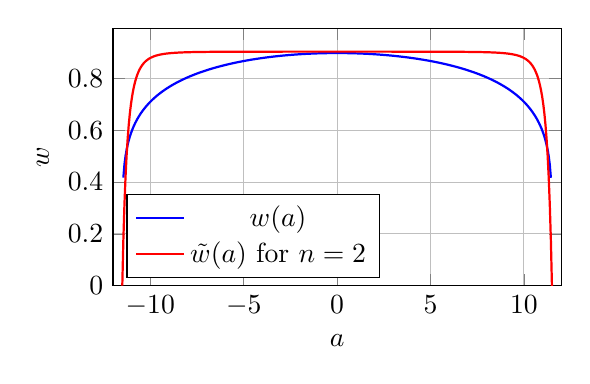
\begin{tikzpicture}
		\begin{axis}[
				xlabel={$a$},
				ylabel={$w$},
				width=0.6\textwidth,
				height=0.4\textwidth,
				grid=major,
				legend pos=south west,
				xmin=-12, xmax=12,
				ymin=0
			]
			\addplot[domain=-11.5:11.5,samples=400, blue, thick] { (1/14)*((51.282*sqrt(132.25 - x^2))^(1/3)) + (1/0.910)*(1.667*sqrt(132.25 - x^2))*((51.282*sqrt(132.25 - x^2))^(-2/3)) };
			\addlegendentry{$w(a)$}
			\addplot[domain=-11.5:11.5,samples=400,red, thick] { 0.9040595325562741-1/((abs(x)-12.525535603937156)^4) };
			\addlegendentry{$\tilde{w}(a)$ for $n=2$}
		\end{axis}
	\end{tikzpicture}
	\caption{Plot of $w$ versus $a$ and its approximation.}
	\label{fig:w_vs_a}
\end{figure}

% \pgfkeys{/pgf/fpu=true}
The following Figure \ref{fig:resulting_diamonds} visualizes the friction circle \eqref{eq:friction_circle}, its tighter constraint
\eqref{eq:friction_circle_stricter} and the resulting diamond-shaped bounds for $v$ and $\delta$ for a fixed value of $a$.

\begin{figure}[h!]
	\centering
	\begin{subfigure}{0.49\textwidth}
		\centering
		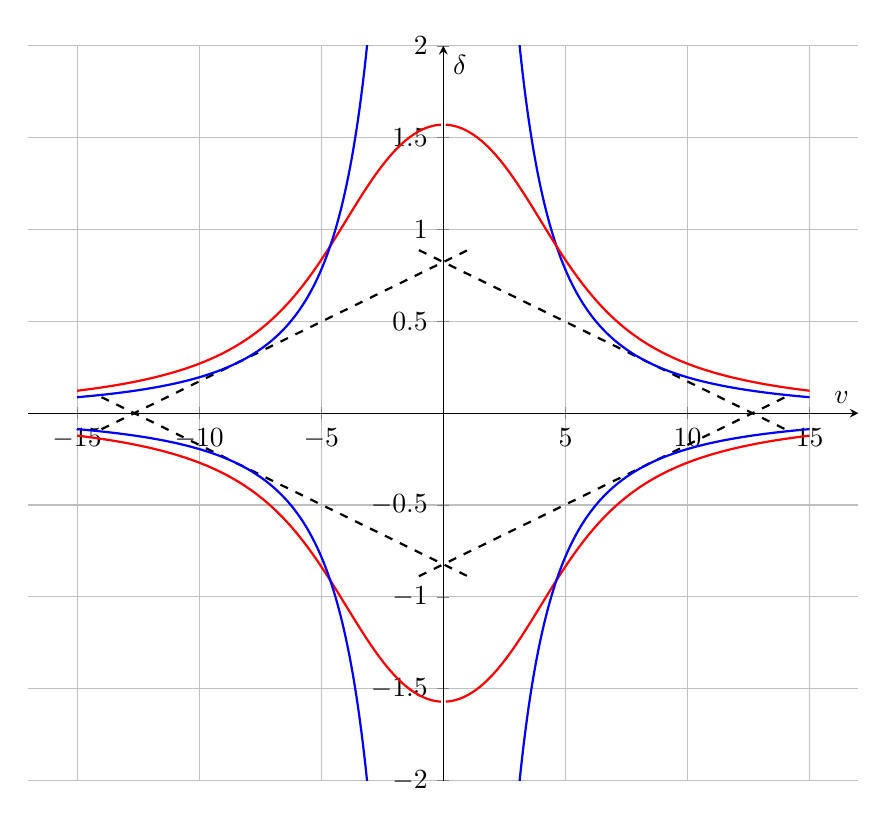
\begin{tikzpicture}
			\begin{axis}[
					xlabel={$v$},
					ylabel={$\delta$},
					width=\textwidth,
					height=0.9\textwidth,
					axis lines=middle,
					grid=major,
					legend pos=north west,
					xmin=-17, xmax=17,
					ymin=-2, ymax=2,
					legend to name=namedlegend, % Shared legend
					legend style={draw=none, cells={anchor=west}, font=\footnotesize},
				]

				% Define constants
				\def\vmax{14}
				\def\deltaMax{0.91}
				\def\lwb{2.4}
				\def\amax{11.5}
				\def\avar{0}

				% Diamond constraints
				\def\dv{1/\vmax}
				\def\ddelta{1/\deltaMax}
				\def\wvar{0.9040595325562741}

				\addplot[domain=-1:14, samples=400, dashed, thick, black]
				({x},{(\wvar-\dv*x )*\deltaMax});

				% Improved friction constraint
				\addplot[domain=2:15, samples=200, thick, blue]
				({x}, {sqrt(\amax^2 - \avar^2) * (1/(x^2)) * (\lwb * \deltaMax) / tan(\deltaMax r)});

				% Friction-circle constraints
				\addplot[domain=0.1:15, samples=200, thick, red]
				({x}, {rad(atan(\amax*\lwb/(x^2)))});

				\addplot[domain=-1:14, samples=400, dashed, thick, black]
				({x},{(\dv*x-\wvar )*\deltaMax});

				\addplot[domain=-14:1, samples=400, dashed, thick, black]
				({x},{(\wvar+\dv*x )*\deltaMax});

				\addplot[domain=-14:1, samples=400, dashed, thick, black]
				({x},{(-\wvar - \dv*x )*\deltaMax});

				% Friction-circle constraints
				\addplot[domain=0.1:15, samples=200, thick, red]
				({x}, {-rad(atan(\amax*\lwb/(x^2)))});

				\addplot[domain=-15:-0.1, samples=200, thick, red]
				({x}, {rad(atan(\amax*\lwb/(x^2)))});

				\addplot[domain=-15:-0.1, samples=200, thick, red]
				({x}, {-rad(atan(\amax*\lwb/(x^2)))});

				% Improved friction constraint
				\addplot[domain=-15:-2, samples=200, thick, blue]
				({x}, {sqrt(\amax^2 - \avar^2) * (1/(x^2)) * (\lwb * \deltaMax) / tan(\deltaMax r)});

				\addplot[domain=2:15, samples=200, thick, blue]
				({x}, {-sqrt(\amax^2 - \avar^2) * (1/(x^2)) * (\lwb * \deltaMax) / tan(\deltaMax r)});

				\addplot[domain=-15:-2, samples=200, thick, blue]
				({x}, {-sqrt(\amax^2 - \avar^2) * (1/(x^2)) * (\lwb * \deltaMax) / tan(\deltaMax r)});

				% Define legend
				\legend{Diamond Constraint, Tighter Friction Constraint, Friction Constraint}
			\end{axis}
		\end{tikzpicture}
		\caption{Plot of the resulting diamond at $a=0$.}
		\label{fig:resulting_diamond_0}
	\end{subfigure}
	\hfill
	\begin{subfigure}{0.49\textwidth}
		\centering
		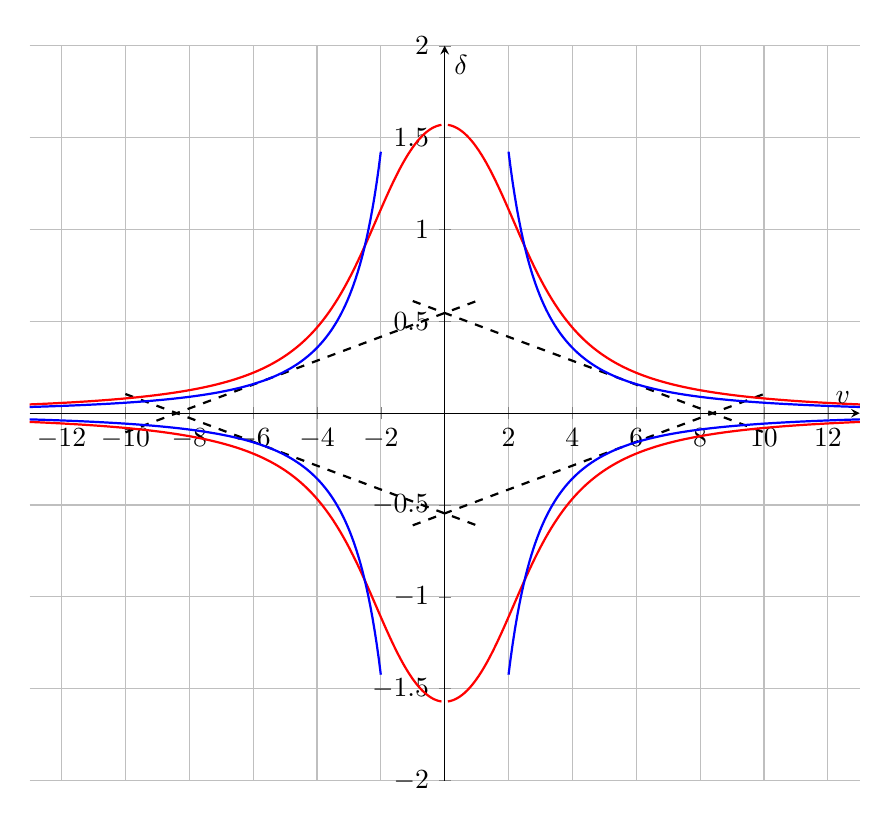
\begin{tikzpicture}
			\begin{axis}[
					xlabel={$v$},
					ylabel={$\delta$},
					width=\textwidth,
					height=0.9\textwidth,
					axis lines=middle,
					grid=major,
					legend pos=north west,
					xmin=-13, xmax=13,
					ymin=-2, ymax=2,
				]

				% Define constants
				\def\vmax{14}
				\def\deltaMax{0.91}
				\def\lwb{2.4}
				\def\amax{11.5}
				\def\avar{11}

				% Diamond constraints
				\def\dv{1/\vmax}
				\def\ddelta{1/\deltaMax}
				\def\wvar{0.5995469115149037}

				\addplot[domain=-1:10, samples=400, dashed, thick, black]
				({x},{(\wvar-\dv*x )*\deltaMax});

				\addplot[domain=-1:10, samples=400, dashed, thick, black]
				({x},{(\dv*x-\wvar )*\deltaMax});

				\addplot[domain=-10:1, samples=400, dashed, thick, black]
				({x},{(\wvar+\dv*x )*\deltaMax});

				\addplot[domain=-10:1, samples=400, dashed, thick, black]
				({x},{(-\wvar - \dv*x )*\deltaMax});

				% Friction-circle constraints
				\addplot[domain=0.1:15, samples=200, thick, red]
				({x}, {rad(atan(sqrt(\amax^2 - \avar^2)*\lwb/(x^2)))});

				\addplot[domain=0.1:15, samples=200, thick, red]
				({x}, {-rad(atan(sqrt(\amax^2 - \avar^2)*\lwb/(x^2)))});

				\addplot[domain=-15:-0.1, samples=200, thick, red]
				({x}, {rad(atan(sqrt(\amax^2 - \avar^2)*\lwb/(x^2)))});

				\addplot[domain=-15:-0.1, samples=200, thick, red]
				({x}, {-rad(atan(sqrt(\amax^2 - \avar^2)*\lwb/(x^2)))});

				% Improved friction constraint
				\addplot[domain=2:15, samples=200, thick, blue]
				({x}, {sqrt(\amax^2 - \avar^2) * (1/(x^2)) * (\lwb * \deltaMax) / tan(\deltaMax r)});

				\addplot[domain=-15:-2, samples=200, thick, blue]
				({x}, {sqrt(\amax^2 - \avar^2) * (1/(x^2)) * (\lwb * \deltaMax) / tan(\deltaMax r)});

				\addplot[domain=2:15, samples=200, thick, blue]
				({x}, {-sqrt(\amax^2 - \avar^2) * (1/(x^2)) * (\lwb * \deltaMax) / tan(\deltaMax r)});

				\addplot[domain=-15:-2, samples=200, thick, blue]
				({x}, {-sqrt(\amax^2 - \avar^2) * (1/(x^2)) * (\lwb * \deltaMax) / tan(\deltaMax r)});
			\end{axis}
		\end{tikzpicture}
		\caption{Plot of the resulting diamond at $a=11$.}
		\label{fig:resulting_diamond_1}
	\end{subfigure}
	% Shared legend
	\ref{namedlegend}
	\caption{Comparison of the resulting diamond constraints for different acceleration values.}
	\label{fig:resulting_diamonds}
\end{figure}

In conclusion, this approach constructs a convex approximation of the friction circle and allows for weighting either $v$ or $\delta$ by setting
$v^*$.
The final constraint can be stated as follows:
\begin{equation}
	a^2 + (\frac{1}{l_{wb}}\frac{\tan(\delta^*)}{\delta^*})^2 w \leq a_{max}^2
	\label{eq:final_friction_circle}
\end{equation}
where $w$ is new introduced auxiliary variable, which is bounded by:
\begin{equation}
	0 \leq w \leq \tilde{w}(a)
	\label{eq:final_friction_circle_bounds}
\end{equation}
Our final model is now complete and ready for use in the optimization process.
It is represented by the tuple
\begin{equation}
	M_{kst}=(x_{kst}, u_{kst}, \tilde{f}_{kst}, \{w_{v,\xi}, w_{v,\delta}, w_{s,\dot{s}}, w\}, C) \label{model:kst} \end{equation} where $C$ consists of
the coupling constraints \eqref{eq:coupling_kst_0}, \eqref{eq:coupling_kst_1}, the McCormick bounds \eqref{fig:mccormick_constraints}, the introduced
hyperplanes \eqref{eq:first_hyperplane}-\eqref{eq:last_hyperplane}, and our approximated friction circle \eqref{eq:final_friction_circle} with
\eqref{eq:final_friction_circle_bounds}.

